\documentclass[8pt,handout]{beamer} 

%% Math packages
%%
\usepackage{amsmath,amsthm,amssymb}
% Removes the "Too many math alphabets used in version normal" error.
\newcommand\hmmax{0}
\newcommand\bmmax{0}
\usepackage[new]{old-arrows}
\usepackage{cancel}
\usepackage{mathdots}
\usepackage{venndiagram}
\usepackage{mathrsfs}          % Math script font

% Graphics
%%
\graphicspath{{./}{figs/}}
\usepackage{graphicx}
\usepackage{tikz}
\usetikzlibrary{arrows}
\usetikzlibrary{decorations.markings}
\usetikzlibrary{decorations.pathreplacing}
\usetikzlibrary{patterns}
\usetikzlibrary{shapes.geometric}
\usetikzlibrary{positioning}
\usetikzlibrary{matrix}
\usepackage{tikz-3dplot}
\usepackage{tkz-graph}
\usepackage{tikz-cd}

%% Colors 
%%
\usepackage{xcolor}
\usepackage{color}
\usepackage{visualalgebra}  %% Put this *after* the TikZ packages
\usepackage{visualalgebraslides}  %% Put this *after* "visualalgebra"

%% Page layout packages
%%
\usepackage{url}
\usepackage{multicol}
\usepackage{multirow}
\usepackage[numbers,square,sort&compress]{natbib}

%% Font and formatting packages
%%
\usepackage[english]{babel}    % Removing this causes compiler error
\usepackage{alltt}             % Like verbatim, but excludes \ and { }
\usepackage{enumerate}         % [shortlabels] option??
\usepackage{comment}
\usepackage{soul}              % strikeout text
\usepackage{bm}                % Bold math
\usepackage[T1]{fontenc}
\usepackage{relsize}

%% Fixes the \mathbf{} not working for fonts under 10pt
\usepackage{cmbright}
\fontencoding{OT1}\fontfamily{cmbr}\selectfont %to load ot1cmbr.fd
\DeclareFontShape{OT1}{cmbr}{bx}{n}{% change bx definition
<->cmbrbx10%
}{}
\normalfont

\makeatletter
\renewcommand*\env@matrix[1][\arraystretch]{%
  \edef\arraystretch{#1}%
  \hskip -\arraycolsep
  \let\@ifnextchar\new@ifnextchar
  \array{*\c@MaxMatrixCols c}}
\makeatother


%%=======================================================================

%% Beamer packages
%%
\mode<presentation>
{
  \usetheme{boadilla} 
  \useinnertheme{rectangles}
  \usecolortheme{dolphin}
}

\setbeamersize{text margin left=6mm}
\setbeamersize{text margin right=6mm}
\setbeamersize{sidebar width right=0mm}
\setbeamersize{sidebar width left=0mm}
\setbeamertemplate{navigation symbols}{}

\def\newblock{\hskip .11em plus .33em minus .07em}

% Other options: ball, circle, square 
\setbeamertemplate{enumerate items}[default]
%\setbeamercolor{enumerate subitem}{fg=red!80!black}
\def\opacity{0.5}
%\setbeamercovered{transparent}
\setbeamercovered{invisible}

\newcommand{\Pause}{}      %% Comment this out => lots more page breaks


\AtBeginSection[]{
  \begin{frame}
  \vfill
  \centering
  \begin{beamercolorbox}[sep=8pt,center,shadow=true,rounded=true]{title}
    \usebeamerfont{title}\insertsectionhead\par%
  \end{beamercolorbox}
  \vfill
  \end{frame}
}

%%====================================================================

\title[Group actions!]{Group actions!}

\author[\href{mailto:sbagley@westminsteru.edu}{S. Bagley}]
       {\href{mailto:sbagley@westminsteru.edu}{Spencer Bagley}}

\institute[Westminster] { 
  \normalsize With many thanks to Matthew Macauley, \\
  \url{http://www.math.clemson.edu/~macaule/}}

\date[7 Apr 2025]{7 Apr 2025}

\begin{document}

\frame{\titlepage}


%%====================================================================

%\end{document}

%%====================================================================

\begin{frame}{Overview} %\Pause

  Intuitively, a \Alert{group action} occurs when a group $G$
  ``naturally permutes'' a set $S$ \emph{of states}.

  \medskip\Pause
  
  For example: \smallskip
  \begin{itemize}
  \item The ``Rubik's cube group'' consists of the $4.3\times 10^{19}$
    \Alert{actions} that \emph{permute} the
    $4.3\times 10^{19}$ \Balert{configurations} of the cube. \Pause
  \item The group $D_4$ consists of the 8 \Alert{symmetries} of the
    square. These symmetries are \emph{actions} that
    \emph{permute} the $8$ \Balert{configurations} of the
    square.
  \end{itemize}
  
  \medskip\Pause 
  
  Group actions formalize the interplay between the actual
  \Alert{group of actions} and the \Balert{sets of objects} that they
  ``rearrange.''
  
  \medskip\Pause
  
  There are many other examples of groups that ``act on'' sets of
  objects. We will see examples when the group and the set have
  different sizes.
  
  \medskip\pause

  The rich theory of group actions can be used to prove many deep
  results in group theory.

  \medskip\Pause

  We have actually already seen many group actions, without knowing
  it, such as: \smallskip
  \begin{itemize}
  \item groups acting on themselves by multiplication
  \item groups acting on themselves by conjugation
  \item groups acting on their subgroups by conjugation
  \item groups acting on cosets by multiplication
  \item automorphism groups acting on groups.
  \end{itemize}
  
\end{frame}

%%====================================================================

\begin{frame}{Actions vs.\ configurations}

  The group $D_4$ can be thought of as the 8 \Alert{symmetries} of the
  square:\quad     
  \begin{tikzpicture}[scale=.75,baseline=2ex]
    \path[fill=actRed] (0,.5) rectangle ++(.5,.5); 
    \path[fill=actYellow] (.5,.5) rectangle ++(.5,.5);
    \path[fill=actGreen] (0,0) rectangle ++(.5,.5);
    \path[fill=actBlue] (.5,0) rectangle ++(.5,.5);
    \draw (0,0) rectangle (1,1);
    \draw (.25,.75) node{$1$}; \draw (.75,.75) node{$2$};
    \draw (.25,.25) node{$4$}; \draw (.75,.25) node{$3$};
  \end{tikzpicture}

  \bigskip\Pause

  There is a subtle but \emph{important} distinction to make, between
  the actual 8 \Alert{symmetries} of the square, and the 8
  \Balert{configurations}. 
  
  \medskip\Pause

  For example, the 8 \Alert{symmetries} (alternatively, ``actions'')
  can be thought of as
  \[
  1,\qquad r,\qquad r^2,\qquad r^3,\qquad f,\qquad rf,\qquad r^2f,\qquad r^3f\,.
  \]
  \Pause The 8 \Balert{configurations} (or \emph{states}) of the
  square are the following:
  %%
  %% The 8 configurations of colored square w/ 1,2,3,4 labels
  \[
    \begin{tikzpicture}[scale=.75]
      \path[fill=actRed] (0,.5) rectangle ++(.5,.5); 
      \path[fill=actYellow] (.5,.5) rectangle ++(.5,.5);
      \path[fill=actGreen] (0,0) rectangle ++(.5,.5);
      \path[fill=actBlue] (.5,0) rectangle ++(.5,.5);
      \draw (.25,.75) node{$1$}; \draw (.75,.75) node{$2$};
      \draw (.25,.25) node{$4$}; \draw (.75,.25) node{$3$};
      \draw (0,0) rectangle (1,1);
    \end{tikzpicture}
    \qquad
    \begin{tikzpicture}[scale=.75]
      \path[fill=actGreen] (0,.5) rectangle ++(.5,.5); 
      \path[fill=actRed] (.5,.5) rectangle ++(.5,.5);
      \path[fill=actBlue] (0,0) rectangle ++(.5,.5);
      \path[fill=actYellow] (.5,0) rectangle ++(.5,.5);
      \draw (0,0) rectangle (1,1);
      \draw (.25,.75) node{$4$}; \draw (.75,.75) node{$1$};
        \draw (.25,.25) node{$3$}; \draw (.75,.25) node{$2$};
    \end{tikzpicture}
    \qquad
    \begin{tikzpicture}[scale=.75]
      \path[fill=actBlue] (0,.5) rectangle ++(.5,.5); 
      \path[fill=actGreen] (.5,.5) rectangle ++(.5,.5);
      \path[fill=actYellow] (0,0) rectangle ++(.5,.5);
      \path[fill=actRed] (.5,0) rectangle ++(.5,.5);
      \draw (0,0) rectangle (1,1);
      \draw (.25,.75) node{$3$}; \draw (.75,.75) node{$4$};
        \draw (.25,.25) node{$2$}; \draw (.75,.25) node{$1$};
    \end{tikzpicture}
    \qquad
    \begin{tikzpicture}[scale=.75]
      \path[fill=actYellow] (0,.5) rectangle ++(.5,.5); 
      \path[fill=actBlue] (.5,.5) rectangle ++(.5,.5);
      \path[fill=actRed] (0,0) rectangle ++(.5,.5);
      \path[fill=actGreen] (.5,0) rectangle ++(.5,.5);
      \draw (0,0) rectangle (1,1);
      \draw (.25,.75) node{$2$}; \draw (.75,.75) node{$3$};
      \draw (.25,.25) node{$1$}; \draw (.75,.25) node{$4$};
    \end{tikzpicture}
    \qquad
    \begin{tikzpicture}[scale=.75]
      \path[fill=actYellow] (0,.5) rectangle ++(.5,.5); 
      \path[fill=actRed] (.5,.5) rectangle ++(.5,.5);
      \path[fill=actBlue] (0,0) rectangle ++(.5,.5);
      \path[fill=actGreen] (.5,0) rectangle ++(.5,.5);
      \draw (0,0) rectangle (1,1);
      \draw (.25,.75) node{$2$}; \draw (.75,.75) node{$1$};
      \draw (.25,.25) node{$3$}; \draw (.75,.25) node{$4$};
    \end{tikzpicture}
    \qquad
    \begin{tikzpicture}[scale=.75]
      \path[fill=actBlue] (0,.5) rectangle ++(.5,.5); 
      \path[fill=actYellow] (.5,.5) rectangle ++(.5,.5);
      \path[fill=actGreen] (0,0) rectangle ++(.5,.5);
      \path[fill=actRed] (.5,0) rectangle ++(.5,.5);
      \draw (0,0) rectangle (1,1);
      \draw (.25,.75) node{$3$}; \draw (.75,.75) node{$2$};
        \draw (.25,.25) node{$4$}; \draw (.75,.25) node{$1$};
    \end{tikzpicture}
    \qquad
    \begin{tikzpicture}[scale=.75]
      \path[fill=actGreen] (0,.5) rectangle ++(.5,.5); 
      \path[fill=actBlue] (.5,.5) rectangle ++(.5,.5);
      \path[fill=actRed] (0,0) rectangle ++(.5,.5);
      \path[fill=actYellow] (.5,0) rectangle ++(.5,.5);
      \draw (0,0) rectangle (1,1);
      \draw (.25,.75) node{$4$}; \draw (.75,.75) node{$3$};
      \draw (.25,.25) node{$1$}; \draw (.75,.25) node{$2$};
    \end{tikzpicture}
    \qquad
    \begin{tikzpicture}[scale=.75]
      \path[fill=actRed] (0,.5) rectangle ++(.5,.5); 
      \path[fill=actGreen] (.5,.5) rectangle ++(.5,.5);
      \path[fill=actYellow] (0,0) rectangle ++(.5,.5);
      \path[fill=actBlue] (.5,0) rectangle ++(.5,.5);
      \draw (0,0) rectangle (1,1);
      \draw (.25,.75) node{$1$}; \draw (.75,.75) node{$4$};
      \draw (.25,.25) node{$2$}; \draw (.75,.25) node{$3$};
    \end{tikzpicture}
    \]

  \medskip\Pause

  When we were just learning about groups, we made an \Alert{action
    graph}. \smallskip

  %\Pause

  \begin{itemize}
    \item The \Balert{vertices} corresponded to the
      \Balert{states}. \smallskip\Pause
    \item The \Alert{edges} corresponded to \Alert{generators}. \smallskip\Pause
    \item The \Palert{paths} corresponded to \Palert{actions} (group
      elements).
  \end{itemize}

\end{frame}


%%====================================================================

\section{Action graphs!}

%%====================================================================

\begin{frame}{Action graph of $D_4$}
  
  Here is the \Alert{action graph} of the group
  $D_4=\<\Alert{r},\Balert{f}\>$:

  %% Cayley graph (action graph) of D_4 with configurations of the square
    \[  
    \begin{tikzpicture}
      \begin{scope}[shift={(-5,-1.25)},scale=.8]
        \tikzstyle{v} = [circle, draw, fill=lightgray,inner sep=0pt, 
          minimum size=5.75mm]
        \node at (.5,3) {\emph{``Group switchboard''}};
        \draw [midgray,fill=vYellow!50,rounded corners] (-.5,-1.5)
        rectangle ++(2,4); 
        \node at (0,2) [v] {$1$}; \node at (1,2) [v,fill=vBlue] {$f$};
        \node at (0,1) [v,fill=vRed] {$r$}; \node at (1,1) [v] {$rf$};
        \node at (0,0) [v] {$r^2$}; \node at (1,0) [v] {$r^2\!f$};
        \node at (0,-1) [v] {$r^3$}; \node at (1,-1) [v] {$r^3\!f$};
      \end{scope}
      %%
      \begin{scope}[scale=.65]
      \path[fill=actRed] (0,.5) rectangle ++(.5,.5); 
      \path[fill=actYellow] (.5,.5) rectangle ++(.5,.5);
      \path[fill=actGreen] (0,0) rectangle ++(.5,.5);
      \path[fill=actBlue] (.5,0) rectangle ++(.5,.5);
      \draw (.25,.75) node{$1$}; \draw (.75,.75) node{$2$};
      \draw (.25,.25) node{$4$}; \draw (.75,.25) node{$3$};
      \draw (0,0) rectangle (1,1);
      \begin{scope}[shift={(3,0)}]
        \path[fill=actGreen] (0,.5) rectangle ++(.5,.5); 
        \path[fill=actRed] (.5,.5) rectangle ++(.5,.5);
        \path[fill=actBlue] (0,0) rectangle ++(.5,.5);
        \path[fill=actYellow] (.5,0) rectangle ++(.5,.5);
        \draw (0,0) rectangle (1,1);
        \draw (.25,.75) node{$4$}; \draw (.75,.75) node{$1$};
        \draw (.25,.25) node{$3$}; \draw (.75,.25) node{$2$};
      \end{scope}
      \begin{scope}[shift={(3,-3)}]
        \path[fill=actBlue] (0,.5) rectangle ++(.5,.5); 
        \path[fill=actGreen] (.5,.5) rectangle ++(.5,.5);
        \path[fill=actYellow] (0,0) rectangle ++(.5,.5);
        \path[fill=actRed] (.5,0) rectangle ++(.5,.5);
        \draw (0,0) rectangle (1,1);
        \draw (.25,.75) node{$3$}; \draw (.75,.75) node{$4$};
        \draw (.25,.25) node{$2$}; \draw (.75,.25) node{$1$};
      \end{scope}
      \begin{scope}[shift={(0,-3)}]
        \path[fill=actYellow] (0,.5) rectangle ++(.5,.5); 
        \path[fill=actBlue] (.5,.5) rectangle ++(.5,.5);
        \path[fill=actRed] (0,0) rectangle ++(.5,.5);
        \path[fill=actGreen] (.5,0) rectangle ++(.5,.5);
        \draw (0,0) rectangle (1,1);
        \draw (.25,.75) node{$2$}; \draw (.75,.75) node{$3$};
        \draw (.25,.25) node{$1$}; \draw (.75,.25) node{$4$};
      \end{scope}
      \begin{scope}[shift={(-2,2)}]
        \path[fill=actYellow] (0,.5) rectangle ++(.5,.5); 
        \path[fill=actRed] (.5,.5) rectangle ++(.5,.5);
        \path[fill=actBlue] (0,0) rectangle ++(.5,.5);
        \path[fill=actGreen] (.5,0) rectangle ++(.5,.5);
        \draw (0,0) rectangle (1,1);
        \draw (.25,.75) node{$2$}; \draw (.75,.75) node{$1$};
        \draw (.25,.25) node{$3$}; \draw (.75,.25) node{$4$};
      \end{scope}
      \begin{scope}[shift={(-2,-5)}]
        \path[fill=actBlue] (0,.5) rectangle ++(.5,.5); 
        \path[fill=actYellow] (.5,.5) rectangle ++(.5,.5);
        \path[fill=actGreen] (0,0) rectangle ++(.5,.5);
        \path[fill=actRed] (.5,0) rectangle ++(.5,.5);
        \draw (0,0) rectangle (1,1);
        \draw (.25,.75) node{$3$}; \draw (.75,.75) node{$2$};
        \draw (.25,.25) node{$4$}; \draw (.75,.25) node{$1$};
      \end{scope}
      \begin{scope}[shift={(5,-5)}]
        \path[fill=actGreen] (0,.5) rectangle ++(.5,.5); 
        \path[fill=actBlue] (.5,.5) rectangle ++(.5,.5);
        \path[fill=actRed] (0,0) rectangle ++(.5,.5);
        \path[fill=actYellow] (.5,0) rectangle ++(.5,.5);
        \draw (0,0) rectangle (1,1);
        \draw (.25,.75) node{$4$}; \draw (.75,.75) node{$3$};
        \draw (.25,.25) node{$1$}; \draw (.75,.25) node{$2$};
      \end{scope}
      \begin{scope}[shift={(5,2)}]
        \path[fill=actRed] (0,.5) rectangle ++(.5,.5); 
        \path[fill=actGreen] (.5,.5) rectangle ++(.5,.5);
        \path[fill=actYellow] (0,0) rectangle ++(.5,.5);
        \path[fill=actBlue] (.5,0) rectangle ++(.5,.5);
        \draw (0,0) rectangle (1,1);
        \draw (.25,.75) node{$1$}; \draw (.75,.75) node{$4$};
        \draw (.25,.25) node{$2$}; \draw (.75,.25) node{$3$};
      \end{scope}
      \draw [r] (1,.5) to (3,.5);
      \draw [r] (3.5,0) to (3.5,-2);
      \draw [r] (3,-2.5) to (1,-2.5);
      \draw [r] (.5,-2) to (.5,0);
      \draw [r] (-1.5,2) to (-1.5,-4);
      \draw [r] (-1,-4.5) to (5,-4.5);
      \draw [r] (5.5,-4) to (5.5,2);
      \draw [r] (5,2.5) to (-1,2.5);
      \draw [bb] (0,1) to (-1,2);
      \draw [bb] (4,1) to (5,2);
      \draw [bb] (4,-3) to (5,-4);
      \draw [bb] (0,-3) to (-1,-4);
      \end{scope}
    \end{tikzpicture}
    \]
  
  %\vspace{-1mm}\Pause
  
  In the beginning of this course, we picked a configuration to be the
  ``solved state,'' and this gave us a \emph{bijection} between \Balert{
    configurations} and \Alert{actions} (group elements). 

  \medskip\Pause 

  The resulting graph was a Cayley graph.
  

\end{frame}


%%====================================================================
\begin{frame}{Action graphs}

  In all of the examples we saw in the beginning of the course, we had
  a bijective correspondence between actions and configurations. \emph{This
    need not always happen!}

  \medskip\Pause

  Suppose we have a size-$7$ set consisting of the following ``binary
  squares.''

  %% Set of 7 binary squares
  \[
  \begin{tikzpicture}[scale=.65]
    \node at (-1,.5) {$S=\Bigg\{$};
    \node at (13.5,.5) {$\Bigg\}$};
    \node at (1.5,.25) {,};
    \node at (3.5,.25) {,};
    \node at (5.5,.25) {,};
    \node at (7.5,.25) {,};
    \node at (9.5,.25) {,};
    \node at (11.5,.25) {,};
    %%
    \begin{scope}[shift={(0,0)}]
      \path[fill=actOrange] (0,.5) rectangle ++(.5,.5); 
      \path[fill=actOrange] (.5,.5) rectangle ++(.5,.5);
      \path[fill=actOrange] (0,0) rectangle ++(.5,.5);
      \path[fill=actOrange] (.5,0) rectangle ++(.5,.5);
      \draw (.25,.75) node{$0$}; \draw (.75,.75) node{$0$};
      \draw (.25,.25) node{$0$}; \draw (.75,.25) node{$0$};
      \draw (0,0) rectangle (1,1);
    \end{scope}
    %%
    \begin{scope}[shift={(2,0)}]
      \path[fill=actOrange] (0,.5) rectangle ++(.5,.5); 
      \path[fill=actPurple] (.5,.5) rectangle ++(.5,.5);
      \path[fill=actPurple] (0,0) rectangle ++(.5,.5);
      \path[fill=actOrange] (.5,0) rectangle ++(.5,.5);
      \draw (0,0) rectangle (1,1);
      \draw (.25,.75) node{$0$}; \draw (.75,.75) node{$1$};
      \draw (.25,.25) node{$1$}; \draw (.75,.25) node{$0$};
    \end{scope}
    \begin{scope}[shift={(4,0)}]
      \path[fill=actPurple] (0,.5) rectangle ++(.5,.5); 
      \path[fill=actOrange] (.5,.5) rectangle ++(.5,.5);
      \path[fill=actOrange] (0,0) rectangle ++(.5,.5);
      \path[fill=actPurple] (.5,0) rectangle ++(.5,.5);
      \draw (0,0) rectangle (1,1);
      \draw (.25,.75) node{$1$}; \draw (.75,.75) node{$0$};
      \draw (.25,.25) node{$0$}; \draw (.75,.25) node{$1$};
    \end{scope}
    \begin{scope}[shift={(6,0)}]
      \path[fill=actPurple] (0,.5) rectangle ++(.5,.5); 
      \path[fill=actPurple] (.5,.5) rectangle ++(.5,.5);
      \path[fill=actOrange] (0,0) rectangle ++(.5,.5);
      \path[fill=actOrange] (.5,0) rectangle ++(.5,.5);
      \draw (0,0) rectangle (1,1);
      \draw (.25,.75) node{$1$}; \draw (.75,.75) node{$1$};
      \draw (.25,.25) node{$0$}; \draw (.75,.25) node{$0$};
    \end{scope}
    \begin{scope}[shift={(8,0)}]
      \path[fill=actOrange] (0,.5) rectangle ++(.5,.5); 
      \path[fill=actPurple] (.5,.5) rectangle ++(.5,.5);
      \path[fill=actOrange] (0,0) rectangle ++(.5,.5);
      \path[fill=actPurple] (.5,0) rectangle ++(.5,.5);
      \draw (0,0) rectangle (1,1);
      \draw (.25,.75) node{$0$}; \draw (.75,.75) node{$1$};
      \draw (.25,.25) node{$0$}; \draw (.75,.25) node{$1$};
    \end{scope}
    \begin{scope}[shift={(10,0)}]
      \path[fill=actOrange] (0,.5) rectangle ++(.5,.5); 
      \path[fill=actOrange] (.5,.5) rectangle ++(.5,.5);
      \path[fill=actPurple] (0,0) rectangle ++(.5,.5);
      \path[fill=actPurple] (.5,0) rectangle ++(.5,.5);
      \draw (0,0) rectangle (1,1);
      \draw (.25,.75) node{$0$}; \draw (.75,.75) node{$0$};
        \draw (.25,.25) node{$1$}; \draw (.75,.25) node{$1$};
    \end{scope}
    \begin{scope}[shift={(12,0)}]
      \path[fill=actPurple] (0,.5) rectangle ++(.5,.5); 
      \path[fill=actOrange] (.5,.5) rectangle ++(.5,.5);
      \path[fill=actPurple] (0,0) rectangle ++(.5,.5);
      \path[fill=actOrange] (.5,0) rectangle ++(.5,.5);
      \draw (0,0) rectangle (1,1);
      \draw (.25,.75) node{$1$}; \draw (.75,.75) node{$0$};
      \draw (.25,.25) node{$1$}; \draw (.75,.25) node{$0$};
    \end{scope}
  \end{tikzpicture}
  \]

  \Pause%\vspace{-2mm}

  Let's see what happens to these binary squares when we push different buttons on the $D_4$ ``group switchboard.''

  \[
  \begin{tikzpicture}[scale=.65]
      \tikzstyle{v} = [circle, draw, fill=lightgray,inner sep=0pt, 
        minimum size=5.5mm]
      \node at (.5,4) {\small \emph{``Group switchboard''}};
      \draw [midgray,fill=vYellow!50,rounded corners] (-.5,-.5)
      rectangle ++(2,4); 
      \node at (0,3) [v] {$1$}; \node at (1,3) [v,fill=vBlue] {$f$};
      \node at (0,2) [v,fill=vRed] {$r$}; \node at (1,2) [v] {$rf$};
      \node at (0,1) [v] {$r^2$}; \node at (1,1) [v] {$r^2\!f$};
      \node at (0,0) [v] {$r^3$}; \node at (1,0) [v] {$r^3\!f$};
  \end{tikzpicture}
  \]

\end{frame}

%%====================================================================

\begin{frame}{Action graphs}

  In all of the examples we saw in the beginning of the course, we had
  a bijective correspondence between actions and states. \emph{This
    need not always happen!}

  \medskip

  Suppose we have a size-$7$ set consisting of the following ``binary
  squares.''

  %% Set of 7 binary squares
  \[
  \begin{tikzpicture}[scale=.65]
    \node at (-1,.5) {$S=\Bigg\{$};
    \node at (13.5,.5) {$\Bigg\}$};
    \node at (1.5,.25) {,};
    \node at (3.5,.25) {,};
    \node at (5.5,.25) {,};
    \node at (7.5,.25) {,};
    \node at (9.5,.25) {,};
    \node at (11.5,.25) {,};
    %%
    \begin{scope}[shift={(0,0)}]
      \path[fill=actOrange] (0,.5) rectangle ++(.5,.5); 
      \path[fill=actOrange] (.5,.5) rectangle ++(.5,.5);
      \path[fill=actOrange] (0,0) rectangle ++(.5,.5);
      \path[fill=actOrange] (.5,0) rectangle ++(.5,.5);
      \draw (.25,.75) node{$0$}; \draw (.75,.75) node{$0$};
      \draw (.25,.25) node{$0$}; \draw (.75,.25) node{$0$};
      \draw (0,0) rectangle (1,1);
    \end{scope}
    %%
    \begin{scope}[shift={(2,0)}]
      \path[fill=actOrange] (0,.5) rectangle ++(.5,.5); 
      \path[fill=actPurple] (.5,.5) rectangle ++(.5,.5);
      \path[fill=actPurple] (0,0) rectangle ++(.5,.5);
      \path[fill=actOrange] (.5,0) rectangle ++(.5,.5);
      \draw (0,0) rectangle (1,1);
      \draw (.25,.75) node{$0$}; \draw (.75,.75) node{$1$};
      \draw (.25,.25) node{$1$}; \draw (.75,.25) node{$0$};
    \end{scope}
    \begin{scope}[shift={(4,0)}]
      \path[fill=actPurple] (0,.5) rectangle ++(.5,.5); 
      \path[fill=actOrange] (.5,.5) rectangle ++(.5,.5);
      \path[fill=actOrange] (0,0) rectangle ++(.5,.5);
      \path[fill=actPurple] (.5,0) rectangle ++(.5,.5);
      \draw (0,0) rectangle (1,1);
      \draw (.25,.75) node{$1$}; \draw (.75,.75) node{$0$};
      \draw (.25,.25) node{$0$}; \draw (.75,.25) node{$1$};
    \end{scope}
    \begin{scope}[shift={(6,0)}]
      \path[fill=actPurple] (0,.5) rectangle ++(.5,.5); 
      \path[fill=actPurple] (.5,.5) rectangle ++(.5,.5);
      \path[fill=actOrange] (0,0) rectangle ++(.5,.5);
      \path[fill=actOrange] (.5,0) rectangle ++(.5,.5);
      \draw (0,0) rectangle (1,1);
      \draw (.25,.75) node{$1$}; \draw (.75,.75) node{$1$};
      \draw (.25,.25) node{$0$}; \draw (.75,.25) node{$0$};
    \end{scope}
    \begin{scope}[shift={(8,0)}]
      \path[fill=actOrange] (0,.5) rectangle ++(.5,.5); 
      \path[fill=actPurple] (.5,.5) rectangle ++(.5,.5);
      \path[fill=actOrange] (0,0) rectangle ++(.5,.5);
      \path[fill=actPurple] (.5,0) rectangle ++(.5,.5);
      \draw (0,0) rectangle (1,1);
      \draw (.25,.75) node{$0$}; \draw (.75,.75) node{$1$};
      \draw (.25,.25) node{$0$}; \draw (.75,.25) node{$1$};
    \end{scope}
    \begin{scope}[shift={(10,0)}]
      \path[fill=actOrange] (0,.5) rectangle ++(.5,.5); 
      \path[fill=actOrange] (.5,.5) rectangle ++(.5,.5);
      \path[fill=actPurple] (0,0) rectangle ++(.5,.5);
      \path[fill=actPurple] (.5,0) rectangle ++(.5,.5);
      \draw (0,0) rectangle (1,1);
      \draw (.25,.75) node{$0$}; \draw (.75,.75) node{$0$};
        \draw (.25,.25) node{$1$}; \draw (.75,.25) node{$1$};
    \end{scope}
    \begin{scope}[shift={(12,0)}]
      \path[fill=actPurple] (0,.5) rectangle ++(.5,.5); 
      \path[fill=actOrange] (.5,.5) rectangle ++(.5,.5);
      \path[fill=actPurple] (0,0) rectangle ++(.5,.5);
      \path[fill=actOrange] (.5,0) rectangle ++(.5,.5);
      \draw (0,0) rectangle (1,1);
      \draw (.25,.75) node{$1$}; \draw (.75,.75) node{$0$};
      \draw (.25,.25) node{$1$}; \draw (.75,.25) node{$0$};
    \end{scope}
  \end{tikzpicture}
  \]

  The group $D_4=\<\Alert{r},\Balert{f}\>$ ``acts on $S$'' as follows:
  %%
  %%
  %% Action graph of D_4 acting on our 7 binary squares
  \[
  \begin{tikzpicture}[scale=.65]
    %%
    %% Group switchboard
    %%
    \begin{scope}[shift={(-4,.5)},scale=1]
      \tikzstyle{v} = [circle, draw, fill=lightgray,inner sep=0pt, 
        minimum size=5.5mm]
      \node at (.5,4) {\small \emph{``Group switchboard''}};
      \draw [midgray,fill=vYellow!50,rounded corners] (-.5,-.5)
      rectangle ++(2,4); 
      \node at (0,3) [v] {$1$}; \node at (1,3) [v,fill=vBlue] {$f$};
      \node at (0,2) [v,fill=vRed] {$r$}; \node at (1,2) [v] {$rf$};
      \node at (0,1) [v] {$r^2$}; \node at (1,1) [v] {$r^2\!f$};
      \node at (0,0) [v] {$r^3$}; \node at (1,0) [v] {$r^3\!f$};
    \end{scope}
    %%
    %% Size-1 component
    %%
    \begin{scope}[shift={(0,0)}]
      \path[fill=actOrange] (0,.5) rectangle ++(.5,.5); 
      \path[fill=actOrange] (.5,.5) rectangle ++(.5,.5);
      \path[fill=actOrange] (0,0) rectangle ++(.5,.5);
      \path[fill=actOrange] (.5,0) rectangle ++(.5,.5);
      \draw (.25,.75) node{$0$}; \draw (.75,.75) node{$0$};
      \draw (.25,.25) node{$0$}; \draw (.75,.25) node{$0$};
      \draw (0,0) rectangle (1,1);
      \Loop[dist=1.5cm,dir=NO,color=eRed](0,1);
      \Loop[dist=1.5cm,dir=NO,color=eBlue](1,1);
    \end{scope}
    %%
    %% Size-2 component
    %%
    \begin{scope}[shift={(3.25,0)}]
      \begin{scope}[shift={(0,3)}]
        \path[fill=actOrange] (0,.5) rectangle ++(.5,.5); 
        \path[fill=actPurple] (.5,.5) rectangle ++(.5,.5);
        \path[fill=actPurple] (0,0) rectangle ++(.5,.5);
        \path[fill=actOrange] (.5,0) rectangle ++(.5,.5);
        \draw (0,0) rectangle (1,1);
        \draw (.25,.75) node{$0$}; \draw (.75,.75) node{$1$};
        \draw (.25,.25) node{$1$}; \draw (.75,.25) node{$0$};
        \draw [rr] (.25,0) to (.25,-2);
        \draw [bb] (.75,0) to (.75,-2);
      \end{scope}
      \begin{scope}[shift={(0,0)}]
        \path[fill=actPurple] (0,.5) rectangle ++(.5,.5); 
        \path[fill=actOrange] (.5,.5) rectangle ++(.5,.5);
        \path[fill=actOrange] (0,0) rectangle ++(.5,.5);
        \path[fill=actPurple] (.5,0) rectangle ++(.5,.5);
        \draw (0,0) rectangle (1,1);
        \draw (.25,.75) node{$1$}; \draw (.75,.75) node{$0$};
        \draw (.25,.25) node{$0$}; \draw (.75,.25) node{$1$};
      \end{scope}
    \end{scope}
    %%
    %% Size-4 component
    %%
    \begin{scope}[shift={(7,0)}]
    \begin{scope}[shift={(0,3)}]
      \path[fill=actOrange] (0,.5) rectangle ++(.5,.5); 
      \path[fill=actOrange] (.5,.5) rectangle ++(.5,.5);
      \path[fill=actPurple] (0,0) rectangle ++(.5,.5);
      \path[fill=actPurple] (.5,0) rectangle ++(.5,.5);
      \draw (0,0) rectangle (1,1);
      \draw (.25,.75) node{$0$}; \draw (.75,.75) node{$0$};
      \draw (.25,.25) node{$1$}; \draw (.75,.25) node{$1$};
      \draw [r] (3,.5) to (1,.5);
      \Loop[dist=1.5cm,dir=WE,color=eBlue](0,.5);
    \end{scope}
    %%
    \begin{scope}[shift={(0,0)}]
      \path[fill=actOrange] (0,.5) rectangle ++(.5,.5); 
      \path[fill=actPurple] (.5,.5) rectangle ++(.5,.5);
      \path[fill=actOrange] (0,0) rectangle ++(.5,.5);
      \path[fill=actPurple] (.5,0) rectangle ++(.5,.5);
      \draw (0,0) rectangle (1,1);
      \draw (.25,.75) node{$0$}; \draw (.75,.75) node{$1$};
      \draw (.25,.25) node{$0$}; \draw (.75,.25) node{$1$};
      \draw [r] (.5,3) to (.5,1);
      \draw [bb] (1,1) to (3,3);
    \end{scope}
    %%
    \begin{scope}[shift={(3,3)}]
      \path[fill=actPurple] (0,.5) rectangle ++(.5,.5); 
      \path[fill=actOrange] (.5,.5) rectangle ++(.5,.5);
      \path[fill=actPurple] (0,0) rectangle ++(.5,.5);
      \path[fill=actOrange] (.5,0) rectangle ++(.5,.5);
      \draw (0,0) rectangle (1,1);
      \draw (.25,.75) node{$1$}; \draw (.75,.75) node{$0$};
      \draw (.25,.25) node{$1$}; \draw (.75,.25) node{$0$};
      \draw [r] (.5,-2) to (.5,0);
    \end{scope}
    \begin{scope}[shift={(3,0)}]
      \path[fill=actPurple] (0,.5) rectangle ++(.5,.5); 
      \path[fill=actPurple] (.5,.5) rectangle ++(.5,.5);
      \path[fill=actOrange] (0,0) rectangle ++(.5,.5);
      \path[fill=actOrange] (.5,0) rectangle ++(.5,.5);
      \draw (0,0) rectangle (1,1);
      \draw (.25,.75) node{$1$}; \draw (.75,.75) node{$1$};
      \draw (.25,.25) node{$0$}; \draw (.75,.25) node{$0$};
      \draw [r] (-2,.5) to (0,.5);
      \Loop[dist=1.5cm,dir=EA,color=eBlue](1,.5);
    \end{scope}
    \end{scope}
  \end{tikzpicture}
  \]

  \vspace{-2mm}\Pause

  The \Alert{action graph} above has some properties of Cayley
  graphs, but there are some fundamental differences as well.

\end{frame}

%%====================================================================

\begin{frame}{The ``group switchboard'' analogy} %\Pause

  Suppose we have a ``switchboard'' for $G$, with every element $g\in
  G$ having a ``button.''

  \bigskip\Pause 

  If $a\in G$, then pressing the $a$-button rearranges the
  objects in $S$---it is a \Alert{permutation}
  of $S$; call it $\phi(a)$.

  \bigskip\Pause 

  If $b\in G$, then pressing the $b$-button also rearranges the objects in
  $S$. Call this permutation $\phi(b)$.

  \bigskip\Pause 

  The element $ab\in G$ also has a button. We require that
  \Balert{pressing the $ab$-button does the same as
    pressing the $a$-button, followed by the $b$-button}. \Pause That
  is,
  \[
  \phi(ab)=\phi(a)\phi(b)\,,\qquad\text{for all } a,b\in G\,.
  \]
  \Pause Let $\Perm(S)$ be the group of permutations of $S$. Thus, if
  $|S|=n$, then $\Perm(S)\cong S_n$. (We typically think of
  $S_n$ as the permutations of $\{1,2,\dots,n\}$.)
  
  \medskip\Pause 
  
  \begin{block}{Definition}
    A group $G$ \Alert{acts on} a set $S$ if there is a homomorphism
    $\phi\colon G\to\Perm(S)$.
  \end{block}

\end{frame}

%%====================================================================

\begin{frame}{Action graphs and $G$-sets}
  %\Pause
  
  \begin{block}{Definition}
    A set $S$ with an action by $G$ is called a (right)
    \Alert{$G$-set}.
  \end{block}
  
  \begin{alertblock}{Big ideas}
   \begin{itemize}
    \item An action $\phi\colon G\to\Perm(S)$ endows $S$ with an
      \textbf{algebraic structure}.
    \item \emph{\Alert{Action graphs are to $G$-sets}, like how
      \Balert{Cayley graphs are to groups}.}
    \end{itemize}
  \end{alertblock}

  \vspace{-3mm}

  %% Action graph of D_4 = <r,f> acting on our 7 binary squares,
  %% labeled w/ stabilizers
  \[
  \scalebox{.85}{
  \begin{tikzpicture}[scale=.65,shorten >= -2pt, shorten <= -2pt]
    %%
    %% Group switchboard
    %%
    \begin{scope}[shift={(-9.25,-1.5)},scale=1]
      \tikzstyle{v} = [circle, draw, fill=lightgray,inner sep=0pt, 
        minimum size=5.4mm]
      \node at (.5,4) {\small \emph{``Group switchboard''}};
      \draw [midgray,fill=vYellow!50,rounded corners] (-.5,-.5)
      rectangle ++(2,4); 
      \node at (0,3) [v] {$1$}; \node at (1,3) [v,fill=vBlue] {$f$};
      \node at (0,2) [v,fill=vRed] {$r$}; \node at (1,2) [v,fill=vGreen] {$rf$};
      \node at (0,1) [v] {$r^2$}; \node at (1,1) [v] {$r^2\!f$};
      \node at (0,0) [v] {$r^3$}; \node at (1,0) [v] {$r^3\!f$};
    \end{scope}
    %%
    %% the size-1 orbit
    %%
    \begin{scope}[shift={(-5,0)},shorten >= 0pt, shorten <= 0pt]  
        \path[fill=actOrange] (-.5,0) rectangle ++(.5,.5); 
        \path[fill=actOrange] (0,0) rectangle ++(.5,.5);
        \path[fill=actOrange] (-.5,-.5) rectangle ++(.5,.5);
        \path[fill=actOrange] (0,-.5) rectangle ++(.5,.5);
        \draw (-.5,-.5) rectangle (.5,.5);
        \draw (-.25,.25) node{$0$}; \draw (.25,.25) node{$0$};
        \draw (-.25,-.25) node{$0$}; \draw (.25,-.25) node{$0$};
      \draw (-.5,-.5) rectangle (.5,.5);
      \Loop[dist=1.5cm,dir=NO,color=eRed](-.5,.5);
      \Loop[dist=1.5cm,dir=NO,color=eBlue](.5,.5);
      \node at (0,-1.2) {\normalsize $\bm{D_4\!=\!\<\Alert{r},\Balert{f}\>}$};
    \end{scope}
      %%
      %% the size-2 orbit
      %%
    \begin{scope}[shift={(0,0)},shorten >= -2pt, shorten <= -2pt] 
      \begin{scope}[shift={(1.75,0)}]  %% H
        \path[fill=actPurple] (-.5,0) rectangle ++(.5,.5); 
        \path[fill=actOrange] (0,0) rectangle ++(.5,.5);
        \path[fill=actOrange] (-.5,-.5) rectangle ++(.5,.5);
        \path[fill=actPurple] (0,-.5) rectangle ++(.5,.5);
        \draw (-.5,-.5) rectangle (.5,.5);
        \draw (-.25,.25) node{$1$}; \draw (.25,.25) node{$0$};
        \draw (-.25,-.25) node{$0$}; \draw (.25,-.25) node{$1$};
        \node (0-out) at (-.5,.1) {};
        \node (0-in) at (-.5,-.1) {};
        \node at (0,-1.2) {\normalsize $\bm{\<r^2,rf\>}$};
      \end{scope}
      %%
      \begin{scope}[shift={(-1.75,0)}] %% Hr^3
        \path[fill=actOrange] (-.5,0) rectangle ++(.5,.5); 
        \path[fill=actPurple] (0,0) rectangle ++(.5,.5);
        \path[fill=actPurple] (-.5,-.5) rectangle ++(.5,.5);
        \path[fill=actOrange] (0,-.5) rectangle ++(.5,.5);
        \draw (-.5,-.5) rectangle (.5,.5);
        \draw (-.25,.25) node{$0$}; \draw (.25,.25) node{$1$};
        \draw (-.25,-.25) node{$1$}; \draw (.25,-.25) node{$0$};
        \node (180-out) at (.5,-.1) {};
        \node (180-in) at (.5,.1) {};
        \node at (0,-1.2) {\normalsize $\bm{\<r^2,rf\>}$};
      \end{scope}
     \draw [rr] (0-out) to [bend right=15] (180-in);
     \draw [bb] (180-out) to [bend right=15] (0-in);
    \end{scope} %% end of the size-2 orbit
  %%
  %% the size-4 orbit
  %%
    \begin{scope}[shift={(7,0)},shorten >= 0pt, shorten <= 0pt]  
      \begin{scope}[shift={(1.75,0)}]  %% H
        \path[fill=actOrange] (-.5,0) rectangle ++(.5,.5); 
        \path[fill=actOrange] (0,0) rectangle ++(.5,.5);
        \path[fill=actPurple] (-.5,-.5) rectangle ++(.5,.5);
        \path[fill=actPurple] (0,-.5) rectangle ++(.5,.5);
        \draw (-.5,-.5) rectangle (.5,.5);
        \draw (-.25,.25) node{$0$}; \draw (.25,.25) node{$0$};
        \draw (-.25,-.25) node{$1$}; \draw (.25,-.25) node{$1$};
        \node (0-out) at (0,.5) {};
        \node (0-in) at (0,-.5) {};
        \Loop[dist=1.5cm,dir=EA,color=eBlue](.5,0);
        \node at (.9,.9) {\normalsize $\bm{\<f\>}$};
      \end{scope}
      %%
      \begin{scope}[shift={(0,1.75)}] %% Hr
        \path[fill=actOrange] (-.5,0) rectangle ++(.5,.5); 
        \path[fill=actPurple] (0,0) rectangle ++(.5,.5);
        \path[fill=actOrange] (-.5,-.5) rectangle ++(.5,.5);
        \path[fill=actPurple] (0,-.5) rectangle ++(.5,.5);
        \draw (-.5,-.5) rectangle (.5,.5);
        \draw (-.25,.25) node{$0$}; \draw (.25,.25) node{$1$};
        \draw (-.25,-.25) node{$0$}; \draw (.25,-.25) node{$1$};
        \node (90-out) at (-.5,0) {};
        \node (90-in) at (.5,0) {};
        \node (90-bb) at (0,-.5) {};
        \node at (-1.3,.5) {\normalsize $\bm{\<r^2f\>}$};
      \end{scope}
      %%
      \begin{scope}[shift={(-1.75,0)}] %% Hr^2
        \path[fill=actPurple] (-.5,0) rectangle ++(.5,.5); 
        \path[fill=actPurple] (0,0) rectangle ++(.5,.5);
        \path[fill=actOrange] (-.5,-.5) rectangle ++(.5,.5);
        \path[fill=actOrange] (0,-.5) rectangle ++(.5,.5);
        \draw (-.5,-.5) rectangle (.5,.5);
        \draw (-.25,.25) node{$1$}; \draw (.25,.25) node{$1$};
        \draw (-.25,-.25) node{$0$}; \draw (.25,-.25) node{$0$};
        \Loop[dist=1.5cm,dir=WE,color=eBlue](-.5,0);
        \node (180-out) at (0,-.5) {};
        \node (180-in) at (0,.5) {};
        \node at (-1.1,-1) {\normalsize $\bm{\<f\>}$};
      \end{scope}
      %%
      \begin{scope}[shift={(0,-1.75)}] %% Hr^3
        \path[fill=actPurple] (-.5,0) rectangle ++(.5,.5); 
        \path[fill=actOrange] (0,0) rectangle ++(.5,.5);
        \path[fill=actPurple] (-.5,-.5) rectangle ++(.5,.5);
        \path[fill=actOrange] (0,-.5) rectangle ++(.5,.5);
        \draw (-.5,-.5) rectangle (.5,.5);
        \draw (-.25,.25) node{$1$}; \draw (.25,.25) node{$0$};
        \draw (-.25,-.25) node{$1$}; \draw (.25,-.25) node{$0$};        
        \node (270-out) at (.5,0) {};
        \node (270-in) at (-.5,0) {};
        \node (270-bb) at (0,.5) {};
        \node at (1.2,-.5) {\normalsize $\bm{\<r^2f\>}$};
      \end{scope}
      \draw [r,shorten >= -2pt, shorten <= -2pt] (0-out)
      to [bend right=25] (90-in);
      \draw [r,shorten >= -2pt, shorten <= -2pt] (90-out)
      to [bend right=25] (180-in);
      \draw [r,shorten >= -2pt, shorten <= -2pt] (180-out)
      to [bend right=25] (270-in);
      \draw [r,shorten >= -2pt, shorten <= -2pt] (270-out)
      to [bend right=25] (0-in);
     \draw [bb] (90-bb) to (270-bb);
      \end{scope} %% end of the size-4 orbit
  \end{tikzpicture}}
  \]

  \vspace{-6mm}

  %% Action graph of D_4 = <s,t> acting on our 7 binary squares, labeled w/ stabilizers
  \[
  \hspace*{-4mm}
  \scalebox{.85}{
  \begin{tikzpicture}[scale=.65,shorten >= -2pt, shorten <= -2pt]
    %%
    %% the size-1 orbit
    %%
    \begin{scope}[shift={(-4.5,0)},shorten >= 0pt, shorten <= 0pt]  
      \path[fill=actOrange] (-.5,0) rectangle ++(.5,.5); 
      \path[fill=actOrange] (0,0) rectangle ++(.5,.5);
      \path[fill=actOrange] (-.5,-.5) rectangle ++(.5,.5);
      \path[fill=actOrange] (0,-.5) rectangle ++(.5,.5);
      \draw (-.5,-.5) rectangle (.5,.5);
      \draw (-.25,.25) node{$0$}; \draw (.25,.25) node{$0$};
      \draw (-.25,-.25) node{$0$}; \draw (.25,-.25) node{$0$};
      \draw (-.5,-.5) rectangle (.5,.5);
      \Loop[dist=1.5cm,dir=NO,color=eGreen](-.5,.5);
      \Loop[dist=1.5cm,dir=NO,color=eBlue](.5,.5);
      \node at (0,-1.2) {\normalsize $\bm{D_4\!=\!\<\Balert{s},\Galert{t}\>}$};
    \end{scope}
    %%
      %% the size-2 orbit
      %%
    \begin{scope}[shift={(0,0)}] 
      \begin{scope}[shift={(1.5,0)}]  %% H
        \path[fill=actPurple] (-.5,0) rectangle ++(.5,.5); 
        \path[fill=actOrange] (0,0) rectangle ++(.5,.5);
        \path[fill=actOrange] (-.5,-.5) rectangle ++(.5,.5);
        \path[fill=actPurple] (0,-.5) rectangle ++(.5,.5);
        \draw (-.5,-.5) rectangle (.5,.5);
        \draw (-.25,.25) node{$1$}; \draw (.25,.25) node{$0$};
        \draw (-.25,-.25) node{$0$}; \draw (.25,-.25) node{$1$};
        \node (0-out) at (-.5,.1) {};
        \node (0-in) at (-.5,-.1) {};
        \Loop[dist=1.5cm,dir=NO,color=eGreen](0,.5);
        \node at (0,-1.2) {\normalsize $\bm{\<t,sts\>}$};
      \end{scope}
      %%
      \begin{scope}[shift={(-1.5,0)}] %% Hr^3
        \path[fill=actOrange] (-.5,0) rectangle ++(.5,.5); 
        \path[fill=actPurple] (0,0) rectangle ++(.5,.5);
        \path[fill=actPurple] (-.5,-.5) rectangle ++(.5,.5);
        \path[fill=actOrange] (0,-.5) rectangle ++(.5,.5);
        \draw (-.5,-.5) rectangle (.5,.5);
        \draw (-.25,.25) node{$0$}; \draw (.25,.25) node{$1$};
        \draw (-.25,-.25) node{$1$}; \draw (.25,-.25) node{$0$};
        \node (180-out) at (.5,-.1) {};
        \node (180-in) at (.5,.1) {};
        \Loop[dist=1.5cm,dir=NO,color=eGreen](0,.5);
        \node at (0,-1.2) {\normalsize $\bm{\<t,sts\>}$};
      \end{scope}
     \draw [bb,shorten >= -2pt, shorten <= -2pt] (180-out) to (0-in);
    \end{scope} %% end of the size-2 orbit
  %%
  %% the size-4 orbit
  %%
    \begin{scope}[shift={(4.5,0)},shorten >= 0pt, shorten <= 0pt]  
      \begin{scope}[shift={(9,0)}]  %% H
        \path[fill=actOrange] (-.5,0) rectangle ++(.5,.5); 
        \path[fill=actOrange] (0,0) rectangle ++(.5,.5);
        \path[fill=actPurple] (-.5,-.5) rectangle ++(.5,.5);
        \path[fill=actPurple] (0,-.5) rectangle ++(.5,.5);
        \draw (-.5,-.5) rectangle (.5,.5);
        \draw (-.25,.25) node{$0$}; \draw (.25,.25) node{$0$};
        \draw (-.25,-.25) node{$1$}; \draw (.25,-.25) node{$1$};
        \node (4L) at (-.5,0) {};
        \Loop[dist=1.5cm,dir=NO,color=eBlue](0,.5);
        \node at (0,-1.2) {\normalsize $\bm{\<s\>}$};
      \end{scope}
      %%
      \begin{scope}[shift={(3,0)}] %% Hr
        \path[fill=actOrange] (-.5,0) rectangle ++(.5,.5); 
        \path[fill=actPurple] (0,0) rectangle ++(.5,.5);
        \path[fill=actOrange] (-.5,-.5) rectangle ++(.5,.5);
        \path[fill=actPurple] (0,-.5) rectangle ++(.5,.5);
        \draw (-.5,-.5) rectangle (.5,.5);
        \draw (-.25,.25) node{$0$}; \draw (.25,.25) node{$1$};
        \draw (-.25,-.25) node{$0$}; \draw (.25,-.25) node{$1$};
        \node (2L) at (-.5,0) {};
        \node (2R) at (.5,0) {};
        \node at (0,-1.2) {\normalsize $\bm{\<tst\>}$};
      \end{scope}
      %%
      \begin{scope}[shift={(0,0)}] %% Hr^2
        \path[fill=actPurple] (-.5,0) rectangle ++(.5,.5); 
        \path[fill=actPurple] (0,0) rectangle ++(.5,.5);
        \path[fill=actOrange] (-.5,-.5) rectangle ++(.5,.5);
        \path[fill=actOrange] (0,-.5) rectangle ++(.5,.5);
        \draw (-.5,-.5) rectangle (.5,.5);
        \draw (-.25,.25) node{$1$}; \draw (.25,.25) node{$1$};
        \draw (-.25,-.25) node{$0$}; \draw (.25,-.25) node{$0$};
        \node (1R) at (.5,0) {};
        \Loop[dist=1.5cm,dir=NO,color=eBlue](0,.5);
        \node at (0,-1.2) {\normalsize $\bm{\<s\>}$};
      \end{scope}
      %%
      \begin{scope}[shift={(6,0)}] %% Hr^3
        \path[fill=actPurple] (-.5,0) rectangle ++(.5,.5); 
        \path[fill=actOrange] (0,0) rectangle ++(.5,.5);
        \path[fill=actPurple] (-.5,-.5) rectangle ++(.5,.5);
        \path[fill=actOrange] (0,-.5) rectangle ++(.5,.5);
        \draw (-.5,-.5) rectangle (.5,.5);
        \draw (-.25,.25) node{$1$}; \draw (.25,.25) node{$0$};
        \draw (-.25,-.25) node{$1$}; \draw (.25,-.25) node{$0$};        
        \node (3L) at (-.5,0) {};
        \node (3R) at (.5,0) {};
        \node at (0,-1.2) {\normalsize $\bm{\<tst\>}$};
      \end{scope}
      \draw [gg,shorten >= -2pt, shorten <= -2pt] (1R) to (2L);
      \draw [bb,shorten >= -2pt, shorten <= -2pt] (2R) to (3L);
      \draw [gg,shorten >= -2pt, shorten <= -2pt] (3R) to (4L);
      \end{scope} %% end of the size-4 orbit
  \end{tikzpicture}}
  \]
  
\end{frame}

%%====================================================================

\begin{frame}{The ``group switchboard'' analogy} 
  
  In our binary square example, pressing the \Alert{$r$-button} and
  \Balert{$f$-button} permutes $S$ as follows:
  
  %% Permutation diagrams of \phi(r) for our binary square example
  \[
  \begin{tikzpicture}[scale=.5]
    \tikzstyle{p} = [draw,bend left=55,-stealth']
    \tikzstyle{every node}=[font=\scriptsize]
    %%
    \begin{scope}[shift={(0,0)}]
      \node at (-2.5,.5) {\normalsize {\color{xRed}$\phi(r)\;$}:};
      \path[fill=actOrange] (0,.5) rectangle ++(.5,.5); 
      \path[fill=actOrange] (.5,.5) rectangle ++(.5,.5);
      \path[fill=actOrange] (0,0) rectangle ++(.5,.5);
      \path[fill=actOrange] (.5,0) rectangle ++(.5,.5);
      \draw (.25,.75) node{$0$};\draw (.75,.75) node{$0$};
      \draw (.25,.25) node{$0$};\draw (.75,.25) node{$0$};
    \draw (0,0) rectangle (1,1);
    \end{scope}
    %%
    \begin{scope}[shift={(2.5,0)}]
      \path[fill=actOrange] (0,.5) rectangle ++(.5,.5); 
      \path[fill=actPurple] (.5,.5) rectangle ++(.5,.5);
      \path[fill=actPurple] (0,0) rectangle ++(.5,.5);
      \path[fill=actOrange] (.5,0) rectangle ++(.5,.5);
      \draw (0,0) rectangle (1,1);
      \draw(.25,.75) node{$0$};\draw(.75,.75)node{$1$};
      \draw(.25,.25) node{$1$};\draw (.75,.25)node{$0$};
      \draw [p,eRed] (.5,1) to (3,1);
    \end{scope}
    %%
    \begin{scope}[shift={(5,0)}]
      \path[fill=actPurple] (0,.5) rectangle ++(.5,.5); 
      \path[fill=actOrange] (.5,.5) rectangle ++(.5,.5);
      \path[fill=actOrange] (0,0) rectangle ++(.5,.5);
      \path[fill=actPurple] (.5,0) rectangle ++(.5,.5);
      \draw (0,0) rectangle (1,1);
      \draw(.25,.75)node{$1$};\draw (.75,.75)node{$0$};
      \draw(.25,.25)node{$0$};\draw (.75,.25)node{$1$};
      \draw [p,eRed] (.5,0) to (-2,0);
    \end{scope}
    %%
    \begin{scope}[shift={(7.5,0)}]
      \path[fill=actPurple] (0,.5) rectangle ++(.5,.5); 
      \path[fill=actPurple] (.5,.5) rectangle ++(.5,.5);
      \path[fill=actOrange] (0,0) rectangle ++(.5,.5);
      \path[fill=actOrange] (.5,0) rectangle ++(.5,.5);
      \draw (0,0) rectangle (1,1);
      \draw(.25,.75) node{$1$};\draw(.75,.75)node{$1$};
      \draw(.25,.25) node{$0$}; \draw(.75,.25)node{$0$};
      \draw [p,eRed] (.5,1) to (3,1);
    \end{scope}
    %%
    \begin{scope}[shift={(10,0)}]
      \path[fill=actPurple] (0,.5) rectangle ++(.5,.5); 
      \path[fill=actOrange] (.5,.5) rectangle ++(.5,.5);
      \path[fill=actPurple] (0,0) rectangle ++(.5,.5);
      \path[fill=actOrange] (.5,0) rectangle ++(.5,.5);
      \draw (0,0) rectangle (1,1);
      \draw(.25,.75)node{$1$};\draw(.75,.75)node{$0$};
      \draw(.25,.25)node{$1$};\draw(.75,.25) node{$0$};
      \draw [p,eRed] (.5,1) to (3,1);
    \end{scope}
    %%
    \begin{scope}[shift={(12.5,0)}]
      \path[fill=actOrange] (0,.5) rectangle ++(.5,.5); 
      \path[fill=actOrange] (.5,.5) rectangle ++(.5,.5);
      \path[fill=actPurple] (0,0) rectangle ++(.5,.5);
      \path[fill=actPurple] (.5,0) rectangle ++(.5,.5);
      \draw (0,0) rectangle (1,1);
      \draw(.25,.75)node{$0$};\draw(.75,.75) node{$0$};
      \draw(.25,.25)node{$1$};\draw(.75,.25) node{$1$};
      \draw [p,eRed] (.5,1) to (3,1);
    \end{scope}
    %%
    \begin{scope}[shift={(15,0)}]
      \path[fill=actOrange] (0,.5) rectangle ++(.5,.5); 
      \path[fill=actPurple] (.5,.5) rectangle ++(.5,.5);
      \path[fill=actOrange] (0,0) rectangle ++(.5,.5);
      \path[fill=actPurple] (.5,0) rectangle ++(.5,.5);
      \draw (0,0) rectangle (1,1);
      \draw(.25,.75)node{$0$};\draw(.75,.75) node{$1$};
      \draw(.25,.25)node{$0$};\draw(.75,.25) node{$1$};
      \draw [p,eRed,bend left=25] (.5,0) to (-7,0);
    \end{scope}
  \end{tikzpicture}
  \]

  \vspace{-6mm}\Pause

  %% Permutation diagrams of \phi(f) for our binary square example
  \[
  \begin{tikzpicture}[scale=.5]
    \tikzstyle{p} = [draw,bend left=55,-stealth]
    \tikzstyle{every node}=[font=\scriptsize]
    %%
    \begin{scope}[shift={(0,0)}]
      \node at (-2.5,.5) {\normalsize \Balert{$\phi(f)\;$}:};
      \path[fill=actOrange] (0,.5) rectangle ++(.5,.5); 
      \path[fill=actOrange] (.5,.5) rectangle ++(.5,.5);
      \path[fill=actOrange] (0,0) rectangle ++(.5,.5);
      \path[fill=actOrange] (.5,0) rectangle ++(.5,.5);
      \draw (.25,.75) node{$0$};\draw (.75,.75) node{$0$};
      \draw (.25,.25) node{$0$};\draw (.75,.25) node{$0$};
      \draw (0,0) rectangle (1,1);
    \end{scope}
    %%
    \begin{scope}[shift={(2.5,0)}]
      \path[fill=actOrange] (0,.5) rectangle ++(.5,.5); 
      \path[fill=actPurple] (.5,.5) rectangle ++(.5,.5);
      \path[fill=actPurple] (0,0) rectangle ++(.5,.5);
      \path[fill=actOrange] (.5,0) rectangle ++(.5,.5);
      \draw (0,0) rectangle (1,1);
      \draw(.25,.75) node{$0$};\draw(.75,.75)node{$1$};
      \draw(.25,.25) node{$1$};\draw (.75,.25)node{$0$};
      \draw [p,eBlue] (.5,1) to (3,1);
    \end{scope}
    %%
    \begin{scope}[shift={(5,0)}]
      \path[fill=actPurple] (0,.5) rectangle ++(.5,.5); 
      \path[fill=actOrange] (.5,.5) rectangle ++(.5,.5);
      \path[fill=actOrange] (0,0) rectangle ++(.5,.5);
      \path[fill=actPurple] (.5,0) rectangle ++(.5,.5);
      \draw (0,0) rectangle (1,1);
      \draw(.25,.75)node{$1$};\draw (.75,.75)node{$0$};
      \draw(.25,.25)node{$0$};\draw (.75,.25)node{$1$};
      \draw [p,eBlue] (.5,0) to (-2,0);
    \end{scope}
    %%
    \begin{scope}[shift={(7.5,0)}]
      \path[fill=actPurple] (0,.5) rectangle ++(.5,.5); 
      \path[fill=actPurple] (.5,.5) rectangle ++(.5,.5);
      \path[fill=actOrange] (0,0) rectangle ++(.5,.5);
      \path[fill=actOrange] (.5,0) rectangle ++(.5,.5);
      \draw (0,0) rectangle (1,1);
      \draw(.25,.75) node{$1$};\draw(.75,.75)node{$1$};
      \draw(.25,.25) node{$0$}; \draw(.75,.25)node{$0$};
    \end{scope}
    %%
    \begin{scope}[shift={(10,0)}]
     \path[fill=actPurple] (0,.5) rectangle ++(.5,.5); 
      \path[fill=actOrange] (.5,.5) rectangle ++(.5,.5);
      \path[fill=actPurple] (0,0) rectangle ++(.5,.5);
      \path[fill=actOrange] (.5,0) rectangle ++(.5,.5);
      \draw (0,0) rectangle (1,1);
      \draw(.25,.75)node{$1$};\draw(.75,.75)node{$0$};
      \draw(.25,.25)node{$1$};\draw(.75,.25) node{$0$};
      \draw [p,eBlue,bend left=40] (1,1) to (5,1);
    \end{scope}
    %%
    \begin{scope}[shift={(12.5,0)}]
      \path[fill=actOrange] (0,.5) rectangle ++(.5,.5); 
      \path[fill=actOrange] (.5,.5) rectangle ++(.5,.5);
      \path[fill=actPurple] (0,0) rectangle ++(.5,.5);
      \path[fill=actPurple] (.5,0) rectangle ++(.5,.5);
      \draw (0,0) rectangle (1,1);
      \draw(.25,.75)node{$0$};\draw(.75,.75) node{$0$};
      \draw(.25,.25)node{$1$};\draw(.75,.25) node{$1$};
    \end{scope}
    %%
    \begin{scope}[shift={(15,0)}]
      \path[fill=actOrange] (0,.5) rectangle ++(.5,.5); 
      \path[fill=actPurple] (.5,.5) rectangle ++(.5,.5);
      \path[fill=actOrange] (0,0) rectangle ++(.5,.5);
      \path[fill=actPurple] (.5,0) rectangle ++(.5,.5);
      \draw (0,0) rectangle (1,1);
      \draw(.25,.75)node{$0$};\draw(.75,.75) node{$1$};
      \draw(.25,.25)node{$0$};\draw(.75,.25) node{$1$}; 
      \draw [p,eBlue,bend left=40] (0,0) to (-4,0);
    \end{scope}
  \end{tikzpicture}
  \]

  \vspace{0mm}\Pause

  Observe how these permutations are encoded in the action
  graph. (Next to each $s\in S$ is the subgroup that fixes it.)

  \vspace{-4mm}
  
  %% Action graph of D_4 = <r,f> acting on our 7 binary squares,
  %% labeled w/ stabilizers
  \[
  \scalebox{.85}{
    \begin{tikzpicture}[scale=.65,shorten >= -2pt, shorten <= -2pt]
      %%
      %% Group switchboard
      %%
      \begin{scope}[shift={(-9.25,-1.5)},scale=1]
        \tikzstyle{v} = [circle, draw, fill=lightgray,inner sep=0pt, 
          minimum size=5.4mm]
        \node at (.5,4) {\small \emph{``Group switchboard''}};
        \draw [midgray,fill=vYellow!50,rounded corners] (-.5,-.5)
        rectangle ++(2,4); 
        \node at (0,3) [v] {$1$}; \node at (1,3) [v,fill=vBlue] {$f$};
        \node at (0,2) [v,fill=vRed] {$r$}; \node at (1,2) [v] {$rf$};
        \node at (0,1) [v] {$r^2$}; \node at (1,1) [v] {$r^2\!f$};
        \node at (0,0) [v] {$r^3$}; \node at (1,0) [v] {$r^3\!f$};
      \end{scope}
      %%
      %% the size-1 orbit
      %%
      \begin{scope}[shift={(-5,0)},shorten >= 0pt, shorten <= 0pt]  
        \path[fill=actOrange] (-.5,0) rectangle ++(.5,.5); 
        \path[fill=actOrange] (0,0) rectangle ++(.5,.5);
        \path[fill=actOrange] (-.5,-.5) rectangle ++(.5,.5);
        \path[fill=actOrange] (0,-.5) rectangle ++(.5,.5);
        \draw (-.5,-.5) rectangle (.5,.5);
        \draw (-.25,.25) node{$0$}; \draw (.25,.25) node{$0$};
        \draw (-.25,-.25) node{$0$}; \draw (.25,-.25) node{$0$};
        \draw (-.5,-.5) rectangle (.5,.5);
        \Loop[dist=1.5cm,dir=NO,color=eRed](-.5,.5);
        \Loop[dist=1.5cm,dir=NO,color=eBlue](.5,.5);
        \node at (0,-1.2) {\normalsize $\bm{D_4\!=\!\<\Alert{r},\Balert{f}\>}$};
      \end{scope}
      %%
      %% the size-2 orbit
      %%
      \begin{scope}[shift={(0,0)},shorten >= -2pt, shorten <= -2pt] 
        \begin{scope}[shift={(1.75,0)}]  %% H
          \path[fill=actPurple] (-.5,0) rectangle ++(.5,.5); 
          \path[fill=actOrange] (0,0) rectangle ++(.5,.5);
          \path[fill=actOrange] (-.5,-.5) rectangle ++(.5,.5);
          \path[fill=actPurple] (0,-.5) rectangle ++(.5,.5);
          \draw (-.5,-.5) rectangle (.5,.5);
          \draw (-.25,.25) node{$1$}; \draw (.25,.25) node{$0$};
          \draw (-.25,-.25) node{$0$}; \draw (.25,-.25) node{$1$};
          \node (0-out) at (-.5,.1) {};
          \node (0-in) at (-.5,-.1) {};
          \node at (0,-1.2) {\normalsize $\bm{\<r^2,rf\>}$};
        \end{scope}
        %%
        \begin{scope}[shift={(-1.75,0)}] %% Hr^3
          \path[fill=actOrange] (-.5,0) rectangle ++(.5,.5); 
          \path[fill=actPurple] (0,0) rectangle ++(.5,.5);
          \path[fill=actPurple] (-.5,-.5) rectangle ++(.5,.5);
          \path[fill=actOrange] (0,-.5) rectangle ++(.5,.5);
          \draw (-.5,-.5) rectangle (.5,.5);
          \draw (-.25,.25) node{$0$}; \draw (.25,.25) node{$1$};
          \draw (-.25,-.25) node{$1$}; \draw (.25,-.25) node{$0$};
          \node (180-out) at (.5,-.1) {};
          \node (180-in) at (.5,.1) {};
          \node at (0,-1.2) {\normalsize $\bm{\<r^2,rf\>}$};
        \end{scope}
        \draw [rr] (0-out) to [bend right=15] (180-in);
        \draw [bb] (180-out) to [bend right=15] (0-in);
      \end{scope} %% end of the size-2 orbit
      %%
      %% the size-4 orbit
      %%
      \begin{scope}[shift={(7,0)},shorten >= 0pt, shorten <= 0pt]  
        \begin{scope}[shift={(1.75,0)}]  %% H
          \path[fill=actOrange] (-.5,0) rectangle ++(.5,.5); 
          \path[fill=actOrange] (0,0) rectangle ++(.5,.5);
          \path[fill=actPurple] (-.5,-.5) rectangle ++(.5,.5);
          \path[fill=actPurple] (0,-.5) rectangle ++(.5,.5);
          \draw (-.5,-.5) rectangle (.5,.5);
          \draw (-.25,.25) node{$0$}; \draw (.25,.25) node{$0$};
          \draw (-.25,-.25) node{$1$}; \draw (.25,-.25) node{$1$};
          \node (0-out) at (0,.5) {};
          \node (0-in) at (0,-.5) {};
          \Loop[dist=1.5cm,dir=EA,color=eBlue](.5,0);
          \node at (.9,.9) {\normalsize $\bm{\<f\>}$};
        \end{scope}
        %%
        \begin{scope}[shift={(0,1.75)}] %% Hr
          \path[fill=actOrange] (-.5,0) rectangle ++(.5,.5); 
          \path[fill=actPurple] (0,0) rectangle ++(.5,.5);
          \path[fill=actOrange] (-.5,-.5) rectangle ++(.5,.5);
          \path[fill=actPurple] (0,-.5) rectangle ++(.5,.5);
          \draw (-.5,-.5) rectangle (.5,.5);
          \draw (-.25,.25) node{$0$}; \draw (.25,.25) node{$1$};
          \draw (-.25,-.25) node{$0$}; \draw (.25,-.25) node{$1$};
          \node (90-out) at (-.5,0) {};
          \node (90-in) at (.5,0) {};
          \node (90-bb) at (0,-.5) {};
          \node at (-1.3,.5) {\normalsize $\bm{\<r^2f\>}$};
        \end{scope}
        %%
        \begin{scope}[shift={(-1.75,0)}] %% Hr^2
          \path[fill=actPurple] (-.5,0) rectangle ++(.5,.5); 
          \path[fill=actPurple] (0,0) rectangle ++(.5,.5);
          \path[fill=actOrange] (-.5,-.5) rectangle ++(.5,.5);
          \path[fill=actOrange] (0,-.5) rectangle ++(.5,.5);
          \draw (-.5,-.5) rectangle (.5,.5);
          \draw (-.25,.25) node{$1$}; \draw (.25,.25) node{$1$};
          \draw (-.25,-.25) node{$0$}; \draw (.25,-.25) node{$0$};
          \Loop[dist=1.5cm,dir=WE,color=eBlue](-.5,0);
          \node (180-out) at (0,-.5) {};
          \node (180-in) at (0,.5) {};
          \node at (-1.1,-1) {\normalsize $\bm{\<f\>}$};
        \end{scope}
        %%
        \begin{scope}[shift={(0,-1.75)}] %% Hr^3
          \path[fill=actPurple] (-.5,0) rectangle ++(.5,.5); 
          \path[fill=actOrange] (0,0) rectangle ++(.5,.5);
          \path[fill=actPurple] (-.5,-.5) rectangle ++(.5,.5);
          \path[fill=actOrange] (0,-.5) rectangle ++(.5,.5);
          \draw (-.5,-.5) rectangle (.5,.5);
          \draw (-.25,.25) node{$1$}; \draw (.25,.25) node{$0$};
          \draw (-.25,-.25) node{$1$}; \draw (.25,-.25) node{$0$};        
          \node (270-out) at (.5,0) {};
          \node (270-in) at (-.5,0) {};
          \node (270-bb) at (0,.5) {};
          \node at (1.2,-.5) {\normalsize $\bm{\<r^2f\>}$};
        \end{scope}
        \draw [r,shorten >= -2pt, shorten <= -2pt] (0-out) to [bend right=25] (90-in);
        \draw [r,shorten >= -2pt, shorten <= -2pt] (90-out) to [bend right=25] (180-in);
        \draw [r,shorten >= -2pt, shorten <= -2pt] (180-out) to [bend right=25] (270-in);
        \draw [r,shorten >= -2pt, shorten <= -2pt] (270-out) to [bend right=25] (0-in);
        \draw [bb,shorten >= -2pt, shorten <= -2pt] (90-bb) to (270-bb);
      \end{scope} %% end of the size-4 orbit
  \end{tikzpicture}}
  \]
  
\end{frame}

%%====================================================================

\begin{frame}{The ``group switchboard'' analogy} %\Pause

  %In our binary square example, pressing the \Alert{$r$-button} and
  %\Balert{$f$-button} permutes $S$ as follows:

  This action is an embedding $\phi\colon D_4\into\Perm(S)\cong S_7$. \pause How? \pause

  On your handout, label your binary squares 1 through 7. \pause 
  
  Then write your arrows in permutation notation. \pause

  %% Permutation diagrams of for binary square example, faded and w/ 1,...,7 labels
  \[
  \begin{tikzpicture}[scale=.5]
  %%
  %% Permutation diagram of \phi(r)
  %%
  \begin{scope}[shift={(0,0)}]
    \tikzstyle{p} = [draw,bend left=55,-stealth]
    \node at (-2.5,.5) {{\color{xRed}$\phi(r)\;$}:};
%    \node at (13.5,.5) {$\Bigg\}$};
    \path[fill=actOrange] (0,.5) rectangle ++(.5,.5); 
    \path[fill=actOrange] (.5,.5) rectangle ++(.5,.5);
    \path[fill=actOrange] (0,0) rectangle ++(.5,.5);
    \path[fill=actOrange] (.5,0) rectangle ++(.5,.5);
    \draw (.25,.75) node{\scriptsize $0$};\draw (.75,.75) node{\scriptsize $0$};
    \draw (.25,.25) node{\scriptsize $0$};\draw (.75,.25) node{\scriptsize $0$};
    \draw (0,0) rectangle (1,1);
    \filldraw[fill=white,opacity=0.7] 
    (0,0)--(1,0)--(1,1)--(0,1)--cycle;
    \node at (.5,.5) {\large\bf $\mathbf{1}$};
    %%
    \begin{scope}[shift={(2.5,0)}]
      \path[fill=actOrange] (0,.5) rectangle ++(.5,.5); 
      \path[fill=actPurple] (.5,.5) rectangle ++(.5,.5);
      \path[fill=actPurple] (0,0) rectangle ++(.5,.5);
      \path[fill=actOrange] (.5,0) rectangle ++(.5,.5);
      \draw (0,0) rectangle (1,1);
      \draw(.25,.75) node{\scriptsize $0$};\draw(.75,.75)node{\scriptsize $1$};
      \draw(.25,.25) node{\scriptsize $1$};\draw (.75,.25)node{\scriptsize $0$};
      \draw [p,eRed] (.5,1) to (3,1);
      \filldraw[fill=white,opacity=0.7] 
      (0,0)--(1,0)--(1,1)--(0,1)--cycle;
      \node at (.5,.5) {\large\bf $\mathbf{2}$};
    \end{scope}
    %%
    \begin{scope}[shift={(5,0)}]
      \path[fill=actPurple] (0,.5) rectangle ++(.5,.5); 
      \path[fill=actOrange] (.5,.5) rectangle ++(.5,.5);
      \path[fill=actOrange] (0,0) rectangle ++(.5,.5);
      \path[fill=actPurple] (.5,0) rectangle ++(.5,.5);
      \draw (0,0) rectangle (1,1);
      \draw(.25,.75)node{\scriptsize $1$};\draw (.75,.75)node{\scriptsize $0$};
      \draw(.25,.25)node{\scriptsize $0$};\draw (.75,.25)node{\scriptsize $1$};
      \draw [p,eRed] (.5,0) to (-2,0);
      \filldraw[fill=white,opacity=0.7] 
      (0,0)--(1,0)--(1,1)--(0,1)--cycle;
      \node at (.5,.5) {\large\bf $\mathbf{3}$};
    \end{scope}
    %%
    \begin{scope}[shift={(7.5,0)}]
      \path[fill=actPurple] (0,.5) rectangle ++(.5,.5); 
      \path[fill=actPurple] (.5,.5) rectangle ++(.5,.5);
      \path[fill=actOrange] (0,0) rectangle ++(.5,.5);
      \path[fill=actOrange] (.5,0) rectangle ++(.5,.5);
      \draw (0,0) rectangle (1,1);
      \draw(.25,.75) node{\scriptsize $1$};\draw(.75,.75)node{\scriptsize $1$};
      \draw(.25,.25) node{\scriptsize $0$}; \draw(.75,.25)node{\scriptsize $0$};
      \draw [p,eRed] (.5,1) to (3,1);
      \filldraw[fill=white,opacity=0.7] 
      (0,0)--(1,0)--(1,1)--(0,1)--cycle;
      \node at (.5,.5) {\large\bf $\mathbf{4}$};
    \end{scope}
    %%
    \begin{scope}[shift={(10,0)}]
      \path[fill=actPurple] (0,.5) rectangle ++(.5,.5); 
      \path[fill=actOrange] (.5,.5) rectangle ++(.5,.5);
      \path[fill=actPurple] (0,0) rectangle ++(.5,.5);
      \path[fill=actOrange] (.5,0) rectangle ++(.5,.5);
      \draw (0,0) rectangle (1,1);
      \draw(.25,.75)node{\scriptsize $1$};\draw(.75,.75)node{\scriptsize $0$};
      \draw(.25,.25)node{\scriptsize $1$};\draw(.75,.25) node{\scriptsize $0$};
      \draw [p,eRed] (.5,1) to (3,1);
      \filldraw[fill=white,opacity=0.7] 
      (0,0)--(1,0)--(1,1)--(0,1)--cycle;
      \node at (.5,.5) {\large\bf $\mathbf{5}$};
    \end{scope}
    \begin{scope}[shift={(12.5,0)}]
      \path[fill=actOrange] (0,.5) rectangle ++(.5,.5); 
      \path[fill=actOrange] (.5,.5) rectangle ++(.5,.5);
      \path[fill=actPurple] (0,0) rectangle ++(.5,.5);
      \path[fill=actPurple] (.5,0) rectangle ++(.5,.5);
      \draw (0,0) rectangle (1,1);
      \draw(.25,.75)node{\scriptsize $0$};\draw(.75,.75) node{\scriptsize $0$};
      \draw(.25,.25)node{\scriptsize $1$};\draw(.75,.25) node{\scriptsize $1$};
      \draw [p,eRed] (.5,1) to (3,1);
      \filldraw[fill=white,opacity=0.7] 
      (0,0)--(1,0)--(1,1)--(0,1)--cycle;
      \node at (.5,.5) {\large\bf $\mathbf{6}$};
    \end{scope}
    \begin{scope}[shift={(15,0)}]
      \path[fill=actOrange] (0,.5) rectangle ++(.5,.5); 
      \path[fill=actPurple] (.5,.5) rectangle ++(.5,.5);
      \path[fill=actOrange] (0,0) rectangle ++(.5,.5);
      \path[fill=actPurple] (.5,0) rectangle ++(.5,.5);
      \draw (0,0) rectangle (1,1);
      \draw(.25,.75)node{\scriptsize $0$};\draw(.75,.75) node{\scriptsize $1$};
      \draw(.25,.25)node{\scriptsize $0$};\draw(.75,.25) node{\scriptsize $1$};
      \draw [p,eRed,bend left=25] (.5,0) to (-7,0);
      \filldraw[fill=white,opacity=0.7] 
      (0,0)--(1,0)--(1,1)--(0,1)--cycle;
      \node at (.5,.5) {\large\bf $\mathbf{7}$};
    \end{scope}
  \end{scope}
  %%
  %% Permutation diagrams of \phi(f) for our binary square example, faded and w/ 1,...,7 labels
  %%
  \begin{scope}[shift={(0,-3)}]
    \tikzstyle{p} = [draw,bend left=55,-stealth]
    \node at (-2.5,.5) {\Balert{$\phi(f)\;$}:};
%    \node at (13.5,.5) {$\Bigg\}$};
    \path[fill=actOrange] (0,.5) rectangle ++(.5,.5); 
    \path[fill=actOrange] (.5,.5) rectangle ++(.5,.5);
    \path[fill=actOrange] (0,0) rectangle ++(.5,.5);
    \path[fill=actOrange] (.5,0) rectangle ++(.5,.5);
    \draw (.25,.75) node{\scriptsize $0$};\draw (.75,.75) node{\scriptsize $0$};
    \draw (.25,.25) node{\scriptsize $0$};\draw (.75,.25) node{\scriptsize $0$};
    \draw (0,0) rectangle (1,1);
    \filldraw[fill=white,opacity=0.7] 
    (0,0)--(1,0)--(1,1)--(0,1)--cycle;
    \node at (.5,.5) {\large\bf $\mathbf{1}$};
    %%
    \begin{scope}[shift={(2.5,0)}]
      \path[fill=actOrange] (0,.5) rectangle ++(.5,.5); 
      \path[fill=actPurple] (.5,.5) rectangle ++(.5,.5);
      \path[fill=actPurple] (0,0) rectangle ++(.5,.5);
      \path[fill=actOrange] (.5,0) rectangle ++(.5,.5);
      \draw (0,0) rectangle (1,1);
      \draw(.25,.75) node{\scriptsize $0$};\draw(.75,.75)node{\scriptsize $1$};
      \draw(.25,.25) node{\scriptsize $1$};\draw (.75,.25)node{\scriptsize $0$};
      \draw [p,eBlue] (.5,1) to (3,1);
      \filldraw[fill=white,opacity=0.7] 
      (0,0)--(1,0)--(1,1)--(0,1)--cycle;
      \node at (.5,.5) {\large\bf $\mathbf{2}$};
    \end{scope}
    %%
    \begin{scope}[shift={(5,0)}]
      \path[fill=actPurple] (0,.5) rectangle ++(.5,.5); 
      \path[fill=actOrange] (.5,.5) rectangle ++(.5,.5);
      \path[fill=actOrange] (0,0) rectangle ++(.5,.5);
      \path[fill=actPurple] (.5,0) rectangle ++(.5,.5);
      \draw (0,0) rectangle (1,1);
      \draw(.25,.75)node{\scriptsize $1$};\draw (.75,.75)node{\scriptsize $0$};
      \draw(.25,.25)node{\scriptsize $0$};\draw (.75,.25)node{\scriptsize $1$};
      \draw [p,eBlue] (.5,0) to (-2,0);
      \filldraw[fill=white,opacity=0.7] 
      (0,0)--(1,0)--(1,1)--(0,1)--cycle;
      \node at (.5,.5) {\large\bf $\mathbf{3}$};
    \end{scope}
    %%
    \begin{scope}[shift={(7.5,0)}]
      \path[fill=actPurple] (0,.5) rectangle ++(.5,.5); 
      \path[fill=actPurple] (.5,.5) rectangle ++(.5,.5);
      \path[fill=actOrange] (0,0) rectangle ++(.5,.5);
      \path[fill=actOrange] (.5,0) rectangle ++(.5,.5);
      \draw (0,0) rectangle (1,1);
      \draw(.25,.75) node{\scriptsize $1$};\draw(.75,.75)node{\scriptsize $1$};
      \draw(.25,.25) node{\scriptsize $0$}; \draw(.75,.25)node{\scriptsize $0$};
      \filldraw[fill=white,opacity=0.7] 
      (0,0)--(1,0)--(1,1)--(0,1)--cycle;
      \node at (.5,.5) {\large\bf $\mathbf{4}$};
    \end{scope}
    %%
    \begin{scope}[shift={(10,0)}]
     \path[fill=actPurple] (0,.5) rectangle ++(.5,.5); 
      \path[fill=actOrange] (.5,.5) rectangle ++(.5,.5);
      \path[fill=actPurple] (0,0) rectangle ++(.5,.5);
      \path[fill=actOrange] (.5,0) rectangle ++(.5,.5);
      \draw (0,0) rectangle (1,1);
      \draw(.25,.75)node{\scriptsize $1$};\draw(.75,.75)node{\scriptsize $0$};
      \draw(.25,.25)node{\scriptsize $1$};\draw(.75,.25) node{\scriptsize $0$};
      \draw [p,eBlue,bend left=40] (1,1) to (5,1);
      \filldraw[fill=white,opacity=0.7] 
      (0,0)--(1,0)--(1,1)--(0,1)--cycle;
      \node at (.5,.5) {\large\bf $\mathbf{5}$};
    \end{scope}
    %%
    \begin{scope}[shift={(12.5,0)}]
      \path[fill=actOrange] (0,.5) rectangle ++(.5,.5); 
      \path[fill=actOrange] (.5,.5) rectangle ++(.5,.5);
      \path[fill=actPurple] (0,0) rectangle ++(.5,.5);
      \path[fill=actPurple] (.5,0) rectangle ++(.5,.5);
      \draw (0,0) rectangle (1,1);
      \draw(.25,.75)node{\scriptsize $0$};\draw(.75,.75) node{\scriptsize $0$};
      \draw(.25,.25)node{\scriptsize $1$};\draw(.75,.25) node{\scriptsize $1$};
      \filldraw[fill=white,opacity=0.7] 
      (0,0)--(1,0)--(1,1)--(0,1)--cycle;
      \node at (.5,.5) {\large\bf $\mathbf{6}$};
    \end{scope}
    %%
    \begin{scope}[shift={(15,0)}]
      \path[fill=actOrange] (0,.5) rectangle ++(.5,.5); 
      \path[fill=actPurple] (.5,.5) rectangle ++(.5,.5);
      \path[fill=actOrange] (0,0) rectangle ++(.5,.5);
      \path[fill=actPurple] (.5,0) rectangle ++(.5,.5);
      \draw (0,0) rectangle (1,1);
      \draw(.25,.75)node{\scriptsize $0$};\draw(.75,.75) node{\scriptsize $1$};
      \draw(.25,.25)node{\scriptsize $0$};\draw(.75,.25) node{\scriptsize $1$}; 
      \draw [p,eBlue,bend left=40] (0,0) to (-4,0);
      \filldraw[fill=white,opacity=0.7] 
      (0,0)--(1,0)--(1,1)--(0,1)--cycle;
      \node at (.5,.5) {\large\bf $\mathbf{7}$};
    \end{scope}
    \end{scope}
  \end{tikzpicture}
  \]

  \vspace{0mm}\Pause
  
  %Only $8$ of the $|S_7|=5040$ permutations arise:
  %this action:

  Notice that
  $\Image(\phi)=\big\<\Alert{(23)(4567)},\Balert{(23)(57)}\big\>\cong
  D_4\leq S_7$.
  
  
  \vspace{-2mm}

  %% Action graph of D_4 = <r,f> acting on our 7 binary squares, labeled w/ stabilizers
  \[
  \hspace*{-2mm}
  \scalebox{.9}{
  \begin{tikzpicture}[scale=.65,shorten >= -2pt, shorten <= -2pt]
    %%
    %% Group switchboard
    %%
    \begin{scope}[shift={(-8.75,-1.5)},scale=1]
      \tikzstyle{v} = [circle, draw, fill=lightgray,inner sep=0pt, 
        minimum size=5.4mm]
      \node at (.5,4) {\small \emph{``Group switchboard''}};
      \draw [midgray,fill=vYellow!50,rounded corners] (-.5,-.5)
      rectangle ++(2,4); 
      \node at (0,3) [v] {$1$}; \node at (1,3) [v,fill=vBlue] {$f$};
      \node at (0,2) [v,fill=vRed] {$r$}; \node at (1,2) [v] {$rf$};
      \node at (0,1) [v] {$r^2$}; \node at (1,1) [v] {$r^2\!f$};
      \node at (0,0) [v] {$r^3$}; \node at (1,0) [v] {$r^3\!f$};
    \end{scope}
    %%
    %% the size-1 orbit
    %%
    \begin{scope}[shift={(-4.5,0)},shorten >= 0pt, shorten <= 0pt]  
      \path[fill=actOrange] (-.5,0) rectangle ++(.5,.5); 
      \path[fill=actOrange] (0,0) rectangle ++(.5,.5);
      \path[fill=actOrange] (-.5,-.5) rectangle ++(.5,.5);
      \path[fill=actOrange] (0,-.5) rectangle ++(.5,.5);
      \draw (-.5,-.5) rectangle (.5,.5);
      \draw (-.25,.25) node{$0$}; \draw (.25,.25) node{$0$};
      \draw (-.25,-.25) node{$0$}; \draw (.25,-.25) node{$0$};
      \draw (-.5,-.5) rectangle (.5,.5);
      \Loop[dist=1.5cm,dir=NO,color=eRed](-.5,.5);
      \Loop[dist=1.5cm,dir=NO,color=eBlue](.5,.5);
      \filldraw[fill=white,opacity=0.7] 
      (-.5,-.5)--(.5,-.5)--(.5,.5)--(-.5,.5)--cycle;
      \node at (0,0) {\large\bf $\mathbf{1}$};
      \node at (0,-1.2) {\normalsize $\bm{D_4\!=\!\<\Alert{r},\Balert{f}\>}$};
    \end{scope}
    %%
    %% the size-2 orbit
    %%
    \begin{scope}[shift={(0,0)},shorten >= -2pt, shorten <= -2pt] 
      \begin{scope}[shift={(1.75,0)}]  %% H
        \path[fill=actPurple] (-.5,0) rectangle ++(.5,.5); 
        \path[fill=actOrange] (0,0) rectangle ++(.5,.5);
        \path[fill=actOrange] (-.5,-.5) rectangle ++(.5,.5);
        \path[fill=actPurple] (0,-.5) rectangle ++(.5,.5);
        \draw (-.5,-.5) rectangle (.5,.5);
        \draw (-.25,.25) node{$1$}; \draw (.25,.25) node{$0$};
        \draw (-.25,-.25) node{$0$}; \draw (.25,-.25) node{$1$};
        \node (0-out) at (-.5,.1) {};
        \node (0-in) at (-.5,-.1) {};
        \filldraw[fill=white,opacity=0.7] 
        (-.5,-.5)--(.5,-.5)--(.5,.5)--(-.5,.5)--cycle;
        \node at (0,0) {\large\bf $\mathbf{3}$};
        \node at (0,-1.2) {\normalsize $\bm{\<r^2,rf\>}$};
      \end{scope}
      %%
      \begin{scope}[shift={(-1.75,0)}] %% Hr^3
        \path[fill=actOrange] (-.5,0) rectangle ++(.5,.5); 
        \path[fill=actPurple] (0,0) rectangle ++(.5,.5);
        \path[fill=actPurple] (-.5,-.5) rectangle ++(.5,.5);
        \path[fill=actOrange] (0,-.5) rectangle ++(.5,.5);
        \draw (-.5,-.5) rectangle (.5,.5);
        \draw (-.25,.25) node{$0$}; \draw (.25,.25) node{$1$};
        \draw (-.25,-.25) node{$1$}; \draw (.25,-.25) node{$0$};
        \node (180-out) at (.5,-.1) {};
        \node (180-in) at (.5,.1) {};
        \filldraw[fill=white,opacity=0.7] 
        (-.5,-.5)--(.5,-.5)--(.5,.5)--(-.5,.5)--cycle;
        \node at (0,0) {\large\bf $\mathbf{2}$};
        \node at (0,-1.2) {\normalsize $\bm{\<r^2,rf\>}$};
      \end{scope}
      \draw [rr] (0-out) to [bend right=15] (180-in);
      \draw [bb] (180-out) to [bend right=15] (0-in);
    \end{scope} %% end of the size-2 orbit
    %%
    %% the size-4 orbit
    %%
    \begin{scope}[shift={(6.75,0)},shorten >= 0pt, shorten <= 0pt]  
      \begin{scope}[shift={(1.75,0)}]  %% H
        \path[fill=actOrange] (-.5,0) rectangle ++(.5,.5); 
        \path[fill=actOrange] (0,0) rectangle ++(.5,.5);
        \path[fill=actPurple] (-.5,-.5) rectangle ++(.5,.5);
        \path[fill=actPurple] (0,-.5) rectangle ++(.5,.5);
        \draw (-.5,-.5) rectangle (.5,.5);
        \draw (-.25,.25) node{$0$}; \draw (.25,.25) node{$0$};
        \draw (-.25,-.25) node{$1$}; \draw (.25,-.25) node{$1$};
        \node (0-out) at (0,.5) {};
        \node (0-in) at (0,-.5) {};
        \filldraw[fill=white,opacity=0.7] 
        (-.5,-.5)--(.5,-.5)--(.5,.5)--(-.5,.5)--cycle;
        \node at (0,0) {\large\bf $\mathbf{6}$};
        \Loop[dist=1.5cm,dir=EA,color=eBlue](.5,0);
        \node at (.9,.9) {\normalsize $\bm{\<f\>}$};
      \end{scope}
      %%
      \begin{scope}[shift={(0,1.75)}] %% Hr
        \path[fill=actOrange] (-.5,0) rectangle ++(.5,.5); 
        \path[fill=actPurple] (0,0) rectangle ++(.5,.5);
        \path[fill=actOrange] (-.5,-.5) rectangle ++(.5,.5);
        \path[fill=actPurple] (0,-.5) rectangle ++(.5,.5);
        \draw (-.5,-.5) rectangle (.5,.5);
        \draw (-.25,.25) node{$0$}; \draw (.25,.25) node{$1$};
        \draw (-.25,-.25) node{$0$}; \draw (.25,-.25) node{$1$};
        \node (90-out) at (-.5,0) {};
        \node (90-in) at (.5,0) {};
        \node (90-bb) at (0,-.5) {};
        \filldraw[fill=white,opacity=0.7] 
        (-.5,-.5)--(.5,-.5)--(.5,.5)--(-.5,.5)--cycle;
        \node at (0,0) {\large\bf $\mathbf{7}$};
        \node at (-1.3,.5) {\normalsize $\bm{\<r^2f\>}$};
      \end{scope}
      %%
      \begin{scope}[shift={(-1.75,0)}] %% Hr^2
        \path[fill=actPurple] (-.5,0) rectangle ++(.5,.5); 
        \path[fill=actPurple] (0,0) rectangle ++(.5,.5);
        \path[fill=actOrange] (-.5,-.5) rectangle ++(.5,.5);
        \path[fill=actOrange] (0,-.5) rectangle ++(.5,.5);
        \draw (-.5,-.5) rectangle (.5,.5);
        \draw (-.25,.25) node{$1$}; \draw (.25,.25) node{$1$};
        \draw (-.25,-.25) node{$0$}; \draw (.25,-.25) node{$0$};
        \Loop[dist=1.5cm,dir=WE,color=eBlue](-.5,0);
        \node (180-out) at (0,-.5) {};
        \node (180-in) at (0,.5) {};
        \filldraw[fill=white,opacity=0.7] 
        (-.5,-.5)--(.5,-.5)--(.5,.5)--(-.5,.5)--cycle;
        \node at (0,0) {\large\bf $\mathbf{4}$};
        \node at (-1.1,-1) {\normalsize $\bm{\<f\>}$};
      \end{scope}
      %%
      \begin{scope}[shift={(0,-1.75)}] %% Hr^3
        \path[fill=actPurple] (-.5,0) rectangle ++(.5,.5); 
        \path[fill=actOrange] (0,0) rectangle ++(.5,.5);
        \path[fill=actPurple] (-.5,-.5) rectangle ++(.5,.5);
        \path[fill=actOrange] (0,-.5) rectangle ++(.5,.5);
        \draw (-.5,-.5) rectangle (.5,.5);
        \draw (-.25,.25) node{$1$}; \draw (.25,.25) node{$0$};
        \draw (-.25,-.25) node{$1$}; \draw (.25,-.25) node{$0$};        
        \node (270-out) at (.5,0) {};
        \node (270-in) at (-.5,0) {};
        \node (270-bb) at (0,.5) {};
        \filldraw[fill=white,opacity=0.7] 
        (-.5,-.5)--(.5,-.5)--(.5,.5)--(-.5,.5)--cycle;
        \node at (0,0) {\large\bf $\mathbf{5}$};
        \node at (1.2,-.5) {\normalsize $\bm{\<r^2f\>}$};
      \end{scope}
      \draw [r,shorten >= -2pt, shorten <= -2pt] (0-out)
      to [bend right=25] (90-in);
      \draw [r,shorten >= -2pt, shorten <= -2pt] (90-out)
      to [bend right=25] (180-in);
      \draw [r,shorten >= -2pt, shorten <= -2pt] (180-out)
      to [bend right=25] (270-in);
      \draw [r,shorten >= -2pt, shorten <= -2pt] (270-out)
      to [bend right=25] (0-in);
      \draw [bb,shorten >= -2pt, shorten <= -2pt] (90-bb) to (270-bb);
    \end{scope} %% end of the size-4 orbit
  \end{tikzpicture}}
  \]
  
\end{frame}

%%====================================================================

\begin{frame}{$G$-sets generalize groups. Action graphs generalize Cayley graphs} 
  
  The group $G=D_4=\<{\color{xRed}r},{\color{xBlue}f}\>$ can act on
  itself ($S=D_4$), or on its subgroups,
  \[
  S=\big\{D_4,\<r\>,\<r^2,f\>,\<r^2,rf\>,
  \<f\>,\<rf\>,\<r^2f\>,\<r^3f\>,\<r^2\>,\<1\>\big\}.
  \]

  \Pause
  
  There are several ways to define the result of
  \emph{``pressing the $g$-button on our switchboard''}. \medskip\Pause
  
  We say that: ``\emph{$G$ acts on\dots}''
  
  \vspace{-2mm}

  %% 3 action graphs of D_4, acting on itself by mult, conj, and
  %% subgroups by conjugation
  \[
  \begin{tikzpicture}[scale=.4,auto]
    \tikzstyle{v} = [circle, draw, fill=lightgray,inner sep=0pt,
      minimum size=3.65mm] 
    \tikzstyle{every node}=[font=\footnotesize]
    %%
    \begin{scope}[shift={(-.6,1.85)},scale=.75]
      \tikzstyle{r-out} = [draw, very thick, eRed,-stealth,bend right=33]
      \tikzstyle{r-in} = [draw, very thick, eRed,-stealth,bend left=25]
      %%
      \node (e) at (0:4) [v] {$1$};
      \node (r) at (90:4) [v] {$r$};
      \node (r2) at (180:4) [v] {$r^2$};
      \node (r3) at (270:4) [v] {$r^3$};
      \node (f) at (0:2) [v] {$f$};
      \node (r3f) at (270:2) [v] {$r^3\!f$};
      \node (r2f) at (180:2) [v] {$r^2\!f$};
      \node (rf) at (90:2) [v] {$rf$};
      \draw [r-out] (e) to (r);
      \draw [r-out] (r) to (r2);
      \draw [r-out] (r2) to (r3);
      \draw [r-out] (r3) to (e);
      \draw [r-in] (f) to (r3f);
      \draw [r-in] (r3f) to (r2f);
      \draw [r-in] (r2f) to (rf);
      \draw [r-in] (rf) to (f);
      \draw [bb] (e) to (f);
      \draw [bb] (r) to (rf);
      \draw [bb] (r2) to (r2f);
      \draw [bb] (r3) to (r3f);
      \node at (0,-7.5)
            {\footnotesize``\emph{\dots itself by right-multiplication}''};
    \end{scope}
    %%
    \begin{scope}[shift={(6,-2.05)},scale=2,yscale=1.25]
      \tikzstyle{every node}=[font=\small]
      %%
      \node (1) at (0,0) {$1$};
      \node (r2) at (1.65,0) {$r^2$};
      \node (r) at (0,1) {$r$};
      \node (r3) at (1.65,1) {$r^3$};
      \node (f) at (0,2) {$f$};
      \node (r2f) at (1.65,2) {$r^2f$};
      \node (rf) at (0,3) {$rf$};
      \node (r3f) at (1.65,3) {$r^3f$};
      \draw [bb] (r) to (r3);
      \draw [rr] (f) to (r2f);
      \path (f) edge [b,loop left,>=stealth] (f);
      \path (r2f) edge [b,loop right,>=stealth] (r2f);
      \draw [bb] (rf) to[bend right=15] (r3f);
      \draw [rr] (rf) to[bend left=15] (r3f);
      \path (1) edge [r,loop left,>=stealth] (1);
      \path (1) edge [b,loop right,>=stealth] (1);
      \path (r2) edge [r,loop left,>=stealth] (r2);
      \path (r2) edge [b,loop right,>=stealth] (r2);
      \path (r) edge [r,loop left,>=stealth] (r);
      \path (r3) edge [r,loop right,>=stealth] (r3);
      \node at (.875,-.7) {\footnotesize``\emph{\dots itself by conjugation}''};
    \end{scope}
    %%
    \begin{scope}[shift={(18.5,-2.5)},scale=2.2,
        shorten >= 0pt, shorten <= 0pt,yscale=1.2]
      \tikzstyle{every node}=[font=\footnotesize]
      %%
      \node (D4) at (0,3) {$D_4$};
      \node (r2-f) at (-1.25,2) {$\<r^2,f\>$};
      \node (r) at (0,2) {$\<r\>$};
      \node (r2-rf) at (1.25,2) {$\<r^2,rf\>$};
      %%
      \node (f) at (-2.5,1) {$\<f\>$};
      \node (r2f) at (-1.25,1) {$\<r^2f\>$};
      \node (r2) at (0,1) {$\<r^2\>$};
      \node (r3f) at (1.25,1) {$\<r^3f\>$};
      \node (rf) at (2.5,1) {$\<rf\>$};
      %%
      \node (1) at (0,0) {$\<1\>$};
      %%
      \draw[faded] (D4) to (r2-f);
      \draw[faded] (D4) to (r);
      \draw[faded] (D4) to (r2-rf);
      \draw[faded] (r2-f) to (f);
      \draw[faded] (r2-f) to (r2f);
      \draw[faded] (r2-f) to (r2);
      \draw[faded] (r2-rf) to (rf);
      \draw[faded] (r2-rf) to (r3f);
      \draw[faded] (r2-rf) to (r2);
      \draw[faded] (r2) to (r);
      \draw[faded] (r2) to (1);
      \draw[faded] (f) to (1);
      \draw[faded] (r2f) to (1);
      \draw[faded] (r3f) to (1);
      \draw[faded] (rf) to (1);
      \tikzset{every loop/.style={min distance=5mm}}
      \path (D4) edge [r,loop left,>=stealth] (D4);
      \path (D4) edge [b,loop right,>=stealth] (D4);
      \path (r2-f) edge [r,loop left,>=stealth,min distance=4mm] (r2-f);
      \path (r2-f) edge [b,loop right,>=stealth,min distance=4mm] (r2-f);
      \path (r) edge [r,loop above,>=stealth] (r);
      \path (r) edge [b,loop below,>=stealth] (r);
      \path (r2-rf) edge [r,loop left,>=stealth,min distance=4mm] (r2-rf);
      \path (r2-rf) edge [b,loop right,>=stealth,min distance=4mm] (r2-rf);
      \path (f) edge [b,loop above,>=stealth,min distance=4mm] (f);
      \path (r2f) edge [b,loop above,>=stealth,min distance=4mm] (r2f);
      \draw [rr] (f) to (r2f);
      \draw [rr] (rf) to[bend right=15] (r3f);
      \draw [bb] (rf) to[bend left=15] (r3f);
      \path (r2) edge [r,loop left,>=stealth] (r2);
      \path (r2) edge [b,loop right,>=stealth] (r2);
      \path (1) edge [r,loop left,>=stealth] (1);
      \path (1) edge [b,loop right,>=stealth] (1);
      \node at (0,-.5)
            {\footnotesize``\emph{\dots its subgroups by conjugation}''};
    \end{scope}
  \end{tikzpicture}
  \]
  
  \vspace{-2mm}\Pause
  
  \begin{alertblock}{Big idea}
    Every Cayley graph is the action graph of a particular
    group action.
  \end{alertblock}
  
\end{frame}

%%====================================================================

\begin{frame}{Left actions vs. right actions (an annoyance we can deal with)} 
  %\Pause
  
  As we've defined group actions, ``\emph{pressing the $a$-button
    followed by the $b$-button should be the same as \Alert{pressing
      the $ab$-button}}.''
  
  \medskip\Pause
  
  However, sometimes it appears like it's the same as
  ``\emph{\Balert{pressing the $ba$-button}}.''
  
  \medskip\Pause
  
  This is best seen by an example. Suppose our action is
  conjugation: \vspace{-3mm}
  
  %% Left vs. right conjugation of a subgroup H
  \[
  \begin{tikzpicture}[scale=.5] 
    \tikzstyle{to} = [draw,-stealth]
    %%
    \begin{scope}[shift={(0,0)}]
      \node (H) at (0,0) {\small \color{xBlue}$H$};
      \node (aH) at (4,0) {\small \color{xBlue}$aHa^{-1}$};
      \node (baH) at (9,0) {\small \color{xBlue}$baHa^{-1}b^{-1}$};
      \draw[to] (H) to (aH);
      \draw[to] (aH) to (baH);
      \draw[to,bend right=23] (H) to (baH);
      \node at (1.75,.7) {\tiny conjugate};
      \node at (1.75,.3) {\tiny by $a$};
      \node at (6.25,.7) {\tiny conjugate};
      \node at (6.25,.3) {\tiny by $b$};
      \node at (4.25,-.88) {\tiny conjugate by $ba$};
      \node at (4.5,-2) {\Balert{$\phi(a)\phi(b)=\phi(ba)$}};
      \node at (4.5,1.75) {\Balert{``Left group action''}};
    \end{scope}
    %%
    \begin{scope}[shift={(12,0)}]
      \node (H) at (0,0) {\small \Alert{$H$}};
      \node (aH) at (4,0) {\small \Alert{$a^{-1}Ha$}};
      \node (baH) at (9,0) {\small \Alert{$b^{-1}a^{-1}Hab$}};
      \draw[to] (H) to (aH);
      \draw[to] (aH) to (baH);
      \draw[to,bend right=23] (H) to (baH);
      \node at (1.75,.7) {\tiny conjugate};
      \node at (1.75,.3) {\tiny by $a$};
      \node at (6.25,.7) {\tiny conjugate};
      \node at (6.25,.3) {\tiny by $b$};
      \node at (4.25,-.88) {\tiny conjugate by $ab$};
      \node at (4.5,-2) {\Alert{$\phi(a)\phi(b)=\phi(ab)$}};
      \node at (4.5,1.75) {\Alert{``Right group action''}};
    \end{scope}
  \end{tikzpicture}
  \]
  
  \Pause %%

  We'll call $aHa^{-1}$ the \Balert{left conjugate} of $H$ by $a$, and
  $a^{-1}Ha$ the \Alert{right conjugate}. \medskip\Pause
  
  Some books forgo our ``$\phi$-notation'' and use the following
  notation to distinguish left vs. right group actions:
  \[
    {\color{xBlue}g\Dot(h\Dot s)=(gh)\Dot s},
    \qquad\qquad\Alert{(s\Dot g)\Dot h=s\Dot(gh)}.
  \]
  \Pause We'll usually keep the $\phi$, and write
  {\color{xBlue}$\phi(g)\phi(h)s=\phi(gh)s$} and
  \Alert{$s\Dot\phi(g)\phi(h)=s\Dot\phi(gh)$}. As with groups, the ``dot''
  will be optional.
  
\end{frame}

%%====================================================================

\begin{frame}{Left actions vs. right actions (an annoyance we can deal with)} 

  \begin{block}{Alternative definition (other textbooks)}
    A \Alert{right group action} is a mapping
    \[
    G\times S\longto S\,,\qquad (a,s)\longmapsto s\Dot a
    \]
    \Pause such that 
    \begin{itemize}
    \item $s\Dot(ab)=(s\Dot a)\Dot b$,\; for all $a,b\in G$ and $s\in S$ \Pause
    \item $s\Dot e=s$,\; for all $s\in S$.
    \end{itemize}
  \end{block}

  \medskip\Pause 
  
  A {\color{xBlue}left group action} is defined similarly. Theorems
  for left actions have analogues for right actions.

  \Pause\medskip

  Each left action has a related right action, and vice-versa. \Pause
  \Alert{We'll use right actions}, and write
  \[
  \Alert{s\Dot\phi(g)}
  \]
  for ``\emph{the element of $S$ that the permutation $\phi(g)$ sends $s$
  to},'' i.e., where pressing the $g$-button sends $s$.
 
  \Pause\medskip

  If we have a left action, we'll write {\color{xBlue}$\phi(g)\Dot s$}. 

  \Pause\medskip

  If needed, we can distinguish \Alert{left $G$-sets} with
  \Balert{right $G$-sets}.


\end{frame}%%====================================================================

\section*{The end!}
%%====================================================================

\end{document}

%%====================================================================

\begin{frame}{Five features of every group action} %\Pause

  Every group action has \textbf{five fundamental features} that we
  will always try to understand. \medskip\Pause

  There are several ways to classify them. For example:
  \begin{itemize}
  \item three are subsets of $S$
  \item two are subgroups of $G$.
  \end{itemize}

  \medskip\Pause
  
  Another way to classify them is by \Alert{local} vs. \Palert{global}:
  \begin{itemize}
  \item three are features of individual group or set elements (we'll
    write in \Alert{\emph{lowercase}})
  \item two are features of the homomorphism $\phi$. (we'll write in
    \Palert{\emph{Uppercase}})
  \end{itemize}

  \medskip\Pause
  
  We will see parallels within and between these classes.
  
  \medskip\Pause
  
  For example, two ``local'' features will be ``dual'' to each
  other, as will the global features.

  \medskip\Pause
  
  Also, our global features can be expressed as intersections of our
  local features, either ranging over all $s\in S$, or over all $g\in
  G$.

  \medskip\Pause
  
  We'll start by exploring the three local features. \medskip\Pause

  \begin{exampleblock}{Notation}
    Throughout, we'll denote identity elements by $1\in G$ and $e\in\Perm(S)$.
  \end{exampleblock}

\end{frame}

%%====================================================================

\begin{frame}{Two local features: orbits and stabilizers} %\Pause
  
  Suppose $G$ acts on set $S$, and pick some $s\in S$. We can ask two
  questions about it: \Pause
  
  \begin{enumerate}[(i)]
  \item What other \Alert{states} (in $S$) are reachable from $s$?
    (We call this the \Alert{orbit} of $s$.) \smallskip\Pause
  \item What {\color{xBlue}group elements} (in $G$) fix $s$?  (We
    call this the {\color{xBlue}stabilizer} of $s$.)
  \end{enumerate}
  
  \Pause
  
  \begin{block}{Definition}
    Suppose that $G$ acts on a set $S$ (on the right)
    via $\phi\colon G\to\Perm(S)$. \smallskip\Pause
    \begin{enumerate}[(i)]
    \item The \Alert{orbit} of $s\in S$ is the set 
      \[
      \orb(s)=\big\{s.\phi(g)\mid g\in G\big\}.
      \]
      \Pause\vspace{-5mm}
    \item The {\color{xBlue}stabilizer} of $s$ in $G$ is
      \[
      \stab(s)=\big\{g\in G\mid s.\phi(g)=s\big\}.
      \]
    \end{enumerate}
  \end{block}
  
  \Pause
  
  \begin{exampleblock}{In terms of the action graph}
    \begin{enumerate}[(i)]
    \item The \Alert{orbit} of $s\in S$ is the \Alert{connected
      component} containing $s$. \Pause
    \item The \Balert{stabilizer} of $s\in S$ are the group elements
      whose paths start and end at $s$; ``\Balert{loops}.''
    \end{enumerate}
  \end{exampleblock}
  
\end{frame}

%%====================================================================

\begin{frame}{The third local feature: fixators} %\Pause
  
  Our first two local features were specific to a certain element
  $s\in S$. \medskip\Pause

  Our last local feature is defined for each group element $g\in
  G$. \Pause A natural question to ask is:
  
  \begin{enumerate}
  \item[(iii)] What \emph{states} (in $S$) does $g$ fix?
  \end{enumerate}
  
  \Pause
  
  \begin{block}{Definition}
    Suppose that $G$ acts on a set $S$ (on the right)
    via $\phi\colon G\to\Perm(S)$.  \smallskip\Pause
    \begin{itemize}
    \item[(iii)] The \Galert{fixator} of $g\in G$ are       
      the elements $s\in S$ fixed by $g$:
      \[
      \fix(g)=\big\{s\in S\mid s\Dot\phi(g)=s\big\}.
      \]
    \end{itemize}
  \end{block}
  
  \Pause
  
  \begin{exampleblock}{In terms of the action graph}
    \begin{enumerate}
    \item[(iii)] The \Galert{fixator} of $g\in G$ are the nodes
      from which the $g$-paths are loops.
    \end{enumerate}
  \end{exampleblock}
  
  \Pause
  
  \begin{exampleblock}{In terms of the ``group switchboard analogy''}
    \begin{enumerate}[(i)]
    \item The \Alert{orbit} of $s\in S$ are the elements in $S$ the
      can be obtained by pressing some combination of buttons. \Pause
    \item The \Balert{stabilizer} of $s\in S$ consists of the buttons
      that have no effect on $s$. \Pause
    \item The \Galert{fixator} of $g\in G$ are the elements in
      $S$ that don't move when we press the $g$-button.
    \end{enumerate}
  \end{exampleblock}
  
\end{frame}

%%====================================================================

\begin{frame}{Three local features: orbits, stabilizers, and fixators}
  \smallskip
  
  The \Alert{orbits} of our running example are the 3 connected
  components. \medskip
  
  Each node is labeled by its \Balert{stabilizer}.

  %% Action graph of D_4 = <r,f> acting on our 7 binary squares,
  %% labeled w/ stabilizers
  \[
  \scalebox{.85}{
    \begin{tikzpicture}[scale=.65,shorten >= -2pt, shorten <= -2pt]
      %%
      %% Group switchboard
      %%
      \begin{scope}[shift={(-9.25,-1.5)},scale=1]
        \tikzstyle{v} = [circle, draw, fill=lightgray,inner sep=0pt, 
          minimum size=5.4mm]
        %%
        \node at (.5,4) {\small \emph{``Group switchboard''}};
        \draw [midgray,fill=vYellow!50,rounded corners] (-.5,-.5)
        rectangle ++(2,4); 
        \node at (0,3) [v] {$1$}; \node at (1,3) [v,fill=vBlue] {$f$};
        \node at (0,2) [v,fill=vRed] {$r$}; \node at (1,2) [v] {$rf$};
        \node at (0,1) [v] {$r^2$}; \node at (1,1) [v] {$r^2\!f$};
        \node at (0,0) [v] {$r^3$}; \node at (1,0) [v] {$r^3\!f$};
      \end{scope}
      %%
      %% the size-1 orbit
      %%
      \begin{scope}[shift={(-5,0)},shorten >= 0pt, shorten <= 0pt]  
        \path[fill=actOrange] (-.5,0) rectangle ++(.5,.5); 
        \path[fill=actOrange] (0,0) rectangle ++(.5,.5);
        \path[fill=actOrange] (-.5,-.5) rectangle ++(.5,.5);
        \path[fill=actOrange] (0,-.5) rectangle ++(.5,.5);
        \draw (-.5,-.5) rectangle (.5,.5);
        \draw (-.25,.25) node{$0$}; \draw (.25,.25) node{$0$};
        \draw (-.25,-.25) node{$0$}; \draw (.25,-.25) node{$0$};
        \draw (-.5,-.5) rectangle (.5,.5);
        \Loop[dist=1.5cm,dir=NO,color=eRed](-.5,.5);
        \Loop[dist=1.5cm,dir=NO,color=eBlue](.5,.5);
        \node at (0,-1.2) {\normalsize $\bm{D_4\!=\!\<\Alert{r},\Balert{f}\>}$};
      \end{scope}
      %%
      %% the size-2 orbit
      %%
      \begin{scope}[shift={(0,0)},shorten >= -2pt, shorten <= -2pt] 
        \begin{scope}[shift={(1.75,0)}]  %% H
          \path[fill=actPurple] (-.5,0) rectangle ++(.5,.5); 
          \path[fill=actOrange] (0,0) rectangle ++(.5,.5);
          \path[fill=actOrange] (-.5,-.5) rectangle ++(.5,.5);
          \path[fill=actPurple] (0,-.5) rectangle ++(.5,.5);
          \draw (-.5,-.5) rectangle (.5,.5);
          \draw (-.25,.25) node{$1$}; \draw (.25,.25) node{$0$};
          \draw (-.25,-.25) node{$0$}; \draw (.25,-.25) node{$1$};
          \node (0-out) at (-.5,.1) {};
          \node (0-in) at (-.5,-.1) {};
          \node at (0,-1.2) {\normalsize $\bm{\<r^2,rf\>}$};
        \end{scope}
        %%
        \begin{scope}[shift={(-1.75,0)}] %% Hr^3
          \path[fill=actOrange] (-.5,0) rectangle ++(.5,.5); 
          \path[fill=actPurple] (0,0) rectangle ++(.5,.5);
          \path[fill=actPurple] (-.5,-.5) rectangle ++(.5,.5);
          \path[fill=actOrange] (0,-.5) rectangle ++(.5,.5);
          \draw (-.5,-.5) rectangle (.5,.5);
          \draw (-.25,.25) node{$0$}; \draw (.25,.25) node{$1$};
          \draw (-.25,-.25) node{$1$}; \draw (.25,-.25) node{$0$};
          \node (180-out) at (.5,-.1) {};
          \node (180-in) at (.5,.1) {};
          \node at (0,-1.2) {\normalsize $\bm{\<r^2,rf\>}$};
        \end{scope}
        \draw [rr] (0-out) to [bend right=15] (180-in);
        \draw [bb] (180-out) to [bend right=15] (0-in);
      \end{scope} %% end of the size-2 orbit
      %%
      %% the size-4 orbit
      %%
      \begin{scope}[shift={(7,0)},shorten >= 0pt, shorten <= 0pt]  
        \begin{scope}[shift={(1.75,0)}]  %% H
          \path[fill=actOrange] (-.5,0) rectangle ++(.5,.5); 
          \path[fill=actOrange] (0,0) rectangle ++(.5,.5);
          \path[fill=actPurple] (-.5,-.5) rectangle ++(.5,.5);
          \path[fill=actPurple] (0,-.5) rectangle ++(.5,.5);
          \draw (-.5,-.5) rectangle (.5,.5);
          \draw (-.25,.25) node{$0$}; \draw (.25,.25) node{$0$};
          \draw (-.25,-.25) node{$1$}; \draw (.25,-.25) node{$1$};
          \node (0-out) at (0,.5) {};
          \node (0-in) at (0,-.5) {};
          \Loop[dist=1.5cm,dir=EA,color=eBlue](.5,0);
          \node at (.9,.9) {\normalsize $\bm{\<f\>}$};
        \end{scope}
        %%
        \begin{scope}[shift={(0,1.75)}] %% Hr
          \path[fill=actOrange] (-.5,0) rectangle ++(.5,.5); 
          \path[fill=actPurple] (0,0) rectangle ++(.5,.5);
          \path[fill=actOrange] (-.5,-.5) rectangle ++(.5,.5);
          \path[fill=actPurple] (0,-.5) rectangle ++(.5,.5);
          \draw (-.5,-.5) rectangle (.5,.5);
          \draw (-.25,.25) node{$0$}; \draw (.25,.25) node{$1$};
          \draw (-.25,-.25) node{$0$}; \draw (.25,-.25) node{$1$};
          \node (90-out) at (-.5,0) {};
          \node (90-in) at (.5,0) {};
          \node (90-bb) at (0,-.5) {};
          \node at (-1.3,.5) {\normalsize $\bm{\<r^2f\>}$};
        \end{scope}
        %%
        \begin{scope}[shift={(-1.75,0)}] %% Hr^2
          \path[fill=actPurple] (-.5,0) rectangle ++(.5,.5); 
          \path[fill=actPurple] (0,0) rectangle ++(.5,.5);
          \path[fill=actOrange] (-.5,-.5) rectangle ++(.5,.5);
          \path[fill=actOrange] (0,-.5) rectangle ++(.5,.5);
          \draw (-.5,-.5) rectangle (.5,.5);
          \draw (-.25,.25) node{$1$}; \draw (.25,.25) node{$1$};
          \draw (-.25,-.25) node{$0$}; \draw (.25,-.25) node{$0$};
          \Loop[dist=1.5cm,dir=WE,color=eBlue](-.5,0);
          \node (180-out) at (0,-.5) {};
          \node (180-in) at (0,.5) {};
          \node at (-1.1,-1) {\normalsize $\bm{\<f\>}$};
        \end{scope}
        %%
        \begin{scope}[shift={(0,-1.75)}] %% Hr^3
          \path[fill=actPurple] (-.5,0) rectangle ++(.5,.5); 
          \path[fill=actOrange] (0,0) rectangle ++(.5,.5);
          \path[fill=actPurple] (-.5,-.5) rectangle ++(.5,.5);
          \path[fill=actOrange] (0,-.5) rectangle ++(.5,.5);
          \draw (-.5,-.5) rectangle (.5,.5);
          \draw (-.25,.25) node{$1$}; \draw (.25,.25) node{$0$};
          \draw (-.25,-.25) node{$1$}; \draw (.25,-.25) node{$0$};        
          \node (270-out) at (.5,0) {};
          \node (270-in) at (-.5,0) {};
          \node (270-bb) at (0,.5) {};
          \node at (1.2,-.5) {\normalsize $\bm{\<r^2f\>}$};
        \end{scope}
        \draw [r,shorten >= -2pt, shorten <= -2pt] (0-out) to [bend right=25] (90-in);
        \draw [r,shorten >= -2pt, shorten <= -2pt] (90-out) to [bend right=25] (180-in);
        \draw [r,shorten >= -2pt, shorten <= -2pt] (180-out) to [bend right=25] (270-in);
        \draw [r,shorten >= -2pt, shorten <= -2pt] (270-out) to [bend right=25] (0-in);
        \draw [bb,shorten >= -2pt, shorten <= -2pt] (90-bb) to (270-bb);
      \end{scope} %% end of the size-4 orbit
  \end{tikzpicture}}
  \]
  
  %% Fixators of elements in D_4, for our binary square example
  %%
  The \Galert{fixators} are $\fix(1)=S$, and
  \[
  \begin{tikzpicture}[scale=.5]
    \tikzstyle{every node}=[font=\scriptsize]
    %%
    \begin{scope}[shift={(0,0)}]
      \node at (-2.4,.5) {\normalsize $\fix(r)\!=\!\fix(r^3)\!=\!\Big\{$};
      \path[fill=actOrange] (0,.5) rectangle ++(.5,.5); 
      \path[fill=actOrange] (.5,.5) rectangle ++(.5,.5);
      \path[fill=actOrange] (0,0) rectangle ++(.5,.5);
      \path[fill=actOrange] (.5,0) rectangle ++(.5,.5);
      \draw (0,0) rectangle (1,1);
      \draw (.25,.75) node{$0$};\draw(.75,.75)node{$0$};
      \draw (.25,.25) node{$0$};\draw(.75,.25)node{$0$};
      \node at (1.3,.5) {$\Big\}$};
    \end{scope}
    %%
    \begin{scope}[shift={(11,0)}]
      \node at (-3.8,.5) {\normalsize
        $\fix(r^2)\!=\!\fix(rf)\!=\!\fix(r^3f)\!=\!\Big\{$};
      \path[fill=actOrange] (0,.5) rectangle ++(.5,.5); 
      \path[fill=actOrange] (.5,.5) rectangle ++(.5,.5);
      \path[fill=actOrange] (0,0) rectangle ++(.5,.5);
      \path[fill=actOrange] (.5,0) rectangle ++(.5,.5);
      \draw (0,0) rectangle (1,1);
      \draw (.25,.75) node{$0$};\draw(.75,.75)node{$0$};
      \draw (.25,.25) node{$0$};\draw(.75,.25)node{$0$};
      %%
      \node at (1.25,0) {$\Huge,$};
      %%
      \path[fill=actOrange] (1.5,.5) rectangle ++(.5,.5); 
      \path[fill=actPurple] (2,.5) rectangle ++(.5,.5);
      \path[fill=actPurple] (1.5,0) rectangle ++(.5,.5);
      \path[fill=actOrange] (2,0) rectangle ++(.5,.5);
      \draw (1.5,0) rectangle (2.5,1);
      \draw (1.75,.75) node{$0$};\draw(2.25,.75)node{$1$};
      \draw (1.75,.25) node{$1$};\draw(2.25,.25)node{$0$};
      %%
      \node at (2.75,0) {$\Huge,$};
      %%
      \path[fill=actPurple] (3,.5) rectangle ++(.5,.5); 
      \path[fill=actOrange] (3.5,.5) rectangle ++(.5,.5);
      \path[fill=actOrange] (3,0) rectangle ++(.5,.5);
      \path[fill=actPurple] (3.5,0) rectangle ++(.5,.5);
      \draw (3,0) rectangle (4,1);
      \draw (3.25,.75) node{$1$};\draw(3.75,.75)node{$0$};
      \draw (3.25,.25) node{$0$};\draw(3.75,.25)node{$1$};
      \node at (4.25,.5) {$\Big\}$};
      \end{scope}
    %%
    \begin{scope}[shift={(-.45,-1.75)}]
      \node at (-1.35,.5) {\normalsize $\fix(f)\!=\!\Big\{$};
      \path[fill=actOrange] (0,.5) rectangle ++(.5,.5); 
      \path[fill=actOrange] (.5,.5) rectangle ++(.5,.5);
      \path[fill=actOrange] (0,0) rectangle ++(.5,.5);
      \path[fill=actOrange] (.5,0) rectangle ++(.5,.5);
      \draw (0,0) rectangle (1,1);
      \draw (.25,.75) node{$0$};\draw(.75,.75)node{$0$};
      \draw (.25,.25) node{$0$};\draw(.75,.25)node{$0$};
      %%
      \node at (1.25,0) {$\Huge,$};
      %%
      \path[fill=actOrange] (1.5,.5) rectangle ++(.5,.5); 
      \path[fill=actOrange] (2,.5) rectangle ++(.5,.5);
      \path[fill=actPurple] (1.5,0) rectangle ++(.5,.5);
      \path[fill=actPurple] (2,0) rectangle ++(.5,.5);
      \draw (1.5,0) rectangle (2.5,1);
      \draw (1.75,.75) node{$0$};\draw(2.25,.75)node{$0$};
      \draw (1.75,.25) node{$1$};\draw(2.25,.25)node{$1$};
      %%
      \node at (2.75,0) {$\Huge,$};
      %%
      \path[fill=actPurple] (3,.5) rectangle ++(.5,.5); 
      \path[fill=actPurple] (3.5,.5) rectangle ++(.5,.5);
      \path[fill=actOrange] (3,0) rectangle ++(.5,.5);
      \path[fill=actOrange] (3.5,0) rectangle ++(.5,.5);
      \draw (3,0) rectangle (4,1);
      \draw (3.25,.75) node{$1$};\draw(3.75,.75)node{$1$};
      \draw (3.25,.25) node{$0$};\draw(3.75,.25)node{$0$};
      \node at (4.25,.5) {$\Big\}$};
    \end{scope}
    %%
    \begin{scope}[shift={(9,-1.75)}]
      \node at (-1.58,.5) {\normalsize $\fix(r^2f)\!=\!\Big\{$};
      \path[fill=actOrange] (0,.5) rectangle ++(.5,.5); 
      \path[fill=actOrange] (.5,.5) rectangle ++(.5,.5);
      \path[fill=actOrange] (0,0) rectangle ++(.5,.5);
      \path[fill=actOrange] (.5,0) rectangle ++(.5,.5);
      \draw (0,0) rectangle (1,1);
      \draw (.25,.75) node{$0$};\draw(.75,.75)node{$0$};
      \draw (.25,.25) node{$0$};\draw(.75,.25)node{$0$};
      %%
      \node at (1.25,0) {$\Huge,$};
      %%
      \path[fill=actOrange] (1.5,.5) rectangle ++(.5,.5); 
      \path[fill=actPurple] (2,.5) rectangle ++(.5,.5);
      \path[fill=actOrange] (1.5,0) rectangle ++(.5,.5);
      \path[fill=actPurple] (2,0) rectangle ++(.5,.5);
      \draw (1.5,0) rectangle (2.5,1);
      \draw (1.75,.75) node{$0$};\draw(2.25,.75)node{$1$};
      \draw (1.75,.25) node{$0$};\draw(2.25,.25)node{$1$};
      %%
      \node at (2.75,0) {$\Huge,$};
      %%
      \path[fill=actPurple] (3,.5) rectangle ++(.5,.5); 
      \path[fill=actOrange] (3.5,.5) rectangle ++(.5,.5);
      \path[fill=actPurple] (3,0) rectangle ++(.5,.5);
      \path[fill=actOrange] (3.5,0) rectangle ++(.5,.5);
      \draw (3,0) rectangle (4,1);
      \draw (3.25,.75) node{$1$};\draw(3.75,.75)node{$0$};
      \draw (3.25,.25) node{$1$};\draw(3.75,.25)node{$0$};
      \node at (4.25,.5) {$\Big\}$};
    \end{scope}
  \end{tikzpicture}
  \]

\end{frame}

%%====================================================================

\begin{frame}{Local duality: stabilizers vs.\ fixators} %\Pause

  Consider the following table, where a checkmark at $(g,s)$ means $g$
  fixes $s$. \vspace{-2mm}
  
  %% Fixed point table of our binary square example
  \[
  \renewcommand\arraystretch{1.8}
  \begin{tabular}{c|cccccccccccccc}
    && \begin{tikzpicture}[scale=.5]
         \tikzstyle{every node}=[font=\scriptsize]
         \path[fill=actOrange] (0,.5) rectangle ++(.5,.5); 
         \path[fill=actOrange] (.5,.5) rectangle ++(.5,.5);
         \path[fill=actOrange] (0,0) rectangle ++(.5,.5);
         \path[fill=actOrange] (.5,0) rectangle ++(.5,.5);
         \draw (.25,.75) node{$0$};\draw(.75,.75)node{$0$};
         \draw (.25,.25) node{$0$};\draw(.75,.25)node{$0$};
         \draw (0,0) rectangle (1,1); 
       \end{tikzpicture}
    && 
    \begin{tikzpicture}[scale=.5]
      \tikzstyle{every node}=[font=\scriptsize]
      \path[fill=actOrange] (0,.5) rectangle ++(.5,.5); 
      \path[fill=actPurple] (.5,.5) rectangle ++(.5,.5);
      \path[fill=actPurple] (0,0) rectangle ++(.5,.5);
      \path[fill=actOrange] (.5,0) rectangle ++(.5,.5);
      \draw (0,0) rectangle (1,1);
      \draw(.25,.75) node{$0$};\draw(.75,.75)node{$1$};
      \draw(.25,.25) node{$1$};\draw (.75,.25)node{$0$};
    \end{tikzpicture}
    &&
    \begin{tikzpicture}[scale=.5]
      \tikzstyle{every node}=[font=\scriptsize]
      \path[fill=actPurple] (3.5,.5) rectangle ++(.5,.5); 
      \path[fill=actOrange] (4,.5) rectangle ++(.5,.5);
      \path[fill=actOrange] (3.5,0) rectangle ++(.5,.5);
      \path[fill=actPurple] (4,0) rectangle ++(.5,.5);
      \draw (3.5,0) rectangle (4.5,1);
      \draw(3.75,.75) node{$1$};\draw(4.25,.75)node{$0$};
      \draw(3.75,.25) node{$0$};\draw (4.25,.25)node{$1$};
    \end{tikzpicture}
    &&
    \begin{tikzpicture}[scale=.5]
      \tikzstyle{every node}=[font=\scriptsize]
      \path[fill=actOrange] (0,.5) rectangle ++(.5,.5); 
      \path[fill=actOrange] (.5,.5) rectangle ++(.5,.5);
      \path[fill=actPurple] (0,0) rectangle ++(.5,.5);
      \path[fill=actPurple] (.5,0) rectangle ++(.5,.5);
      \draw (0,0) rectangle (1,1);
      \draw (.25,.75) node{$0$}; \draw (.75,.75) node{$0$};
      \draw (.25,.25) node{$1$}; \draw (.75,.25) node{$1$};
    \end{tikzpicture}
    &&
    \begin{tikzpicture}[scale=.5]
      \tikzstyle{every node}=[font=\scriptsize]
      \path[fill=actOrange] (0,.5) rectangle ++(.5,.5); 
      \path[fill=actPurple] (.5,.5) rectangle ++(.5,.5);
      \path[fill=actOrange] (0,0) rectangle ++(.5,.5);
      \path[fill=actPurple] (.5,0) rectangle ++(.5,.5);
      \draw (0,0) rectangle (1,1);
      \draw (.25,.75) node{$0$}; \draw (.75,.75) node{$1$};
      \draw (.25,.25) node{$0$}; \draw (.75,.25) node{$1$};
    \end{tikzpicture}
    &&
    \begin{tikzpicture}[scale=.5]
      \tikzstyle{every node}=[font=\scriptsize]
      \path[fill=actPurple] (0,.5) rectangle ++(.5,.5); 
      \path[fill=actPurple] (.5,.5) rectangle ++(.5,.5);
      \path[fill=actOrange] (0,0) rectangle ++(.5,.5);
      \path[fill=actOrange] (.5,0) rectangle ++(.5,.5);
      \draw (0,0) rectangle (1,1);
      \draw (.25,.75) node{$1$}; \draw (.75,.75) node{$1$};
      \draw (.25,.25) node{$0$}; \draw (.75,.25) node{$0$};
    \end{tikzpicture}
    &&
    \begin{tikzpicture}[scale=.5]
      \tikzstyle{every node}=[font=\scriptsize]
      \path[fill=actPurple] (0,.5) rectangle ++(.5,.5); 
      \path[fill=actOrange] (.5,.5) rectangle ++(.5,.5);
      \path[fill=actPurple] (0,0) rectangle ++(.5,.5);
      \path[fill=actOrange] (.5,0) rectangle ++(.5,.5);
      \draw (0,0) rectangle (1,1);
      \draw (.25,.75) node{$1$}; \draw (.75,.75) node{$0$};
      \draw (.25,.25) node{$1$}; \draw (.75,.25) node{$0$};
    \end{tikzpicture}
    \\ 
    \hline $1$ && \checkmark && \checkmark && \checkmark && \checkmark && \checkmark && \checkmark && \checkmark  \\
    $r$ && \checkmark && && && && && && \\
    $r^2$ && \checkmark && \checkmark && \checkmark && && && && \\
    $r^3$ && \checkmark && && && && && && \\
    $f$ && \checkmark && && && \checkmark && && \checkmark && \\
    $rf$ && \checkmark && \checkmark && \checkmark && && && && \\
    $r^2f$ && \checkmark && && && && \checkmark && && \checkmark \\
    $r^3f$ && \checkmark && \checkmark && \checkmark && && && && 
  \end{tabular}
  \]
  
  \Pause
  
  \begin{itemize}
  \item the \Balert{stablizers} can be read off the \Balert{columns}:
    \emph{group elements that \underline{fix} $s\in
      S$} \smallskip\Pause
  \item the \Galert{fixators} can be read off the \Galert{rows}:
    \emph{set elements \underline{fixed by} $g\in G$}.
  \end{itemize}
  
\end{frame}

%%====================================================================

\begin{frame}{The stabilizer subgroup} 

  Notice how in our example, the stabilizer of each $s\in S$ is a subgroup. 

  \medskip\Pause

  This holds true for any action. 
  
  \smallskip\Pause
  
  \begin{block}{Proposition}
    For any $s\in S$, the set $\stab(s)$ is a \Balert{subgroup} of $G$.
  \end{block}

  \Pause

  \begin{exampleblock}{Proof (outline)} %\Pause
    To show $\stab(s)$ is a group, we need to show three things: \Pause \\
    \begin{enumerate}[(i)]
    \item \textbf{Identity}. That is, $s.\phi(1)=s$. \Pause \\
    \item \textbf{Inverses}. That is, if $s.\phi(g)=s$, then
      $s.\phi(g^{-1})=s$. \Pause \\
    \item \textbf{Closure}. That is, if $s.\phi(g)=s$ and
      $s.\phi(h)=s$, then $s.\phi(gh)=s$. \Pause
    \end{enumerate}
    Alternatively, it suffices to show that if $s.\phi(g)=s$ and
    $s.\phi(h)=s$, then $s.\phi(gh^{-1})=s$, \medskip

    You'll do this on the homework.
  \end{exampleblock}

  \medskip\Pause
  
  All three of these are very intuitive in our our switchboard
  analogy.
 
\end{frame}

%%====================================================================

\begin{frame}[fragile]{The stabilizer subgroup}
  
  As we've seen, elements in the same orbit can have different stabilizers.

  \smallskip\Pause
  
  \begin{block}{Proposition (HW exercise)}
    Set elements in the same orbit have \Balert{conjugate stabilizers}:
    \[
    \stab(s\Dot\phi(g))=g^{-1}\stab(s)g,\quad\text{for all $g\in G$ and $s\in
    S$}.
    \] 
  \end{block}

  \smallskip\Pause
  
  In other words, if \Balert{$x$ stabilizes $s$}, then
  \Balert{$g^{-1}xg$ stabilizes $s.\phi(g)$}. \medskip\Pause

  Here are several ways to visualize what this means and why. \vspace{-3mm}
  
  %% Commutative diagram showing how elements in the same orbit have
  %% conjugate stabilizers
  \[
  \begin{tikzpicture}[scale=.375]
    \begin{scope}[shift={(-8.5,-3)}]
      \node at (0,0) {
        $\begin{tikzcd}[column sep=5.5em,row sep=4.5em]
          s \arrow[r,mapsto,"\phi(x)"] \arrow[d,mapsto,swap,"\phi(g)"]
          & s \arrow[d,mapsto,"\phi(g)"] \\   
          s' \arrow[r,mapsto,"\phi(g^{-1}xg)"] & s'
        \end{tikzcd}$};
    \end{scope}
    %%
    \tikzstyle{every node}=[font=\footnotesize]
    \begin{scope}[shift={(0,0)}]
      \path[fill=actOrange] (0,0) -- (0:1) -- (60:1) -- (0,0);
      \path[fill=actPurple] (0,0) -- (60:1) -- (120:1) -- (0,0);
      \path[fill=actOrange] (0,0) -- (120:1) -- (180:1) -- (0,0);
      \path[fill=actOrange] (0,0) -- (180:1) -- (240:1) -- (0,0);
      \path[fill=actOrange] (0,0) -- (240:1) -- (300:1) -- (0,0);
      \path[fill=actOrange] (0,0) -- (300:1) -- (0:1) -- (0,0);
      \node at (30:.6) {$0$}; \node at (90:.6) {$1$}; \node at (150:.6) {$0$};
      \node at (210:.6) {$0$}; \node at (270:.6) {$0$}; \node at (330:.6) {$0$};
      \draw (0:1) -- (60:1) -- (120:1) -- (180:1) -- (240:1) -- (300:1)--(0:1);
      \draw[-stealth'] (1.5,0) to node[midway,above] {\small$\phi(f)$} (7,0);
      \draw[-stealth'] (0,-1.5) to node[midway,left] {\small$\phi(r)$} (0,-4.5);
    \end{scope}
    %%
    \begin{scope}[shift={(8.5,0)}]
      \path[fill=actOrange] (0,0) -- (0:1) -- (60:1) -- (0,0);
      \path[fill=actPurple] (0,0) -- (60:1) -- (120:1) -- (0,0);
      \path[fill=actOrange] (0,0) -- (120:1) -- (180:1) -- (0,0);
      \path[fill=actOrange] (0,0) -- (180:1) -- (240:1) -- (0,0);
      \path[fill=actOrange] (0,0) -- (240:1) -- (300:1) -- (0,0);
      \path[fill=actOrange] (0,0) -- (300:1) -- (0:1) -- (0,0);
      \node at (30:.6) {$0$}; \node at (90:.6) {$1$}; \node at (150:.6) {$0$};
      \node at (210:.6) {$0$}; \node at (270:.6) {$0$}; \node at (330:.6) {$0$};
      \draw (0:1) -- (60:1) -- (120:1) -- (180:1) -- (240:1) -- (300:1) --(0:1);
      \draw[-stealth'] (0,-1.5) to node[midway,right] {\small$\phi(r)$}(0,-4.5);
    \end{scope}
    %%
    \begin{scope}[shift={(0,-6)}]
      \path[fill=actOrange] (0,0) -- (0:1) -- (60:1) -- (0,0);
      \path[fill=actOrange] (0,0) -- (60:1) -- (120:1) -- (0,0);
      \path[fill=actPurple] (0,0) -- (120:1) -- (180:1) -- (0,0);
      \path[fill=actOrange] (0,0) -- (180:1) -- (240:1) -- (0,0);
      \path[fill=actOrange] (0,0) -- (240:1) -- (300:1) -- (0,0);
      \path[fill=actOrange] (0,0) -- (300:1) -- (0:1) -- (0,0);
      \node at (30:.6) {$0$}; \node at (90:.6) {$0$}; \node at (150:.6) {$1$};
      \node at (210:.6) {$0$}; \node at (270:.6) {$0$}; \node at (330:.6) {$0$};
      \draw (0:1) -- (60:1) -- (120:1) -- (180:1) -- (240:1) -- (300:1) --(0:1);
      \draw[-stealth'] (1.5,0) to node[midway,above]
           {\small$\phi(r^{-1}fr)=\phi(r^4\!f)$} (7,0);
    \end{scope}
    %%
    \begin{scope}[shift={(8.5,-6)}]
      \path[fill=actOrange] (0,0) -- (0:1) -- (60:1) -- (0,0);
      \path[fill=actOrange] (0,0) -- (60:1) -- (120:1) -- (0,0);
      \path[fill=actPurple] (0,0) -- (120:1) -- (180:1) -- (0,0);
      \path[fill=actOrange] (0,0) -- (180:1) -- (240:1) -- (0,0);
      \path[fill=actOrange] (0,0) -- (240:1) -- (300:1) -- (0,0);
      \path[fill=actOrange] (0,0) -- (300:1) -- (0:1) -- (0,0);
      \node at (30:.6) {$0$}; \node at (90:.6) {$0$}; \node at (150:.6) {$1$};
      \node at (210:.6) {$0$}; \node at (270:.6) {$0$}; \node at (330:.6) {$0$};
      \draw (0:1) -- (60:1) -- (120:1) -- (180:1) -- (240:1) -- (300:1) --(0:1);
    \end{scope}
    %%
    \begin{scope}[shift={(14,.25)},scale=3]
      \tikzstyle{every node}=[font=\normalsize]
      \node[v] (s) at (0,-.5) {$s$};
      \path (s) edge [p,loop above,>=stealth] node[above] {$\Palert{x}$} (s);
      \node[v] (s') at (0,-2) {$s'$};
      \draw[g] (s) to node[midway,right] {$\Galert{g}$} (s');
    \end{scope}
  \end{tikzpicture}
  \]
  
  In other words, if \Palert{$x$} is a loop from $s$, and
  $s\stackrel{\Galert{g}}{\longto}s'$, then
  $\Galert{g^{-1}}\Palert{x}\Galert{g}$ is a loop from $s'$.
  
\end{frame}

%%====================================================================

\begin{frame}[fragile]{The stabilizer subgroup}
  
  Here is another example of an action (or $G$-set), this time of
  $G=D_6$. \bigskip

  Let $s$ be the highlighted hexagon, and $H=\stab(s)$. \medskip
  
  %% Size-6 orbit of D_6 action on hexagons, shown twice
  \[
  \hspace*{-3mm}
  \begin{tikzpicture}[scale=.48]
    %% The size-6 orbit
    \begin{scope}[shift={(0,0)},shorten >= -2pt, shorten <= -2pt]
      \begin{scope}[shift={(0:4)}, shorten >= 0pt, shorten <= 0pt] %% H
        \draw [yellow,rounded corners,fill=yellow] (0:1.3) -- (60:1.3) --
        (120:1.3) -- (180:1.3) -- (240:1.3) -- (300:1.3) -- (0:1.3);
        \path[fill=actOrange] (0,0) -- (0:1) -- (60:1) -- (0,0);
        \path[fill=actPurple] (0,0) -- (60:1) -- (120:1) -- (0,0);
        \path[fill=actOrange] (0,0) -- (120:1) -- (180:1) -- (0,0);
        \path[fill=actOrange] (0,0) -- (180:1) -- (240:1) -- (0,0);
        \path[fill=actOrange] (0,0) -- (240:1) -- (300:1) -- (0,0);
        \path[fill=actOrange] (0,0) -- (300:1) -- (0:1) -- (0,0);
        \draw (0:1) -- (60:1) -- (120:1) -- (180:1) -- (240:1)--(300:1)--(0:1);
        \node at (30:.6) {$0$};\node at (90:.6) {$1$};\node at (150:.6) {$0$};
        \node at (210:.6) {$0$};\node at (270:.6) {$0$};\node at (330:.6) {$0$};
        \node (0-out) at (90:.866) {};
        \node (0-in) at (270:.866) {};
        \node at (330:1.7) {$\bm{H}$};
        \Loop[dist=2cm,dir=NO,color=eBlue](.55,.866);
      \end{scope}
      %%
      \begin{scope}[shift={(60:4)}, shorten >= 0pt, shorten <= 0pt] %% Hr
        \path[fill=actOrange] (0,0) -- (0:1) -- (60:1) -- (0,0);
        \path[fill=actOrange] (0,0) -- (60:1) -- (120:1) -- (0,0);
        \path[fill=actPurple] (0,0) -- (120:1) -- (180:1) -- (0,0);
        \path[fill=actOrange] (0,0) -- (180:1) -- (240:1) -- (0,0);
        \path[fill=actOrange] (0,0) -- (240:1) -- (300:1) -- (0,0);
        \path[fill=actOrange] (0,0) -- (300:1) -- (0:1) -- (0,0);
        \draw (0:1) -- (60:1) -- (120:1) -- (180:1) -- (240:1)--(300:1)--(0:1);
        \node at (30:.6) {$0$};\node at (90:.6) {$0$};\node at (150:.6) {$1$};
        \node at (210:.6) {$0$};\node at (270:.6) {$0$};\node at (330:.6) {$0$};
        \node (60-out) at (150:.866) {};
        \node (60-in) at (330:.866) {};
        \node (60-bb) at (0,-.866) {};
        \node at (30:1.7) {$\bm{Hr}$};
      \end{scope}
      %%
      \begin{scope}[shift={(120:4)}, shorten >= 0pt, shorten <= 0pt] %% Hr^2
        \path[fill=actOrange] (0,0) -- (0:1) -- (60:1) -- (0,0);
        \path[fill=actOrange] (0,0) -- (60:1) -- (120:1) -- (0,0);
        \path[fill=actOrange] (0,0) -- (120:1) -- (180:1) -- (0,0);
        \path[fill=actPurple] (0,0) -- (180:1) -- (240:1) -- (0,0);
        \path[fill=actOrange] (0,0) -- (240:1) -- (300:1) -- (0,0);
        \path[fill=actOrange] (0,0) -- (300:1) -- (0:1) -- (0,0);
        \draw (0:1) -- (60:1) -- (120:1) -- (180:1) -- (240:1)--(300:1)--(0:1);
        \node at (30:.6) {$0$};\node at (90:.6) {$0$};\node at (150:.6) {$0$};
        \node at (210:.6) {$1$};\node at (270:.6) {$0$};\node at (330:.6) {$0$};
        \node (120-out) at (210:.866) {};
        \node (120-in) at (30:.866) {};
        \node (120-bb) at (0,-.866) {};
        \node at (150:1.7) {$\bm{Hr^2}$};
      \end{scope}
      %%
      \begin{scope}[shift={(180:4)}, shorten >= 0pt, shorten <= 0pt] %% Hr^3
        \path[fill=actOrange] (0,0) -- (0:1) -- (60:1) -- (0,0);
        \path[fill=actOrange] (0,0) -- (60:1) -- (120:1) -- (0,0);
        \path[fill=actOrange] (0,0) -- (120:1) -- (180:1) -- (0,0);
        \path[fill=actOrange] (0,0) -- (180:1) -- (240:1) -- (0,0);
        \path[fill=actPurple] (0,0) -- (240:1) -- (300:1) -- (0,0);
        \path[fill=actOrange] (0,0) -- (300:1) -- (0:1) -- (0,0);
        \draw (0:1) -- (60:1) -- (120:1) -- (180:1) -- (240:1)--(300:1)--(0:1);
        \node at (30:.6) {$0$};\node at (90:.6) {$0$};\node at (150:.6) {$0$};
        \node at (210:.6) {$0$};\node at (270:.6) {$1$};\node at (330:.6) {$0$};
        \node (180-out) at (270:.866) {};
        \node (180-in) at (90:.866) {};
        \node at (210:1.7) {$\bm{Hr^3}$};
        \Loop[dist=2cm,dir=NO,color=eBlue](-.55,.866);
      \end{scope}
      %%
      \begin{scope}[shift={(240:4)}, shorten >= 0pt, shorten <= 0pt] %% Hr^4
        \path[fill=actOrange] (0,0) -- (0:1) -- (60:1) -- (0,0);
        \path[fill=actOrange] (0,0) -- (60:1) -- (120:1) -- (0,0);
        \path[fill=actOrange] (0,0) -- (120:1) -- (180:1) -- (0,0);
        \path[fill=actOrange] (0,0) -- (180:1) -- (240:1) -- (0,0);
        \path[fill=actOrange] (0,0) -- (240:1) -- (300:1) -- (0,0);
        \path[fill=actPurple] (0,0) -- (300:1) -- (0:1) -- (0,0);
        \draw (0:1) -- (60:1) -- (120:1) -- (180:1) -- (240:1)--(300:1)--(0:1);
        \node at (30:.6) {$0$};\node at (90:.6) {$0$};\node at (150:.6) {$0$};
        \node at (210:.6) {$0$};\node at (270:.6) {$0$};\node at (330:.6) {$1$};
        \node (240-out) at (330:.866) {};
        \node (240-in) at (150:.866) {};
        \node (240-bb) at (0,.866) {};
        \node at (210:1.7) {$\bm{Hr^4}$};
      \end{scope}
      %%
      \begin{scope}[shift={(300:4)}, shorten >= 0pt, shorten <= 0pt]
        \path[fill=actPurple] (0,0) -- (0:1) -- (60:1) -- (0,0);
        \path[fill=actOrange] (0,0) -- (60:1) -- (120:1) -- (0,0);
        \path[fill=actOrange] (0,0) -- (120:1) -- (180:1) -- (0,0);
        \path[fill=actOrange] (0,0) -- (180:1) -- (240:1) -- (0,0);
        \path[fill=actOrange] (0,0) -- (240:1) -- (300:1) -- (0,0);
        \path[fill=actOrange] (0,0) -- (300:1) -- (0:1) -- (0,0);
        \draw (0:1) -- (60:1) -- (120:1) -- (180:1) -- (240:1)--(300:1)--(0:1);
        \node at (30:.6) {$1$};\node at (90:.6) {$0$};\node at (150:.6) {$0$};
        \node at (210:.6) {$0$};\node at (270:.6) {$0$};\node at (330:.6) {$0$};
        \node (300-out) at (30:.866) {};
        \node (300-in) at (210:.866) {};
        \node (300-bb) at (0,.866) {};
        \node at (330:1.7) {$\bm{Hr^5}$};
      \end{scope}
      %%
      \draw [r] (0-out) to [bend right=12] (60-in);
      \draw [r] (60-out) to [bend right=12] (120-in);
      \draw [r] (120-out) to [bend right=12] (180-in);
      \draw [r] (180-out) to [bend right=12] (240-in);
      \draw [r] (240-out) to [bend right=12] (300-in);
      \draw [r] (300-out) to [bend right=12] (0-in);
      \draw [bb] (60-bb) to (300-bb);
      \draw [bb] (120-bb) to (240-bb);
      \node at (0,-6) {\emph{labeled by destinations}};
    \end{scope}
    %%
    %% The size-6 orbit labeled by stablizers
    %%
    \begin{scope}[shift={(13,0)},shorten >= -2pt, shorten <= -2pt]
      \begin{scope}[shift={(0:4)},shorten >= 0pt, shorten <= 0pt]
        \path[fill=actOrange] (0,0) -- (0:1) -- (60:1) -- (0,0);
        \path[fill=actPurple] (0,0) -- (60:1) -- (120:1) -- (0,0);
        \path[fill=actOrange] (0,0) -- (120:1) -- (180:1) -- (0,0);
        \path[fill=actOrange] (0,0) -- (180:1) -- (240:1) -- (0,0);
        \path[fill=actOrange] (0,0) -- (240:1) -- (300:1) -- (0,0);
        \path[fill=actOrange] (0,0) -- (300:1) -- (0:1) -- (0,0);
        \draw (0:1) -- (60:1) -- (120:1) -- (180:1) -- (240:1)--(300:1)--(0:1);
        \node at (30:.6) {$0$};\node at (90:.6) {$1$};\node at (150:.6) {$0$};
        \node at (210:.6) {$0$};\node at (270:.6) {$0$};\node at (330:.6) {$0$};
        \node (0-out) at (90:.866) {};
        \node (0-in) at (270:.866) {};
        \node at (330:1.7) {$\bm{\<f\>}$};
        \Loop[dist=2cm,dir=NO,color=eBlue](.55,.866);
      \end{scope}
      %%
      \begin{scope}[shift={(60:4)}, shorten >= 0pt, shorten <= 0pt]
        \path[fill=actOrange] (0,0) -- (0:1) -- (60:1) -- (0,0);
        \path[fill=actOrange] (0,0) -- (60:1) -- (120:1) -- (0,0);
        \path[fill=actPurple] (0,0) -- (120:1) -- (180:1) -- (0,0);
        \path[fill=actOrange] (0,0) -- (180:1) -- (240:1) -- (0,0);
        \path[fill=actOrange] (0,0) -- (240:1) -- (300:1) -- (0,0);
        \path[fill=actOrange] (0,0) -- (300:1) -- (0:1) -- (0,0);
        \draw (0:1) -- (60:1) -- (120:1) -- (180:1) -- (240:1)--(300:1)--(0:1);
        \node at (30:.6) {$0$};\node at (90:.6) {$0$};\node at (150:.6) {$1$};
        \node at (210:.6) {$0$};\node at (270:.6) {$0$};\node at (330:.6) {$0$};
        \node (60-out) at (150:.866) {};
        \node (60-in) at (330:.866) {};
        \node (60-bb) at (0,-.866) {};
        \node at (30:1.9) {$\bm{\<r^4f\>}$};
      \end{scope}
      %%
      \begin{scope}[shift={(120:4)}, shorten >= 0pt, shorten <= 0pt]
        \path[fill=actOrange] (0,0) -- (0:1) -- (60:1) -- (0,0);
        \path[fill=actOrange] (0,0) -- (60:1) -- (120:1) -- (0,0);
        \path[fill=actOrange] (0,0) -- (120:1) -- (180:1) -- (0,0);
        \path[fill=actPurple] (0,0) -- (180:1) -- (240:1) -- (0,0);
        \path[fill=actOrange] (0,0) -- (240:1) -- (300:1) -- (0,0);
        \path[fill=actOrange] (0,0) -- (300:1) -- (0:1) -- (0,0);
        \draw (0:1) -- (60:1) -- (120:1) -- (180:1) -- (240:1)--(300:1)--(0:1);
        \node at (30:.6) {$0$};\node at (90:.6) {$0$};\node at (150:.6) {$0$};
        \node at (210:.6) {$1$};\node at (270:.6) {$0$};\node at (330:.6) {$0$};
        \node (120-out) at (210:.866) {};
        \node (120-in) at (30:.866) {};
        \node (120-bb) at (0,-.866) {};
        \node at (150:1.9) {$\bm{\<r^2f\>}$};
      \end{scope}
      %%
      \begin{scope}[shift={(180:4)}, shorten >= 0pt, shorten <= 0pt]
        \path[fill=actOrange] (0,0) -- (0:1) -- (60:1) -- (0,0);
        \path[fill=actOrange] (0,0) -- (60:1) -- (120:1) -- (0,0);
        \path[fill=actOrange] (0,0) -- (120:1) -- (180:1) -- (0,0);
        \path[fill=actOrange] (0,0) -- (180:1) -- (240:1) -- (0,0);
        \path[fill=actPurple] (0,0) -- (240:1) -- (300:1) -- (0,0);
        \path[fill=actOrange] (0,0) -- (300:1) -- (0:1) -- (0,0);
        \draw (0:1) -- (60:1) -- (120:1) -- (180:1) -- (240:1)--(300:1)--(0:1);
        \node at (30:.6) {$0$};\node at (90:.6) {$0$};\node at (150:.6) {$0$};
        \node at (210:.6) {$0$};\node at (270:.6) {$1$};\node at (330:.6) {$0$};
        \node (180-out) at (270:.866) {};
        \node (180-in) at (90:.866) {};
        \Loop[dist=2cm,dir=NO,color=eBlue](-.55,.866);
        \node at (210:1.7) {$\bm{\<f\>}$};
      \end{scope}
      %%
      \begin{scope}[shift={(240:4)}, shorten >= 0pt, shorten <= 0pt]
        \path[fill=actOrange] (0,0) -- (0:1) -- (60:1) -- (0,0);
        \path[fill=actOrange] (0,0) -- (60:1) -- (120:1) -- (0,0);
        \path[fill=actOrange] (0,0) -- (120:1) -- (180:1) -- (0,0);
        \path[fill=actOrange] (0,0) -- (180:1) -- (240:1) -- (0,0);
        \path[fill=actOrange] (0,0) -- (240:1) -- (300:1) -- (0,0);
        \path[fill=actPurple] (0,0) -- (300:1) -- (0:1) -- (0,0);
        \draw (0:1) -- (60:1) -- (120:1) -- (180:1) -- (240:1)--(300:1)--(0:1);
        \node at (30:.6) {$0$};\node at (90:.6) {$0$};\node at (150:.6) {$0$};
        \node at (210:.6) {$0$};\node at (270:.6) {$0$};\node at (330:.6) {$1$};
        \node (240-out) at (330:.866) {};
        \node (240-in) at (150:.866) {};
        \node (240-bb) at (0,.866) {};
        \node at (210:1.9) {$\bm{\<r^4f\>}$};
      \end{scope}
      %%
      \begin{scope}[shift={(300:4)}, shorten >= 0pt, shorten <= 0pt]
        \path[fill=actPurple] (0,0) -- (0:1) -- (60:1) -- (0,0);
        \path[fill=actOrange] (0,0) -- (60:1) -- (120:1) -- (0,0);
        \path[fill=actOrange] (0,0) -- (120:1) -- (180:1) -- (0,0);
        \path[fill=actOrange] (0,0) -- (180:1) -- (240:1) -- (0,0);
        \path[fill=actOrange] (0,0) -- (240:1) -- (300:1) -- (0,0);
        \path[fill=actOrange] (0,0) -- (300:1) -- (0:1) -- (0,0);
        \draw (0:1) -- (60:1) -- (120:1) -- (180:1) -- (240:1)--(300:1)--(0:1);
        \node at (30:.6) {$1$};\node at (90:.6) {$0$};\node at (150:.6) {$0$};
        \node at (210:.6) {$0$};\node at (270:.6) {$0$};\node at (330:.6) {$0$};
        \node (300-out) at (30:.866) {};
        \node (300-in) at (210:.866) {};
        \node (300-bb) at (0,.866) {};
        \node at (330:1.9) {$\bm{\<r^2f\>}$};
      \end{scope}
      %%
      \draw [r] (0-out) to [bend right=12] (60-in);
      \draw [r] (60-out) to [bend right=12] (120-in);
      \draw [r] (120-out) to [bend right=12] (180-in);
      \draw [r] (180-out) to [bend right=12] (240-in);
      \draw [r] (240-out) to [bend right=12] (300-in);
      \draw [r] (300-out) to [bend right=12] (0-in);
      \draw [bb] (60-bb) to (300-bb);
      \draw [bb] (120-bb) to (240-bb);
      \node at (0,-6) {\emph{labeled by stabilizers}};
    \end{scope}
  \end{tikzpicture}
  \]

\end{frame}

%%====================================================================

\begin{frame}{Two global features: fixed points and the kernel} 

  Our last two features are properties of the action $\phi$, rather than of
  specific elements.
  
  \medskip\Pause
  
  The first definition is new, and the second is an familiar concept
  in this new setting. \Pause
  
  \begin{block}{Definition}
    Suppose that $G$ acts on a set $S$ via $\phi\colon G\to\Perm(S)$.  \Pause
    \begin{enumerate}[(i)]
    \item[(iv)] The \Balert{kernel} of the action is the set
      \[
      \Ker(\phi)=\big\{k\in G\mid\phi(k)=e\big\}=\big\{k\in G\mid s\Dot\phi(k)
      =s\;\;\text{for all } s\in S\big\}. \Pause
      \]
      \vspace{-3mm}
    \item[(v)] The \Galert{fixed points} of the action, denoted
      $\Fix(\phi)$, are the orbits of size 1:
      \[
      \Fix(\phi)=\big\{s\in S\mid s\Dot\phi(g)
      =s\;\;\text{for all } g\in G\big\}.
      \]
    \end{enumerate}
  \end{block}
  
  \vspace{-1mm}\Pause
  
  \begin{block}{Proposition (global duality: fixed points vs.\ kernel)}
    Suppose that $G$ acts on a set $S$ via $\phi\colon G\to\Perm(S)$. \Pause
    Then
    \[
    \Balert{\Ker(\phi)}=\bigcap_{s\in
      S}\Balert{\stab(s)},\Pause\qquad\text{and}\qquad
    \Galert{\Fix(\phi)}=\bigcap_{g\in G}\Galert{\fix(g)}.
    \]
    \vspace{-2mm}
  \end{block}
  
  \smallskip\Pause
  
  Let's also write \Alert{$\Orb(\phi)$} for the \Alert{set of orbits}
  of $\phi$.

\end{frame}

%%====================================================================

\begin{frame}{Two global features: fixed points and the kernel} %\Pause
  
  %% Action graph of D_4 = <r,f> acting on our 7 binary squares,
  %% labeled w/ stabilizers
  \[
  \scalebox{.85}{
    \begin{tikzpicture}[scale=.65,shorten >= -2pt, shorten <= -2pt]
      %%
      %% Group switchboard
      %%
      \begin{scope}[shift={(-9.25,-1.5)},scale=1]
        \tikzstyle{v} = [circle, draw, fill=lightgray,inner sep=0pt, 
          minimum size=5.4mm]
        %%
        \node at (.5,4) {\small \emph{``Group switchboard''}};
        \draw [midgray,fill=vYellow!50,rounded corners] (-.5,-.5)
        rectangle ++(2,4); 
        \node at (0,3) [v] {$1$}; \node at (1,3) [v,fill=vBlue] {$f$};
        \node at (0,2) [v,fill=vRed] {$r$}; \node at (1,2) [v] {$rf$};
        \node at (0,1) [v] {$r^2$}; \node at (1,1) [v] {$r^2\!f$};
        \node at (0,0) [v] {$r^3$}; \node at (1,0) [v] {$r^3\!f$};
      \end{scope}
      %%
      %% the size-1 orbit
      %%
      \begin{scope}[shift={(-5,0)},shorten >= 0pt, shorten <= 0pt]  
        \path[fill=actOrange] (-.5,0) rectangle ++(.5,.5); 
        \path[fill=actOrange] (0,0) rectangle ++(.5,.5);
        \path[fill=actOrange] (-.5,-.5) rectangle ++(.5,.5);
        \path[fill=actOrange] (0,-.5) rectangle ++(.5,.5);
        \draw (-.5,-.5) rectangle (.5,.5);
        \draw (-.25,.25) node{$0$}; \draw (.25,.25) node{$0$};
        \draw (-.25,-.25) node{$0$}; \draw (.25,-.25) node{$0$};
        \draw (-.5,-.5) rectangle (.5,.5);
        \Loop[dist=1.5cm,dir=NO,color=eRed](-.5,.5);
        \Loop[dist=1.5cm,dir=NO,color=eBlue](.5,.5);
        \node at (0,-1.2) {\normalsize $\bm{D_4\!=\!\<\Alert{r},\Balert{f}\>}$};
      \end{scope}
      %%
      %% the size-2 orbit
      %%
      \begin{scope}[shift={(0,0)},shorten >= -2pt, shorten <= -2pt] 
        \begin{scope}[shift={(1.75,0)}]  %% H
          \path[fill=actPurple] (-.5,0) rectangle ++(.5,.5); 
          \path[fill=actOrange] (0,0) rectangle ++(.5,.5);
          \path[fill=actOrange] (-.5,-.5) rectangle ++(.5,.5);
          \path[fill=actPurple] (0,-.5) rectangle ++(.5,.5);
          \draw (-.5,-.5) rectangle (.5,.5);
          \draw (-.25,.25) node{$1$}; \draw (.25,.25) node{$0$};
          \draw (-.25,-.25) node{$0$}; \draw (.25,-.25) node{$1$};
          \node (0-out) at (-.5,.1) {};
          \node (0-in) at (-.5,-.1) {};
          \node at (0,-1.2) {\normalsize $\bm{\<r^2,rf\>}$};
        \end{scope}
        %%
        \begin{scope}[shift={(-1.75,0)}] %% Hr^3
          \path[fill=actOrange] (-.5,0) rectangle ++(.5,.5); 
          \path[fill=actPurple] (0,0) rectangle ++(.5,.5);
          \path[fill=actPurple] (-.5,-.5) rectangle ++(.5,.5);
          \path[fill=actOrange] (0,-.5) rectangle ++(.5,.5);
          \draw (-.5,-.5) rectangle (.5,.5);
          \draw (-.25,.25) node{$0$}; \draw (.25,.25) node{$1$};
          \draw (-.25,-.25) node{$1$}; \draw (.25,-.25) node{$0$};
          \node (180-out) at (.5,-.1) {};
          \node (180-in) at (.5,.1) {};
          \node at (0,-1.2) {\normalsize $\bm{\<r^2,rf\>}$};
        \end{scope}
        %%
        \draw [rr] (0-out) to [bend right=15] (180-in);
        \draw [bb] (180-out) to [bend right=15] (0-in);
      \end{scope} %% end of the size-2 orbit
      %%
      %% the size-4 orbit
      %%
      \begin{scope}[shift={(7,0)},shorten >= 0pt, shorten <= 0pt]  
        \begin{scope}[shift={(1.75,0)}]  %% H
          \path[fill=actOrange] (-.5,0) rectangle ++(.5,.5); 
          \path[fill=actOrange] (0,0) rectangle ++(.5,.5);
          \path[fill=actPurple] (-.5,-.5) rectangle ++(.5,.5);
          \path[fill=actPurple] (0,-.5) rectangle ++(.5,.5);
          \draw (-.5,-.5) rectangle (.5,.5);
          \draw (-.25,.25) node{$0$}; \draw (.25,.25) node{$0$};
          \draw (-.25,-.25) node{$1$}; \draw (.25,-.25) node{$1$};
          \node (0-out) at (0,.5) {};
          \node (0-in) at (0,-.5) {};
          \Loop[dist=1.5cm,dir=EA,color=eBlue](.5,0);
          \node at (.9,.9) {\normalsize $\bm{\<f\>}$};
        \end{scope}
        %%
        \begin{scope}[shift={(0,1.75)}] %% Hr
          \path[fill=actOrange] (-.5,0) rectangle ++(.5,.5); 
          \path[fill=actPurple] (0,0) rectangle ++(.5,.5);
          \path[fill=actOrange] (-.5,-.5) rectangle ++(.5,.5);
          \path[fill=actPurple] (0,-.5) rectangle ++(.5,.5);
          \draw (-.5,-.5) rectangle (.5,.5);
          \draw (-.25,.25) node{$0$}; \draw (.25,.25) node{$1$};
          \draw (-.25,-.25) node{$0$}; \draw (.25,-.25) node{$1$};
          \node (90-out) at (-.5,0) {};
          \node (90-in) at (.5,0) {};
          \node (90-bb) at (0,-.5) {};
          \node at (-1.3,.5) {\normalsize $\bm{\<r^2f\>}$};
        \end{scope}
        %%
        \begin{scope}[shift={(-1.75,0)}] %% Hr^2
          \path[fill=actPurple] (-.5,0) rectangle ++(.5,.5); 
          \path[fill=actPurple] (0,0) rectangle ++(.5,.5);
          \path[fill=actOrange] (-.5,-.5) rectangle ++(.5,.5);
          \path[fill=actOrange] (0,-.5) rectangle ++(.5,.5);
          \draw (-.5,-.5) rectangle (.5,.5);
          \draw (-.25,.25) node{$1$}; \draw (.25,.25) node{$1$};
          \draw (-.25,-.25) node{$0$}; \draw (.25,-.25) node{$0$};
          \Loop[dist=1.5cm,dir=WE,color=eBlue](-.5,0);
          \node (180-out) at (0,-.5) {};
          \node (180-in) at (0,.5) {};
          \node at (-1.1,-1) {\normalsize $\bm{\<f\>}$};
        \end{scope}
        %%
        \begin{scope}[shift={(0,-1.75)}] %% Hr^3
          \path[fill=actPurple] (-.5,0) rectangle ++(.5,.5); 
          \path[fill=actOrange] (0,0) rectangle ++(.5,.5);
          \path[fill=actPurple] (-.5,-.5) rectangle ++(.5,.5);
          \path[fill=actOrange] (0,-.5) rectangle ++(.5,.5);
          \draw (-.5,-.5) rectangle (.5,.5);
          \draw (-.25,.25) node{$1$}; \draw (.25,.25) node{$0$};
          \draw (-.25,-.25) node{$1$}; \draw (.25,-.25) node{$0$};        
          \node (270-out) at (.5,0) {};
          \node (270-in) at (-.5,0) {};
          \node (270-bb) at (0,.5) {};
          \node at (1.2,-.5) {\normalsize $\bm{\<r^2f\>}$};
        \end{scope}
        %%
        \draw [r,shorten >= -2pt, shorten <= -2pt] (0-out)
        to [bend right=25] (90-in);
        \draw [r,shorten >= -2pt, shorten <= -2pt] (90-out)
        to [bend right=25] (180-in);
        \draw [r,shorten >= -2pt, shorten <= -2pt] (180-out)
        to [bend right=25] (270-in);
        \draw [r,shorten >= -2pt, shorten <= -2pt] (270-out)
        to [bend right=25] (0-in);
        \draw [bb,shorten >= -2pt, shorten <= -2pt] (90-bb)
        to (270-bb);
      \end{scope} %% end of the size-4 orbit
  \end{tikzpicture}}
  \]
  
  \begin{exampleblock}{In terms of the action graph} \Pause
    \begin{enumerate}[(i)]
    \item[(iv)] The \Balert{kernel of $\phi$} are the paths that are 
      ``\Balert{loops from every $s\in S$}.'' \Pause
    \item[(v)] The \Galert{fixed points of $\phi$} are the
      \Galert{size-$1$ connected components}.
    \end{enumerate}
  \end{exampleblock}
  
  \Pause
  
  \begin{exampleblock}{In terms of the group switchboard analogy} \Pause
    \begin{enumerate}
    \item[(iv)] The \Balert{kernel of $\phi$} are the
      ``\Balert{broken buttons}''; those $g\in G$ that have no
      effect on any $s$. \Pause
    \item[(v)] The \Galert{fixed points of $\phi$} are those $s\in
      S$ that are \Galert{not moved by pressing any button}.
    \end{enumerate}
  \end{exampleblock}
  
\end{frame}

%%====================================================================

\begin{frame}{Global duality: fixed points vs.\ kernel} %\Pause
  
  Consider the following table, where a checkmark at $(g,s)$ means $g$
  fixes $s$. \vspace{-2mm}
  
  %% Fixed point table of our binary square example
  \[
  \renewcommand\arraystretch{1.8}
  \begin{tabular}{c|cccccccccccccc}
    && \begin{tikzpicture}[scale=.5]
         \tikzstyle{every node}=[font=\scriptsize]
         \path[fill=actOrange] (0,.5) rectangle ++(.5,.5); 
         \path[fill=actOrange] (.5,.5) rectangle ++(.5,.5);
         \path[fill=actOrange] (0,0) rectangle ++(.5,.5);
         \path[fill=actOrange] (.5,0) rectangle ++(.5,.5);
         \draw (.25,.75) node{$0$};\draw(.75,.75)node{$0$};
         \draw (.25,.25) node{$0$};\draw(.75,.25)node{$0$};
         \draw (0,0) rectangle (1,1); 
       \end{tikzpicture}
    && 
    \begin{tikzpicture}[scale=.5]
      \tikzstyle{every node}=[font=\scriptsize]
      \path[fill=actOrange] (0,.5) rectangle ++(.5,.5); 
      \path[fill=actPurple] (.5,.5) rectangle ++(.5,.5);
      \path[fill=actPurple] (0,0) rectangle ++(.5,.5);
      \path[fill=actOrange] (.5,0) rectangle ++(.5,.5);
      \draw (0,0) rectangle (1,1);
      \draw(.25,.75) node{$0$};\draw(.75,.75)node{$1$};
      \draw(.25,.25) node{$1$};\draw (.75,.25)node{$0$};
    \end{tikzpicture}
    &&
    \begin{tikzpicture}[scale=.5]
      \tikzstyle{every node}=[font=\scriptsize]
      \path[fill=actPurple] (3.5,.5) rectangle ++(.5,.5); 
      \path[fill=actOrange] (4,.5) rectangle ++(.5,.5);
      \path[fill=actOrange] (3.5,0) rectangle ++(.5,.5);
      \path[fill=actPurple] (4,0) rectangle ++(.5,.5);
      \draw (3.5,0) rectangle (4.5,1);
      \draw(3.75,.75) node{$1$};\draw(4.25,.75)node{$0$};
      \draw(3.75,.25) node{$0$};\draw (4.25,.25)node{$1$};
    \end{tikzpicture}
    &&
    \begin{tikzpicture}[scale=.5]
      \tikzstyle{every node}=[font=\scriptsize]
      \path[fill=actOrange] (0,.5) rectangle ++(.5,.5); 
      \path[fill=actOrange] (.5,.5) rectangle ++(.5,.5);
      \path[fill=actPurple] (0,0) rectangle ++(.5,.5);
      \path[fill=actPurple] (.5,0) rectangle ++(.5,.5);
      \draw (0,0) rectangle (1,1);
      \draw (.25,.75) node{$0$}; \draw (.75,.75) node{$0$};
      \draw (.25,.25) node{$1$}; \draw (.75,.25) node{$1$};
    \end{tikzpicture}
    &&
    \begin{tikzpicture}[scale=.5]
      \tikzstyle{every node}=[font=\scriptsize]
      \path[fill=actOrange] (0,.5) rectangle ++(.5,.5); 
      \path[fill=actPurple] (.5,.5) rectangle ++(.5,.5);
      \path[fill=actOrange] (0,0) rectangle ++(.5,.5);
      \path[fill=actPurple] (.5,0) rectangle ++(.5,.5);
      \draw (0,0) rectangle (1,1);
      \draw (.25,.75) node{$0$}; \draw (.75,.75) node{$1$};
      \draw (.25,.25) node{$0$}; \draw (.75,.25) node{$1$};
    \end{tikzpicture}
    &&
    \begin{tikzpicture}[scale=.5]
      \tikzstyle{every node}=[font=\scriptsize]
      \path[fill=actPurple] (0,.5) rectangle ++(.5,.5); 
      \path[fill=actPurple] (.5,.5) rectangle ++(.5,.5);
      \path[fill=actOrange] (0,0) rectangle ++(.5,.5);
      \path[fill=actOrange] (.5,0) rectangle ++(.5,.5);
      \draw (0,0) rectangle (1,1);
      \draw (.25,.75) node{$1$}; \draw (.75,.75) node{$1$};
      \draw (.25,.25) node{$0$}; \draw (.75,.25) node{$0$};
    \end{tikzpicture}
    &&
    \begin{tikzpicture}[scale=.5]
      \tikzstyle{every node}=[font=\scriptsize]
      \path[fill=actPurple] (0,.5) rectangle ++(.5,.5); 
      \path[fill=actOrange] (.5,.5) rectangle ++(.5,.5);
      \path[fill=actPurple] (0,0) rectangle ++(.5,.5);
      \path[fill=actOrange] (.5,0) rectangle ++(.5,.5);
      \draw (0,0) rectangle (1,1);
      \draw (.25,.75) node{$1$}; \draw (.75,.75) node{$0$};
      \draw (.25,.25) node{$1$}; \draw (.75,.25) node{$0$};
    \end{tikzpicture}
    \\ 
    \hline $1$ && \checkmark && \checkmark && \checkmark && \checkmark && \checkmark && \checkmark && \checkmark  \\
    $r$ && \checkmark && && && && && && \\
    $r^2$ && \checkmark && \checkmark && \checkmark && && && && \\
    $r^3$ && \checkmark && && && && && && \\
    $f$ && \checkmark && && && \checkmark && && \checkmark && \\
    $rf$ && \checkmark && \checkmark && \checkmark && && && && \\
    $r^2f$ && \checkmark && && && && \checkmark && && \checkmark \\
    $r^3f$ && \checkmark && \checkmark && \checkmark && && && && 
    %\hline \\
  \end{tabular}
  \]
  
  \Pause
  
  \begin{itemize}
  \item the \Balert{fixed points} consist of \Balert{columns} with all
    checkmarks: \emph{set elts \underline{fixed by}
      everything} \smallskip\Pause
  \item the \Galert{kernel} consists of the \Galert{rows} with all
    checkmarks: \emph{group elements that \underline{fix} everything}.
  \end{itemize}

\end{frame}

%%====================================================================

\begin{frame}{Two theorems on orbits, and their consequences} %\Pause
  
  Our binary square example gives us some key intutition about group actions.
  
  \smallskip\Pause
  
  \begin{exampleblock}{Qualitative observations}
    \begin{itemize}
    \item elements in larger orbits tend to have smaller
      stabilizers, and vice-versa \Pause
    \item action tables with more ``checkmarks'' tend to have more orbits.
    \end{itemize}
  \end{exampleblock}
  
  \smallskip\Pause
  
  Both of these qualitative observations can be formalized
  into quantitative theorems.
  
  \smallskip\Pause
  
  \begin{alertblock}{Theorems}
    \begin{enumerate}
    \item \textbf{Orbit-stabilizer theorem}: the \Alert{size of an orbit} is the
      \Balert{index of the stabilizer}. \Pause
    \item \textbf{Orbit-counting theorem}: the \Alert{number of orbits} is the
      \Galert{average number of things fixed} by a group element.
    \end{enumerate}
  \end{alertblock}
  
  \smallskip\Pause
  
  If we set up our group actions correctly, the orbit-stabilizer theorem
  will imply:
  
  \begin{itemize}
  \item The size of the conjugacy class $\cl_G(H)$ is the index of
    the normalizer of $H\leq G$   \smallskip\Pause
  \item The size of the conjugacy class $\cl_G(x)$ is the index of
    the centralizer of $x\in G$
  \end{itemize}
  
  \smallskip\Pause
  
  We can also determine the number of conjugacy classes from the
  orbit-counting theorem.
  
\end{frame}

%%====================================================================

\begin{frame}{Our first theorem on orbits} 
  
  \begin{block}{Orbit-stabilizer theorem}
    For any group action $\phi\colon G\to\Perm(S)$, and any $s\in S$,
    \[
    |\orb(s)|\cdot|\stab(s)|=|G|\,.
    \]
    Equivalently, \Balert{\emph{the size of the orbit containing $s$ is
        $|\orb(s)|=[G:\stab(s)]$}}. 
  \end{block}
  
  \vspace{-4mm}
  
  %% Picture showing the bijection b/w cosets of Stab(s) and Orb(s)
  \[
  \begin{tikzpicture}[yscale=.9,xscale=1.15]
    %%
    \begin{scope}[shift={(-1.35,.3)}]
      \node at (0,3.05) {Let $\bm{H\!=\!\stab(s)}$};
      \node at (0,1.7) {\emph{applying to $s\in S$}};
      \node at (0,1.3) {\emph{anything in this}};
      \node at (0,.9) {\emph{coset of $\stab(s)\dots$}};
      %%
      \node at (0,-2) {\emph{\dots yields this}};
      \node at (0,-2.4) {\emph{element in $\orb(s)$}};
    \end{scope}
    %%
    \begin{scope}[shift={(6.45,.3)}]
      \node at (0,1.3) {\emph{$[G:\stab(s)]$ cosets}};
      \node at (0,-2.4) {\emph{$\big|\orb(s)\big|$ elements}};
    \end{scope}
    %%
    \begin{scope}[shift={(0,0)}]
      \tikzstyle{every node}=[font=\small,anchor=south]
      %%
      \draw[thick] (0,0) rectangle (5,3);
      \draw[thick,fill=boxBlue] (0,0) rectangle (1,3);
      \node at (.45,3.05) {$\bm{H}$};
      \node[anchor=west] at (-.02,.5) {$\bullet\;e$};
      \draw[decorate,decoration={brace,amplitude=6pt}] (.98,-.05)--(.02,-.05);
      %%
      \draw[thick,fill=boxRed] (1,0) rectangle (2,3);
      \node at (1.5,3.05) {$\bm{Ha}$};      
      \node[anchor=west] at (1.35,.5) {$\bullet\;a$};
      \draw[decorate,decoration={brace,amplitude=6pt}] (1.98,-.05)--(1.02,-.05);
      %%
      \draw[thick,fill=boxBlue] (2,0) rectangle (3,3);
      \node at (2.5,3.05) {$\bm{Hb}$};      
      \node[anchor=west] at (2.55,.5) {$\bullet\;b$};
      \draw[decorate,decoration={brace,amplitude=6pt}] (2.98,-.05)--(2.02,-.05);
      %%
      \node[anchor=west] at (3.35,2.7) {$\cdots$};
      \node[anchor=west] at (3.35,.5) {$\cdots$};
      %%
      \draw[thick,fill=boxRed] (4,0) rectangle (5,3);
      \node at (4.5,3.05) {$\bm{Hz}$};      
      \node[anchor=west] at (4.35,.5) {$\bullet\;z$};
      \draw[decorate,decoration={brace,amplitude=6pt}] (4.98,-.05)--(4.02,-.05);
      %%
      \draw[|->] (.5,-.5) to (.5,-1.5);
      \draw[|->] (1.5,-.5) to (1.5,-1.5);
      \draw[|->] (2.5,-.5) to (2.5,-1.5);
      \draw[|->] (4.5,-.5) to (4.5,-1.5);
    \end{scope}
    %%%
    \begin{scope}[shift={(0,-2.1)}]
      \node at (.5,0) {$s$};
      \node at (1.5,0) {$s\Dot\phi(a)$};
      \node at (2.5,0) {$s\Dot\phi(b)$};
      \node[anchor=west] at (3.35,0) {$\cdots$};
      \node at (4.5,0) {$s\Dot\phi(z)$};
      \draw[dashed,midgray] (2.5,0) circle [x radius=2.5cm, y radius=.4cm];
    \end{scope}
  \end{tikzpicture}
  \]
  
\end{frame}


%%====================================================================

\begin{frame}{Our first theorem on orbits} 
  
  \begin{block}{Orbit-stabilizer theorem}
    For any group action $\phi\colon G\to\Perm(S)$, and any $s\in S$,
    \[
    |\orb(s)|\cdot|\stab(s)|=|G|\,.
    \]
    Equivalently, \Balert{\emph{the size of the orbit containing $s$
        is $|\orb(s)|=[G:\stab(s)]$}}.
  \end{block}
  
  \Pause
  
  \begin{exampleblock}{Proof} %\Pause
    \underline{\textbf{Goal}}: Exhibit a bijection between elements of
    \Alert{$\orb(s)$}, and \Balert{right cosets of $\stab(s)$}. 
    
    \medskip\Pause 
    
    That is, ``\emph{two $g$-buttons send $s$ to the same place iff
      they're in the same coset}''.
    
    \vspace{-3mm}\Pause 
    
    %% Cosets of H=stab(s), and the size-4 orbit of our binary square example
    \[
    \begin{tikzpicture}[scale=.6]
      %%
      %% Group switchboard
      %%
      \begin{scope}[shift={(-13.5,-1.55)},scale=1.05]
        \tikzstyle{v} = [circle, draw, fill=lightgray,inner sep=0pt, 
          minimum size=5.4mm]
        %%
        \node at (.5,4) {\small \emph{``Group switchboard''}};
        \draw [midgray,fill=vYellow!50,rounded corners] (-.5,-.5)
        rectangle ++(2,4); 
        \node at (0,3) [v] {$1$}; \node at (1,3) [v,fill=vBlue] {$f$};
        \node at (0,2) [v,fill=vRed] {$r$}; \node at (1,2) [v] {$r^3\!f$};
        \node at (0,1) [v] {$r^2$}; \node at (1,1) [v] {$r^2\!f$};
        \node at (0,0) [v] {$r^3$}; \node at (1,0) [v] {$rf$};
      \end{scope}
      %%
      \begin{scope}[shift={(-9,-2)},scale=1]
        \tikzstyle{every node}=[font=\normalsize]
        \draw[thin,fill=boxBlue] (0,3) rectangle (2,4);
        \draw[thin,fill=boxRed] (0,2) rectangle (2,3);
        \draw[thin,fill=boxBlue] (0,1) rectangle (2,2);
        \draw[thin,fill=boxRed] (0,0) rectangle (2,1);
        \node at (3.6,3.5) {$\bm{H=stab(s)}$}; 
        \node at (2.65,2.5) {$\bm{Hr}$}; 
        \node at (2.65,1.5) {$\bm{Hr^2}$}; 
        \node at (2.65,.5) {$\bm{Hr^3}$};
        %%
        \node at (.5,3.5) {$1$}; \node at (1.5,3.5) {$f$};
        \node at (.5,2.5) {$r$}; \node at (1.5,2.5) {$fr$};
        \node at (.5,1.5) {$r^2$}; \node at (1.5,1.5) {$fr^2$};
        \node at (.5,.5) {$r^3$}; \node at (1.5,.5) {$fr^3$};
      \end{scope}
      %%
      \begin{scope}[shift={(0,0)}]  %% the size-4 orbit
        \begin{scope}[shift={(1.75,0)}]  %% H
          \draw [yellow, rounded corners, fill=yellow] (-.7,-.7)
          rectangle (.7,.7);
          \path[fill=actOrange] (-.5,0) rectangle ++(.5,.5); 
          \path[fill=actOrange] (0,0) rectangle ++(.5,.5);
          \path[fill=actPurple] (-.5,-.5) rectangle ++(.5,.5);
          \path[fill=actPurple] (0,-.5) rectangle ++(.5,.5);
          \draw (-.5,-.5) rectangle (.5,.5);
          \draw (-.25,.25) node{$0$}; \draw (.25,.25) node{$0$};
          \draw (-.25,-.25) node{$1$}; \draw (.25,-.25) node{$1$};
          \node (0-out) at (0,.5) {};
          \node (0-in) at (0,-.5) {};
          \Loop[dist=1.5cm,dir=EA,color=eBlue](.5,0);
          \node at (.9,.9) {\normalsize $\bm{H}$};
        \end{scope}
        %%
        \begin{scope}[shift={(0,1.75)}] %% Hr
          \path[fill=actOrange] (-.5,0) rectangle ++(.5,.5); 
          \path[fill=actPurple] (0,0) rectangle ++(.5,.5);
          \path[fill=actOrange] (-.5,-.5) rectangle ++(.5,.5);
          \path[fill=actPurple] (0,-.5) rectangle ++(.5,.5);
          \draw (-.5,-.5) rectangle (.5,.5);
          \draw (-.25,.25) node{$0$}; \draw (.25,.25) node{$1$};
          \draw (-.25,-.25) node{$0$}; \draw (.25,-.25) node{$1$};
          \node (90-out) at (-.5,0) {};
          \node (90-in) at (.5,0) {};
          \node (90-bb) at (0,-.5) {};
          \node at (-1.2,.5) {\normalsize $\bm{Hr}$};
        \end{scope}
        %%
        \begin{scope}[shift={(-1.75,0)}] %% Hr^2
          \path[fill=actPurple] (-.5,0) rectangle ++(.5,.5); 
          \path[fill=actPurple] (0,0) rectangle ++(.5,.5);
          \path[fill=actOrange] (-.5,-.5) rectangle ++(.5,.5);
          \path[fill=actOrange] (0,-.5) rectangle ++(.5,.5);
          \draw (-.5,-.5) rectangle (.5,.5);
          \draw (-.25,.25) node{$1$}; \draw (.25,.25) node{$1$};
          \draw (-.25,-.25) node{$0$}; \draw (.25,-.25) node{$0$};
          \Loop[dist=1.5cm,dir=WE,color=eBlue](-.5,0);
          \node (180-out) at (0,-.5) {};
          \node (180-in) at (0,.5) {};
          \node at (-1,-1) {\normalsize $\bm{Hr^2}$};
        \end{scope}
        %%
        \begin{scope}[shift={(0,-1.75)}] %% Hr^3
          \path[fill=actPurple] (-.5,0) rectangle ++(.5,.5); 
          \path[fill=actOrange] (0,0) rectangle ++(.5,.5);
          \path[fill=actPurple] (-.5,-.5) rectangle ++(.5,.5);
          \path[fill=actOrange] (0,-.5) rectangle ++(.5,.5);
          \draw (-.5,-.5) rectangle (.5,.5);
          \draw (-.25,.25) node{$1$}; \draw (.25,.25) node{$0$};
          \draw (-.25,-.25) node{$1$}; \draw (.25,-.25) node{$0$};        
          \node (270-out) at (.5,0) {};
          \node (270-in) at (-.5,0) {};
          \node (270-bb) at (0,.5) {};
          \node at (1.2,-.5) {\normalsize $\bm{Hr^3}$};
        \end{scope}
        %%
        \draw [r,shorten >= -2pt, shorten <= -2pt] (0-out)
        to [bend right] (90-in);
        \draw [r,shorten >= -2pt, shorten <= -2pt] (90-out)
        to [bend right] (180-in);
        \draw [r,shorten >= -2pt, shorten <= -2pt] (180-out)
        to [bend right] (270-in);
        \draw [r,shorten >= -2pt, shorten <= -2pt] (270-out)
        to [bend right] (0-in);
        \draw [bb,shorten >= -2pt, shorten <= -2pt] (90-bb) to (270-bb);
      \end{scope} %% end of the size-4 orbit
    \end{tikzpicture}
    \]
    
    \vspace{-3mm}
    
    Note that $s.\phi(g)=s.\phi(k)$ iff $g$ and $k$ are in the same
    right coset of $H$ in $G$.
    
  \end{exampleblock}
  
\end{frame}

%%====================================================================

\begin{frame}{The orbit-stabilizer theorem: $|\orb(s)|\cdot|\stab(s)|=|G|$} 

  \begin{exampleblock}{Proof (cont.)} %\Pause
    
    Throughout, let $H=\stab(s)$. \medskip
    
    ``$\Rightarrow$'' \emph{If two elements send $s$ to the same
      place, then they are in the same coset.}
    
    \medskip\Pause
    
    Suppose $g,k\in G$ both send $s$ to the same element of
    $S$. \Pause This means: \vspace{-1mm}
    \begin{center}
      \renewcommand{\arraystretch}{1.2}
      \begin{tabular}{rclll} 
        $s.\phi(g)=s.\phi(k)$ & \pause $\Longrightarrow$ 
        & $s.\phi(g)\phi(k)^{-1}=s$ & \pause \\
        & $\Longrightarrow$ & $s.\phi(g)\phi(k^{-1})=s$ \pause & \\ 
        & $\Longrightarrow$ & $s.\phi(gk^{-1})=s$ & 
        (i.e., $gk^{-1}$ stabilizes $s$) \pause \\ 
        & $\Longrightarrow$ & $gk^{-1}\in H$ &
        (recall that $H=\stab(s)$) \pause \\
        & $\Longrightarrow$ & $Hgk^{-1}=H$ \pause & \\
        & $\Longrightarrow$ & \Alert{$Hg=Hk$} \vspace{-2mm}
      \end{tabular}
    \end{center}
    
    \pause\medskip
    
    ``$\Leftarrow$'' \emph{If two elements are in the same
      coset, then they send $s$ to the same place.} 
    
    \medskip\Pause
    
    Take two elements $g,k\in G$ in the same right coset of $H$. \Pause
    This means \Alert{$Hg=Hk$}. 
    
    \medskip\pause
    
    This is the last line of the proof of the forward direction,
    above. \Pause We can change each $\Longrightarrow$ into
    $\Longleftrightarrow$, and thus conclude that
    $s.\phi(g)=s.\phi(k)$. $\hfill\Box$
  \end{exampleblock}
  
  \smallskip\Pause
  
  If we have instead, a {\color{xBlue}left group action}, the
  proof carries through but using left cosets.
  
\end{frame}

%%====================================================================

\begin{frame}{Our second theorem on orbits} %\Pause
  
  \begin{block}{Orbit-counting theorem}
    Let a finite group $G$ act on a set $S$ via $\phi\colon G\to\Perm(S)$. Then
    \[
    |\Orb(\phi)|=\frac{1}{|G|}\sum_{g\in G}|\fix(g)|.
    \]
  \end{block}
  
  \smallskip\Pause
  
  This says that the ``\emph{\Alert{average number of checkmarks per
      row}}'' is the number of orbits:
  %%
  %% Orbit table for the binary square example
  \[
  \renewcommand\arraystretch{1.4}
  \begin{tabular}{c|cccccccccccccc}
    && \begin{tikzpicture}[scale=.5]
         \tikzstyle{every node}=[font=\scriptsize]
         \path[fill=actOrange] (0,.5) rectangle ++(.5,.5); 
         \path[fill=actOrange] (.5,.5) rectangle ++(.5,.5);
         \path[fill=actOrange] (0,0) rectangle ++(.5,.5);
         \path[fill=actOrange] (.5,0) rectangle ++(.5,.5);
         \draw (.25,.75) node{$0$};\draw(.75,.75)node{$0$};
         \draw (.25,.25) node{$0$};\draw(.75,.25)node{$0$};
         \draw (0,0) rectangle (1,1); 
       \end{tikzpicture}
    && 
    \begin{tikzpicture}[scale=.5]
      \tikzstyle{every node}=[font=\scriptsize]
      \path[fill=actOrange] (0,.5) rectangle ++(.5,.5); 
      \path[fill=actPurple] (.5,.5) rectangle ++(.5,.5);
      \path[fill=actPurple] (0,0) rectangle ++(.5,.5);
      \path[fill=actOrange] (.5,0) rectangle ++(.5,.5);
      \draw (0,0) rectangle (1,1);
      \draw(.25,.75) node{$0$};\draw(.75,.75)node{$1$};
      \draw(.25,.25) node{$1$};\draw (.75,.25)node{$0$};
    \end{tikzpicture}
    &&
    \begin{tikzpicture}[scale=.5]
      \tikzstyle{every node}=[font=\scriptsize]
      \path[fill=actPurple] (3.5,.5) rectangle ++(.5,.5); 
      \path[fill=actOrange] (4,.5) rectangle ++(.5,.5);
      \path[fill=actOrange] (3.5,0) rectangle ++(.5,.5);
      \path[fill=actPurple] (4,0) rectangle ++(.5,.5);
      \draw (3.5,0) rectangle (4.5,1);
      \draw(3.75,.75) node{$1$};\draw(4.25,.75)node{$0$};
      \draw(3.75,.25) node{$0$};\draw (4.25,.25)node{$1$};
    \end{tikzpicture}
    &&
    \begin{tikzpicture}[scale=.5]
      \tikzstyle{every node}=[font=\scriptsize]
      \path[fill=actOrange] (0,.5) rectangle ++(.5,.5); 
      \path[fill=actOrange] (.5,.5) rectangle ++(.5,.5);
      \path[fill=actPurple] (0,0) rectangle ++(.5,.5);
      \path[fill=actPurple] (.5,0) rectangle ++(.5,.5);
      \draw (0,0) rectangle (1,1);
      \draw (.25,.75) node{$0$}; \draw (.75,.75) node{$0$};
      \draw (.25,.25) node{$1$}; \draw (.75,.25) node{$1$};
    \end{tikzpicture}
    &&
    \begin{tikzpicture}[scale=.5]
      \tikzstyle{every node}=[font=\scriptsize]
      \path[fill=actOrange] (0,.5) rectangle ++(.5,.5); 
      \path[fill=actPurple] (.5,.5) rectangle ++(.5,.5);
      \path[fill=actOrange] (0,0) rectangle ++(.5,.5);
      \path[fill=actPurple] (.5,0) rectangle ++(.5,.5);
      \draw (0,0) rectangle (1,1);
      \draw (.25,.75) node{$0$}; \draw (.75,.75) node{$1$};
      \draw (.25,.25) node{$0$}; \draw (.75,.25) node{$1$};
    \end{tikzpicture}
    &&
    \begin{tikzpicture}[scale=.5]
      \tikzstyle{every node}=[font=\scriptsize]
      \path[fill=actPurple] (0,.5) rectangle ++(.5,.5); 
      \path[fill=actPurple] (.5,.5) rectangle ++(.5,.5);
      \path[fill=actOrange] (0,0) rectangle ++(.5,.5);
      \path[fill=actOrange] (.5,0) rectangle ++(.5,.5);
      \draw (0,0) rectangle (1,1);
      \draw (.25,.75) node{$1$}; \draw (.75,.75) node{$1$};
      \draw (.25,.25) node{$0$}; \draw (.75,.25) node{$0$};
    \end{tikzpicture}
    &&
    \begin{tikzpicture}[scale=.5]
      \tikzstyle{every node}=[font=\scriptsize]
      \path[fill=actPurple] (0,.5) rectangle ++(.5,.5); 
      \path[fill=actOrange] (.5,.5) rectangle ++(.5,.5);
      \path[fill=actPurple] (0,0) rectangle ++(.5,.5);
      \path[fill=actOrange] (.5,0) rectangle ++(.5,.5);
      \draw (0,0) rectangle (1,1);
      \draw (.25,.75) node{$1$}; \draw (.75,.75) node{$0$};
      \draw (.25,.25) node{$1$}; \draw (.75,.25) node{$0$};
    \end{tikzpicture} \\
    %%
    \hline $1$ && \checkmark && \checkmark && \checkmark && \checkmark &&
    \checkmark && \checkmark && \checkmark  \\
    $r$ && \checkmark && && && && && && \\
    $r^2$ && \checkmark && \checkmark && \checkmark && && && && \\
    $r^3$ && \checkmark && && && && && && \\
    $f$ && \checkmark && && && \checkmark && && \checkmark && \\
    $rf$ && \checkmark && \checkmark && \checkmark && && && && \\
    $r^2f$ && \checkmark && && && && \checkmark && && \checkmark \\
    $r^3f$ && \checkmark && \checkmark && \checkmark && && && && 
  \end{tabular}
  \]
  
\end{frame}

%%====================================================================

\begin{frame}{Orbit-counting theorem:
    $\displaystyle|\Orb(\phi)|=\frac{1}{|G|}\Sum_{g\in G}|\fix(g)|$.} 
  
  \begin{exampleblock}{Proof} \Pause
    Let's first count the number of checkmarks in the action table, three ways: 
    \[
    \underbrace{\sum_{g\in G}|\fix(g)|}_{\text{count by rows}}\Pause
    =\Big|\big\{(g,s)\in G\times S\mid s\Dot\phi(g)=s\big\}\Big|
    \Pause=\underbrace{\sum_{s\in S}|\stab(s)|}_{\text{count by columns}}.
    \]
    \pause By the orbit-stabilizer theorem, we can replace each
    $|\stab(s)|$ with $|G|/|\orb(s)|$:
    \[
    \sum_{s\in S}|\stab(s)|\pause=\sum_{s\in S}\frac{|G|}{|\orb(s)|}
    \pause=|G|\sum_{s\in S}\frac{1}{|\orb(s)|}.
    \]
    \pause Let's express this sum over all disjoint orbits
    $S=\mathcal{O}_1\cup\cdots\cup\mathcal{O}_k$ separately:
    \[
    |G|\sum_{s\in S}\frac{1}{|\orb(s)|}
    \pause=|G|\sum_{\mathcal{O}\in\Orb(\phi)}\Big(
    \underbrace{\sum_{s\in\mathcal{O}}\frac{1}{|\orb(s)|}}_{=1\quad\text(why?)}\Big)
    \pause=|G|\sum_{\mathcal{O}\in\Orb(\phi)}1\pause=|G|\cdot|\Orb(\phi)|.
    \]
    \pause Equating this last term with the first term gives the desired
    result. $\hfill\Box$    
  \end{exampleblock}
  
\end{frame}

%%====================================================================

\begin{frame}{Groups acting on elements, subgroups, and cosets} %\Pause
  
  It is frequently of interest to analyze the action of a group $G$ on
  its elements, subgroups, or cosets of some fixed $H\leq G$.
  
  \bigskip\Pause
  
  Often, the orbits, stabilizers, and fixed points of these actions
  are familiar algebraic objects.
  
  \bigskip\Pause
  
  A number of deep theorems have a slick proof via a clever group
  action.
  
  \bigskip\Pause
  
  Here are common examples of group actions: 
  
  \begin{itemize}
  \item $G$ acts on itself by multiplication. \Pause
  \item $G$ acts on itself by conjugation. \Pause
  \item $G$ acts on its subgroups by conjugation. \Pause
  \item $G$ acts on the cosets of a fixed subgroup $H\leq G$ by
    multiplication. \Pause
  \end{itemize}
  
  \smallskip
  
  For each of these, we'll characterize the orbits, stabilizers,
  fixators, fixed points, and kernel.
  
  \bigskip\Pause
  
  We'll encounter familiar objects such as conjugacy classes,
  normalizers, stabilziers, and normal subgroups, as some of our
  ``five fundamental features''. 
  
  \bigskip\Pause
  
  Theorems that we have observed but haven't been able to prove yet
  will fall in our lap!
  
\end{frame}

%%====================================================================

\begin{frame}{Groups acting on themselves by multiplication} %\Pause
  
  Assume $|G|>2$. The group $G$ acts on itself (that is, $S=G$) by
  \textbf{right-multiplication}:
  \[
  \phi\colon G\longto\Perm(S)\,,\qquad \phi(g)=\mbox{\footnotesize the
    permutation that sends each $x\mapsto xg$.}
  \]
  
  \vspace{-2mm}\Pause
  
  \begin{columns}
    \begin{column}{.65\textwidth} 
      \begin{itemize}
      \item there is only one \Alert{orbit}: $\orb(x)=G$, for all $x\in G$
        \Pause
      \item the \Balert{stabilizer} of each $x\in G$ is $\stab(x)=\<1\>$ \Pause
      \item the \Galert{fixator} of $g\neq 1$ is $\fix(g)=\emptyset$. \Pause
      \item there are no \Galert{fixed points}, and the \Balert{kernel} is
        trivial: 
        \[
        \Fix(\phi)=\bigcap_{g\in G}\fix(g)=\emptyset,\qquad\text{and}\qquad\Pause
        \Ker(\phi)=\bigcap_{s\in S}\stab(s)=\<1\>.
        \]
      \end{itemize}
    \end{column}
    
    \begin{column}{.3\textwidth} 
      \vspace{-8mm}
      %% Cayley graph of D_4
      \[
      \hspace*{9mm}
      \begin{tikzpicture}[scale=.35,auto]
        \tikzstyle{v} = [circle, draw, fill=lightgray,inner sep=0pt,
          minimum size=3.25mm] 
        \tikzstyle{r-out} = [draw, very thick, eRed,-stealth,bend right=33]
        \tikzstyle{r-in} = [draw, very thick, eRed,-stealth,bend left=25]
        \tikzstyle{every node}=[font=\scriptsize]
        %%
        \begin{scope}[shift={(-.6,1.85)},scale=.75]
          \node (e) at (0:4) [v] {$1$};
          \node (r) at (90:4) [v] {$r$};
          \node (r2) at (180:4) [v] {$r^2$};
          \node (r3) at (270:4) [v] {$r^3$};
          \node (f) at (0:2) [v] {$f$};
          \node (r3f) at (270:2) [v] {$r^3\!f$};
          \node (r2f) at (180:2) [v] {$r^2\!f$};
          \node (rf) at (90:2) [v] {$rf$};
          \draw [r-out] (e) to (r);
          \draw [r-out] (r) to (r2);
          \draw [r-out] (r2) to (r3);
          \draw [r-out] (r3) to (e);
          \draw [r-in] (f) to (r3f);
          \draw [r-in] (r3f) to (r2f);
          \draw [r-in] (r2f) to (rf);
          \draw [r-in] (rf) to (f);
          \draw [bb] (e) to (f);
          \draw [bb] (r) to (rf);
          \draw [bb] (r2) to (r2f);
          \draw [bb] (r3) to (r3f);
        \end{scope}
      \end{tikzpicture}
      \]
    \end{column}
  \end{columns}
  
  \vspace{-1mm}\Pause
  
  \begin{block}{Cayley's theorem}
    If $|G|=n$, then there is an embedding $G\into S_n$.
  \end{block}
  
  \begin{exampleblock}{Proof} \Pause
    Let $G$ act on itself by right multiplication. \Pause This defines
    a homomorphism 
    \[
    \phi\colon G\longto\Perm(S)\cong S_n.
    \]
    \Pause Since $\Ker(\phi)=\<1\>$, it is an embedding. $\hfill\Box$
  \end{exampleblock}
  
\end{frame}

%%====================================================================

\begin{frame}{Groups acting on themselves by conjugation}

  Another way a group $G$ can act on itself (that is, $S=G$) is by
  \textbf{right-conjugation}:
  \[
  \phi\colon G\longto\Perm(S)\,,\qquad \phi(g)=\mbox{\footnotesize the
    permutation that sends each $x\mapsto g^{-1}xg$.}
  \]

  \Pause

  \begin{itemize}
  \item The \Alert{orbit} of $x\in G$ is its \Alert{conjugacy class}: %\Pause
    \[
    \orb(x)=\big\{x.\phi(g)\mid g\in G\big\}\Pause=\big\{g^{-1}xg\mid
    g\in G\big\} \Pause=\cl_G(x).
    \]
    \vspace{-3mm}\Pause
  \item The \Balert{stabilizer} of $x$ is its \Balert{centralizer}: 
    \[
    \stab(x)=\big\{g\in G\mid g^{-1}xg=x\big\}\Pause
    =\big\{g\in G\mid xg=gx\big\}:=C_G(x)
    \]
    \vspace{-3mm}\Pause
  \item The \Galert{fixator} of $g\in G$ is
    also its centralizer, because
    \[
    \fix(g)=\big\{x\in S\mid x\Dot\phi(g)=x\big\}\Pause=\big\{x\in G\mid
    g^{-1}xg=x\big\}\Pause=C_G(g).
    \]
    \vspace{-3mm}\Pause
  \item The \Galert{fixed points} and \Balert{kernel} are the
    center, because
    \[
    \Fix(\phi)=\bigcap_{g\in G}\fix(g)\Pause=\bigcap_{g\in G}C_G(g)\Pause=Z(G)
    \Pause=\bigcap_{x\in G}C_G(x)\Pause=\bigcap_{x\in G}\stab(x)\Pause=\Ker(\phi).
    \]
  \end{itemize}
  
\end{frame}

%%====================================================================

\begin{frame}{Groups acting on themselves by conjugation} %\Pause
  
  Let's apply our two theorems: 
  \begin{enumerate}
  \item \textbf{Orbit-stabilizer theorem}. ``\emph{the \Alert{size of an
      orbit} is the \Balert{index of the stabilizer}}'': \Pause
    \[
    \big|\cl_G(x)\big|=[G:C_G(x)]\Pause=\frac{|G|}{|C_G(x)|}.
    \]
    
    \vspace{-4mm}\Pause
    
  \item \textbf{Orbit-counting theorem}. ``\emph{the \Alert{number of
      orbits} is the \Balert{average number of elements} fixed by a
    group element}'': \Pause
    \[
    \text{\#conjugacy classes of $G$ = average size of a centralizer}.
    \]
  \end{enumerate}
  
  \Pause
  
  Let's revisit our old example of conjugacy classes in
  $D_6=\<\Alert{r},\Balert{f}\>$:
  %%
  %% Action graph of D_6 = <r, f> on itself by conjugation 
  \[
  \begin{tikzpicture}[scale=1]
    \node (e) at (-1,1) {$1$};
    \node (r3) at (-1,0) {$r^3$};
    \node (r) at (1.25,1) {$r$};
    \node (r5) at (1.25,0) {$r^5$};
    \node (r2) at (3,1) {$r^2$};
    \node (r4) at (3,0) {$r^4$};
    \node (f) at (4.75,1) {$f$};
    \node (rf) at (4.75,0) {$rf$};
    \node (r2f) at (6,1) {$r^2\!f$};
    \node (r3f) at (6,0) {$r^3\!f$};
    \node (r4f) at (7.25,1) {$r^4\!f$};
    \node (r5f) at (7.25,0) {$r^5\!f$};
    \draw [r] (r2f) to (f); \draw [r] (r4f) to (r2f);
    \draw [r] (f) to[bend left] (r4f);    
    \draw [r] (r3f) to (rf); 
    \draw [r] (r5f) to (r3f);
    \draw [r] (rf) to[bend left] (r5f);
    \draw [bb] (r) to (r5); \draw [bb] (r2) to (r4);
    \draw [bb] (r2f) to[bend right] (r4f);
    \draw [bb] (r3f) to[bend right] (r5f);
    \path (e) edge [r,loop left,>=stealth] (e);
    \path (r3) edge [r,loop left,>=stealth] (r3);
    \path (r) edge [r,loop left,>=stealth] (r);
    \path (r5) edge [r,loop left,>=stealth] (r5);
    \path (r2) edge [r,loop left,>=stealth] (r2);
    \path (r4) edge [r,loop left,>=stealth] (r4);
    \path (e) edge [b,loop right,>=stealth] (e);
    \path (r3) edge [b,loop right,>=stealth] (r3);
    \path (f) edge [b,loop above,>=stealth] (f);
    \path (rf) edge [b,loop above,>=stealth] (rf);
  \end{tikzpicture}
  \]

\Pause
  
  Notice that the stabilizers are
  $\stab(r)=\stab(r^2)=\stab(r^4)=\stab(r^5)=\<r\>$, \Pause
  \[
  \stab(1)=\stab(r^3)=D_6, \qquad\Pause
  \stab(r^if)=\<r^3,r^if\>.
  \]
      
\end{frame}

%%====================================================================

\begin{frame}{Groups acting on themselves by conjugation} %\Pause

  Here is the ``\emph{fixed point table}''. Note that $\Ker(\phi)=\Fix(\phi)=\<r^3\>$. 
  \[
\renewcommand\arraystretch{1.3}
\begin{tabular}{c|cccccccccccc}
& $1$ & $r$ & $r^2$ & $r^3$ & $r^4$ & $r^5$ & $f$ & $rf$ & $r^2f$ & $r^3f$ & $r^4f$ & $r^5f$ \\ \hline
$1$ & \checkmark & \checkmark & \checkmark & \checkmark & \checkmark & \checkmark & \checkmark & \checkmark & \checkmark & \checkmark & \checkmark & \checkmark \\
$r$ & \checkmark & \checkmark & \checkmark & \checkmark & \checkmark & \checkmark & & & & & & \\
$r^2$ & \checkmark & \checkmark & \checkmark & \checkmark & \checkmark & \checkmark & & & & & & \\
$r^3$ & \checkmark & \checkmark & \checkmark & \checkmark & \checkmark & \checkmark & \checkmark & \checkmark & \checkmark & \checkmark & \checkmark & \checkmark \\
$r^4$ & \checkmark & \checkmark & \checkmark & \checkmark & \checkmark & \checkmark & & & & & & \\
$r^5$ & \checkmark & \checkmark & \checkmark & \checkmark & \checkmark & \checkmark & & & & & & \\
$f$ & \checkmark & & & \checkmark & & & \checkmark & & & \checkmark  & & \\
$rf$ & \checkmark & & & \checkmark & & & & \checkmark & & & \checkmark & \\
$r^2f$ & \checkmark & & & \checkmark & & & & & \checkmark & & & \checkmark \\
$r^3f$ & \checkmark & & & \checkmark & & & \checkmark & & & \checkmark & & \\
$r^4f$ & \checkmark & & & \checkmark & & & & \checkmark & & & \checkmark & \\
$r^5f$ & \checkmark & & & \checkmark & & & & & \checkmark & & & \checkmark \\
\end{tabular}
\]

By the \textbf{orbit-counting theorem}, there are 
$|\Orb(\phi)|=72/|D_6|=6$ conjugacy classes. 

\end{frame}

%%====================================================================

\begin{frame}{Groups acting on themselves by conjugation} %\Pause
  
  Here are the cosets of all $12$ cyclic subgroups in $D_6$ (some coincide).
  %%
  %% Cosets of each cyclic group of D_6, colored red or blue.
  \[
  \begin{tikzpicture}[scale=.48]
    \tikzstyle{v-b} = [circle, draw, thin,fill=cosetBlue,inner sep=0pt, 
      minimum size=4mm]
    \tikzstyle{every node}=[font=\small]
    %%
    \begin{scope}[shift={(0,0)}]
      \draw[boxBlue,fill=boxBlue] (0,0) rectangle (1,6);
      \draw[boxRed,fill=boxRed] (1,0) rectangle (2,6);
      \draw[thin] (0,0) rectangle (2,6);
      \draw[thin] (1,0) to (1,6);
      \node at (.5,5.5) {$r^5$}; \node at (1.5,5.5) {$r^5f$};
      \node at (.5,4.5) {$r^4$}; \node at (1.5,4.5) {$r^4f$};
      \node at (.5,3.5) {$r^3$}; \node at (1.5,3.5) {$r^3f$};
      \node at (.5,2.5) {$r^2$}; \node at (1.5,2.5) {$r^2f$};
      \node[v-b] at (.5,1.5) {$\bm{r}$}; \node at (1.5,1.5) {$rf$};
      \node at (.5,.5) {$1$}; \node at (1.5,.5) {$f$};
    \end{scope}
    %%
    \begin{scope}[shift={(3,0)}]
      \draw[boxBlue,fill=boxBlue] (0,0) rectangle (1,6);
      \draw[boxRed,fill=boxRed] (1,0) rectangle (2,6);
      \draw[thin] (0,0) rectangle (2,6);
      \draw[thin] (1,0) to (1,6);
      \node at (.5,5.5) {$r$}; \node at (1.5,5.5) {$rf$};
      \node at (.5,4.5) {$r^2$}; \node at (1.5,4.5) {$r^2f$};
      \node at (.5,3.5) {$r^3$}; \node at (1.5,3.5) {$r^3f$};
      \node at (.5,2.5) {$r^4$}; \node at (1.5,2.5) {$r^4f$};
      \node[v-b] at (.5,1.5) {$\bm{r^5}$}; \node at (1.5,1.5) {$r^5f$};
      \node at (.5,.5) {$1$}; \node at (1.5,.5) {$f$};
    \end{scope}
    %%
    \begin{scope}[shift={(6,0)}]
      \draw[boxBlue,fill=boxBlue] (0,0) rectangle (1,6);
      \draw[boxRed,fill=boxRed] (1,0) rectangle (2,6);
      \draw[thin] (0,0) rectangle (2,6);
      \draw[thin] (0,3) to (2,3); 
      \draw[thin] (1,0) to (1,6);
      \node at (.5,5.5) {$r^5$}; \node at (1.5,5.5) {$r^5f$};
      \node at (.5,4.5) {$r^3$}; \node at (1.5,4.5) {$r^3f$};
      \node at (.5,3.5) {$r$}; \node at (1.5,3.5) {$rf$};
      \node at (.5,2.5) {$r^4$}; \node at (1.5,2.5) {$r^4f$};
      \node[v-b] at (.5,1.5) {$\bm{r^2}$}; \node at (1.5,1.5) {$r^2f$};
      \node at (.5,.5) {$1$}; \node at (1.5,.5) {$f$};
    \end{scope}
    %%
    \begin{scope}[shift={(9,0)}]
      \draw[boxBlue,fill=boxBlue] (0,0) rectangle (1,6);
      \draw[boxRed,fill=boxRed] (1,0) rectangle (2,6);
      \draw[thin] (0,0) rectangle (2,6);
      \draw[thin] (0,3) to (2,3); 
      \draw[thin] (1,0) to (1,6);
      \node at (.5,5.5) {$r^3$}; \node at (1.5,5.5) {$r^3f$};
      \node at (.5,4.5) {$r^5$}; \node at (1.5,4.5) {$r^5f$};
      \node at (.5,3.5) {$r$}; \node at (1.5,3.5) {$rf$};
      \node at (.5,2.5) {$r^2$}; \node at (1.5,2.5) {$r^2f$};
      \node[v-b] at (.5,1.5) {$\bm{r^4}$}; \node at (1.5,1.5) {$r^4f$};
      \node at (.5,.5) {$1$}; \node at (1.5,.5) {$f$};
    \end{scope}
    %%
    \begin{scope}[shift={(12,0)}]
      \draw[boxRed,fill=boxRed] (0,4) rectangle (2,6);
      \draw[boxBlue,fill=boxBlue] (0,3) rectangle (2,4);
      \draw[boxRed,fill=boxRed] (0,1) rectangle (2,3);
      \draw[boxBlue,fill=boxBlue] (0,0) rectangle (2,1);
      \draw[thin] (0,0) rectangle (2,6);
      \draw[thin] (0,1) to (2,1); 
      \draw[thin] (0,2) to (2,2); 
      \draw[thin] (0,3) to (2,3); 
      \draw[thin] (0,4) to (2,4);
      \draw[thin] (0,5) to (2,5); 
      \node at (.5,5.5) {$r^5$}; \node at (1.5,5.5) {$r^5f$};
      \node at (.5,4.5) {$r^4$}; \node at (1.5,4.5) {$r^4f$};
      \node at (.5,3.5) {$r^3$}; \node at (1.5,3.5) {$r^3f$};
      \node at (.5,2.5) {$r^2$}; \node at (1.5,2.5) {$r^2f$};
      \node at (.5,1.5) {$r$}; \node at (1.5,1.5) {$rf$};
      \node at (.5,.5) {$1$}; \node[v-b] at (1.5,.5) {$\bm{f}$};
    \end{scope}
    %%
    \begin{scope}[shift={(15,0)}]
      \draw[boxRed,fill=boxRed] (0,4) rectangle (2,6);
      \draw[boxBlue,fill=boxBlue] (0,3) rectangle (2,4);
      \draw[boxRed,fill=boxRed] (0,1) rectangle (2,3);
      \draw[boxBlue,fill=boxBlue] (0,0) rectangle (2,1);
      \draw[thin] (0,0) rectangle (2,6);
      \draw[thin] (0,1) to (2,1); 
      \draw[thin] (0,2) to (2,2); 
      \draw[thin] (0,3) to (2,3); 
      \draw[thin] (0,4) to (2,4);
      \draw[thin] (0,5) to (2,5); 
      \node at (.5,5.5) {$r^5$}; \node at (1.5,5.5) {$f$};
      \node at (.5,4.5) {$r^4$}; \node at (1.5,4.5) {$r^5f$};
      \node at (.5,3.5) {$r^3$}; \node at (1.5,3.5) {$r^4f$};
      \node at (.5,2.5) {$r^2$}; \node at (1.5,2.5) {$r^3f$};
      \node at (.5,1.5) {$r$}; \node at (1.5,1.5) {$r^2f$};
      \node at (.5,.5) {$1$}; \node[v-b] at (1.5,.5) {$\bm{rf}$};
    \end{scope}
    %%
    \begin{scope}[shift={(0,-7)}]
      \draw[boxRed,fill=boxRed] (0,4) rectangle (2,6);
      \draw[boxBlue,fill=boxBlue] (0,3) rectangle (2,4);
      \draw[boxRed,fill=boxRed] (0,1) rectangle (2,3);
      \draw[boxBlue,fill=boxBlue] (0,0) rectangle (2,1);
      \draw[thin] (0,0) rectangle (2,6);
      \draw[thin] (0,1) to (2,1); 
      \draw[thin] (0,2) to (2,2); 
      \draw[thin] (0,3) to (2,3); 
      \draw[thin] (0,4) to (2,4);
      \draw[thin] (0,5) to (2,5); 
      \node at (.5,5.5) {$r^5$}; \node at (1.5,5.5) {$rf$};
      \node at (.5,4.5) {$r^4$}; \node at (1.5,4.5) {$f$};
      \node at (.5,3.5) {$r^3$}; \node at (1.5,3.5) {$r^5f$};
      \node at (.5,2.5) {$r^2$}; \node at (1.5,2.5) {$r^4f$};
      \node at (.5,1.5) {$r$}; \node at (1.5,1.5) {$r^3f$};
      \node at (.5,.5) {$1$}; \node[v-b] at (1.5,.5) {$\bm{r^2f}$};
    \end{scope}
    %%
    \begin{scope}[shift={(3,-7)}]
      \draw[boxRed,fill=boxRed] (0,4) rectangle (2,6);
      \draw[boxBlue,fill=boxBlue] (0,3) rectangle (2,4);
      \draw[boxRed,fill=boxRed] (0,1) rectangle (2,3);
      \draw[boxBlue,fill=boxBlue] (0,0) rectangle (2,1);
      \draw[thin] (0,0) rectangle (2,6);
      \draw[thin] (0,1) to (2,1); 
      \draw[thin] (0,2) to (2,2); 
      \draw[thin] (0,3) to (2,3); 
      \draw[thin] (0,4) to (2,4);
      \draw[thin] (0,5) to (2,5); 
      \node at (.5,5.5) {$r^5$}; \node at (1.5,5.5) {$r^2f$};
      \node at (.5,4.5) {$r^4$}; \node at (1.5,4.5) {$rf$};
      \node at (.5,3.5) {$r^3$}; \node at (1.5,3.5) {$f$};
      \node at (.5,2.5) {$r^2$}; \node at (1.5,2.5) {$r^5f$};
      \node at (.5,1.5) {$r$}; \node at (1.5,1.5) {$r^4f$};
      \node at (.5,.5) {$1$}; \node[v-b] at (1.5,.5) {$\bm{r^3f}$};
    \end{scope}
    %%
    \begin{scope}[shift={(6,-7)}]
      \draw[boxRed,fill=boxRed] (0,4) rectangle (2,6);
      \draw[boxBlue,fill=boxBlue] (0,3) rectangle (2,4);
      \draw[boxRed,fill=boxRed] (0,1) rectangle (2,3);
      \draw[boxBlue,fill=boxBlue] (0,0) rectangle (2,1);
      \draw[thin] (0,0) rectangle (2,6);
      \draw[thin] (0,1) to (2,1); 
      \draw[thin] (0,2) to (2,2); 
      \draw[thin] (0,3) to (2,3); 
      \draw[thin] (0,4) to (2,4);
      \draw[thin] (0,5) to (2,5); 
      \node at (.5,5.5) {$r^5$}; \node at (1.5,5.5) {$r^3f$};
      \node at (.5,4.5) {$r^4$}; \node at (1.5,4.5) {$r^2f$};
      \node at (.5,3.5) {$r^3$}; \node at (1.5,3.5) {$rf$};
      \node at (.5,2.5) {$r^2$}; \node at (1.5,2.5) {$f$};
      \node at (.5,1.5) {$r$}; \node at (1.5,1.5) {$r^5f$};
      \node at (.5,.5) {$1$}; \node[v-b] at (1.5,.5) {$\bm{r^4f}$}; 
    \end{scope}
    %%
    \begin{scope}[shift={(9,-7)}]
      \draw[boxRed,fill=boxRed] (0,4) rectangle (2,6);
      \draw[boxBlue,fill=boxBlue] (0,3) rectangle (2,4);
      \draw[boxRed,fill=boxRed] (0,1) rectangle (2,3);
      \draw[boxBlue,fill=boxBlue] (0,0) rectangle (2,1);
      \draw[thin] (0,0) rectangle (2,6);
      \draw[thin] (0,1) to (2,1); 
      \draw[thin] (0,2) to (2,2); 
      \draw[thin] (0,3) to (2,3); 
      \draw[thin] (0,4) to (2,4);
      \draw[thin] (0,5) to (2,5); 
      \node at (.5,5.5) {$r^5$}; \node at (1.5,5.5) {$r^4f$};
      \node at (.5,4.5) {$r^4$}; \node at (1.5,4.5) {$r^3f$};
      \node at (.5,3.5) {$r^3$}; \node at (1.5,3.5) {$r^2f$};
      \node at (.5,2.5) {$r^2$}; \node at (1.5,2.5) {$rf$};
      \node at (.5,1.5) {$r$}; \node at (1.5,1.5) {$f$};
      \node at (.5,.5) {$1$}; \node[v-b] at (1.5,.5) {$\bm{r^5f}$};
    \end{scope}
    %%
    \begin{scope}[shift={(12,-7)}]
      \draw[thin,fill=boxBlue] (0,0) rectangle (2,6);
      \draw[thin] (0,1) to (2,1); \draw[thin] (0,2) to (2,2); 
      \draw[thin] (0,3) to (2,3); \draw[thin] (0,4) to (2,4);
      \draw[thin] (0,5) to (2,5); 
      \node at (.5,5.5) {$r^2f$}; \node at (1.5,5.5) {$r^5f$};
      \node at (.5,4.5) {$rf$}; \node at (1.5,4.5) {$r^4f$};
      \node at (.5,3.5) {$f$}; \node at (1.5,3.5) {$r^3f$};
      \node at (.5,2.5) {$r^2$}; \node at (1.5,2.5) {$r^5$};
      \node at (.5,1.5) {$r$}; \node at (1.5,1.5) {$r^4$};
      \node at (.5,.5) {$1$}; \node[v-b] at (1.5,.5) {$\bm{r^3}$};      
    \end{scope}
    %%
    \begin{scope}[shift={(15,-7)}]
      \draw[thin,fill=boxBlue] (0,0) rectangle (2,6);
      \draw[thin] (0,1) to (2,1); \draw[thin] (0,2) to (2,2); 
      \draw[thin] (0,3) to (2,3); \draw[thin] (0,4) to (2,4);
      \draw[thin] (0,5) to (2,5); \draw[thin] (1,0) to (1,6);
      \node at (.5,5.5) {$r^5$}; \node at (1.5,5.5) {$r^5f$};
      \node at (.5,4.5) {$r^4$}; \node at (1.5,4.5) {$r^4f$};
      \node at (.5,3.5) {$r^3$}; \node at (1.5,3.5) {$r^3f$};
      \node at (.5,2.5) {$r^2$}; \node at (1.5,2.5) {$r^2f$};
      \node at (.5,1.5) {$r$}; \node at (1.5,1.5) {$rf$};
      \node[v-b] at (.5,.5) {$\bm{1}$}; \node at (1.5,.5) {$f$};
    \end{scope}
    \end{tikzpicture}
  \]
  Do you see how to deduce from the orbit-counting theorem that there
  are $6$ conjugacy classes?
  
\end{frame}

%%====================================================================

\begin{frame}{Groups acting on subgroups by conjugation} \smallskip
  
  Any group $G$ acts on its set $S$ of subgroups by
  \textbf{right-conjugation}:
  \[
  \phi\colon G\longto\Perm(S)\,,\qquad
  \phi(g)=\mbox{\footnotesize the permutation that sends each $H$ to
    $g^{-1}Hg$.}
  \]
  \Pause This is a \textbf{right action}, but there is an associated left
  action: $H\mapsto gHg^{-1}$.
  
  \medskip\Pause

  Let $H\leq G$ be an element of $S$. \smallskip\Pause
  \begin{itemize}
  \item The \Alert{orbit} of $H$ consists of all \Alert{conjugate
    subgroups}: %\Pause
    \[
    \orb(H)=\big\{g^{-1}Hg\mid g\in G\big\}=\cl_G(H).
    \]
    \vspace{-4mm}\Pause
  \item The \Balert{stabilizer} of $H$ is the
    \Balert{normalizer} of $H$ in $G$: 
    \[
    \stab(H)=\big\{g\in G\mid g^{-1}Hg=H\big\}=N_G(H).
    \]
    \vspace{-4mm}\Pause
  \item The \Galert{fixator} of $g$ are the
    \Galert{subgroups that $g$ normalizes}:
    \[
    \fix(g)=\big\{H\mid g^{-1}Hg=H\big\}=\big\{H\mid g\in N_G(H)\big\},
    \]
    \vspace{-4mm}\Pause
  \item The \Galert{fixed points} of $\phi$ are precisely the
    \Galert{normal subgroups} of $G$: %\Pause
    \[
    \Fix(\phi)=\big\{H\leq G\mid g^{-1}Hg=H\;\;\text{for all }g\in G\big\}\,.
    \]
    \vspace{-4mm}\Pause
  \item The \Balert{kernel} of this action is the set of elements that
    normalize every subgroup:
    \[
    \begin{array}{c@{\hspace{1mm}}c@{\hspace{1mm}}l}
      \Ker(\phi)
      &=&\big\{g\in G\mid g^{-1}Hg=H\;\;\text{for all }H\leq G\big\}
      \Pause=\displaystyle\bigcap_{H\leq G} N_G(H).
    \end{array}
    \]
  \end{itemize}
  
\end{frame}

%%====================================================================

\begin{frame}{Groups acting on subgroups by conjugation} %\Pause
  
  Let's apply our two theorems: 
  \begin{enumerate}
  \item \textbf{Orbit-stabilizer theorem}. ``\emph{the \Alert{size of an
      orbit} is the \Balert{index of the stabilizer}}'': \Pause
    \[
    \big|\cl_G(H)\big|=[G:N_G(H)]=\frac{|G|}{|N_G(H)|}.
    \]
    
    \vspace{-2mm}\Pause
    
  \item \textbf{Orbit-counting theorem}. ``\emph{the \Alert{number of
      orbits} is the \Balert{average number of elements} fixed by a
    group element}'': \Pause
    \[
    \text{\#conjugacy classes of subgroups of $G$ = $\mathbb{E}\big[\text{\# subgroups $g$ normalizes}\big]$}.
    \]
  \end{enumerate}
  
  \Pause\vspace{-1mm}
  
  %% Normal, moderately unnormal, and fully unnormal in subgroup lattices
  \[
  \begin{tikzpicture}[scale=.8]
    \tikzstyle{every node}=[font=\small]
    %%
    \begin{scope}[shift={(0,0)},shorten >= -2pt, shorten <= -2pt]
      \node (G) at (0,3) {$G=\Balert{N_G(N)}$};
      \node (N) at (0,0) {$N$};
      \draw (G)--(N) node[left,pos=.5] {\footnotesize $n$};
      \draw[dashed] (0,0) circle [x radius=.6cm, y radius=.3cm];
      \node at (0,-1) {\Balert{\emph{normal}}};
      \node at (0,-1.5) {$\big|\cl_G(N)\big|=1$};
    \end{scope}
    %%
    \begin{scope}[shift={(4.25,0)},shorten >= -2pt, shorten <= -2pt]
      \node (G) at (-1.5,3) {$G$};
      \node (N_G) at (-1.5,1.5) {\Palert{$N_G(K)$}};
      \node (K) at (-1.5,0) {$K$};
      \node (K2) at (-.5,0) {$x_2Kx_2^{-1}$};
      \node (K3) at (.25,0) {$\cdots$};
      \node (Kl) at (1,0) {$x_m Kx_m^{-1}$};
      \draw (G) -- (N_G);
      \draw (N_G) -- (K) node[left,pos=.35] {\footnotesize $n/m$};
      \draw (G)--(N_G) node[left,pos=.5] {\footnotesize $m$};
      \draw[dashed] (0,0) circle [x radius=1.75cm, y radius=.5cm];
      \node at (0,-1) {\Palert{\emph{moderately unnormal}}};
      \node at (0,-1.5) {$1<\big|\cl_G(K)\big|<[G:K]$};
    \end{scope}
    %%
    \begin{scope}[shift={(10.5,0)},shorten >= -2pt, shorten <= -2pt]
      \node (G) at (0,3) {$G$};
      \node (H) at (-2,0) {\hspace{-7mm}$\Alert{N_G(H)}\!=\!H$};
      \node (H2) at (-.5,0) {$x_2Hx_2^{-1}$};
      \node (H3) at (.5,0) {$\cdots$};
      \node (Hl) at (1.5,0) {$x_n Hx_n^{-1}$};
      \draw (G)--(H) node[above left,pos=.5] {\footnotesize $n$};
      \draw (G) -- (H2); \draw (G) -- (Hl);
      \draw[dashed] (-.5,0) circle [x radius=3cm, y radius=.5cm];
      \node at (0,-1) {\Alert{\emph{fully unnormal}}};
      \node at (0,-1.5) {$\big|\cl_G(H)\big|=[G:H]$; as large as possible};
    \end{scope}
  \end{tikzpicture}
  \]

\end{frame}

%%====================================================================

\begin{frame}{Groups acting on subgroups by conjugation}

  Here is an example of $G=D_3$ acting on its subgroups. \vspace{-2mm}

  %% Action graph of D_3 acting on its subgroups
  \[
  \begin{tikzpicture}[scale=.8]
    \tikzstyle{n} = [inner sep=1pt] 
    \tikzstyle{p} = [draw,bend left=30,-stealth]
    \tikzstyle{r-thin} = [draw, eRed, bend left=30, -stealth]
    \tikzstyle{b-thin} = [draw, eBlue, bend left=40, -stealth]
    \tikzstyle{every node}=[font=\small]
    %%
    \begin{scope}[shift={(0,5)}]
      \node [n] (0) at (0,0) {$\tau(1)\quad=\quad$};
      \node [n] (e) at (1,0) {$\<1\>$};
      \node [n] (r) at (2,0) {$\<r\>$};
      \node [n] (f) at (3,0) {$\<f\>$};
      \node [n] (rf) at (4,0) {$\<rf\>$};
      \node [n] (r2f) at (5,0) {$\<r^2f\>$};
      \node [n] (D3) at (6,0) {$D_3$};
    \end{scope}
    %%
    \begin{scope}[shift={(0,4)}]
      \node [n] (0) at (0,0) {\color{xRed} $\tau(r)\quad=\quad$};
      \node [n] (e) at (1,0) {\color{xRed} $\<1\>$};
      \node [n] (r) at (2,0) {\color{xRed} $\<r\>$};
      \node [n] (f) at (3,0) {\color{xRed} $\<f\>$};
      \node [n] (rf) at (4,0) {\color{xRed} $\<rf\>$};
      \node [n] (r2f) at (5,0) {\color{xRed} $\<r^2f\>$};
      \node [n] (D3) at (6,0) {$D_3$};
      \path [r-thin] (f) to (rf);
      \path [r-thin] (rf) to (r2f);
      \path [r-thin] (r2f) to (f);
    \end{scope}
    %%
    \begin{scope}[shift={(0,3)}]
      \node [n] (0) at (0,0) {$\tau(r^2)\quad=\quad$};
      \node [n] (e) at (1,0) {$\<1\>$};
      \node [n] (r) at (2,0) {$\<r\>$};
      \node [n] (f) at (3,0) {$\<f\>$};
      \node [n] (rf) at (4,0) {$\<rf\>$};
      \node [n] (r2f) at (5,0) {$\<r^2f\>$};
      \node [n] (D3) at (6,0) {$D_3$};
      \path [p] (rf) to (f);
      \path [p] (r2f) to (rf);
      \path [p] (f) to (r2f);
    \end{scope}
    %%
    \begin{scope}[shift={(0,2)}]
      \node [n] (0) at (0,0) {\color{xBlue} $\tau(f)\quad=\quad$};
      \node [n] (e) at (1,0) {\color{xBlue} $\<1\>$};
      \node [n] (r) at (2,0) {\color{xBlue} $\<r\>$};
      \node [n] (f) at (3,0) {\color{xBlue} $\<f\>$};
      \node [n] (rf) at (4,0) {\color{xBlue} $\<rf\>$};
      \node [n] (r2f) at (5,0) {\color{xBlue} $\<r^2f\>$};
      \node [n] (D3) at (6,0) {$D_3$};
      \path [b-thin] (rf) to (r2f);
      \path [b-thin] (r2f) to (rf);
    \end{scope}
    %%
    \begin{scope}[shift={(0,1)}]
      \node [n] (0) at (0,0) {$\tau(rf)\quad=\quad$};
      \node [n] (e) at (1,0) {$\<1\>$};
      \node [n] (r) at (2,0) {$\<r\>$};
      \node [n] (f) at (3,0) {$\<f\>$};
      \node [n] (rf) at (4,0) {$\<rf\>$};
      \node [n] (r2f) at (5,0) {$\<r^2f\>$};
      \node [n] (D3) at (6,0) {$D_3$};
      \path [p] (f) to (r2f);
      \path [p] (r2f) to (f);  
    \end{scope}
    %%
    \begin{scope}[shift={(0,0)}]
      \node [n] (0) at (0,0) {$\tau(r^2f)\quad=\quad$};
      \node [n] (e) at (1,0) {$\<1\>$};
      \node [n] (r) at (2,0) {$\<r\>$};
      \node [n] (f) at (3,0) {$\<f\>$};
      \node [n] (rf) at (4,0) {$\<rf\>$};
      \node [n] (r2f) at (5,0) {$\<r^2f\>$};
      \node [n] (D3) at (6,0) {$D_3$};
      \path [p] (f) to (rf);
      \path [p] (rf) to (f);
    \end{scope}
    %%
    \begin{scope}[shift={(9.5,-1.75)},shorten >= -3pt, shorten <= -3pt,
        yscale=1.1]
      \tikzstyle{every node}=[font=\small]
      %%
      \node(G) at (0,6) {$D_3$};
      \node(r) at (-1.75,4.5) {$\<r\>$};
      \node(1) at (0,1.5) {$\<1\>$};
      \node(f) at (.25,24/7) {$\<f\>$};
      \node(rf) at (1.75,24/7) {$\<rf\>$};
      \node(r2f) at (3.25,24/7) {$\<r^2\!f\>$};
      \draw[faded] (G)--(r); 
      \draw[faded] (G)--(f); 
      \draw[faded] (G)--(rf); 
      \draw[faded] (G)--(r2f); 
      \draw[faded] (r)--(1); 
      \draw[faded] (f)--(1);  
      \draw[faded] (rf)--(1); 
      \draw[faded] (r2f)--(1); 
      \draw [r] (f) to (rf);
      \draw [r] (rf) to (r2f);
      \draw [r] (r2f) to [bend left] (f);
      \draw [bb] (rf) to [bend left] (r2f);
      \path (G) edge [r,loop left,>=stealth] (G);
      \path (G) edge [b,loop right,>=stealth] (G);
      \path (r) edge [r,loop left,>=stealth] (r);
      \path (r) edge [b,loop right,>=stealth] (r);
      \path (1) edge [r,loop left,>=stealth] (1);
      \path (1) edge [b,loop right,>=stealth] (1);
      \path (f) edge [b,loop above,>=stealth] (f);
    \end{scope}
  \end{tikzpicture}
  \]
  
  \vspace{-2mm}
  
  \begin{exampleblock}{Observations}
    Do you see how to read stabilizers and fixed points off of the
    permutation diagram? \Pause
    \begin{itemize}
    \item \Balert{$\Ker(\phi)=\<1\>$} consists of the \Balert{row(s)}
      with only fixed points. \Pause
    \item \Galert{$\Fix(\phi)=\big\{\<1\>,\<r\>,D_3\big\}$} consists of the
      \Galert{column(s)} with only fixed points. \Pause
    \item By the orbit-counting theorem, there are
      $|\Alert{\Orb(\phi)}|=24/|D_3|=4$ conjugacy classes.
    \end{itemize}
  \end{exampleblock}
  
\end{frame}

%%====================================================================

\begin{frame}{Groups acting on subgroups by conjugation}
  
  Consider the partitions of $D_3$ by the left cosets of its six subgroups:
  %%
  %% Red/blue shoebox diagrams of the cosets of all 6 subgroups of D_3
  \[
  \begin{tikzpicture}[scale=.6]
    \tikzstyle{every node}=[font=\small]
    %%
    \begin{scope}[shift={(0,0)}]
      \draw[thin,fill=boxBlue] (0,0) rectangle (2,3);
      \node at (.5,2.5) {$r^2$}; \node at (1.5,2.5) {$r^2f$};
      \node at (.5,1.5) {$r$}; \node at (1.5,1.5) {$rf$};
      \node at (.5,.5) {$1$}; \node at (1.5,.5) {$f$};
      \node at (1,-.5) {$D_3/D_3$};
    \end{scope}
    %%
    \begin{scope}[shift={(2.75,0)}]
      \draw[thin,fill=boxBlue] (0,0) rectangle (1,3);
      \draw[thin,fill=boxBlue] (1,0) rectangle (2,3);
      \node at (.5,2.5) {$r^2$}; \node at (1.5,2.5) {$r^2f$};
      \node at (.5,1.5) {$r$}; \node at (1.5,1.5) {$rf$};
      \node at (.5,.5) {$1$}; \node at (1.5,.5) {$f$};
      \node at (1,-.5) {$D_3/\<r\>$};
    \end{scope}
    %%
    \begin{scope}[shift={(5.5,0)}]
      \draw[thin,fill=boxRed] (0,2) rectangle (2,3);
      \draw[thin,fill=boxRed] (0,1) rectangle (2,2);
      \draw[thin,fill=boxBlue] (0,0) rectangle (2,1);
      \node at (.5,2.5) {$r^2$}; \node at (1.5,2.5) {$r^2f$};
      \node at (.5,1.5) {$r$}; \node at (1.5,1.5) {$rf$};
      \node at (.5,.5) {$1$}; \node at (1.5,.5) {$f$};
      \node at (1,-.5) {$D_3/\<f\>$};
    \end{scope}
    %%
    \begin{scope}[shift={(8.25,0)}]
      \draw[thin,fill=boxRed] (0,2) rectangle (2,3);
      \draw[thin,fill=boxRed] (0,1) rectangle (2,2);
      \draw[thin,fill=boxBlue] (0,0) rectangle (2,1);
      \node at (.5,2.5) {$r^2$}; \node at (1.5,2.5) {$f$};
      \node at (.5,1.5) {$r$}; \node at (1.5,1.5) {$r^2f$};
      \node at (.5,.5) {$1$}; \node at (1.5,.5) {$rf$};
      \node at (1,-.5) {$D_3/\<rf\>$};
    \end{scope}
    %%
    \begin{scope}[shift={(11,0)}]
      \draw[thin,fill=boxRed] (0,2) rectangle (2,3);
      \draw[thin,fill=boxRed] (0,1) rectangle (2,2);
      \draw[thin,fill=boxBlue] (0,0) rectangle (2,1);
      \node at (.5,2.5) {$r^2$}; \node at (1.5,2.5) {$rf$};
      \node at (.5,1.5) {$r$}; \node at (1.5,1.5) {$f$};
      \node at (.5,.5) {$1$}; \node at (1.5,.5) {$r^2f$};
      \node at (1,-.5) {$D_3/\<r^2f\>$};
    \end{scope}
    %%
    \begin{scope}[shift={(13.75,0)}]
      \draw[thin,fill=boxBlue] (0,2) rectangle (2,3);
      \draw[thin,fill=boxBlue] (0,1) rectangle (2,2);
      \draw[thin,fill=boxBlue] (0,0) rectangle (2,1);
      \draw[thin] (1,0) to (1,3);
      \node at (.5,2.5) {$r^2$}; \node at (1.5,2.5) {$r^2f$};
      \node at (.5,1.5) {$r$}; \node at (1.5,1.5) {$rf$};
      \node at (.5,.5) {$1$}; \node at (1.5,.5) {$f$};
      \node at (1,-.5) {$D_3/\<1\>$};
    \end{scope}
  \end{tikzpicture}
  \]
  
  \begin{itemize}
  \item $\fix(g)$ are the subgroups $H$ for which ``\emph{$g$ appears
    in a blue coset of $H$}'' \smallskip
  \item $\Ker(\phi)$ are elements that ``\emph{only appear in blue
    cosets}'' \smallskip
  \item By the orbit-counting theorem, the subgroups fall into
    \[
    |\Orb(\phi)|=\text{average \# checkmarks per row}
    =\frac{\text{total \# of blue entries}}{|G|}
    \]
    conjugacy classes. \medskip
    
    Equivalently: \emph{how many full ``$G$-boxes'' the
      blue cosets can be rearranged to fill up.}
  \end{itemize}
  
\end{frame}

%%====================================================================

\begin{frame}{Groups acting on subgroups by conjugation}

  Here is an example of
  $G=A_4=\<{\color{xRed}(123)},{\color{xBlue}(12)(34)}\>$ acting on its
  subgroups.

  %% Action graph of A_4 acting on its subgroups by conjugation
  \[
  \begin{tikzpicture}[shorten >= -3pt, shorten <= -3pt,auto]
    \tikzstyle{every node}=[font=\normalsize]
    %%
    \begin{scope}[shift={(0,0)},scale=.9]
      \node(A4) at (0,6) {$A_4$};
      \node(V4) at (2.25,4) {$\big\<(12)(34),(13)(24)\big\>$};
      \node(C34) at (-.75,3) {$\big\<(234)\big\>$};
      \node(C33) at (-2.25,3){$\big\<(134)\big\>$};
      \node(C32) at (-3.75,3){$\big\<(124)\big\>$};
      \node(C31) at (-5.25,3) {$\big\<(123)\big\>$};
      \node(C21) at (.75,2) {$\big\<(12)(34))\big\>$};
      \node(C22) at (2.75,2) {$\big\<(13)(24)\big\>$};
      \node(C23) at (4.75,2) {$\big\<(14)(23))\big\>$};
      \node(1) at (0,0) {$\<e\>$};
      \draw[faded] (A4)--(V4);
      \draw[faded] (A4)--(C31);
      \draw[faded] (A4)--(C32);
      \draw[faded] (A4)--(C33);
      \draw[faded] (A4)--(C34);
      \draw[faded] (C31)--(1);
      \draw[faded] (C32)--(1);
      \draw[faded] (C33)--(1);
      \draw[faded] (C34)--(1);
      \draw[faded] (V4)--(C21);
      \draw[faded] (V4)--(C22);
      \draw[faded] (V4)--(C23);
      \draw[faded] (C21)--(1);
      \draw[faded] (C22)--(1);
      \draw[faded] (C23)--(1);
      \path (A4) edge [r,loop left,>=stealth] (A4);
      \path (A4) edge [b,loop right,>=stealth] (A4);
      \path (V4) edge [r,loop above,>=stealth] (V4);
      \path (V4) edge [b,loop below,>=stealth] (V4);
      \path (C31) edge [r,loop above,>=stealth] (C31); 
      \draw [r] (C33) to[bend right=40] (C32);
      \draw [r] (C34) to[bend right=40] (C33);
      \draw [r] (C32) to[bend right=30] (C34);      
      \draw [bb] (C31) to (C32);
      \draw [bb] (C33) to (C34);
      \path (C21) edge [b,loop above,>=stealth] (C21);
      \path (C22) edge [b,loop above,>=stealth] (C22);
      \path (C23) edge [b,loop above,>=stealth] (C23);
      \path (1) edge [r,loop left,>=stealth] (1);
      \path (1) edge [b,loop right,>=stealth] (1);
      \draw [r] (C22) to[bend right=35] (C21);
      \draw [r] (C23) to[bend right=35] (C22);
      \draw [r] (C21) to[bend right=25] (C23);
    \end{scope}
  \end{tikzpicture}
  \]
  
  Let's take a moment to revisit our ``\emph{three favorite examples}''
  from Chapter 3.
  \[
  N=\big\<(12)(34),(13)(24)\big\>,\qquad H=\big\<(123)\big\>,\qquad K
  =\big\<(12)(34)\big\>.
  \]
  
\end{frame}

%%====================================================================

\begin{frame}{Groups acting on subgroups by conjugation}
  
  Here is the ``\emph{fixed point table}'' of the action of $A_4$ on
  its subgroups.
  \[
  \hspace{-5mm}
  \scalebox{.77}{
    \begin{tikzpicture}
      \node at (0,0) {
        \renewcommand\arraystretch{1.7}
        \begin{tabular}{c|cccccccccc}
          & {\small$\<e\>$} & {\small$\<(123)\>$} & {\small$\<(124)\>$} & {\small$\<(134)\>$} & {\small$\<(234)\>$} & {\small$\<(12)(34)\>$} & {\small$\<(13)(24)\>$} & {\small$\<(14)(23)\>$} & {\small$\<(12)(34),(13)(24)\>$} & {\small $A_4$} \\ \hline
          \small $e$ & \checkmark & \checkmark & \checkmark & \checkmark & \checkmark & \checkmark & \checkmark & \checkmark & \checkmark & \checkmark \\
\small $(123)$ & \checkmark & \checkmark & & & & & & & \checkmark & \checkmark \\
\small $(132)$ & \checkmark & \checkmark & & & & & & & \checkmark & \checkmark \\
\small $(124)$ & \checkmark & & \checkmark & & & & & & \checkmark & \checkmark \\
\small $(142)$ & \checkmark & & \checkmark & & & & & & \checkmark & \checkmark \\
\small $(134)$ & \checkmark & & & \checkmark & & & & & \checkmark & \checkmark \\
\small $(143)$ & \checkmark & & & \checkmark & & & & & \checkmark & \checkmark \\
\small $(234)$ & \checkmark & & & & \checkmark & & & & \checkmark & \checkmark \\
\small $(243)$ & \checkmark & & & & \checkmark & & & & \checkmark & \checkmark \\
\small $(12)(34)$ & \checkmark & & & & & \checkmark & \checkmark & \checkmark & \checkmark & \checkmark \\
\small $(13)(24)$ & \checkmark & & & & & \checkmark & \checkmark & \checkmark & \checkmark & \checkmark \\
\small $(14)(23)$ & \checkmark & & & & & \checkmark & \checkmark & \checkmark & \checkmark & \checkmark \\
      \end{tabular}};
  \end{tikzpicture}}
  \]
  
  \Pause
  
  By the \textbf{orbit-counting theorem}, there are 
  $|\Orb(\phi)|=60/|A_4|=5$ conjugacy classes. 
  
\end{frame}

%%====================================================================

\begin{frame}{Groups acting on cosets of $H$ by multiplication} %\Pause
  
  Fix a subgroup $H\leq G$. Then $G$ acts on its \textbf{right cosets}
  by \textbf{right-multiplication}:
  \[
  \phi\colon G\longto\Perm(S)\,,\qquad
  \phi(g)=\mbox{\footnotesize the permutation that sends each $Hx$ to
    $Hxg$.}
  \]
  
  \Pause
  
  Let $Hx$ be an element of $S=H\!\setminus\!G$ (the right cosets of
  $H$). \Pause
  \begin{itemize}
  \item There is \Alert{only one orbit}. \Pause For example, given two cosets
    $Hx$ and $Hy$,
    \[
    \text{$\phi(x^{-1}y)$\; sends\; $Hx\longmapsto Hx(x^{-1}y)=Hy$}.
    \]   
    \vspace{-4mm}\Pause
  \item The \Balert{stabilizer} of $Hx$ is the
    \Balert{conjugate subgroup} $x^{-1}Hx$: 
    \[
    \stab(Hx)=\big\{g\in G\mid Hxg=Hx\big\}\Pause=\big\{g\in G\mid
    Hxgx^{-1}=H\big\} \Pause=x^{-1}Hx.
    \]
    \vspace{-4mm}\Pause    
  \item There doesn't seem to be a standard term for the
    \Galert{fixator} of $g$:
    \[
    \fix(g)=\big\{Hx\mid Hxg=Hx\big\}=\big\{Hx\mid xgx^{-1}\in H\big\}.
    \]
    \vspace{-4mm}\Pause
  \item Assuming $H\neq G$, there are {\color{xGreen}no fixed
    points} of $\phi$. 

    \smallskip\Pause
    
  \item The \Balert{kernel} of this action is the intersection of all
    conjugate subgroups of $H$:
    \[
    \Ker(\phi)=\bigcap_{x\in G}\stab(x)=\bigcap_{x\in G}x^{-1}Hx.
    \]
    \Pause Notice that $\<1\>\leq\Ker\phi\leq H$, and $\Ker(\phi)=H$ iff
    $H\normaleq G$.
  \end{itemize}
  
\end{frame}

%%====================================================================

\begin{frame}{Groups acting on cosets of $H$ by multiplication} %\Pause
  
  The quotient process is done by collapsing the Cayley graph by the
  \Alert{left cosets} of $H$.
  
  \bigskip\Pause
  
  In contrast, this action is the result of collapsing the Cayley
  graph by the \Alert{right cosets}.
  
  %% Collapsing left vs. right cosets of H=<f> in D_6
  \[
  \begin{tikzpicture}[scale=.45, auto]
    \tikzstyle{v} = [circle, draw, fill=lightgray,inner sep=0pt,
      minimum size=3.75mm] 
    \tikzstyle{rFaded} = [draw, thick, fRed]
    \tikzstyle{r-thick} = [draw, eRed, very thick, -stealth', shorten >= 6pt,
      shorten <= 6pt,bend right=15]
    \tikzstyle{rr-thick} = [draw, eRed, very thick, shorten >= 6pt,
      shorten <= 6pt,bend right=15]
    \tikzstyle{every node}=[font=\small]
    %%
    \begin{scope}[shift={(0,0)}]
      \draw[eBlue, fill=cosetBlue,rotate=90] (0,2.3) circle (.7);
      \draw[eBlue, fill=cosetBlue,rotate=90] (0,4.7) circle (.7);
      \draw[cosetBlue, fill=cosetBlue,rotate=90] (-.7,2.3) rectangle (.7,4.7);
      \draw[eBlue,rotate=90] (-.7,2.3) to (-.7,4.7);
      \draw[eBlue,rotate=90] (.7,2.3) to (.7,4.7);
      %%
      \draw[eRed, fill=cosetRed, rotate=30] (0,2.3) circle (.7);
      \draw[eRed, fill=cosetRed, rotate=30] (0,4.7) circle (.7);
      \draw[cosetRed, fill=cosetRed, rotate=30] (-.7,2.3) rectangle (.7,4.7);
      \draw[eRed,rotate=30] (-.7,2.3) to (-.7,4.7);
      \draw[eRed,rotate=30] (.7,2.3) to (.7,4.7);
      %%
      \draw[eRed, fill=cosetRed, rotate=150] (0,2.3) circle (.7);
      \draw[eRed, fill=cosetRed, rotate=150] (0,4.7) circle (.7);
      \draw[cosetRed, fill=cosetRed, rotate=150] (-.7,2.3) rectangle (.7,4.7);
      \draw[eRed,rotate=150] (-.7,2.3) to (-.7,4.7);
      \draw[eRed,rotate=150] (.7,2.3) to (.7,4.7);
      %%
      \draw[eBlue, fill=cosetBlue, rotate=-90] (0,2.3) circle (.7);
      \draw[eBlue, fill=cosetBlue, rotate=-90] (0,4.7) circle (.7);
      \draw[cosetBlue, fill=cosetBlue, rotate=-90] (-.7,2.3) rectangle (.7,4.7);
      \draw[eBlue,rotate=-90] (-.7,2.3) to (-.7,4.7);
      \draw[eBlue,rotate=-90] (.7,2.3) to (.7,4.7);
      %%
      \draw[eRed, fill=cosetRed, rotate=210] (0,2.3) circle (.7);
      \draw[eRed, fill=cosetRed, rotate=210] (0,4.7) circle (.7);
      \draw[cosetRed, fill=cosetRed, rotate=210] (-.7,2.3) rectangle (.7,4.7);
      \draw[eRed,rotate=210] (-.7,2.3) to (-.7,4.7);
      \draw[eRed,rotate=210] (.7,2.3) to (.7,4.7);
      %%
      \draw[eRed, fill=cosetRed, rotate=330] (0,2.3) circle (.7);
      \draw[eRed, fill=cosetRed, rotate=330] (0,4.7) circle (.7);
      \draw[cosetRed, fill=cosetRed, rotate=330] (-.7,2.3) rectangle (.7,4.7);
      \draw[eRed,rotate=330] (-.7,2.3) to (-.7,4.7);
      \draw[eRed,rotate=330] (.7,2.3) to (.7,4.7);
      %%
      \node (v0) at (0:3.75) {};
      \node (v1) at (60:3.75) {};
      \node (v2) at (120:3.75) {};
      \node (v3) at (180:3.75) {};
      \node (v4) at (240:3.75) {};
      \node (v5) at (300:3.75) {};
      \node (1) at (0:4.5) [v] {$1$};
      \node (r) at (60:4.5) [v] {$r$};
      \node (r2) at (120:4.5) [v] {$r^2$};
      \node (r3) at (180:4.5) [v] {$r^3$};
      \node (r4) at (240:4.5) [v] {$r^4$};
      \node (r5) at (300:4.5) [v] {$r^5$};
      \node (f) at (0:2.5) [v] {$f$};
      \node (fr) at (60:2.5) [v] {$rf$};
      \node (fr2) at (120:2.5) [v] {$r^2\!f$};
      \node (fr3) at (180:2.5) [v] {$r^3\!f$};
      \node (fr4) at (240:2.5) [v] {$r^4\!f$};
      \node (fr5) at (300:2.5) [v] {$r^5\!f$};
      %%
      \path[bbFaded] (1) to (f);
      \path[bbFaded] (r) to (fr);
      \path[bbFaded] (r2) to (fr2);
      \path[bbFaded] (r3) to (fr3);
      \path[bbFaded] (r4) to (fr4);
      \path[bbFaded] (r5) to (fr5);
      \draw [rr-thick] (v0) to (v1);
      \draw [rr-thick] (v1) to (v2);
      \draw [rr-thick] (v2) to (v3);
      \draw [rr-thick] (v3) to (v4);
      \draw [rr-thick] (v4) to (v5);
      \draw [rr-thick] (v5) to (v0);
      \node at (-15:5.5) {\normalsize $\bm{H}$};
      \node at (45:5.5) {\normalsize $\bm{rH}$};
      \node at (135:5.5) {\normalsize $\bm{r^2H}$};
      \node at (195:5.5) {\normalsize $\bm{r^3H}$};
      \node at (225:5.5) {\normalsize $\bm{r^4H}$};
      \node at (315:5.5) {\normalsize $\bm{r^5H}$};
      \node at (270:6.5) {\normalsize \emph{not a valid action graph}};
    \end{scope}
    %%
    \begin{scope}[shift={(13,0)}]
      \draw[eBlue, fill=cosetBlue,rotate=90] (0,2.3) circle (.7);
      \draw[eBlue, fill=cosetBlue,rotate=90] (0,4.7) circle (.7);
      \draw[cosetBlue, fill=cosetBlue,rotate=90] (-.7,2.3) rectangle (.7,4.7);
      \draw[eBlue,rotate=90] (-.7,2.3) to (-.7,4.7);
      \draw[eBlue,rotate=90] (.7,2.3) to (.7,4.7);
      %%
      \draw[eRed, fill=cosetRed, rotate=30] (0,2.3) circle (.7);
      \draw[eRed, fill=cosetRed, rotate=30] (0,4.7) circle (.7);
      \draw[cosetRed, fill=cosetRed, rotate=30] (-.7,2.3) rectangle (.7,4.7);
      \draw[eRed,rotate=30] (-.7,2.3) to (-.7,4.7);
      \draw[eRed,rotate=30] (.7,2.3) to (.7,4.7);
      %%
      \draw[eRed, fill=cosetRed, rotate=150] (0,2.3) circle (.7);
      \draw[eRed, fill=cosetRed, rotate=150] (0,4.7) circle (.7);
      \draw[cosetRed, fill=cosetRed, rotate=150] (-.7,2.3) rectangle (.7,4.7);
      \draw[eRed,rotate=150] (-.7,2.3) to (-.7,4.7);
      \draw[eRed,rotate=150] (.7,2.3) to (.7,4.7);
      %%
      \draw[eBlue, fill=cosetBlue, rotate=-90] (0,2.3) circle (.7);
      \draw[eBlue, fill=cosetBlue, rotate=-90] (0,4.7) circle (.7);
      \draw[cosetBlue, fill=cosetBlue, rotate=-90] (-.7,2.3) rectangle (.7,4.7);
      \draw[eBlue,rotate=-90] (-.7,2.3) to (-.7,4.7);
      \draw[eBlue,rotate=-90] (.7,2.3) to (.7,4.7);
      %%
      \draw[eRed, fill=cosetRed, rotate=210] (0,2.3) circle (.7);
      \draw[eRed, fill=cosetRed, rotate=210] (0,4.7) circle (.7);
      \draw[cosetRed, fill=cosetRed, rotate=210] (-.7,2.3) rectangle (.7,4.7);
      \draw[eRed,rotate=210] (-.7,2.3) to (-.7,4.7);
      \draw[eRed,rotate=210] (.7,2.3) to (.7,4.7);
      %%
      \draw[eRed, fill=cosetRed, rotate=330] (0,2.3) circle (.7);
      \draw[eRed, fill=cosetRed, rotate=330] (0,4.7) circle (.7);
      \draw[cosetRed, fill=cosetRed, rotate=330] (-.7,2.3) rectangle (.7,4.7);
      \draw[eRed,rotate=330] (-.7,2.3) to (-.7,4.7);
      \draw[eRed,rotate=330] (.7,2.3) to (.7,4.7);
      \node (v0) at (0:3.75) {};
      \node (v1) at (60:3.75) {};
      \node (v2) at (120:3.75) {};
      \node (v3) at (180:3.75) {};
      \node (v4) at (240:3.75) {};
      \node (v5) at (300:3.75) {};
      \node (u1) at (60:1.6) {};
      \node (u2) at (120:1.6) {};
      \node (u4) at (240:1.6) {};
      \node (u5) at (300:1.6) {};
      \node (1) at (0:4.5) [v] {$1$};
      \node (r) at (60:4.5) [v] {$r$};
      \node (r2) at (120:4.5) [v] {$r^2$};
      \node (r3) at (180:4.5) [v] {$r^3$};
      \node (r4) at (240:4.5) [v] {$r^4$};
      \node (r5) at (300:4.5) [v] {$r^5$};
      \node (f) at (0:2.5) [v] {$f$};
      \node (fr) at (60:2.5) [v] {$fr$};
      \node (fr2) at (120:2.5) [v] {$fr^2$};
      \node (fr3) at (180:2.5) [v] {$fr^3$};
      \node (fr4) at (240:2.5) [v] {$fr^4$};
      \node (fr5) at (300:2.5) [v] {$fr^5$};
      \path[bbFaded] (1) to (f);
      \path[bbFaded] (r3) to (fr3);
      \path[bb,shorten >= -3.5pt, shorten <= -3.5pt] (u1) to (u5);
      \path[bb,shorten >= -3.5pt, shorten <= -3.5pt] (u2) to (u4);
      \draw [r-thick] (v0) to (v1);
      \draw [r-thick] (v1) to (v2);
      \draw [r-thick] (v2) to (v3);
      \draw [r-thick] (v3) to (v4);
      \draw [r-thick] (v4) to (v5);
      \draw [r-thick] (v5) to (v0);
      \tikzset{every loop/.style={min distance=20mm,in=60,out=120,looseness=40}}
      \path (-4.5,.7) edge [b,loop above,>=stealth] (-4.5,.7);
      \path (4.5,.7) edge [b,loop above,>=stealth] (-4.5,.7);
      \node at (-15:5.5) {\normalsize $\bm{H}$};
      \node at (45:5.5) {\normalsize $\bm{Hr}$};
      \node at (135:5.5) {\normalsize $\bm{Hr^2}$};
      \node at (195:5.5) {\normalsize $\bm{Hr^3}$};
      \node at (225:5.5) {\normalsize $\bm{Hr^4}$};
      \node at (315:5.5) {\normalsize $\bm{Hr^5}$};
      \node at (270:6.5) {\normalsize \emph{action graph of $\phi$}};
    \end{scope}
  \end{tikzpicture}
  \]
  
\end{frame}

%%====================================================================

\begin{frame}{Subgroups of small index}

  Groups acting on cosets is a useful technique for establishing
  seemingly unrelated results. \medskip\Pause

  Several of these involving showing that subgroups of ``small index''
  are normal. \medskip\Pause

  We've already seen that subgroups of index $2$ are normal. \medskip\Pause

  Of course, there are non-normal index-$3$ subgroups, like $\<f\>\leq
  D_3$. \medskip\Pause

  The following gives a sufficient condition for when index-$3$
  subgroups are normal.
  
  \smallskip\Pause
  
  \begin{block}{Proposition}
    If $G$ has no subgroup of index $2$, then any subgroup of index
    $3$ is normal.
  \end{block}
  
  \begin{exampleblock}{Proof} \Pause
    Let $H\leq G$ with $[G:H]=3$. \medskip\Pause
    
    Let $G$ act on the cosets of $H$ by multiplication, to get a
    nontrivial homomorphism
    \[
    \phi\colon G\longto S_3.
    \]
    \Pause $K:=\Ker(\phi)\leq H$ is the largest normal
    subgroup of $G$ contained in $H$. \Pause By the FHT,
    \[
    G/K\cong\Image(\phi)\leq S_3. 
    \]
  \end{exampleblock}
  
\end{frame}

%%====================================================================

\begin{frame}{Subgroups of small index}
  
  \begin{exampleblock}{Proof (contin.)}
    Thus, there are three cases for this quotient:
    \[
    G/K\cong S_3,\qquad G/K\cong C_3,\qquad G/K\cong C_2.
    \]   
    \Pause Visually, this means that we have one of the following:
    %%
    %% Possible subgroup lattices of G/K:  S_3, C_3, and C_2
    \[
    \begin{tikzpicture}[shorten >= -2pt,shorten <= -2pt,scale=.6]
      \begin{scope}[shift={(0,0)},scale=1]
        \node(G) at (0,6) {$G/K$};
        \node(N) at (-1.75,4.5) {$N/K$};
        \node(K) at (0,1.5) {$K/K$};
        \node(H1) at (.2,24/7) {$A/K$};
        \node(H2) at (1.55,24/7) {$B/K$};
        \node(H3) at (3,24/7) {$C/K$};
        \draw(N)--(K) node[midway, below left]{\tiny $3$};
        \draw(G)--(H1) node[midway,right]{\tiny $3$};
        \draw(G)--(H2) node[midway,right]{\tiny $3$};
        \draw(G)--(H3) node[midway,above right]{\tiny $3$};
        \draw(G)--(N) node[midway,above left]{\tiny $2$};
        \draw(K)--(H1) node[pos=.7,right]{\tiny $2$};
        \draw(K)--(H2) node[pos=.7,right]{\tiny $\;2$};
        \draw(K)--(H3) node[pos=.7,below right]{\tiny $2$};
      \end{scope}
      %%
      \begin{scope}[shift={(6,0)},scale=1]
        \node(G) at (0,6) {$G/K$};
        \node(K) at (0,24/7) {$K/K$};
        \draw(G)--(K) node[midway,right]{\tiny $3$};
      \end{scope}
      %%
      \begin{scope}[shift={(10,0)},scale=1]
        \node(G) at (0,6) {$G/K$};
        \node(K) at (0,4.5) {$K/K$};
        \draw(G)--(K) node[midway,right]{\tiny $2$};
      \end{scope}
    \end{tikzpicture}
    \]
    \pause By the corrdespondence theorem, $K\leq H\lneq G$ implies $K/K\leq
    H/K\lneq G/K$. \medskip\Pause
    
    Since $G$ has no index-$2$ subgroup, only the middle case is
    possible (\emph{Why?}). \medskip\Pause
    
    This forces $K/K=H/K$, and so $K=H$ which is normal for multiple
    reasons. $\hfill\Box$ 
  \end{exampleblock}
  
\end{frame}

%%====================================================================

\begin{frame}{Subgroups of small index}

  \begin{block}{Proposition}
    Suppose $H\leq G$ and $[G:H]=p$, the smallest prime dividing
    $|G|$. Then $H\normaleq G$.
  \end{block}

  \begin{exampleblock}{Proof} \Pause
    Let $G$ act on the cosets of $H$ by multiplication, to get a
    non-trivial homomorphism
    \[
    \phi\colon G\longto S_p.
    \]
    \Pause The kernel $K=\Ker(\phi)$, is the largest normal subgroup of $G$
    such that $K\leq H\lneq G$. \medskip\Pause

    We'll show that $H=K$, or equivalently, that $[H:K]=1$. \Pause
    By the correspondence theorem:
    %%
    %% Subgroups K < H < G, and K/K < H/K < G/K.
    \[
    \begin{tikzpicture}[shorten >= -2pt,shorten <= -2pt,scale=.6]
      \begin{scope}[shift={(0,0)},scale=2]
        \node(G) at (0,2) {$G$};
        \node(H) at (0,1) {$H$};
        \node(K) at (0,0) {$K$};
        \draw(G)--(H) node[midway,right] {\scriptsize $p$};
        \draw(H)--(K) node[midway,right]
             {\scriptsize $q$ is not divisible by any prime $<p$};
      \end{scope}
      %%
      \begin{scope}[shift={(8,0)},scale=2]
        \node(G) at (0,2) {$G/K\cong S_p$};
        \node(H) at (0,1) {$H/K$};
        \node(K) at (0,0) {$K/K$};
        \draw(G)--(H) node[midway,right]{\scriptsize $p$};
        \draw(H)--(K) node[midway,right]{\scriptsize $q$ divides $(p-1)!$};
      \end{scope}
    \end{tikzpicture}
    \]
    \vspace{-6mm}
    
    Do you see why $q=1$? $\hfill\Box$
  \end{exampleblock}
  
\end{frame}

%%====================================================================

\begin{frame}{A summary of our four actions}
  
  Thus far, we have seen four important (right) actions of a group $G$, acting:

  \begin{itemize}
  \item on itself by multiplication
  \item on itself by conjugation. 
  \item on its subgroups by conjugation. 
  \item on the cosets of a fixed subgroup $H\leq G$ by
    multiplication. \Pause
  \end{itemize}
  
  \bigskip  
  \scalebox{.95}{  
    \def\arraystretch{1.75}
    \begin{tabular}{|c|cccc|} \hline
      set $S=$ & \multicolumn{2}{c}{$G$} & subgroups of $G$ & right cosets of $H$ \\ \hline
      operation & multiplication & conjugation  & conjugation &  right multiplication \\ \hline
      $\orb(s)$ & $G$ & $\cl_G(g)$ & $\cl_G(H)$ & all right cosets \\
      $\stab(s)$ & $\<1\>$ & $C_G(g)$ & $N_G(H)$ & $x^{-1}Hx$ \\
      $\fix(g)$ & $G$ or $\emptyset$ & $C_G(g)$ & $\{H\mid g\in N_G(H)\}$ & $\big\{Hx\mid xgx^{-1}\in H\big\}$ \\
      $\Ker(\phi)$ & $\<1\>$ & $Z(G)$ & $\displaystyle\bigcap_{H\leq G} N_G(H)$ &
      largest norm. subgp. $N\leq H$ \\
      $\Fix(\phi)$ & $\emptyset$ & $Z(G)$ & normal subgroups & none \\ \hline
  \end{tabular}}
  
\end{frame}

%%====================================================================

\begin{frame}{Actions of automorphism groups}

  For any $G$, the automorphism group $\Aut(G)$ naturally acts
  on $S=G$ via a homomorphism
  \[
  \phi\colon\Aut(G)\longto\Perm(S),\qquad
  \phi(\sigma)=\text{\small
    \emph{the permutation that sends each $g\mapsto \sigma(g)$.}}
  \]
  \Pause Let's see an example. Any $\sigma\in\Aut(Q_8)$ must
  send $i$ to an element of order $4$: $\pm i$, $\pm j$, $\pm
  k$. \medskip\Pause
  
  This leaves $4$ choices for $\sigma(j)$. \Pause Therefore,
  $|\Aut(Q_8)|\leq 24$. \medskip\Pause
  
  The inner automorphism group is
  $N:=\Inn(Q_8)=\big\{\Id,\,\varphi_i,\,\varphi_j,\,\varphi_k\big\}$.
  %%
  %% Subgroup lattice of Q_8, cosets of Z(Q_8), and conjugacy calsses
  \[
  \begin{tikzpicture}
    \tikzstyle{every node}=[font=\small]
    %%
    \begin{scope}[shift={(0,0)},scale=.85,shorten >= -3pt, shorten <= -3pt]
      \node (Q8) at (0,4) {$Q_8$};
      \node (i) at (-1.25,3) {$\<i\>$};
      \node (j) at (0,3) {$\<j\>$};
      \node (k) at (1.25,3) {$\<j\>$};
      \node (-1) at (0,2) {$\<-1\>$};
      \node[midgray] (1) at (0,1) {$\<1\>$};
      %%
      \draw (Q8) to (i); \draw (Q8) to (j); \draw (Q8) to (k);
      \draw (i) to (-1); \draw (j) to (-1); \draw (k) to (-1); 
      \draw[faded] (-1) to (1);
      \node at (0,.35) {\small $\Inn(Q_8)\cong Q_8/\<-1\>\cong V_4$};
    \end{scope}
    %%
    \begin{scope}[shift={(3.5,2)},scale=.6]
      \draw[thin,fill=boxBlue] (0,0) rectangle (1,2);
      \draw[thin,fill=boxBlue] (1,0) rectangle (2,2);
      \draw[thin,fill=boxBlue] (2,0) rectangle (3,2);
      \draw[thin,fill=boxBlue] (3,0) rectangle (4,2);
      \node at (.5,2.5) {$\bm{Z}$}; 
      \node at (1.5,2.5) {$\bm{iZ}$};
      \node at (2.5,2.5) {$\bm{jZ}$}; 
      \node at (3.5,2.5) {$\bm{kZ}$}; 
      \node[anchor=south] at (.5,1.25) {$1$};
      \node[anchor=south] at (.5,.25) {$-1$};
      \node[anchor=south] at (1.5,1.25) {$i$};
      \node[anchor=south] at (1.5,.25) {$-i$};
      \node[anchor=south] at (2.5,1.25) {$j$};
      \node[anchor=south] at (2.5,.25) {$-j$};
      \node[anchor=south] at (3.5,1.25) {$k$};
      \node[anchor=south] at (3.5,.25) {$-k$};
      \node at (6.75,1.5) {\emph{cosets of $Z(Q_8)$ are}};
      \node at (6.75,1) {\emph{in bijection with inner}};
      \node at (6.75,.5) {\emph{automorphisms of $Q_8$}};
    \end{scope}
    %%
    \begin{scope}[shift={(3.5,.5)},scale=.6]
      \draw[thin,fill=boxPurple] (0,0) rectangle (1,2);
      \draw[thin] (0,1) to (1,1);
      \draw[thin,fill=boxOrange] (1,0) rectangle (2,2);
      \draw[thin,fill=boxOrange] (2,0) rectangle (3,2);
      \draw[thin,fill=boxOrange] (3,0) rectangle (4,2);
      \node at (-.6,1.5) {$\bm{\cl(1)}$};
      \node at (-.7,.5) {$\bm{\cl(\!\!-\!\!1)}$}; 
      \node at (1.4,-.5) {$\bm{\cl(i)}$};
      \node at (2.5,-.5) {$\bm{\cl(j)}$};
      \node at (3.6,-.5) {$\bm{\cl(k)}$}; 
      \node[anchor=south] at (.5,1.25) {$1$};
      \node[anchor=south] at (.5,.25) {$-1$};
      \node[anchor=south] at (1.5,1.25) {$i$};
      \node[anchor=south] at (1.5,.25) {$-i$};
      \node[anchor=south] at (2.5,1.25) {$j$};
      \node[anchor=south] at (2.5,.25) {$-j$};
      \node[anchor=south] at (3.5,1.25) {$k$};
      \node[anchor=south] at (3.5,.25) {$-k$};
      \node at (6.75,1.5) {\emph{inner automorphisms of}};
      \node at (6.75,1) {\emph{$Q_8$ permute elements}};
      \node at (6.75,.5) {\emph{within conjugacy classes}};
    \end{scope}
  \end{tikzpicture}
  \]

  \vspace{-2mm}
  
  All $6$ permutations of $\{i,j,k\}$ define a subgroup
  $H\leq\Aut(Q_8)$. \Pause Since $N\cap H=\<\Id\>$,
  \[
  \Aut(Q_8)\cong \Inn(Q_8)\rtimes \underbrace{H}_{\cong S_3}
  =\Inn(Q_8)\rtimes\Out(Q_8)\cong V_4\rtimes S_3\cong S_4.
  \]
  
\end{frame}

%%====================================================================

\begin{frame}{Automorphisms of $Q_8$} %\vspace{-2mm}
  
  The group $\Aut(Q_8)$ naturally acts on the set $S$ of\dots \medskip
  \begin{itemize}
  \item elements of $Q_8$, via
    \[
    \phi\colon\Aut(G)\longto\Perm(S),\qquad
    \phi(\sigma)=\text{\small
      \emph{the permutation that sends each $g\mapsto \sigma(g)$.}}
    \]
  \item conjugacy classes of $Q_8$, via 
    \[
    \theta\colon\Aut(G)\longto\Perm(S),\qquad\theta(\sigma) 
    =\text{\small
      \emph{the permutation sending each $\cl_G(g)\mapsto \cl_G(\sigma(g))$}.}
    \]
  \end{itemize}
  
  %% Pictures of Aut(Q_8) acting on Q_8, and the conjugacy classes of
  %% the subgroups of Q_8
  \[
  \begin{tikzpicture}[scale=1.15,yscale=1.2]
    \tikzset{every loop/.style={min distance=3mm,looseness=6}}
    \tikzstyle{v-sq} = [rectangle, draw, fill=lightgray,inner sep=0pt, minimum size=6mm]
    \tikzstyle{gr} = [draw, very thick, gray, -stealth]
    %%
    %% The group Aut(Q_8) acting on Q_8
    %%
    \begin{scope}[scale=1.25,shift={(0,0)}]
      \draw[very thick,lightgray] (-.4,-.4) rectangle (3.4,1.3);
      \draw[very thick,lightgray] (.5,-.4) to (.5,1.3);
      \draw[very thick,lightgray] (-.4,.45) to (.5,.45);
      \draw[very thick,lightgray] (1.5,-.4) to (1.5,1.3);
      \draw[very thick,lightgray] (2.5,-.4) to (2.5,1.3);
      \node (1) at (.05,.9) {$1$};
      \node (-1) at (.05,0) {$-1$};
      \node (i) at (1,.9) {$i$};
      \node (-i) at (1,0) {$-i$};
      \node (j) at (2,.9) {$j$};
      \node (-j) at (2,0) {$-j$};
      \node (k) at (2.95,.9) {$k$};
      \node (-k) at (2.95,0) {$-k$};
      %%
      \node (1L) [above left of=1, node distance=2.4mm] {};
      \node (1R) [above right of=1, node distance=2.4mm] {};
      \node (1-left) [left of=1, node distance=1mm] {};
      \node (1-right) [right of=1, node distance=1mm] {};
      \node (-1L) [below left of=-1, node distance=2.4mm] {};
      \node (-1R) [below right of=-1, node distance=2.4mm] {};
      \node (-1-left) [left of=-1, node distance=1mm] {};
      \node (-1-right) [right of=-1, node distance=1mm] {};
      \node (iL) [below left of=i, node distance=1.41mm] {};
      \node (iM) [below of=i, node distance=1mm] {};
      \node (iR) [below right of=i, node distance=1.41mm] {};
      \node (-iL) [above left of=-i, node distance=1.41mm] {};
      \node (-iM) [above of=-i, node distance=1mm] {};
      \node (-iR) [above right of=-i, node distance=1.41mm] {};
      \node (jL) [below left of=j, node distance=1.41mm] {};
      \node (jM) [below of=j, node distance=1mm] {};
      \node (jR) [below right of=j, node distance=1.41mm] {};
      \node (-jL) [above left of=-j, node distance=1.41mm] {};
      \node (-jM) [above of =-j, node distance=1mm] {};
      \node (-jR) [above right of=-j, node distance=1.41mm] {};
      %%
      \node (kL) [below left = -3mm and -1.9mm of k] {};
      \node (kM) [below left = -3mm and -3.1mm of k] {};
      \node (kR) [below right = -3mm and -1.8mm of k] {};
      %%
      \node (-kL) [above left = -3mm and -3mm of -k] {};
      \node (-kM) [above left = -3mm and -4.2mm of -k] {};
      \node (-kR) [above right = -3mm and -3mm of -k] {};
      %%
      \draw [oo] (iL) to (-iL); \draw [bb] (iR) to (-iR); 
      \draw [rr] (jM) to (-jM); \draw [rr] (kL) to (-kL);
      \draw [pp] (kM) to (-kM); \draw [bb] (kR) to (-kR);
      %%
      \draw [pp] (i) to (j); \draw [pp] (-i) to (-j);
      \draw [oo] (j) to (k); \draw [oo] (-j) to (-k);
      %%
      %%
      \path (1) edge [r,loop above,>=stealth] (1);
      \path (1) edge [b,loop below,>=stealth] (1);
      \path (1-left) edge [o,loop left,>=stealth] (1L);
      \path (1-right) edge [p,loop right,>=stealth] (1R);
      \path (-1-left) edge [o,loop left,>=stealth] (1L);
      \path (-1-right) edge [p,loop right,>=stealth] (1R);
      \path (-1) edge [r,loop below,>=stealth] (-1);
      \path (-1) edge [b,loop above,>=stealth] (-1);
      \path (i) edge [r,loop above,>=stealth] (i);
      \path (-i) edge [r,loop below,>=stealth] (-i);
      \path (j) edge [b,loop above,>=stealth] (j);
      \path (-j) edge [b,loop below,>=stealth] (-j);
    \end{scope}
    %%
    \begin{scope}[scale=1.25,shift={(3.5,.46)},scale=.8]
      \node (1) at (1.15,.6) [v-sq] {$1$};
      \node (-1) at (1.15,-.6) [v-sq] {$-1$};
      \node (i) at (2.5,.0) [v-sq] {$\pm i$};
      \node (j) at (3.65,0) [v-sq] {$\pm j$};
      \node (k) at (4.8,0) [v-sq] {$\pm k$};
      %%    
      \draw [pp] (i) to (j); \draw [oo] (j) to (k);
      %%
      \path (1) edge [r,loop above,>=stealth] (1);
      \path (1) edge [b,loop below,>=stealth] (1);
      \path (1) edge [o,loop left,>=stealth] (1);
      \path (1) edge [p,loop right,>=stealth] (1);
      %%
      \path (-1) edge [r,loop above,>=stealth] (-1);
      \path (-1) edge [b,loop below,>=stealth] (-1);
      \path (-1) edge [o,loop left,>=stealth] (-1);
      \path (-1) edge [p,loop right,>=stealth] (-1);
      %%
      \path (i) edge [r,loop above,>=stealth] (i);
      \path (i) edge [b,loop below,>=stealth] (i);
      \path (i) edge [o,loop left,>=stealth] (i);
      %%
      \path (j) edge [r,loop above,>=stealth] (j);
      \path (j) edge [b,loop below,>=stealth] (j);
      %%
      \path (k) edge [r,loop above,>=stealth] (k);
      \path (k) edge [b,loop below,>=stealth] (k);
      \path (k) edge [p,loop right,>=stealth] (k);
    \end{scope}
  \end{tikzpicture}
  \]
  
\end{frame}

%%====================================================================

\begin{frame}{Automorphisms of $Q_8$} %\vspace{-2mm}
  
  The innner and outer automorphism groups also act on $G$.
  
  %% Action graphs of Inn(Q_8) and Out(Q_8) acting on Q_8
  \[
  \begin{tikzpicture}[scale=1.15,yscale=1.2]
    \tikzset{every loop/.style={min distance=3mm,looseness=6}}
    \tikzstyle{gr} = [draw, very thick, gray, -stealth]
    %%
    %% Action graph of Inn(Q_8) acting on Q_8
    %%
    \begin{scope}[scale=1.25,shift={(0,0)}]
      \draw[very thick,lightgray] (-.4,-.4) rectangle (3.4,1.3);
      \draw[very thick,lightgray] (.5,-.4) to (.5,1.3);
      \draw[very thick,lightgray] (-.4,.45) to (.5,.45);
      \draw[very thick,lightgray] (1.5,-.4) to (1.5,1.3);
      \draw[very thick,lightgray] (2.5,-.4) to (2.5,1.3);
      \node at (1.5,1.6) {\emph{$\Inn(Q_8)\cong V_4$ acting on $S=Q_8$.}};
      \node (1) at (.05,.9) {$1$};
      \node (-1) at (.05,0) {$-1$};
      \node (i) at (1,.9) {$i$};
      \node (-i) at (1,0) {$-i$};
      \node (j) at (2,.9) {$j$};
      \node (-j) at (2,0) {$-j$};
      \node (k) at (2.95,.9) {$k$};
      \node (-k) at (2.95,0) {$-k$};
      %%
      \node (1L) [above left of=1, node distance=2.4mm] {};
      \node (1R) [above right of=1, node distance=2.4mm] {};
      \node (1-left) [left of=1, node distance=1mm] {};
      \node (1-right) [right of=1, node distance=1mm] {};
      \node (-1L) [below left of=-1, node distance=2.4mm] {};
      \node (-1R) [below right of=-1, node distance=2.4mm] {};
      \node (-1-left) [left of=-1, node distance=1mm] {};
      \node (-1-right) [right of=-1, node distance=1mm] {};
      \node (iL) [below left of=i, node distance=1.41mm] {};
      \node (iM) [below of=i, node distance=1mm] {};
      \node (iR) [below right of=i, node distance=1.41mm] {};
      \node (-iL) [above left of=-i, node distance=1.41mm] {};
      \node (-iM) [above of=-i, node distance=1mm] {};
      \node (-iR) [above right of=-i, node distance=1.41mm] {};
      \node (jL) [below left of=j, node distance=1.41mm] {};
      \node (jM) [below of=j, node distance=1mm] {};
      \node (jR) [below right of=j, node distance=1.41mm] {};
      \node (-jL) [above left of=-j, node distance=1.41mm] {};
      \node (-jM) [above of =-j, node distance=1mm] {};
      \node (-jR) [above right of=-j, node distance=1.41mm] {};
      \node (kL) [below left of=k, node distance=1.41mm] {};
      \node (kM) [below of=k, node distance=1mm] {};
      \node (kR) [below right of=k, node distance=1.41mm] {};
      \node (-kL) [above left of=-k, node distance=1.41mm] {};
      \node (-kM) [above of =-k, node distance=1mm] {};
      \node (-kR) [above right of=-k, node distance=1.41mm] {};
      %%
      \draw [bb] (iM) to (-iM); \draw [rr] (jM) to (-jM);
      \draw [rr] (kL) to (-kL); \draw [bb] (kR) to (-kR);
      %%
      \path (1) edge [r,loop above,>=stealth] (1);
      \path (1) edge [b,loop below,>=stealth] (1);
      \path (-1) edge [r,loop below,>=stealth] (-1);
      \path (-1) edge [b,loop above,>=stealth] (-1);
      \path (i) edge [r,loop above,>=stealth] (i);
      \path (-i) edge [r,loop below,>=stealth] (-i);
      \path (j) edge [b,loop above,>=stealth] (j);
      \path (-j) edge [b,loop below,>=stealth] (-j);
    \end{scope}
    %%
    %% Action graph of Out(Q_8) acting on Q_8
    %%
    \begin{scope}[scale=1.25,shift={(4.5,0)}]
      \draw[very thick,lightgray] (-.4,-.4) rectangle (3.4,1.3);
      \draw[very thick,lightgray] (.5,-.4) to (.5,1.3);
      \draw[very thick,lightgray] (-.4,.45) to (.5,.45);
      \draw[very thick,lightgray] (1.5,-.4) to (1.5,1.3);
      \draw[very thick,lightgray] (2.5,-.4) to (2.5,1.3);
      \node at (1.5,1.6) {\emph{$\Out(Q_8)\cong S_3$ acting on $S=Q_8$.}};
      \node (1) at (.05,.9) {$1$};
      \node (-1) at (.05,0) {$-1$};
      \node (i) at (1,.9) {$i$};
      \node (-i) at (1,0) {$-i$};
      \node (j) at (2,.9) {$j$};
      \node (-j) at (2,0) {$-j$};
      \node (k) at (2.95,.9) {$k$};
      \node (-k) at (2.95,0) {$-k$};
      %%
      \node (1L) [above left of=1, node distance=2.4mm] {};
      \node (1R) [above right of=1, node distance=2.4mm] {};
      \node (1-left) [left of=1, node distance=1mm] {};
      \node (1-right) [right of=1, node distance=1mm] {};
      \node (-1L) [below left of=-1, node distance=2.4mm] {};
      \node (-1R) [below right of=-1, node distance=2.4mm] {};
      \node (-1-left) [left of=-1, node distance=1mm] {};
      \node (-1-right) [right of=-1, node distance=1mm] {};
      \node (iL) [below left of=i, node distance=1.41mm] {};
      \node (iM) [below of=i, node distance=1mm] {};
      \node (iR) [below right of=i, node distance=1.41mm] {};
      \node (-iL) [above left of=-i, node distance=1.41mm] {};
      \node (-iM) [above of=-i, node distance=1mm] {};
      \node (-iR) [above right of=-i, node distance=1.41mm] {};
      \node (jL) [below left of=j, node distance=1.41mm] {};
      \node (jM) [below of=j, node distance=1mm] {};
      \node (jR) [below right of=j, node distance=1.41mm] {};
      \node (-jL) [above left of=-j, node distance=1.41mm] {};
      \node (-jM) [above of =-j, node distance=1mm] {};
      \node (-jR) [above right of=-j, node distance=1.41mm] {};
      \node (kL) [below left of=k, node distance=1.41mm] {};
      \node (kM) [below of=k, node distance=1mm] {};
      \node (kR) [below right of=k, node distance=1.41mm] {};
      \node (-kL) [above left of=-k, node distance=1.41mm] {};
      \node (-kM) [above of =-k, node distance=1mm] {};
      \node (-kR) [above right of=-k, node distance=1.41mm] {};
      %%
      \draw [pp] (i) to (j); \draw [pp] (-i) to (-j);
      \draw [oo] (j) to (k); \draw [oo] (-j) to (-k);
      \draw [oo] (i) to (-i); \draw [pp] (k) to (-k);
      %%
      \path (1-left) edge [o,loop left,>=stealth] (1L);
      \path (1-right) edge [p,loop right,>=stealth] (1R);
      \path (-1-left) edge [o,loop left,>=stealth] (1L);
      \path (-1-right) edge [p,loop right,>=stealth] (1R);
    \end{scope}
  \end{tikzpicture}
  \]
  
  \medskip
  
  These groups can also act on the: \medskip
  \begin{itemize}
  \item conjugacy classes of $G$, \smallskip
  \item set of subgroups of $G$.
  \end{itemize}

\end{frame}

%%====================================================================

\begin{frame}{Action equivalence} %\vspace{-2mm}

  Let's recall the difference between left-conjugating and right
  conjugating:
  %%
  %% Left vs. right action of conjugation
  \[  
  \begin{tikzpicture}[scale=.5] 
    \tikzstyle{to} = [draw,-stealth]
    %%
    \begin{scope}[shift={(0,0)}]
      \node (H) at (0,0) {\small \color{xBlue}$H$};
      \node (aH) at (4,0) {\small \color{xBlue}$aHa^{-1}$};
      \node (baH) at (9,0) {\small \color{xBlue}$baHa^{-1}b^{-1}$};
      \draw[to] (H) to (aH);
      \draw[to] (aH) to (baH);
      \draw[to,bend right=23] (H) to (baH);
      \node at (1.75,.7) {\tiny conjugate};
      \node at (1.75,.3) {\tiny by $a$};
      \node at (6.25,.7) {\tiny conjugate};
      \node at (6.25,.3) {\tiny by $b$};
      \node at (4.25,-.88) {\tiny conjugate by $ba$};
      \node at (4.5,-2) {\Balert{$\phi(a)\phi(b)=\phi(ba)$}};
      \node at (4.5,1.75) {\Balert{``Left group action''}};
    \end{scope}
    %%
    \begin{scope}[shift={(12,0)}]
      \node (H) at (0,0) {\small \Alert{$H$}};
      \node (aH) at (4,0) {\small \Alert{$a^{-1}Ha$}};
      \node (baH) at (9,0) {\small \Alert{$b^{-1}a^{-1}Hab$}};
      \draw[to] (H) to (aH);
      \draw[to] (aH) to (baH);
      \draw[to,bend right=23] (H) to (baH);
      \node at (1.75,.7) {\tiny conjugate};
      \node at (1.75,.3) {\tiny by $a$};
      \node at (6.25,.7) {\tiny conjugate};
      \node at (6.25,.3) {\tiny by $b$};
      \node at (4.25,-.88) {\tiny conjugate by $ab$};
      \node at (4.5,-2) {\Alert{$\phi(a)\phi(b)=\phi(ab)$}};
      \node at (4.5,1.75) {\Alert{``Right group action''}};
    \end{scope}
  \end{tikzpicture}
  \]
  
  \Pause
  
  There's a better way to describe left actions than the faux-homomorphic
  $\phi(a)\phi(b)=\phi(ba)$.
  %%
  %% Left vs. right action of conjugation
  \[  
  \begin{tikzpicture}[scale=.5] 
    \tikzstyle{to} = [draw,-stealth]
    %%
    \begin{scope}[shift={(0,0)}]
      \node (H) at (0,0) {\small \color{xBlue}$H$};
      \node (aH) at (4,0) {\small \color{xBlue}$aHa^{-1}$};
      \node (baH) at (9,0) {\small \color{xBlue}$baHa^{-1}b^{-1}$};
      \draw[to] (H) to (aH);
      \draw[to] (aH) to (baH);
      \draw[to,bend right=23] (H) to (baH);
      \node at (1.75,.7) {\tiny right-conjugate};
      \node at (1.75,.3) {\tiny by $a^{-1}$};
      \node at (6.25,.7) {\tiny right-conjugate};
      \node at (6.25,.3) {\tiny by $b^{-1}$};
      \node at (4.5,-.7)
        {\tiny right-conj.\ by $(\!a^{-\!1}\!b^{-\!1}\!)^{-\!1}$};
      \node at (4.5,-2)
         {\Balert{$\phi(a^{-1})\phi(b^{-1})=\phi(a^{-1}b^{-1})=\phi((ba)^{-1})$}};
      \node at (4.5,1.75) {\Balert{``Left group action''}};
    \end{scope}
    %%
    \begin{scope}[shift={(12,0)}]
      \node (H) at (0,0) {\small \Alert{$H$}};
      \node (aH) at (4,0) {\small \Alert{$a^{-1}Ha$}};
      \node (baH) at (9,0) {\small \Alert{$b^{-1}a^{-1}Hab$}};
      \draw[to] (H) to (aH);
      \draw[to] (aH) to (baH);
      \draw[to,bend right=23] (H) to (baH);
      \node at (1.75,.7) {\tiny right-conjugate};
      \node at (1.75,.3) {\tiny by $a$};
      \node at (6.25,.7) {\tiny right-conjugate};
      \node at (6.25,.3) {\tiny by $b$};
      \node at (4.4,-.8) {\tiny right-conj. by $ab$};
      \node at (4.5,-2) {\Alert{$\phi(a)\phi(b)=\phi(ab)$}};
      \node at (4.5,1.75) {\Alert{``Right group action''}};
    \end{scope}
  \end{tikzpicture}
  \]
  
  \vspace{-4mm}\Pause
  
  \begin{alertblock}{Big idea}
    For every right action, there is an ``equivalent'' left-action where:
    \[
    \text{``pressing $g$-buttons, from L-to-R''}\quad\Leftrightarrow\quad
    \text{``pressing $g^{-1}$-buttons, from R-to-L''}.
    \]
  \end{alertblock}
  

\end{frame}

%%====================================================================

\begin{frame}{Action equivalence, informally} %\vspace{-2mm}

  Action equivalence is more general. \Pause Consider two groups acting on sets,
  say via
  \[
  \phi_1\colon G_1\longto\Perm(S_1),\qquad\text{and}\qquad
  \phi_2\colon G_2\longto\Perm(S_2).
  \]
  \Pause If these are ``equivalent'', then we'll need
  \begin{itemize}
  \item a \Balert{set bijection} $\sigma\colon S_1\longto S_2$ \Pause
  \item a \Alert{group isomorphism} $\iota\colon G_1\longto
    G_2$. \vspace{-2mm}\Pause
  \end{itemize}
  
  %% A picture of action equivalence, in terms of action graphs
  \[
  \begin{tikzpicture}[>=stealth, shorten > = 1pt, shorten < = 0pt, auto,
      thick,fill=black, scale=.5]
    \begin{scope}[shift={(0,0)}]
      \node (s2) at (0,0) [v] {$s_1$};
      \node (t2) at (2,3) [v] {$t_1$};
      \draw [r] (s2) to [bend left=15] node[above left] {$g_1$} (t2);
      \draw[-stealth,eBlue] (3.6,1.5) to node[above] {$\sigma$} (7.5,1.5);
    \end{scope}
    %%
    \begin{scope}[shift={(10.5,0)}]
      \node[label=right:{$=\Balert{\sigma(s_1)}$}] (s2) at (0,0) [v] {$s_2$};
      \node[label=right:{$=\Balert{\sigma(t_1)}$}] (t2) at (2,3) [v] {$t_2$};
      \draw [r] (s2) to [bend left=15] node[above left] {$g_2=\iota(g_1)$} (t2);
    \end{scope}
  \end{tikzpicture}
  \]
  
  \Pause Informally, these actions are \textbf{equivalent} if: 
  \begin{enumerate}
  \item pressing the $g_1$-button in the $G_1$-switchboard, \Pause followed by 
  \item applying $\sigma\colon S_1\to S_2$ to get to the other graph \smallskip
  \end{enumerate}
  is the same as doing these steps in reverse order. \Pause That is,
  \begin{enumerate}
  \item applying $\sigma\colon S_1\to S_2$ to get to the other graph, then
  \item pressing the $\iota(g_1)$-button on the $G_2$-switchboard.
  \end{enumerate}
  
\end{frame}

%%====================================================================

\begin{frame}{Equivalence of actions} \setbeamercovered{invisible}

  Consider the following two sets: \vspace{-1mm}
  \[
  \begin{tikzpicture}[scale=.65]
    \begin{scope}[shift={(0,0)}]
      \node at (-1.25,0) {$S=\bigg\{$};
      \node at (.75,-.1) {,};
      \node at (2.25,-.1) {,};
      \node at (3.75,-.25) {,};
      \node at (5.25,0) {$\bigg\}$};
      %%
      \tikzstyle{every node}=[font=\scriptsize]
      %%
      \begin{scope}[shift={(0,0)},scale=.7]  %% H
        \path[fill=actOrange] (-.5,0) rectangle ++(.5,.5); 
        \path[fill=actOrange] (0,0) rectangle ++(.5,.5);
        \path[fill=actPurple] (-.5,-.5) rectangle ++(.5,.5);
        \path[fill=actPurple] (0,-.5) rectangle ++(.5,.5);
        \draw (-.5,-.5) rectangle (.5,.5);
        \draw (-.25,.25) node{$0$}; \draw (.25,.25) node{$0$};
        \draw (-.25,-.25) node{$1$}; \draw (.25,-.25) node{$1$};
      \end{scope}
      %%
      \begin{scope}[shift={(1.5,0)},scale=.7]
        \path[fill=actOrange] (-.5,0) rectangle ++(.5,.5); 
        \path[fill=actPurple] (0,0) rectangle ++(.5,.5);
        \path[fill=actOrange] (-.5,-.5) rectangle ++(.5,.5);
        \path[fill=actPurple] (0,-.5) rectangle ++(.5,.5);
        \draw (-.5,-.5) rectangle (.5,.5);
        \draw (-.25,.25) node{$0$}; \draw (.25,.25) node{$1$};
        \draw (-.25,-.25) node{$0$}; \draw (.25,-.25) node{$1$};
      \end{scope}
      %%
      \begin{scope}[shift={(3,0)},scale=.7]
        \path[fill=actPurple] (-.5,0) rectangle ++(.5,.5); 
        \path[fill=actPurple] (0,0) rectangle ++(.5,.5);
        \path[fill=actOrange] (-.5,-.5) rectangle ++(.5,.5);
        \path[fill=actOrange] (0,-.5) rectangle ++(.5,.5);
        \draw (-.5,-.5) rectangle (.5,.5);
        \draw (-.25,.25) node{$1$}; \draw (.25,.25) node{$1$};
        \draw (-.25,-.25) node{$0$}; \draw (.25,-.25) node{$0$};
      \end{scope}
      %%
      \begin{scope}[shift={(4.5,0)},scale=.7]
        \path[fill=actPurple] (-.5,0) rectangle ++(.5,.5); 
        \path[fill=actOrange] (0,0) rectangle ++(.5,.5);
        \path[fill=actPurple] (-.5,-.5) rectangle ++(.5,.5);
        \path[fill=actOrange] (0,-.5) rectangle ++(.5,.5);
        \draw (-.5,-.5) rectangle (.5,.5);
        \draw (-.25,.25) node{$1$}; \draw (.25,.25) node{$0$};
        \draw (-.25,-.25) node{$1$}; \draw (.25,-.25) node{$0$};        
      \end{scope}
    \end{scope}
    %%
    %%
    \begin{scope}[shift={(9,0)}]
      \node at (-1.25,0) {$S'=\bigg\{$};
      \node at (.75,-.1) {,};
      \node at (2.25,-.1) {,};
      \node at (3.75,-.25) {,};
      \node at (5.25,0) {$\bigg\}$};
      %%
      \tikzstyle{every node}=[font=\scriptsize]
      %%
      \begin{scope}[shift={(0,0)},scale=.7]  %% H        
        \path[fill=actOrange] (0,0)--(.5,.5)--(.5,-.5);
        \path[fill=actOrange] (0,0)--(-.5,.5)--(.5,.5);
        \path[fill=actPurple] (0,0)--(-.5,-.5)--(-.5,.5);
        \path[fill=actPurple] (0,0)--(-.5,-.5)--(.5,-.5);
        \draw (0,.28) node{$0$}; 
        \draw (-.32,0) node{$1$}; \draw (.32,.0) node{$0$}; 
        \draw (0,-.28) node{$1$};
        \draw (-.5,-.5) rectangle (.5,.5);
        \node (0-out) at (0,.5) {};
        \node (0-in) at (0,-.5) {};
        \node (0-bb) at (-.5,-.25) {};
      \end{scope}
      %%
      \begin{scope}[shift={(1.5,0)},scale=.7]
        \path[fill=actPurple] (0,0)--(.5,.5)--(.5,-.5);
        \path[fill=actOrange] (0,0)--(-.5,.5)--(.5,.5);
        \path[fill=actOrange] (0,0)--(-.5,-.5)--(-.5,.5);
        \path[fill=actPurple] (0,0)--(-.5,-.5)--(.5,-.5);
        \draw (0,.28) node{$0$}; 
        \draw (-.32,0) node{$0$}; \draw (.32,.0) node{$1$}; 
        \draw (0,-.28) node{$1$};
        \draw (-.5,-.5) rectangle (.5,.5);
      \end{scope}
      %%
      \begin{scope}[shift={(3,0)},scale=.7]
        \path[fill=actPurple] (0,0)--(.5,.5)--(.5,-.5);
        \path[fill=actPurple] (0,0)--(-.5,.5)--(.5,.5);
        \path[fill=actOrange] (0,0)--(-.5,-.5)--(-.5,.5);
        \path[fill=actOrange] (0,0)--(-.5,-.5)--(.5,-.5);
        \draw (0,.28) node{$1$}; 
        \draw (-.32,0) node{$0$}; \draw (.32,.0) node{$1$}; 
        \draw (0,-.28) node{$0$};
        \draw (-.5,-.5) rectangle (.5,.5);
      \end{scope}
      %%
      \begin{scope}[shift={(4.5,0)},scale=.7]
        \path[fill=actOrange] (0,0)--(.5,.5)--(.5,-.5);
        \path[fill=actPurple] (0,0)--(-.5,.5)--(.5,.5);
        \path[fill=actPurple] (0,0)--(-.5,-.5)--(-.5,.5);
        \path[fill=actOrange] (0,0)--(-.5,-.5)--(.5,-.5);
        \draw (0,.28) node{$1$}; 
        \draw (-.32,0) node{$1$}; \draw (.32,.0) node{$0$}; 
        \draw (0,-.28) node{$0$};
        \draw (-.5,-.5) rectangle (.5,.5);
      \end{scope}
    \end{scope}
  \end{tikzpicture}
  \]
  %%
  %%
  \pause Should the following two $D_4$-actions be considered ``equivalent''?
  %%
  %% Picture of an action equivalence of G-sets that isn't an isomorphism
  \[
  \begin{tikzpicture}[scale=.6,auto]
    \tikzstyle{every node}=[font=\footnotesize]
    %%
    %% First binary square size-4 orbit (blue and green arrows)
    %%
    \begin{scope}[shift={(0,0)},shorten >= 0pt, shorten <= 0pt,scale=.7] 
      \tikzstyle{every node}=[font=\scriptsize]
      %%
      \begin{scope}[shift={(1.95,0)}]  %% H
        \path[fill=actOrange] (-.5,0) rectangle ++(.5,.5); 
        \path[fill=actOrange] (0,0) rectangle ++(.5,.5);
        \path[fill=actPurple] (-.5,-.5) rectangle ++(.5,.5);
        \path[fill=actPurple] (0,-.5) rectangle ++(.5,.5);
        \draw (-.5,-.5) rectangle (.5,.5);
        \draw (-.25,.25) node{$0$}; \draw (.25,.25) node{$0$};
        \draw (-.25,-.25) node{$1$}; \draw (.25,-.25) node{$1$};
        \node (0-out) at (0,.5) {};
        \node (0-in) at (0,-.5) {};
        \node (0-gg) at (-.5,.25) {};
        \Loop[dist=1.5cm,dir=EA,color=eBlue](.5,0);
      \end{scope}
      %%
      \begin{scope}[shift={(0,1.95)}] %% Hr
        \path[fill=actOrange] (-.5,0) rectangle ++(.5,.5); 
        \path[fill=actPurple] (0,0) rectangle ++(.5,.5);
        \path[fill=actOrange] (-.5,-.5) rectangle ++(.5,.5);
        \path[fill=actPurple] (0,-.5) rectangle ++(.5,.5);
        \draw (-.5,-.5) rectangle (.5,.5);
        \draw (-.25,.25) node{$0$}; \draw (.25,.25) node{$1$};
        \draw (-.25,-.25) node{$0$}; \draw (.25,-.25) node{$1$};
        \node (90-out) at (-.5,0) {};
        \node (90-in) at (.5,0) {};
        \node (90-bb) at (0,-.5) {};
        \node (90-gg) at (.25,-.5) {};
      \end{scope}
      %%
      \begin{scope}[shift={(-1.95,0)}] %% Hr^2
        \path[fill=actPurple] (-.5,0) rectangle ++(.5,.5); 
        \path[fill=actPurple] (0,0) rectangle ++(.5,.5);
        \path[fill=actOrange] (-.5,-.5) rectangle ++(.5,.5);
        \path[fill=actOrange] (0,-.5) rectangle ++(.5,.5);
        \draw (-.5,-.5) rectangle (.5,.5);
        \draw (-.25,.25) node{$1$}; \draw (.25,.25) node{$1$};
        \draw (-.25,-.25) node{$0$}; \draw (.25,-.25) node{$0$};
        \Loop[dist=1.5cm,dir=WE,color=eBlue](-.5,0);
        \node (180-out) at (0,-.5) {};
        \node (180-in) at (0,.5) {};
        \node (180-gg) at (.5,-.25) {};
      \end{scope}
      %%
      \begin{scope}[shift={(0,-1.95)}] %% Hr^3
        \path[fill=actPurple] (-.5,0) rectangle ++(.5,.5); 
        \path[fill=actOrange] (0,0) rectangle ++(.5,.5);
        \path[fill=actPurple] (-.5,-.5) rectangle ++(.5,.5);
        \path[fill=actOrange] (0,-.5) rectangle ++(.5,.5);
        \draw (-.5,-.5) rectangle (.5,.5);
        \draw (-.25,.25) node{$1$}; \draw (.25,.25) node{$0$};
        \draw (-.25,-.25) node{$1$}; \draw (.25,-.25) node{$0$};        
        \node (270-out) at (.5,0) {};
        \node (270-in) at (-.5,0) {};
        \node (270-bb) at (0,.5) {};
        \node (270-gg) at (-.25,.5) {};
      \end{scope}
      %%
      \draw [r,shorten >= -2pt, shorten <= -2pt] (0-out)
      to [bend right=25] (90-in);
      \draw [r,shorten >= -2pt, shorten <= -2pt] (90-out)
      to [bend right=25] (180-in);
      \draw [r,shorten >= -2pt, shorten <= -2pt] (180-out)
      to [bend right=25] (270-in);
      \draw [r,shorten >= -2pt, shorten <= -2pt] (270-out)
      to [bend right=25] (0-in);
      \draw [bb,shorten >= -3pt, shorten <= -3pt] (90-bb) to (270-bb);
    \end{scope} %% end of the 1st binary square example
    %%
    %% Second binary square size-4 orbit (colors blue and green swapped)
    %%
    \begin{scope}[shift={(8,0)},shorten >= 0pt, shorten <= 0pt,scale=.7]  
      \tikzstyle{every node}=[font=\scriptsize]
      %%
      \begin{scope}[shift={(1.95,0)}]  %% H
        \path[fill=actOrange] (0,0)--(.5,.5)--(.5,-.5);
        \path[fill=actOrange] (0,0)--(-.5,.5)--(.5,.5);
        \path[fill=actPurple] (0,0)--(-.5,-.5)--(-.5,.5);
        \path[fill=actPurple] (0,0)--(-.5,-.5)--(.5,-.5);
        \draw (0,.28) node{$0$}; 
        \draw (-.32,0) node{$1$}; \draw (.32,.0) node{$0$}; 
        \draw (0,-.28) node{$1$};
        \draw (-.5,-.5) rectangle (.5,.5);
        \node (0-out) at (0,.5) {};
        \node (0-in) at (0,-.5) {};
        \node (0-bb) at (-.5,-.25) {};
        %\Loop[dist=1.5cm,dir=EA,color=eBlue](.5,0);
      \end{scope}
      %%
      \begin{scope}[shift={(0,1.95)}] %% Hr
        \path[fill=actPurple] (0,0)--(.5,.5)--(.5,-.5);
        \path[fill=actOrange] (0,0)--(-.5,.5)--(.5,.5);
        \path[fill=actOrange] (0,0)--(-.5,-.5)--(-.5,.5);
        \path[fill=actPurple] (0,0)--(-.5,-.5)--(.5,-.5);
        \draw (0,.28) node{$0$}; 
        \draw (-.32,0) node{$0$}; \draw (.32,.0) node{$1$}; 
        \draw (0,-.28) node{$1$};
        \draw (-.5,-.5) rectangle (.5,.5);
        \node (90-out) at (-.5,0) {};
        \node (90-in) at (.5,0) {};
        \node (90-bb) at (-.25,-.5) {};
      \end{scope}
      %%
      \begin{scope}[shift={(-1.95,0)}] %% Hr^2
        \path[fill=actPurple] (0,0)--(.5,.5)--(.5,-.5);
        \path[fill=actPurple] (0,0)--(-.5,.5)--(.5,.5);
        \path[fill=actOrange] (0,0)--(-.5,-.5)--(-.5,.5);
        \path[fill=actOrange] (0,0)--(-.5,-.5)--(.5,-.5);
        \draw (0,.28) node{$1$}; 
        \draw (-.32,0) node{$0$}; \draw (.32,.0) node{$1$}; 
        \draw (0,-.28) node{$0$};
        \draw (-.5,-.5) rectangle (.5,.5);
        \node (180-out) at (0,-.5) {};
        \node (180-in) at (0,.5) {};
        \node (180-bb) at (.5,.25) {};
      \end{scope}
      %%
      \begin{scope}[shift={(0,-1.95)}] %% Hr^3
        \path[fill=actOrange] (0,0)--(.5,.5)--(.5,-.5);
        \path[fill=actPurple] (0,0)--(-.5,.5)--(.5,.5);
        \path[fill=actPurple] (0,0)--(-.5,-.5)--(-.5,.5);
        \path[fill=actOrange] (0,0)--(-.5,-.5)--(.5,-.5);
        \draw (0,.28) node{$1$}; 
        \draw (-.32,0) node{$1$}; \draw (.32,.0) node{$0$}; 
        \draw (0,-.28) node{$0$};
        \draw (-.5,-.5) rectangle (.5,.5);
        \node (270-out) at (.5,0) {};
        \node (270-in) at (-.5,0) {};
        \node (270-bb) at (.25,.5) {};
      \end{scope}
      %%
      \draw [r,shorten >= -2pt, shorten <= -2pt] (0-out)
      to [bend right=25] (90-in);
      \draw [r,shorten >= -2pt, shorten <= -2pt] (90-out)
      to [bend right=25] (180-in);
      \draw [r,shorten >= -2pt, shorten <= -2pt] (180-out)
      to [bend right=25] (270-in);
      \draw [r,shorten >= -2pt, shorten <= -2pt] (270-out)
      to [bend right=25] (0-in);
      \draw [bb,shorten >= -4pt, shorten <= -4pt] (0-bb) to (270-bb);
      \draw [bb,shorten >= -4pt, shorten <= -4pt] (180-bb) to (90-bb);
    \end{scope}     
  \end{tikzpicture}
  \]
  %%
  \pause What if we add generators?
  %%
  %% Several action graphs of D_4-sets
  \[
  \begin{tikzpicture}[scale=.6]
   \tikzstyle{every node}=[font=\footnotesize]
   %%
    %% Picture of an square with blue and green axes.
    %%
   \begin{scope}[shift={(-5,-.25)},scale=.75]
     \tikzstyle{every node}=[font=\normalsize]
      \draw [dashed,ultra thick,eBlue] (.5,-.8) to (.5,1.8);
      \draw [dashed,ultra thick,eGreen] (-.75,-.75) to (1.75,1.75);
      \draw [dashed,ultra thick,ePurple] (-.8,.5) to (1.8,.5);
      \draw (0,0) rectangle (1,1);
      \node at (.5,2.25) {$\color{xBlue}f$};
      \node at (2,2.15) {$\color{xGreen}rf$};
      \node at (1.95,.1) {$\color{xPurple}r^2\!f$};
    \end{scope}
    %%
    %% First binary square size-4 orbit (blue and green arrows)
    %%
    \begin{scope}[shift={(0,0)},shorten >= 0pt, shorten <= 0pt,scale=.7] 
      \tikzstyle{every node}=[font=\scriptsize]
      %%
      \begin{scope}[shift={(1.95,0)}]  %% H
        \path[fill=actOrange] (-.5,0) rectangle ++(.5,.5); 
        \path[fill=actOrange] (0,0) rectangle ++(.5,.5);
        \path[fill=actPurple] (-.5,-.5) rectangle ++(.5,.5);
        \path[fill=actPurple] (0,-.5) rectangle ++(.5,.5);
        \draw (-.5,-.5) rectangle (.5,.5);
        \draw (-.25,.25) node{$0$}; \draw (.25,.25) node{$0$};
        \draw (-.25,-.25) node{$1$}; \draw (.25,-.25) node{$1$};
        \node (0-out) at (0,.5) {};
        \node (0-in) at (0,-.5) {};
        \node (0-gg) at (-.5,-.25) {};
        \Loop[dist=1.5cm,dir=EA,color=eBlue](.5,0);
      \end{scope}
      %%
      \begin{scope}[shift={(0,1.95)}] %% Hr
        \path[fill=actOrange] (-.5,0) rectangle ++(.5,.5); 
        \path[fill=actPurple] (0,0) rectangle ++(.5,.5);
        \path[fill=actOrange] (-.5,-.5) rectangle ++(.5,.5);
        \path[fill=actPurple] (0,-.5) rectangle ++(.5,.5);
        \draw (-.5,-.5) rectangle (.5,.5);
        \draw (-.25,.25) node{$0$}; \draw (.25,.25) node{$1$};
        \draw (-.25,-.25) node{$0$}; \draw (.25,-.25) node{$1$};
        \node (90-out) at (-.5,0) {};
        \node (90-in) at (.5,0) {};
        \node (90-bb) at (0,-.5) {};
        \node (90-gg) at (-.25,-.5) {};
      \end{scope}
      %%
      \begin{scope}[shift={(-1.95,0)}] %% Hr^2
        \path[fill=actPurple] (-.5,0) rectangle ++(.5,.5); 
        \path[fill=actPurple] (0,0) rectangle ++(.5,.5);
        \path[fill=actOrange] (-.5,-.5) rectangle ++(.5,.5);
        \path[fill=actOrange] (0,-.5) rectangle ++(.5,.5);
        \draw (-.5,-.5) rectangle (.5,.5);
        \draw (-.25,.25) node{$1$}; \draw (.25,.25) node{$1$};
        \draw (-.25,-.25) node{$0$}; \draw (.25,-.25) node{$0$};
        \Loop[dist=1.5cm,dir=WE,color=eBlue](-.5,0);
        \node (180-out) at (0,-.5) {};
        \node (180-in) at (0,.5) {};
        \node (180-gg) at (.5,.25) {};
      \end{scope}
      %%
      \begin{scope}[shift={(0,-1.95)}] %% Hr^3
        \path[fill=actPurple] (-.5,0) rectangle ++(.5,.5); 
        \path[fill=actOrange] (0,0) rectangle ++(.5,.5);
        \path[fill=actPurple] (-.5,-.5) rectangle ++(.5,.5);
        \path[fill=actOrange] (0,-.5) rectangle ++(.5,.5);
        \draw (-.5,-.5) rectangle (.5,.5);
        \draw (-.25,.25) node{$1$}; \draw (.25,.25) node{$0$};
        \draw (-.25,-.25) node{$1$}; \draw (.25,-.25) node{$0$};        
        \node (270-out) at (.5,0) {};
        \node (270-in) at (-.5,0) {};
        \node (270-bb) at (0,.5) {};
        \node (270-gg) at (.25,.5) {};
      \end{scope}
      %%
      \draw [r,shorten >= -2pt, shorten <= -2pt] (0-out)
      to [bend right=25] (90-in);
      \draw [r,shorten >= -2pt, shorten <= -2pt] (90-out)
      to [bend right=25] (180-in);
      \draw [r,shorten >= -2pt, shorten <= -2pt] (180-out)
      to [bend right=25] (270-in);
      \draw [r,shorten >= -2pt, shorten <= -2pt] (270-out)
      to [bend right=25] (0-in);
      \draw [bb,shorten >= -3pt, shorten <= -3pt] (90-bb) to (270-bb);
      \draw [gg,shorten >= -4pt, shorten <= -4pt] (0-gg) to (270-gg); 
      \draw [gg,shorten >= -4pt, shorten <= -4pt] (180-gg) to (90-gg); 
    \end{scope} %% end of the 1st binary square example
    %%
    %% Second binary square size-4 orbit (colors blue and green swapped)
    %%
    \begin{scope}[shift={(5.5,0)},shorten >= 0pt, shorten <= 0pt,scale=.7]  
      \tikzstyle{every node}=[font=\scriptsize]
      %%
      \begin{scope}[shift={(1.95,0)}]  %% H
        \path[fill=actOrange] (0,0)--(.5,.5)--(.5,-.5);
        \path[fill=actOrange] (0,0)--(-.5,.5)--(.5,.5);
        \path[fill=actPurple] (0,0)--(-.5,-.5)--(-.5,.5);
        \path[fill=actPurple] (0,0)--(-.5,-.5)--(.5,-.5);
        \draw (0,.28) node{$0$}; 
        \draw (-.32,0) node{$1$}; \draw (.32,.0) node{$0$}; 
        \draw (0,-.28) node{$1$};
        \draw (-.5,-.5) rectangle (.5,.5);
        \node (0-out) at (0,.5) {};
        \node (0-in) at (0,-.5) {};
        \node (0-gg) at (-.5,.25) {};
        \Loop[dist=1.5cm,dir=EA,color=eGreen](.5,0);
      \end{scope}
      %%
      \begin{scope}[shift={(0,1.95)}] %% Hr
        \path[fill=actPurple] (0,0)--(.5,.5)--(.5,-.5);
        \path[fill=actOrange] (0,0)--(-.5,.5)--(.5,.5);
        \path[fill=actOrange] (0,0)--(-.5,-.5)--(-.5,.5);
        \path[fill=actPurple] (0,0)--(-.5,-.5)--(.5,-.5);
        \draw (0,.28) node{$0$}; 
        \draw (-.32,0) node{$0$}; \draw (.32,.0) node{$1$}; 
        \draw (0,-.28) node{$1$};
        \draw (-.5,-.5) rectangle (.5,.5);
        \node (90-out) at (-.5,0) {};
        \node (90-in) at (.5,0) {};
        \node (90-bb) at (0,-.5) {};
        \node (90-gg) at (.25,-.5) {};
      \end{scope}
      %%
      \begin{scope}[shift={(-1.95,0)}] %% Hr^2
        \path[fill=actPurple] (0,0)--(.5,.5)--(.5,-.5);
        \path[fill=actPurple] (0,0)--(-.5,.5)--(.5,.5);
        \path[fill=actOrange] (0,0)--(-.5,-.5)--(-.5,.5);
        \path[fill=actOrange] (0,0)--(-.5,-.5)--(.5,-.5);
        \draw (0,.28) node{$1$}; 
        \draw (-.32,0) node{$0$}; \draw (.32,.0) node{$1$}; 
        \draw (0,-.28) node{$0$};
        \draw (-.5,-.5) rectangle (.5,.5);
        \Loop[dist=1.5cm,dir=WE,color=eGreen](-.5,0);
        \node (180-out) at (0,-.5) {};
        \node (180-in) at (0,.5) {};
        \node (180-gg) at (.5,-.25) {};
      \end{scope}
      %%
      \begin{scope}[shift={(0,-1.95)}] %% Hr^3
        \path[fill=actOrange] (0,0)--(.5,.5)--(.5,-.5);
        \path[fill=actPurple] (0,0)--(-.5,.5)--(.5,.5);
        \path[fill=actPurple] (0,0)--(-.5,-.5)--(-.5,.5);
        \path[fill=actOrange] (0,0)--(-.5,-.5)--(.5,-.5);
        \draw (0,.28) node{$1$}; 
        \draw (-.32,0) node{$1$}; \draw (.32,.0) node{$0$}; 
        \draw (0,-.28) node{$0$};
        \draw (-.5,-.5) rectangle (.5,.5);
        \node (270-out) at (.5,0) {};
        \node (270-in) at (-.5,0) {};
        \node (270-bb) at (0,.5) {};
        \node (270-gg) at (-.25,.5) {};
      \end{scope}
      %%
      \draw [r,shorten >= -2pt, shorten <= -2pt] (0-out)
      to [bend right=25] (90-in);
      \draw [r,shorten >= -2pt, shorten <= -2pt] (90-out)
      to [bend right=25] (180-in);
      \draw [r,shorten >= -2pt, shorten <= -2pt] (180-out)
      to [bend right=25] (270-in);
      \draw [r,shorten >= -2pt, shorten <= -2pt] (270-out)
      to [bend right=25] (0-in);
      \draw [gg,shorten >= -3pt, shorten <= -3pt] (90-bb) to (270-bb);
      \draw [bb,shorten >= -4pt, shorten <= -4pt] (0-gg) to (90-gg); 
      \draw [bb,shorten >= -4pt, shorten <= -4pt] (180-gg) to (270-gg);
    \end{scope}
      %%
    %% Third binary square size-4 orbit (purple)
    %%
    \begin{scope}[shift={(11,0)},shorten >= 0pt, shorten <= 0pt,scale=.7]  
      \tikzstyle{every node}=[font=\scriptsize]
      %%
      \begin{scope}[shift={(1.95,0)}]  %% H
        \path[fill=actOrange] (0,0)--(.5,.5)--(.5,-.5);
        \path[fill=actOrange] (0,0)--(-.5,.5)--(.5,.5);
        \path[fill=actPurple] (0,0)--(-.5,-.5)--(-.5,.5);
        \path[fill=actPurple] (0,0)--(-.5,-.5)--(.5,-.5);
        \draw (0,.28) node{$0$}; 
        \draw (-.32,0) node{$1$}; \draw (.32,.0) node{$0$}; 
        \draw (0,-.28) node{$1$};
        \draw (-.5,-.5) rectangle (.5,.5);
        \node (0-out) at (0,.5) {};
        \node (0-in) at (0,-.5) {};
        \node (0-pp) at (-.5,-.25) {};
        \Loop[dist=1.5cm,dir=EA,color=eGreen](.5,0);
      \end{scope}
      %%
      \begin{scope}[shift={(0,1.95)}] %% Hr
        \path[fill=actPurple] (0,0)--(.5,.5)--(.5,-.5);
        \path[fill=actOrange] (0,0)--(-.5,.5)--(.5,.5);
        \path[fill=actOrange] (0,0)--(-.5,-.5)--(-.5,.5);
        \path[fill=actPurple] (0,0)--(-.5,-.5)--(.5,-.5);
        \draw (0,.28) node{$0$}; 
        \draw (-.32,0) node{$0$}; \draw (.32,.0) node{$1$}; 
        \draw (0,-.28) node{$1$};
        \draw (-.5,-.5) rectangle (.5,.5);
        \node (90-out) at (-.5,0) {};
        \node (90-in) at (.5,0) {};
        \node (90-gg) at (0,-.5) {};
        \node (90-pp) at (-.25,-.5) {};
      \end{scope}
      %%
      \begin{scope}[shift={(-1.95,0)}] %% Hr^2
        \path[fill=actPurple] (0,0)--(.5,.5)--(.5,-.5);
        \path[fill=actPurple] (0,0)--(-.5,.5)--(.5,.5);
        \path[fill=actOrange] (0,0)--(-.5,-.5)--(-.5,.5);
        \path[fill=actOrange] (0,0)--(-.5,-.5)--(.5,-.5);
        \draw (0,.28) node{$1$}; 
        \draw (-.32,0) node{$0$}; \draw (.32,.0) node{$1$}; 
        \draw (0,-.28) node{$0$};
        \draw (-.5,-.5) rectangle (.5,.5);
        \Loop[dist=1.5cm,dir=WE,color=eGreen](-.5,0);
        \node (180-out) at (0,-.5) {};
        \node (180-in) at (0,.5) {};
        \node (180-pp) at (.5,.25) {};
      \end{scope}
      %%
      \begin{scope}[shift={(0,-1.95)}] %% Hr^3
        \path[fill=actOrange] (0,0)--(.5,.5)--(.5,-.5);
        \path[fill=actPurple] (0,0)--(-.5,.5)--(.5,.5);
        \path[fill=actPurple] (0,0)--(-.5,-.5)--(-.5,.5);
        \path[fill=actOrange] (0,0)--(-.5,-.5)--(.5,-.5);
        \draw (0,.28) node{$1$}; 
        \draw (-.32,0) node{$1$}; \draw (.32,.0) node{$0$}; 
        \draw (0,-.28) node{$0$};
        \draw (-.5,-.5) rectangle (.5,.5);
        \node (270-out) at (.5,0) {};
        \node (270-in) at (-.5,0) {};
        \node (270-gg) at (0,.5) {};
        \node (270-pp) at (.25,.5) {};
      \end{scope}
      %%
      \draw [r,shorten >= -2pt, shorten <= -2pt] (0-out)
      to [bend right=25] (90-in);
      \draw [r,shorten >= -2pt, shorten <= -2pt] (90-out)
      to [bend right=25] (180-in);
      \draw [r,shorten >= -2pt, shorten <= -2pt] (180-out)
      to [bend right=25] (270-in);
      \draw [r,shorten >= -2pt, shorten <= -2pt] (270-out)
      to [bend right=25] (0-in);
      \draw [gg,shorten >= -3pt, shorten <= -3pt] (90-gg) to (270-gg);
      \draw [pp,shorten >= -4pt, shorten <= -4pt] (0-pp) to (270-pp); 
      \draw [pp,shorten >= -4pt, shorten <= -4pt] (90-pp) to (180-pp);
    \end{scope}
  \end{tikzpicture}
  \]
  
\end{frame}

%%====================================================================

\begin{frame}[fragile]{Action equivalence, formally} 
  
  \begin{block}{Definition}
    Two actions $\phi_1\colon G_1\longto\Perm(S_1)$ and $\phi_2\colon
    G_2\longto\Perm(S_2)$ are \Alert{equivalent} if there is an
    isomorphism $\iota\colon G_1\to G_2$ and a bijection $\sigma\colon
    S_1\to S_2$ such that
    \[
    \sigma\circ\phi_1(g)=\phi_2(\iota(g))\circ\sigma,\quad \text{for
      all $g\in G$.}
    \]
    \Pause We say that the resulting action graphs are \Alert{action
      equivalent}.
  \end{block}
  
  \medskip\Pause
  
  This can be expressed with a \Balert{commutative diagram}:
  \[
  \begin{tikzcd}[column sep=large,row sep=large]
    S_1 \arrow{r}{\phi_1(g)} \arrow{d}[swap]{\sigma} & S_1 \arrow{d}{\sigma} \\
    S_2 \arrow[swap]{r}{\phi_2(\iota(g))} & S_2
  \end{tikzcd}
  \]
  
  \Pause
  
  Action equivalence can be used to show that in our binary square
  example, we could have:
  \begin{itemize}
  \item defined $\phi(r)$ to rotate clockwise, and $\phi(f)$ to flip
    vertically \Pause
  \item used tiles with $a$ and $b$, rather than $0$ and $1$ \Pause
  \item read from right-to-left, rather than left-to-right, etc. \Pause
  \end{itemize}
  
\end{frame}

%%====================================================================

\begin{frame}{Equivalence of actions} %\vspace{-2mm}

  %% Two size-4 sets of binary squares
  %%
  Consider the following two sets: \vspace{-1mm}
  \[
  \begin{tikzpicture}[scale=.65]
    \begin{scope}[shift={(0,0)}]
      \node at (-1.25,0) {$S=\bigg\{$};
      \node at (.75,-.1) {,};
      \node at (2.25,-.1) {,};
      \node at (3.75,-.25) {,};
      \node at (5.25,0) {$\bigg\}$};
      %%
      \tikzstyle{every node}=[font=\scriptsize]
      %%
      \begin{scope}[shift={(0,0)},scale=.7]  %% H
        \path[fill=actOrange] (-.5,0) rectangle ++(.5,.5); 
        \path[fill=actOrange] (0,0) rectangle ++(.5,.5);
        \path[fill=actPurple] (-.5,-.5) rectangle ++(.5,.5);
        \path[fill=actPurple] (0,-.5) rectangle ++(.5,.5);
        \draw (-.5,-.5) rectangle (.5,.5);
        \draw (-.25,.25) node{$0$}; \draw (.25,.25) node{$0$};
        \draw (-.25,-.25) node{$1$}; \draw (.25,-.25) node{$1$};
      \end{scope}
      %%
      \begin{scope}[shift={(1.5,0)},scale=.7]
        \path[fill=actOrange] (-.5,0) rectangle ++(.5,.5); 
        \path[fill=actPurple] (0,0) rectangle ++(.5,.5);
        \path[fill=actOrange] (-.5,-.5) rectangle ++(.5,.5);
        \path[fill=actPurple] (0,-.5) rectangle ++(.5,.5);
        \draw (-.5,-.5) rectangle (.5,.5);
        \draw (-.25,.25) node{$0$}; \draw (.25,.25) node{$1$};
        \draw (-.25,-.25) node{$0$}; \draw (.25,-.25) node{$1$};
      \end{scope}
      %%
      \begin{scope}[shift={(3,0)},scale=.7]
        \path[fill=actPurple] (-.5,0) rectangle ++(.5,.5); 
        \path[fill=actPurple] (0,0) rectangle ++(.5,.5);
        \path[fill=actOrange] (-.5,-.5) rectangle ++(.5,.5);
        \path[fill=actOrange] (0,-.5) rectangle ++(.5,.5);
        \draw (-.5,-.5) rectangle (.5,.5);
        \draw (-.25,.25) node{$1$}; \draw (.25,.25) node{$1$};
        \draw (-.25,-.25) node{$0$}; \draw (.25,-.25) node{$0$};
      \end{scope}
      %%
      \begin{scope}[shift={(4.5,0)},scale=.7]
        \path[fill=actPurple] (-.5,0) rectangle ++(.5,.5); 
        \path[fill=actOrange] (0,0) rectangle ++(.5,.5);
        \path[fill=actPurple] (-.5,-.5) rectangle ++(.5,.5);
        \path[fill=actOrange] (0,-.5) rectangle ++(.5,.5);
        \draw (-.5,-.5) rectangle (.5,.5);
        \draw (-.25,.25) node{$1$}; \draw (.25,.25) node{$0$};
        \draw (-.25,-.25) node{$1$}; \draw (.25,-.25) node{$0$};        
      \end{scope}
    \end{scope}
    %%
    %%
    \begin{scope}[shift={(9,0)}]
      \node at (-1.25,0) {$S'=\bigg\{$};
      \node at (.75,-.1) {,};
      \node at (2.25,-.1) {,};
      \node at (3.75,-.25) {,};
      \node at (5.25,0) {$\bigg\}$};
      %%
      \tikzstyle{every node}=[font=\scriptsize]
      %%
      \begin{scope}[shift={(0,0)},scale=.7]  %% H        
        \path[fill=actOrange] (0,0)--(.5,.5)--(.5,-.5);
        \path[fill=actOrange] (0,0)--(-.5,.5)--(.5,.5);
        \path[fill=actPurple] (0,0)--(-.5,-.5)--(-.5,.5);
        \path[fill=actPurple] (0,0)--(-.5,-.5)--(.5,-.5);
        \draw (0,.28) node{$0$}; 
        \draw (-.32,0) node{$1$}; \draw (.32,.0) node{$0$}; 
        \draw (0,-.28) node{$1$};
        \draw (-.5,-.5) rectangle (.5,.5);
        \node (0-out) at (0,.5) {};
        \node (0-in) at (0,-.5) {};
        \node (0-bb) at (-.5,-.25) {};
      \end{scope}
      %%
      \begin{scope}[shift={(1.5,0)},scale=.7]
        \path[fill=actPurple] (0,0)--(.5,.5)--(.5,-.5);
        \path[fill=actOrange] (0,0)--(-.5,.5)--(.5,.5);
        \path[fill=actOrange] (0,0)--(-.5,-.5)--(-.5,.5);
        \path[fill=actPurple] (0,0)--(-.5,-.5)--(.5,-.5);
        \draw (0,.28) node{$0$}; 
        \draw (-.32,0) node{$0$}; \draw (.32,.0) node{$1$}; 
        \draw (0,-.28) node{$1$};
        \draw (-.5,-.5) rectangle (.5,.5);
      \end{scope}
      %%
      \begin{scope}[shift={(3,0)},scale=.7]
        \path[fill=actPurple] (0,0)--(.5,.5)--(.5,-.5);
        \path[fill=actPurple] (0,0)--(-.5,.5)--(.5,.5);
        \path[fill=actOrange] (0,0)--(-.5,-.5)--(-.5,.5);
        \path[fill=actOrange] (0,0)--(-.5,-.5)--(.5,-.5);
        \draw (0,.28) node{$1$}; 
        \draw (-.32,0) node{$0$}; \draw (.32,.0) node{$1$}; 
        \draw (0,-.28) node{$0$};
        \draw (-.5,-.5) rectangle (.5,.5);
      \end{scope}
      %%
      \begin{scope}[shift={(4.5,0)},scale=.7]
        \path[fill=actOrange] (0,0)--(.5,.5)--(.5,-.5);
        \path[fill=actPurple] (0,0)--(-.5,.5)--(.5,.5);
        \path[fill=actPurple] (0,0)--(-.5,-.5)--(-.5,.5);
        \path[fill=actOrange] (0,0)--(-.5,-.5)--(.5,-.5);
        \draw (0,.28) node{$1$}; 
        \draw (-.32,0) node{$1$}; \draw (.32,.0) node{$0$}; 
        \draw (0,-.28) node{$0$};
        \draw (-.5,-.5) rectangle (.5,.5);
      \end{scope}
    \end{scope}
  \end{tikzpicture}
  \]

  The map $\sigma\colon S\longto S'$ and outer automorphism $\omega\in\Aut(D_4)$
  %%
  %% Map that rotates two reflection axes of the square, by 45-degrees
  \[
  \begin{tikzpicture}[scale=.65,auto]
    %%
    %% Picture of an square with blue and green axes.
    %%
    \begin{scope}[shift={(0,0)},scale=.75]
      \tikzstyle{every node}=[font=\normalsize]
      \draw [dashed,ultra thick,eBlue] (.5,-.8) to (.5,1.8);
      \draw [dashed,ultra thick,eGreen] (-.75,-.75) to (1.75,1.75);
      \draw (0,0) rectangle (1,1);
      \node at (.5,2.35) {$\color{xBlue}f$};
      \node at (2.05,2.15) {$\color{xGreen}rf$};
      \draw[-stealth,very thick] (3,.5) to node[above]
           {\normalsize $\bm{\omega}$} (6,.5);
    \end{scope}
    %%
    %% Picture of an square with blue and green axes, but rotated 90 degrees
    %%
    \begin{scope}[shift={(6,0)},scale=.75]
      \tikzstyle{every node}=[font=\normalsize]
      \draw [dashed,very thick,eGreen] (-.8,.5) to (1.8,.5);
      \draw [dashed,ultra thick,eBlue] (-.75,-.75) to (1.75,1.75);
      \draw (0,0) rectangle (1,1);
      \node at (2.5,2.1) {$\color{xBlue}rf\!=\!\omega(f)$};
      \node at (3.25,.5) {$\color{xGreen}r^2\!f\!=\!\omega(rf)$};
    \end{scope}
  \end{tikzpicture}
  \]
  
  define an equivalence between the following actions:
  %%
  %% Map between action graphs of the same structure (different G-sets)
  \[
  \begin{tikzpicture}[scale=.65,auto]
    %%
    %% Group switchboard
    %%
    \begin{scope}[shift={(-4.25,-1.5)},scale=.9]
      \tikzstyle{v} = [circle, draw, fill=lightgray,inner sep=0pt, 
        minimum size=4.95mm]
      \node at (.5,4) {\small \emph{``Switchboard''}};
      \tikzstyle{every node}=[font=\small]
      \draw [midgray,fill=vYellow!50,rounded corners] (-.5,-.5)
      rectangle ++(2,4); 
      \node at (0,3) [v] {$1$}; \node at (1,3) [v,fill=vBlue] {$f$};
      \node at (0,2) [v,fill=vRed] {$r$}; \node at (1,2) [v,fill=vGreen] {$rf$};
      \node at (0,1) [v] {$r^2$}; \node at (1,1) [v] {$r^2\!f$};
      \node at (0,0) [v] {$r^3$}; \node at (1,0) [v] {$r^3\!f$};
    \end{scope}
    %%
    \begin{scope}[shift={(11,-1.5)},scale=.9]
      \tikzstyle{v} = [circle, draw, fill=lightgray,inner sep=0pt, 
        minimum size=4.95mm]
      \node at (.5,4) {\small \emph{``Switchboard''}};
      \tikzstyle{every node}=[font=\small]
      \draw [midgray,fill=vYellow!50,rounded corners] (-.5,-.5)
      rectangle ++(2,4); 
      \node at (0,3) [v] {$1$}; \node at (1,3) [v] {$f$};
      \node at (0,2) [v,fill=vRed] {$r$}; \node at (1,2) [v,fill=vBlue] {$rf$};
      \node at (0,1) [v] {$r^2$}; \node at (1,1) [v,fill=vGreen] {$r^2\!f$};
      \node at (0,0) [v] {$r^3$}; \node at (1,0) [v] {$r^3\!f$};
    \end{scope}
    %%
    \tikzstyle{every node}=[font=\footnotesize]
    %%
    %% First binary square size-4 orbit (blue and green arrows)
    %%
    \begin{scope}[shift={(0,0)},shorten >= 0pt, shorten <= 0pt,scale=.7]
      \draw[-stealth,very thick] (4,0) to node[above] {\normalsize $\bm{\sigma}$} (7,0);
      \tikzstyle{every node}=[font=\scriptsize]
      %%
      \begin{scope}[shift={(1.95,0)}]  %% H
        \path[fill=actOrange] (-.5,0) rectangle ++(.5,.5); 
        \path[fill=actOrange] (0,0) rectangle ++(.5,.5);
        \path[fill=actPurple] (-.5,-.5) rectangle ++(.5,.5);
        \path[fill=actPurple] (0,-.5) rectangle ++(.5,.5);
        \draw (-.5,-.5) rectangle (.5,.5);
        \draw (-.25,.25) node{$0$}; \draw (.25,.25) node{$0$};
        \draw (-.25,-.25) node{$1$}; \draw (.25,-.25) node{$1$};
        \node (0-out) at (0,.5) {};
        \node (0-in) at (0,-.5) {};
        \node (0-gg) at (-.5,-.25) {};
        \Loop[dist=1.5cm,dir=EA,color=eBlue](.5,0);
      \end{scope}
      %%
      \begin{scope}[shift={(0,1.95)}] %% Hr
        \path[fill=actOrange] (-.5,0) rectangle ++(.5,.5); 
        \path[fill=actPurple] (0,0) rectangle ++(.5,.5);
        \path[fill=actOrange] (-.5,-.5) rectangle ++(.5,.5);
        \path[fill=actPurple] (0,-.5) rectangle ++(.5,.5);
        \draw (-.5,-.5) rectangle (.5,.5);
        \draw (-.25,.25) node{$0$}; \draw (.25,.25) node{$1$};
        \draw (-.25,-.25) node{$0$}; \draw (.25,-.25) node{$1$};
        \node (90-out) at (-.5,0) {};
        \node (90-in) at (.5,0) {};
        \node (90-bb) at (0,-.5) {};
        \node (90-gg) at (-.25,-.5) {};
      \end{scope}
      %%
      \begin{scope}[shift={(-1.95,0)}] %% Hr^2
        \path[fill=actPurple] (-.5,0) rectangle ++(.5,.5); 
        \path[fill=actPurple] (0,0) rectangle ++(.5,.5);
        \path[fill=actOrange] (-.5,-.5) rectangle ++(.5,.5);
        \path[fill=actOrange] (0,-.5) rectangle ++(.5,.5);
        \draw (-.5,-.5) rectangle (.5,.5);
        \draw (-.25,.25) node{$1$}; \draw (.25,.25) node{$1$};
        \draw (-.25,-.25) node{$0$}; \draw (.25,-.25) node{$0$};
        \Loop[dist=1.5cm,dir=WE,color=eBlue](-.5,0);
        \node (180-out) at (0,-.5) {};
        \node (180-in) at (0,.5) {};
        \node (180-gg) at (.5,.25) {};
      \end{scope}
      %%
      \begin{scope}[shift={(0,-1.95)}] %% Hr^3
        \path[fill=actPurple] (-.5,0) rectangle ++(.5,.5); 
        \path[fill=actOrange] (0,0) rectangle ++(.5,.5);
        \path[fill=actPurple] (-.5,-.5) rectangle ++(.5,.5);
        \path[fill=actOrange] (0,-.5) rectangle ++(.5,.5);
        \draw (-.5,-.5) rectangle (.5,.5);
        \draw (-.25,.25) node{$1$}; \draw (.25,.25) node{$0$};
        \draw (-.25,-.25) node{$1$}; \draw (.25,-.25) node{$0$};        
        \node (270-out) at (.5,0) {};
        \node (270-in) at (-.5,0) {};
        \node (270-bb) at (0,.5) {};
        \node (270-gg) at (.25,.5) {};
      \end{scope}
      %%
      \draw [r,shorten >= -2pt, shorten <= -2pt] (0-out)
      to [bend right=25] (90-in);
      \draw [r,shorten >= -2pt, shorten <= -2pt] (90-out)
      to [bend right=25] (180-in);
      \draw [r,shorten >= -2pt, shorten <= -2pt] (180-out)
      to [bend right=25] (270-in);
      \draw [r,shorten >= -2pt, shorten <= -2pt] (270-out)
      to [bend right=25] (0-in);
      \draw [bb,shorten >= -3pt, shorten <= -3pt] (90-bb) to (270-bb);
      \draw [gg,shorten >= -4pt, shorten <= -4pt] (0-gg) to (270-gg); 
      \draw [gg,shorten >= -4pt, shorten <= -4pt] (180-gg) to (90-gg);
    \end{scope} %% end of the 1st binary square example
    %%
    %% Second binary square size-4 orbit (colors blue and green swapped)
    %%
    \begin{scope}[shift={(7.65,0)},shorten >= 0pt, shorten <= 0pt,scale=.7]
     \tikzstyle{every node}=[font=\scriptsize]
      %%
      \begin{scope}[shift={(1.95,0)}]  %% H
        \path[fill=actOrange] (0,0)--(.5,.5)--(.5,-.5);
        \path[fill=actOrange] (0,0)--(-.5,.5)--(.5,.5);
        \path[fill=actPurple] (0,0)--(-.5,-.5)--(-.5,.5);
        \path[fill=actPurple] (0,0)--(-.5,-.5)--(.5,-.5);
        \draw (0,.28) node{$0$}; 
        \draw (-.32,0) node{$1$}; \draw (.32,.0) node{$0$}; 
        \draw (0,-.28) node{$1$};
        \draw (-.5,-.5) rectangle (.5,.5);
        \node (0-out) at (0,.5) {};
        \node (0-in) at (0,-.5) {};
        \node (0-pp) at (-.5,-.25) {};
        \Loop[dist=1.5cm,dir=EA,color=eBlue](.5,0);
      \end{scope}
      %%
      \begin{scope}[shift={(0,1.95)}] %% Hr
        \path[fill=actPurple] (0,0)--(.5,.5)--(.5,-.5);
        \path[fill=actOrange] (0,0)--(-.5,.5)--(.5,.5);
        \path[fill=actOrange] (0,0)--(-.5,-.5)--(-.5,.5);
        \path[fill=actPurple] (0,0)--(-.5,-.5)--(.5,-.5);
        \draw (0,.28) node{$0$}; 
        \draw (-.32,0) node{$0$}; \draw (.32,.0) node{$1$}; 
        \draw (0,-.28) node{$1$};
        \draw (-.5,-.5) rectangle (.5,.5);
        \node (90-out) at (-.5,0) {};
        \node (90-in) at (.5,0) {};
        \node (90-gg) at (0,-.5) {};
        \node (90-pp) at (-.25,-.5) {};
      \end{scope}
      %%
      \begin{scope}[shift={(-1.95,0)}] %% Hr^2
        \path[fill=actPurple] (0,0)--(.5,.5)--(.5,-.5);
        \path[fill=actPurple] (0,0)--(-.5,.5)--(.5,.5);
        \path[fill=actOrange] (0,0)--(-.5,-.5)--(-.5,.5);
        \path[fill=actOrange] (0,0)--(-.5,-.5)--(.5,-.5);
        \draw (0,.28) node{$1$}; 
        \draw (-.32,0) node{$0$}; \draw (.32,.0) node{$1$}; 
        \draw (0,-.28) node{$0$};
        \draw (-.5,-.5) rectangle (.5,.5);
        \Loop[dist=1.5cm,dir=WE,color=eBlue](-.5,0);
        \node (180-out) at (0,-.5) {};
        \node (180-in) at (0,.5) {};
        \node (180-pp) at (.5,.25) {};
      \end{scope}
      %%
      \begin{scope}[shift={(0,-1.95)}] %% Hr^3
        \path[fill=actOrange] (0,0)--(.5,.5)--(.5,-.5);
        \path[fill=actPurple] (0,0)--(-.5,.5)--(.5,.5);
        \path[fill=actPurple] (0,0)--(-.5,-.5)--(-.5,.5);
        \path[fill=actOrange] (0,0)--(-.5,-.5)--(.5,-.5);
        \draw (0,.28) node{$1$}; 
        \draw (-.32,0) node{$1$}; \draw (.32,.0) node{$0$}; 
        \draw (0,-.28) node{$0$};
        \draw (-.5,-.5) rectangle (.5,.5);
        \node (270-out) at (.5,0) {};
        \node (270-in) at (-.5,0) {};
        \node (270-gg) at (0,.5) {};
        \node (270-pp) at (.25,.5) {};
      \end{scope}
      %%
      \draw [r,shorten >= -2pt, shorten <= -2pt] (0-out)
      to [bend right=25] (90-in);
      \draw [r,shorten >= -2pt, shorten <= -2pt] (90-out)
      to [bend right=25] (180-in);
      \draw [r,shorten >= -2pt, shorten <= -2pt] (180-out)
      to [bend right=25] (270-in);
      \draw [r,shorten >= -2pt, shorten <= -2pt] (270-out)
      to [bend right=25] (0-in);
      \draw [bb,shorten >= -3pt, shorten <= -3pt] (90-gg) to (270-gg);
      \draw [gg,shorten >= -4pt, shorten <= -4pt] (0-pp) to (270-pp); 
      \draw [gg,shorten >= -4pt, shorten <= -4pt] (90-pp) to (180-pp);
    \end{scope}     
  \end{tikzpicture}
  \]
  
\end{frame}

%%====================================================================

\begin{frame}[fragile]{Every right action has an equivalent left action}
  
  \begin{center}
    \scalebox{.95}{  
      \def\arraystretch{1.55}
 \begin{tabular}{|c|cccc|} \hline
  $G$ acting on\dots & right action &&& equivalent left action \\ \hline
  \small \textbf{itself by multiplication} & $x\mapsto xg$ &&& $x\mapsto g^{-1}x$ \\
  \small itself by conjugation & $x\mapsto g^{-1}xg$ &&& $x\mapsto gxg^{-1}$ \\
  \small its subgroups by conjugation & $H\mapsto g^{-1}Hg$ &&& $H\mapsto gHg^{-1}$ \\
  \small cosets by multiplication & $H\mapsto Hg$ &&& $H\mapsto g^{-1}H$ \\
   \hline
  \end{tabular}}
  \end{center}

  \vspace{-2mm}
  
  %% Three commutative diagram illustrating action equivalence, and failures of
  \[
  \begin{tikzcd}[column sep=large,row sep=large]
    x \arrow[r,mapsto,"\phi_R(g)"] \arrow[d,mapsto,swap,"\sigma"]
    & xg \arrow[d,mapsto,"\sigma"] \\   
    x^{-1} \arrow[r,mapsto,"\phi_L(g)"] & g^{-1}x^{-1}
  \end{tikzcd}
  \hspace{12mm}
  \begin{tikzcd}[column sep=large,row sep=large]
    x \arrow[r,mapsto,"\phi_R(g)"]
    \arrow[d,mapsto,swap,"\sigma"]
    & xg \arrow[d,mapsto,dashed,"\text{\tiny not }\sigma"] \\  
    x^{-1} \arrow[r,mapsto,"\theta(g)"] & gx^{-1}
  \end{tikzcd}
  \hspace{12mm}
  \begin{tikzcd}[column sep=large,row sep=large]
    x \arrow[r,mapsto,"\phi_R(g)"] \arrow[d,mapsto,swap,"\Id"]
    & xg \arrow[d,mapsto,dashed,"\text{\tiny not }\Id"] \\   
    x \arrow[r,mapsto,"\theta(g)"] & gx
  \end{tikzcd}
  \]

  \vspace{-1mm}
  
  %% Three Cayley graphs of D_3, illustrating action equivalence and failure of
  \[
  \begin{tikzpicture}[scale=.25]
    \tikzstyle{v} = [circle, draw, fill=lightgray,inner sep=0pt,
      minimum size=3.5mm]
    \tikzstyle{every node}=[font=\scriptsize]
    %%
    \begin{scope}[shift={(0,0)}]
      \draw [rr] (-2,7) to (-.5,7) {};
      \node[anchor=west] at (0,7) {$x\mapsto {\color{xRed}r}x$};
      \draw [bb] (-2,5.5) to (-.5,5.5) {};
      \node[anchor=west] at (0,5.6) {$x\mapsto {\color{xBlue}f}x$};
      \node (f) at (0:1.75) [v] {$f$};
      \node (rf) at (120:1.75) [v] {$rf$};
      \node (r2f) at (240:1.75) [v] {\tiny $r^2\!f$};
      \node (e) at (0:4) [v] {$1$};
      \node (r2) at (240:4) [v] {$r^2$};
      \node (r) at (120:4) [v] {$r$};
      \draw [r] (e) to [bend right=42] (r);
      \draw [r] (r) to [bend right=42] (r2);
      \draw [r] (r2) to [bend right=42] (e);
      \draw [r] (f) to [bend right=35] (rf);
      \draw [r] (rf) to [bend right=35] (r2f);
      \draw [r] (r2f) to [bend right=35] (f);
      \draw [bb] (e) to (f);
      \draw [bb] (r) to [bend right=35] (r2f);
      \draw [bb] (r2) to  [bend left=35] (rf);
      \node at (0,0) {\normalsize $\theta$};
    \end{scope} 
    %%
    \begin{scope}[shift={(16,0)}]
      \draw [rr] (-2,7) to (-.5,7) {};
      \node[anchor=west] at (0,7) {$x\mapsto x{\color{xRed}r}$};
      \draw [bb] (-2,5.5) to (-.5,5.5) {};
      \node[anchor=west] at (0,5.6) {$x\mapsto x{\color{xBlue}f}$};
      \node (f) at (0:1.75) [v] {$f$};
      \node (rf) at (120:1.75) [v] {$rf$};
      \node (r2f) at (240:1.75) [v] {\tiny $r^2\!f$};
      \node (e) at (0:4) [v] {$1$};
      \node (r2) at (240:4) [v] {$r^2$};
      \node (r) at (120:4) [v] {$r$};
      \draw [r] (e) to [bend right=42] (r);
      \draw [r] (r) to [bend right=42] (r2);
      \draw [r] (r2) to [bend right=42] (e);
      \draw [r] (f) to [bend left=35] (r2f);
      \draw [r] (r2f) to [bend left=35] (rf);
      \draw [r] (rf) to [bend left=35] (f);
      \draw [bb] (e) to (f);
      \draw [bb] (r) to (rf);
      \draw [bb] (r2) to (r2f);
      \path[->] (6.5,0) edge node[above,pos=.5] {$\sigma$} (10.5,0);
      \path[->] (-5.5,0) edge node[above,pos=.5] {$\Id$} (-9.5,0);
      \node at (8.5,-1) {\tiny action equivalence};
      \node at (-7.5,-1) {\tiny not an equivalence};
      \node at (0,0) {\normalsize  $\phi_R$};
    \end{scope} 
    %%
    \begin{scope}[shift={(32,0)}]
      \draw [rr] (-3.5,7) to (-2,7) {};
      \node[anchor=west] at (-1.5,7.1) {$x\mapsto {\color{xRed}r^{-1}}x=r^2x$};
      \draw [bb] (-3.5,5.5) to (-2,5.5) {};
      \node[anchor=west] at (-1.5,5.6) {$x\mapsto {\color{xBlue}f^{-1}}x=fx$};
      \node (f) at (0:1.75) [v] {$f$};
      \node (rf) at (120:1.75) [v] {$rf$};
      \node (r2f) at (240:1.75) [v] {\tiny $r^2\!f$};
      \node (e) at (0:4) [v] {$1$};
      \node (r2) at (240:4) [v] {$r$};
      \node (r) at (120:4) [v] {$r^2$};
      \draw [r] (e) to [bend right=42] (r);
      \draw [r] (r) to [bend right=42] (r2);
      \draw [r] (r2) to [bend right=42] (e);
      \draw [r] (f) to [bend left=35] (r2f);
      \draw [r] (r2f) to [bend left=35] (rf);
      \draw [r] (rf) to [bend left=35] (f);
      \draw [bb] (e) to (f);
      \draw [bb] (r) to (rf);
      \draw [bb] (r2) to (r2f);
      \node at (0,0) {\normalsize $\phi_L$};
    \end{scope} 
    \end{tikzpicture}
    \]
  
\end{frame}

%%====================================================================

\begin{frame}[fragile]{Every right action has an equivalent left action}

  \begin{center}
  \scalebox{.95}{  
 \def\arraystretch{1.55}
 \begin{tabular}{|c|cccc|} \hline
  $G$ acting on\dots & right action &&& equivalent left action \\ \hline
  \small itself by multiplication & $x\mapsto xg$ &&& $x\mapsto g^{-1}x$ \\
  \small itself by conjugation & $x\mapsto g^{-1}xg$ &&& $x\mapsto gxg^{-1}$ \\
  \small \textbf{its subgroups by conjugation} & $H\mapsto g^{-1}Hg$ &&& $H\mapsto gHg^{-1}$ \\
  \small cosets by multiplication & $H\mapsto Hg$ &&& $H\mapsto g^{-1}H$ \\
   \hline
  \end{tabular}}
  \end{center}

  \medskip
  
  Recall that $aH=bH$ implies $Ha^{-1}=Hb^{-1}$. \vspace{-3mm}
  
  %% Commutative diagram and Cayley graphs of D_6, showing left
  %% vs. right action on cosets
  \[
  \begin{tikzpicture}[scale=.6]
    \tikzstyle{R-out} = [draw, very thick, eRed,-stealth,bend right=15]
    \tikzstyle{B} = [draw, very thick, eBlue,-stealth,bend left=25]
    %%
    \begin{scope}[shift={(-.75,.5)}]
      \node at (0,0) {
        \begin{tikzcd}[column sep=large,row sep=4.0em]
          Hx \arrow[r,mapsto,"\phi_R(g)"] \arrow[d,mapsto,swap,"\sigma"]
          & Hxg \arrow[d,mapsto,"\sigma"] \\   
          x^{-1}H \arrow[r,mapsto,dashed,"\phi_L(g)"] & g^{-1}x^{-1}H
        \end{tikzcd}
      };
    \end{scope}
    %%
    \begin{scope}[shift={(5,0)},scale=.75]
      \tikzstyle{every node}=[font=\scriptsize]
      %%
      \draw [rr] (-2.1,4) to (-.9,4) {};
      \node[anchor=west] at (-.4,4) {$Hx\mapsto Hx{\color{xRed}r}$};
      \draw [bb] (-2.1,3) to (-.9,3) {};
      \node[anchor=west] at (-.4,3.05) {$Hx\mapsto Hx {\color{xBlue}f}$};
      \node (H) at (0:2) [v] {$H$};
      \node (Hr) at (60:2) [v] {$Hr$};
      \node (Hr2) at (120:2) [v] {$Hr^2$};
      \node (Hr3) at (180:2) [v] {$Hr^3$};
      \node (Hr4) at (240:2) [v] {$Hr^4$};
      \node (Hr5) at (300:2) [v] {$Hr^5$};
      \path[R-out] (H) to (Hr);
      \path[R-out] (Hr) to (Hr2);
      \path[R-out] (Hr2) to (Hr3);
      \path[R-out] (Hr3) to (Hr4);
      \path[R-out] (Hr4) to (Hr5);
      \path[R-out] (Hr5) to (H);
      \path[bb] (Hr) to (Hr5);
      \path[bb] (Hr2) to (Hr4);
      \path (H) edge [b,loop right,>=stealth] (H);
      \path (Hr3) edge [b,loop left,>=stealth] (Hr3);
      \path[->] (3.5,0) edge node[above,pos=.5] {$\sigma$} (5.5,0);
    \end{scope}
    %%
    \begin{scope}[shift={(11.75,0)},scale=.75]
      \tikzstyle{every node}=[font=\scriptsize]
      %%
      \draw [rr] (-3,4) to (-1.8,4) {};
      \node[anchor=west] at (-1.3,4) {$xH\mapsto {\color{xRed}r^{-1}}xH=r^5xH$};
      \draw [bb] (-3,3) to (-1.8,3) {};
      \node[anchor=west] at
      (-1.3,3.05) {$xH\mapsto {\color{xBlue}f^{-1}}xH=rxH$};
      \node (H) at (0:2) [v] {$H$};
      \node (Hr) at (60:2) [v] {$r^5\!H$};
      \node (Hr2) at (120:2) [v] {$r^4\!H$};
      \node (Hr3) at (180:2) [v] {$r^3\!H$};
      \node (Hr4) at (240:2) [v] {$r^2\!H$};
      \node (Hr5) at (300:2) [v] {$rH$};
      \path[R-out] (H) to (Hr);
      \path[R-out] (Hr) to (Hr2);
      \path[R-out] (Hr2) to (Hr3);
      \path[R-out] (Hr3) to (Hr4);
      \path[R-out] (Hr4) to (Hr5);
      \path[R-out] (Hr5) to (H);
      \path[bb] (Hr) to (Hr5);
      \path[bb] (Hr2) to (Hr4);
      \path (H) edge [b,loop right,>=stealth] (H);
      \path (Hr3) edge [b,loop left,>=stealth] (Hr3);
    \end{scope}
  \end{tikzpicture}
  \]
  
  Since $aH=bH\;\not\Rightarrow Ha=Hb$, the the map $xH\mapsto Hx$ is
  not even well-defined.
  
\end{frame}

%%====================================================================

\begin{frame}{Left and right actions of permutations}
  
  Recall the two ``canonical'' ways 
  label a Cayley graph for $S_3=\<(12),(23)\>$ with
  the set
  \[
  S=\{\bf 123,132,213,231,312,321\}. 
  \]
  
  \Pause
  
  In one, \Galert{$(ij)$} can be interpreted to mean
  \begin{center}
    ``\emph{swap the numbers in the $i^{\rm th}$ and $j^{\rm th}$
      \Alert{coordinates}}.''
  \end{center}
  \Pause Alternatively, \Galert{$(ij)$} could mean
  \begin{center}
    ``\emph{swap the {\color{xPurple}numbers} $i$ and $j$, regardless
      of where they are}.''
  \end{center}
  
  \vspace{-6mm}\Pause
  
  % Cayley graphs of S_3, and two labelings by configurations
  \[
  \begin{tikzpicture}[scale=.66,auto]
    \colorlet{color1}{actRed}
    \colorlet{color2}{actBlue}
    \colorlet{color3}{actGreen}
    \tikzstyle{v} = [circle, draw, fill=lightgray,inner sep=0pt,
      minimum size=4.5mm]
    %%
    \begin{scope}[shift={(0,0)}]
      \tikzstyle{every node}=[font=\tiny]
      \node (e) at (90:2) [v] {$e$};
      \node (t) at (150:2) [v] {$(12)$};
      \node (ts) at (-150:2) [v] {$(\!132\!)$};
      \node (sts) at (-90:2) [v] {$(\!13\!)$};
      \node (st) at (-30:2) [v] {$(\!123\!)$};
      \node (s) at (30:2) [v] {$(23)$};
      \path[gg] (e) to (t);
      \path[bb] (t) to (ts);
      \path[gg] (ts) to (sts);
      \path[bb] (st) to (sts);
      \path[gg] (s) to (st);
      \path[bb] (e) to (s);
      \node at (0,.4) {\footnotesize
        $S_3=\big\<\Galert{(12)},\Balert{(23)}\big\>$};
      \node at (0,-.4) {\footnotesize \Alert{right Cayley graph}};
    \end{scope}
    %%
    \begin{scope}[shift={(6,0)},shorten >= -2pt, shorten <= -2pt]
      \tikzstyle{every node}=[font=\small]
      \node (e) at (90:2) {$\mathbf{\underline{123}}$};
      \node (t) at (150:2) {$\mathbf{213}$};
      \node (ts) at (-150:2) {$\mathbf{312}$};
      \node (sts) at (-90:2) {$\mathbf{321}$};
      \node (st) at (-30:2) {$\mathbf{231}$};
      \node (s) at (30:2) {$\mathbf{132}$};
      \path[gg] (e) to (t);
      \path[bb] (t) to (ts);
      \path[gg] (ts) to (sts);
      \path[bb] (st) to (sts);
      \path[gg] (s) to (st);
      \path[bb] (e) to (s);
      \node at (0,0) {``\emph{\color{xPurple}swap numbers}''};
    \end{scope}
    %%
    \begin{scope}[shift={(12,0)},shorten >= -2pt, shorten <= -2pt,]
      \tikzstyle{every node}=[font=\small]
      \node (e) at (90:2) {$\mathbf{\underline{123}}$};
      \node (t) at (150:2) {$\mathbf{213}$};
      \node (ts) at (-150:2) {$\mathbf{231}$};
      \node (sts) at (-90:2) {$\mathbf{321}$};
      \node (st) at (-30:2) {$\mathbf{312}$};
      \node (s) at (30:2) {$\mathbf{132}$};
      \path[gg] (e) to (t);
      \path[bb] (t) to (ts);
      \path[gg] (ts) to (sts);
      \path[bb] (st) to (sts);
      \path[gg] (s) to (st);
      \path[bb] (e) to (s);
      \node at (0,0) {``\emph{\Alert{swap coordinates}}''};
    \end{scope}
  \end{tikzpicture}
  \]
  
  \vspace{-2mm}\Pause One of these is a {\color{xPurple}left group
    action}, and the other a \Alert{right group action}.

\end{frame}

%%====================================================================

\begin{frame}{Left and right actions of permutations}

  Canonically associate elements of $D_3$ with $S_3$ via an isomorphism:

  \vspace{-2mm}
  
  %% Configuration of a triangle, and the axes of rotation
  \[
  \begin{tikzpicture}[scale=.7,auto]
    \colorlet{color1}{actBlue}
    \colorlet{color2}{actGreen}
    \colorlet{color3}{cosetPurple}
    %%
    \begin{scope}[shift={(0,0)},scale=1.25]
      \draw[dashed,thick,eBlue] (90:1) to (90:-.8);
      \draw[dashed,thick,ePurple] (30:.8) to (30:-1);
      \draw[dashed,thick,eGreen] (150:.8) to (150:-1);
      \draw[color1,fill=color1] (0,0)--(.25,.144)--(0,.577)--(-.25,.144)--cycle;
      \draw[color2,fill=color2]
      (0,0)--(-.25,.144)--(-.5,-.289)--(0,-.289)--cycle;
      \draw[color3,fill=color3] (0,0)--(.25,.144)--(.5,-.289)--(0,-.289)--cycle;
      \draw [black] (-.5,-.289)--(0,.577)--(.5,-.289)--cycle;
      \draw (0,.25) node {$\mathbf{1}$}; 
      \draw (-.2,-.12) node {$\mathbf{2}$};\draw (.2,-.12) node {$\mathbf{3}$};
      \node at (0,1.25) {\small\color{xBlue}$f\!=\!(23)$};
      \node at (1.3,.65) {\small\color{eGreen}$rf\!=\!(13)$};
      \node at (-1.3,.65) {\small\color{ePurple}$r^2\!f\!=\!(12)$};
      \draw[-stealth',eRed] (.8,-.8) to[thick,bend right=65] (1,-.1);
      \node at (1.8,-.5) {\small\color{xRed}$r\!=\!(123)$};
    \end{scope}
    %%
    \node at (8.5,.25) {which acts on\quad
      $S=\big\{\bf 123,132,213,231,312,321\big\}$};
  \end{tikzpicture}
  \]
  \Pause where \smallskip
  \begin{itemize}
  \item ``\emph{pressing the \Alert{$r$-button}}'' cyclically shifts
    the entries to the right, \smallskip\Pause 
  \item ``\emph{pressing the \Balert{$f$-button}}'' transposes the
    last two entries (coordinates): \smallskip\Pause
  \end{itemize}
  \[
  \pi(1)\pi(2)\pi(3)\stackrel{\Alert{\phi(r)}}{\longmapsto}
  \pi(3)\pi(1)\pi(2),\qquad 
  \pi(1)\pi(2)\pi(3)
  \stackrel{\Balert{\phi(f)}}{\longmapsto}\pi(1)\pi(3)\pi(2).
  \]
  
  \smallskip
  
  \Pause This defines a \emph{right action}, by the homomorphism 
  \[
  \phi_R\colon S_3\longto\Perm(S),\qquad
  \phi_R(\tau)\colon \pi(1)\pi(2)\pi(3)\longmapsto
  \pi(\tau(1))\pi(\tau(2))\pi(\tau(3)).
  \]
  \Pause The equivalent left action \emph{permutes numbers}, rather
  than entries
  \[
  \phi_L\colon S_3\longto\Perm(S),\qquad
  \phi_L(\tau)\colon \pi(1)\pi(2)\pi(3)\longmapsto
  \tau^{-1}(\pi(1))\tau^{-1}(\pi(2))\tau^{-1}(\pi(3)).
  \]
  
\end{frame}

%%====================================================================

\begin{frame}[fragile]{Left and right actions of permutations}

  %% Left vs. right action graphs of S_3 acting on {1,2,3}, and
  %% permutations of positions vs. numbers
  \[
  \begin{tikzpicture}[scale=1,shorten >= -1mm, shorten <= -1mm,scale=.65]
    \begin{scope}[shift={(.75,3.5)},scale=1.2]
      \tikzstyle{every node}=[font=\footnotesize]
      \node (a) at (0,0) {$\pi(\vspace{-1mm}1\vspace{-1mm})$};
      \node (b) at (1,0) {$\pi(\vspace{-1mm}2\vspace{-1mm})$};
      \node (c) at (2,0) {$\pi(\vspace{-1mm}3\vspace{-1mm})$};
      \draw [r] (a) to[bend left=45] (b);
      \draw [r] (b) to[bend left=45] (c);
      \draw [r] (c) to[bend left=35] (a);
      \node at (-.75,1.1) {\small right action ``\emph{permutes positions}''};
    \end{scope}
    %%
    \begin{scope}[shift={(-2.5,3.5)},scale=1.2]
      \tikzstyle{every node}=[font=\footnotesize]
      \node (a) at (0,0) {$\pi(\vspace{-1mm}1\vspace{-1mm})$};
      \node (b) at (1,0) {$\pi(\vspace{-1mm}2\vspace{-1mm})$};
      \node (c) at (2,0) {$\pi(\vspace{-1mm}3\vspace{-1mm})$};
      \draw [b] (b) to[bend left=45] (c);
      \draw [b] (c) to[bend left=45] (b);
    \end{scope}        
    %%  
    \begin{scope}[shift={(0,0)}]
      \tikzstyle{every node}=[font=\bf]
      \node (f) at (0:.85) {132};
      \node (rf) at (120:1) {321};
      \node (r2f) at (240:1) {213};
      \node (e) at (0:2.25) {123};
      \node (r2) at (240:2.25) {231};
      \node (r) at (120:2.25) {312};
      \draw [r] (e) to [bend right=42] (r);
      \draw [r] (r) to [bend right=42] (r2);
      \draw [r] (r2) to [bend right=42] (e);
      \draw [r] (f) to [bend left=35] (r2f);
      \draw [r] (r2f) to [bend left=35] (rf);
      \draw [r] (rf) to [bend left=35] (f);
      \draw [bb] (e) to (f);
      \draw [bb] (r) to (rf);
      \draw [bb] (r2) to (r2f);
      \path[->] (4,0) edge node[above,pos=.5] {$\sigma$} (6.5,0);
      \node at (0,0) {\normalsize  $\phi_R$};
    \end{scope} 
    %%
    \begin{scope}[shift={(10.75,3.5)},scale=1.2]
      \tikzstyle{every node}=[font=\scriptsize]
      \node (a) at (0,0) {$1$};
      \node (b) at (.75,0) {$2$};
      \node (c) at (1.5,0) {$3$};
      \draw [r] (a) to[bend left=45] (b);
      \draw [r] (b) to[bend left=45] (c);
      \draw [r] (c) to[bend left=35] (a);
      \node at (-.75,1.1) {\small left action ``\emph{permutes numbers}''};
    \end{scope}
    %%
    \begin{scope}[shift={(8,3.5)},scale=1.2]
      \tikzstyle{every node}=[font=\scriptsize]
      \node (a) at (0,0) {$1$};
      \node (b) at (.75,0) {$2$};
      \node (c) at (1.5,0) {$3$};
      \draw [b] (b) to[bend left=45] (c);
      \draw [b] (c) to[bend left=45] (b);
    \end{scope}
    %%
    \begin{scope}[shift={(10,0)}]
      \tikzstyle{every node}=[font=\bf]
      \node (f) at (0:.85) {132}; 
      \node (rf) at (120:1) {321};
      \node (r2f) at (240:1) {213};
      \node (e) at (0:2.25) {123};
      \node (r2) at (240:2.25) {312};
      \node (r) at (120:2.25) {231};
      \draw [r] (e) to [bend right=42] (r);
      \draw [r] (r) to [bend right=42] (r2);
      \draw [r] (r2) to [bend right=42] (e);
      \draw [r] (f) to [bend left=35] (r2f);
      \draw [r] (r2f) to [bend left=35] (rf);
      \draw [r] (rf) to [bend left=35] (f);
      \draw [bb] (e) to (f);
      \draw [bb] (r) to (rf);
      \draw [bb] (r2) to (r2f);
      \node at (0,0) {\normalsize $\phi_L$};
    \end{scope} 
  \end{tikzpicture}
  \]
  
  \vspace{-4mm}
  
  %% Commutative diagram of left fs. right action of S_3 on {1,2,3}
  \[
  \begin{tikzcd}[column sep=3.5em,row sep=4.5em]
    \pi(1)\pi(2)\pi(3)={\bf 312} \arrow[r,mapsto,"\phi_R(\tau)"] \arrow[d,mapsto,swap,"\sigma"]
    & \pi(\tau(1))\pi(\tau(2))\pi(\tau(3))={\bf 321} \arrow[d,mapsto,"\sigma"] \\   
    \pi^{-1}(1)\pi^{-1}(2)\pi^{-1}(3)={\bf 231} \arrow[r,mapsto,dashed,"\phi_L(\tau)"] & 
    \tau^{-1}(\pi^{-1}(1))\tau^{-1}(\pi^{-1}(2))\tau^{-1}(\pi^{-1}(3))={\bf 321}
  \end{tikzcd}
  \]

\end{frame}

%%====================================================================

\begin{frame}{Isomorphisms of $G$-sets} %\vspace{-2mm}

  Just like we did for groups, we can formalize what it means for
  $G$-sets to be \Alert{isomorphic}. \medskip

  Which of the following should represent isomorphic $D_4$-sets?
  %%
  %% Several action graphs of D_4-sets
  \[
  \begin{tikzpicture}[scale=.6]
    %%
    %% Binary triangle size-4 orbit
    %%
    \begin{scope}[shift={(-.55,0)},shorten >= 0pt, shorten <= 0pt,scale=.7]
      \tikzstyle{every node}=[font=\scriptsize]
      %%
      \begin{scope}[shift={(1.75,0)}]  %% H
        \path[fill=actOrange] (-.5,0) rectangle ++(.5,.5); 
        \path[fill=actOrange] (0,0) rectangle ++(.5,.5);
        \path[fill=actPurple] (-.5,-.5) rectangle ++(.5,.5);
        \path[fill=actPurple] (0,-.5) rectangle ++(.5,.5);
        \draw (-.5,-.5) rectangle (.5,.5);
        \draw (-.25,.25) node{$0$}; \draw (.25,.25) node{$0$};
        \draw (-.25,-.25) node{$1$}; \draw (.25,-.25) node{$1$};
        \node (0-out) at (0,.5) {};
        \node (0-in) at (0,-.5) {};
        \Loop[dist=1.5cm,dir=EA,color=eBlue](.5,0);
      \end{scope}
      %%
      \begin{scope}[shift={(0,1.75)}] %% Hr
        \path[fill=actOrange] (-.5,0) rectangle ++(.5,.5); 
        \path[fill=actPurple] (0,0) rectangle ++(.5,.5);
        \path[fill=actOrange] (-.5,-.5) rectangle ++(.5,.5);
        \path[fill=actPurple] (0,-.5) rectangle ++(.5,.5);
        \draw (-.5,-.5) rectangle (.5,.5);
        \draw (-.25,.25) node{$0$}; \draw (.25,.25) node{$1$};
        \draw (-.25,-.25) node{$0$}; \draw (.25,-.25) node{$1$};
        \node (90-out) at (-.5,0) {};
        \node (90-in) at (.5,0) {};
        \node (90-bb) at (0,-.5) {};
      \end{scope}
      %%
      \begin{scope}[shift={(-1.75,0)}] %% Hr^2
        \path[fill=actPurple] (-.5,0) rectangle ++(.5,.5); 
        \path[fill=actPurple] (0,0) rectangle ++(.5,.5);
        \path[fill=actOrange] (-.5,-.5) rectangle ++(.5,.5);
        \path[fill=actOrange] (0,-.5) rectangle ++(.5,.5);
        \draw (-.5,-.5) rectangle (.5,.5);
        \draw (-.25,.25) node{$1$}; \draw (.25,.25) node{$1$};
        \draw (-.25,-.25) node{$0$}; \draw (.25,-.25) node{$0$};
        \Loop[dist=1.5cm,dir=WE,color=eBlue](-.5,0);
        \node (180-out) at (0,-.5) {};
        \node (180-in) at (0,.5) {};
      \end{scope}
      %%
      \begin{scope}[shift={(0,-1.75)}] %% Hr^3
        \path[fill=actPurple] (-.5,0) rectangle ++(.5,.5); 
        \path[fill=actOrange] (0,0) rectangle ++(.5,.5);
        \path[fill=actPurple] (-.5,-.5) rectangle ++(.5,.5);
        \path[fill=actOrange] (0,-.5) rectangle ++(.5,.5);
        \draw (-.5,-.5) rectangle (.5,.5);
        \draw (-.25,.25) node{$1$}; \draw (.25,.25) node{$0$};
        \draw (-.25,-.25) node{$1$}; \draw (.25,-.25) node{$0$};        
        \node (270-out) at (.5,0) {};
        \node (270-in) at (-.5,0) {};
        \node (270-bb) at (0,.5) {};
      \end{scope}
      %%
      \draw [r,shorten >= -1pt, shorten <= -1pt] (0-out)
      to [bend right=25] (90-in);
      \draw [r,shorten >= -1pt, shorten <= -1pt] (90-out)
      to [bend right=25] (180-in);
      \draw [r,shorten >= -1pt, shorten <= -1pt] (180-out)
      to [bend right=25] (270-in);
      \draw [r,shorten >= -1pt, shorten <= -1pt] (270-out)
      to [bend right=25] (0-in);
      \draw [bb,shorten >= -1pt, shorten <= -1pt] (90-bb) to (270-bb);
    \end{scope} %% end of the binary square example
    %%
    %% Size-4 orbit, but labeled with cosets of H
    %%
    \begin{scope}[shift={(4.75,0)},scale=1.25]
      \tikzset{every loop/.style={min distance=5mm,looseness=12}}
      \tikzstyle{R} = [draw, very thick, eRed,-stealth,bend right=28]
      \tikzstyle{every node}=[font=\scriptsize]
      %%
      \node (1) at (0:1) [v] {$H$};
      \node (r) at (90:1) [v] {$Hr$};
      \node (r2) at (180:1) [v] {$Hr^2$};
      \node (r3) at (270:1) [v] {$Hr^3$};
      \draw[bb] (r) to (r3);
      \draw [R] (1) to (r); \draw[R]  (r) to (r2);
      \draw [R] (r2) to (r3); \draw[R]  (r3) to (1);
      \path (1) edge [b,loop right,-stealth] (1);
      \path (r2) edge [b,loop left,-stealth] (r2);
    \end{scope}
    %%
    %% A size-4 orbit with unlabeled nodes
    %%
    \begin{scope}[shift={(10,0)},scale=1.25]
      \tikzstyle{R} = [draw, very thick, eRed,-stealth,bend right=28]
      \tikzstyle{v} = [circle, draw, fill=lightgray,inner sep=0pt,
        minimum size=3mm] 
      \tikzset{every loop/.style={min distance=5mm,looseness=12}}
      %%
      \node (1) at (0:1) [v] {};
      \node (r) at (90:1) [v] {};
      \node (r2) at (180:1) [v] {};
      \node (r3) at (270:1) [v] {};
      \draw[bb] (r) to (r3);
      \draw [R] (1) to (r); \draw[R]  (r) to (r2);
      \draw [R] (r2) to (r3); \draw[R]  (r3) to (1);
      \path (1) edge [b,loop right,-stealth] (1);
      \path (r2) edge [b,loop left,-stealth] (r2);
    \end{scope}
    %%
    %% A different size-4 orbit with unlabeled nodes
    %% 
    \begin{scope}[shift={(14.5,0)},scale=1.25]
    \tikzstyle{R} = [draw, very thick, eRed,-stealth,bend right=28]
    \tikzstyle{v} = [circle, draw, fill=lightgray,inner sep=0pt,
      minimum size=3mm] 
    \tikzset{every loop/.style={min distance=6mm,looseness=30}}
    %%
    \node (1) at (0:1) [v] {};
    \node (r) at (90:1) [v] {};
    \node (r2) at (180:1) [v] {};
    \node (r3) at (270:1) [v] {};
    \draw[bb] (1) to (r); \draw[bb] (r2) to (r3);
    \draw [R] (1) to (r); \draw[R]  (r) to (r2);
    \draw [R] (r2) to (r3); \draw[R]  (r3) to (1);
    \end{scope}
  \end{tikzpicture}
  \]
  \pause Should the following $D_4$-sets be isomorphic?
  %%
  %% Picture of an action equivalence of G-sets that isn't an isomorphism
  \[
  \begin{tikzpicture}[scale=.65,auto]
    \tikzstyle{every node}=[font=\footnotesize]
    %%
    %% Picture of an square with blue and green axes.
    %%
    \begin{scope}[shift={(-4.5,-.25)},scale=.75]
      \draw [dashed,ultra thick,eBlue] (.5,-.8) to (.5,1.8);
      \draw [dashed,ultra thick,eGreen] (-.75,-.75) to (1.75,1.75);
      \draw (0,0) rectangle (1,1);
      \node at (.5,2.15) {$\color{xBlue}f$};
      \node at (1.95,2.05) {$\color{xGreen}rf$};
    \end{scope}
    %%
    %% Picture of an square with blue and green axes, but rotated 90 degrees
    %%
    \begin{scope}[shift={(10,-.25)},scale=.75]
      \draw [dashed,very thick,eGreen] (-.8,.5) to (1.8,.5);
      \draw [dashed,ultra thick,eBlue] (-.75,-.75) to (1.75,1.75);
      \draw (0,0) rectangle (1,1);
      \node at (1.95,2) {$\color{xBlue}f$};
      \node at (2.15,.55) {$\color{xGreen}rf$};
    \end{scope}
    %%
    %% First binary square size-4 orbit (blue and green arrows)
    %%
    \begin{scope}[shift={(0,0)},shorten >= 0pt, shorten <= 0pt,scale=.7] 
      \tikzstyle{every node}=[font=\scriptsize]
      \draw[-stealth] (3,1.25) to node[above] {\small $\sigma$} (5.5,1.25);
      %%
      \begin{scope}[shift={(1.95,0)}]  %% H
        \path[fill=actOrange] (-.5,0) rectangle ++(.5,.5); 
        \path[fill=actOrange] (0,0) rectangle ++(.5,.5);
        \path[fill=actPurple] (-.5,-.5) rectangle ++(.5,.5);
        \path[fill=actPurple] (0,-.5) rectangle ++(.5,.5);
        \draw (-.5,-.5) rectangle (.5,.5);
        \draw (-.25,.25) node{$0$}; \draw (.25,.25) node{$0$};
        \draw (-.25,-.25) node{$1$}; \draw (.25,-.25) node{$1$};
        \node (0-out) at (0,.5) {};
        \node (0-in) at (0,-.5) {};
        \node (0-gg) at (-.5,.25) {};
        \Loop[dist=1.5cm,dir=EA,color=eBlue](.5,0);
      \end{scope}
      %%
      \begin{scope}[shift={(0,1.95)}] %% Hr
        \path[fill=actOrange] (-.5,0) rectangle ++(.5,.5); 
        \path[fill=actPurple] (0,0) rectangle ++(.5,.5);
        \path[fill=actOrange] (-.5,-.5) rectangle ++(.5,.5);
        \path[fill=actPurple] (0,-.5) rectangle ++(.5,.5);
        \draw (-.5,-.5) rectangle (.5,.5);
        \draw (-.25,.25) node{$0$}; \draw (.25,.25) node{$1$};
        \draw (-.25,-.25) node{$0$}; \draw (.25,-.25) node{$1$};
        \node (90-out) at (-.5,0) {};
        \node (90-in) at (.5,0) {};
        \node (90-bb) at (0,-.5) {};
        \node (90-gg) at (.25,-.5) {};
      \end{scope}
      %%
      \begin{scope}[shift={(-1.95,0)}] %% Hr^2
        \path[fill=actPurple] (-.5,0) rectangle ++(.5,.5); 
        \path[fill=actPurple] (0,0) rectangle ++(.5,.5);
        \path[fill=actOrange] (-.5,-.5) rectangle ++(.5,.5);
        \path[fill=actOrange] (0,-.5) rectangle ++(.5,.5);
        \draw (-.5,-.5) rectangle (.5,.5);
        \draw (-.25,.25) node{$1$}; \draw (.25,.25) node{$1$};
        \draw (-.25,-.25) node{$0$}; \draw (.25,-.25) node{$0$};
        \Loop[dist=1.5cm,dir=WE,color=eBlue](-.5,0);
        \node (180-out) at (0,-.5) {};
        \node (180-in) at (0,.5) {};
        \node (180-gg) at (.5,-.25) {};
      \end{scope}
      %%
      \begin{scope}[shift={(0,-1.95)}] %% Hr^3
        \path[fill=actPurple] (-.5,0) rectangle ++(.5,.5); 
        \path[fill=actOrange] (0,0) rectangle ++(.5,.5);
        \path[fill=actPurple] (-.5,-.5) rectangle ++(.5,.5);
        \path[fill=actOrange] (0,-.5) rectangle ++(.5,.5);
        \draw (-.5,-.5) rectangle (.5,.5);
        \draw (-.25,.25) node{$1$}; \draw (.25,.25) node{$0$};
        \draw (-.25,-.25) node{$1$}; \draw (.25,-.25) node{$0$};        
        \node (270-out) at (.5,0) {};
        \node (270-in) at (-.5,0) {};
        \node (270-bb) at (0,.5) {};
        \node (270-gg) at (-.25,.5) {};
      \end{scope}
      %%
      \draw [r,shorten >= -2pt, shorten <= -2pt] (0-out)
      to [bend right=25] (90-in);
      \draw [r,shorten >= -2pt, shorten <= -2pt] (90-out)
      to [bend right=25] (180-in);
      \draw [r,shorten >= -2pt, shorten <= -2pt] (180-out)
      to [bend right=25] (270-in);
      \draw [r,shorten >= -2pt, shorten <= -2pt] (270-out)
      to [bend right=25] (0-in);
      \draw [bb,shorten >= -3pt, shorten <= -3pt] (90-bb) to (270-bb);
      \draw [gg,shorten >= -5pt, shorten <= -5pt] (0-gg) to (90-gg); 
      \draw [gg,shorten >= -5pt, shorten <= -5pt] (180-gg) to (270-gg); 
    \end{scope} %% end of the 1st binary square example
    %%
    %% Second binary square size-4 orbit (colors blue and green swapped)
    %%
    \begin{scope}[shift={(6,0)},shorten >= -1pt, shorten <= -1pt,scale=.7]  
      \tikzstyle{every node}=[font=\scriptsize]
      %%
      \begin{scope}[shift={(1.95,0)}]  %% H
        \path[fill=actPurple] (0,0)--(.5,.5)--(.5,-.5);
        \path[fill=actOrange] (0,0)--(-.5,.5)--(.5,.5);
        \path[fill=actOrange] (0,0)--(-.5,-.5)--(-.5,.5);
        \path[fill=actPurple] (0,0)--(-.5,-.5)--(.5,-.5);
        \draw (0,.28) node{$0$}; 
        \draw (-.32,0) node{$0$}; \draw (.32,.0) node{$1$}; 
        \draw (0,-.28) node{$1$};
        \draw (-.5,-.5) rectangle (.5,.5);
        \node (0-out) at (0,.5) {};
        \node (0-in) at (0,-.5) {};
        \node (0-gg) at (-.5,.25) {};
        \Loop[dist=1.5cm,dir=EA,color=eGreen](.5,0);
      \end{scope}
      %%
      \begin{scope}[shift={(0,1.95)}] %% Hr
        \path[fill=actPurple] (0,0)--(.5,.5)--(.5,-.5);
        \path[fill=actOrange] (0,0)--(-.5,.5)--(.5,.5);
        \path[fill=actOrange] (0,0)--(-.5,-.5)--(-.5,.5);
        \path[fill=actPurple] (0,0)--(-.5,-.5)--(.5,-.5);
        \draw (0,.28) node{$0$}; 
        \draw (-.32,0) node{$0$}; \draw (.32,.0) node{$1$}; 
        \draw (0,-.28) node{$1$};
        \draw (-.5,-.5) rectangle (.5,.5);
        \node (90-out) at (-.5,0) {};
        \node (90-in) at (.5,0) {};
        \node (90-bb) at (0,-.5) {};
        \node (90-gg) at (.25,-.5) {};
      \end{scope}
      %%
      \begin{scope}[shift={(-1.95,0)}] %% Hr^2
        \path[fill=actPurple] (0,0)--(.5,.5)--(.5,-.5);
        \path[fill=actOrange] (0,0)--(-.5,.5)--(.5,.5);
        \path[fill=actOrange] (0,0)--(-.5,-.5)--(-.5,.5);
        \path[fill=actPurple] (0,0)--(-.5,-.5)--(.5,-.5);
        \draw (0,.28) node{$0$}; 
        \draw (-.32,0) node{$0$}; \draw (.32,.0) node{$1$}; 
        \draw (0,-.28) node{$1$};
        \draw (-.5,-.5) rectangle (.5,.5);
        \Loop[dist=1.5cm,dir=WE,color=eGreen](-.5,0);
        \node (180-out) at (0,-.5) {};
        \node (180-in) at (0,.5) {};
        \node (180-gg) at (.5,-.25) {};
      \end{scope}
      %%
      \begin{scope}[shift={(0,-1.95)}] %% Hr^3
        \path[fill=actPurple] (0,0)--(.5,.5)--(.5,-.5);
        \path[fill=actOrange] (0,0)--(-.5,.5)--(.5,.5);
        \path[fill=actOrange] (0,0)--(-.5,-.5)--(-.5,.5);
        \path[fill=actPurple] (0,0)--(-.5,-.5)--(.5,-.5);
        \draw (0,.28) node{$0$}; 
        \draw (-.32,0) node{$0$}; \draw (.32,.0) node{$1$}; 
        \draw (0,-.28) node{$1$};
        \draw (-.5,-.5) rectangle (.5,.5);
        \node (270-out) at (.5,0) {};
        \node (270-in) at (-.5,0) {};
        \node (270-bb) at (0,.5) {};
        \node (270-gg) at (-.25,.5) {};
      \end{scope}
      %%
      \draw [r,shorten >= -2pt, shorten <= -2pt] (0-out)
      to [bend right=25] (90-in);
      \draw [r,shorten >= -2pt, shorten <= -2pt] (90-out)
      to [bend right=25] (180-in);
      \draw [r,shorten >= -2pt, shorten <= -2pt] (180-out)
      to [bend right=25] (270-in);
      \draw [r,shorten >= -2pt, shorten <= -2pt] (270-out)
      to [bend right=25] (0-in);
      \draw [gg,shorten >= -3pt, shorten <= -3pt] (90-bb) to (270-bb);
      \draw [bb,shorten >= -4pt, shorten <= -4pt] (0-gg) to (90-gg); 
      \draw [bb,shorten >= -4pt, shorten <= -4pt] (180-gg) to (270-gg);
    \end{scope}     
  \end{tikzpicture}
  \]
  Let's start by first classifying action graphs for a fixed generating set. 
  
\end{frame}

%%====================================================================

\begin{frame}{Classification of $G$-sets} %\Pause

  \begin{exampleblock}{Natural question}
    Given a group $G$, what are its possible (connected) $G$-sets?
  \end{exampleblock}

  \smallskip\Pause
  
  For example, which of the following can arise as an orbit of an action
  by $G=D_4$?
  %%
  %% Action graphs and non-action graphs of D_4
  \[
  \begin{tikzpicture}[scale=.7]
    \tikzstyle{v} = [circle, draw, fill=white,inner sep=0pt,
      minimum size=1.5mm]
    \tikzset{every loop/.style={min distance=6mm,looseness=15}}
    %%
    \begin{scope}[shift={(0,0)},scale=1.4]
      \node (sw) at (0,0) [v] {};
      \node (nw) at (0,1) [v] {};
      \node (ne) at (1,1) [v] {};
      \node (se) at (1,0) [v] {};
      \draw [r] (nw) to (sw);
      \draw [r] (sw) to (se);
      \draw [r] (se) to (ne);
      \draw [r] (ne) to (nw);
      \draw [bb] (sw) to (ne);
      \path (nw) edge [b,in=60,out=120,loop,-stealth] (nw);
      \path (se) edge [b,in=300,out=240,loop,-stealth] (se);
    \end{scope}
    %%
    \begin{scope}[shift={(3.25,0)},scale=1.4]
      \node (sw) at (0,0) [v] {};
      \node (nw) at (0,1) [v] {};
      \node (ne) at (1,1) [v] {};
      \node (se) at (1,0) [v] {};
      \draw [r] (nw) to (sw);
      \draw [r] (sw) to (se);
      \draw [r] (se) to (ne);
      \draw [r] (ne) to (nw);
      \path (nw) edge [b,in=60,out=120,loop,-stealth] (nw);
      \path (ne) edge [b,in=60,out=120,loop,-stealth] (ne);
      \path (se) edge [b,in=300,out=240,loop,-stealth] (se);
      \path (sw) edge [b,in=300,out=240,loop,-stealth] (sw);
    \end{scope}
    %%
    \begin{scope}[shift={(6.5,0)},scale=1.4]
      \node (sw) at (0,0) [v] {};
      \node (nw) at (0,1) [v] {};
      \node (ne) at (1,1) [v] {};
      \node (se) at (1,0) [v] {};
      \draw [r] (nw) to (sw);
      \draw [r] (sw) to (se);
      \draw [r] (se) to (ne);
      \draw [r] (ne) to (nw);
      \draw [bb] (sw) to (ne);
      \draw [bb] (se) to (nw);
    \end{scope}
    %%
    \begin{scope}[shift={(9.75,0)},scale=1.4]
      \node (sw) at (0,0) [v] {};
      \node (nw) at (0,1) [v] {};
      \node (ne) at (1,1) [v] {};
      \node (se) at (1,0) [v] {};
      \draw [r] (nw) to (sw);
      \draw [r] (sw) to (se);
      \draw [r] (se) to (ne);
      \draw [r] (ne) to (nw);
      \draw [bb] (nw) to [bend left=40] (ne);
      \draw [bb] (sw) to [bend right=40] (se);
    \end{scope}
    %%
    \begin{scope}[shift={(13,0)},scale=1.4]
      \node (sw) at (0,0) [v] {};
      \node (nw) at (0,1) [v] {};
      \node (ne) at (1,1) [v] {};
      \node (se) at (1,0) [v] {};
      \draw [r] (nw) to (sw);
      \draw [r] (sw) to (se);
      \draw [r] (se) to (ne);
      \draw [r] (ne) to (nw);
      \path (nw) edge [b,in=60,out=120,loop,-stealth] (nw);
      \path (ne) edge [b,in=60,out=120,loop,-stealth] (ne);
      \draw [bb] (sw) to [bend right=40] (se);
    \end{scope}
  \end{tikzpicture}
  \]
  
  \vspace{-3mm}
  
  \begin{block}{Definition}
    An action $\phi\colon G\to\Perm(S)$ is
    \begin{itemize}
    \item \Alert{transitive} if it has only one orbit: (``\emph{graph
      is connected}'')
    \item \Alert{free} if $\stab(s)=\<e\>$ for all $s\in
      S$. (``\emph{uncollapsed -- no nontrivial loops}'')
    \item \Alert{faithful} if $\Ker(\phi)=\<e\>$.
    \end{itemize}
  \end{block}
  
  \smallskip\Pause
  
  In this language our question becomes: ``\emph{classify all
    transitive $G$-actions}'' (or $G$-sets).
  
\end{frame}

%%====================================================================

\begin{frame}{An example of a free action that is not transitive}
  
  The group $S_3=\<\Balert{(12)},\Galert{(23)}\>$ acts on permutations
  $\mathbf{1234}$, via $\phi\colon S_3\to\Perm(S)$, where
  
  \begin{itemize}
  \item $\phi(\Balert{(12)})=\mbox{\normalsize the permutation that swaps the
    1st and 2nd coordinates}$ \vspace{1mm}
  \item $\phi(\Galert{(23)})=\mbox{\normalsize the permutation that swaps the
    2nd and 3rd coordinates}$
  \end{itemize}
  
  %% The free but non-transitive action of S_3 on {1,2,3,4}
  \[
  \begin{tikzpicture}[scale=.8,shorten >= -2pt, shorten <=-2pt]
    \tikzstyle{gr} = [draw, thick, lightgray,dashed]
    \tikzstyle{every node}=[font=\tiny]
    %%
    \node (a1) at (0:1) {1234}; 
    \node (a2) at (60:1) {2134};
    \node (a3) at (120:1) {2314};
    \node (a4) at (180:1) {3214};
    \node (a5) at (240:1) {3124};
    \node (a6) at (300:1) {1324};
    \node (b1) at (2,-.58) {1243};
    \node (b2) at (.5,1.87) {2143};
    \node (b3) at (-.5,1.87) {2341};
    \node (b4) at (-2,-.58) {3241};
    \node (b5) at (-1.5,-1.44) {3142};
    \node (b6) at (1.5,-1.44) {1342};
    \node (c1) at (0:3) {2143}; 
    \node (c2) at (60:3) {1243};
    \node (c3) at (120:3) {3241};
    \node (c4) at (180:3) {2341};
    \node (c5) at (240:3) {1342};
    \node (c6) at (300:3) {3142};
    \node (d1) at (0:4) {2413}; 
    \node (d2) at (60:4) {1423};
    \node (d3) at (120:4) {3421};
    \node (d4) at (180:4) {2431};
    \node (d5) at (240:4) {1432};
    \node (d6) at (300:4) {3412};
    \draw [bb] (a1) to (a2); \draw [gg] (a2) to (a3); \draw [bb] (a3) to (a4);
    \draw [gg] (a4) to (a5); \draw [bb] (a5) to (a6); \draw [gg] (a6) to (a1);
    \draw [gr] (a1) to (b1); \draw [gr] (a2) to (b2); \draw [gr] (a3) to (b3);
    \draw [gr] (a4) to (b4); \draw [gr] (a5) to (b5); \draw [gr] (a6) to (b6);
    \draw [bb] (b1) to (c1); \draw [bb] (b2) to (c2); \draw [bb] (b3) to (c3);
    \draw [bb] (b4) to (c4); \draw [bb] (b5) to (c5); \draw [bb] (b6) to (c6);
    \draw [gg] (c1) to (d1); \draw [gg] (c2) to (d2); \draw [gg] (c3) to (d3);
    \draw [gg] (c4) to (d4); \draw [gg] (c5) to (d5); \draw [gg] (c6) to (d6);
    \draw [gg] (b2) to (b3); \draw [gg] (b4) to (b5); \draw [gg] (b6) to (b1);
    \draw [gr] (c1) to (c2); \draw [gr] (c3) to (c4); \draw [gr] (c5) to (c6);
    \draw [gr] (d1) to (d2); \draw [gr] (d3) to (d4); \draw [gr] (d5) to (d6); 
    \draw [bb] (d2) to (d3); 
    \draw [bb] (d4) to (d5); 
    \draw [bb] (d6) to (d1);
  \end{tikzpicture}
  \]
  
\end{frame}

%%====================================================================

\begin{frame}{Simply transitive actions}

  \begin{block}{Definition}
    An action $\phi\colon G\to\Perm(S)$ is
    \Alert{simply transitive} if it is transitive and free.
  \end{block}  

  \smallskip\Pause
  
  Here are some simply transitive actions that we have seen.

  %% Several transitive action graphs (D_4, D_3=<s,t>, and the
  %% 3-light-switch group)
  \[
  \scalebox{.6}{
    \begin{tikzpicture}[scale=.65]
      %%
      %% Cayley graph of D_4 with nodes labeled by configurations
      %%
      \begin{scope}[shift={(0,0)}]
        \begin{scope}[shift={(0,0)}]
          \path[fill=actRed] (0,.5) rectangle ++(.5,.5); 
          \path[fill=actYellow] (.5,.5) rectangle ++(.5,.5);
          \path[fill=actGreen] (0,0) rectangle ++(.5,.5);
          \path[fill=actBlue] (.5,0) rectangle ++(.5,.5);
          \draw (.25,.75) node{$1$}; \draw (.75,.75) node{$2$};
          \draw (.25,.25) node{$4$}; \draw (.75,.25) node{$3$};
          \draw (0,0) rectangle (1,1);
        \end{scope}
        %%
        \begin{scope}[shift={(3,0)}]
          \path[fill=actGreen] (0,.5) rectangle ++(.5,.5); 
          \path[fill=actRed] (.5,.5) rectangle ++(.5,.5);
          \path[fill=actBlue] (0,0) rectangle ++(.5,.5);
          \path[fill=actYellow] (.5,0) rectangle ++(.5,.5);
          \draw (0,0) rectangle (1,1);
          \draw (.25,.75) node{$4$}; \draw (.75,.75) node{$1$};
          \draw (.25,.25) node{$3$}; \draw (.75,.25) node{$2$};
        \end{scope}
        %%
        \begin{scope}[shift={(3,-3)}]
          \path[fill=actBlue] (0,.5) rectangle ++(.5,.5); 
          \path[fill=actGreen] (.5,.5) rectangle ++(.5,.5);
          \path[fill=actYellow] (0,0) rectangle ++(.5,.5);
          \path[fill=actRed] (.5,0) rectangle ++(.5,.5);
          \draw (0,0) rectangle (1,1);
          \draw (.25,.75) node{$3$}; \draw (.75,.75) node{$4$};
          \draw (.25,.25) node{$2$}; \draw (.75,.25) node{$1$};
        \end{scope}
        %%
        \begin{scope}[shift={(0,-3)}]
          \path[fill=actYellow] (0,.5) rectangle ++(.5,.5); 
          \path[fill=actBlue] (.5,.5) rectangle ++(.5,.5);
          \path[fill=actRed] (0,0) rectangle ++(.5,.5);
          \path[fill=actGreen] (.5,0) rectangle ++(.5,.5);
          \draw (0,0) rectangle (1,1);
          \draw (.25,.75) node{$2$}; \draw (.75,.75) node{$3$};
          \draw (.25,.25) node{$1$}; \draw (.75,.25) node{$4$};
        \end{scope}
        %%
        \begin{scope}[shift={(-2,2)}]
          \path[fill=actYellow] (0,.5) rectangle ++(.5,.5); 
          \path[fill=actRed] (.5,.5) rectangle ++(.5,.5);
          \path[fill=actBlue] (0,0) rectangle ++(.5,.5);
          \path[fill=actGreen] (.5,0) rectangle ++(.5,.5);
          \draw (0,0) rectangle (1,1);
          \draw (.25,.75) node{$2$}; \draw (.75,.75) node{$1$};
          \draw (.25,.25) node{$3$}; \draw (.75,.25) node{$4$};
        \end{scope}
        %%
        \begin{scope}[shift={(-2,-5)}]
          \path[fill=actBlue] (0,.5) rectangle ++(.5,.5); 
          \path[fill=actYellow] (.5,.5) rectangle ++(.5,.5);
          \path[fill=actGreen] (0,0) rectangle ++(.5,.5);
          \path[fill=actRed] (.5,0) rectangle ++(.5,.5);
          \draw (0,0) rectangle (1,1);
          \draw (.25,.75) node{$3$}; \draw (.75,.75) node{$2$};
          \draw (.25,.25) node{$4$}; \draw (.75,.25) node{$1$};
        \end{scope}
        %%
        \begin{scope}[shift={(5,-5)}]
          \path[fill=actGreen] (0,.5) rectangle ++(.5,.5); 
          \path[fill=actBlue] (.5,.5) rectangle ++(.5,.5);
          \path[fill=actRed] (0,0) rectangle ++(.5,.5);
          \path[fill=actYellow] (.5,0) rectangle ++(.5,.5);
          \draw (0,0) rectangle (1,1);
          \draw (.25,.75) node{$4$}; \draw (.75,.75) node{$3$};
          \draw (.25,.25) node{$1$}; \draw (.75,.25) node{$2$};
        \end{scope}
        %%
        \begin{scope}[shift={(5,2)}]
          \path[fill=actRed] (0,.5) rectangle ++(.5,.5); 
          \path[fill=actGreen] (.5,.5) rectangle ++(.5,.5);
          \path[fill=actYellow] (0,0) rectangle ++(.5,.5);
          \path[fill=actBlue] (.5,0) rectangle ++(.5,.5);
          \draw (0,0) rectangle (1,1);
          \draw (.25,.75) node{$1$}; \draw (.75,.75) node{$4$};
          \draw (.25,.25) node{$2$}; \draw (.75,.25) node{$3$};
        \end{scope}
        %%
        \draw [r] (1,.5) to (3,.5);
        \draw [r] (3.5,0) to (3.5,-2);
        \draw [r] (3,-2.5) to (1,-2.5);
        \draw [r] (.5,-2) to (.5,0);
        \draw [r] (-1.5,2) to (-1.5,-4);
        \draw [r] (-1,-4.5) to (5,-4.5);
        \draw [r] (5.5,-4) to (5.5,2);
        \draw [r] (5,2.5) to (-1,2.5);
        \draw [bb] (0,1) to (-1,2);
        \draw [bb] (4,1) to (5,2);
        \draw [bb] (4,-3) to (5,-4);
        \draw [bb] (0,-3) to (-1,-4);
      \end{scope}
      %%
      %% Cayley graph of D_3=<s,t> with nodes labeled by permutations of 123
      %%
      \begin{scope}[shift={(12.5,-1)},shorten >= -2pt, shorten <= -2pt,
          scale=1.8]
        \tikzstyle{every node}=[font=\Large]
        %%
        \node (e) at (90:2) {$\mathbf{123}$};
        \node (t) at (150:2) {$\mathbf{213}$};
        \node (ts) at (-150:2) {$\mathbf{231}$};
        \node (sts) at (-90:2) {$\mathbf{321}$};
        \node (st) at (-30:2) {$\mathbf{312}$};
        \node (s) at (30:2) {$\mathbf{132}$};
        \path[gg] (e) to (t);
        \path[bb] (t) to (ts);
        \path[gg] (ts) to (sts);
        \path[bb] (st) to (sts);
        \path[gg] (s) to (st);
        \path[bb] (e) to (s);
      \end{scope}
      %%
      %% Cayley graph of the 3-light-switch groups
      %%
      \begin{scope}[shift={(19,-5)},scale=1.5]
        \begin{scope}[shift={(0,0)}]
          \draw (0,0) rectangle (.8,.8);
          \draw (.2,.4) node{$\big\uparrow$}; 
          \draw (.4,.4) node{$\big\downarrow$};
          \draw (.6,.4) node{$\big\downarrow$}; 
          \node (dud_R) at (.4,.8) {}; \node (dud_B) at (.8,.4) {};
          \node (dud_G) at (.8,.6) {};
        \end{scope}
        %%
        \begin{scope}[shift={(3,0)}]
          \draw (0,0) rectangle (.8,.8);
          \draw (.2,.4) node{$\big\uparrow$}; 
          \draw (.4,.4) node{$\big\uparrow$};
          \draw (.6,.4) node{$\big\downarrow$}; 
          \node (uud_R) at (.4,.8) {}; \node (uud_B) at (0,.4) {};
          \node (uud_G) at (.8,.6) {};
        \end{scope}
        %%
        \begin{scope}[shift={(0,3)}]
          \draw (0,0) rectangle (.8,.8);
          \draw (.2,.4) node{$\big\uparrow$}; 
          \draw (.4,.4) node{$\big\downarrow$};
          \draw (.6,.4) node{$\big\uparrow$}; 
          \node (ddd_R) at (.4,0) {}; \node (ddd_B) at (.8,.4) {};
          \node (ddd_G) at (.8,.6) {};
        \end{scope}
        %%
        \begin{scope}[shift={(3,3)}]
          \draw (0,0) rectangle (.8,.8);
          \draw (.2,.4) node{$\big\uparrow$}; 
          \draw (.4,.4) node{$\big\uparrow$};
          \draw (.6,.4) node{$\big\uparrow$}; 
          \node (udd_R) at (.4,0) {}; \node (udd_B) at (0,.4) {};
          \node (udd_G) at (.8,.6) {};
        \end{scope}
        %%
        \begin{scope}[shift={(1.5,1.5)}]
          \draw (0,0) rectangle (.8,.8);
          \draw (.2,.4) node{$\big\downarrow$}; 
          \draw (.4,.4) node{$\big\downarrow$};
          \draw (.6,.4) node{$\big\downarrow$}; 
          \node (duu_R) at (.4,.8) {}; \node (duu_B) at (.8,.4) {};
          \node (duu_G) at (.4,0) {};
        \end{scope}
        %%
        \begin{scope}[shift={(4.5,1.5)}]
          \draw (0,0) rectangle (.8,.8);
          \draw (.2,.4) node{$\big\downarrow$}; 
          \draw (.4,.4) node{$\big\uparrow$};
          \draw (.6,.4) node{$\big\downarrow$}; 
          \node (uuu_R) at (.4,.8) {}; \node (uuu_B) at (0,.4) {};
          \node (uuu_G) at (.4,0) {};
        \end{scope}
        %%
        \begin{scope}[shift={(1.5,4.5)}]
          \draw (0,0) rectangle (.8,.8);
          \draw (.2,.4) node{$\mathbf{\big\downarrow}$}; 
          \draw (.4,.4) node{$\big\downarrow$};
          \draw (.6,.4) node{$\big\uparrow$}; 
          \node (ddu_R) at (.4,0) {}; \node (ddu_B) at (.8,.4) {};
          \node (ddu_G) at (.4,0) {};
        \end{scope}
        %%
        \begin{scope}[shift={(4.5,4.5)}]
          \draw (0,0) rectangle (.8,.8);
          \draw (.2,.4) node{$\big\downarrow$}; 
          \draw (.4,.4) node{$\big\uparrow$};
          \draw (.6,.4) node{$\big\uparrow$}; 
          \node (udu_R) at (.4,0) {}; \node (udu_B) at (0,.4) {};
          \node (udu_G) at (.4,0) {};
        \end{scope}
        %%
        \draw [ggFaded] (ddu_R) -- (duu_R);
        \draw [gg] (udu_R) -- (uuu_R);
        \draw [rr] (ddu_B) -- (udu_B);
        \draw [rrFaded] (duu_B) -- (uuu_B);
        %%
        \draw [gg] (ddd_R) -- (dud_R);
        \draw [gg] (udd_R) -- (uud_R);
        \draw [rr] (ddd_B) -- (udd_B);
        \draw [rr] (dud_B) -- (uud_B);
        %%
        \draw [bb] (ddd_G) -- (ddu_G);
        \draw [bb] (udd_G) -- (udu_G);
        \draw [bb] (uud_G) -- (uuu_G);
        \draw [bbFaded] (dud_G) -- (duu_G);
      \end{scope}
  \end{tikzpicture}}
  \]
  
  \begin{alertblock}{Proposition}
    Every \Balert{simply transitive $G$-action} is equivalent to
    \Balert{$G$ acting on itself by multiplication}.
  \end{alertblock}
  
  \medskip\Pause 
  
  This just says that \emph{\Alert{simply transitive $G$-sets are groups}}!  
  
\end{frame}

%%====================================================================

\begin{frame}{Transitive actions}

  All transitive actions can be constructed by collapsing Cayley graphs.

  \medskip\Pause
  
  But what to collapse? Recall the bijection between
  \Balert{nodes in $\orb(s)$} and \Balert{cosets of $\stab(s)$}.
  
  %% Collapsing the left and right cosets of H=<f> in D_6
  \[
  \scalebox{.85}{
    \begin{tikzpicture}[scale=.45, auto]
      \tikzstyle{rFaded} = [draw, thick, fRed]
      \tikzstyle{r-thick} = [draw, eRed, very thick, -stealth', shorten >= 6pt,
        shorten <= 6pt,bend right=15]
      \tikzstyle{rr-thick} = [draw, eRed, very thick, shorten >= 6pt,
        shorten <= 6pt,bend right=15]
      \tikzstyle{every node}=[font=\footnotesize]
      %%
      \begin{scope}[shift={(0,0)}]
        \draw[eBlue, fill=cosetBlue,rotate=90] (0,2.3) circle (.7);
        \draw[eBlue, fill=cosetBlue,rotate=90] (0,4.7) circle (.7);
        \draw[cosetBlue, fill=cosetBlue,rotate=90] (-.7,2.3) rectangle (.7,4.7);
        \draw[eBlue,rotate=90] (-.7,2.3) to (-.7,4.7);
        \draw[eBlue,rotate=90] (.7,2.3) to (.7,4.7);
        %%
        \draw[eRed, fill=cosetRed, rotate=30] (0,2.3) circle (.7);
        \draw[eRed, fill=cosetRed, rotate=30] (0,4.7) circle (.7);
        \draw[cosetRed, fill=cosetRed, rotate=30] (-.7,2.3) rectangle (.7,4.7);
        \draw[eRed,rotate=30] (-.7,2.3) to (-.7,4.7);
        \draw[eRed,rotate=30] (.7,2.3) to (.7,4.7);
        %%
        \draw[eRed, fill=cosetRed, rotate=150] (0,2.3) circle (.7);
        \draw[eRed, fill=cosetRed, rotate=150] (0,4.7) circle (.7);
        \draw[cosetRed, fill=cosetRed, rotate=150] (-.7,2.3) rectangle (.7,4.7);
        \draw[eRed,rotate=150] (-.7,2.3) to (-.7,4.7);
        \draw[eRed,rotate=150] (.7,2.3) to (.7,4.7);
        %%
        \draw[eBlue, fill=cosetBlue, rotate=-90] (0,2.3) circle (.7);
        \draw[eBlue, fill=cosetBlue, rotate=-90] (0,4.7) circle (.7);
        \draw[cosetBlue,fill=cosetBlue,rotate=-90] (-.7,2.3) rectangle (.7,4.7);
        \draw[eBlue,rotate=-90] (-.7,2.3) to (-.7,4.7);
        \draw[eBlue,rotate=-90] (.7,2.3) to (.7,4.7);
        %%
        \draw[eRed, fill=cosetRed, rotate=210] (0,2.3) circle (.7);
        \draw[eRed, fill=cosetRed, rotate=210] (0,4.7) circle (.7);
        \draw[cosetRed, fill=cosetRed, rotate=210] (-.7,2.3) rectangle (.7,4.7);
        \draw[eRed,rotate=210] (-.7,2.3) to (-.7,4.7);
        \draw[eRed,rotate=210] (.7,2.3) to (.7,4.7);
        %%
        \draw[eRed, fill=cosetRed, rotate=330] (0,2.3) circle (.7);
        \draw[eRed, fill=cosetRed, rotate=330] (0,4.7) circle (.7);
        \draw[cosetRed, fill=cosetRed, rotate=330] (-.7,2.3) rectangle (.7,4.7);
        \draw[eRed,rotate=330] (-.7,2.3) to (-.7,4.7);
        \draw[eRed,rotate=330] (.7,2.3) to (.7,4.7);
        \node (v0) at (0:3.75) {};
        \node (v1) at (60:3.75) {};
        \node (v2) at (120:3.75) {};
        \node (v3) at (180:3.75) {};
        \node (v4) at (240:3.75) {};
        \node (v5) at (300:3.75) {};
        \node (1) at (0:4.5) [v] {$1$};
        \node (r) at (60:4.5) [v] {$r$};
        \node (r2) at (120:4.5) [v] {$r^2$};
        \node (r3) at (180:4.5) [v] {$r^3$};
        \node (r4) at (240:4.5) [v] {$r^4$};
        \node (r5) at (300:4.5) [v] {$r^5$};
        \node (f) at (0:2.5) [v] {$f$};
        \node (fr) at (60:2.5) [v] {$rf$};
        \node (fr2) at (120:2.5) [v] {$r^2\!f$};
        \node (fr3) at (180:2.5) [v] {$r^3\!f$};
        \node (fr4) at (240:2.5) [v] {$r^4\!f$};
        \node (fr5) at (300:2.5) [v] {$r^5\!f$};
        \path[bbFaded] (1) to (f);
        \path[bbFaded] (r) to (fr);
        \path[bbFaded] (r2) to (fr2);
        \path[bbFaded] (r3) to (fr3);
        \path[bbFaded] (r4) to (fr4);
        \path[bbFaded] (r5) to (fr5);
        \draw [rr-thick] (v0) to (v1);
        \draw [rr-thick] (v1) to (v2);
        \draw [rr-thick] (v2) to (v3);
        \draw [rr-thick] (v3) to (v4);
        \draw [rr-thick] (v4) to (v5);
        \draw [rr-thick] (v5) to (v0);
        \node at (-15:5.5) {\normalsize $\bm{H}$};
        \node at (45:5.5) {\normalsize $\bm{rH}$};
        \node at (135:5.5) {\normalsize $\bm{r^2H}$};
        \node at (195:5.5) {\normalsize $\bm{r^3H}$};
        \node at (225:5.5) {\normalsize $\bm{r^4H}$};
        \node at (315:5.5) {\normalsize $\bm{r^5H}$};
        \node at (270:6.15) {\normalsize
          \emph{collapse left cosets of $H$ (not an action)}};
      \end{scope}
      %%
      \begin{scope}[shift={(15,0)}]
        \tikzset{every
          loop/.style={min distance=20mm,in=60,out=120,looseness=40}}
        %%
        \draw[eBlue, fill=cosetBlue,rotate=90] (0,2.3) circle (.7);
        \draw[eBlue, fill=cosetBlue,rotate=90] (0,4.7) circle (.7);
        \draw[cosetBlue, fill=cosetBlue,rotate=90] (-.7,2.3) rectangle (.7,4.7);
        \draw[eBlue,rotate=90] (-.7,2.3) to (-.7,4.7);
        \draw[eBlue,rotate=90] (.7,2.3) to (.7,4.7);
        %%
        \draw[eRed, fill=cosetRed, rotate=30] (0,2.3) circle (.7);
        \draw[eRed, fill=cosetRed, rotate=30] (0,4.7) circle (.7);
        \draw[cosetRed, fill=cosetRed, rotate=30] (-.7,2.3) rectangle (.7,4.7);
        \draw[eRed,rotate=30] (-.7,2.3) to (-.7,4.7);
        \draw[eRed,rotate=30] (.7,2.3) to (.7,4.7);
        %%
        \draw[eRed, fill=cosetRed, rotate=150] (0,2.3) circle (.7);
        \draw[eRed, fill=cosetRed, rotate=150] (0,4.7) circle (.7);
        \draw[cosetRed, fill=cosetRed, rotate=150] (-.7,2.3) rectangle (.7,4.7);
        \draw[eRed,rotate=150] (-.7,2.3) to (-.7,4.7);
        \draw[eRed,rotate=150] (.7,2.3) to (.7,4.7);
        %%
        \draw[eBlue, fill=cosetBlue, rotate=-90] (0,2.3) circle (.7);
        \draw[eBlue, fill=cosetBlue, rotate=-90] (0,4.7) circle (.7);
        \draw[cosetBlue,fill=cosetBlue,rotate=-90] (-.7,2.3) rectangle (.7,4.7);
        \draw[eBlue,rotate=-90] (-.7,2.3) to (-.7,4.7);
        \draw[eBlue,rotate=-90] (.7,2.3) to (.7,4.7);
        %%
        \draw[eRed, fill=cosetRed, rotate=210] (0,2.3) circle (.7);
        \draw[eRed, fill=cosetRed, rotate=210] (0,4.7) circle (.7);
        \draw[cosetRed, fill=cosetRed, rotate=210] (-.7,2.3) rectangle (.7,4.7);
        \draw[eRed,rotate=210] (-.7,2.3) to (-.7,4.7);
        \draw[eRed,rotate=210] (.7,2.3) to (.7,4.7);
        %%
        \draw[eRed, fill=cosetRed, rotate=330] (0,2.3) circle (.7);
        \draw[eRed, fill=cosetRed, rotate=330] (0,4.7) circle (.7);
        \draw[cosetRed, fill=cosetRed, rotate=330] (-.7,2.3) rectangle (.7,4.7);
        \draw[eRed,rotate=330] (-.7,2.3) to (-.7,4.7);
        \draw[eRed,rotate=330] (.7,2.3) to (.7,4.7);
        %%
        \node (v0) at (0:3.75) {};
        \node (v1) at (60:3.75) {};
        \node (v2) at (120:3.75) {};
        \node (v3) at (180:3.75) {};
        \node (v4) at (240:3.75) {};
        \node (v5) at (300:3.75) {};
        \node (u1) at (60:1.6) {};
        \node (u2) at (120:1.6) {};
        \node (u4) at (240:1.6) {};
        \node (u5) at (300:1.6) {};
        \node (1) at (0:4.5) [v] {$1$};
        \node (r) at (60:4.5) [v] {$r$};
        \node (r2) at (120:4.5) [v] {$r^2$};
        \node (r3) at (180:4.5) [v] {$r^3$};
        \node (r4) at (240:4.5) [v] {$r^4$};
        \node (r5) at (300:4.5) [v] {$r^5$};
        \node (f) at (0:2.5) [v] {$f$};
        \node (fr) at (60:2.5) [v] {$fr$};
        \node (fr2) at (120:2.5) [v] {$fr^2$};
        \node (fr3) at (180:2.5) [v] {$fr^3$};
        \node (fr4) at (240:2.5) [v] {$fr^4$};
        \node (fr5) at (300:2.5) [v] {$fr^5$};
        %%
        \path[bbFaded] (1) to (f);
        \path[bbFaded] (r3) to (fr3);
        \path[bb,shorten >= -3.5pt, shorten <= -3.5pt] (u1) to (u5);
        \path[bb,shorten >= -3.5pt, shorten <= -3.5pt] (u2) to (u4);
        \draw [r-thick] (v0) to (v1);
        \draw [r-thick] (v1) to (v2);
        \draw [r-thick] (v2) to (v3);
        \draw [r-thick] (v3) to (v4);
        \draw [r-thick] (v4) to (v5);
        \draw [r-thick] (v5) to (v0);
        %%
        \path (-4.5,.7) edge [b,loop above,>=stealth] (-4.5,.7);
        \path (4.5,.7) edge [b,loop above,>=stealth] (-4.5,.7);
        %%
        \node at (-15:5.5) {\normalsize $\bm{H}$};
        \node at (45:5.5) {\normalsize $\bm{Hr}$};
        \node at (135:5.5) {\normalsize $\bm{Hr^2}$};
        \node at (195:5.5) {\normalsize $\bm{Hr^3}$};
        \node at (225:5.5) {\normalsize $\bm{Hr^4}$};
        \node at (315:5.5) {\normalsize $\bm{Hr^5}$};
        \node at (270:6.15) {\normalsize
          \emph{collapse right cosets of $H$ (an action)}};
      \end{scope}
  \end{tikzpicture}}
  \]
  
  \begin{alertblock}{Proposition}
    Every \Balert{transitive $G$-action} is equivalent to \Balert{$G$ acting on
      a set of cosets} by multiplication.
  \end{alertblock}
  
\end{frame}

%%====================================================================

\begin{frame}{Transitive actions} 
  
  \begin{block}{Proposition}
    Every \Balert{transitive $G$-action} is equivalent to \Balert{$G$ acting on
      a set of cosets} by multiplication.
  \end{block}
  
  \medskip\Pause
  
  \textbf{Proof sketch}. Let $\iota\colon G\to G$ be the identity, fix $s\in
  S$, let $H=\stab(s)$, and define
  \[
  \sigma\colon S\longto H\!\setminus\!G,\qquad
  \sigma\colon s\Dot\phi(x)\longmapsto Hx
  \]
  
  %% Action equivalence b/w an arbitrary action and an action on cosets
  \[ 
  \begin{tikzpicture}[>=stealth, shorten > = 1pt, shorten < = 0pt, auto,
      thick,fill=black,scale=.5]
    \begin{scope}[shift={(0,0)}, shorten >= 0pt, shorten <= 0pt,scale=.7]
      \path[fill=actOrange] (0,0) -- (0:1) -- (60:1) -- (0,0);
      \path[fill=actOrange] (0,0) -- (60:1) -- (120:1) -- (0,0);
      \path[fill=actPurple] (0,0) -- (120:1) -- (180:1) -- (0,0);
      \path[fill=actOrange] (0,0) -- (180:1) -- (240:1) -- (0,0);
      \path[fill=actOrange] (0,0) -- (240:1) -- (300:1) -- (0,0);
      \path[fill=actOrange] (0,0) -- (300:1) -- (0:1) -- (0,0);
      \draw (0:1) -- (60:1) -- (120:1) -- (180:1) -- (240:1) -- (300:1)--(0:1);
      \node (x-out) at (90:.866) {};
      \node at (180:2.7) {$s\Dot\phi(x)$};
      \draw[-stealth] (5.5,2.5) to node[above] {$\sigma$} (9.5,2.5);
    \end{scope}
    %%
    \begin{scope}[shift={(3,4)}, shorten >= 0pt, shorten <= 0pt,scale=.7]
      \path[fill=boxRed] (0,0) -- (0:1) -- (60:1) -- (0,0);
      \path[fill=boxRed] (0,0) -- (60:1) -- (120:1) -- (0,0);
      \path[fill=boxRed] (0,0) -- (120:1) -- (180:1) -- (0,0);
      \path[fill=boxRed] (0,0) -- (180:1) -- (240:1) -- (0,0);
      \path[fill=boxBlue] (0,0) -- (240:1) -- (300:1) -- (0,0);
      \path[fill=boxRed] (0,0) -- (300:1) -- (0:1) -- (0,0);
      \draw (0:1) -- (60:1) -- (120:1) -- (180:1) -- (240:1) -- (300:1)--(0:1);
      \node (xg-in) at (210:.866) {};
      \node at (180:2.7) {$s\Dot\phi(xg)$};
    \end{scope}
    %%
    \draw [r] (x-out) to [bend left=15] node[above left] {$g$} (xg-in);
    %%
    \begin{scope}[shift={(8,0)}, shorten >= 0pt, shorten <= 0pt,scale=.7]
      \draw (-1.25,-.75) -- (1.25,-.75)--(1.25,.75)--(-1.25,.75)--(-1.25,-.75);
      \node at (0,0) {$\bm{Hx}$};
      \node (Hx-out) at (90:.866) {};
    \end{scope}
    %%
    \begin{scope}[shift={(11,4)}, shorten >= 0pt, shorten <= 0pt,scale=.7]
      \draw (-.75,-1) -- (1.75,-1) -- (1.75,.5) -- (-.75,.5) -- (-.75,-1);
      \node at (.5,-.25) {$\bm{Hxg}$};
      \node (Hxg-in) at (210:.866) {};
    \end{scope}
    %%
    \draw [r] (Hx-out) to [bend left=15] node[above left] {$g$} (Hxg-in);
    %%
  \end{tikzpicture}
  \]
  
  Show that $\sigma$ is a well-defined bijection, and then the proof
  follows because:
  \[
  \begin{tikzcd}[column sep=large,row sep=large,ampersand replacement=\&]
    S \arrow{r}{\phi(g)} \arrow{d}[swap]{\sigma} \& S \arrow{d}{\sigma} \\   
    H\!\setminus\!G \arrow[swap]{r}{\psi(g)} \& H\!\setminus\!G
  \end{tikzcd}
  \hspace{12mm}
  \begin{tikzcd}[column sep=large,row sep=large,ampersand replacement=\&]
    s\Dot\phi(x) \arrow{r}[mapsto]{\phi(g)} \arrow{d}[swap,mapsto]{\sigma} \&
    s\Dot\phi(xg) \arrow{d}[mapsto]{\sigma} \\   
    Hx \arrow[swap,mapsto]{r}{\psi(g)} \& Hxg
  \end{tikzcd}
  \]
  
\end{frame}

%%====================================================================

\begin{frame}{Transitive actions}

  \begin{alertblock}{Big ideas}
    \begin{itemize}
    \item Every \Alert{transitive $G$-action} is equivalent to
      \Alert{$G$ acting on the cosets of $\stab(s)$}.
    \item The \Balert{action graph} is constructed by
      \Balert{collapsing by right cosets of $\stab(s)$}.
    \item \Balert{conjugates of $\stab(s)$} give the \Balert{same $G$-set}.
    \end{itemize}
  \end{alertblock}
  
  %% Equivalence b/w size-6 orbit of D_6 action on hexagons, and right
  %% cosets of H\G
  \[
  \hspace*{-3mm}
  \begin{tikzpicture}[scale=.45]
    %% The size-6 orbit
    \begin{scope}[shift={(0,0)},shorten >= -2pt, shorten <= -2pt]
      \begin{scope}[shift={(0:4)}, shorten >= 0pt, shorten <= 0pt] %% H
        \draw [yellow,rounded corners,fill=yellow] (0:1.3) -- (60:1.3) --
        (120:1.3) -- (180:1.3) -- (240:1.3) -- (300:1.3) -- (0:1.3);
        \path[fill=actOrange] (0,0) -- (0:1) -- (60:1) -- (0,0);
        \path[fill=actPurple] (0,0) -- (60:1) -- (120:1) -- (0,0);
        \path[fill=actOrange] (0,0) -- (120:1) -- (180:1) -- (0,0);
        \path[fill=actOrange] (0,0) -- (180:1) -- (240:1) -- (0,0);
        \path[fill=actOrange] (0,0) -- (240:1) -- (300:1) -- (0,0);
        \path[fill=actOrange] (0,0) -- (300:1) -- (0:1) -- (0,0);
        \draw (0:1) -- (60:1) -- (120:1) -- (180:1) -- (240:1)--(300:1)--(0:1);
        \node at (30:.6) {$0$};\node at (90:.6) {$1$};\node at (150:.6) {$0$};
        \node at (210:.6) {$0$};\node at (270:.6) {$0$};\node at (330:.6) {$0$};
        \node (0-out) at (90:.866) {};
        \node (0-in) at (270:.866) {};
        \node at (70:1.5) {$\bm{s}$};
        \Loop[dist=2cm,dir=EA,color=eBlue](0:1);
      \end{scope}
      %%
      \begin{scope}[shift={(60:4)}, shorten >= 0pt, shorten <= 0pt] %% Hr
        \path[fill=actOrange] (0,0) -- (0:1) -- (60:1) -- (0,0);
        \path[fill=actOrange] (0,0) -- (60:1) -- (120:1) -- (0,0);
        \path[fill=actPurple] (0,0) -- (120:1) -- (180:1) -- (0,0);
        \path[fill=actOrange] (0,0) -- (180:1) -- (240:1) -- (0,0);
        \path[fill=actOrange] (0,0) -- (240:1) -- (300:1) -- (0,0);
        \path[fill=actOrange] (0,0) -- (300:1) -- (0:1) -- (0,0);
        \draw (0:1) -- (60:1) -- (120:1) -- (180:1) -- (240:1)--(300:1)--(0:1);
        \node at (30:.6) {$0$};\node at (90:.6) {$0$};\node at (150:.6) {$1$};
        \node at (210:.6) {$0$};\node at (270:.6) {$0$};\node at (330:.6) {$0$};
        \node (60-out) at (150:.866) {};
        \node (60-in) at (330:.866) {};
        \node (60-bb) at (0,-.866) {};
        \node at (80:1.5) {$\bm{s\Dot\phi(r)}$};
      \end{scope}
      %%
      \begin{scope}[shift={(120:4)}, shorten >= 0pt, shorten <= 0pt] %% Hr^2
        \path[fill=actOrange] (0,0) -- (0:1) -- (60:1) -- (0,0);
        \path[fill=actOrange] (0,0) -- (60:1) -- (120:1) -- (0,0);
        \path[fill=actOrange] (0,0) -- (120:1) -- (180:1) -- (0,0);
        \path[fill=actPurple] (0,0) -- (180:1) -- (240:1) -- (0,0);
        \path[fill=actOrange] (0,0) -- (240:1) -- (300:1) -- (0,0);
        \path[fill=actOrange] (0,0) -- (300:1) -- (0:1) -- (0,0);
        \draw (0:1) -- (60:1) -- (120:1) -- (180:1) -- (240:1)--(300:1)--(0:1);
        \node at (30:.6) {$0$};\node at (90:.6) {$0$};\node at (150:.6) {$0$};
        \node at (210:.6) {$1$};\node at (270:.6) {$0$};\node at (330:.6) {$0$};
        \node (120-out) at (210:.866) {};
        \node (120-in) at (30:.866) {};
        \node (120-bb) at (0,-.866) {};
        \node at (100:1.5) {$\bm{s\Dot\phi(r^2)}$};
      \end{scope}
      %%
      \begin{scope}[shift={(180:4)}, shorten >= 0pt, shorten <= 0pt] %% Hr^3
        \path[fill=actOrange] (0,0) -- (0:1) -- (60:1) -- (0,0);
        \path[fill=actOrange] (0,0) -- (60:1) -- (120:1) -- (0,0);
        \path[fill=actOrange] (0,0) -- (120:1) -- (180:1) -- (0,0);
        \path[fill=actOrange] (0,0) -- (180:1) -- (240:1) -- (0,0);
        \path[fill=actPurple] (0,0) -- (240:1) -- (300:1) -- (0,0);
        \path[fill=actOrange] (0,0) -- (300:1) -- (0:1) -- (0,0);
        \draw (0:1) -- (60:1) -- (120:1) -- (180:1) -- (240:1)--(300:1)--(0:1);
        \node at (30:.6) {$0$};\node at (90:.6) {$0$};\node at (150:.6) {$0$};
        \node at (210:.6) {$0$};\node at (270:.6) {$1$};\node at (330:.6) {$0$};
        \node (180-out) at (270:.866) {};
        \node (180-in) at (90:.866) {};
        \node at (130:1.8) {$\bm{s.\phi(r^3)}$};
        \Loop[dist=2cm,dir=WE,color=eBlue](180:1);
      \end{scope}
      %%
      \begin{scope}[shift={(240:4)}, shorten >= 0pt, shorten <= 0pt] %% Hr^4
        \path[fill=actOrange] (0,0) -- (0:1) -- (60:1) -- (0,0);
        \path[fill=actOrange] (0,0) -- (60:1) -- (120:1) -- (0,0);
        \path[fill=actOrange] (0,0) -- (120:1) -- (180:1) -- (0,0);
        \path[fill=actOrange] (0,0) -- (180:1) -- (240:1) -- (0,0);
        \path[fill=actOrange] (0,0) -- (240:1) -- (300:1) -- (0,0);
        \path[fill=actPurple] (0,0) -- (300:1) -- (0:1) -- (0,0);
        \draw (0:1) -- (60:1) -- (120:1) -- (180:1) -- (240:1)--(300:1)--(0:1);
        \node at (30:.6) {$0$};\node at (90:.6) {$0$};\node at (150:.6) {$0$};
        \node at (210:.6) {$0$};\node at (270:.6) {$0$};\node at (330:.6) {$1$};
        \node (240-out) at (330:.866) {};
        \node (240-in) at (150:.866) {};
        \node (240-bb) at (0,.866) {};
       \node at (195:1.95) {$\bm{s\Dot\phi(r^4)}$};
      \end{scope}
      %%
      \begin{scope}[shift={(300:4)}, shorten >= 0pt, shorten <= 0pt]
        \path[fill=actPurple] (0,0) -- (0:1) -- (60:1) -- (0,0);
        \path[fill=actOrange] (0,0) -- (60:1) -- (120:1) -- (0,0);
        \path[fill=actOrange] (0,0) -- (120:1) -- (180:1) -- (0,0);
        \path[fill=actOrange] (0,0) -- (180:1) -- (240:1) -- (0,0);
        \path[fill=actOrange] (0,0) -- (240:1) -- (300:1) -- (0,0);
        \path[fill=actOrange] (0,0) -- (300:1) -- (0:1) -- (0,0);
        \draw (0:1) -- (60:1) -- (120:1) -- (180:1) -- (240:1)--(300:1)--(0:1);
        \node at (30:.6) {$1$};\node at (90:.6) {$0$};\node at (150:.6) {$0$};
        \node at (210:.6) {$0$};\node at (270:.6) {$0$};\node at (330:.6) {$0$};
        \node (300-out) at (30:.866) {};
        \node (300-in) at (210:.866) {};
        \node (300-bb) at (0,.866) {};
        \node at (-15:1.95) {$\bm{s\Dot\phi(r^5)}$};
      \end{scope}
      %%
      \draw [r] (0-out) to [bend right=12] (60-in);
      \draw [r] (60-out) to [bend right=12] (120-in);
      \draw [r] (120-out) to [bend right=12] (180-in);
      \draw [r] (180-out) to [bend right=12] (240-in);
      \draw [r] (240-out) to [bend right=12] (300-in);
      \draw [r] (300-out) to [bend right=12] (0-in);
      \draw [bb] (60-bb) to (300-bb);
      \draw [bb] (120-bb) to (240-bb);
      \node at (0,0) {\large $\bm{\orb(s)}$};
    \end{scope}
    %%
    %% The action graph of D6 acting on the cosets of stab(s)
    %%
    \begin{scope}[shift={(13,0)},scale=2.25]
      \tikzstyle{r} = [draw, very thick, eRed,-stealth,bend right=15]
      \tikzstyle{v} = [circle, draw, fill=lightgray,inner sep=0pt,
        minimum size=5.25mm]
      \node (1) at (0:1.65) [v] {$H$};
      \node (r) at (60:1.65) [v] {$Hr$};
      \node (r2) at (120:1.65) [v] {$Hr^2$};
      \node (r3) at (180:1.65) [v] {$Hr^3$};
      \node (r4) at (240:1.65) [v] {$Hr^4$};
      \node (r5) at (300:1.75) [v] {$Hr^5$};
      \draw[r] (1) to (r);
      \draw[r] (r) to (r2);
      \draw[r] (r2) to (r3);
      \draw[r] (r3) to (r4);
      \draw[r] (r4) to (r5);
      \draw[r] (r5) to (1);
      \draw[bb] (r) to (r5); \path[bb] (r2) to (r4);
      %%
      \path (1) edge [b,in=-30,out=30,loop,-stealth] (1);
      \path (r3) edge [b,in=150,out=210,loop,-stealth] (r3);      
      \node at (0,.2) {\large $\bm{H\!\setminus\!G}$};
      \node at (0,-.2) {$H\!=\!\stab(s)$};
    \end{scope}
  \end{tikzpicture}
  \]

\end{frame}
  
%%====================================================================

\begin{frame}{The transitive $D_4$-sets: collapsing by right cosets} %\Pause
  
  \vspace{-3mm}
  
  %% The G-set poset of D_4
  \[
  \begin{tikzpicture}[scale=.66]
    \tikzstyle{cy2-r} = [draw,thick,bend right=12]
    \tikzstyle{cy2} = [draw,thick]
    \tikzstyle{lat} = [draw,very thick,lightgray]
    \tikzstyle{r-thin} = [draw,eRed,-stealth]
    \tikzstyle{rr-thin} = [draw,eRed,]
    \tikzstyle{bb-thin} = [draw,eBlue]
    \newcommand\Hd{9.75} % height of C_4 
    \newcommand\Hc{6.5} % height of C_3  
    \newcommand\Hb{3.25} % height of C_2 
    \newcommand\Ha{0} % height of C_1 
    %%
    \tikzstyle{v-r} = [circle, draw, fill=vRed,inner sep=0pt,
      minimum size=1.25mm]
    \tikzstyle{v-g} = [circle, draw, fill=vGreen,inner sep=0pt,
      minimum size=1.25mm]
    \tikzstyle{v-b} = [circle, draw, fill=vBlue,inner sep=0pt,
      minimum size=1.25mm]
    \tikzstyle{v-p} = [circle, draw, fill=vPurple,inner sep=0pt, 
      minimum size=1.25mm]
    \tikzstyle{v-o} = [circle, draw, fill=vOrange,inner sep=0pt, 
      minimum size=1.25mm]
    \tikzstyle{v-gr} = [circle, draw, fill=midgray,inner sep=0pt,
      minimum size=1.25mm]
    \tikzstyle{v} = [circle, draw, fill=white,inner sep=0pt,
      minimum size=1.25mm]
    %%--------------------------------------------------------
    %%  The LHS of this images (the subgroup diagram)
    %%--------------------------------------------------------
    \begin{scope}[shift={(0,0)}]
      \begin{scope}[shift={(0,\Hd)},scale=.33]
        \draw[very thick,rounded corners,lightgray] (-2.75,-2.25)
        rectangle (2.75,3.6);
        %%
        \node (1) at (90:1.6) [v-gr] {};
        \node (r) at (180:1.6) [v-r] {};
        \node (r2) at (270:1.6) [v-p] {};
        \node (r3) at (0:1.6) [v-r] {};
        \node (f) at (-1.8,3) [v-b] {};
        \node (r2f) at (-.6,3) [v-b] {};
        \node (rf) at (.6,3) [v-g] {};
        \node (r3f) at (1.8,3) [v-g] {};
        \draw [cy2-r] (1) to [bend right=30] (r);
        \draw [cy2-r] (r) to [bend right=30] (r2);
        \draw [cy2-r] (r2) to [bend right=30] (r3);
        \draw [cy2-r] (r3) to [bend right=30] (1);
        \draw [cy2] (1) to (f);
        \draw [cy2] (1) to (rf);
        \draw [cy2] (1) to (r2f);
        \draw [cy2] (1) to (r3f);
        \node at (0,0) {\small $D_4$};
        \node (D4-bot) at (0,-2) {};
        \node (D6-bot) at (0,-2.5) {};
      \end{scope}
      %%
      \begin{scope}[shift={(-2.5,\Hc)},scale=.33]
        \draw[very thick,rounded corners,lightgray] (-2.75,-2.25)
        rectangle (2.75,3.6);
        \node (1) at (90:1.6) [v-gr] {};
        \node (r) at (180:1.6) [v] {};
        \node (r2) at (270:1.6) [v-p] {};
        \node (r3) at (0:1.6) [v] {};
        \node (f) at (-1.8,3) [v-b] {};
        \node (r2f) at (-.6,3) [v-b] {};
        \node (rf) at (.6,3) [v] {};
        \node (r3f) at (1.8,3) [v] {};
        \draw [cy2-r] (1) to [bend right=30] (r);
        \draw [cy2-r] (r) to [bend right=30] (r2);
        \draw [cy2-r] (r2) to [bend right=30] (r3);
        \draw [cy2-r] (r3) to [bend right=30] (1);
        \draw [cy2] (1) to (f);
        \draw [cy2] (1) to (rf);
        \draw [cy2] (1) to (r2f);
        \draw [cy2] (1) to (r3f);
        \node at (0,0) {\scriptsize $\<r^2\!,f\>$};
        \node (r2-f-top) at (0,4) {};
        \node (r2-f-bot) at (0,-2.5) {};
      \end{scope}
      %%
      \begin{scope}[shift={(0,\Hc)},scale=.33]
        \draw[very thick,rounded corners,lightgray] (-2.75,-2.25)
        rectangle (2.75,3.6);
        \node (1) at (90:1.6) [v-gr] {};
        \node (r) at (180:1.6) [v-r] {};
        \node (r2) at (270:1.6) [v-p] {};
        \node (r3) at (0:1.6) [v-r] {};
        \node (f) at (-1.8,3) [v] {};
        \node (r2f) at (-.6,3) [v] {};
        \node (rf) at (.6,3) [v] {};
        \node (r3f) at (1.8,3) [v] {};
        \draw [cy2-r] (1) to [bend right=30] (r);
        \draw [cy2-r] (r) to [bend right=30] (r2);
        \draw [cy2-r] (r2) to [bend right=30] (r3);
        \draw [cy2-r] (r3) to [bend right=30] (1);
        \draw [cy2] (1) to (f);
        \draw [cy2] (1) to (rf);
        \draw [cy2] (1) to (r2f);
        \draw [cy2] (1) to (r3f);
        \node at (0,0) {\footnotesize $\<r\>$};
        \node (r-top) at (0,4) {};
        \node (r-bot) at (0,-2.5) {};
      \end{scope}
      %%
      \begin{scope}[shift={(2.5,\Hc)},scale=.33]
        \draw[very thick,rounded corners,lightgray] (-2.75,-2.25)
        rectangle (2.75,3.6);
        \node (1) at (90:1.7) [v-gr] {};
        \node (r) at (180:1.7) [v] {};
        \node (r2) at (270:1.7) [v-p] {};
        \node (r3) at (0:1.7) [v] {};
        \node (f) at (-1.8,3) [v] {};
        \node (r2f) at (-.6,3) [v] {};
        \node (rf) at (.6,3) [v-g] {};
        \node (r3f) at (1.8,3) [v-g] {};
        \draw [cy2-r] (1) to [bend right=30] (r);
        \draw [cy2-r] (r) to [bend right=30] (r2);
        \draw [cy2-r] (r2) to [bend right=30] (r3);
        \draw [cy2-r] (r3) to [bend right=30] (1);
        \draw [cy2] (1) to (f);
        \draw [cy2] (1) to (rf);
        \draw [cy2] (1) to (r2f);
        \draw [cy2] (1) to (r3f);
        \node at (0,0) {\scriptsize $\<r^2\!\!,\!rf\>$};
        \node (r2-rf-top) at (0,4) {};
        \node (r2-rf-bot) at (0,-2.5) {};
      \end{scope}
      %%
      \begin{scope}[shift={(-2.5,\Hb)},scale=.33]
        \draw[very thick,rounded corners,lightgray] (-2.75,-2.25)
        rectangle (2.75,3.6);
        \node (1) at (90:1.6) [v-gr] {};
        \node (r) at (180:1.6) [v] {};
        \node (r2) at (270:1.6) [v] {};
        \node (r3) at (0:1.6) [v] {};
        \node (f) at (-1.8,3) [v-b] {};
        \node (r2f) at (-.6,3) [v] {};
        \node (rf) at (.6,3) [v] {};
        \node (r3f) at (1.8,3) [v] {};
        \draw [cy2-r] (1) to [bend right=30] (r);
        \draw [cy2-r] (r) to [bend right=30] (r2);
        \draw [cy2-r] (r2) to [bend right=30] (r3);
        \draw [cy2-r] (r3) to [bend right=30] (1);
        \draw [cy2] (1) to (f);
        \draw [cy2] (1) to (rf);
        \draw [cy2] (1) to (r2f);
        \draw [cy2] (1) to (r3f);
        \node [midgray] at (-2.,-1.75) {\tiny $\times 2$};
        \node at (0,0) {\footnotesize $\<f\>$};
        \node (f-top) at (0,4) {};
        \node (f-bot) at (0,-2.5) {};    
      \end{scope}
      %%
      \begin{scope}[shift={(0,\Hb)},scale=.33]
        \draw[very thick,rounded corners,lightgray] (-2.75,-2.25)
        rectangle (2.75,3.6);
        \node (1) at (90:1.6) [v-gr] {};
        \node (r) at (180:1.6) [v] {};
        \node (r2) at (270:1.6) [v-p] {};
        \node (r3) at (0:1.6) [v] {};
        \node (f) at (-1.8,3) [v] {};
        \node (r2f) at (-.6,3) [v] {};
        \node (rf) at (.6,3) [v] {};
        \node (r3f) at (1.8,3) [v] {};
        \draw [cy2-r] (1) to [bend right=30] (r);
        \draw [cy2-r] (r) to [bend right=30] (r2);
        \draw [cy2-r] (r2) to [bend right=30] (r3);
        \draw [cy2-r] (r3) to [bend right=30] (1);
        \draw [cy2] (1) to (f);
        \draw [cy2] (1) to (rf);
        \draw [cy2] (1) to (r2f);
        \draw [cy2] (1) to (r3f);
        \node at (0,0) {\footnotesize $\<r^2\>$};
        \node (r2-top) at (0,4) {};
        \node (r2-bot) at (0,-2.5) {};
      \end{scope}
      %%
      \begin{scope}[shift={(2.5,\Hb)},scale=.33]
        \draw[very thick,rounded corners,lightgray] (-2.75,-2.25)
        rectangle (2.75,3.6);
        \node (1) at (90:1.6) [v-gr] {};
        \node (r) at (180:1.6) [v] {};
        \node (r2) at (270:1.6) [v] {};
        \node (r3) at (0:1.6) [v] {};
        \node (f) at (-1.8,3) [v] {};
        \node (r2f) at (-.6,3) [v] {};
        \node (rf) at (.6,3) [v-g] {};
        \node (r3f) at (1.8,3) [v] {};
        \draw [cy2-r] (1) to [bend right=30] (r);
        \draw [cy2-r] (r) to [bend right=30] (r2);
        \draw [cy2-r] (r2) to [bend right=30] (r3);
        \draw [cy2-r] (r3) to [bend right=30] (1);
        \draw [cy2] (1) to (f);
        \draw [cy2] (1) to (rf);
        \draw [cy2] (1) to (r2f);
        \draw [cy2] (1) to (r3f);
        \node [midgray] at (-2.,-1.75) {\tiny $\times 2$};
        \node at (0,0) {\footnotesize $\<rf\>$};
        \node (rf-top) at (0,4) {};
        \node (rf-bot) at (0,-2.5) {};
      \end{scope}
      %%
      \begin{scope}[shift={(0,\Ha)},scale=.33]
        \draw[very thick,rounded corners,lightgray] (-2.75,-2.25)
        rectangle (2.75,3.6);
        \node (1) at (90:1.6) [v-gr] {};
        \node (r) at (180:1.6) [v] {};
        \node (r2) at (270:1.6) [v] {};
        \node (r3) at (0:1.6) [v] {};
        \node (f) at (-1.8,3) [v] {};
        \node (r2f) at (-.6,3) [v] {};
        \node (rf) at (.6,3) [v] {};
        \node (r3f) at (1.8,3) [v] {};
        \draw [cy2-r] (1) to [bend right=30] (r);
        \draw [cy2-r] (r) to [bend right=30] (r2);
        \draw [cy2-r] (r2) to [bend right=30] (r3);
        \draw [cy2-r] (r3) to [bend right=30] (1);
        \draw [cy2] (1) to (f);
        \draw [cy2] (1) to (rf);
        \draw [cy2] (1) to (r2f);
        \draw [cy2] (1) to (r3f);
        \node at (0,0) {\footnotesize $\<1\>$};
        \node (1-top) at (0,4) {};
      \end{scope}
      %%
      \draw [lat] (D4-bot) to (r2-f-top);
      \draw [lat] (D4-bot) to (r-top);
      \draw [lat] (D4-bot) to (r2-rf-top);
      \draw [lat] (r2-f-bot) to (f-top);
      \draw [lat] (r2-f-bot) to (r2-top);
      \draw [lat] (r-bot) to (r2-top);
      \draw [lat] (r2-rf-bot) to (r2-top);
      \draw [lat] (r2-rf-bot) to (rf-top);
      \draw [lat] (f-bot) to (1-top);
      \draw [lat] (r2-bot) to (1-top);
      \draw [lat] (rf-bot) to (1-top);
    \end{scope}
    %%--------------------------------------------------------
    %%  The RHS of this images (the G-set poset)
    %%--------------------------------------------------------
    \begin{scope}[shift={(9,0)}]
      \tikzset{every loop/.style={min distance=10mm,looseness=15}}
      \tikzstyle{r-thin} = [draw, eRed, thick, -stealth]
      \tikzstyle{rr-thin} = [draw, eRed, thick]
      \tikzstyle{b-thin} = [draw, eBlue, thick, -stealth]
      \tikzstyle{bb-thin} = [draw, eBlue, thick]
      %%
      \begin{scope}[shift={(0,\Hd)},scale=.33]
        \node (1) at (0:0) [v-gr] {};
        \path (1) edge [b-thin,in=150,out=210,loop,-stealth] (1);
        \path (1) edge [r-thin,in=-30,out=30,loop,-stealth] (1);
        \node (D4-bot) at (0,-2) {};
      \end{scope}
      %%
      \begin{scope}[shift={(-2.5,\Hc)},scale=.33]
        \node (1) at (0:2) [v-gr] {};
        \node (r2) at (180:2) [v-p] {};
        \draw [rr-thin] (1) to (r2);
        \node (r2-f-top) at (0,2.75) {};
        \node (r2-f-bot) at (0,-1.75) {};
        \path (1) edge [b-thin,in=60,out=120,loop,-stealth] (1);
        \path (r2) edge [b-thin,in=60,out=120,loop,-stealth] (r2);
      \end{scope}
      %%
      \begin{scope}[shift={(0,\Hc)},scale=.33]
        \node (1) at (0:2) [v-gr] {};
        \node (r2) at (180:2) [v-p] {};
        \draw [rr-thin] (1) to [bend right=20] (r2);
        \draw [bb-thin] (1) to [bend left=20] (r2);
        \node (r-top) at (0,2.75) {};
        \node (r-bot) at (0,-1.75) {};
      \end{scope}
      %%
      \begin{scope}[shift={(2.5,\Hc)},scale=.33]
        \node (1) at (0:2) [v-gr] {};
        \node (r2) at (180:2) [v-p] {};
        \draw [bb-thin] (1) to (r2);
        \node (r2-rf-top) at (0,2.75) {};
        \node (r2-rf-bot) at (0,-1.75) {};
        \path (1) edge [r-thin,in=60,out=120,loop,-stealth] (1);
        \path (r2) edge [r-thin,in=60,out=120,loop,-stealth] (r2);
      \end{scope}
      %%
      \begin{scope}[shift={(-2.5,\Hb+.2)},scale=.33]
        \node (1) at (0:2) [v-gr] {};
        \node (r) at (90:2) [v-r] {};
        \node (r2) at (180:2) [v-p] {};
        \node (r3) at (270:2) [v-r] {};
        \draw [r-thin] (1) to [bend right=30] (r);
        \draw [r-thin] (r) to [bend right=30] (r2);
        \draw [r-thin] (r2) to [bend right=30] (r3);
        \draw [r-thin] (r3) to [bend right=30] (1);
        \draw [bb-thin] (r) to (r3);
        \path (1) edge [b-thin,in=-30,out=30,loop,-stealth] (1);
        \path (r2) edge [b-thin,in=150,out=210,loop,-stealth] (r2);
        \node (f-top) at (0,3) {};
        \node (f-bot) at (0,-2.75) {};
      \end{scope}
      %%
      \begin{scope}[shift={(0,\Hb+.2)},scale=.33]
        \node (1) at (0:2) [v-gr] {};
        \node (r) at (90:2) [v-r] {};
        \node (r2) at (180:2) [v-p] {};
        \node (r3) at (270:2) [v-r] {};
        \draw [rr-thin] (1) to [bend right=30] (r);
        \draw [bb-thin] (r) to [bend right=30] (r2);
        \draw [rr-thin] (r2) to [bend right=30] (r3);
        \draw [bb-thin] (r3) to [bend right=30] (1);
        \node (r2-top) at (0,3) {};
        \node (r2-bot) at (0,-2.75) {};
      \end{scope}
      %%
      \begin{scope}[shift={(2.5,\Hb+.2)},scale=.33]
        \node (1) at (0:2) [v-gr] {};
        \node (r) at (90:2) [v-r] {};
        \node (r2) at (180:2) [v-p] {};
        \node (r3) at (270:2) [v-r] {};
        \draw [r-thin] (1) to [bend right=30] (r);
        \draw [r-thin] (r) to [bend right=30] (r2);
        \draw [r-thin] (r2) to [bend right=30] (r3);
        \draw [r-thin] (r3) to [bend right=30] (1);
        \draw [bb-thin] (1) to [bend left=15] (r);
        \draw [bb-thin] (r2) to [bend left=15] (r3);
        \node (rf-top) at (0,3) {};
        \node (rf-bot) at (0,-2.75) {};
      \end{scope}
      %%
      \begin{scope}[shift={(0,\Ha)},scale=.33]
        \node (1) at (0:2.9) [v-gr] {};
        \node (r) at (90:2.9) [v-r] {};
        \node (r2) at (180:2.9) [v-p] {};
        \node (r3) at (270:2.9) [v-r] {};
        \node (f) at (0:1.4) [v-b] {};
        \node (rf) at (90:1.4) [v-g] {};
        \node (r2f) at (180:1.4) [v-b] {};
        \node (r3f) at (270:1.4) [v-g] {};
        \draw [r-thin] (1) to [bend right=30] (r);
        \draw [r-thin] (r) to [bend right=30] (r2);
        \draw [r-thin] (r2) to [bend right=30] (r3);
        \draw [r-thin] (r3) to [bend right=30] (1);
        \draw [r-thin] (f) to [bend left=22] (r3f);
        \draw [r-thin] (r3f) to [bend left=22] (r2f);
        \draw [r-thin] (r2f) to [bend left=22] (rf);
        \draw [r-thin] (rf) to [bend left=22] (f);
        \draw [bb-thin] (1) to (f);
        \draw [bb-thin] (r) to (rf);
        \draw [bb-thin] (r2) to (r2f);
        \draw [bb-thin] (r3) to (r3f);
        \node (1-top) at (0,4) {};
      \end{scope}
      %%
      \draw [lat] (D4-bot) to (r2-f-top);
      \draw [lat] (D4-bot) to (r-top);
      \draw [lat] (D4-bot) to (r2-rf-top);
      \draw [lat] (r2-f-bot) to (f-top);
      \draw [lat] (r2-f-bot) to (r2-top);
      \draw [lat] (r-bot) to (r2-top);
      \draw [lat] (r2-rf-bot) to (r2-top);
      \draw [lat] (r2-rf-bot) to (rf-top);
      \draw [lat] (f-bot) to (1-top);
      \draw [lat] (r2-bot) to (1-top);
      \draw [lat] (rf-bot) to (1-top);
    \end{scope}
  \end{tikzpicture}
\]

\end{frame}

%%====================================================================

\begin{frame}{The transitive $D_6$-sets: collapsing by right cosets} %\Pause

  \vspace{-3mm}
  
  %% The G-set poset of D_6
  \[
  \begin{tikzpicture}[scale=.53]
    \tikzstyle{cy2-r} = [draw,thick,bend right=12]
    \tikzstyle{cy2} = [draw,thick]
    \tikzstyle{lat} = [draw,very thick,lightgray]
    %%
    \newcommand\Hf{12.5} % height of C_12 
    \newcommand\He{9} % height of C_6  
    \newcommand\Hd{7} % height of C_4 
    \newcommand\Hc{5} % height of C_3  
    \newcommand\Hb{3} % height of C_2 
    \newcommand\Ha{-.5} % height of C_1   
    %%
    \tikzstyle{v-r} = [circle, draw, fill=vRed,inner sep=0pt,
      minimum size=1.25mm]
    \tikzstyle{v-g} = [circle, draw, fill=vGreen,inner sep=0pt,
      minimum size=1.25mm]
    \tikzstyle{v-b} = [circle, draw, fill=vBlue,inner sep=0pt,
      minimum size=1.25mm]
    \tikzstyle{v-p} = [circle, draw, fill=vPurple,inner sep=0pt, 
      minimum size=1.25mm]
    \tikzstyle{v-o} = [circle, draw, fill=vOrange,inner sep=0pt, 
      minimum size=1.25mm]
    \tikzstyle{v-gr} = [circle, draw, fill=midgray,inner sep=0pt,
      minimum size=1.25mm]
    \tikzstyle{v} = [circle, draw, fill=white,inner sep=0pt,
      minimum size=1.25mm]
    %%--------------------------------------------------------
    %%  The LHS of this images (the subgroup diagram)
    %%--------------------------------------------------------
    \begin{scope} 
      \begin{scope}[shift={(0,\Hf)},scale=.3]
        \draw[very thick,rounded corners,lightgray] (-3,-2.5) rectangle (3,4);
        \node (1) at (90:2) [v-gr] {};
        \node (r) at (150:2) [v-r] {};
        \node (r2) at (210:2) [v-o] {};
        \node (r3) at (270:2) [v-p] {};
        \node (r4) at (330:2) [v-o] {};
        \node (r5) at (30:2) [v-r] {};
        \node (f) at (-2.5,3.5) [v-b] {};
        \node (r2f) at (-1.5,3.5) [v-b] {};
        \node (r4f) at (-.5,3.5) [v-b] {};
        \node (rf) at (.5,3.5) [v-g] {};
        \node (r3f) at (1.5,3.5) [v-g] {};
        \node (r5f) at (2.5,3.5) [v-g] {};
        \draw [cy2-r] (1) to [bend right] (r);
        \draw [cy2-r] (r) to [bend right] (r2);
        \draw [cy2-r] (r2) to [bend right] (r3);
        \draw [cy2-r] (r3) to [bend right] (r4);
        \draw [cy2-r] (r4) to [bend right] (r5);
        \draw [cy2-r] (r5) to [bend right] (1);
        \draw [cy2] (1) to (f);
        \draw [cy2] (1) to (rf);
        \draw [cy2] (1) to (r2f);
        \draw [cy2] (1) to (r3f);
        \draw [cy2] (1) to (r4f);
        \draw [cy2] (1) to (r5f);
        \node at (0,0) {\footnotesize $D_6$};
        \node (D6-bot) at (0,-2.5) {};
      \end{scope}
      %%
      \begin{scope}[shift={(-5,\He)},scale=.3]
        \draw[very thick,rounded corners,lightgray] (-3,-2.5) rectangle (3,4);
        \node (1) at (90:2) [v-gr] {};
        \node (r) at (150:2) [v-r] {};
        \node (r2) at (210:2) [v-o] {};
        \node (r3) at (270:2) [v-p] {};
        \node (r4) at (330:2) [v-o] {};
        \node (r5) at (30:2) [v-r] {};
        \node (f) at (-2.5,3.5) [v] {};
        \node (r2f) at (-1.5,3.5) [v] {};
        \node (r4f) at (-.5,3.5) [v] {};
        \node (rf) at (.5,3.5) [v] {};
        \node (r3f) at (1.5,3.5) [v] {};
        \node (r5f) at (2.5,3.5) [v] {};
        \draw [cy2-r] (1) to [bend right] (r);
        \draw [cy2-r] (r) to [bend right] (r2);
        \draw [cy2-r] (r2) to [bend right] (r3);
        \draw [cy2-r] (r3) to [bend right] (r4);
        \draw [cy2-r] (r4) to [bend right] (r5);
        \draw [cy2-r] (r5) to [bend right] (1);
        \draw [cy2] (1) to (f);
        \draw [cy2] (1) to (rf);
        \draw [cy2] (1) to (r2f);
        \draw [cy2] (1) to (r3f);
        \draw [cy2] (1) to (r4f);
        \draw [cy2] (1) to (r5f);
        \node at (0,0) {\footnotesize $\<r\>$};
        \node (r-top) at (0,4) {};
        \node (r-bot) at (0,-2.5) {};
      \end{scope}
      %%
      \begin{scope}[shift={(-2.5,\He)},scale=.3]
        \draw[very thick,rounded corners,lightgray] (-3,-2.5) rectangle (3,4);
        \node (1) at (90:2) [v-gr] {};
        \node (r) at (150:2) [v] {};
        \node (r2) at (210:2) [v-o] {};
        \node (r3) at (270:2) [v] {};
        \node (r4) at (330:2) [v-o] {};
        \node (r5) at (30:2) [v] {};
        \node (f) at (-2.5,3.5) [v-b] {};
        \node (r2f) at (-1.5,3.5) [v-b] {};
        \node (r4f) at (-.5,3.5) [v-b] {};
        \node (rf) at (.5,3.5) [v] {};
        \node (r3f) at (1.5,3.5) [v] {};
        \node (r5f) at (2.5,3.5) [v] {};
        \draw [cy2-r] (1) to [bend right] (r);
        \draw [cy2-r] (r) to [bend right] (r2);
        \draw [cy2-r] (r2) to [bend right] (r3);
        \draw [cy2-r] (r3) to [bend right] (r4);
        \draw [cy2-r] (r4) to [bend right] (r5);
        \draw [cy2-r] (r5) to [bend right] (1);
        \draw [cy2] (1) to (f);
        \draw [cy2] (1) to (rf);
        \draw [cy2] (1) to (r2f);
        \draw [cy2] (1) to (r3f);
        \draw [cy2] (1) to (r4f);
        \draw [cy2] (1) to (r5f);
        \node at (0,0) {\footnotesize $\<r^2\!,f\>$};
        \node (r2-f-top) at (0,4) {};
        \node (r2-f-bot) at (0,-2.5) {};
      \end{scope}
      %%
      \begin{scope}[shift={(0,\He)},scale=.3]
        \draw[very thick,rounded corners,lightgray] (-3,-2.5) rectangle (3,4);
        \node (1) at (90:2) [v-gr] {};
        \node (r) at (150:2) [v] {};
        \node (r2) at (210:2) [v-o] {};
        \node (r3) at (270:2) [v] {};
        \node (r4) at (330:2) [v-o] {};
        \node (r5) at (30:2) [v] {};
        \node (f) at (-2.5,3.5) [v] {};
        \node (r2f) at (-1.5,3.5) [v] {};
        \node (r4f) at (-.5,3.5) [v] {};
        \node (rf) at (.5,3.5) [v-g] {};
        \node (r3f) at (1.5,3.5) [v-g] {};
        \node (r5f) at (2.5,3.5) [v-g] {};
        \draw [cy2-r] (1) to [bend right] (r);
        \draw [cy2-r] (r) to [bend right] (r2);
        \draw [cy2-r] (r2) to [bend right] (r3);
        \draw [cy2-r] (r3) to [bend right] (r4);
        \draw [cy2-r] (r4) to [bend right] (r5);
        \draw [cy2-r] (r5) to [bend right] (1);
        \draw [cy2] (1) to (f);
        \draw [cy2] (1) to (rf);
        \draw [cy2] (1) to (r2f);
        \draw [cy2] (1) to (r3f);
        \draw [cy2] (1) to (r4f);
        \draw [cy2] (1) to (r5f);
        \node at (0,0) {\footnotesize $\<r^2\!,rf\>$};
        \node (r2-rf-top) at (0,4) {};
        \node (r2-rf-bot) at (0,-2.5) {};
      \end{scope}
      %%
      \begin{scope}[shift={(2.5,\Hd)},scale=.3]
        \draw[very thick,rounded corners,lightgray] (-3,-2.5) rectangle (3,4);
        \node (1) at (90:2) [v-gr] {};
        \node (r) at (150:2) [v] {};
        \node (r2) at (210:2) [v] {};
        \node (r3) at (270:2) [v-p] {};
        \node (r4) at (330:2) [v] {};
        \node (r5) at (30:2) [v] {};
        \node (f) at (-2.5,3.5) [v-b] {};
        \node (r2f) at (-1.5,3.5) [v] {};
        \node (r4f) at (-.5,3.5) [v] {};
        \node (rf) at (.5,3.5) [v] {};
        \node (r3f) at (1.5,3.5) [v] {};
        \node (r5f) at (2.5,3.5) [v-g] {};
        \draw [cy2-r] (1) to [bend right] (r);
        \draw [cy2-r] (r) to [bend right] (r2);
        \draw [cy2-r] (r2) to [bend right] (r3);
        \draw [cy2-r] (r3) to [bend right] (r4);
        \draw [cy2-r] (r4) to [bend right] (r5);
        \draw [cy2-r] (r5) to [bend right] (1);
        \draw [cy2] (1) to (f);
        \draw [cy2] (1) to (rf);
        \draw [cy2] (1) to (r2f);
        \draw [cy2] (1) to (r3f);
        \draw [cy2] (1) to (r4f);
        \draw [cy2] (1) to (r5f);
        \node at (0,0) {\footnotesize $\<r^3\!,f\>$};
        \node [midgray] at (-2.25,-2) {\tiny $\times 3$};
        \node (r3-f-top) at (0,4) {};
        \node (r3-f-bot) at (0,-2.5) {};
      \end{scope}
      %%
      \begin{scope}[shift={(-5,\Hc)},scale=.3]
        \draw[very thick,rounded corners,lightgray] (-3,-2.5) rectangle (3,4);
        \node (1) at (90:2) [v-gr] {};
        \node (r) at (150:2) [v] {};
        \node (r2) at (210:2) [v-o] {};
        \node (r3) at (270:2) [v] {};
        \node (r4) at (330:2) [v-o] {};
        \node (r5) at (30:2) [v] {};
        \node (f) at (-2.5,3.5) [v] {};
        \node (r2f) at (-1.5,3.5) [v] {};
        \node (r4f) at (-.5,3.5) [v] {};
        \node (rf) at (.5,3.5) [v] {};
        \node (r3f) at (1.5,3.5) [v] {};
        \node (r5f) at (2.5,3.5) [v] {};
        \draw [cy2-r] (1) to [bend right] (r);
        \draw [cy2-r] (r) to [bend right] (r2);
        \draw [cy2-r] (r2) to [bend right] (r3);
        \draw [cy2-r] (r3) to [bend right] (r4);
        \draw [cy2-r] (r4) to [bend right] (r5);
        \draw [cy2-r] (r5) to [bend right] (1);
        \draw [cy2] (1) to (f);
        \draw [cy2] (1) to (rf);
        \draw [cy2] (1) to (r2f);
        \draw [cy2] (1) to (r3f);
        \draw [cy2] (1) to (r4f);
        \draw [cy2] (1) to (r5f);
        \node at (0,0) {\footnotesize $\<r^2\>$};
        \node (r2-top) at (0,4) {};
        \node (r2-bot) at (0,-2.5) {};    
      \end{scope}
      %%
      \begin{scope}[shift={(-2.5,\Hb)},scale=.3]
        \draw[very thick,rounded corners,lightgray] (-3,-2.5) rectangle (3,4);
        \node (1) at (90:2) [v-gr] {};
        \node (r) at (150:2) [v] {};
        \node (r2) at (210:2) [v] {};
        \node (r3) at (270:2) [v-p] {};
        \node (r4) at (330:2) [v] {};
        \node (r5) at (30:2) [v] {};
        \node (f) at (-2.5,3.5) [v] {};
        \node (r2f) at (-1.5,3.5) [v] {};
        \node (r4f) at (-.5,3.5) [v] {};
        \node (rf) at (.5,3.5) [v] {};
        \node (r3f) at (1.5,3.5) [v] {};
        \node (r5f) at (2.5,3.5) [v] {};
        \draw [cy2-r] (1) to [bend right] (r);
        \draw [cy2-r] (r) to [bend right] (r2);
        \draw [cy2-r] (r2) to [bend right] (r3);
        \draw [cy2-r] (r3) to [bend right] (r4);
        \draw [cy2-r] (r4) to [bend right] (r5);
        \draw [cy2-r] (r5) to [bend right] (1);
        \draw [cy2] (1) to (f);
        \draw [cy2] (1) to (rf);
        \draw [cy2] (1) to (r2f);
        \draw [cy2] (1) to (r3f);
        \draw [cy2] (1) to (r4f);
        \draw [cy2] (1) to (r5f);
        \node at (0,0) {\footnotesize $\<r^3\>$};
        \node (r3-top) at (0,4) {};
        \node (r3-bot) at (0,-2.5) {};   
      \end{scope}
      %%
      \begin{scope}[shift={(0,\Hb)},scale=.3]
        \draw[very thick,rounded corners,lightgray] (-3,-2.5) rectangle (3,4);
        \node (1) at (90:2) [v-gr] {};
        \node (r) at (150:2) [v] {};
        \node (r2) at (210:2) [v] {};
        \node (r3) at (270:2) [v] {};
        \node (r4) at (330:2) [v] {};
        \node (r5) at (30:2) [v] {};
        \node (f) at (-2.5,3.5) [v-b] {};
        \node (r2f) at (-1.5,3.5) [v] {};
        \node (r4f) at (-.5,3.5) [v] {};
        \node (rf) at (.5,3.5) [v] {};
        \node (r3f) at (1.5,3.5) [v] {};
        \node (r5f) at (2.5,3.5) [v] {};
        \draw [cy2-r] (1) to [bend right] (r);
        \draw [cy2-r] (r) to [bend right] (r2);
        \draw [cy2-r] (r2) to [bend right] (r3);
        \draw [cy2-r] (r3) to [bend right] (r4);
        \draw [cy2-r] (r4) to [bend right] (r5);
        \draw [cy2-r] (r5) to [bend right] (1);
        \draw [cy2] (1) to (f);
        \draw [cy2] (1) to (rf);
        \draw [cy2] (1) to (r2f);
        \draw [cy2] (1) to (r3f);
        \draw [cy2] (1) to (r4f);
        \draw [cy2] (1) to (r5f);
        \node at (0,0) {\footnotesize $\<f\>$};
        \node [midgray] at (-2.25,-2) {\tiny $\times 3$};
        \node (f-top) at (0,4) {};
        \node (f-bot) at (0,-2.5) {};
      \end{scope}
      %%
      \begin{scope}[shift={(2.5,\Hb)},scale=.3]
        \draw[very thick,rounded corners,lightgray] (-3,-2.5) rectangle (3,4);
        \node (1) at (90:2) [v-gr] {};
        \node (r) at (150:2) [v] {};
        \node (r2) at (210:2) [v] {};
        \node (r3) at (270:2) [v] {};
        \node (r4) at (330:2) [v] {};
        \node (r5) at (30:2) [v] {};
        \node (f) at (-2.5,3.5) [v] {};
        \node (r2f) at (-1.5,3.5) [v] {};
        \node (r4f) at (-.5,3.5) [v] {};
        \node (rf) at (.5,3.5) [v] {};
        \node (r3f) at (1.5,3.5) [v] {};
        \node (r5f) at (2.5,3.5) [v-g] {};
        \draw [cy2-r] (1) to [bend right] (r);
        \draw [cy2-r] (r) to [bend right] (r2);
        \draw [cy2-r] (r2) to [bend right] (r3);
        \draw [cy2-r] (r3) to [bend right] (r4);
        \draw [cy2-r] (r4) to [bend right] (r5);
        \draw [cy2-r] (r5) to [bend right] (1);
        \draw [cy2] (1) to (f);
        \draw [cy2] (1) to (rf);
        \draw [cy2] (1) to (r2f);
        \draw [cy2] (1) to (r3f);
        \draw [cy2] (1) to (r4f);
        \draw [cy2] (1) to (r5f);
        \node at (0,0) {\footnotesize $\<rf\>$};
        \node [midgray] at (-2.25,-2) {\tiny $\times 3$};
        \node (rf-top) at (0,4) {};
        \node (rf-bot) at (0,-2.5) {};
      \end{scope}
      %%
      \begin{scope}[shift={(-2.5,\Ha)},scale=.3]
        \draw[very thick,rounded corners,lightgray] (-3,-2.5) rectangle (3,4);
        \node (1) at (90:2) [v-gr] {};
        \node (r) at (150:2) [v] {};
        \node (r2) at (210:2) [v] {};
        \node (r3) at (270:2) [v] {};
        \node (r4) at (330:2) [v] {};
        \node (r5) at (30:2) [v] {};
        \node (f) at (-2.5,3.5) [v] {};
        \node (r2f) at (-1.5,3.5) [v] {};
        \node (r4f) at (-.5,3.5) [v] {};
        \node (rf) at (.5,3.5) [v] {};
        \node (r3f) at (1.5,3.5) [v] {};
        \node (r5f) at (2.5,3.5) [v] {};
        \draw [cy2-r] (1) to [bend right] (r);
        \draw [cy2-r] (r) to [bend right] (r2);
        \draw [cy2-r] (r2) to [bend right] (r3);
        \draw [cy2-r] (r3) to [bend right] (r4);
        \draw [cy2-r] (r4) to [bend right] (r5);
        \draw [cy2-r] (r5) to [bend right] (1);
        \draw [cy2] (1) to (f);
        \draw [cy2] (1) to (rf);
        \draw [cy2] (1) to (r2f);
        \draw [cy2] (1) to (r3f);
        \draw [cy2] (1) to (r4f);
        \draw [cy2] (1) to (r5f);
        \node at (0,0) {\footnotesize $\<1\>$};
        \node (1-top) at (0,4) {};
      \end{scope}
      %%
      \draw [lat] (D6-bot) to (r-top);
      \draw [lat] (D6-bot) to (r2-f-top);
      \draw [lat] (D6-bot) to (r2-rf-top);
      \draw [lat] (D6-bot) to (r3-f-top);
      \draw [lat] (r-bot) to (r2-top);
      \draw [lat] (r-bot) to (r3-top);    
      \draw [lat] (r2-f-bot) to (f-top);
      \draw [lat] (r2-rf-bot) to (rf-top);
      \draw [lat] (r2-f-bot) to (r2-top);
      \draw [lat] (r2-rf-bot) to (r2-top);
      \draw [lat] (r3-f-bot) to (r3-top);
      \draw [lat] (r3-f-bot) to (f-top);
      \draw [lat] (r3-f-bot) to (rf-top);
      \draw [lat] (r2-bot) to (1-top);
    \draw [lat] (r3-bot) to (1-top);
    \draw [lat] (f-bot) to (1-top);
    \draw [lat] (rf-bot) to (1-top);
    \end{scope}
    %%--------------------------------------------------------
    %%  The RHS of this images (the G-et poset)
    %%--------------------------------------------------------
    \begin{scope}[shift={(10.7,0)}] 
      \tikzstyle{v-gr} = [circle, draw, fill=lightgray,inner sep=0pt,
        minimum size=1mm]
      \tikzstyle{r-out} = [draw, eRed,-stealth,bend right=15]
      \tikzstyle{r-in} = [draw, eRed,-stealth,bend left=12]
      \tikzstyle{every node}=[font=\footnotesize]
      \tikzstyle{r-thin} = [draw,eRed,-stealth,thick]
      \tikzstyle{rr-thin} = [draw,eRed,thick]
      \tikzstyle{bb-thin} = [draw,eBlue,thick]
      \tikzstyle{b-thin} = [draw,eBlue,-stealth,thick]
      \tikzset{every loop/.style={min distance=6mm,looseness=12}}
      %%
      \begin{scope}[shift={(0,\Hf)},scale=.38]
        \begin{scope}[shift={(0,.6)},scale=1.3]
          \node (1) at (0:0) [v-gr] {};
          \path (1) edge [b-thin,in=150,out=210,loop,-stealth] (1);
          \path (1) edge [r-thin,in=-30,out=30,loop,-stealth] (1);
        \end{scope}
        \node (D6-bot) at (0,-2.5) {};
      \end{scope}
      %%---------------------------------------------------------------------
      \begin{scope}[shift={(-5,\He)},scale=.38]
        \begin{scope}[shift={(0,.6)},scale=1.3]
          \node (1) at (0:1.65) [v-gr] {};
          \node (r3) at (180:1.65) [v-gr] {};
          \path (1) edge [r-thin,in=60,out=120,loop,-stealth] (1);
          \path (r3) edge [r-thin,in=60,out=120,loop,-stealth] (r3);
          \draw [bb-thin] (1) to (r3);
        \end{scope}
        \node (r-top) at (0,4) {};
        \node (r-bot) at (0,-2.5) {};
      \end{scope}
      %%
      \begin{scope}[shift={(-2.5,\He)},scale=.38]
        \begin{scope}[shift={(0,.6)},scale=1.3]
          \node (1) at (0:1.65) [v-gr] {};
          \node (r3) at (180:1.65) [v-gr] {};
          \path (1) edge [b-thin,in=60,out=120,loop,-stealth] (1);
          \path (r3) edge [b-thin,in=60,out=120,loop,-stealth] (r3);
          \draw [rr-thin] (1) to (r3);
        \end{scope}
        \node (r2-f-top) at (0,4) {};
        \node (r2-f-bot) at (0,-2.5) {};
      \end{scope}
      %%
      \begin{scope}[shift={(0,\He)},scale=.38]
        \begin{scope}[shift={(0,.6)},scale=1.3]
          \node (1) at (0:1.65) [v-gr] {};
          \node (r3) at (180:1.65) [v-gr] {};
          \draw [bb-thin] (1) to[bend left=20] (r3);
          \draw [rr-thin] (1) to[bend right=20] (r3);
        \end{scope}
        \node (r2-rf-top) at (0,4) {};
        \node (r2-rf-bot) at (0,-2.5) {};
      \end{scope}
      %%---------------------------------------------------------------------
      \begin{scope}[shift={(2.5,\Hd)},scale=.38]
        \begin{scope}[shift={(-.1,.6)},scale=1.3]
          \node (1) at (0:1.75) [v-gr] {};
          \node (r2) at (120:1.75) [v-gr] {};
          \node (r4) at (240:1.75) [v-gr] {};
          \draw [r-thin] (1) to[bend right=35] (r2);
          \draw [r-thin] (r2) to[bend right=35] (r4);
          \draw [r-thin] (r4) to[bend right=35] (1);    
          \draw [bb-thin] (r2) to (r4);
          \path (1) edge [b-thin,in=-30,out=30,loop,-stealth] (1);
        \end{scope}
        \node (r3-f-top) at (0,4) {};
        \node (r3-f-bot) at (0,-2.5) {};
      \end{scope}
      %%
      \begin{scope}[shift={(-5,\Hc)},scale=.38]
        \begin{scope}[shift={(0,.6)},scale=1.3]
          \node (1) at (0:1.65) [v-gr] {};
          \node (r) at (90:1.65) [v-gr] {};
          \node (r2) at (180:1.65) [v-gr] {};
          \node (r3) at (270:1.65) [v-gr] {};
          \draw[rr-thin] (1) to[bend right=20] (r);
          \draw[bb-thin] (r) to[bend right=20] (r2);
          \draw[rr-thin] (r2) to[bend right=20] (r3);
          \draw[bb-thin] (r3) to[bend right=20] (1);
        \end{scope}
        \node (r2-top) at (0,4) {};
        \node (r2-bot) at (0,-2.5) {};    
      \end{scope}
      %%---------------------------------------------------------------------
      \tikzstyle{bb-thin} = [draw,eBlue]
      \tikzstyle{b-thin} = [draw,eBlue,-stealth]
      %%
      \begin{scope}[shift={(-2.5,\Hb)},scale=.38]
        \begin{scope}[shift={(-.5,.6)},scale=1.3]
          \tikzstyle{r-out} = [draw, thin, eRed,-stealth,bend right=15]
          \tikzstyle{r-in} = [draw, thin, eRed,-stealth,bend left=12]
          \node (1) at (0:2) [v-gr] {};
          \node (r2) at (120:2) [v-gr] {};
          \node (r4) at (240:2) [v-gr] {};
          \node (f) at (0:1) [v-gr] {};
          \node (r2f) at (120:1) [v-gr] {};
          \node (r4f) at (240:1) [v-gr] {};
          \draw[r-thin] (1) to[bend right=35] (r2);
          \draw[r-thin] (r2) to[bend right=35] (r4);
          \draw[r-thin] (r4) to[bend right=35] (1);
          \draw[r-thin] (f) to[bend left=25] (r4f);
          \draw[r-thin] (r4f) to[bend left=25] (r2f);
          \draw[r-thin] (r2f) to[bend left=25] (f);
          \draw [bb-thin] (1) to (f);
          \draw [bb-thin] (r2) to (r2f);
          \draw [bb-thin] (r4) to (r4f);      
        \end{scope}
        \node (r3-top) at (0,4) {};
        \node (r3-bot) at (0,-2.5) {};   
      \end{scope}
      %%---------------------------------------------------------------------
      \begin{scope}[shift={(0,\Hb)},scale=.38]
        \begin{scope}[shift={(0,.6)},scale=1.3]
          \node (1) at (0:1.65) [v-gr] {};
          \node (r) at (60:1.65) [v-gr] {};
          \node (r2) at (120:1.65) [v-gr] {};
          \node (r3) at (180:1.65) [v-gr] {};
          \node (r4) at (240:1.65) [v-gr] {};
          \node (r5) at (300:1.75) [v-gr] {};
          \path[r-out] (1) to (r);
          \path[r-out] (r) to (r2);
          \path[r-out] (r2) to (r3);
          \path[r-out] (r3) to (r4);
          \path[r-out] (r4) to (r5);
          \path[r-out] (r5) to (1);
          \path[bb-thin] (r) to (r5); \path[bb-thin] (r2) to (r4);
          %%
          \path (1) edge [b-thin,in=-30,out=30,loop,-stealth] (1);
          \path (r3) edge [b-thin,in=150,out=210,loop,-stealth] (r3);
        \end{scope}
        \node (f-top) at (0,4) {};
        \node (f-bot) at (0,-2.5) {};
      \end{scope}
      %%
      \begin{scope}[shift={(2.5,\Hb)},scale=.38]
        \begin{scope}[shift={(0,.6)},scale=1.3]
          \node (1) at (0:1.65) [v-gr] {};
          \node (r) at (60:1.65) [v-gr] {};
          \node (r2) at (120:1.65) [v-gr] {};
          \node (r3) at (180:1.65) [v-gr] {};
          \node (r4) at (240:1.65) [v-gr] {};
          \node (r5) at (300:1.75) [v-gr] {};
          %%
          \draw[bb-thin] (1) to (r);
          \draw[bb-thin] (r2) to (r5);
          \draw[bb-thin] (r3) to (r4);
          \draw[r-out] (1) to[bend right=18] (r);
          \draw[r-out] (r) to (r2);
          \draw[r-out] (r2) to (r3);
          \draw[r-out] (r3) to[bend right=18] (r4);
          \draw[r-out] (r4) to (r5);
          \draw[r-out] (r5) to (1);      
        \end{scope}
        \node (rf-top) at (0,4) {};
        \node (rf-bot) at (0,-2.5) {};
      \end{scope}
      %%
      \begin{scope}[shift={(-2.5,\Ha)},scale=.4]
        \tikzstyle{r-thin} = [draw,eRed,-stealth]
        \tikzstyle{rr-thin} = [draw,eRed]
        \tikzstyle{bb-thin} = [draw,eBlue]
        \tikzstyle{b-thin} = [draw,eBlue,-stealth]
        %%
        \node (1) at (0:2) [v-gr] {};
        \node (r) at (60:2) [v-gr] {};
        \node (r2) at (120:2) [v-gr] {};
        \node (r3) at (180:2) [v-gr] {};
        \node (r4) at (240:2) [v-gr] {};
        \node (r5) at (300:2) [v-gr] {};
        \node (f) at (0:1) [v-gr] {};
        \node (rf) at (60:1) [v-gr] {};
        \node (r2f) at (120:1) [v-gr] {};
        \node (r3f) at (180:1) [v-gr] {};
        \node (r4f) at (240:1) [v-gr] {};
        \node (r5f) at (300:1) [v-gr] {};
        \path[bb-thin] (1) to (f);
        \path[bb-thin] (r) to (rf);
        \path[bb-thin] (r2) to (r2f);
        \path[bb-thin] (r3) to (r3f);
        \path[bb-thin] (r4) to (r4f);
        \path[bb-thin] (r5) to (r5f);
        \path[r-out] (1) to (r);
        \path[r-out] (r) to (r2);
        \path[r-out] (r2) to (r3);
        \path[r-out] (r3) to (r4);
        \path[r-out] (r4) to (r5);
        \path[r-out] (r5) to (1);
        \path[r-in] (f) to (r5f);
        \path[r-in] (r5f) to (r4f);
        \path[r-in] (r4f) to (r3f);
        \path[r-in] (r3f) to (r2f);
        \path[r-in] (r2f) to (rf);
        \path[r-in] (rf) to (f);
        \node (1-top) at (0,2.75) {};
      \end{scope}
      %%
      \draw [lat] (D6-bot) to (r-top);
      \draw [lat] (D6-bot) to (r2-f-top);
      \draw [lat] (D6-bot) to (r2-rf-top);
      \draw [lat] (D6-bot) to (r3-f-top);
      \draw [lat] (r-bot) to (r2-top);
      \draw [lat] (r-bot) to (r3-top);    
      \draw [lat] (r2-f-bot) to (f-top);
      \draw [lat] (r2-rf-bot) to (rf-top);
      \draw [lat] (r2-f-bot) to (r2-top);
      \draw [lat] (r2-rf-bot) to (r2-top);
      \draw [lat] (r3-f-bot) to (r3-top);
      \draw [lat] (r3-f-bot) to (f-top);
      \draw [lat] (r3-f-bot) to (rf-top);
      \draw [lat] (r2-bot) to (1-top);
      \draw [lat] (r3-bot) to (1-top);
      \draw [lat] (f-bot) to (1-top);
      \draw [lat] (rf-bot) to (1-top);
    \end{scope}
  \end{tikzpicture}
  \]
  
\end{frame}

%%====================================================================

\begin{frame}{Simply transitive actions from finite reflection groups}
  
  One place where simply transitive actions arise is from
  \Balert{tilings}. \medskip\Pause
  
  The group $\<A,B\mid AB=BA\>\cong\Z\times\Z$ acts simply
  transitively on the unit squares in $\Z^2$.
  %%
  %%  Action of Z^2 on the unit squares, and a Cayley graph
  \[
  \begin{tikzpicture}[scale=.95]
    \tikzstyle{R} = [draw, eRed, shorten >= 0pt, shorten <= 0pt];
    \tikzstyle{G} = [draw, eGreen, shorten >= 0pt, shorten <= 0pt];
    \tikzstyle{B} = [draw, eBlue, shorten >= 0pt, shorten <= 0pt];
    \tikzstyle{v0} = [circle, draw, fill=lightgray,inner sep=0pt, 
      minimum size=1.25mm]
    \tikzstyle{vy} = [circle, draw, fill=yellow,inner sep=0pt, 
      minimum size=1.25mm]
    %%
    \begin{scope}[shift={(0,0)}]
      \tikzstyle{every node}=[font=\footnotesize,anchor=south]
      \draw [black!10,fill=black!10] (0,0)--(-1,0)--(-1,-1)--(0,-1)--cycle;
      \draw [eBlue] \foreach \y in {-2,-1,0,1,2} {(-2.5,\y) -- (2.5,\y)};
      \draw [eRed] \foreach \x in {-2,-1,0,1,2} {(\x,-2.5) -- (\x,2.5)};
      %%
      \node at (-1.5,1.25) {\scriptsize $A^{-1}\!B^2$};     
      \node at (-.5,1.25) {$B^2$};     
      \node at (.5,1.25) {$AB^2$};   
      \node at (1.5,1.25) {$A^2B^2$};
      %%
      \node at (-1.5,.25) {$A^{-1}\!B$};     
      \node at (-.5,.25) {$B$};     
      \node at (.5,.25) {$AB$};     
      \node at (1.5,.25) {$A^2B$};
      %%
      \node at (-1.5,-.75) {$A^{-1}$};     
      \node at (-.5,-.75) {$I$};     
      \node at (.5,-.75) {$A$};     
      \node at (1.5,-.75) {$A^2$};
      %%  
      \node at (-1.5,-1.75) {\scriptsize $A^{-1}\!B^{-1}$};     
      \node at (-.5,-1.75) {$B^{-1}$};     
      \node at (.5,-1.75) {$AB^{-1}$};     
      \node at (1.5,-1.75) {\scriptsize $A^2\!B^{-1}$};
    \end{scope}
    %%
    \begin{scope}[shift={(6,0)}]
      \draw [faded] \foreach \y in {-2,-1,0,1,2} {(-2.5,\y) -- (2.5,\y)};
      \draw [faded] \foreach \x in {-2,-1,0,1,2} {(\x,-2.5) -- (\x,2.5)};
      %%
      \node (A-1B3) at (-1.5,2.5) {};
      \node (B3) at (-.5,2.5) {};
      \node (AB3) at (.5,2.5) {};
      \node (A2B3) at (1.5,2.5) {};
      %%
      \node (A-2B2) at (-2.5,1.5) {};
      \node [v0] (A-1B2) at (-1.5,1.5) {};
      \node [v0] (B2) at (-.5,1.5) {};
      \node [v0] (AB2) at (.5,1.5) {};
      \node [v0] (A2B2) at (1.5,1.5) {};
      \node (A3B2) at (2.5,1.5) {};
      %%
      \node (A-2B) at (-2.5,.5) {};
      \node [v0] (A-1B) at (-1.5,.5) {};
      \node [v0] (B) at (-.5,.5) {};    
      \node [v0] (AB) at (.5,.5) {};
      \node [v0] (A2B) at (1.5,.5) {};
      \node (A3B) at (2.5,.5) {};
      %%
      \node (A-2) at (-2.5,-.5) {};
      \node [v0] (A-1) at (-1.5,-.5) {};
      \node [vy] (I) at (-.5,-.5) {};     
      \node [v0] (A) at (.5,-.5) {};
      \node [v0] (A2) at (1.5,-.5) {};
      \node (A3) at (2.5,-.5) {};
      %%  
      \node (A-2B-1) at (-2.5,-1.5) {};
      \node [v0] (A-1B-1) at (-1.5,-1.5) {};
      \node [v0] (B-1) at (-.5,-1.5) {};
      \node [v0] (AB-1) at (.5,-1.5) {};
      \node [v0] (A2B-1) at (1.5,-1.5) {};
      \node (A3B-1) at (2.5,-1.5) {};
      %%
      \node (A-1B-2) at (-1.5,-2.5) {};
      \node (B-2) at (-.5,-2.5) {};
      \node (AB-2) at (.5,-2.5) {};
      \node (A2B-2) at (1.5,-2.5) {};
      %%
      \draw [r] (A-2B2) to (A-1B2); \draw [r] (A-1B2) to (B2);
      \draw [r] (B2) to (AB2); \draw [r] (AB2) to (A2B2);
      \draw [r] (A2B2) to (A3B2);
      %%
      \draw [r] (A-2B) to (A-1B); \draw [r] (A-1B) to (B);
      \draw [r] (B) to (AB); \draw [r] (AB) to (A2B);
      \draw [r] (A2B) to (A3B);
      %%
      \draw [r] (A-2) to (A-1); \draw [r] (A-1) to (I);
      \draw [r] (I) to (A); \draw [r] (A) to (A2);
      \draw [r] (A2) to (A3);
      %%
      \draw [r] (A-2B-1) to (A-1B-1); \draw [r] (A-1B-1) to (B-1);
      \draw [r] (B-1) to (AB-1); \draw [r] (AB-1) to (A2B-1);
      \draw [r] (A2B-1) to (A3B-1);
      %%
      \draw [b] (A-1B-2) to (A-1B-1); \draw [b] (A-1B-1) to (A-1);
      \draw [b] (A-1) to (A-1B); \draw [b] (A-1B) to (A-1B2);
      \draw [b] (A-1B2) to (A-1B3);
      %%
      \draw [b] (B-2) to (B-1); \draw [b] (B-1) to (I);
      \draw [b] (I) to (B); \draw [b] (B) to (B2); \draw [b] (B2) to (B3);
      %%
      \draw [b] (AB-2) to (AB-1); \draw [b] (AB-1) to (A);
      \draw [b] (A) to (AB); \draw [b] (AB) to (AB2); \draw [b] (AB2) to (AB3);
    %%
      \draw [b] (A2B-2) to (A2B-1); \draw [b] (A2B-1) to (A2);
      \draw [b] (A2) to (A2B); \draw [b] (A2B) to (A2B2);
      \draw [b] (A2B2) to (A2B3); 
    \end{scope}
  \end{tikzpicture}
  \]
  The shaded region is called a \textbf{fundamental chamber}. 
  
\end{frame}

%%====================================================================

\begin{frame}{Simply transitive actions from finite reflection groups}
  
  The dihedral group $D_3=\<A,B\mid A^2=B^2=(AB)^3=1\>$ acts simply
  transitively on the six regions of a hexagon.
  %%
  %%  Action of D_3=<s,t> on the chambers in a hexagon, Cayley graph
  \[
  \begin{tikzpicture}[scale=1]
    \tikzstyle{every node}=[font=\scriptsize]
    \tikzstyle{v0} = [circle, draw, fill=lightgray,inner sep=0pt, 
      minimum size=1.75mm]
    \tikzstyle{vy} = [circle, draw, fill=yellow,inner sep=0pt, 
      minimum size=1.75mm]
    %%
    \begin{scope}[shift={(0,0)}]
      \draw [black!10,fill=black!10] (0,0)--(1,0)--(.5,.866)--cycle;
      \draw [faded]
      (1,0)--(.5,.866)--(-.5,.866)--(-1,0)--(-.5,-.866)--(.5,-.866)--cycle;
      \draw [faded] (120:1.25)--(300:1.25);
      \draw [eBlue,thick] (0:1.25)--(180:1.25);
      \draw [eGreen,thick] (60:1.25)--(240:1.25);
      \node at (30:.65) {$I$};  \node at (90:.65) {$A$};
      \node at (150:.65) {$BA$}; \node at (208:.60) {\tiny $ABA$};
      \node at (270:.65) {$AB$}; \node at (330:.65) {$B$};
      \node at (270:1.5) {\small``\emph{left action}''};
    \end{scope}
    %%
    \begin{scope}[shift={(4,0)}]
      \draw [black!10,fill=black!10] (0,0)--(1,0)--(.5,.866)--cycle;
      \draw [faded]
      (1,0)--(.5,.866)--(-.5,.866)--(-1,0)--(-.5,-.866)--(.5,-.866)--cycle;
      \draw [eBlue,thick] (0,0)--(0:1); \draw [eGreen,thick] (0,0)--(60:1);
      \draw [eBlue,thick] (0,0)--(120:1); \draw [eGreen,thick] (0,0)--(180:1);
      \draw [eBlue,thick] (0,0)--(240:1); \draw [eGreen,thick] (0,0)--(300:1);
      \node at (30:.65) {$I$};  \node at (90:.65) {$A$};
      \node at (150:.65) {$AB$}; \node at (208:.60) {\tiny $ABA$};
      \node at (270:.65) {$BA$}; \node at (330:.65) {$B$};
      \node at (270:1.5) {\small``\emph{right action}''};
    \end{scope}
    %%
    \begin{scope}[shift={(8,0)}]
      \draw [black!10,fill=black!10] (0,0)--(1,0)--(.5,.866)--cycle;
      \draw [faded]
      (1,0)--(.5,.866)--(-.5,.866)--(-1,0)--(-.5,-.866)--(.5,-.866)--cycle;
      \draw [faded] (120:1)--(300:1);
      \draw [faded] (0:1)--(180:1); \draw [faded] (60:1)--(240:1);
      \node [vy] (I) at (30:.577) {}; \node (A) [v0] at (90:.577) {};
      \node (AB) [v0] at (150:.577) {}; \node [v0] (ABA) at (208:.577) {};
      \node (BA) [v0] at (270:.577) {}; \node (B) [v0]  at (330:.577) {};
      \draw [gg] (I) -- (A); \draw [bb] (A) -- (AB); \draw [gg] (AB) -- (ABA);
      \draw [bb] (ABA) -- (BA); \draw [gg] (BA) -- (B); \draw [bb] (B) -- (I);
      \node at (270:1.5) {\small``\emph{(right) Cayley graph}''};
    \end{scope}
    %%
  \end{tikzpicture}
  \]
  
  The dihedral group $D_4$ acts simply transitively on the eight
  regions of a square.
  %%
  %%  Action of D_4=<s,t> on the chambers in a square, Cayley graph
  \[
  \begin{tikzpicture}[scale=1]
    \tikzstyle{every node}=[font=\scriptsize]
    \tikzstyle{v0} = [circle, draw, fill=lightgray,inner sep=0pt, 
      minimum size=1.75mm]
    \tikzstyle{vy} = [circle, draw, fill=yellow,inner sep=0pt, 
      minimum size=1.75mm]
    %%
    \begin{scope}[shift={(0,0)}]
      \draw [black!10,fill=black!10] (0,0)--(1,0)--(1,1)--cycle;
      \draw [faded] (-1,-1)--(1,-1)--(1,1)--(-1,1)--cycle;
      \draw [eBlue,thick] (0:1.25)--(180:1.25);
      \draw [eGreen,thick] (45:1.66)--(225:1.66);
      \draw [faded,thick] (90:1.25)--(270:1.25);
      \draw [faded] (135:1.66)--(315:1.66);
      \node at (22.5:.75) {$I$};  \node at (67.5:.75) {$A$};  
      \node at (112.5:.75) {$BA$}; \node at (157.5:.75) {\tiny $ABA$}; 
      \node at (202.5:.75) {\tiny \scalebox{.9}{$(AB)^2$}};
      \node at (247.5:.8) {\tiny $BAB$};
      \node at (292.5:.8) {$AB$}; \node at (337.5:.75) {$B$};
      \node at (270:1.5) {\small``\emph{left action}''};
    \end{scope}
    %%
    \begin{scope}[shift={(4,0)}]
      \draw [black!10,fill=black!10] (0,0)--(1,0)--(1,1)--cycle;
      \draw [faded] (-1,-1)--(1,-1)--(1,1)--(-1,1)--cycle;
      \draw [eBlue,thick] (0:1)--(0:-1);
      \draw [eGreen,thick] (45:1.414)--(45:-1.414);
      \draw [eBlue,thick] (90:1)--(90:-1);
      \draw [eGreen,thick] (135:1.414)--(135:-1.414);
      \node at (22.5:.75) {$I$}; \node at (67.5:.75) {$A$};
      \node at (112.5:.75) {$AB$};
      \node at (157.5:.75) {\tiny $ABA$}; 
      \node at (202.5:.75) {\tiny \scalebox{.9}{$(AB)^2$}};
      \node at (247.5:.8) {\tiny $BAB$};
      \node at (292.5:.8) {$BA$}; \node at (337.5:.75) {$B$};
      \node at (270:1.5) {\small``\emph{right action}''};
    \end{scope}
    %%
    \begin{scope}[shift={(8,0)}]
      \draw [black!10,fill=black!10] (0,0)--(1,0)--(1,1)--cycle;
      \draw [faded] (-1,-1)--(1,-1)--(1,1)--(-1,1)--cycle;
      \draw [faded] (0:1)--(180:1); \draw [faded] (-1,-1)--(1,1);
      \draw [faded] (90:1)--(270:1); \draw [faded] (-1,1)--(1,-1);
      \node [vy] (I) at (22.5:.707) {}; \node [v0] (A) at (67.5:.707) {};
      \node [v0] (AB) at (112.5:.707) {}; \node [v0] (ABA) at (157.5:.707) {};
      \node [v0] (ABAB) at (202.5:.707) {}; \node [v0] (BAB) at (247.5:.707) {};
      \node [v0] (BA) at (292.5:.707) {}; \node [v0] (B) at (337.5:.707) {};
      \draw [gg] (I) -- (A); \draw [bb] (A) -- (AB); \draw [gg] (AB) -- (ABA);
      \draw [bb] (ABA) -- (ABAB); \draw [gg] (ABAB) -- (BAB);
      \draw [bb] (BAB) -- (BA); \draw [gg] (BA) -- (B);
      \draw [bb] (B) -- (I);
      \node at (270:1.5) {\small``\emph{(right) Cayley graph}''};
    \end{scope}
  \end{tikzpicture}
  \]
  
\end{frame}

%%====================================================================

\begin{frame}{Simply transitive actions from finite reflection groups}
  
  In both previous examples, adding a third reflection generates a
  tiling of the plane. \medskip\Pause
  
  The resulting \Alert{affine} groups, $\Aff(D_3)$ and $\Aff(D_4)$,
  act simply transitively on the chambers. \medskip\Pause
  
  %% Affine A2 and affine B2 tilings of the plane
  \[
  \begin{tikzpicture}[scale=.95]
    \begin{scope}[shift={(0,0)}]
      \tikzstyle{every node}=[font=\tiny]
      %%
      \draw [black!10,fill=black!10]
      (0:1)--(60:1)--(120:1)--(180:1)--(240:1)--(300:1)--cycle;
      \draw [black!10,fill=black!25] (0,0)--(1,0)--(.5,.866)--cycle;
      \draw [faded] \foreach \y
      in {-2.596,-1.732,-.866,0,.866,1.732,2.596} {(-2.5,\y) -- (2.5,\y)};
      %%
      \draw [faded] (-2.5,.866) -- (-1.5,2.596);
      \draw [faded] (-2.5,-.866) -- (-.5,2.596);
      \draw [faded] (-2.5,-2.596) -- (.5,2.596);
      \draw [faded] (-.5,-2.596) -- (2.5,2.596);
      \draw [faded] (.5,-2.596) -- (2.5,.866);
      \draw [faded] (1.5,-2.596) -- (2.5,-.866);
      %%
      \draw [faded] (-2.5,-.866) -- (-1.5,-2.596);
      \draw [faded] (-2.5,.866) -- (-.5,-2.596);
      \draw [faded] (-2.5,2.596) -- (.5,-2.596);
      \draw [faded] (-1.5,2.596) -- (1.5,-2.596);
      %% 
      \draw [faded] (.5,2.596) -- (2.5,-.866);
      \draw [faded] (1.5,2.596) -- (2.5,.866);
      %%
      \draw [eBlue,very thick] (-2.5,0)--(2.5,0);
      \draw [eRed,very thick] (-.5,2.596) -- (2.5,-2.596);
      \draw [eGreen,very thick] (-1.5,-2.596) -- (1.5,2.596);
      \draw[white,fill=white] (-2.5,2.55) rectangle (2.56,2.62);
      \draw[white,fill=white] (-2.5,-2.55) rectangle (2.56,-2.62);
    \end{scope}
    %%
    \begin{scope}[shift={(6.25,0)}]
      \tikzstyle{v0} = [circle, draw, fill=lightgray,inner sep=0pt, 
        minimum size=1.75mm]
      \tikzstyle{vy} = [circle, draw, fill=yellow,inner sep=0pt, 
        minimum size=1.75mm]
      %%
      \draw [black!10,fill=black!10] (-1,-1)--(1,-1)--(1,1)--(-1,1)--cycle;
      \draw [black!10,fill=black!25] (0,0)--(1,0)--(1,1)--cycle;
      \draw [faded] \foreach \y in {-2,-1,0,1,2} {(-2.5,\y) -- (2.5,\y)};
      \draw [faded] \foreach \x in {-2,-1,0,1,2} {(\x,-2.5) -- (\x,2.5)};
      \draw [faded] (-2.5,-.5) -- (.5,2.5);
      \draw [faded] (-2.5,.5) -- (.5,-2.5);
      \draw [faded] (-2.5,2.5) -- (2.5,-2.5); 
      \draw [faded] (-.5,2.5) -- (2.5,-.5);
      \draw [faded] (-.5,-2.5) -- (2.5,.5);
      \draw [faded] (1.5,-2.5) -- (2.5,-1.5);
      \draw [faded] (1.5,2.5) -- (2.5,1.5);
      \draw [eBlue,very thick] (-2.5,0)--(2.5,0);
      \draw [eRed,very thick] (1,-2.5)--(1,2.5);
      \draw [eGreen,very thick] (-2.5,-2.5) -- (2.5,2.5); 
    \end{scope}
  \end{tikzpicture}
  \]
  
\end{frame}

%%====================================================================

\begin{frame}{Simply transitive actions and affine Weyl groups} \smallskip
  
  The group $\Aff(D_3)$ is better known as the \Alert{affine Weyl
    group of type $A_2$}. \medskip\Pause
  
  It acts simply transitively on the chambers of the following tiling
  of $\R^2$.
  %%
  %% Affine A2 tilings of the plane, with a Cayley graph
  \[
  \begin{tikzpicture}[scale=1]
    \tikzstyle{every node}=[font=\tiny]
    %%
    \begin{scope}[shift={(0,0)}]
      \draw [black!10,fill=black!10] (0,0)--(1,0)--(.5,.866)--cycle;
      %%
      \draw [gg] (-2.5,2.598) -- (-1.5,2.598);
      \draw [bb] (-1.5,2.598) -- (-.5,2.598);
      \draw [rr] (-.5,2.598) -- (.5,2.598);
      \draw [gg] (.5,2.598) -- (1.5,2.598);
      \draw [bb] (1.5,2.598) -- (2.5,2.598); 
      %%
      \draw [bb] (-2.5,1.732) -- (-2,1.732);
      \draw [rr] (-2,1.732) -- (-1,1.732);
      \draw [gg] (-1,1.732) -- (0,1.732);
      \draw [bb] (0,1.732) -- (1,1.732);
      \draw [rr] (1,1.732) -- (2,1.732); 
      \draw [gg] (2,1.732) -- (2.5,1.732); 
      %%
      \draw [gg] (-2.5,.866) -- (-1.5,.866);
      \draw [bb] (-1.5,.866) -- (-.5,.866);
      \draw [rr] (-.5,.866) -- (.5,.866);
      \draw [gg] (.5,.866) -- (1.5,.866);
      \draw [bb] (1.5,.866) -- (2.5,.866); 
      %%
      \draw [bb] (-2.5,0) -- (-2,0);
      \draw [rr] (-2,0) -- (-1,0);
      \draw [gg] (-1,0) -- (0,0);
      \draw [bb] (0,0) -- (1,0);
      \draw [rr] (1,0) -- (2,0);
      \draw [gg] (2,0) -- (2.5,0); 
      %%
      \draw [gg] (-2.5,-.866) -- (-1.5,-.866);
      \draw [bb] (-1.5,-.866) -- (-.5,-.866);
      \draw [rr] (-.5,-.866) -- (.5,-.866);
      \draw [gg] (.5,-.866) -- (1.5,-.866);
      \draw [bb] (1.5,-.866) -- (2.5,-.866); 
      %%
      \draw [bb] (-2.5,-1.732) -- (-2,-1.732);
      \draw [rr] (-2,-1.732) -- (-1,-1.732);
      \draw [gg] (-1,-1.732) -- (0,-1.732);
      \draw [bb] (0,-1.732) -- (1,-1.732);
      \draw [rr] (1,-1.732) -- (2,-1.732); 
      \draw [gg] (2,-1.732) -- (2.5,-1.732); 
      %%
      \draw [gg] (-2.5,-2.598) -- (-1.5,-2.598);
      \draw [bb] (-1.5,-2.598) -- (-.5,-2.598);
      \draw [rr] (-.5,-2.598) -- (.5,-2.598);
      \draw [gg] (.5,-2.598) -- (1.5,-2.598);
      \draw [bb] (1.5,-2.598) -- (2.5,-2.598); 
      %%
      \draw [rr] (-2.5,.866) -- (-2,1.732);
      \draw [bb] (-2,1.732) -- (-1.5,2.598); 
      %%
      \draw [rr] (-2.5,-.866) -- (-2,0);
      \draw [bb] (-2,0) -- (-1.5,.866); \draw [gg] (-1.5,.866) -- (-1,1.732);
      \draw [rr] (-1,1.732) -- (-.5,2.598); 
      %%
      \draw [rr] (-2.5,-2.598) -- (-2,-1.732); 
      \draw [bb] (-2,-1.732) -- (-1.5,-.866); \draw [gg] (-1.5,-.866) -- (-1,0);
      \draw [rr] (-1,0) -- (-.5,.866); \draw [bb] (-.5,.866) -- (0,1.732);
      \draw [gg] (0,1.732) -- (.5,2.598); 
      %%
      \draw [gg] (-1.5,-2.598) -- (-1,-1.732); 
      \draw [rr] (-1,-1.732) -- (-.5,-.866); \draw [bb] (-.5,-.866) -- (0,0);
      \draw [gg] (0,0) -- (.5,.866); \draw [rr] (.5,.866) -- (1,1.732);
      \draw [bb] (1,1.732) -- (1.5,2.598); 
      %%
      \draw [bb] (-.5,-2.598) -- (0,-1.732); 
      \draw [gg] (0,-1.732) -- (.5,-.866); \draw [rr] (.5,-.866) -- (1,0);
      \draw [bb] (1,0) -- (1.5,.866); \draw [gg] (1.5,.866) -- (2,1.732);
      \draw [rr] (2,1.732) -- (2.5,2.598); 
      %%
      \draw [rr] (.5,-2.598) -- (1,-1.732); 
      \draw [bb] (1,-1.732) -- (1.5,-.866); \draw [gg] (1.5,-.866) -- (2,0);
      \draw [rr] (2,0) -- (2.5,.866);
      %%
      \draw [gg] (1.5,-2.598) -- (2,-1.732);
      \draw [rr] (2,-1.732) -- (2.5,-.866);
      %%
      \draw [rr] (-2.5,-.866) -- (-2,-1.732);
      \draw [bb] (-2,-1.732) -- (-1.5,-2.598); 
      %%
      \draw [rr] (-2.5,.866) -- (-2,0); \draw [bb] (-2,0) -- (-1.5,-.866); 
      \draw [gg] (-1.5,-.866) -- (-1,-1.732);
      \draw [rr] (-1,-1.732) -- (-.5,-2.598); 
      %%
      \draw [rr] (-2.5,2.598) -- (-2,1.732); 
      \draw [bb] (-2,1.732) -- (-1.5,.866); \draw [gg] (-1.5,.866) -- (-1,0); 
      \draw [rr] (-1,0) -- (-.5,-.866); \draw [bb] (-.5,-.866) -- (0,-1.732); 
      \draw [gg] (0,-1.732) -- (.5,-2.598); 
      %%
      \draw [gg] (-1.5,2.598) -- (-1,1.732); 
      \draw [rr] (-1,1.732) -- (-.5,.866); \draw [bb] (-.5,.866) -- (0,0); 
      \draw [gg] (0,0) -- (.5,-.866); \draw [rr] (.5,-.866) -- (1,-1.732); 
      \draw [bb] (1,-1.732) -- (1.5,-2.598); 
      %%
      \draw [bb] (-.5,2.598) -- (0,1.732); \draw [gg] (0,1.732) -- (.5,.866); 
      \draw [rr] (.5,.866) -- (1,0); \draw [bb] (1,0) -- (1.5,-.866); 
      \draw [gg] (1.5,-.866) -- (2,-1.732);
      \draw [rr] (2,-1.732) -- (2.5,-2.598);
      %%
      \draw [rr] (.5,2.598) -- (1,1.732); \draw [bb] (1,1.732) -- (1.5,.866); 
      \draw [gg] (1.5,.866) -- (2,0); \draw [rr] (2,0) -- (2.5,-.866); 
      %%
      \draw [gg] (1.5,2.598) -- (2,1.732); \draw [rr] (2,1.732) -- (2.5,.866); 
      %%
      %%%%%%%%%%%%%%%%%%%%%%%%%%%%%%%%%%%%%%%%
      \node at (-2,-.6+1.732) {};
      \node at (-1.5,-.35+1.732) {};
      \node at (-1,-.6+1.732) {}; %{\scalebox{.8}{$ABAC$}};
      \node at (-.5,-.3+1.732) {$ABA$};
      \node at (0,-.6+1.732) {$AC$};
      \node at (.5,-.3+1.732) {$ACA$};
      \node at (1,-.6+1.732) {$CA$};
      \node at (1.5,-.3+1.732) {$CAB$};
      \node at (2,-.6+1.732) {}; %{\scalebox{.8}{$CABA$}};
      %%
      \node at (-2,.6) {};
      \node at (-1.5,.25) {}; % {\scalebox{.8}{$ABCA$}};
      \node at (-1,.6) {$ABC$};
      \node at (-.5,.35) {$AB$};
      \node at (0,.6) {$A$};
      \node at (.5,.35) {$I$};
      \node at (1,.6) {$C$};
      \node at (1.5,.35) {$CB$};
      \node at (2,.6) {$CAB$};
      %%
      \node at (-2,-.6) {};
      \node at (-1.5,-.35) {};
      \node at (-1,-.6) {}; % {\scalebox{.8}{$ABAC$}};
      \node at (-.5,-.3) {$ABA$};
      \node at (0,-.6) {$BA$};
      \node at (.5,-.35) {$B$};
      \node at (1,-.6) {$BC$};
      \node at (1.5,-.3) {$BCB$};
      \node at (2,-.6) {}; %{\scalebox{.8}{$BCBA$}};
      %%
      \node at (-2,.6-1.732) {};
      \node at (-1.5,.25-1.732) {}; % {\scalebox{.8}{$ABCA$}};
      \node at (-1,.6-1.732) {}; 
      \node at (-.5,.35-1.732) {};
      \node at (0,.6-1.732) {$BAC$};
      \node at (.5,.35-1.732) {};
      \node at (1,.6-1.732) {$BCA$};
      \node at (1.5,.35-1.732) {};
      \node at (2,.6-1.732) {};
      %%
      \draw[white,fill=white] (-2.5,2.5) rectangle (2.56,2.62);
      \draw[white,fill=white] (-2.5,-2.5) rectangle (2.56,-2.62);
    \end{scope}
    %%
    \begin{scope}[shift={(6,0)}]
      \tikzstyle{v0} = [circle, draw, fill=lightgray,inner sep=0pt, 
        minimum size=1.75mm]
      \tikzstyle{vy} = [circle, draw, fill=yellow,inner sep=0pt, 
        minimum size=1.75mm]
      %%
      \draw [black!10,fill=black!10] (0,0)--(1,0)--(.5,.866)--cycle;
      \draw [faded] \foreach \y
      in {-2.596,-1.732,-.866,0,.866,1.732,2.596} {(-2.5,\y) -- (2.5,\y)};
      \draw [faded] (-2.5,.866) -- (-1.5,2.596);
      \draw [faded] (-2.5,-.866) -- (-.5,2.596);
      \draw [faded] (-2.5,-2.596) -- (.5,2.596);
      \draw [faded] (-1.5,-2.596) -- (1.5,2.596);
      \draw [faded] (-.5,-2.596) -- (2.5,2.596);
      \draw [faded] (.5,-2.596) -- (2.5,.866);
      \draw [faded] (1.5,-2.596) -- (2.5,-.866);
      %%
      \draw [faded] (-2.5,-.866) -- (-1.5,-2.596);
      \draw [faded] (-2.5,.866) -- (-.5,-2.596);
      \draw [faded] (-2.5,2.596) -- (.5,-2.596);
      \draw [faded] (-1.5,2.596) -- (1.5,-2.596);
      \draw [faded] (-.5,2.596) -- (2.5,-2.596);
      \draw [faded] (.5,2.596) -- (2.5,-.866);
      \draw [faded] (1.5,2.596) -- (2.5,.866);
      %%
      \node [v0] (05) at (-2,2.309) {};
      \node [v0] (15) at (-1.5,2.021) {};
      \node [v0] (25) at (-1,2.309) {};
      \node [v0] (35) at (-.5,2.021) {};
      \node [v0] (45) at (0,2.309) {};
      \node [v0] (55) at (.5,2.021) {};
      \node [v0] (65) at (1,2.309) {};
      \node [v0] (75) at (1.5,2.021) {};
      \node [v0] (85) at (2,2.309) {};
      %%%
      \node [v0] (04) at (-2,1.155) {};
      \node [v0] (14) at (-1.5,1.443) {};
      \node [v0] (24) at (-1,1.155) {};
      \node [v0] (34) at (-.5,1.443) {};
      \node [v0] (44) at (0,1.155) {};
      \node [v0] (54) at (.5,1.443) {};
      \node [v0] (64) at (1,1.155) {};
      \node [v0] (74) at (1.5,1.443) {};
      \node [v0] (84) at (2,1.155) {};
      %%
      \node [v0] (03) at (-2,.577) {};
      \node [v0] (13) at (-1.5,.289) {};
      \node [v0] (23) at (-1,.577) {};
      \node [v0] (33) at (-.5,.289) {};
      \node [v0] (43) at (0,.577) {};
      \node [vy] (53) at (.5,.289) {};
      \node [v0] (63) at (1,.577) {};
      \node [v0] (73) at (1.5,.289) {};
      \node [v0] (83) at (2,.577) {};
      %%
      \node [v0] (02) at (-2,-.577) {};
      \node [v0] (12) at (-1.5,-.289) {};
      \node [v0] (22) at (-1,-.577) {};
      \node [v0] (32) at (-.5,-.289) {};
      \node [v0] (42) at (0,-.577) {};
      \node [v0] (52) at (.5,-.289) {};
      \node [v0] (62) at (1,-.577) {};
      \node [v0] (72) at (1.5,-.289) {};
      \node [v0] (82) at (2,-.577) {};
      %%
      \node [v0] (01) at (-2,-1.155) {};
      \node [v0] (11) at (-1.5,-1.443) {};
      \node [v0] (21) at (-1,-1.155) {};
      \node [v0] (31) at (-.5,-1.443) {};
      \node [v0] (41) at (0,-1.155) {};
      \node [v0] (51) at (.5,-1.443) {};
      \node [v0] (61) at (1,-1.155) {};
      \node [v0] (71) at (1.5,-1.443) {};
      \node [v0] (81) at (2,-1.155) {};
      %%
      \node [v0] (00) at (-2,-2.309) {};
      \node [v0] (10) at (-1.5,-2.021) {};
      \node [v0] (20) at (-1,-2.309) {};
      \node [v0] (30) at (-.5,-2.021) {};
      \node [v0] (40) at (0,-2.309) {};
      \node [v0] (50) at (.5,-2.021) {};
      \node [v0] (60) at (1,-2.309) {};
      \node [v0] (70) at (1.5,-2.021) {};
      \node [v0] (80) at (2,-2.309) {};
      %%%%%%%%%%%%%%%%
      \draw [bb] (00) to (10); \draw [gg] (10) to (20);
      \draw [rr] (20) to (30); \draw [bb] (30) to (40);
      \draw [gg] (40) to (50); \draw [rr] (50) to (60);
      \draw [bb] (60) to (70); \draw [gg] (70) to (80); 
      %%
      \draw [bb] (01) to (11); \draw [gg] (11) to (21);
      \draw [rr] (21) to (31); \draw [bb] (31) to (41);
      \draw [gg] (41) to (51); \draw [rr] (51) to (61);
      \draw [bb] (61) to (71); \draw [gg] (71) to (81); 
      %%
      \draw [bb] (02) to (12); \draw [gg] (12) to (22);
      \draw [rr] (22) to (32); \draw [bb] (32) to (42);
      \draw [gg] (42) to (52); \draw [rr] (52) to (62);
      \draw [bb] (62) to (72); \draw [gg] (72) to (82); 
      %%
      \draw [bb] (03) to (13); \draw [gg] (13) to (23);
      \draw [rr] (23) to (33); \draw [bb] (33) to (43);
      \draw [gg] (43) to (53); \draw [rr] (53) to (63);
      \draw [bb] (63) to (73); \draw [gg] (73) to (83); 
      %%
      \draw [bb] (04) to (14); \draw [gg] (14) to (24);
      \draw [rr] (24) to (34); \draw [bb] (34) to (44);
      \draw [gg] (44) to (54); \draw [rr] (54) to (64);
      \draw [bb] (64) to (74); \draw [gg] (74) to (84); 
      %%
      \draw [bb] (05) to (15); \draw [gg] (15) to (25);
      \draw [rr] (25) to (35); \draw [bb] (35) to (45);
      \draw [gg] (45) to (55); \draw [rr] (55) to (65);
      \draw [bb] (65) to (75); \draw [gg] (75) to (85); 
      %%%%%%%
      \draw [rr] (10) to (11); \draw [gg] (30) to (31);
      \draw [bb] (50) to (51); \draw [rr] (70) to (71); 
      %%
      \draw [gg] (01) to (02); \draw [bb] (21) to (22);
      \draw [rr] (41) to (42); \draw [gg] (61) to (62);
      \draw [bb] (81) to (82);
      %%
      \draw [rr] (12) to (13); \draw [gg] (32) to (33);
      \draw [bb] (52) to (53); \draw [rr] (72) to (73); 
      %%
      \draw [gg] (03) to (04); \draw [bb] (23) to (24);
      \draw [rr] (43) to (44); \draw [gg] (63) to (64);
      \draw [bb] (83) to (84);
      %%
      \draw [rr] (14) to (15); \draw [gg] (34) to (35);
      \draw [bb] (54) to (55); \draw [rr] (74) to (75); 
      \draw[white,fill=white] (-2.5,2.55) rectangle (2.56,2.63);
      \draw[white,fill=white] (-2.5,-2.55) rectangle (2.56,-2.63);
    \end{scope}
  \end{tikzpicture}
  \]
  It has presentation
  \[
  W(\tilde{A}_2)=\Aff(D_3)=\big\<A,B\mid
  A^2=B^2=C^2=(AB)^3=(AC)^3=(BC)^3=1\big\>.
  \]
  
\end{frame}

%%====================================================================

\begin{frame}{Simply transitive actions and affine Weyl groups} \smallskip

  The group $\Aff(D_4)$ is better known as the \Alert{affine Weyl
    group of type $C_2$}. \medskip\Pause

  %% Affine B2 tilings of the plane, with a Cayley graph
  %%
  It acts simply transitively on the chambers of the following tiling
  of $\R^2$.
  \[
  \begin{tikzpicture}[scale=1]
    \tikzstyle{every node}=[font=\tiny]
    \tikzstyle{v0} = [circle, draw, fill=lightgray,inner sep=0pt, 
      minimum size=1.2mm]
    \tikzstyle{vy} = [circle, draw, fill=yellow,inner sep=0pt, 
      minimum size=1.2mm]
    %%
    \begin{scope}[shift={(0,0)}]
      \draw [black!10,fill=black!10] (0,0)--(1,0)--(1,1)--cycle;
      %%
      \draw [bb] (-2.5,2) -- (2.5,2);
      \draw [bb] (-2.5,0) -- (2.5,0);
      \draw [bb] (-2.5,-2) -- (2.5,-2);
      \draw [bb] (-2,-2.5) -- (-2,2.5);
      \draw [bb] (0,-2.5) -- (0,2.5);
      \draw [bb] (2,-2.5) -- (2,2.5);
      %%
      \draw [rr] (-2.5,1) -- (2.5,1);
      \draw [rr] (-2.5,-1) -- (2.5,-1);
      \draw [rr] (-1,-2.5) -- (-1,2.5);
      \draw [rr] (1,-2.5) -- (1,2.5);
      %%
      \draw [gg] (-2.5,-.5) -- (.5,2.5);
      \draw [gg] (-2.5,.5) -- (.5,-2.5);
      \draw [gg] (-2.5,-2.5) -- (2.5,2.5); 
      \draw [gg] (-2.5,-1.5) -- (-1.5,-2.5);
      \draw [gg] (-2.5,1.5) -- (-1.5,2.5);
      \draw [gg] (-2.5,2.5) -- (2.5,-2.5); 
      \draw [gg] (-.5,2.5) -- (2.5,-.5);
      \draw [gg] (-.5,-2.5) -- (2.5,.5);
      \draw [gg] (1.5,-2.5) -- (2.5,-1.5);
      \draw [gg] (1.5,2.5) -- (2.5,1.5);
      %%
      \node at (-.7,1.7) {};
      \node at (-.3,1.3) {$ACB$};
      \node at (.3,1.3) {$AC$};
      \node at (.67,1.7) {$ACA$};
      \node at (1.32,1.7) {$(\!AC)^2$};
      \node at (1.7,1.3) {$CAC$};
      %%
      \node at (-.7,.3) {$ABA$};
      \node at (-.3,.7) {$AB$};
      \node at (.3,.7) {$A$};
      \node at (.7,.3) {$I$};
      \node at (1.3,.3) {$C$};
      \node at (1.7,.7) {$CA$};
      \node at (2.3,.7) {$CAB$};
      %%
      \node at (-.67,-.3) {$(\!AB)^2$};
      \node at (-.3,-.7) {$BAB$};
      \node at (.3,-.7) {$BA$};
      \node at (.7,-.3) {$B$};
      \node at (1.3,-.3) {$BC$};
      \node at (1.7,-.7) {$BCA$};
      %%
      \node at (.3,-1.3) {$BAC$};
    \end{scope}
    %%
    \begin{scope}[shift={(6,0)}]
      \tikzstyle{v0} = [circle, draw, fill=lightgray,inner sep=0pt, 
        minimum size=1.75mm]
      \tikzstyle{vy} = [circle, draw, fill=yellow,inner sep=0pt, 
        minimum size=1.75mm]
      %%
      \draw [black!10,fill=black!10] (0,0)--(1,0)--(1,1)--cycle;
      \draw [faded] \foreach \y in {-2,-1,0,1,2} {(-2.5,\y) -- (2.5,\y)};
      \draw [faded] \foreach \x in {-2,-1,0,1,2} {(\x,-2.5) -- (\x,2.5)};
      \draw [faded] (-2.5,-.5) -- (.5,2.5);
      \draw [faded] (-2.5,.5) -- (.5,-2.5);
      \draw [faded] (-2.5,-2.5) -- (2.5,2.5); 
      \draw [faded] (-2.5,2.5) -- (2.5,-2.5); 
      \draw [faded] (-.5,2.5) -- (2.5,-.5);
      \draw [faded] (-.5,-2.5) -- (2.5,.5);
      \draw [faded] (1.5,-2.5) -- (2.5,-1.5);
      \draw [faded] (1.5,2.5) -- (2.5,1.5);
      \draw [faded] (-2.5,-1.5) -- (-1.5,-2.5);
      \draw [faded] (-2.5,1.5) -- (-1.5,2.5);
      %%
      \node [v0] (14) at (-1-.293,3-.707) {};
      \node [v0] (24) at (-1+.293,3-.707) {};
      \node [v0] (54) at (1-.293,3-.707) {};
      \node [v0] (64) at (1+.293,3-.707) {};
      %%
      \node [v0] (-13) at (-3+.707,2-.707) {};
      \node [v0] (03) at (-1-.707,2-.707) {};
      \node [v0] (13) at (-1-.293,2-.293) {};
      \node [v0] (23) at (-1+.293,2-.293) {};
      \node [v0] (33) at (-1+.707,2-.707) {};
      \node [v0] (43) at (1-.707,2-.707) {};
      \node [v0] (53) at (1-.293,2-.293) {};
      \node [v0] (63) at (1+.293,2-.293) {};
      \node [v0] (73) at (1+.707,2-.707) {};
      \node [v0] (83) at (3-.707,2-.707) {};
      %%
      \node [v0] (-12) at (-3+.707,1-.293) {};
      \node [v0] (02) at (-1-.707,1-.293) {};
      \node [v0] (12) at (-1-.293,1-.707) {};
      \node [v0] (22) at (-1+.293,1-.707) {};
      \node [v0] (32) at (-1+.707,1-.293) {};
      \node [v0] (42) at (1-.707,1-.293) {};
      \node [vy] (52) at (1-.293,1-.707) {};
      \node [v0] (62) at (1+.293,1-.707) {};
      \node [v0] (72) at (1+.707,1-.293) {};
      \node [v0] (82) at (3-.707,1-.293) {};
      %%
      \node [v0] (-11) at (-3+.707,-.707) {};
      \node [v0] (01) at (-1-.707,-.707) {};
      \node [v0] (11) at (-1-.293,-.293) {};
      \node [v0] (21) at (-1+.293,-.293) {};
      \node [v0] (31) at (-1+.707,-.707) {};
      \node [v0] (41) at (1-.707,-.707) {};
      \node [v0] (51) at (1-.293,-.293) {};
      \node [v0] (61) at (1+.293,-.293) {};
      \node [v0] (71) at (1+.707,-.707) {};
      \node [v0] (81) at (3-.707,-.707) {};
      %%
      \node [v0] (-10) at (-3+.707,-1-.293) {};
      \node [v0] (00) at (-1-.707,-1-.293) {};
      \node [v0] (10) at (-1-.293,-1-.707) {};
      \node [v0] (20) at (-1+.293,-1-.707) {};
      \node [v0] (30) at (-1+.707,-1-.293) {};
      \node [v0] (40) at (1-.707,-1-.293) {};
      \node [v0] (50) at (1-.293,-1-.707) {};
      \node [v0] (60) at (1+.293,-1-.707) {};
      \node [v0] (70) at (1+.707,-1-.293) {};
      \node [v0] (80) at (3-.707,-1-.293) {};
      %%
      \node [v0] (1-1) at (-1-.293,-2-.293) {};
      \node [v0] (2-1) at (-1+.293,-2-.293) {};
      \node [v0] (5-1) at (1-.293,-2-.293) {};
      \node [v0] (6-1) at (1+.293,-2-.293) {};
      %%
      \draw [rr] (14) to (24);  \draw [rr] (54) to (64);
      %%
      \draw [bb] (-13) to (03); \draw [gg] (03) to (13);
      \draw [rr] (13) to (23); \draw [gg] (23) to (33);
      \draw [bb] (33) to (43); \draw [gg] (43) to (53);
      \draw [rr] (53) to (63); \draw [gg] (63) to (73);
      \draw [gg] (73) to (83);
      %%
      \draw [bb] (-12) to (02); \draw [gg] (02) to (12);
      \draw [rr] (12) to (22); \draw [gg] (22) to (32);
      \draw [bb] (32) to (42); \draw [gg] (42) to (52);
      \draw [rr] (52) to (62); \draw [gg] (62) to (72);
      \draw [gg] (72) to (82);
      %%
      \draw [bb] (-11) to (01); \draw [gg] (01) to (11);
      \draw [rr] (11) to (21); \draw [gg] (21) to (31);
      \draw [bb] (31) to (41); \draw [gg] (41) to (51);
      \draw [rr] (51) to (61); \draw [gg] (61) to (71);
      \draw [gg] (71) to (81);
      %%
      \draw [bb] (-10) to (00); \draw [gg] (00) to (10);
      \draw [rr] (10) to (20); \draw [gg] (20) to (30);
      \draw [bb] (30) to (40); \draw [gg] (40) to (50);
      \draw [rr] (50) to (60); \draw [gg] (60) to (70);
      \draw [gg] (70) to (80);
      %%
      \draw [rr] (1-1) to (2-1);  \draw [rr] (5-1) to (6-1);
      %%%%%%%%%%%%%%%%
      \draw [bb] (13) to (14); \draw [bb] (23) to (24);
      \draw [bb] (53) to (54); \draw [bb] (63) to (64);
      %%
      \draw [rr] (-12) to (-13); \draw [rr] (02) to (03);
      \draw [rr] (32) to (33); \draw [rr] (42) to (43);
      \draw [rr] (72) to (73); \draw [rr] (82) to (83);
      %%
      \draw [bb] (11) to (12); \draw [bb] (21) to (22);
      \draw [bb] (51) to (52); \draw [bb] (61) to (62);
      %%
      \draw [rr] (-10) to (-11); \draw [rr] (00) to (01);
      \draw [rr] (30) to (31); \draw [rr] (40) to (41);
      \draw [rr] (70) to (71); \draw [rr] (80) to (81);
      %%
      \draw [bb] (1-1) to (10); \draw [bb] (2-1) to (20);
      \draw [bb] (5-1) to (50); \draw [bb] (6-1) to (60);
    \end{scope}
  \end{tikzpicture}
  \]
  It has presentation
  \[
  W(\tilde{C}_2)=\Aff(D_4)=\big\<A,B\mid A^2=B^2=C^2\mid
  (AB)^4=(AC)^4=(BC)^2=1\big\>.
  \]
  
 \end{frame}

%%=======================================================================

\begin{frame}{Weyl groups and Dynkin diagrams}
  
  The presentations of the affine Weyl groups are encoded by
  \Balert{Dynkin diagrams}. \medskip\Pause
  
  Nodes $s_i$ are generators, and the labeled edges $m_{ij}$ describe
  relations: $(s_is_j)^{m_{ij}}=1$. \medskip\Pause
  %%
  %% Dynkin diagrams
  \[
  \begin{tikzpicture}[scale=1]
    \tikzstyle{v0} = [circle, draw, fill=black,inner sep=0pt,
      minimum size=1.25mm]
    %%
    \begin{scope}[shift={(0,0)}] %% Type affine A2 (D_3)
      \node [v0,label={[below,yshift=-6pt]$\Galert{A}$}] (A) at (0,0) {}; 
      \node [v0,label={[below,yshift=-6pt]$\Balert{B}$}] (B) at (1,0) {}; 
      \node [v0,label={[above,yshift=2pt]$\Alert{C}$}] (C) at (.5,.866) {};     
      \draw (A) -- (B) node[midway,above]{\footnotesize $3$};
      \draw (A) -- (C) node[midway, left]{\footnotesize $\!\!3$};
      \draw (B) -- (C) node[midway, right]{\footnotesize $\,3$};
      \node at (-1,1) {$\Aff(D_3)=W(\tilde{A}_2)$};
    \end{scope}
    %%
    \begin{scope}[shift={(2.5,0)}] %% Type affine B2 (D_4)
      \node [v0,label={[below,yshift=-6pt]$\Galert{A}$}] (A) at (1,0) {}; 
      \node [v0,label={[below,yshift=-6pt]$\Balert{B}$}] (B) at (2,0) {}; 
      \node [v0,label={[below,yshift=-6pt]$\Alert{C}$}] (C) at (0,0) {};     
      \draw (A) -- (B) node[midway,above]{\footnotesize $4$};
      \draw (A) -- (C) node[midway,above]{\footnotesize $4$};
      \node at (1,1) {$\Aff(D_4)=W(\tilde{C}_2)$};
    \end{scope}
    %%
    \begin{scope}[shift={(6,0)}] %% Type affine B2 (D_4)
      \node [v0,label={[below,yshift=-6pt]$\Galert{A}$}] (A) at (1,0) {}; 
      \node [v0,label={[below,yshift=-6pt]$\Balert{B}$}] (B) at (2,0) {}; 
      \node [v0,label={[below,yshift=-6pt]$\Alert{C}$}] (C) at (0,0) {};     
      \draw (A) -- (B) node[midway,above]{\footnotesize $6$};
      \draw (A) -- (C) node[midway,above]{\footnotesize $3$};
      \node at (1,1) {$\Aff(D_6)=W(\tilde{G}_2)$};
    \end{scope}
  \end{tikzpicture}
  \]
  This last example is the affine version of $D_6=\<A,B\mid
  A^2=B^2=(AB)^6=1\>$ acting simply transitively on the $12$ regions
  of a hexagon.
  %%
  %% Action of D_6 on the 12 regions of a hexagon, and a Cayley graph
  \[
  \begin{tikzpicture}[scale=.8]
    \tikzstyle{every node}=[font=\scriptsize]
    \tikzstyle{v0} = [circle, draw, fill=lightgray,inner sep=0pt, 
      minimum size=1.25mm]
    \tikzstyle{vy} = [circle, draw, fill=yellow,inner sep=0pt, 
      minimum size=1.25mm]
    %%
    \begin{scope}[shift={(0,-7)},scale=1.35]
      \draw [black!10,fill=black!10] (0,0)--(1,0)--(30:.866)--cycle;
      \draw [faded]
      (1,0)--(.5,.866)--(-.5,.866)--(-1,0)--(-.5,-.866)--(.5,-.866)--cycle;
      \draw [eGreen,thick]
      (30:1.25)--(210:1.25); \draw [faded] (150:1.25)--(330:1.25);
      \draw [faded] (120:1.25)--(300:1.25); \draw [faded] (90:1.25)--(270:1.25);
      \draw [eBlue,thick]
      (0:1.25)--(180:1.25); \draw [faded] (60:1.25)--(240:1.25);
      \node at (15:.7) {$I$};  \node at (45:.7) {$A$};  \node at (-15:.7) {$B$};
    \end{scope}
    %%
    \begin{scope}[shift={(4.5,-7)},scale=1.35]
      \draw [black!10,fill=black!10] (0,0)--(1,0)--(30:.866)--cycle;
      \draw [faded]
      (1,0)--(.5,.866)--(-.5,.866)--(-1,0)--(-.5,-.866)--(.5,-.866)--cycle;
      \draw [eBlue,thick] (0:1)--(0:-1);
      \draw [eGreen,thick] (30:.866)--(30:-.866); 
      \draw [eBlue,thick] (60:1)--(60:-1);
      \draw [eGreen,thick] (90:.866)--(90:-.866); 
      \draw [eBlue,thick] (120:1)--(120:-1);
      \draw [eGreen,thick] (150:.866)--(150:-.866); 
      \node at (15:.7) {$I$}; \node at (45:.7) {$A$}; \node at (-15:.7) {$B$};
    \end{scope}
    %%
    \begin{scope}[shift={(9,-7)},scale=1.35]
      \renewcommand\r{.707}
      \draw [black!10,fill=black!10] (0,0)--(1,0)--(30:.866)--cycle;
      \draw [faded]
      (1,0)--(.5,.866)--(-.5,.866)--(-1,0)--(-.5,-.866)--(.5,-.866)--cycle;
      \draw [faded] (120:1)--(300:1); \draw [faded] (90:.866)--(270:.866);
      \draw [faded] (0:1)--(180:1); \draw [faded] (60:1)--(240:1);
      \draw [faded] (30:.866)--(210:.866); \draw [faded] (150:.866)--(330:.866);
      \node [vy] (I) at (15:\r) {};  \node (A) [v0] at (45:\r) {};
      \node (AB) [v0] at (75:\r) {}; \node [v0] (ABA) at (105:\r) {};
      \node (ABAB) [v0] at (135:\r) {}; \node (ABABA) [v0]  at (165:\r) {};
      \node (ABABAB) [v0] at (195:\r) {}; \node (BABAB) [v0]  at (225:\r) {};
      \node (BABA) [v0] at (255:\r) {}; \node (BAB) [v0]  at (285:\r) {};
      \node (BA) [v0]  at (315:\r) {}; \node (B) [v0]  at (345:\r) {};
      \draw [gg] (I) -- (A); \draw [bb] (A) -- (AB); \draw [gg] (AB) -- (ABA);
      \draw [bb] (ABA) -- (ABAB); \draw [gg] (ABAB) -- (ABABA);
      \draw [bb] (ABABA) -- (ABABAB); \draw [gg] (ABABAB) -- (BABAB);
      \draw [bb] (BABAB) -- (BABA); \draw [gg] (BABA) -- (BAB);
      \draw [bb] (BAB) -- (BA); \draw [gg] (BA) -- (B);  \draw [bb] (B) -- (I);
    \end{scope}
  \end{tikzpicture}  
  \]
  
\end{frame}

%%====================================================================

\begin{frame}{One last affine Weyl group} \smallskip
  
  The group $\Aff(D_6)$ is better known as the the \Alert{affine Weyl
    group of type $G_2$}. \medskip\Pause
  
  It acts simply transitively on the chambers of the following tiling
  of $\R^2$.
  %%
  %% Affine G2: tilings and Cayley graph
  \[
  \tikzstyle{v0} = [circle, draw, fill=lightgray,inner sep=0pt, 
    minimum size=1.25mm]
  \tikzstyle{vy} = [circle, draw, fill=yellow,inner sep=0pt, 
    minimum size=1.25mm]
  \renewcommand\r{.707}
  %%
  \begin{tikzpicture}[scale=1]
    \tikzstyle{every node}=[font=\tiny]
    %%
    \begin{scope}[shift={(0,0)}]
      \draw [black!10,fill=black!10] (0,0)--(.866,0)--(.866,.5)--cycle;
      \draw [bb] (-2.5,1.5)--(2.5,1.5);
      \draw [bb] (-2.5,0)--(2.5,0);
      \draw [bb] (-2.5,-1.5)--(2.5,-1.5);
      %%
      \draw [bb] (2.021,2.5)--(2.5,1.670);
      \draw [bb] (.289,2.5)--(2.5,-1.330);
      \draw [bb] (1.433,-2.5)--(-1.433,2.5);
      \draw [bb] (-2.5,1.330)--(-.289,-2.5);
      \draw [bb] (-2.5,-1.670)--(-2.021,-2.5);
      %%
      \draw [bb] (-2.5,1.670)--(-2.021,2.5);
      \draw [bb] (-2.5,-1.330)--(-.289,2.5);
      \draw [bb] (1.433,2.5)--(-1.433,-2.5);
      \draw [bb] (.289,-2.5)--(2.5,1.330);
      \draw [bb] (2.021,-2.5)--(2.5,-1.670);
      %%
      \draw [rr] (-2.598,2.5)--(-1.732,2)--(-.866,2.5)--(0,2)--(.866,2.5)
      --(1.732,2)--(2.598,2.5);
      \draw [rr] (-2.598,.5)--(-1.732,1)--(-.866,.5)--(0,1)--(.866,.5)
      --(1.732,1)--(2.598,.5);
      \draw [rr] (-1.732,1)--(-1.732,2);
      \draw [rr] (0,1)--(0,2); \draw [rr] (1.732,1)--(1.732,2);
      \draw [rr] (-2.598,-.5)--(-1.732,-1)--(-.866,-.5)--(0,-1)--(.866,-.5)
      --(1.732,-1)--(2.598,-.5);
      \draw [rr] (-.866,-.5)--(-.866,.5); \draw [rr] (.866,-.5)--(.866,.5);
      \draw [rr] (-2.598,-2.5)--(-1.732,-2)--(-.866,-2.5)--(0,-2)--(.866,-2.5)
      --(1.732,-2)--(2.598,-2.5);
      \draw [rr] (-1.732,-1)--(-1.732,-2); \draw [rr] (0,-1)--(0,-2);
      \draw [rr] (1.732,-1)--(1.732,-2);
      %%
      \draw [gg] (-2.598,1.5)--(-1.732,2)--(-.866,1.5)--(0,2)--(.866,1.5)
      --(1.732,2)--(2.596,1.5);
      \draw [gg] (-2.598,1.5)--(-1.732,1)--(-.866,1.5)--(0,1)--(.866,1.5)
      --(1.732,1)--(2.596,1.5);
      \draw [gg] (-2.598,.5)--(-1.732,0)--(-.866,.5)--(0,0)--(.866,.5)
      --(1.732,0)--(2.598,.5);
      \draw [gg] (-2.598,-.5)--(-1.732,0)--(-.866,-.5)--(0,0)--(.866,-.5)
      --(1.732,0)--(2.598,-.5);
      %%
      \draw [gg] (-2.598,-1.5)--(-1.732,-2)--(-.866,-1.5)--(0,-2)--(.866,-1.5)
      --(1.732,-2)--(2.596,-1.5);
      \draw [gg] (-2.598,-1.5)--(-1.732,-1)--(-.866,-1.5)--(0,-1)--(.866,-1.5)
      --(1.732,-1)--(2.596,-1.5);
      %%
      \draw [gg] (-.866,.5)--(-.866,2.5); \draw [gg] (.866,.5)--(.866,2.5);
      \draw [gg] (-.866,-.5)--(-.866,-2.5); \draw [gg] (.866,-.5)--(.866,-2.5);
      \draw [gg] (-1.732,-1)--(-1.732,1); \draw [gg] (0,-1)--(0,1);
      \draw [gg] (1.732,-1)--(1.732,1); 
      \draw [gg] (-1.732,2)--(-1.732,2.5); \draw [gg] (0,2)--(0,2.5);
      \draw [gg] (1.732,2)--(1.732,2.5);
      \draw [gg] (-1.732,-2)--(-1.732,-2.5); \draw [gg] (0,-2)--(0,-2.5);
      \draw [gg] (1.732,-2)--(1.732,-2.5);
      %%
      %% Borders (top, bottom, left, right)
      %%
      \draw [white,fill=white] (-2.6,2.5)--(2.6,2.6)--(2.6,2.6)--(-2.6,2.6); 
      \draw [white,fill=white] (-2.6,-2.5)--(2.6,-2.6)--(2.6,-2.6)--(-2.6,-2.6);
      \draw [white,fill=white] (-2.5,-2.6)--(-2.5,2.6)--(-2.6,2.6)--(-2.6,-2.6);
      \draw [white,fill=white] (2.5,-2.6)--(2.5,2.6)--(2.6,2.6)--(2.6,-2.6);
    \end{scope}
    %%
    \begin{scope}[shift={(6,0)}]
      \draw [black!10,fill=black!10] (0,0)--(.866,0)--(.866,.5)--cycle;
      \draw [faded] (-2.5,1.5)--(2.5,1.5);
      \draw [faded] (-2.5,0)--(2.5,0);
      \draw [faded] (-2.5,-1.5)--(2.5,-1.5);
      %%
      \draw [faded] (2.021,2.5)--(2.5,1.670);
      \draw [faded] (.289,2.5)--(2.5,-1.330);
      \draw [faded] (1.433,-2.5)--(-1.433,2.5);
      \draw [faded] (-2.5,1.330)--(-.289,-2.5);
      \draw [faded] (-2.5,-1.670)--(-2.021,-2.5);
      %%
      \draw [faded] (-2.5,1.670)--(-2.021,2.5);
      \draw [faded] (-2.5,-1.330)--(-.289,2.5);
      \draw [faded] (1.433,2.5)--(-1.433,-2.5);
      \draw [faded] (.289,-2.5)--(2.5,1.330);
      \draw [faded] (2.021,-2.5)--(2.5,-1.670);
      %%
      \draw [faded] (-2.598,2.5)--(-1.732,2)--(-.866,2.5)--(0,2)--(.866,2.5)
      --(1.732,2)--(2.598,2.5);
      \draw [faded] (-2.598,.5)--(-1.732,1)--(-.866,.5)--(0,1)--(.866,.5)
      --(1.732,1)--(2.598,.5);
      \draw [faded] (-1.732,1)--(-1.732,2); \draw [faded] (0,1)--(0,2);
      \draw [faded] (1.732,1)--(1.732,2);
      \draw [faded] (-2.598,-.5)--(-1.732,-1)--(-.866,-.5)--(0,-1)--(.866,-.5)
      --(1.732,-1)--(2.598,-.5);
      \draw [faded] (-.866,-.5)--(-.866,.5);
      \draw [faded] (.866,-.5)--(.866,.5);
      \draw [faded] (-2.598,-2.5)--(-1.732,-2)--(-.866,-2.5)--(0,-2)
      --(.866,-2.5)--(1.732,-2)--(2.598,-2.5);
      \draw [faded] (-1.732,-1)--(-1.732,-2); \draw [faded] (0,-1)--(0,-2);
      \draw [faded] (1.732,-1)--(1.732,-2);
      %%
      \draw [faded] (-2.598,1.5)--(-1.732,2)--(-.866,1.5)--(0,2)--(.866,1.5)
      --(1.732,2)--(2.596,1.5);
      \draw [faded] (-2.598,1.5)--(-1.732,1)--(-.866,1.5)--(0,1)--(.866,1.5)
      --(1.732,1)--(2.596,1.5);
      \draw [faded] (-2.598,.5)--(-1.732,0)--(-.866,.5)--(0,0)--(.866,.5)
      --(1.732,0)--(2.598,.5);
      \draw [faded] (-2.598,-.5)--(-1.732,0)--(-.866,-.5)--(0,0)--(.866,-.5)
      --(1.732,0)--(2.598,-.5);
      %%
      \draw [faded] (-2.598,-1.5)--(-1.732,-2)--(-.866,-1.5)--(0,-2)
      --(.866,-1.5)--(1.732,-2)--(2.596,-1.5);
      \draw [faded] (-2.598,-1.5)--(-1.732,-1)--(-.866,-1.5)--(0,-1)
      --(.866,-1.5)--(1.732,-1)--(2.596,-1.5);
      %%
      \draw [faded] (-.866,.5)--(-.866,2.5);
      \draw [faded] (.866,.5)--(.866,2.5);
      \draw [faded] (-.866,-.5)--(-.866,-2.5);
      \draw [faded] (.866,-.5)--(.866,-2.5);
      \draw [faded] (-1.732,-1)--(-1.732,1); \draw [faded] (0,-1)--(0,1);
      \draw [faded] (1.732,-1)--(1.732,1); 
      \draw [faded] (-1.732,2)--(-1.732,2.5); \draw [faded] (0,2)--(0,2.5);
      \draw [faded] (1.732,2)--(1.732,2.5);
      \draw [faded] (-1.732,-2)--(-1.732,-2.5); \draw [faded] (0,-2)--(0,-2.5);
      \draw [faded] (1.732,-2)--(1.732,-2.5);
      %%
      %% Borders (top, bottom, left, right)
      %%
      \draw [white,fill=white] (-2.6,2.5)--(2.6,2.6)--(2.6,2.6)--(-2.6,2.6); 
      \draw [white,fill=white] (-2.6,-2.5)--(2.6,-2.6)--(2.6,-2.6)--(-2.6,-2.6);
      \draw [white,fill=white] (-2.5,-2.6)--(-2.5,2.6)--(-2.6,2.6)--(-2.6,-2.6);
      \draw [white,fill=white] (2.5,-2.6)--(2.5,2.6)--(2.6,2.6)--(2.6,-2.6);
      %%%%%%%%%%%%%%%%%%%%%%%%%%%%%%%%%%%%%%%%%%%%%%%%%%%%%%%%%%%%%
      %%
      \begin{scope}[shift={(-1.732,3)}]
        \node (BABA--3) [v0]  at (255:\r) {};
        \node (BAB--3) [v0]  at (285:\r) {}; 
        \draw [gg] (BABA--3) -- (BAB--3);
      \end{scope}
      %%
      \begin{scope}[shift={(0,3)}]
        \node (BABA--2) [v0]  at (255:\r) {};
        \node (BAB--2) [v0]  at (285:\r) {}; \draw [gg] (BABA--2) -- (BAB--2);
      \end{scope}
      %%
      \begin{scope}[shift={(1.732,3)}]
        \node (BABA--1) [v0]  at (255:\r) {};
        \node (BAB--1) [v0]  at (285:\r) {}; \draw [gg] (BABA--1) -- (BAB--1);
      \end{scope}
      %%
      %%%%%%%%%%%%%%%
      \begin{scope}[shift={(-2.596,1.5)}]
        \node [v0] (I-0) at (15:\r) {};  \node (A-0) [v0] at (45:\r) {};
        \node (AB-0) [v0] at (75:\r) {}; \node (BAB-0) [v0]  at (285:\r) {};
        \node (BA-0) [v0]  at (315:\r) {}; \node (B-0) [v0]  at (345:\r) {};
        \draw [gg] (I-0) -- (A-0); \draw [bb] (A-0) -- (AB-0);
        \draw [gg] (BAB-0) -- (BA-0); \draw [gg] (BA-0) -- (B-0);
        \draw [bb] (B-0) -- (I-0);
      \end{scope}
      %%
      \begin{scope}[shift={(-.866,1.5)}]
        \node [v0] (I-1) at (15:\r) {}; \node (A-1) [v0] at (45:\r) {};
        \node (AB-1) [v0] at (75:\r) {}; \node [v0] (ABA-1) at (105:\r) {};
        \node (ABAB-1) [v0] at (135:\r) {}; \node (ABABA-1) [v0] at (165:\r) {};
        \node (ABABAB-1) [v0] at (195:\r) {};
        \node (BABAB-1) [v0] at (225:\r) {};
        \node (BABA-1) [v0]  at (255:\r) {};
        \node (BAB-1) [v0]  at (285:\r) {}; \node (BA-1) [v0]  at (315:\r) {};
        \node (B-1) [v0]  at (345:\r) {}; \draw [gg] (I-1) -- (A-1);
        \draw [bb] (A-1) -- (AB-1); \draw [gg] (AB-1) -- (ABA-1);
        \draw [bb] (ABA-1) -- (ABAB-1); \draw [gg] (ABAB-1) -- (ABABA-1);
        \draw [bb] (ABABA-1) -- (ABABAB-1); \draw [gg] (ABABAB-1) -- (BABAB-1);
        \draw [bb] (BABAB-1) -- (BABA-1); \draw [gg] (BABA-1) -- (BAB-1);
        \draw [bb] (BAB-1) -- (BA-1); \draw [gg] (BA-1) -- (B-1);
        \draw [bb] (B-1) -- (I-1);
      \end{scope}
      %%
      \begin{scope}[shift={(.866,1.5)}]
        \node [v0] (I-2) at (15:\r) {}; \node (A-2) [v0] at (45:\r) {};
        \node (AB-2) [v0] at (75:\r) {}; \node [v0] (ABA-2) at (105:\r) {};
        \node (ABAB-2) [v0] at (135:\r) {}; \node (ABABA-2) [v0] at (165:\r) {};
        \node (ABABAB-2) [v0] at (195:\r) {};
        \node (BABAB-2) [v0] at (225:\r) {};
        \node (BABA-2) [v0] at (255:\r) {}; \node (BAB-2) [v0] at (285:\r) {};
        \node (BA-2) [v0] at (315:\r) {}; \node (B-2) [v0]  at (345:\r) {};
        %%
        \draw [gg] (I-2) -- (A-2); \draw [bb] (A-2) -- (AB-2);
        \draw [gg] (AB-2) -- (ABA-2); \draw [bb] (ABA-2) -- (ABAB-2);
        \draw [gg] (ABAB-2) -- (ABABA-2); \draw [bb] (ABABA-2) -- (ABABAB-2);
        \draw [gg] (ABABAB-2) -- (BABAB-2); \draw [bb] (BABAB-2) -- (BABA-2);
        \draw [gg] (BABA-2) -- (BAB-2); \draw [bb] (BAB-2) -- (BA-2);
        \draw [gg] (BA-2) -- (B-2);  \draw [bb] (B-2) -- (I-2);
      \end{scope}
      %%
      \begin{scope}[shift={(2.596,1.5)}]
        \node [v0] (ABA-3) at (105:\r) {}; \node (ABAB-3) [v0] at (135:\r) {};
        \node (ABABA-3) [v0] at (165:\r) {};
        \node (ABABAB-3) [v0] at (195:\r) {};
        \node (BABAB-3) [v0] at (225:\r) {}; \node (BABA-3) [v0] at (255:\r) {};
        \draw [bb] (ABA-3) -- (ABAB-3); \draw [gg] (ABAB-3) -- (ABABA-3);
        \draw [bb] (ABABA-3) -- (ABABAB-3); \draw [gg] (ABABAB-3) -- (BABAB-3);
        \draw [bb] (BABAB-3) -- (BABA-3); 
      \end{scope}
      %%
      \draw [rr] (A-0) -- (BABA--3); \draw [rr] (ABAB-1) -- (BAB--3);
      \draw [rr] (I-0) -- (ABABA-1); \draw [rr] (B-0) -- (ABABAB-1);
      \draw [rr] (A-1) -- (BABA--2); \draw [rr] (ABAB-2) -- (BAB--2);
      \draw [rr] (I-1) -- (ABABA-2); \draw [rr] (B-1) -- (ABABAB-2);
      \draw [rr] (A-2) -- (BABA--1); \draw [rr] (ABAB-3) -- (BAB--1);
      \draw [rr] (I-2) -- (ABABA-3); \draw [rr] (B-2) -- (ABABAB-3);
      %%%%%%%%%%%%%%%
      \begin{scope}[shift={(-1.732,0)}]
        \node [v0] (I-4) at (15:\r) {}; \node (A-4) [v0] at (45:\r) {};
        \node (AB-4) [v0] at (75:\r) {}; \node [v0] (ABA-4) at (105:\r) {};
        \node (ABAB-4) [v0] at (135:\r) {}; \node (ABABA-4) [v0] at (165:\r) {};
        \node (ABABAB-4) [v0] at (195:\r) {};
        \node (BABAB-4) [v0] at (225:\r) {}; \node (BABA-4) [v0] at (255:\r) {};
        \node (BAB-4) [v0] at (285:\r) {}; \node (BA-4) [v0] at (315:\r) {};
        \node (B-4) [v0]  at (345:\r) {};
        %%
        \draw [gg] (I-4) -- (A-4); \draw [bb] (A-4) -- (AB-4);
        \draw [gg] (AB-4) -- (ABA-4); \draw [bb] (ABA-4) -- (ABAB-4);
        \draw [gg] (ABAB-4) -- (ABABA-4); \draw [bb] (ABABA-4) -- (ABABAB-4);
        \draw [gg] (ABABAB-4) -- (BABAB-4); \draw [bb] (BABAB-4) -- (BABA-4);
        \draw [gg] (BABA-4) -- (BAB-4); \draw [bb] (BAB-4) -- (BA-4);
        \draw [gg] (BA-4) -- (B-4);  \draw [bb] (B-4) -- (I-4);
      \end{scope}
      %%
      \begin{scope}[shift={(0,0)}]
        \node [vy] (I-5) at (15:\r) {}; \node (A-5) [v0] at (45:\r) {};
        \node (AB-5) [v0] at (75:\r) {}; \node [v0] (ABA-5) at (105:\r) {};
        \node (ABAB-5) [v0] at (135:\r) {}; \node (ABABA-5) [v0] at (165:\r) {};
        \node (ABABAB-5) [v0] at (195:\r) {};
        \node (BABAB-5) [v0] at (225:\r) {}; \node (BABA-5) [v0] at (255:\r) {};
        \node (BAB-5) [v0] at (285:\r) {}; \node (BA-5) [v0] at (315:\r) {};
        \node (B-5) [v0] at (345:\r) {};
        %%
        \draw [gg] (I-5) -- (A-5); \draw [bb] (A-5) -- (AB-5);
        \draw [gg] (AB-5) -- (ABA-5); \draw [bb] (ABA-5) -- (ABAB-5);
        \draw [gg] (ABAB-5) -- (ABABA-5); \draw [bb] (ABABA-5) -- (ABABAB-5);
        \draw [gg] (ABABAB-5) -- (BABAB-5); \draw [bb] (BABAB-5) -- (BABA-5);
        \draw [gg] (BABA-5) -- (BAB-5); \draw [bb] (BAB-5) -- (BA-5);
        \draw [gg] (BA-5) -- (B-5);  \draw [bb] (B-5) -- (I-5);
      \end{scope}
      %%
      \begin{scope}[shift={(1.732,0)}]
        \node [v0] (I-6) at (15:\r) {}; \node (A-6) [v0] at (45:\r) {};
        \node (AB-6) [v0] at (75:\r) {}; \node [v0] (ABA-6) at (105:\r) {};
        \node (ABAB-6) [v0] at (135:\r) {}; \node (ABABA-6) [v0] at (165:\r) {};
        \node (ABABAB-6) [v0] at (195:\r) {};
        \node (BABAB-6) [v0] at (225:\r) {}; \node (BABA-6) [v0] at (255:\r) {};
        \node (BAB-6) [v0] at (285:\r) {}; \node (BA-6) [v0] at (315:\r) {};
        \node (B-6) [v0] at (345:\r) {};
        %%
        \draw [gg] (I-6) -- (A-6); \draw [bb] (A-6) -- (AB-6);
        \draw [gg] (AB-6) -- (ABA-6); \draw [bb] (ABA-6) -- (ABAB-6);
        \draw [gg] (ABAB-6) -- (ABABA-6); \draw [bb] (ABABA-6) -- (ABABAB-6);
        \draw [gg] (ABABAB-6) -- (BABAB-6); \draw [bb] (BABAB-6) -- (BABA-6);
        \draw [gg] (BABA-6) -- (BAB-6); \draw [bb] (BAB-6) -- (BA-6);
        \draw [gg] (BA-6) -- (B-6);  \draw [bb] (B-6) -- (I-6);
      \end{scope}
      %%
      \draw [rr] (BAB-0) -- (ABAB-4); \draw [rr] (BA-0) -- (ABA-4);
      \draw [rr] (AB-4) -- (BABAB-1); \draw [rr] (A-4) -- (BABA-1);
      \draw [rr] (BAB-1) -- (ABAB-5); \draw [rr] (BA-1) -- (ABA-5);
      \draw [rr] (AB-5) -- (BABAB-2); \draw [rr] (A-5) -- (BABA-2);
      \draw [rr] (BAB-2) -- (ABAB-6); \draw [rr] (BA-2) -- (ABA-6);
      \draw [rr] (AB-6) -- (BABAB-3); \draw [rr] (A-6) -- (BABA-3);
      \draw [rr] (I-4) -- (ABABA-5); \draw [rr] (B-4) -- (ABABAB-5);
      \draw [rr] (I-5) -- (ABABA-6); \draw [rr] (B-5) -- (ABABAB-6);
      %%%%%%%%%%%%%%%
      \begin{scope}[shift={(-2.596,-1.5)}]
        \node [v0] (I-7) at (15:\r) {}; \node (A-7) [v0] at (45:\r) {};
        \node (AB-7) [v0] at (75:\r) {}; \node (BAB-7) [v0] at (285:\r) {};
        \node (BA-7) [v0] at (315:\r) {}; \node (B-7) [v0] at (345:\r) {};
        %%
        \draw [gg] (I-7) -- (A-7); \draw [bb] (A-7) -- (AB-7);
        \draw [gg] (BAB-7) -- (BA-7); \draw [gg] (BA-7) -- (B-7);
        \draw [bb] (B-7) -- (I-7);
      \end{scope}
      %%
      \begin{scope}[shift={(-.866,-1.5)}]
        \node [v0] (I-8) at (15:\r) {}; \node (A-8) [v0] at (45:\r) {};
        \node (AB-8) [v0] at (75:\r) {}; \node [v0] (ABA-8) at (105:\r) {};
        \node (ABAB-8) [v0] at (135:\r) {}; \node (ABABA-8) [v0] at (165:\r) {};
        \node (ABABAB-8) [v0] at (195:\r) {};
        \node (BABAB-8) [v0] at (225:\r) {}; \node (BABA-8) [v0] at (255:\r) {};
        \node (BAB-8) [v0] at (285:\r) {}; \node (BA-8) [v0] at (315:\r) {};
        \node (B-8) [v0] at (345:\r) {};
        %%
        \draw [gg] (I-8) -- (A-8); \draw [bb] (A-8) -- (AB-8);
        \draw [gg] (AB-8) -- (ABA-8); \draw [bb] (ABA-8) -- (ABAB-8);
        \draw [gg] (ABAB-8) -- (ABABA-8); \draw [bb] (ABABA-8) -- (ABABAB-8);
        \draw [gg] (ABABAB-8) -- (BABAB-8); \draw [bb] (BABAB-8) -- (BABA-8);
        \draw [gg] (BABA-8) -- (BAB-8); \draw [bb] (BAB-8) -- (BA-8);
        \draw [gg] (BA-8) -- (B-8);  \draw [bb] (B-8) -- (I-8);
      \end{scope}
      %%
      \begin{scope}[shift={(.866,-1.5)}]
        \node [v0] (I-9) at (15:\r) {}; \node (A-9) [v0] at (45:\r) {};
        \node (AB-9) [v0] at (75:\r) {}; \node [v0] (ABA-9) at (105:\r) {};
        \node (ABAB-9) [v0] at (135:\r) {}; \node (ABABA-9) [v0] at (165:\r) {};
        \node (ABABAB-9) [v0] at (195:\r) {};
        \node (BABAB-9) [v0] at (225:\r) {}; \node (BABA-9) [v0] at (255:\r) {};
        \node (BAB-9) [v0] at (285:\r) {}; \node (BA-9) [v0] at (315:\r) {};
        \node (B-9) [v0] at (345:\r) {};
        %%
        \draw [gg] (I-9) -- (A-9); \draw [bb] (A-9) -- (AB-9);
        \draw [gg] (AB-9) -- (ABA-9); \draw [bb] (ABA-9) -- (ABAB-9);
        \draw [gg] (ABAB-9) -- (ABABA-9); \draw [bb] (ABABA-9) -- (ABABAB-9);
        \draw [gg] (ABABAB-9) -- (BABAB-9); \draw [bb] (BABAB-9) -- (BABA-9);
        \draw [gg] (BABA-9) -- (BAB-9); \draw [bb] (BAB-9) -- (BA-9);
        \draw [gg] (BA-9) -- (B-9);  \draw [bb] (B-9) -- (I-9);
      \end{scope}
      %%
      \begin{scope}[shift={(2.596,-1.5)}]
        \node [v0] (ABA-10) at (105:\r) {};
        \node (ABAB-10) [v0] at (135:\r) {};
        \node (ABABA-10) [v0] at (165:\r) {};
        \node (ABABAB-10) [v0] at (195:\r) {};
        \node (BABAB-10) [v0] at (225:\r) {};
        \node (BABA-10) [v0] at (255:\r) {};
        %%
        \draw [bb] (ABA-10) -- (ABAB-10); \draw [gg] (ABAB-10) -- (ABABA-10);
        \draw [bb] (ABABA-10) -- (ABABAB-10);
        \draw [gg] (ABABAB-10) -- (BABAB-10);
        \draw [bb] (BABAB-10) -- (BABA-10); 
      \end{scope}
      %%
      \draw [rr] (A-7) -- (BABA-4); \draw [rr] (AB-7) -- (BABAB-4); 
      \draw [rr] (ABAB-8) -- (BAB-4); \draw [rr] (ABA-8) -- (BA-4);
      \draw [rr] (I-7) -- (ABABA-8); \draw [rr] (B-7) -- (ABABAB-8);
      \draw [rr] (A-8) -- (BABA-5); \draw [rr] (AB-8) -- (BABAB-5); 
      \draw [rr] (ABAB-9) -- (BAB-5); \draw [rr] (ABA-9) -- (BA-5);
      \draw [rr] (I-8) -- (ABABA-9); \draw [rr] (B-8) -- (ABABAB-9);    
      \draw [rr] (A-9) -- (BABA-6); \draw [rr] (AB-9) -- (BABAB-6); 
      \draw [rr] (ABAB-10) -- (BAB-6); \draw [rr] (ABA-10) -- (BA-6);
      \draw [rr] (I-9) -- (ABABA-10); \draw [rr] (B-9) -- (ABABAB-10);   
      %%%%%%%%%%%%%%%
      \begin{scope}[shift={(-1.732,-3)}]
        \node (AB-11) [v0] at (75:\r) {}; \node [v0] (ABA-11) at (105:\r) {};
        \draw [gg] (AB-11) -- (ABA-11);
      \end{scope}
      %%
      \begin{scope}[shift={(0,-3)}]
        \node (AB-12) [v0] at (75:\r) {}; \node [v0] (ABA-12) at (105:\r) {};
        \draw [gg] (AB-12) -- (ABA-12);
      \end{scope}
      %%
      \begin{scope}[shift={(1.732,-3)}]
        \node (AB-13) [v0] at (75:\r) {}; \node [v0] (ABA-13) at (105:\r) {};
        \draw [gg] (AB-13) -- (ABA-13);
      \end{scope}
      %%
      \draw [rr] (BA-7) -- (ABA-11); \draw [rr] (BABAB-8) -- (AB-11);
      \draw [rr] (BA-8) -- (ABA-12); \draw [rr] (BABAB-9) -- (AB-12);
      \draw [rr] (BA-9) -- (ABA-13); \draw [rr] (BABAB-10) -- (AB-13);
    \end{scope}
  \end{tikzpicture}
  \]
  It has presentation
  \[
  W(\tilde{G}_2)=\Aff(D_6)=\big\<A,B,C\mid
  A^2=B^2=C^2=(AB)^6=(AC)^3=(BC)^2=1\big\>.
  \]
  
\end{frame}

%%====================================================================

\begin{frame}{Coxeter groups and tilings of hyperbolic space} \smallskip

  A \Alert{Coxeter group} is a group generated by ``reflections'', with
  presentation
  \[
  W=\big\<s_1,\dots,s_n\mid s_i^2=1,\;(s_is_j)^{m_{ij}}=1\big\>.
  \]
  Like Weyl groups, this can be encoded by a \Alert{Coxeter
    graph}. \medskip\Pause

  Some Coxeter groups act simply transitively on chambers of
  \Balert{hyperbolic tilings}. 
  
  \begin{columns}
    \begin{column}{.25\textwidth}
      %%
      %% Dynkin diagrams: G_2 and one where 6-->7
      \[
      \begin{tikzpicture}[scale=1]
        \tikzstyle{v0} = [circle, draw, fill=black,inner sep=0pt,
          minimum size=1.25mm]
        %%
        \begin{scope}[shift={(0,0)}] %% Type affine B2 (D_4)
          \node [v0,label={[below,yshift=-6pt]$\Galert{A}$}] (A) at (1,0) {};
          \node [v0,label={[below,yshift=-6pt]$\Balert{B}$}] (B) at (2,0) {};
          \node [v0,label={[below,yshift=-6pt]$\Alert{C}$}] (C) at (0,0) {};
          \draw (A) -- (B) node[midway,above]{\footnotesize $6$};
          \draw (A) -- (C) node[midway,above]{\footnotesize $3$};
          \node at (1,1) {$\Aff(D_6)=W(\tilde{G}_2)$};
        \end{scope}
        %%
        \begin{scope}[shift={(0,-2.5)}] %% Type affine B2 (D_4)
          \node [v0,label={[below,yshift=-6pt]$\Galert{A}$}] (A) at (1,0) {};
          \node [v0,label={[below,yshift=-6pt]$\Balert{B}$}] (B) at (2,0) {};
          \node [v0,label={[below,yshift=-6pt]$\Alert{C}$}] (C) at (0,0) {};
          \draw (A) -- (B) node[midway,above]{\footnotesize $7$};
          \draw (A) -- (C) node[midway,above]{\footnotesize $3$};
          \node at (1,1) {\emph{A hyperbolic Coxeter group}};
        \end{scope}
      \end{tikzpicture}
      \]
    \end{column}
    %%
    %% Tiling of the hyperbolic plane by hyperbolic triangles
    %%
    \begin{column}{.7\textwidth}
      \begin{center}
        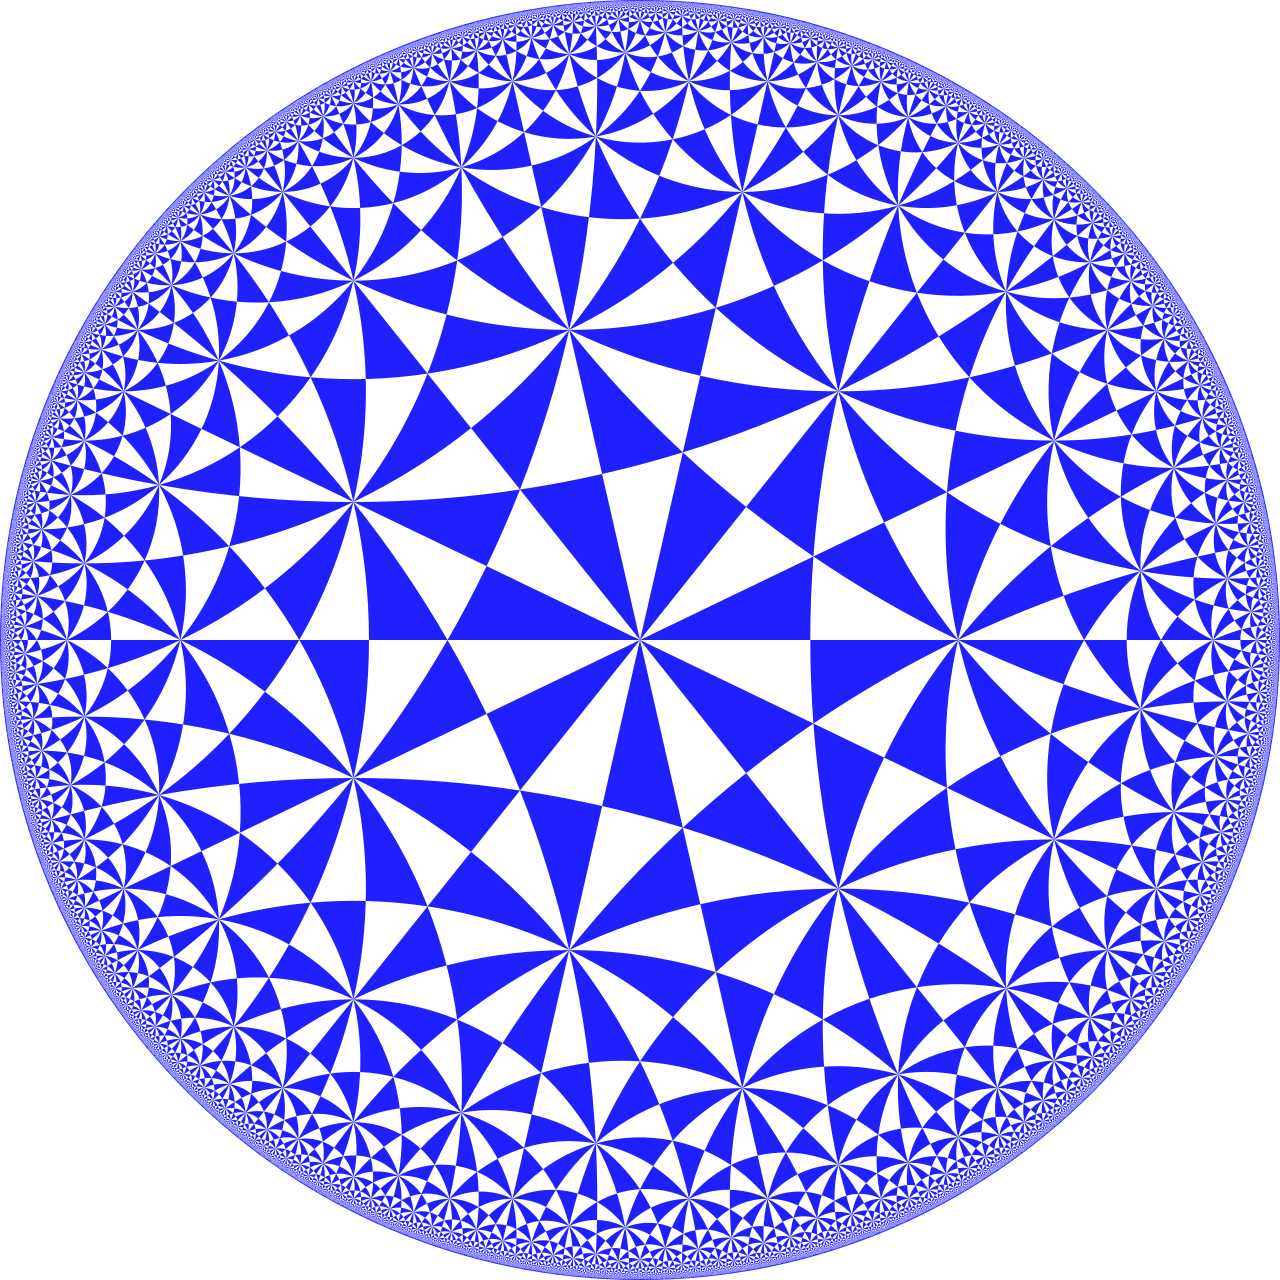
\includegraphics[width=.7\textwidth]{7-fold.png} %% 
      \end{center}
    \end{column}
  \end{columns}
  
\end{frame}

%%====================================================================

\begin{frame}{A simply transitive action of $\PSL_2(\Z)$} \smallskip
  
  The projective special linear group \vspace{-1mm}
  \[
  \PSL_2(\Z)=\SL_2(\Z)/\<-I\>,\qquad\text{where\; $\SL_2(\Z)=\Bigg\<
    \underbrace{\Balert{\begin{bmatrix}0 & -1 \\ 1 & 0\end{bmatrix}}}_S,\;
    \underbrace{\Alert{\begin{bmatrix}1 & 1 \\ 0 & 1\end{bmatrix}}}_T$}\Bigg\>
  \]
  \vspace{-2mm}
  
  defines a tiling of hyperbolic ideal triangles in the upper half-plane via
  \[
  \Balert{S}\colon z\longmapsto\frac{0z-1}{z+0}=-\frac{1}{z},\qquad\text{and}\qquad 
  \Alert{T}\colon z\longmapsto \frac{z+1}{0z+1}=z+1,
  \]
  
  %% PSL_2(Z) acting on hyperbolic ideal triangles
  \[
  \begin{tikzpicture}[scale=2.4]
    \tikzstyle{v0} = [circle, draw, fill=lightgray,inner sep=0pt, 
      minimum size=1.75mm]
    \tikzstyle{v1} = [circle, draw, fill=lightgray,inner sep=0pt, 
      minimum size=1.375mm]
    \tikzstyle{v2} = [circle, draw, fill=lightgray,inner sep=0pt, 
      minimum size=1mm]
    \tikzstyle{v3} = [circle, draw, fill=lightgray,inner sep=0pt, 
      minimum size=.75mm]
    \tikzstyle{v35} = [circle, draw, fill=lightgray,inner sep=0pt, 
      minimum size=.675mm]
    \tikzstyle{v4} = [circle, draw, fill=lightgray,inner sep=0pt, 
      minimum size=.725mm]
    \tikzstyle{v5} = [circle, draw, fill=lightgray,inner sep=0pt, 
      minimum size=.5mm]
    \tikzstyle{v6} = [circle, draw, fill=lightgray,inner sep=0pt, 
      minimum size=.45mm]
    %%
    \tikzstyle{r} = [draw, eRed, -stealth]
    \tikzstyle{bb} = [draw, eBlue]
    %%
    \tikzstyle{r-thin} = [draw, thin, eRed, -stealth]
    \tikzstyle{bb-thin} = [draw, eBlue]
    %%
    \draw [white] (-.5,1.75) -- (.5,1.75);
    \draw [white,fill=white] (1,0) arc(0:180:1) -- cycle;
    \draw[faded] (1,0) arc(0:180:1);
    \draw [dashed] (-2.0,0) -- (2.0,0);
    \draw[faded]  (-1.5,0) -- (-1.5,1.75);
    \draw[faded]  (-.5,0) -- (-.5,1.75);
    \draw[faded]  (.5,0) -- (.5,1.75);
    \draw[faded]  (1.5,0) -- (1.5,1.75);
    \draw[faded] (-2,0) arc(0:45:1);
    \draw[faded] (0,0) arc(0:180:1);
    \draw[faded] (2,0) arc(0:180:1);
    \draw[faded] (-1,0) arc(0:105:1);
    \draw[faded] (1,0) arc(180:75:1);
    \draw[faded] (2,0) arc(180:135:1);
    %%
    \draw[faded] (-2,0) -- (-2,-.065);
    \draw[faded] (-1.5,0) -- (-1.5,-.05);
    \draw[faded] (-1,0) -- (-1,-.065);
    \draw[faded] (-.5,0) -- (-.5,-.05);
    \draw[faded] (0,0) -- (0,-.065);
    \draw[faded] (.5,0) -- (.5,-.05);
    \draw[faded] (1,0) -- (1,-.065);
    \draw[faded] (1.5,0) -- (1.5,-.05);
    \draw[faded] (2,0) -- (2,-.065);
    %%
    \node at (-2,-.12) {\scriptsize $-2$};
    \node at (-1.5,-.12) {\tiny $-\frac{3}{2}$};
    \node at (-1,-.12) {\scriptsize $-1$};
    \node at (-.5,-.12) {\tiny $-\frac{1}{2}$};
    \node at (0,-.12) {\scriptsize $0$};
    \node at (.5,-.12) {\tiny $\frac{1}{2}$};    
    \node at (1,-.12) {\scriptsize $1$};
    \node at (1.5,-.12) {\tiny $\frac{3}{2}$};    
    \node at (2,-.12) {\scriptsize $2$};
    %%
    \draw[faded] (-2,0) arc(0:80:.333);
    \draw[faded] (-2,0) arc(0:115:.201);
    \draw[faded] (-2,0) arc(0:150:.141);
    \draw[white,fill=white] (-2.25,0) rectangle (-2.3,1.1);
    \draw[faded] (2,0) arc(180:100:.333);
    \draw[faded] (2,0) arc(180:65:.201);
    \draw[faded] (2,0) arc(180:30:.141);
    \draw[white,fill=white] (2.25,0) rectangle (2.3,1.1);
    \draw[faded] (-2,0) arc(180:0:.1);
    \draw[faded] (-2,0) arc(0:180:.1);
    %%
    \draw[faded] (-2,0) arc(180:0:.333);
    \draw[faded] (-1,0) arc(0:180:.333);
    \draw[faded] (-2,0) arc(180:0:.201);
    \draw[faded] (-1,0) arc(0:180:.201);
    \draw[faded] (-1.5,0) arc(0:180:.127);
    \draw[faded] (-1.5,0) arc(180:0:.127);
    \draw[faded] (-2,0) arc(180:0:.141);
    \draw[faded] (-1,0) arc(0:180:.141);
    \draw[faded] (-1,0) arc(180:0:.1);
    \draw[faded] (-1,0) arc(0:180:.1);
    \draw[faded] (-1,0) arc(180:0:.1);
    \draw[faded] (-1,0) arc(0:180:.1);
    %%
    \draw[faded] (-1,0) arc(180:0:.333);
    \draw[faded] (0,0) arc(0:180:.333);
    \draw[faded] (-1,0) arc(180:0:.201);
    \draw[faded] (0,0) arc(0:180:.201);
    \draw[faded] (-.5,0) arc(0:180:.127);
    \draw[faded] (-.5,0) arc(180:0:.127);
    \draw[faded] (-1,0) arc(180:0:.141);
    \draw[faded] (0,0) arc(0:180:.141);
    \draw[faded] (0,0) arc(180:0:.1);
    \draw[faded] (0,0) arc(0:180:.1);
    %%
    \draw[faded] (0,0) arc(180:0:.333);
    \draw[faded] (1,0) arc(0:180:.333);
    \draw[faded] (0,0) arc(180:0:.201);
    \draw[faded] (1,0) arc(0:180:.201);
    \draw[faded] (.5,0) arc(0:180:.127);
    \draw[faded] (.5,0) arc(180:0:.127);
    \draw[faded] (0,0) arc(180:0:.141);
    \draw[faded] (1,0) arc(0:180:.141);
    \draw[faded] (1,0) arc(180:0:.1);
    \draw[faded] (1,0) arc(0:180:.1);
    %%
    \draw[faded] (1,0) arc(180:0:.333);
    \draw[faded] (2,0) arc(0:180:.333);
    \draw[faded] (1,0) arc(180:0:.201);
    \draw[faded] (2,0) arc(0:180:.201);
    \draw[faded] (1.5,0) arc(0:180:.127);
    \draw[faded] (1.5,0) arc(180:0:.127);
    \draw[faded] (1,0) arc(180:0:.141);
    \draw[faded] (2,0) arc(0:180:.141);
    \draw[faded] (2,0) arc(180:0:.1);
    \draw[faded] (2,0) arc(0:180:.1);
    %%
    \node (T-3) at (-2.25,1.5) {};
    \node (T-2) at (-2,1.5) [v0] {};
    \node (T-1) at (-1,1.5)  [v0] {};
    \node (I) at (0,1.5) [v0] {};
    \node (T) at (1,1.5) [v0] {};
    \node (T2) at (2,1.5) [v0] {};
    \node (T3) at (2.25,1.5) {};
    \draw [r] (T-3) to (T-2) {};
    \draw [r] (T-2) to (T-1) {};
    \draw [r] (T-1) to (I) {};
    \draw [r] (I) to (T) {};
    \draw [r] (T) to (T2) {};
    \draw [r] (T2) to (T3) {};
    %%
    \node (T-2S) at (-2,.78) [v1] {};
    \node (T-1S) at (-1,.78) [v1] {};
    \node (S) at (0,.78) [v1] {};
    \node (TS) at (1,.78) [v1] {};
    \node (T2S) at (2,.78) [v1] {};
    \draw [bb] (T-2) to (T-2S);
    \draw [bb] (T-1) to (T-1S);
    \draw [bb] (I) to (S);
    \draw [bb] (T) to (TS);
    \draw [bb] (T2) to (T2S);
    %%
    \node (T-2ST) at (-2.3,.44) [v2] {};
    \node (T-2ST-1) at (-1.7,.44) [v2] {};
    \node (T-1ST) at (-1.3,.44) [v2] {};
    \node (T-1ST-1) at (-.7,.44) [v2] {};
    \node (ST) at (-.3,.44) [v2] {};
    \node (ST-1) at (.3,.44) [v2] {};
    \node (TST) at (.7,.44) [v2] {};
    \node (TST-1) at (1.3,.44) [v2] {};
    \node (T2ST) at (1.7,.44) [v2] {};
    \node (T2ST-1) at (2.3,.44) [v2] {};
    %%
    \node (T-2ST2) at (-2.3,.25) [v3] {};
    \node (T-2ST-2) at (-1.7,.25) [v3] {};
    \node (T-1ST2) at (-1.3,.25) [v3] {};
    \node (T-1ST-2) at (-.7,.25) [v3] {};
    \node (ST2) at (-.3,.25) [v3] {};
    \node (ST-2) at (.3,.25) [v3] {};    
    \node (TST2) at (.7,.25) [v3] {};
    \node (TST-2) at (1.3,.25) [v3] {};
    \node (T2ST2) at (1.7,.25) [v3] {};
    \node (T2ST-2) at (2.3,.25) [v3] {};
    %%
    \node (T-2ST3) at (-2.25,.15) [v4] {};
    \node (T-2ST-3) at (-1.75,.15) [v4] {};
    \node (T-1ST3) at (-1.25,.15) [v4] {};
    \node (T-1ST-3) at (-.75,.15) [v4] {};
    \node (ST3) at (-.25,.15) [v4] {};
    \node (ST-3) at (.25,.15) [v4] {};    
    \node (TST3) at (.75,.15) [v4] {};
    \node (TST-3) at (1.25,.15) [v4] {};
    \node (T2ST3) at (1.75,.15) [v4] {};
    \node (T2ST-3) at (2.25,.15) [v4] {};
    %%
    \node (T-2ST4) at (-2.18,.10) [v5] {};
    \node (T-2ST-4) at (-1.82,.10) [v5] {};
    \node (T-1ST4) at (-1.18,.10) [v5] {};
    \node (T-1ST-4) at (-.82,.10) [v5] {};
    \node (ST4) at (-.18,.10) [v5] {};
    \node (ST-4) at (.18,.10) [v5] {};    
    \node (TST4) at (.82,.10) [v5] {};
    \node (TST-4) at (1.18,.10) [v5] {};
    \node (T2ST4) at (1.82,.10) [v5] {};
    \node (T2ST-4) at (2.18,.10) [v5] {};  
    %%
    \draw [r] (T2ST-4) to (T2ST-3) {};
    \draw [r] (T2ST-3) to (T2ST-2) {};
    \draw [r] (T2ST-2) to (T2ST-1) {};
    \draw [r] (T2ST-1) to (T2S) {};
    \draw [r] (T2S) to (T2ST) {};
    \draw [r] (T2ST) to (T2ST2) {};
    \draw [r] (T2ST2) to (T2ST3) {};
    \draw [r] (T2ST3) to (T2ST4) {};
    %%
    \draw [r] (TST-4) to (TST-3) {};
    \draw [r] (TST-3) to (TST-2) {};
    \draw [r] (TST-2) to (TST-1) {};
    \draw [r] (TST-1) to (TS) {};
    \draw [r] (TS) to (TST) {};
    \draw [r] (TST) to (TST2) {};
    \draw [r] (TST2) to (TST3) {};
    \draw [r] (TST3) to (TST4) {};    
    %%
    \draw [r] (ST-4) to (ST-3) {};
    \draw [r] (ST-3) to (ST-2) {};
    \draw [r] (ST-2) to (ST-1) {};
    \draw [r] (ST-1) to (S) {};
    \draw [r] (S) to (ST) {};
    \draw [r] (ST) to (ST2) {};
    \draw [r] (ST2) to (ST3) {};
    \draw [r] (ST3) to (ST4) {};        
    %%
    \draw [r] (T-1ST-4) to (T-1ST-3) {};
    \draw [r] (T-1ST-3) to (T-1ST-2) {};
    \draw [r] (T-1ST-2) to (T-1ST-1) {};
    \draw [r] (T-1ST-1) to (T-1S) {};
    \draw [r] (T-1S) to (T-1ST) {};
    \draw [r] (T-1ST) to (T-1ST2) {};
    \draw [r] (T-1ST2) to (T-1ST3) {};
    \draw [r] (T-1ST3) to (T-1ST4) {};            
    %%
    \draw [r] (T-2ST-4) to (T-2ST-3) {};
    \draw [r] (T-2ST-3) to (T-2ST-2) {};
    \draw [r] (T-2ST-2) to (T-2ST-1) {};
    \draw [r] (T-2ST-1) to (T-2S) {};
    \draw [r] (T-2S) to (T-2ST) {};
    \draw [r] (T-2ST) to (T-2ST2) {};
    \draw [r] (T-2ST2) to (T-2ST3) {};
    \draw [r] (T-2ST3) to (T-2ST4) {};            
    %%
    \draw [bb] (T-2ST-1) to (T-1ST) {};
    \draw [bb] (T-1ST-1) to (ST) {};
    \draw [bb] (ST-1) to (TST) {};
    \draw [bb] (TST-1) to (T2ST) {};
    %%
    \node [v35] (T-2ST-2S) at (-1.57,.17) {};
    \node [v35] (T-1ST2S) at (-1.43,.17) {};
    \draw [r] (T-1ST2S) to (T-2ST-2S);
    \draw [bb] (T-2ST-2S) to (T-2ST-2);
    \draw [bb] (T-1ST2) to (T-1ST2S);
    %%
    \node [v35] (T-1ST-2S) at (-.57,.17) {};
    \node [v35] (ST2S) at (-.43,.17) {};
    \draw [r] (ST2S) to (T-1ST-2S);
    \draw [bb] (T-1ST-2S) to (T-1ST-2);
    \draw [bb] (ST2) to (ST2S);
    %%
    \node [v35] (ST-2S) at (.43,.17) {};
    \node [v35] (TST2S) at (.57,.17) {};
    \draw [r] (TST2S) to (ST-2S);
    \draw [bb] (ST-2S) to (ST-2);
    \draw [bb] (TST2) to (TST2S);
%%
    \node [v35] (TST-2S) at (1.43,.17) {};
    \node [v35] (T2ST2S) at (1.57,.17) {};
    \draw [r] (T2ST2S) to (TST-2S);
    \draw [bb] (TST-2S) to (TST-2);
    \draw [bb] (T2ST2) to (T2ST2S);
    %%
    \node [v6] (-2L_R) at (-2.31,.08) {};
    \node [v6] (-2R_L) at (-1.69,.08) {}; \node [v6] (-2R_M) at (-1.635,.07) {};
    \node [v6] (-2R_R) at (-1.58,.09) {}; \node [v6] (-1R_L) at (-.69,.08) {};
    \node [v6] (-1R_M) at (-.635,.07) {}; \node [v6] (-1R_R) at (-.58,.09) {};
    \node [v6] (0R_L) at (.31,.08) {}; \node [v6] (0R_M) at (.365,.07) {};
    \node [v6] (0R_R) at (.42,.09) {}; \node [v6] (1R_L) at (1.31,.08) {};
    \node [v6] (1R_M) at (1.365,.07) {}; \node [v6] (1R_R) at (1.42,.09) {};
    \node [v6] (-1L_R) at (-1.31,.08) {}; \node [v6] (-1L_M) at (-1.365,.07) {};
    \node [v6] (-1L_L) at (-1.42,.09) {}; \node [v6] (0L_R) at (-.31,.08) {};
    \node [v6] (0L_M) at (-.365,.07) {}; \node [v6] (0L_L) at (-.42,.09) {};
    \node [v6] (1L_R) at (.69,.08) {}; \node [v6] (1L_M) at (.635,.07) {};
    \node [v6] (1L_L) at (.58,.09) {}; \node [v6] (2L_R) at (1.69,.08) {};
    \node [v6] (2L_M) at (1.635,.07) {}; \node [v6] (2L_L) at (1.58,.09) {};
    \node [v6] (2R_L) at (2.31,.08) {};
    %%
    \draw [r-thin] (T-2ST-2S) to (-2R_R); \draw [bb-thin] (-2R_R) to (-2R_M);
    \draw [r-thin] (-2R_M) to (-2R_L); \draw [bb-thin] (T-2ST-3) to (-2R_L); 
    \draw [r-thin] (T-1ST-2S) to (-1R_R); \draw [bb-thin] (-1R_R) to (-1R_M);
    \draw [r-thin] (-1R_M) to (-1R_L); \draw [bb-thin] (T-1ST-3) to (-1R_L);
    \draw [r-thin] (ST-2S) to (0R_R); \draw [bb-thin] (0R_R) to (0R_M);
    \draw [r-thin] (0R_M) to (0R_L); \draw [bb-thin] (ST-3) to (0R_L);
    \draw [r-thin] (TST-2S) to (1R_R); \draw [bb-thin] (1R_R) to (1R_M);
    \draw [r-thin] (1R_M) to (1R_L); \draw [bb-thin] (TST-3) to (1R_L);
    %%
    \draw [bb-thin] (T-1ST3) to (-1L_R); \draw [r-thin] (-1L_R) to (-1L_M);
    \draw [bb-thin] (-1L_M) to (-1L_L); \draw [r-thin] (-1L_L) to (T-1ST2S);
    \draw [bb-thin] (ST3) to (0L_R); \draw [r-thin] (0L_R) to (0L_M);
    \draw [bb-thin] (0L_M) to (0L_L); \draw [r-thin] (0L_L) to (ST2S);
    \draw [bb-thin] (TST3) to (1L_R); \draw [r-thin] (1L_R) to (1L_M);
    \draw [bb-thin] (1L_M) to (1L_L); \draw [r-thin] (1L_L) to (TST2S);
    \draw [bb-thin] (T2ST3) to (2L_R); \draw [r-thin] (2L_R) to (2L_M);
    \draw [bb-thin] (2L_M) to (2L_L); \draw [r-thin] (2L_L) to (T2ST2S);
    %%
    \draw [bb-thin] (T-2ST3) to (-2L_R); \draw [bb-thin] (T2ST-3) to (2R_L);
  \end{tikzpicture}
  \]
  
\end{frame}

%%====================================================================

\begin{frame}[fragile]{Equivariance and morphisms of $G$-sets}
  
  \begin{alertblock}{Key idea}
    \begin{itemize}
    \item \Alert{Action equivalence} involves an isomorphism
      $\iota\colon G_1\to G_2$ and bijection $\sigma\colon S_1\to
      S_2$.
    \item \Alert{Equivariant bijections} ($\iota=\Id$) define
      \Balert{$G$-set isomorphisms}.
    \item \Alert{Equivariant maps} ($\iota=\Id$, but $\sigma$
      need not be bijective) define \Balert{$G$-set homomorphisms}.
    \end{itemize}
  \end{alertblock}

  \begin{block}{Definition}
    Suppose $G$ acts on $S_i$ via $\phi_i\colon G\to\Perm(S_i)$ for
    $i=1,2$. A \Alert{\textbf{$G$-equivariant map}} is a function
    $\sigma\colon S_1\to S_2$ such that
    $\sigma\circ\phi_1(g)=\phi_2(g)\circ\sigma$, for all $g\in G$:
    %%
    %% Commutative diagrams of G-equivarent maps
    \[
    \begin{tikzpicture}[scale=1.3,xscale=1.5,
        baseline=(current bounding box.center)]]
        \begin{scope}[shift={(0,0)}]
          \node (NW) at (0,1) {$S_1$};
          \node (NE) at (1,1) {$S_1$};
          \node (SW) at (0,0) {$S_2$};
          \node (SE) at (1,0) {$S_2$};
          \draw[|->] (NW) -- (NE) node[midway,above]{\footnotesize $\phi_1(g)$};
          \draw[|->] (NW) -- (SW) node[midway,left]{\footnotesize $\sigma$};
          \draw[|->] (NE) -- (SE) node[midway,right]{\footnotesize $\sigma$};
          \draw[|->] (SW) -- (SE) node[midway,above]{\footnotesize $\phi_2(g)$};
        \end{scope}
        %%
        \begin{scope}[shift={(2.5,0)}]
          \node (NW) at (0,1) {$s_1$}; \node (NE) at (1,1) {$s_1\Dot\phi_1(g)$};
          \node (SW) at (0,0) {$s_2$}; \node (SE) at (1,0) {$s_2\Dot\phi_2(g)$};
          \draw[|->] (NW) -- (NE) node[midway,above]{\footnotesize $\phi_1(g)$};
          \draw[|->] (NW) -- (SW) node[midway,left]{\footnotesize $\sigma$};
          \draw[|->] (NE) -- (SE) node[midway,right]{\footnotesize $\sigma$};
          \draw[|->] (SW) -- (SE) node[midway,above]{\footnotesize $\phi_2(g)$};
        \end{scope}
        %%
    \end{tikzpicture}
    \]
  \end{block}
  
  \medskip
  
  Special cases:
  \begin{itemize}
  \item Equivariant bijection (\Balert{$G$-set isomorphism}): when
    $\sigma$ is bijective.
  \item If $S:=S_1=S_2$, then we get the group $\Aut_G(S)$ of \Balert{$G$-set
    automorphisms.}
  \end{itemize}   

\end{frame}

%%====================================================================

\begin{frame}{Equivalence of actions vs.\ $G$-set isomorphism} %\vspace{-2mm}

  The following actions are equivalent, via $\omega\in\Aut(D_4)$,
  where $f\mapsto rf$,
  %%
  %%
  %% Picture of an action equivalence of G-sets that isn't an isomorphism
  \[
  \begin{tikzpicture}[scale=.65,auto]
    \draw[-stealth,very thick] (2,1.25) to node[above] {\small $\bm{\sigma}$} (4.25,1.25);
    \tikzstyle{every node}=[font=\footnotesize]
    %%
    %% Picture of an square with blue and green axes.
    %%
    \begin{scope}[shift={(-4.5,-.25)},scale=.75]
      \tikzstyle{every node}=[font=\normalsize]
      \draw [dashed,ultra thick,eBlue] (.5,-.8) to (.5,1.8);
      \draw [dashed,ultra thick,eGreen] (-.75,-.75) to (1.75,1.75);
      \draw (0,0) rectangle (1,1);
      \node at (.5,2.35) {$\color{xBlue}f$};
      \node at (2.05,2.15) {$\color{xGreen}rf$};
    \end{scope}
    %%
    %% Picture of an square with blue and green axes, but rotated 45 degrees
    %%
    \begin{scope}[shift={(10,-.25)},scale=.75]
      \tikzstyle{every node}=[font=\normalsize]
      \draw [dashed,very thick,eGreen] (-.8,.5) to (1.8,.5);
      \draw [dashed,ultra thick,eBlue] (-.75,-.75) to (1.75,1.75);
      \draw (0,0) rectangle (1,1);
      \node at (2.05,2.1) {$\color{xBlue}rf\!=\!\omega(f)$};
      \node at (2.25,-.35) {$\color{xGreen}r^2\!f\!=\!\omega(rf)$};
    \end{scope}
    %%
    %% First binary square size-4 orbit (blue and green arrows)
    %%
    \begin{scope}[shift={(0,0)},shorten >= 0pt, shorten <= 0pt,scale=.7]
            \tikzstyle{every node}=[font=\scriptsize]
      %%
      \begin{scope}[shift={(1.95,0)}]  %% H
        \path[fill=actOrange] (-.5,0) rectangle ++(.5,.5); 
        \path[fill=actOrange] (0,0) rectangle ++(.5,.5);
        \path[fill=actPurple] (-.5,-.5) rectangle ++(.5,.5);
        \path[fill=actPurple] (0,-.5) rectangle ++(.5,.5);
        \draw (-.5,-.5) rectangle (.5,.5);
        \draw (-.25,.25) node{$0$}; \draw (.25,.25) node{$0$};
        \draw (-.25,-.25) node{$1$}; \draw (.25,-.25) node{$1$};
        \node (0-out) at (0,.5) {};
        \node (0-in) at (0,-.5) {};
        \node (0-gg) at (-.5,-.25) {};
        \Loop[dist=1.5cm,dir=EA,color=eBlue](.5,0);
      \end{scope}
      %%
      \begin{scope}[shift={(0,1.95)}] %% Hr
        \path[fill=actOrange] (-.5,0) rectangle ++(.5,.5); 
        \path[fill=actPurple] (0,0) rectangle ++(.5,.5);
        \path[fill=actOrange] (-.5,-.5) rectangle ++(.5,.5);
        \path[fill=actPurple] (0,-.5) rectangle ++(.5,.5);
        \draw (-.5,-.5) rectangle (.5,.5);
        \draw (-.25,.25) node{$0$}; \draw (.25,.25) node{$1$};
        \draw (-.25,-.25) node{$0$}; \draw (.25,-.25) node{$1$};
        \node (90-out) at (-.5,0) {};
        \node (90-in) at (.5,0) {};
        \node (90-bb) at (0,-.5) {};
        \node (90-gg) at (-.25,-.5) {};
      \end{scope}
      %%
      \begin{scope}[shift={(-1.95,0)}] %% Hr^2
        \path[fill=actPurple] (-.5,0) rectangle ++(.5,.5); 
        \path[fill=actPurple] (0,0) rectangle ++(.5,.5);
        \path[fill=actOrange] (-.5,-.5) rectangle ++(.5,.5);
        \path[fill=actOrange] (0,-.5) rectangle ++(.5,.5);
        \draw (-.5,-.5) rectangle (.5,.5);
        \draw (-.25,.25) node{$1$}; \draw (.25,.25) node{$1$};
        \draw (-.25,-.25) node{$0$}; \draw (.25,-.25) node{$0$};
        \Loop[dist=1.5cm,dir=WE,color=eBlue](-.5,0);
        \node (180-out) at (0,-.5) {};
        \node (180-in) at (0,.5) {};
        \node (180-gg) at (.5,.25) {};
      \end{scope}
      %%
      \begin{scope}[shift={(0,-1.95)}] %% Hr^3
        \path[fill=actPurple] (-.5,0) rectangle ++(.5,.5); 
        \path[fill=actOrange] (0,0) rectangle ++(.5,.5);
        \path[fill=actPurple] (-.5,-.5) rectangle ++(.5,.5);
        \path[fill=actOrange] (0,-.5) rectangle ++(.5,.5);
        \draw (-.5,-.5) rectangle (.5,.5);
        \draw (-.25,.25) node{$1$}; \draw (.25,.25) node{$0$};
        \draw (-.25,-.25) node{$1$}; \draw (.25,-.25) node{$0$};        
        \node (270-out) at (.5,0) {};
        \node (270-in) at (-.5,0) {};
        \node (270-bb) at (0,.5) {};
        \node (270-gg) at (.25,.5) {};
      \end{scope}
      %%
      \draw [r,shorten >= -2pt, shorten <= -2pt] (0-out)
      to [bend right=25] (90-in);
      \draw [r,shorten >= -2pt, shorten <= -2pt] (90-out)
      to [bend right=25] (180-in);
      \draw [r,shorten >= -2pt, shorten <= -2pt] (180-out)
      to [bend right=25] (270-in);
      \draw [r,shorten >= -2pt, shorten <= -2pt] (270-out)
      to [bend right=25] (0-in);
      \draw [bb,shorten >= -3pt, shorten <= -3pt] (90-bb) to (270-bb);
      \draw [gg,shorten >= -4pt, shorten <= -4pt] (0-gg) to (270-gg); 
      \draw [gg,shorten >= -4pt, shorten <= -4pt] (180-gg) to (90-gg);
    \end{scope} %% end of the 1st binary square example
    %%
    %% Second binary square size-4 orbit (colors blue and green swapped)
    %%
    \begin{scope}[shift={(6,0)},shorten >= 0pt, shorten <= 0pt,scale=.7]
     \tikzstyle{every node}=[font=\scriptsize]
      %%
      \begin{scope}[shift={(1.95,0)}]  %% H
        \path[fill=actOrange] (0,0)--(.5,.5)--(.5,-.5);
        \path[fill=actOrange] (0,0)--(-.5,.5)--(.5,.5);
        \path[fill=actPurple] (0,0)--(-.5,-.5)--(-.5,.5);
        \path[fill=actPurple] (0,0)--(-.5,-.5)--(.5,-.5);
        \draw (0,.28) node{$0$}; 
        \draw (-.32,0) node{$1$}; \draw (.32,.0) node{$0$}; 
        \draw (0,-.28) node{$1$};
        \draw (-.5,-.5) rectangle (.5,.5);
        \node (0-out) at (0,.5) {};
        \node (0-in) at (0,-.5) {};
        \node (0-pp) at (-.5,-.25) {};
        \Loop[dist=1.5cm,dir=EA,color=eBlue](.5,0);
      \end{scope}
      %%
      \begin{scope}[shift={(0,1.95)}] %% Hr
        \path[fill=actPurple] (0,0)--(.5,.5)--(.5,-.5);
        \path[fill=actOrange] (0,0)--(-.5,.5)--(.5,.5);
        \path[fill=actOrange] (0,0)--(-.5,-.5)--(-.5,.5);
        \path[fill=actPurple] (0,0)--(-.5,-.5)--(.5,-.5);
        \draw (0,.28) node{$0$}; 
        \draw (-.32,0) node{$0$}; \draw (.32,.0) node{$1$}; 
        \draw (0,-.28) node{$1$};
        \draw (-.5,-.5) rectangle (.5,.5);
        \node (90-out) at (-.5,0) {};
        \node (90-in) at (.5,0) {};
        \node (90-gg) at (0,-.5) {};
        \node (90-pp) at (-.25,-.5) {};
      \end{scope}
      %%
      \begin{scope}[shift={(-1.95,0)}] %% Hr^2
        \path[fill=actPurple] (0,0)--(.5,.5)--(.5,-.5);
        \path[fill=actPurple] (0,0)--(-.5,.5)--(.5,.5);
        \path[fill=actOrange] (0,0)--(-.5,-.5)--(-.5,.5);
        \path[fill=actOrange] (0,0)--(-.5,-.5)--(.5,-.5);
        \draw (0,.28) node{$1$}; 
        \draw (-.32,0) node{$0$}; \draw (.32,.0) node{$1$}; 
        \draw (0,-.28) node{$0$};
        \draw (-.5,-.5) rectangle (.5,.5);
        \Loop[dist=1.5cm,dir=WE,color=eBlue](-.5,0);
        \node (180-out) at (0,-.5) {};
        \node (180-in) at (0,.5) {};
        \node (180-pp) at (.5,.25) {};
      \end{scope}
      %%
      \begin{scope}[shift={(0,-1.95)}] %% Hr^3
        \path[fill=actOrange] (0,0)--(.5,.5)--(.5,-.5);
        \path[fill=actPurple] (0,0)--(-.5,.5)--(.5,.5);
        \path[fill=actPurple] (0,0)--(-.5,-.5)--(-.5,.5);
        \path[fill=actOrange] (0,0)--(-.5,-.5)--(.5,-.5);
        \draw (0,.28) node{$1$}; 
        \draw (-.32,0) node{$1$}; \draw (.32,.0) node{$0$}; 
        \draw (0,-.28) node{$0$};
        \draw (-.5,-.5) rectangle (.5,.5);
        \node (270-out) at (.5,0) {};
        \node (270-in) at (-.5,0) {};
        \node (270-gg) at (0,.5) {};
        \node (270-pp) at (.25,.5) {};
      \end{scope}
      %%
      \draw [r,shorten >= -2pt, shorten <= -2pt] (0-out)
      to [bend right=25] (90-in);
      \draw [r,shorten >= -2pt, shorten <= -2pt] (90-out)
      to [bend right=25] (180-in);
      \draw [r,shorten >= -2pt, shorten <= -2pt] (180-out)
      to [bend right=25] (270-in);
      \draw [r,shorten >= -2pt, shorten <= -2pt] (270-out)
      to [bend right=25] (0-in);
      \draw [bb,shorten >= -3pt, shorten <= -3pt] (90-gg) to (270-gg);
      \draw [gg,shorten >= -4pt, shorten <= -4pt] (0-pp) to (270-pp); 
      \draw [gg,shorten >= -4pt, shorten <= -4pt] (90-pp) to (180-pp);
    \end{scope}     
  \end{tikzpicture}
  \]
  \pause However, the corresponding $G$-sets are non-isomorphic.
  \[
  \begin{tikzpicture}[scale=.5]
    \begin{scope}[shift={(0,0)}]
      \tikzstyle{every node}=[font=\scriptsize]
      \node at (-1.45,.5) {\normalsize $H=\stab\!\Big($};
      \path[fill=actOrange] (0,.5) rectangle ++(.5,.5); 
      \path[fill=actOrange] (.5,.5) rectangle ++(.5,.5);
      \path[fill=actPurple] (0,0) rectangle ++(.5,.5);
      \path[fill=actPurple] (.5,0) rectangle ++(.5,.5);
      \draw (0,0) rectangle (1,1);
      \draw (.25,.75) node{$0$};\draw(.75,.75)node{$0$};
      \draw (.25,.25) node{$1$};\draw(.75,.25)node{$1$};
      \node at (2.15,.5) {\normalsize $\Big)=\<f\>$,};      
    \end{scope}
    %%
    \begin{scope}[shift={(8,0)}]
      \tikzstyle{every node}=[font=\scriptsize]
      \node at (-1.45,.5) {\normalsize $K=\stab\!\Big($};
      \path[fill=actOrange] (.5,.5)--(1,1)--(1,0);
      \path[fill=actOrange] (.5,.5)--(0,1)--(1,1);
      \path[fill=actPurple] (.5,.5)--(0,0)--(0,1);
      \path[fill=actPurple] (.5,.5)--(0,0)--(1,0);
      \draw (.5,.78) node{$0$}; 
      \draw (.18,.5) node{$1$}; \draw (.82,.5) node{$0$}; 
      \draw (.5,.22) node{$1$};
      \draw (0,0) rectangle (1,1);
      \node at (2.25,.5) {\normalsize $\Big)=\<rf\>$.};
    \end{scope}
  \end{tikzpicture}
  \]
  %%
  %% Several action graphs of D_4-sets
  \[
  \begin{tikzpicture}[scale=.6]
    %%
    %% Picture of an square with blue and green axes.
    %%
    \begin{scope}[shift={(-7,-1.75)},scale=1]
      \tikzstyle{v} = [circle, draw, fill=lightgray,inner sep=0pt, 
        minimum size=4.95mm]
      \node at (.5,4) {\small \emph{``Switchboard''}};
      \tikzstyle{every node}=[font=\small]
      \draw [midgray,fill=vYellow!50,rounded corners] (-.5,-.5)
      rectangle ++(2,4); 
      \node at (0,3) [v] {$1$}; \node at (1,3) [v,fill=vBlue] {$f$};
      \node at (0,2) [v,fill=vRed] {$r$}; \node at (1,2) [v] {$rf$};
      \node at (0,1) [v] {$r^2$}; \node at (1,1) [v] {$r^2\!f$};
      \node at (0,0) [v] {$r^3$}; \node at (1,0) [v] {$r^3\!f$};
    \end{scope}
    %%
    %% A size-4 orbit with unlabeled nodes
    %%
    \begin{scope}[shift={(0,0)},scale=1.75]
      \tikzstyle{R} = [draw, very thick, eRed,-stealth,bend right=28]
      \tikzstyle{v} = [circle, draw, fill=lightgray,inner sep=0pt,
        minimum size=4.5mm] 
      \tikzset{every loop/.style={min distance=5mm,looseness=12}}
      %%
      \node (1) at (0:1) [v] {$H$};
      \node (r) at (90:1) [v] {$Hr$};
      \node (r2) at (180:1) [v] {\small $Hr^2$};
      \node (r3) at (270:1) [v] {\small $Hr^3$};
      \draw[bb] (r) to (r3);
      \draw [R] (1) to (r); \draw[R]  (r) to (r2);
      \draw [R] (r2) to (r3); \draw[R]  (r3) to (1);
      \path (1) edge [b,loop right,-stealth] (1);
      \path (r2) edge [b,loop left,-stealth] (r2);
    \end{scope}
    %%
    %% A different size-4 orbit with unlabeled nodes
    %% 
    \begin{scope}[shift={(7,0)},scale=1.75]
    \tikzstyle{R} = [draw, very thick, eRed,-stealth,bend right=28]
    \tikzstyle{v} = [circle, draw, fill=lightgray,inner sep=0pt,
      minimum size=4.5mm] 
    \tikzset{every loop/.style={min distance=6mm,looseness=30}}
    %%
    \node (1) at (0:1) [v] {$K$};
    \node (r) at (90:1) [v] {$Kr$};
    \node (r2) at (180:1) [v] {\small $Kr^2$};
    \node (r3) at (270:1) [v] {\small $Kr^3$};
    \draw[bb] (1) to (r); \draw[bb] (r2) to (r3);
    \draw [R] (1) to (r); \draw[R]  (r) to (r2);
    \draw [R] (r2) to (r3); \draw[R]  (r3) to (1);
    \end{scope}
  \end{tikzpicture}
  \]
  
\end{frame}

%%====================================================================

\begin{frame}{$G$-set automorphisms as symmetries of the action graph}

  Let $S=G\!\setminus\!H$, for $G=D_6$ and $H=\<f\>$.
  %%
  %% Commutative diagrams of G-equivarent maps, with action graphs of D_6
  \[
  \tikzstyle{v-r} = [circle, draw, midgray, fill=cosetRed,inner sep=0pt, 
    minimum size=3.5mm]
  \tikzstyle{v-R} = [circle, draw, fill=vRed,inner sep=0pt, 
    minimum size=3.5mm]
  \tikzstyle{v-b} = [circle, draw, midgray, fill=cosetBlue,inner sep=0pt, 
    minimum size=3.5mm]
  \tikzstyle{v-B} = [circle, draw, fill=vBlue,inner sep=0pt, 
    minimum size=3.5mm]
  %%
  \tikzstyle{b-f} = [draw, ultra thick, cosetBlue,-stealth]
  \tikzstyle{bb-f} = [draw, ultra thick, cosetBlue]
  \tikzstyle{r-f} = [draw, very thick, eRed,-stealth,bend right=15]
  \tikzstyle{R-f} = [draw, ultra thick, cosetRed,-stealth,bend right=15]
  %%
  \begin{tikzpicture}[scale=.4]
    \tikzstyle{every node}=[font=\tiny]
    \tikzset{every loop/.style={min distance=10mm,looseness=20}}
    %%
    \begin{scope}[shift={(0,0)},scale=1]
      \node (H) at (0:2) [v-B] {\scriptsize $\bm{H}$};
      \node[midgray] (Hr) at (60:2) [v-r] {\scriptsize $Hr$};
      \node[midgray] (Hr2) at (120:2) [v-r] {$H\!r^2$};
      \node[midgray] (Hr3) at (180:2) [v-b] {$H\!r^3$};
      \node[midgray] (Hr4) at (240:2) [v-r] {$H\!r^4$};
      \node[midgray] (Hr5) at (300:2) [v-r] {$H\!r^5$};
      \path[R-f] (H) to (Hr);
      \path[R-f] (Hr) to (Hr2);
      \path[R-f] (Hr2) to (Hr3);
      \path[R-f] (Hr3) to (Hr4);
      \path[R-f] (Hr4) to (Hr5);
      \path[R-f] (Hr5) to (H);
      \path[bb-f] (Hr) to (Hr5);
      \path[bb-f] (Hr2) to (Hr4);
      \path (H) edge [b-f,loop right,>=stealth] (H);
      \path (Hr3) edge [b-f,loop left,>=stealth] (Hr3);
    \end{scope}
    %%
    \begin{scope}[shift={(0,-8)},scale=1]
      \node[midgray] (H) at (0:2) [v-b] {$H\!r^3$};
      \node[midgray] (Hr) at (60:2) [v-r] {$H\!r^4$};
      \node[midgray] (Hr2) at (120:2) [v-r] {$H\!r^5$};
      \node (Hr3) at (180:2) [v-B] {\scriptsize $\bm{H}$};
      \node[midgray] (Hr4) at (240:2) [v-r] {\scriptsize $H\!r$};
      \node[midgray] (Hr5) at (300:2) [v-r] {$H\!r^2$};
      \path[R-f] (H) to (Hr);
      \path[R-f] (Hr) to (Hr2);
      \path[R-f] (Hr2) to (Hr3);
      \path[R-f] (Hr3) to (Hr4);
      \path[R-f] (Hr4) to (Hr5);
      \path[R-f] (Hr5) to (H);
      \path[bb-f] (Hr) to (Hr5);
      \path[bb-f] (Hr2) to (Hr4);
      \path (H) edge [b-f,loop right,>=stealth] (H);
      \path (Hr3) edge [b-f,loop left,>=stealth] (Hr3);
    \end{scope}
    %%
    \begin{scope}[shift={(14,0)},scale=1]
      \node (H) at (0:2) [v-B] {\scriptsize $\bm{H}$};
      \node (Hr) at (60:2) [v-R] {\scriptsize $\bm{Hr}$};
      \node[midgray] (Hr2) at (120:2) [v-r] {$H\!r^2$};
      \node[midgray] (Hr3) at (180:2) [v-b] {$H\!r^3$};
      \node[midgray] (Hr4) at (240:2) [v-r] {$H\!r^4$};
      \node[midgray] (Hr5) at (300:2) [v-r] {$H\!r^5$};
      \path[r-f] (H) to (Hr);
      \path[R-f] (Hr) to (Hr2);
      \path[R-f] (Hr2) to (Hr3);
      \path[R-f] (Hr3) to (Hr4);
      \path[R-f] (Hr4) to (Hr5);
      \path[R-f] (Hr5) to (H);
      \path[bb-f] (Hr) to (Hr5);
      \path[bb-f] (Hr2) to (Hr4);
      \path (H) edge [b-f,loop right,>=stealth] (H);
      \path (Hr3) edge [b-f,loop left,>=stealth] (Hr3);
    \end{scope}
    %%      
    \begin{scope}[shift={(14,-8)},scale=1]
      \node[midgray] (H) at (0:2) [v-b] {$H\!r^3$};
      \node[midgray] (Hr) at (60:2) [v-r] {$H\!r^4$};
      \node[midgray] (Hr2) at (120:2) [v-r] {$H\!r^5$};
      \node (Hr3) at (180:2) [v-B] {\scriptsize $\bm{H}$};
      \node (Hr4) at (240:2) [v-R] {\scriptsize $\bm{Hr}$};
      \node[midgray] (Hr5) at (300:2) [v-r] {$H\!r^2$};
      \path[R-f] (H) to (Hr);
      \path[R-f] (Hr) to (Hr2);
      \path[R-f] (Hr2) to (Hr3);
      \path[r-f] (Hr3) to (Hr4);
      \path[R-f] (Hr4) to (Hr5);
      \path[R-f] (Hr5) to (H);
      \path[bb-f] (Hr) to (Hr5);
      \path[bb-f] (Hr2) to (Hr4);
      \path (H) edge [b-f,loop right,>=stealth] (H);
      \path (Hr3) edge [b-f,loop left,>=stealth] (Hr3);
    \end{scope}
    %%
    \draw [very thick,->] (4.25,0) -- (9.75,0)
    node[midway,above]{\normalsize $\phi(r)$};
    \draw [very thick,->] (4.25,-8) -- (9.75,-8)
    node[midway,above]{\normalsize $\phi(r)$};
    \draw [very thick,->] (0,-2.5) -- (0,-5.5)
    node[midway,left]{\normalsize $\sigma$}
    node[pos=.55, below right]{\small\emph{$180^\circ$ rotation}};
    \draw [very thick,->] (14,-2.5) -- (14,-5.5)
    node[pos=.55,below left]{\small\emph{$180^\circ$ rotation}}
    node[midway,right]{\normalsize $\sigma$};
  \end{tikzpicture}
  \]
  
  \vspace{-1mm}
  
  \begin{alertblock}{Key idea}
    The action and bijection clearly commute upon thinking of:
    \begin{itemize}
    \item the \Alert{action} $\phi(r)$ as \Alert{right-multiplying}
      $Hr^i$ by $r$,
    \item the \Balert{bijection} $\sigma$ as \Balert{left-multiplying}
      $Hr^i$ by $r^3$. (This works because $r^3\in N_G(H)$).
    \end{itemize}
  \end{alertblock}
  
\end{frame}

%%====================================================================

\begin{frame}{$G$-set automorphisms} \vspace{-8mm}

  %% Cayley graph and subgroup lattice of D_6.
  \[
  \begin{tikzpicture}[scale=.6]
    \newcommand\Hf{6.495} % height of C_12 
    \newcommand\He{5.196} % height of C_6  
    \newcommand\Hd{3.897} % height of C_4 
    \newcommand\Hc{2.598} % height of C_3  
    \newcommand\Hb{1.299} % height of C_2 
    \newcommand\Ha{0} % height of C_1   
    \tikzstyle{R6-out} = [draw, very thick, eRed,-stealth,bend right=18]
    \tikzstyle{R6-in} = [draw, very thick, eRed,-stealth,bend left=12]
    \tikzstyle{R-in} = [draw, very thick, eRed,-stealth,bend left=12]
    %%
    \begin{scope}[shift={(0,3.5)},scale=1.45]
      \tikzstyle{v} = [circle, draw, fill=lightgray,inner sep=0pt, 
        minimum size=3.5mm]
      \tikzstyle{R6-out} = [draw, very thick, eRed,-stealth,bend right=18]
      \tikzstyle{R6-in} = [draw, very thick, eRed,-stealth,bend left=12]
      \tikzstyle{every node}=[font=\footnotesize]
      \node (1) at (0:2) [v] {$1$};
      \node (r) at (60:2) [v] {$r$};
      \node (r2) at (120:2) [v] {$r^2$};
      \node (r3) at (180:2) [v] {$r^3$};
      \node (r4) at (240:2) [v] {$r^4$};
      \node (r5) at (300:2) [v] {$r^5$};
      \node (f) at (0:1) [v] {$f$};
      \node (rf) at (60:1) [v] {$rf$};
      \node (r2f) at (120:1) [v] {$r^2\!f$};
      \node (r3f) at (180:1) [v] {$r^3\!f$};
      \node (r4f) at (240:1) [v] {$r^4\!f$};
      \node (r5f) at (300:1) [v] {$r^5\!f$};
      \path[bb] (1) to (f);
      \path[bb] (r) to (rf);
      \path[bb] (r2) to (r2f);
      \path[bb] (r3) to (r3f);
      \path[bb] (r4) to (r4f);
      \path[bb] (r5) to (r5f);
      \path[R6-out] (1) to (r);
      \path[R6-out] (r) to (r2);
      \path[R6-out] (r2) to (r3);
      \path[R6-out] (r3) to (r4);
      \path[R6-out] (r4) to (r5);
      \path[R6-out] (r5) to (1);
      \path[R6-in] (f) to (r5f);
      \path[R6-in] (r5f) to (r4f);
      \path[R6-in] (r4f) to (r3f);
      \path[R6-in] (r3f) to (r2f);
      \path[R6-in] (r2f) to (rf);
      \path[R6-in] (rf) to (f);
    \end{scope}
    %%
    \begin{scope}[shift={(7.5,0)},scale=1.3,xscale=1.05,yscale=.9]
      \tikzstyle{every node}=[font=\scriptsize]
      \node(D6) at (0,\Hf) {$D_6$};
      \node[f](r2-f) at (-1,\He) {$\<r^2,f\>$};
      \node[f](r2-rf) at (0,\He) {$\<r^2,rf\>$}; 
      \node (r) at (-2,\He) {$\<r\>$}; 
      \node (r3-rf) at (3.1,\Hd) {\tiny \hspace{-2mm}$\<r^3\!,\!rf\>$};
      \node (r3-r2f) at (3.6,\Hd) {\tiny\hspace{1mm} $\<r^3\!,\!r^2\!f\>$};     
      \node[f](r2) at (-2,\Hc) {$\<r^2\>$};
      \node[xBlue] (r3) at (0,\Hb) {\hspace{-5mm}$\mathbf{N}\!=\!\<r^3\>$};
      \node[xPurple] (f) at (.9,\Hb) {\hspace{-5mm}$\mathbf{H}\!=\!\<f\>$};
      \node[f](r4f) at (1.4,\Hb) {$\<r^4\!f\>$};
      \node[f](r2f) at (1.9,\Hb) {$\<r^2\!f\>$};      
      \node[f](r3f) at (2.6,\Hb) {$\<r^3\!f\>$};
      \node[f](rf) at (3.1,\Hb) {$\<rf\>$};
      \node[f](r5f) at (3.6,\Hb) {$\<r^5\!f\>$};
      \node[f] (1) at (0,\Ha) {$\<1\>$};
      \draw[faded] (D6) -- (r2-f);
      \draw[eBlue, thick] (D6) -- (r);
      \draw[f] (D6) to (r2-rf);
      \draw[eBlue, thick] (D6) -- (r3-rf);
      \draw[eBlue, thick] (D6) to (r3-r2f); 
      \draw[faded] (r2-f) to (f); 
      \draw[faded] (r2-f) -- (r2f);
      \draw[faded] (r2-f) to (r4f);
      \draw[faded] (r2-f) to (r2);
      \node(r3-f) at (2.6,\Hd) {\hspace{-21mm}$\mathbf{\Palert{N_G(H)\!=}
          \Alert{N_G(K)\!=\!K}}\Alert{=\!\<r^3\!,\!f\>}$};
      \draw[eBlue,thick] (D6) to (r3-f); 
      \draw[faded] (r) -- (r2);
      \draw[eBlue, thick] (r) -- (r3);
      \draw[faded] (r2-rf) -- (r2);
      \draw[faded] (r2-rf) to (rf);
      \draw[faded] (r2-rf) to (r3f);
      \draw[faded] (r2-rf) to (r5f);
      \draw[ePurple,very thick] (r3-f) -- (f);
      \draw[eBlue, thick] (r3-f) to (r3);
      \draw[faded] (r3-f) to (r3f); 
      \draw[faded] (r3-rf) to (rf);
      \draw[eBlue, thick] (r3-rf) to (r3);
      \draw[faded] (r3-rf) to (r4f); 
      \draw[faded] (r3-r2f) to (r2f);
      \draw[eBlue, thick] (r3-r2f) to (r3);
      \draw[faded] (r3-r2f) to (r5f);
      \draw[faded] (r2) -- (1);
      \draw[faded] (f) -- (1);
      \draw[faded] (rf) to (1);
      \draw[faded] (r2f) to (1);
      \draw[faded] (r3f) to (1);
      \draw[faded] (r4f) to (1);
      \draw[faded] (r5f) to (1); 
      \draw[faded] (r3) -- (1);
    \end{scope}
  \end{tikzpicture}
  \]
  What do you notice about normalizers vs.\ symmetries of the
  actions graphs?
  %%
  %% Three G-sets for D_6: normal, moderately normal, and fully unnormal
  \[
  \begin{tikzpicture}[scale=.45]
    \tikzstyle{v-r} = [circle, draw, fill=cosetRed,inner sep=0pt, 
      minimum size=2.25mm]
    \tikzstyle{v-b} = [circle, draw, fill=cosetBlue,inner sep=0pt, 
      minimum size=2.25mm]
    \tikzstyle{R-out} = [draw, very thick, eRed,-stealth,bend right=15]
    \tikzstyle{R-in} = [draw, very thick, eRed,-stealth,bend right=15]
    \tikzstyle{B} = [draw, very thick, eBlue,-stealth,bend left=25]
    %%  
    \tikzset{every loop/.style={min distance=10mm,looseness=20}}
    %%
    \begin{scope}[shift={(-8.5,0)},scale=1]
      \tikzstyle{R-out} = [draw, very thick, eRed,-stealth,bend right=38]
      \tikzstyle{R-in} = [draw, very thick, eRed,-stealth,bend left=25]
      \tikzstyle{every node}=[font=\scriptsize]
      %%
      \node at (0,2.6) {\small $N=\<r^3\>$; \emph{normal}};
      \node (1) at (0:2) [v-b] {\tiny $N$};
      \node (r) at (120:2) [v-b] {};
      \node (r2) at (240:2) [v-b] {};
      \node (f) at (0:1) [v-b] {};
      \node (rf) at (120:1) [v-b] {};
      \node (r2f) at (240:1) [v-b] {};
      \path[R-out] (1) to (r);
      \path[R-out] (r) to (r2);
      \path[R-out] (r2) to (1);
      \path[R-in] (f) to (r2f);
      \path[R-in] (r2f) to (rf);
      \path[R-in] (rf) to (f);
      \path[bb] (1) to (f); \path[bb] (r) to (rf); \path[bb] (r2) to (r2f);
      \node at (0,-2.7){\small$\Aut_G(N\!\setminus\!G)\cong D_3\cong N_G(N)/N$};
    \end{scope}
    %%
    \begin{scope}[shift={(0,0)},scale=1]
      \tikzstyle{every node}=[font=\scriptsize]
      %%
      \node (H) at (0:2) [v-b] {\tiny $H$};
      \node (Hr) at (60:2) [v-r] {};
      \node (Hr2) at (120:2) [v-r] {};
      \node (Hr3) at (180:2) [v-b] {};
      \node (Hr4) at (240:2) [v-r] {};
      \node (Hr5) at (300:2) [v-r] {};
      \path[R-out] (H) to (Hr);
      \path[R-out] (Hr) to (Hr2);
      \path[R-out] (Hr2) to (Hr3);
      \path[R-out] (Hr3) to (Hr4);
      \path[R-out] (Hr4) to (Hr5);
      \path[R-out] (Hr5) to (H);
      \path[bb] (Hr) to (Hr5);
      \path[bb] (Hr2) to (Hr4);
      \path (H) edge [b,loop right,>=stealth] (H);
      \path (Hr3) edge [b,loop left,>=stealth] (Hr3);
      \node at (0,2.6) {\small $H=\<f\>$; \emph{moderately unnormal}};
      \node at (0,-2.7){\small$\Aut_G(H\!\setminus\!G)\cong C_2\cong N_G(H)/H$};
    \end{scope}
    %%
    \begin{scope}[shift={(8.5,0)},scale=1]
      \tikzstyle{R-out} = [draw, very thick, eRed,-stealth,bend right=35]
      \tikzstyle{every node}=[font=\scriptsize]
      \node at (.5,2.6) {\small $K=\<r^3,f\>$; \emph{fully unnormal}};
      \node (H) at (0:2) [v-b] {\tiny $K$};
      \node (Hr) at (120:2) [v-r] {};
      \node (Hr2) at (240:2) [v-r] {};
      \path[R-out] (H) to (Hr);
      \path[R-out] (Hr) to (Hr2);
      \path[R-out] (Hr2) to (H);
      \path[bb] (Hr) to (Hr2);
      \path (H) edge [b,loop right,>=stealth] (H);
      \node at(0,-2.7){\small$\Aut_G(K\!\setminus\!G)\cong\<1\>\cong N_G(K)/K$};
    \end{scope}
  \end{tikzpicture}
  \]
    
\end{frame}

%%====================================================================

\begin{frame}{$G$-set automorphisms} 
  
  \vspace{-6mm}
  
  %% Cayley graphs of D3 x C4, and S4.
  \[
  \begin{tikzpicture}[scale=.5]
    \tikzstyle{v} = [circle, draw, fill=lightgray,inner sep=0pt, 
      minimum size=1.75mm]
    \tikzstyle{v-y} = [circle, draw, fill=yellow,inner sep=0pt, 
      minimum size=1.75mm]
    \newcommand\aaa{1}\newcommand\bbb{2}\newcommand\ccc{3}\newcommand\ddd{4.6}
    %%
    %% This is D3 x C4
    %%
    \begin{scope}[shift={(0,-.6)},scale=1.6]
      \tikzstyle{every node}=[font=\scriptsize]
      %%
      \node (1) at (0,1.5) [v-y] {$e$};
      \node (2) at (1,1.5) [v-y] {$h$};
      \node (3) at (2,1.5) [v] {};
      \node (4) at (3,1.5) [v] {};
      \node (5) at (4,1.5) [v] {};
      \node (6) at (5,1.5) [v] {};
      \node (r1) at (0,.5) [v] {};
      \node (r2) at (1,.5) [v] {};
      \node (r3) at (2,.5) [v] {};
      \node (r4) at (3,.5) [v] {};
      \node (r5) at (4,.5) [v] {};
      \node (r6) at (5,.5) [v] {};
      \node (r21) at (0,-.5) [v] {};
      \node (r22) at (1,-.5) [v] {};
      \node (r23) at (2,-.5) [v] {};
      \node (r24) at (3,-.5) [v] {};
      \node (r25) at (4,-.5) [v] {};
      \node (r26) at (5,-.5) [v] {}; 
      \node (r31) at (0,-1.5) [v] {};
      \node (r32) at (1,-1.5) [v] {};
      \node (r33) at (2,-1.5) [v] {};
      \node (r34) at (3,-1.5) [v] {};
      \node (r35) at (4,-1.5) [v] {};
      \node (r36) at (5,-1.5) [v] {};
      %%
      \draw [bb] (1) to (2); 
      \draw [gg] (2) to (3);
      \draw [bb] (3) to (4);
      \draw [gg] (4) to (5);
      \draw [bb] (5) to (6);
      \draw [gg] (6) to [bend right=17] (1);
      \draw [bb] (r1) to (r2);
      \draw [gg] (r2) to (r3);
      \draw [bb] (r3) to (r4);
      \draw [gg] (r4) to (r5);
      \draw [bb] (r5) to (r6);
      \draw [gg] (r6) to [bend right=17] (r1);
      \draw [bb] (r21) to (r22);
      \draw [gg] (r22) to (r23);
      \draw [bb] (r23) to (r24);
      \draw [gg] (r24) to (r25);
      \draw [bb] (r25) to (r26);
      \draw [gg] (r26) to [bend left=17] (r21);
      \draw [r] (1) to (r1);
      \draw [r] (2) to (r2);
      \draw [r] (3) to (r3);
      \draw [r] (4) to (r4);
      \draw [r] (5) to (r5);
      \draw [r] (6) to (r6);
      \draw [r] (r1) to (r21);
      \draw [r] (r2) to (r22);
      \draw [r] (r3) to (r23);
      \draw [r] (r4) to (r24);
      \draw [r] (r5) to (r25);
      \draw [r] (r6) to (r26);
      \draw [r] (r21) to (r31);
      \draw [r] (r22) to (r32);
      \draw [r] (r23) to (r33);
      \draw [r] (r24) to (r34);
      \draw [r] (r25) to (r35);
      \draw [r] (r26) to (r36);     
      \draw [bb] (r31) to (r32);
      \draw [gg] (r32) to (r33);
      \draw [bb] (r33) to (r34);
      \draw [gg] (r34) to (r35);
      \draw [bb] (r35) to (r36);
      \draw [gg] (r36) to [bend left=17] (r31);
      \draw [r] (r31) to [bend left=20] (1);
      \draw [r] (r32) to [bend left=20] (2);
      \draw [r] (r33) to [bend left=20] (3);
      \draw [r] (r34) to [bend right=20] (4);
      \draw [r] (r35) to [bend right=20] (5);
      \draw [r] (r36) to [bend right=20] (6);
      \node at (2.5,0) {\footnotesize $D_3\!\times\!C_4$};
    \end{scope}
    %%
    %% This is S_4
    %%
    \begin{scope}[shift={(17,0)}]
      \tikzstyle{every node}=[font=\scriptsize]
      %%
      \node (nw1) at (-1.5,1.5) [v-y] {$e$};
      \node (nw2) at (-.5,1.5) [v] {}; 
      \node (nw3) at (-1.5,.5) [v] {};
      \node (ne1) at (1.5,1.5) [v] {};
      \node (ne2) at (1.5,.5) [v] {}; 
      \node (ne3) at (.5,1.5) [v] {};
      \node (se1) at (1.5,-1.5) [v-y] {$h$};
      \node (se2) at (.5,-1.5) [v] {};
      \node (se3) at (1.5,-.5) [v] {}; 
      \node (sw1) at (-1.5,-1.5) [v] {};
      \node (sw2) at (-1.5,-.5) [v] {}; 
      \node (sw3) at (-.5,-1.5) [v] {};
      %
      \draw [bb] (nw2) to (ne3); \draw [bb] (ne2) to (se3);
      \draw [bb] (se2) to (sw3); \draw [bb] (sw2) to (nw3);
      \draw[r](nw2)to(nw1); \draw [r] (nw3) to (nw2); \draw [r] (nw1) to (nw3);
      \draw[r](ne2)to(ne1); \draw [r] (ne3) to (ne2); \draw [r] (ne1) to (ne3);
      \draw[r](se2)to(se1); \draw [r] (se3) to (se2); \draw [r] (se1) to (se3);
      \draw[r](sw2)to(sw1); \draw [r] (sw3) to (sw2); \draw [r] (sw1) to (sw3);
      %%
      \node (NW1) at (-2.25,2.25) [v] {};
      \node (NW2) at (-3.25,2.25) [v] {}; 
      \node (NW3) at (-2.25,3.25) [v] {};
      \node (NE1) at (2.25,2.25) [v] {};
      \node (NE2) at (2.25,3.25) [v] {}; 
      \node (NE3) at (3.25,2.25) [v] {};
      \node (SE1) at (2.25,-2.25) [v] {};
      \node (SE2) at (3.25,-2.25) [v] {};
      \node (SE3) at (2.25,-3.25) [v] {}; 
      \node (SW1) at (-2.25,-2.25) [v] {};
      \node (SW2) at (-2.25,-3.25) [v] {}; 
      \node (SW3) at (-3.25,-2.25) [v] {};
      %%
      \draw [bb] (NW3) to (NE2); \draw [bb] (NE3) to (SE2);
      \draw [bb] (SE3) to (SW2); \draw [bb] (SW3) to (NW2);
      %
      \draw[r](NW2)to(NW1); \draw [r] (NW3) to (NW2); \draw [r] (NW1) to (NW3);
      \draw[r](NE2)to(NE1); \draw [r] (NE3) to (NE2); \draw [r] (NE1) to (NE3);
      \draw[r](SE2)to(SE1); \draw [r] (SE3) to (SE2); \draw [r] (SE1) to (SE3);
      \draw[r](SW2)to(SW1); \draw [r] (SW3) to (SW2); \draw [r] (SW1) to (SW3);
      %%
      \draw [bb] (nw1) to (NW1); \draw [bb] (ne1) to (NE1);
      \draw [bb] (se1) to (SE1); \draw [bb] (sw1) to (SW1);
      %
      \node at (0,0) {\small $S_4$};
    \end{scope}
  \end{tikzpicture}
  \]
  
\vspace{-5mm}

%% Subgroup lattices of D3 x C4, and S4.
\[
\hspace*{-3mm}
  \newcommand\Hg{6.5} % height of D3 x C4
  \newcommand\Hf{5.25} % height of A_4 
  \newcommand\He{4.5} % height of D_4
  \newcommand\Hd{3.75} % height of S_3 
  \newcommand\Hc{3} % height of C_4, V_4 
  \newcommand\Hb{2} % height of C_3
 \newcommand\Ha{1.5} % height of C_2
  %%
  \begin{tikzpicture}[scale=.7, shorten >= -2pt, shorten <= -2pt,xscale=1.2]
    \tikzstyle{every node}=[font=\scriptsize];
    %%
    %% Subgroup lattice of D3xC4, with  N(H)/H  highlighted
    %%
    \begin{scope}[shift={(0,0)}]
      \node[f] (G) at (-1.2,\Hg) {$D_3\!\times\!C_4$};
      \node[f] (D6) at (-2.2,\Hf) {$D_6$};
      \node[f] (C12) at (-1.2,\Hf) {$C_{12}$};
      \node[f] (Dic6) at (-.2,\Hf) {$\Dic_6$};
      \node[faded] (C4xC2-1) at (1.2,\He) {\tiny $C_4\!\!\times\!\!C_2$};
      \node[faded] (C4xC2-2) at (1.9,\He) {\tiny $C_4\!\!\times\!\!C_2$};
      \node (C4xC2-3) at (2.6,\He) {\tiny
        \hspace{7mm}$C_4\!\!\times\!\!C_2\!=\!{\scriptsize\mathbf{N_G(H)}}$};
      \node[f] (D3-1) at (-3.2,\Hd) {$D_3$};
      \node[f] (D3-2) at (-2.2,\Hd) {$D_3$};
      \node[f] (C6) at (-1.2,\Hd) {$C_6$};
      \node[f] (V4-1) at (0,\Hc) {$V_4$};
      \node[f] (V4-2) at (.3,\Hc) {$V_4$};
      \node (V4-3) at (.6,\Hc) {$V_4$};
      \node[f] (C4-1) at (1.2,\Hc) {$C_4$};
      \node[f] (C4-2-1) at (1.7,\Hc) {$C_4$};
      \node[f] (C4-2-2) at (2,\Hc) {$C_4$};
      \node[f] (C4-2-3) at (2.3,\Hc) {$C_4$};            
      \node[f] (C3) at (-2.2,\Hb) {$C_3$};
      \node[f] (C2-1-1) at (-1.3,\Ha) {$C_2$};
      \node[f] (C2-1-2) at (-1,\Ha) {$C_2$};
      \node (C2-1-3) at (-.7,\Ha) {\hspace{3mm}$C_2\!=\!\mathbf{H}$};
      \node[f] (C2-2-1) at (.1,\Ha) {$C_2$};
      \node[f] (C2-2-2) at (.4,\Ha) {$C_2$};
      \node[f] (C2-2-3) at (.7,\Ha) {$C_2$};
      \node[f] (C2-3) at (1.2,\Ha) {$C_2$};
      \node[f] (1) at (0,0) {$C_1$};
      %%
      \draw[f] (G) to (D6); \draw[f] (G) to (C12); 
      \draw[f] (G) to (Dic6); \draw[f] (G) to (C4xC2-1);
      \draw[f] (G) to (C4xC2-2); \draw[f] (G) to (C4xC2-3); 
      %%
      \draw[f] (D6) to (D3-1); \draw[f] (D6) to (D3-2); 
      \draw[f] (D6) to (C6); \draw[f] (D6) to (V4-1);
      \draw[f] (D6) to (V4-2); \draw[f] (D6) to (V4-3);
      %%
      \draw[f] (C12) to (C6); \draw[f] (C12) to (C4-1);
      %%
      \draw[f] (Dic6) to (C6); \draw[f] (Dic6) to (C4-2-1);
      \draw[f] (Dic6) to (C4-2-2); \draw[f] (Dic6) to (C4-2-3);
      %%
      \draw[f] (C4xC2-1) to (V4-1); \draw[f] (C4xC2-2) to (V4-2);
      \draw[very thick] (C4xC2-3) to (V4-3); \draw[f] (C4xC2-1) to (C4-1);
      \draw[f] (C4xC2-2) to (C4-1); \draw[f] (C4xC2-3) to (C4-1);
      \draw[f] (C4xC2-1) to (C4-2-1); \draw[f] (C4xC2-2) to (C4-2-2);
      \draw[f] (C4xC2-3) to (C4-2-3);
      %%
      \draw[f] (D3-1) to (C2-1-1); \draw[f] (D3-1) to (C2-1-2);
      \draw[f] (D3-1) to (C2-1-3); \draw[f] (D3-1) to (C3);
      \draw[f] (D3-2) to (C2-2-1); \draw[f] (D3-2) to (C2-2-2);
      \draw[f] (D3-2) to (C2-2-3); \draw[f] (D3-2) to (C3);
      %%
      \draw[f] (C6) to (C3); \draw[f] (C6) to (C2-3); 
      %%
      \draw[f] (C4-1) to (C2-3); \draw[f] (C4-2-1) to (C2-3);
      \draw[f] (C4-2-2) to (C2-3); \draw[f] (C4-2-3) to (C2-3);
      %%
      \draw[f] (V4-1) to (C2-1-1); \draw[f] (V4-1) to (C2-2-1);
      \draw[f] (V4-1) to (C2-3); \draw[f] (V4-2) to (C2-1-2);
      \draw[f] (V4-2) to (C2-2-2); \draw[f] (V4-2) to (C2-3); 
      \draw[very thick] (V4-3) to (C2-1-3); \draw[f] (V4-3) to (C2-2-3);
      \draw[f] (V4-3) to (C2-3);
      %%
      \draw[f] (C2-1-1) to (1); \draw[f] (C2-1-2) to (1);
      \draw[f] (C2-1-3) to (1); \draw[f] (C2-2-1) to (1);
      \draw[f] (C2-2-2) to (1); \draw[f] (C2-2-3) to (1);
      \draw[f] (C2-3) to (1); \draw[f] (C3) to (1);
    \end{scope}   
    %%
    %% Subgroup lattice of S_4, with  N(H)/H  highlighted
    %%
    \begin{scope}[scale=1,shift={(7.75,0)},xscale=.78]
      \node[f] (S4) at (0,\Hg) {$S_4$};
      \node[f] (A4) at (0,\Hf) {$A_4$};
      \node (D4-1) at (-3,\He) {\hspace{-7mm}$\mathbf{N_G(H)}\!=\!D_4$};
      \node[f] (D4-2) at (-2.5,\He) {$D_4$};
      \node[f] (D4-3) at (-2,\He) {$D_4$};
      %%
      \node[f] (S3-1) at (2.25,\Hd) {$S_3$};
      \node[f] (S3-2) at (2.75,\Hd) {$S_3$};
      \node[f] (S3-3) at (3.25,\Hd) {$S_3$};
      \node[f] (S3-4) at (3.75,\Hd) {$S_3$};
      %%
      \node (C4-1) at (-4.25,\Hc) {$C_4$};
      \node[f] (C4-2) at (-3.75,\Hc) {$C_4$};
      \node[f] (C4-3) at (-3.25,\Hc) {$C_4$};
      %%
      \node (V4-0) at (-2.5,\Hc) {$V_4$};
      \node (V4-1) at (-1.75,\Hc) {$V_4$};
      \node[f] (V4-2) at (-1.25,\Hc) {$V_4$};
      \node[f] (V4-3) at (-.75,\Hc) {$V_4$};
      %%
      \node[f] (C3-1) at (2.25,\Hb) {$C_3$};
      \node[f] (C3-2) at (2.75,\Hb) {$C_3$};
      \node[f] (C3-3) at (3.25,\Hb) {$C_3$};
      \node[f] (C3-4) at (3.75,\Hb) {$C_3$};
      %%
      \node (C2-1) at (-3,\Ha) {\hspace{-4mm}$\mathbf{H}=C_2$};
      \node[f] (C2-2) at (-2.5,\Ha) {$C_2$};
      \node[f] (C2-3) at (-2,\Ha) {$C_2$};
      %%
      \node[f] (C2-4) at (-1.25,\Ha) {$C_2$};
      \node[f] (C2-5) at (-.75,\Ha) {$C_2$};
      \node[f] (C2-6) at (-.25,\Ha) {$C_2$};
      \node[f] (C2-7) at (.25,\Ha) {$C_2$};
      \node[f] (C2-8) at (.75,\Ha) {$C_2$};
      \node[f] (C2-9) at (1.25,\Ha) {$C_2$};
      \node[f] (1) at (0,0) {$C_1$};
      %%
      \draw[f] (S4) to (A4); \draw[f] (S4) to (D4-1);
      \draw[f] (S4) to (D4-2); \draw[f] (S4) to (D4-3);
      \draw[f] (S4) to (S3-1); \draw[f] (S4) to (S3-2);
      \draw[f] (S4) to (S3-3); \draw[f] (S4) to (S3-4);
      %%
      \draw[very thick] (D4-1) to (V4-0); \draw[f] (D4-2) to (V4-0);
      \draw[f] (D4-3) to (V4-0); \draw[very thick] (D4-1) to (C4-1);
      \draw[f] (D4-2) to (C4-2); \draw[f] (D4-3) to (C4-3);
      \draw[very thick] (D4-1) to (V4-1); \draw[f] (D4-2) to (V4-2);
      \draw[f] (D4-3) to (V4-3);
      %%
      \draw[very thick] (C4-1) to (C2-1); \draw[f] (C4-2) to (C2-2);
      \draw[f] (C4-3) to (C2-3);
      %%
      \draw[very thick] (V4-0) to (C2-1); \draw[f] (V4-0) to (C2-2);
      \draw[f] (V4-0) to (C2-3); \draw[very thick] (V4-1) to (C2-1);
      \draw[f] (V4-2) to (C2-2); \draw[f] (V4-3) to (C2-3);
      \draw[f] (V4-1) to (C2-4); \draw[f] (V4-2) to (C2-6);
      \draw[f] (V4-3) to (C2-8); \draw[f] (V4-1) to (C2-5);
      \draw[f] (V4-2) to (C2-7); \draw[f] (V4-3) to (C2-9);
      %%
      \draw[f] (C2-1) to (1); \draw[f] (C2-2) to (1);
      \draw[f] (C2-3) to (1); \draw[f] (C2-4) to (1);
      \draw[f] (C2-5) to (1); \draw[f] (C2-6) to (1);
      \draw[f] (C2-7) to (1); \draw[f] (C2-8) to (1);
      \draw[f] (C2-9) to (1);
      %%
      \draw[f] (A4) to (V4-0); \draw[f] (A4) to (C3-1);
      \draw[f] (A4) to (C3-2); \draw[f] (A4) to (C3-3);
      \draw[f] (A4) to (C3-4);
      %%
      \draw[f] (S3-1) to (C3-1); \draw[f] (S3-2) to (C3-2);
      \draw[f] (S3-3) to (C3-3); \draw[f] (S3-4) to (C3-4);
      %%
      \draw[f] (C3-1) to (1); \draw[f] (C3-2) to (1);
      \draw[f] (C3-3) to (1); \draw[f] (C3-4) to (1);
      %%
      \draw[f] (S3-1) to (C2-4); \draw[f] (S3-1) to (C2-5);
      \draw[f] (S3-1) to (C2-6); \draw[f] (S3-2) to (C2-4);
      \draw[f] (S3-2) to (C2-7); \draw[f] (S3-2) to (C2-8);
      \draw[f] (S3-3) to (C2-6); \draw[f] (S3-3) to (C2-7);
      \draw[f] (S3-3) to (C2-9); \draw[f] (S3-4) to (C2-5);
      \draw[f] (S3-4) to (C2-8); \draw[f] (S3-4) to (C2-9);
    \end{scope}
  \end{tikzpicture}
  \]

\end{frame}

%%====================================================================

\begin{frame}{$G$-set automorphisms} \vspace{-6mm}
  
  %% Cayley graphs of D3 x C4, and S4
  \[
  \begin{tikzpicture}[scale=.5]
    \tikzstyle{v} = [circle, draw, fill=lightgray,inner sep=0pt, 
      minimum size=1.75mm]
    \tikzstyle{v-y} = [circle, draw, fill=yellow,inner sep=0pt, 
      minimum size=1.75mm]
    \newcommand\aaa{1}\newcommand\bbb{2}\newcommand\ccc{3}\newcommand\ddd{4.6}
    %%
    %% Cayley graph of D3xC4 
    %%
    \begin{scope}[shift={(0,-.6)},scale=1.6]
      \tikzstyle{every node}=[font=\scriptsize]
      %%
      \node (1) at (0,1.5) [v-y] {$e$};
      \node (2) at (1,1.5) [v-y] {$h$};
      \node (3) at (2,1.5) [v] {};
      \node (4) at (3,1.5) [v] {};
      \node (5) at (4,1.5) [v] {};
      \node (6) at (5,1.5) [v] {};
      \node (r1) at (0,.5) [v] {};
      \node (r2) at (1,.5) [v] {};
      \node (r3) at (2,.5) [v] {};
      \node (r4) at (3,.5) [v] {};
      \node (r5) at (4,.5) [v] {};
      \node (r6) at (5,.5) [v] {};
      \node (r21) at (0,-.5) [v] {};
      \node (r22) at (1,-.5) [v] {};
      \node (r23) at (2,-.5) [v] {};
      \node (r24) at (3,-.5) [v] {};
      \node (r25) at (4,-.5) [v] {};
      \node (r26) at (5,-.5) [v] {}; 
      \node (r31) at (0,-1.5) [v] {};
      \node (r32) at (1,-1.5) [v] {};
      \node (r33) at (2,-1.5) [v] {};
      \node (r34) at (3,-1.5) [v] {};
      \node (r35) at (4,-1.5) [v] {};
      \node (r36) at (5,-1.5) [v] {};         
      \draw [bb] (1) to (2); 
      \draw [gg] (2) to (3);
      \draw [bb] (3) to (4);
      \draw [gg] (4) to (5);
      \draw [bb] (5) to (6);
      \draw [gg] (6) to [bend right=17] (1);
      \draw [bb] (r1) to (r2);
      \draw [gg] (r2) to (r3);
      \draw [bb] (r3) to (r4);
      \draw [gg] (r4) to (r5);
      \draw [bb] (r5) to (r6);
      \draw [gg] (r6) to [bend right=17] (r1);
      \draw [bb] (r21) to (r22);
      \draw [gg] (r22) to (r23);
      \draw [bb] (r23) to (r24);
      \draw [gg] (r24) to (r25);
      \draw [bb] (r25) to (r26);
      \draw [gg] (r26) to [bend left=17] (r21);
      \draw [r] (1) to (r1);
      \draw [r] (2) to (r2);
      \draw [r] (3) to (r3);
      \draw [r] (4) to (r4);
      \draw [r] (5) to (r5);
      \draw [r] (6) to (r6);
      \draw [r] (r1) to (r21);
      \draw [r] (r2) to (r22);
      \draw [r] (r3) to (r23);
      \draw [r] (r4) to (r24);
      \draw [r] (r5) to (r25);
      \draw [r] (r6) to (r26);
      \draw [r] (r21) to (r31);
      \draw [r] (r22) to (r32);
      \draw [r] (r23) to (r33);
      \draw [r] (r24) to (r34);
      \draw [r] (r25) to (r35);
      \draw [r] (r26) to (r36);     
      \draw [bb] (r31) to (r32);
      \draw [gg] (r32) to (r33);
      \draw [bb] (r33) to (r34);
      \draw [gg] (r34) to (r35);
      \draw [bb] (r35) to (r36);
      \draw [gg] (r36) to [bend left=17] (r31);
      \draw [r] (r31) to [bend left=20] (1);
      \draw [r] (r32) to [bend left=20] (2);
      \draw [r] (r33) to [bend left=20] (3);
      \draw [r] (r34) to [bend right=20] (4);
      \draw [r] (r35) to [bend right=20] (5);
      \draw [r] (r36) to [bend right=20] (6);
      \node at (2.5,0) {\footnotesize $D_3\!\times\!C_4$};
    \end{scope}
    %%
    %% Cayley graph of S_4
    %%
    \begin{scope}[shift={(16,0)}]
      \tikzstyle{every node}=[font=\scriptsize]
      %%
      \node (nw1) at (-1.5,1.5) [v-y] {$e$};
      \node (nw2) at (-.5,1.5) [v] {}; 
      \node (nw3) at (-1.5,.5) [v] {};
      \node (ne1) at (1.5,1.5) [v] {};
      \node (ne2) at (1.5,.5) [v] {}; 
      \node (ne3) at (.5,1.5) [v] {};
      \node (se1) at (1.5,-1.5) [v-y] {$h$};
      \node (se2) at (.5,-1.5) [v] {};
      \node (se3) at (1.5,-.5) [v] {}; 
      \node (sw1) at (-1.5,-1.5) [v] {};
      \node (sw2) at (-1.5,-.5) [v] {}; 
      \node (sw3) at (-.5,-1.5) [v] {};
      %
      \draw [bb] (nw2) to (ne3); \draw [bb] (ne2) to (se3);
      \draw [bb] (se2) to (sw3); \draw [bb] (sw2) to (nw3);
      \draw[r](nw2)to(nw1); \draw [r] (nw3) to (nw2); \draw [r] (nw1) to (nw3);
      \draw[r](ne2)to(ne1); \draw [r] (ne3) to (ne2); \draw [r] (ne1) to (ne3);
      \draw[r](se2)to(se1); \draw [r] (se3) to (se2); \draw [r] (se1) to (se3);
      \draw[r](sw2)to(sw1); \draw [r] (sw3) to (sw2); \draw [r] (sw1) to (sw3);
      %%
      \node (NW1) at (-2.25,2.25) [v] {};
      \node (NW2) at (-3.25,2.25) [v] {}; 
      \node (NW3) at (-2.25,3.25) [v] {};
      \node (NE1) at (2.25,2.25) [v] {};
      \node (NE2) at (2.25,3.25) [v] {}; 
      \node (NE3) at (3.25,2.25) [v] {};
      \node (SE1) at (2.25,-2.25) [v] {};
      \node (SE2) at (3.25,-2.25) [v] {};
      \node (SE3) at (2.25,-3.25) [v] {}; 
      \node (SW1) at (-2.25,-2.25) [v] {};
      \node (SW2) at (-2.25,-3.25) [v] {}; 
      \node (SW3) at (-3.25,-2.25) [v] {};
      %%
      \draw [bb] (NW3) to (NE2); \draw [bb] (NE3) to (SE2);
      \draw [bb] (SE3) to (SW2); \draw [bb] (SW3) to (NW2);
      %
      \draw[r](NW2)to(NW1); \draw [r] (NW3) to (NW2); \draw [r] (NW1) to (NW3);
      \draw[r](NE2)to(NE1); \draw [r] (NE3) to (NE2); \draw [r] (NE1) to (NE3);
      \draw[r](SE2)to(SE1); \draw [r] (SE3) to (SE2); \draw [r] (SE1) to (SE3);
      \draw[r](SW2)to(SW1); \draw [r] (SW3) to (SW2); \draw [r] (SW1) to (SW3);
      %%
      \draw [bb] (nw1) to (NW1); \draw [bb] (ne1) to (NE1);
      \draw [bb] (se1) to (SE1); \draw [bb] (sw1) to (SW1);
      %
      \node at (0,0) {\small $S_4$};
    \end{scope}
  \end{tikzpicture}
  \]
  
  \vspace{-5mm}
    
  %% G-sets (action graphs) of D3 x C4, and S4, showing C4 and V4 symmetries
  \[
  \begin{tikzpicture}[scale=.75]
    \tikzstyle{v-y} = [circle, draw, fill=yellow,inner sep=0pt, 
      minimum size=2.25mm]
    \tikzset{every loop/.style={min distance=7mm,looseness=14}}
    \tikzstyle{v-r} = [circle, draw, fill=cosetRed,inner sep=0pt, 
      minimum size=2.25mm]
    \tikzstyle{v-b} = [circle, draw, fill=cosetBlue,inner sep=0pt, 
      minimum size=2.25mm]
    \tikzstyle{every node}=[font=\normalsize]
    \tikzstyle{r-out} = [draw, very thick, eRed,-stealth,bend right=33]
    \tikzstyle{r-mid} = [draw, very thick, eRed,-stealth,bend right=29]
    \tikzstyle{r-in} = [draw, very thick, eRed,-stealth,bend right=24]
    %%
    \node at (0,3.3) {\footnotesize $H=\big\<(f,1)\>\leq D_3\!\times C_4=G$};
    \node at (0,2.8) {\footnotesize
      $\Aut_G(H\!\setminus\!G)\cong N_G(H)/H\cong C_4$};
    \node at (8,3.3) {\footnotesize $H=\big\<((12)(34))\>\leq S_4=G$};      
    \node at (8,2.8) {\footnotesize
      $\Aut_G(H\!\setminus\!G)\cong N_G(H)/H\cong V_4$};  
    %%
    %% Action graph of the G-set D3xC4 / H
    %%
    \begin{scope}[shift={(0,0)},scale=.67]
      \node (1) at (0:3) [v-b] {\scriptsize $H$};
      \node (a) at (90:3) [v-b] {};
      \node (a2) at (180:3) [v-b] {};
      \node (a3) at (270:3) [v-b] {};
      \node (b) at (0:2) [v-r] {};
      \node (ab) at (90:2) [v-r] {};
      \node (a2b) at (180:2) [v-r] {};
      \node (a3b) at (270:2) [v-r] {};
      \node (b2) at (0:1) [v-r] {};
      \node (ab2) at (90:1) [v-r] {};
      \node (a2b2) at (180:1) [v-r] {};
      \node (a3b2) at (270:1) [v-r] {};
      %%
      \draw [r-out] (1) to (a);
      \draw [r-out] (a) to (a2);
      \draw [r-out] (a2) to (a3);
      \draw [r-out] (a3) to (1);
      \draw [r-mid] (b) to (ab);
      \draw [r-mid] (ab) to (a2b);
      \draw [r-mid] (a2b) to (a3b);
      \draw [r-mid] (a3b) to (b);
      \draw [r-in] (b2) to (ab2);
      \draw [r-in] (ab2) to (a2b2);
      \draw [r-in] (a2b2) to (a3b2);
      \draw [r-in] (a3b2) to (b2);
      \draw [gg] (1) to (b);
      \draw [bb] (b) to (b2);
      \path (1) edge [b,loop right,-stealth] (b2);
      \path (b2) edge [g,loop left,-stealth] (b2);
      %%
      \draw [gg] (ab) to (a);
      \draw [bb] (ab2) to (ab);
      \path (a) edge [b,loop above,-stealth] (ab2);
      \path (ab2) edge [g,loop below,-stealth] (ab2);
      %%
      \draw [gg] (a2) to (a2b);
      \draw [bb] (a2b) to (a2b2);
      \path (a2) edge [b,loop left,-stealth] (a2b2);
      \path (a2b2) edge [g,loop right,-stealth] (a2b2);
      %%
      \draw [gg] (a3b) to (a3);
      \draw [bb] (a3b2) to (a3b);
      \path (a3) edge [b,loop below,-stealth] (a3b2);
      \path (a3b2) edge [g,loop above,-stealth] (a3b2); 
    \end{scope}
    %%
    %% Action graph of the G-set  S4 / H
    %%
    \begin{scope}[shift={(8,0)},scale=1.1]
      \tikzstyle{r-out} = [draw, very thick, Red,-stealth,bend right=33]
      \tikzstyle{r-mid} = [draw, very thick, Red,-stealth,bend right=29]
      \tikzstyle{r-in} = [draw, very thick, Red,-stealth,bend right=24]
      %%
      \draw [dashed,faded] (45:2.5) -- (225:2.5);
      \draw [dashed,faded] (-45:2.5) -- (-225:2.5);
      \node (1) at (22.5:2) [v-r] {};
      \node (r) at (67.5:2) [v-r] {};
      \node (r2) at (112.5:2) [v-r] {};
      \node (r3) at (157.5:2) [v-r] {};
      \node (r4) at (202.5:2) [v-r] {};
      \node (r5) at (247.5:2) [v-r] {};
      \node (r6) at (292.5:2) [v-r] {};
      \node (r7) at (337.5:2) [v-r] {};
      \node (1) at (22.5:2) [v-r] {};
      \node (E) at (0:1) [v-b] {\footnotesize $H$};
      \node (N) at (90:1) [v-b] {};
      \node (W) at (180:1) [v-b] {};
      \node (S) at (270:1) [v-b] {};
      \draw[r] (1) to (E); \draw[r] (E) to (r7); \draw[r] (r7) to (1);
      \draw[r] (r) to (N); \draw[r] (N) to (r2); \draw[r] (r2) to (r);
      \draw[r] (W) to (r3); \draw[r] (r3) to (r4); \draw[r] (r4) to (W);
      \draw[r] (r5) to (S); \draw[r] (S) to (r6); \draw[r] (r6) to (r5);  
      \draw[bb] (1) to (r); \draw[bb] (r2) to (r3); 
      \draw[bb] (r4) to (r5); \draw[bb] (r6) to (r7);
      \draw[bb] (E) to (N); \draw[bb] (W) to (S);
    \end{scope}
  \end{tikzpicture}
  \]
  
\end{frame}

%%====================================================================

\begin{frame}{The $G$-set automorphism group} \vspace{-4mm}
  
  \begin{block}{Theorem}
    For any $H\leq G$, the $G$-set automorphism group of $S=H\!\setminus\!G$ is
    \[
    \Aut_G(S)\cong N_G(H)/H.
    \]
  \end{block}

  \medskip
  
  Here's how the proof will go, given $\sigma\in\Aut_G(S)$, and
  $S=H\!\setminus\!G$:
  \begin{enumerate}
  \item \textbf{Lemma 1}: $\sigma\colon Hg\mapsto Hxg$, for some fixed
    $x\in G$ (i.e., $\sigma=\phi(x)$). \smallskip
  \item \textbf{Lemma 2}: $\phi(x)\in\Aut_G(S)$ iff
    $x\in N_G(H)$. That is, $\sigma\colon Hg\mapsto xHg$. \smallskip
  \item \textbf{FHT}: Two $\phi(x)=\phi(x')$ iff $x,x'$ are in the
    same coset of $H$.
  \end{enumerate}

  %% Cayley graphs of three D6-sets: normal, moderately normal, fully unnormal
  \[
  \begin{tikzpicture}[scale=.45]
    \tikzstyle{v-r} = [circle, draw, fill=cosetRed,inner sep=0pt, 
      minimum size=2.25mm]
    \tikzstyle{v-b} = [circle, draw, fill=cosetBlue,inner sep=0pt, 
      minimum size=2.25mm]
    \tikzstyle{R-out} = [draw, very thick, eRed,-stealth,bend right=15]
    \tikzstyle{R-in} = [draw, very thick, eRed,-stealth,bend right=15]
    \tikzstyle{B} = [draw, very thick, eBlue,-stealth,bend left=25]
    \tikzset{every loop/.style={min distance=10mm,looseness=20}}
    %%
    \begin{scope}[shift={(-8.5,0)},scale=1]
      \tikzstyle{R-out} = [draw, very thick, eRed,-stealth,bend right=38]
      \tikzstyle{R-in} = [draw, very thick, eRed,-stealth,bend left=25]
      \tikzstyle{every node}=[font=\scriptsize]
      %%
      \node at (0,2.7) {\small $N=\<r^3\>$; \emph{normal}};
      \node (1) at (0:2) [v-b] {\tiny $N$};
      \node (r) at (120:2) [v-b] {};
      \node (r2) at (240:2) [v-b] {};
      \node (f) at (0:1) [v-b] {};
      \node (rf) at (120:1) [v-b] {};
      \node (r2f) at (240:1) [v-b] {};
      \path[R-out] (1) to (r);
      \path[R-out] (r) to (r2);
      \path[R-out] (r2) to (1);
      \path[R-in] (f) to (r2f);
      \path[R-in] (r2f) to (rf);
      \path[R-in] (rf) to (f);
      \path[bb] (1) to (f); \path[bb] (r) to (rf); \path[bb] (r2) to (r2f);
      \node at (0,-2.7){\small$\Aut_G(N\!\setminus\!G)\cong N_G(N)/N\cong D_3$};
    \end{scope}
    %%
    \begin{scope}[shift={(0,0)},scale=1]
      \tikzstyle{every node}=[font=\scriptsize]
      \node at (0,2.7) {\small $H=\<f\>$; \emph{moderately unnormal}};
      \node (H) at (0:2) [v-b] {\tiny $H$};
      \node (Hr) at (60:2) [v-r] {};
      \node (Hr2) at (120:2) [v-r] {};
      \node (Hr3) at (180:2) [v-b] {};
      \node (Hr4) at (240:2) [v-r] {};
      \node (Hr5) at (300:2) [v-r] {};
      \path[R-out] (H) to (Hr);
      \path[R-out] (Hr) to (Hr2);
      \path[R-out] (Hr2) to (Hr3);
      \path[R-out] (Hr3) to (Hr4);
      \path[R-out] (Hr4) to (Hr5);
      \path[R-out] (Hr5) to (H);
      \path[bb] (Hr) to (Hr5);
      \path[bb] (Hr2) to (Hr4);
      \path (H) edge [b,loop right,>=stealth] (H);
      \path (Hr3) edge [b,loop left,>=stealth] (Hr3);
      \node at (0,-2.7){\small$\Aut_G(H\!\setminus\!G)\cong N_G(H)/H\cong C_2$};
    \end{scope}
    %%
    \begin{scope}[shift={(8.5,0)},scale=1]
      \tikzstyle{R-out} = [draw, very thick, eRed,-stealth,bend right=35]
      \tikzstyle{every node}=[font=\scriptsize]
      \node at (.5,2.7) {\small $K=\<r^3,f\>$; \emph{fully unnormal}};
      \node (H) at (0:2) [v-b] {\tiny $K$};
      \node (Hr) at (120:2) [v-r] {};
      \node (Hr2) at (240:2) [v-r] {};
      \path[R-out] (H) to (Hr);
      \path[R-out] (Hr) to (Hr2);
      \path[R-out] (Hr2) to (H);
      \path[bb] (Hr) to (Hr2);
      \path (H) edge [b,loop right,>=stealth] (H);
      \node at (0,-2.7) {\small
        $\Aut_G(K\!\setminus\!G)\cong N_G(K)/K\cong\<1\>$};
    \end{scope}
  \end{tikzpicture}
  \]
  
\end{frame}

%%====================================================================

\begin{frame}{The $G$-set automorphism group}
  
  \begin{block}{Lemma 1}
    Any $G$-set automorphism $\sigma\in\Aut_G(S)$, for $S=H\!\setminus\!G$, 
    is determined by the image of $H$:
    \[
    \text{if $\sigma\colon H\mapsto Hx$,\;\;
      then\;\; $\sigma\colon Hg\mapsto Hxg$, for all $g\in G$}.
    \]
  \end{block}
  
  \begin{exampleblock}{Proof}
    Since $\sigma$ is $G$-equivariant, it commutes with each
    $\phi(g)\in\Perm(S)$. \medskip
    
    That is, the following diagram commutes:
    \[
    \begin{tikzpicture}[scale=1.3,xscale=1.5,
        baseline=(current bounding box.center)]
      \begin{scope}[shift={(0,0)}]
        \node (NW) at (0,1) {$S$}; \node (NE) at (1,1) {$S$};
        \node (SW) at (0,0) {$S$}; \node (SE) at (1,0) {$S$};
        \draw[->] (NW) -- (NE) node[midway,above]{\footnotesize $\phi(g)$};
        \draw[->] (NW) -- (SW) node[midway,left]{\footnotesize $\sigma$};
        \draw[->] (NE) -- (SE) node[midway,right]{\footnotesize $\sigma$};
        \draw[->] (SW) -- (SE) node[midway,above]{\footnotesize $\phi(g)$};
      \end{scope}
      %%
      \begin{scope}[shift={(2.5,0)}]
        \node (NW) at (0,1) {$H$}; \node[xBlue] (NE) at (1,1) {$Hg$};
        \node (SW) at (0,0) {$Hx$}; \node[xBlue] (SE) at (1,0) {$Hxg$};
        \draw[|->] (NW) -- (NE) node[midway,above]{\footnotesize $\phi(g)$};
        \draw[|->] (NW) -- (SW) node[midway,left]{\footnotesize $\sigma$};
        \draw[|->,eBlue] (NE) -- (SE)
        node[midway,right]{\footnotesize $\sigma$};
        \draw[|->] (SW) -- (SE) node[midway,above]{\footnotesize $\phi(g)$};
      \end{scope}
    \end{tikzpicture}
    \]
    It follows that $\sigma\colon Hg\mapsto Hxg$, as claimed. $\hfill\Box$
  \end{exampleblock}
  
\end{frame}

%%====================================================================

\begin{frame}{The $G$-set automorphism group}
  
  \begin{block}{Lemma 2}
    Let $S=H\!\setminus\!G$. The map of right cosets
    \[
    \sigma_x\colon S\longto S,\qquad\sigma_x\colon Hg\longmapsto Hxg
    \]
    is a $G$-set automorphism iff $x\in N_G(H)$.
  \end{block}
  
  \begin{exampleblock}{Proof}
    ``$\Rightarrow$'': Suppose $\sigma_x\in\Aut_G(H\!\setminus\!G)$, and
    take $h\in H$. We have:
    \[
    \begin{tikzpicture}[scale=1.3,xscale=1.5,
        baseline=(current bounding box.center)]]
        \begin{scope}[shift={(0,0)}]
          \node (NW) at (0,1) {$S$}; \node (NE) at (1,1) {$S$};
          \node (SW) at (0,0) {$S$}; \node (SE) at (1,0) {$S$};
          \draw[->] (NW) -- (NE) node[midway,above]{\footnotesize $\phi(h)$};
          \draw[->] (NW) -- (SW) node[midway,left]{\footnotesize $\sigma_x$};
          \draw[->] (NE) -- (SE) node[midway,right]{\footnotesize $\sigma_x$};
          \draw[->] (SW) -- (SE) node[midway,above]{\footnotesize $\phi(h)$};
        \end{scope}
        %%
        \begin{scope}[shift={(2.5,0)}]
          \node (NW) at (0,1) {$H$}; \node (NE) at (1,1) {$H$};
          \node (SW) at (0,0) {$Hx$};
          \node (SE) at (1,0) {$Hxh=Hx$\!\!\!\!\!\!\!\!\!};
          \draw[|->] (NW) -- (NE) node[midway,above]{\footnotesize $\phi(h)$};
          \draw[|->] (NW) -- (SW) node[midway,left]{\footnotesize $\sigma_x$};
          \draw[|->] (NE) -- (SE) node[midway,right]{\footnotesize $\sigma_x$};
          \draw[|->] (SW) -- (SE) node[midway,above]{\footnotesize $\phi(h)$};
        \end{scope}
        %%
    \end{tikzpicture}
    \]
    That is, for every $h\in H$,
    \[
    H=Hxhx^{-1}\quad\Leftrightarrow\quad
    xhx^{-1}\in H\quad\Leftrightarrow\quad
    x\in N_G(H). \tag*{$\checkmark$}
    \]
  \end{exampleblock}
  
\end{frame}

%%====================================================================

\begin{frame}{The $G$-set automorphism group}
  
  \begin{block}{Lemma 2}
    Let $S=H\!\setminus\!G$. The map of right cosets
    \[
    \sigma_x\colon S\longto S,\qquad\sigma_x\colon Hg\longmapsto Hxg
    \]
    is a $G$-set automorphism iff $x\in N_G(H)$.
  \end{block}

  \begin{exampleblock}{Proof}
    ``$\Leftarrow$'': Suppose $x\in N_G(H)$, and pick $g\in G$. \medskip
    
    By Lemma 1: $\sigma_x\colon Hg\mapsto \Balert{Hx}g=\Balert{xH}g$. \medskip
    
    The operations $\sigma_x$ (left-multiplying by $x$), and $\phi(g)$
    (right-multiplying by $g$) clearly commute. $\hfill\checkmark$
    \[
    \begin{tikzpicture}[scale=1.3,xscale=1.5,
        baseline=(current bounding box.center)]]
        \begin{scope}[shift={(0,0)}]
          \node (NW) at (0,1) {$S$}; \node (NE) at (1,1) {$S$};
          \node (SW) at (0,0) {$S$}; \node (SE) at (1,0) {$S$};
          \draw[->] (NW) -- (NE) node[midway,above]{\footnotesize $\phi(g)$};
          \draw[->] (NW) -- (SW) node[midway,left]{\footnotesize $\sigma_x$};
          \draw[->] (NE) -- (SE) node[midway,right]{\footnotesize $\sigma_x$};
          \draw[->] (SW) -- (SE) node[midway,above]{\footnotesize $\phi(g)$};
        \end{scope}
        %%
        \begin{scope}[shift={(2.5,0)}]
          \node (NW) at (0,1) {$H$}; \node (NE) at (1,1) {$Hg$};
          \node (SW) at (0,0) {$Hx$};
          \node (SE) at (1,0) {$Hxg=xHg$\!\!\!\!\!\!\!\!\!\!\!\!\!};
          \draw[|->] (NW) -- (NE) node[midway,above]{\footnotesize $\phi(g)$};
          \draw[|->] (NW) -- (SW) node[midway,left]{\footnotesize $\phi(x)$};
          \draw[|->] (NE) -- (SE) node[midway,right]{\footnotesize $\phi(x)$};
          \draw[|->] (SW) -- (SE) node[midway,above]{\footnotesize $\phi(g)$};
        \end{scope}
    \end{tikzpicture}
    \]
  \end{exampleblock}
  
\end{frame}

%%====================================================================

\begin{frame}{The $G$-set automorphism group}
  
  \begin{block}{Theorem}
    If $G$ acts on the set $S=H\!\setminus\!G$ of right cosets of
    $H\leq G$, then
    \[
    \Aut_G(S)\cong N_G(H)/H.
    \]
  \end{block}

  \begin{exampleblock}{Proof}
    We'll apply the FHT to the map
    \[
    f\colon N_G(H)\longto \Aut_G(S), \qquad x\longmapsto \sigma_x,
    \]
    where $\sigma_x\colon Hg\longmapsto Hxg$. \medskip

    \underline{Homomorphism}: Straightforward exercise. $\hfill\checkmark$
    \medskip

    \underline{Onto}: Immediate from
    Lemma 2. $\hfill\checkmark$ \medskip
    
    \underline{$\Ker(\phi)=H$}. ``$\subseteq$'': 
    \[
    x\in\Ker(\phi)
    \quad\Leftrightarrow\quad
    Hg=Hxg,\; \text{$\forall\,g\in G$}\quad\Leftrightarrow\quad
    H=Hx\quad\Leftrightarrow\quad x\in H.
    \]
    ``$\supseteq$'': If $h\in H$, then $\sigma_h\colon Hg\mapsto
    Hhg=Hx$. $\hfill\checkmark$ \medskip
    
    The result now follows from the FHT. $\hfill\Box$
  \end{exampleblock}
  
\end{frame}

%%====================================================================

\begin{frame}[fragile]{$G$-set homomorphisms} 
  
  Dropping bijectivity of $\sigma\colon S_1\to S_2$
  defines a \Balert{$G$-set homomorphism}, or \Alert{$G$-equivariant
    map}. \medskip
  
  Consider this example of $D_6$-sets:
  %%
  %% A G-set homomorphism for G=D_6
  \[
  \begin{tikzpicture}[scale=.5]
    %%
    \tikzstyle{v-R} = [circle, draw, fill=vRed,inner sep=0pt,
      minimum size=3.5mm]
    \tikzstyle{v-b} = [circle, draw, fill=vBlue,inner sep=0pt, 
      minimum size=3.5mm]
    \tikzstyle{v-r} = [circle, draw, fill=cosetRed,inner sep=0pt, 
      minimum size=3.5mm]
    \tikzstyle{R-out} = [draw, very thick, eRed,-stealth,bend right=15]
    \tikzstyle{R-in} = [draw, very thick, eRed,-stealth,bend right=15]
    \tikzstyle{B} = [draw, very thick, eBlue,-stealth,bend left=25]
    \tikzset{every loop/.style={min distance=10mm,looseness=20}}
    %%
    \begin{scope}[shift={(0,0)},scale=1]
      \tikzstyle{every node}=[font=\scriptsize]
      %%
      \node (H) at (0:2) [v-b] {$H$};
      \node (Hr) at (60:2) [v-r] {$Hr$};
      \node (Hr2) at (120:2) [v-R] {$Hr^2$};
      \node (Hr3) at (180:2) [v-b] {$Hr^3$};
      \node (Hr4) at (240:2) [v-r] {$Hr^4$};
      \node (Hr5) at (300:2) [v-R] {$Hr^5$};
      \path[R-out] (H) to (Hr);
      \path[R-out] (Hr) to (Hr2);
      \path[R-out] (Hr2) to (Hr3);
      \path[R-out] (Hr3) to (Hr4);
      \path[R-out] (Hr4) to (Hr5);
      \path[R-out] (Hr5) to (H);
      \path[bb] (Hr) to (Hr5);
      \path[bb] (Hr2) to (Hr4);
      \path (H) edge [b,loop right,>=stealth] (H);
      \path (Hr3) edge [b,loop left,>=stealth] (Hr3);
      \node at (-3.25,1.65) {\normalsize $H=\<f\>$};
      \draw [->, thick] (4,0) to [bend left=0]
      node[above] {\normalsize $\sigma$} (8,0);
    \end{scope}
    %%
    \begin{scope}[shift={(10.5,0)},scale=1]
      \tikzstyle{R-out} = [draw, very thick, eRed,-stealth,bend right=35]
      \tikzstyle{every node}=[font=\scriptsize]
      %%
      \node (H) at (0:2) [v-b] {$K$};
      \node (Hr) at (120:2) [v-r] {$Kr$};
      \node (Hr2) at (240:2) [v-R] {$Kr^2$};
      \path[R-out] (H) to (Hr);
      \path[R-out] (Hr) to (Hr2);
      \path[R-out] (Hr2) to (H);
      \path[bb] (Hr) to (Hr2);
      \path (H) edge [b,loop right,>=stealth] (H);
      \node at (4,1.65) {\normalsize $K=\<r^3,f\>=H\cup Hr^3$};
    \end{scope}
  \end{tikzpicture}
  \]
    This can be described by the following commutative diagram: \vspace{-1mm}
    \[
    \begin{tikzpicture}[scale=1.3,xscale=1.5,
        baseline=(current bounding box.center)]]
        \begin{scope}[shift={(0,0)}]
          \node (NW) at (0,1) {$H\!\setminus\!G$};
          \node (NE) at (1,1) {$H\!\setminus\!G$};
          \node (SW) at (0,0) {$K\!\setminus\!G$};
          \node (SE) at (1,0) {$K\!\setminus\!G$};
          \draw[|->] (NW) -- (NE) node[midway,above]{\footnotesize $\phi(g)$};
          \draw[|->] (NW) -- (SW) node[midway,left]{\footnotesize $\sigma$};
          \draw[|->] (NE) -- (SE) node[midway,right]{\footnotesize $\sigma$};
          \draw[|->] (SW) -- (SE) node[midway,above]{\footnotesize $\phi(g)$};
        \end{scope}
        %%
        \begin{scope}[shift={(2.5,0)}]
          \node (NW) at (0,1) {$Hx$}; \node (NE) at (1,1) {$Hxg$};
          \node (SW) at (0,0) {$Kx$}; \node (SE) at (1,0) {$Kxg$};
          \draw[|->] (NW) -- (NE) node[midway,above]{\footnotesize $\phi(g)$};
          \draw[|->] (NW) -- (SW) node[midway,left]{\footnotesize $\sigma$};
          \draw[|->] (NE) -- (SE) node[midway,right]{\footnotesize $\sigma$};
          \draw[|->] (SW) -- (SE) node[midway,above]{\footnotesize $\phi(g)$};
        \end{scope}
    \end{tikzpicture}
    \]
    
    \vspace{-2mm}
    
    \begin{alertblock}{Key idea}
      We say that ``\emph{the map $\sigma$ commutes with the action of
        the group}.''
    \end{alertblock}
    
\end{frame}

%%====================================================================

\begin{frame}[fragile]{$G$-set homomorphisms} 
  
  Here is that example again for $G=D_6$ and subgroups:
  \[
  H=\<f\>\;\;\text{(\emph{moderately unnormal})} ,\qquad K=\<r^3,f\>=H\cup Hr^3=N_G(H),\;\;\text{(\emph{fully unnormal})}
  \]
  %% Commutative diagram illustrating a G-set homomorphism for G=D_6
  \[
  \begin{tikzpicture}[scale=.53]
    %%
    \tikzstyle{v-r} = [circle, draw, fill=cosetRed,inner sep=0pt, 
      minimum size=3.5mm]
    \tikzstyle{v-R} = [circle, draw, fill=vRed,inner sep=0pt, 
      minimum size=3.5mm]
    \tikzstyle{v-b} = [circle, draw, fill=cosetBlue,inner sep=0pt, 
      minimum size=3.5mm]
    \tikzstyle{v-B} = [circle, draw, fill=vBlue,inner sep=0pt, 
      minimum size=3.5mm]
    %%
    \tikzstyle{b-f} = [draw, ultra thick, midgray, cosetBlue,-stealth]
    \tikzstyle{bb-f} = [draw, ultra thick, midgray, cosetBlue]
    \tikzstyle{r-f} = [draw, very thick, midgray, eRed,-stealth,bend right=15]
    \tikzstyle{R-f} = [draw, ultra thick, midgray,
      cosetRed,-stealth,bend right=15]
    %%
    \tikzstyle{every node}=[font=\tiny]
    \tikzset{every loop/.style={min distance=10mm,looseness=20}}
    %%
    \begin{scope}[shift={(0,0)},scale=1]
      \node (H) at (0:2) [v-B] {$H$};
      \node[midgray] (Hr) at (60:2) [v-r] {$Hr$};
      \node[midgray] (Hr2) at (120:2) [v-r] {$H\!r^2$};
      \node[midgray] (Hr3) at (180:2) [v-b] {$H\!r^3$};
      \node[midgray] (Hr4) at (240:2) [v-r] {$H\!r^4$};
      \node[midgray] (Hr5) at (300:2) [v-r] {$H\!r^5$};
      \path[R-f] (H) to (Hr);
      \path[R-f] (Hr) to (Hr2);
      \path[R-f] (Hr2) to (Hr3);
      \path[R-f] (Hr3) to (Hr4);
      \path[R-f] (Hr4) to (Hr5);
      \path[R-f] (Hr5) to (H);
      \path[bb-f] (Hr) to (Hr5);
      \path[bb-f] (Hr2) to (Hr4);
      \path (H) edge [b-f,loop right,>=stealth] (H);
      \path (Hr3) edge [b-f,loop left,>=stealth] (Hr3);
    \end{scope}
    %%
    \begin{scope}[shift={(0,-8)},scale=1]
      \tikzstyle{r-f} = [draw, very thick, midgray, eRed,-stealth,bend right=35]
      \tikzstyle{R-f} = [draw, ultra thick, midgray,
        cosetRed,-stealth,bend right=35]
      %%
      \node (H) at (0:2) [v-B] {$K$};
      \node[midgray] (Hr2) at (120:2) [v-r] {$Kr$};
      \node[midgray] (Hr4) at (240:2) [v-r] {$Kr^2$};
      \path[R-f] (H) to (Hr2);
      \path[R-f] (Hr2) to (Hr4);
      \path[R-f] (Hr4) to (H);
      \path[bb-f] (Hr2) to (Hr4);
      \path (H) edge [b-f,loop right,>=stealth] (H);
    \end{scope}
    %%
    \begin{scope}[shift={(14,0)},scale=1]   
      \node (H) at (0:2) [v-B] {$H$};
      \node (Hr) at (60:2) [v-R] {$Hr$};
      \node[midgray] (Hr2) at (120:2) [v-r] {$Hr^2$};
      \node[midgray] (Hr3) at (180:2) [v-b] {$Hr^3$};
      \node[midgray] (Hr4) at (240:2) [v-r] {$Hr^4$};
      \node[midgray] (Hr5) at (300:2) [v-r] {$Hr^5$};
      \path[r-f] (H) to (Hr);
      \path[R-f] (Hr) to (Hr2);
      \path[R-f] (Hr2) to (Hr3);
      \path[R-f] (Hr3) to (Hr4);
      \path[R-f] (Hr4) to (Hr5);
      \path[R-f] (Hr5) to (H);
      \path[bb-f] (Hr) to (Hr5);
      \path[bb-f] (Hr2) to (Hr4);
      \path (H) edge [b-f,loop right,>=stealth] (H);
      \path (Hr3) edge [b-f,loop left,>=stealth] (Hr3);
    \end{scope}
    %%      
    \begin{scope}[shift={(14,-8)},scale=1]
      \tikzstyle{r-f} = [draw, very thick, midgray, eRed,-stealth,bend right=35]
      \tikzstyle{R-f} = [draw, ultra thick, midgray, cosetRed,-stealth,
        bend right=35]
      %%
      \node (H) at (0:2) [v-B] {$K$};
      \node (Hr2) at (120:2) [v-R] {$Kr$};
      \node[midgray] (Hr4) at (240:2) [v-r] {$Kr^2$};
      \path[r-f] (H) to (Hr2);
      \path[R-f] (Hr2) to (Hr4);
      \path[R-f] (Hr4) to (H);
      \path[bb-f] (Hr2) to (Hr4);
      \path (H) edge [b-f,loop right,>=stealth] (H);
    \end{scope}
    %%
    \draw [very thick,->] (4,0) -- (10,0)
    node[midway,above]{\normalsize $\phi(r)$};
    \draw [very thick,->] (4,-8) -- (10,-8)
    node[midway,above]{\normalsize $\phi(r)$};
    \draw [very thick,->] (0,-2.5) -- (0,-5.5)
    node[midway,left]{\normalsize $\sigma$};
    \draw [very thick,->] (14,-2.5) -- (14,-5.5)
    node[midway,right]{\normalsize $\sigma$};
  \end{tikzpicture}
  \]
  
\end{frame}

%%====================================================================

\begin{frame}{The orbit-stabilizer theorem, restated}
  
  \begin{block}{FHT for $G$-sets}
    If $\phi\colon G\to\Perm(S)$ is a transitive action and $s\in S$,
    then $S$ is isomorphic to set of cosets of the stabilizer, as
    $G$-sets.
  \end{block}
  
  \smallskip
  
  %% Commutative diagram illustrating the OS-theorem as the "FHT for G-sets"
  \[
  \begin{tikzpicture}[scale=.56,auto]
    \begin{scope}[shift={(0,0)},scale=1]
      \tikzset{every loop/.style={min distance=5mm,looseness=12}}
      \tikzstyle{every node}=[font=\scriptsize]
      \tikzstyle{v} = [circle, draw, fill=lightgray,inner sep=0pt,
        minimum size=5mm] 
      \tikzstyle{r-out} = [draw, very thick, eRed,-stealth,bend right=28]
      \tikzstyle{r-in} = [draw, very thick, eRed,-stealth,bend left=20]
      \tikzstyle{v-r} = [circle, draw, fill=cosetRed,inner sep=0pt, 
        minimum size=3mm]
      \tikzstyle{v-R} = [circle, draw, fill=vRed,inner sep=0pt, 
        minimum size=3mm]
      \tikzstyle{v-b} = [circle, draw, fill=cosetBlue,inner sep=0pt, 
        minimum size=3mm]
      \tikzstyle{v-B} = [circle, draw, fill=vBlue,inner sep=0pt, 
        minimum size=3mm]
      %%
      \node (1) at (0:2) [v-B] {$1$};
      \node (r) at (90:2) [v-R] {$r$};
      \node (r2) at (180:2) [v-b] {$r^2$};
      \node (r3) at (270:2) [v-r] {$r^3$};
      \node (f) at (0:1) [v-B] {$f$};
      \node (rf) at (90:1) [v-r] {$rf$};
      \node (r2f) at (180:1) [v-b] {$r^2\!f$};
      \node (r3f) at (270:1) [v-R] {$r^3\!f$}; 
      \draw[bb] (1) to (f); \draw[bb] (r) to (rf);
      \draw[bb] (r2) to (r2f); \draw[bb] (r3f) to (r3f);
      \draw [r-out] (1) to (r); \draw[r-out]  (r) to (r2);
      \draw [r-out] (r2) to (r3); \draw[r-out]  (r3) to (1);
      \draw [r-in] (f) to (r3f); \draw[r-in]  (r3f) to (r2f);
      \draw [r-in] (r2f) to (rf); \draw[r-in]  (rf) to (f); 
      \node at (2.25,2) {\small $\bm{G\!=\!D_4}$};
      \draw [very thick,->] (3,0) -- (8.75,0)
      node[midway,above]{\normalsize $\phi$}; 
      \draw [very thick,->] (1.75,-1.75) -- (4.5,-4.5)
      node[midway,below left]{\normalsize $\pi$}; 
      \draw [very thick,->,dashed] (7.75,-4.5) -- (10.25,-1.75)
      node[midway,below right]{\normalsize $\iota$}; 
      \node at (0,-2.75) {\small ``\emph{group switchboard}''};
    \end{scope}
    %%
    \begin{scope}[shift={(12,0)},shorten >= -1pt, shorten <= -1pt,scale=.85]  
      \tikzstyle{every node}=[font=\scriptsize]
      %%
      \node at (-3,2.35) {\small $\bm{\Image(\phi)\leq\Perm(S)}$};
      \node at (0,-2.75/.85) {\small ``\emph{the $G$-set, $S$}''};
      %%
      \begin{scope}[shift={(1.75,0)}]  %% H
        \path[fill=actOrange] (-.5,0) rectangle ++(.5,.5); 
        \path[fill=actOrange] (0,0) rectangle ++(.5,.5);
        \path[fill=actPurple] (-.5,-.5) rectangle ++(.5,.5);
        \path[fill=actPurple] (0,-.5) rectangle ++(.5,.5);
        \draw (-.5,-.5) rectangle (.5,.5);
        \draw (-.25,.25) node{$0$}; \draw (.25,.25) node{$0$};
        \draw (-.25,-.25) node{$1$}; \draw (.25,-.25) node{$1$};
        \node (0-out) at (0,.5) {};
        \node (0-in) at (0,-.5) {};
        \Loop[dist=1.5cm,dir=EA,color=eBlue](.5,0);
      \end{scope}
      %%
      \begin{scope}[shift={(0,1.75)}] %% Hr
        \path[fill=actOrange] (-.5,0) rectangle ++(.5,.5); 
        \path[fill=actPurple] (0,0) rectangle ++(.5,.5);
        \path[fill=actOrange] (-.5,-.5) rectangle ++(.5,.5);
        \path[fill=actPurple] (0,-.5) rectangle ++(.5,.5);
        \draw (-.5,-.5) rectangle (.5,.5);
        \draw (-.25,.25) node{$0$}; \draw (.25,.25) node{$1$};
        \draw (-.25,-.25) node{$0$}; \draw (.25,-.25) node{$1$};
        \node (90-out) at (-.5,0) {};
        \node (90-in) at (.5,0) {};
        \node (90-bb) at (0,-.5) {};
      \end{scope}
      %%
      \begin{scope}[shift={(-1.75,0)}] %% Hr^2
        \path[fill=actPurple] (-.5,0) rectangle ++(.5,.5); 
        \path[fill=actPurple] (0,0) rectangle ++(.5,.5);
        \path[fill=actOrange] (-.5,-.5) rectangle ++(.5,.5);
        \path[fill=actOrange] (0,-.5) rectangle ++(.5,.5);
        \draw (-.5,-.5) rectangle (.5,.5);
        \draw (-.25,.25) node{$1$}; \draw (.25,.25) node{$1$};
        \draw (-.25,-.25) node{$0$}; \draw (.25,-.25) node{$0$};
        \Loop[dist=1.5cm,dir=WE,color=eBlue](-.5,0);
        \node (180-out) at (0,-.5) {};
        \node (180-in) at (0,.5) {};
      \end{scope}
      %%
      \begin{scope}[shift={(0,-1.75)}] %% Hr^3
        \path[fill=actPurple] (-.5,0) rectangle ++(.5,.5); 
        \path[fill=actOrange] (0,0) rectangle ++(.5,.5);
        \path[fill=actPurple] (-.5,-.5) rectangle ++(.5,.5);
        \path[fill=actOrange] (0,-.5) rectangle ++(.5,.5);
        \draw (-.5,-.5) rectangle (.5,.5);
        \draw (-.25,.25) node{$1$}; \draw (.25,.25) node{$0$};
        \draw (-.25,-.25) node{$1$}; \draw (.25,-.25) node{$0$};  
        \node (270-out) at (.5,0) {};
        \node (270-in) at (-.5,0) {};
        \node (270-bb) at (0,.5) {};
      \end{scope}
      %%
      \draw [r] (0-out) to [bend right=25] (90-in);
      \draw [r] (90-out) to [bend right=25] (180-in);
      \draw [r] (180-out) to [bend right=25] (270-in);
      \draw [r] (270-out) to [bend right=25] (0-in);
      \draw [bb] (90-bb) to (270-bb);
    \end{scope} %% end of the binary square example
    %%
    %% Abstract G-set, labeled with right cosets
    %%
    \begin{scope}[shift={(6,-6)},scale=1.5]
      \tikzset{every loop/.style={min distance=5mm,looseness=12}}
      \tikzstyle{every node}=[font=\small]
      \tikzstyle{v} = [circle, draw, fill=lightgray,inner sep=0pt,
        minimum size=7.5mm] 
      \tikzstyle{R} = [draw, very thick, eRed,-stealth,bend right=23]
      \tikzstyle{v-r} = [circle, draw, fill=cosetRed,inner sep=0pt, 
        minimum size=5mm]
      \tikzstyle{v-R} = [circle, draw, fill=vRed,inner sep=0pt, 
        minimum size=5mm]
      \tikzstyle{v-b} = [circle, draw, fill=cosetBlue,inner sep=0pt, 
        minimum size=5mm]
      \tikzstyle{v-B} = [circle, draw, fill=vBlue,inner sep=0pt, 
        minimum size=5mm]
      %%
      \node (1) at (0:1) [v-B] {$H$};
      \node (r) at (90:1) [v-R] {$Hr$};
      \node (r2) at (180:1) [v-b] {$Hr^2$};
      \node (r3) at (270:1) [v-r] {$Hr^3$};
      \draw[bb] (r) to (r3);
      \draw [R] (1) to (r); \draw[R]  (r) to (r2);
      \draw [R] (r2) to (r3); \draw[R]  (r3) to (1);
      \path (1) edge [b,loop right,-stealth] (1);
      \path (r2) edge [b,loop left,-stealth] (r2);
      \node at (0,1.6) {\small ``\emph{quotient $G$-set}''};
    \end{scope}
  \end{tikzpicture}
  \]
  
\end{frame}

%%====================================================================

\begin{frame}{A creative application of a group action}

  \begin{block}{Cauchy's theorem} 
    If $p$ is a prime dividing $|G|$, then $G$ has an element (and
    hence a subgroup) of order $p$.
  \end{block}
  
  \begin{exampleblock}{Proof} \Pause
    Let $P$ be the set of ordered $p$-tuples of
    elements from $G$ whose product is $e$: \vspace{-1mm}
    \[
    (x_1,x_2,\dots,x_p)\in P\quad\mbox{iff}\quad x_1x_2\cdots
    x_p=e\,. \Pause
    \]
    Observe that $|P|=|G|^{p-1}$. (We can choose
    $x_1,\dots,x_{p-1}$ freely; then $x_p$ is forced.)
    
    \pause\medskip 
    
    The group $\Z_p$ acts on $P$ by cyclic shift: \vspace{-2
      mm}
    \[
    \phi\colon\Z_p\longrightarrow\Perm(P),\qquad
    (x_1,x_2,\dots,x_p)\stackrel{\phi(1)}{\longmapsto}
    (x_2,x_3\dots,x_p,x_1)\,. %\Pause
    \]
    \Pause The set $P$ is partitioned into orbits, each of size
    $|\orb(s)|=[\Z_p:\stab(s)]=1$ or $p$.
        
    \pause\medskip
    
    The only way that the orbit of $(x_1,x_2,\dots,x_p)$
    can have size $1$ is if $x_1=\cdots=x_p$.

    \Pause\medskip

    Clearly, $(e,\dots,e)\in P$ is a fixed point.
    
    \Pause\medskip
    
    The $|G|^{p-1}-1$ other elements in $P$ sit in orbits of size $1$
    or $p$.
    
    \pause\medskip
    
    Since $p\nmid |G|^{p-1}-1$, there must be other orbits of size
    $1$. \Pause Thus, some $(x,\dots,x)\in P$, with $x\neq e$ satisfies
    $x^p=e$. $\hfill\Box$
  \end{exampleblock}
  
\end{frame}

%%====================================================================

\begin{frame}{Classification of groups of order 6} %\Pause

  By Cauchy's theorem, every group of order $6$ must have:
  \begin{itemize}
  \item an element $\Alert{a}$ of order $3$
    \item an element $\Balert{b}$ of order $2$.
  \end{itemize}
      
  \medskip\Pause

  Clearly, $G=\<\Alert{a},\Balert{b}\>$, and so
   $G$ must have the following ``partial  Cayley graph'':
  %%
  %% Partial Cayley graph of a group of order 6
  \[
  \begin{tikzpicture}[scale=1.1,auto]
    \tikzstyle{every node}=[font=\footnotesize]
    %%
    \node (b) at (0,0) [v] {$b$};
    \node (e) at (0,1) [v] {$e$};
    \node (ba) at (1,0) [v] {$ba$};
    \node (a) at (1,1) [v] {$a$};
    \node (ba2) at (2,0) [v] {$ba^2$};
    \node (a2) at (2,1) [v] {$a^2$};
    \draw [r] (e) to (a); \draw [r] (a) to (a2);
    \draw [r] (a2) to [bend right] (e);
    \draw [r] (b) to (ba); \draw [r] (ba) to (ba2);
    \draw [r] (ba2) to [bend left] (b);
    \draw [bb] (e) to (b);
  \end{tikzpicture}
  \]
  \Pause It is now easy to see that up to isomorphism, there are only $2$
  groups of order $6$: \Pause
  \[
  \begin{tikzpicture}[scale=1.1,auto]
    \tikzstyle{every node}=[font=\footnotesize]
    %%
    \node at (-1.5,.5) {\normalsize $C_6\cong C_2\times C_3$};
    \node (b) at (0,0) [v] {$b$};
    \node (e) at (0,1) [v] {$e$};
    \node (ba) at (1,0) [v] {$ba$};
    \node (a) at (1,1) [v] {$a$};
    \node (ba2) at (2,0) [v] {$ba^2$};
    \node (a2) at (2,1) [v] {$a^2$};
    \draw [r] (e) to (a); \draw [r] (a) to (a2);
    \draw [r] (a2) to [bend right] (e);
    \draw [r] (b) to (ba); \draw [r] (ba) to (ba2);
    \draw [r] (ba2) to [bend left] (b);
    \draw [bb] (e) to (b);
    \draw [bb] (a) to (ba);
    \draw [bb] (a2) to (ba2);      
  \end{tikzpicture}
  \qquad\qquad\qquad\Pause
  \begin{tikzpicture}[scale=1.1,auto]
    \tikzstyle{every node}=[font=\footnotesize]
    \node at (2.75,.5) {\normalsize $D_3$};
    \node (b) at (0,0) [v] {$b$};
    \node (e) at (0,1) [v] {$e$};
    \node (ba) at (1,0) [v] {$ba$};
    \node (a) at (1,1) [v] {$a$};
    \node (ba2) at (2,0) [v] {$ba^2$};
    \node (a2) at (2,1) [v] {$a^2$};
    \draw [r] (e) to (a); \draw [r] (a) to (a2);
    \draw [r] (a2) to [bend right] (e);
    \draw [r] (b) to (ba); \draw [r] (ba) to (ba2);
    \draw [r] (ba2) to [bend left] (b);
    \draw [bb] (e) to (b);
    \draw [bb] (a) to (ba2);
    \draw [bb] (a2) to (ba);      
  \end{tikzpicture}
  \]
  \Pause \textbf{Exercise}. Classify groups of order $8$ with a
  similar argument.
  
\end{frame}

%%====================================================================

\begin{frame}{$p$-groups and the Sylow theorems} 

  \begin{block}{Definition} 
    A \Alert{$p$-group} is a group whose order is a power of a prime
    $p$. A $p$-group that is a subgroup of a group $G$ is a
    \Alert{$p$-subgroup} of $G$.
  \end{block}

  \Pause\medskip

  \begin{exampleblock}{Notational convention}
    Throughout, $G$ will be a group of order $|G|=p^n\cdot m$, with
    $p\nmid m$. That is, $p^n$ is the \emph{highest power} of $p$
    dividing $|G|$.
  \end{exampleblock}

  \medskip\Pause

  There are three \Alert{Sylow theorems}, and loosely speaking, they
  describe the following about a group's $p$-subgroups: \medskip

  \Pause

  \begin{enumerate}
  \item \textbf{Existence}: In every group, $p$-subgroups of all
    possible sizes exist. \Pause\vspace{1mm}
  \item \textbf{Relationship}: All maximal $p$-subgroups are
    conjugate. \Pause\vspace{1mm}
  \item \textbf{Number}: Strong restrictions on the number
    of $p$-subgroups a group can have.
  \end{enumerate}

  \medskip\Pause

  Together, these place strong restrictions on the structure of a
  group $G$ with a fixed order.

\end{frame}

%%====================================================================

\begin{frame}{$p$-groups} %\Pause

  Before we introduce the Sylow theorems, we need to better understand
  $p$-groups.

  \Pause\medskip
  
  Recall that a $p$-group is any group of order $p^n$. Examples, of
  $2$-groups that we've seen include $C_1$, $C_4$, $V_4$, $D_4$ and
  $Q_8$, $C_8$, $C_4\times C_2$, $D_8$, $\SD_8$, $Q_{16}$, $\SA_8$,
  $\DQ_8$,\dots

  \Pause\medskip
  
  \begin{block}{$p$-group Lemma}
    If a $p$-group $G$ acts on a set $S$ via $\phi\colon
    G\to\Perm(S)$, then
    \[
    |\Fix(\phi)|\equiv_p|S|.
    \]
    $\;$\vspace{-5mm}
  \end{block}

  \begin{exampleblock}{Proof (sketch)} \Pause
    \begin{columns}
      \begin{column}{.45\textwidth}
        Suppose $|G|=p^n$. 
        
        \bigskip\Pause 
        
        By the orbit-stabilizer theorem, the only possible orbit sizes
        are $1,p,p^2,\dots,p^n$.
      \end{column}
      
      \begin{column}{.5\textwidth}
        \vspace{-3mm}
        %%
        %% Sketch of the p-group lemma (fixed points & orbits of size p^k)
        \begin{center}
          \tikzstyle{v} = [circle, draw,inner sep=0pt, minimum size=1mm]
          \tikzstyle{r} = [draw, eRed, -stealth]
          %%
          \begin{tikzpicture}[scale=.5, auto]
            \node at (-3,3.5) {\footnotesize $\Fix(\phi)$};
            \node at (3.25,3.5) {\footnotesize
              non-fixed points all in size-$p^k$ orbits};
            \node at (-3.5,-.5) [v] {};
            \node at (-2.5,.5) [v] {};
            \node at (-3.5,1.5) [v] {};
            \node at (-2.5,2.5) [v] {};
            %%
            \begin{scope}[shift={(0,2)}]
              \node (0) at (90:1) [v] {};
              \node (1) at (38.6:1) [v] {};
              \node (2) at (-12.9:1) [v] {};
              \node (3) at (-64.3:1) [v] {};
              \node (4) at (-115.7:1) [v] {};
              \node (5) at (-167.1:1) [v] {};
              \node (6) at (141.4:1) [v] {};
              \path[r] (0) to [bend left=15] (1);
              \path[r] (1) to [bend left=15] (2);
              \path[r] (2) to [bend left=15] (3);
              \path[r] (3) to [bend left=15] (4);
              \path[r] (4) to [bend left=15] (5);
              \path[r] (5) to [bend left=15] (6);
              \path[r] (6) to [bend left=15] (0);
              \node at (0,0) {\footnotesize $p$ elts};
            \end{scope}
            %%
            \begin{scope}[shift={(1.5,0)}]
              \node (0) at (90:1) [v] {};
              \node (1) at (30:1) [v] {};
              \node (2) at (-30:1) [v] {};
              \node (3) at (-90:1) {};
              \node (4) at (-150:1) {};
              \node (5) at (150:1) [v] {};
              \node at (-100:1) {\color{xRed} $\cdot$};
              \node at (-120:1) {\color{xRed} $\cdot$};
              \node at (-140:1) {\color{xRed} $\cdot$};
              \path[r] (0) to [bend left=15] (1);
              \path[r] (1) to [bend left=15] (2);
              \path[r] (2) to [bend left=15] (3);
              \path[r] (4) to [bend left=15] (5);
              \path[r] (5) to [bend left=15] (0);
              \node at (0,0) {\footnotesize $p^3$ elts};
            \end{scope}
            %%
            \begin{scope}[shift={(3,2)}]
              \node (0) at (90:1) [v] {};
              \node (1) at (30:1) [v] {};
              \node (2) at (-30:1) [v] {};
              \node (3) at (-90:1) {};
              \node (4) at (-150:1) {};
              \node (5) at (150:1) [v] {};
              \node at (-100:1) {\color{xRed} $\cdot$};
              \node at (-120:1) {\color{xRed} $\cdot$};
              \node at (-140:1) {\color{xRed} $\cdot$};
              \path[r] (0) to [bend left=15] (1);
              \path[r] (1) to [bend left=15] (2);
              \path[r] (2) to [bend left=15] (3);
              \path[r] (4) to [bend left=15] (5);
              \path[r] (5) to [bend left=15] (0);
              \node at (0,0) {\footnotesize $p^i$ elts};
            \end{scope}
            %%
            \begin{scope}[shift={(4.5,0)}]
              \node (0) at (90:1) [v] {};
              \node (1) at (38.6:1) [v] {};
              \node (2) at (-12.9:1) [v] {};
              \node (3) at (-64.3:1) [v] {};
              \node (4) at (-115.7:1) [v] {};
              \node (5) at (-167.1:1) [v] {};
              \node (6) at (141.4:1) [v] {};
              \path[r] (0) to [bend left=15] (1);
              \path[r] (1) to [bend left=15] (2);
              \path[r] (2) to [bend left=15] (3);
              \path[r] (3) to [bend left=15] (4);
              \path[r] (4) to [bend left=15] (5);
              \path[r] (5) to [bend left=15] (6);
              \path[r] (6) to [bend left=15] (0);
              \node at (0,0) {\footnotesize $p$ elts};
            \end{scope}
            %%
            \begin{scope}[shift={(6,2)}]
              \node (0) at (90:1) [v] {};
              \node (00) at (60:1) [v] {};
              \node (1) at (30:1) [v] {};
              \node (11) at (0:1) [v] {};
              \node (2) at (-30:1) [v] {};
              \node (22) at (-60:1) [v] {};
              \node (3) at (-110:1) {};
              \node (4) at (-150:1) {};
              \node (5) at (150:1) [v] {};
              \node (55) at (120:1) [v] {};
              \node at (-110:1) {\color{xRed} $\cdot$};
              \node at (-130:1) {\color{xRed} $\cdot$};
              \node at (-150:1) {\color{xRed} $\cdot$};
              \path[r] (0) to [bend left=15] (00);
              \path[r] (00) to [bend left=15] (1);
              \path[r] (1) to [bend left=15] (11);
              \path[r] (11) to [bend left=15] (2);
              \path[r] (2) to [bend left=15] (22);
              \path[r] (22) to [bend left=15] (3);
              \path[r] (4) to [bend left=15] (5);
              \path[r] (5) to [bend left=15] (55);
              \path[r] (55) to [bend left=15] (0);
              \node at (0,0) {\footnotesize $p^6$ elts};
            \end{scope}
          \end{tikzpicture}
        \end{center}
      \end{column}
    \end{columns}      
  \end{exampleblock}
  
\end{frame}

%%====================================================================

\begin{frame}{$p$-groups} %\medskip

  \begin{block}{Normalizer lemma, Part 1}
    If $H$ is a $p$-subgroup of $G$, then \vspace{-1mm}
    \[
    [N_G(H)\colon H]\equiv_p[G\colon H]\,.
    \]
    $\;$\vspace{-0.4cm}
  \end{block}
  
  \smallskip\Pause
  
  \textbf{Approach}:
  \begin{itemize}
  \item Let $H$ (not $G$!) act on the (right) cosets of $H$ by (right)
    multiplication. \Pause
    \[
    \begin{tikzpicture}[scale=.7]
      \draw[thin,fill=boxBlue] (0,0) rectangle (1,3);
      \draw[thin,fill=boxBlue] (1,0) rectangle (2,3);
      \draw[thin,fill=boxBlue] (3,0) rectangle (4,3);
      \draw[thin,fill=boxRed] (4,0) rectangle (5,3);
      \draw[thin,fill=boxRed] (8,0) rectangle (9,3);
      \draw[thin,fill=boxRed] (5,2) rectangle (8,3);
      \draw[thin,fill=boxRed] (5,1) rectangle (8,2);
      \draw[thin] (0,0) rectangle (9,3);
      \node at (.5,1.5) {\small $H$};
      \node at (1.5,1.5) {\small $Hx_2$};
      \node at (3.5,1.5) {\small $Hx_k$};
      \node at (4.5,1.5) {\small $Hy_1$};
      \node at (6.5,2.5) {\small $Hy_2$};
      \node at (6.5,1.5) {\small $Hy_3$};
      \node at (6.5,0.6) {$\vdots$};
      \node at (2.5,1.5) {\dots};
      \draw[decorate,decoration={brace,amplitude=5pt,mirror}] (0,-.2)--(4,-.2); 
      \node at (2.2,-.8) {\small
        \emph{Cosets of $H$ in $N_G(H)$ are the fixed points}};
      \draw[decorate,decoration={brace,amplitude=5pt}] 
      (0,3.2) --  (9,3.2); 
      \node at (4.5,3.8) {\small \emph{$S$ is the set of cosets of $H$ in $G$}};
    \end{tikzpicture}
    \]
    \Pause
  \item Apply our lemma: $|\Fix(\phi)|\equiv_p|S|$.
  \end{itemize}
  
\end{frame}

%%====================================================================

\begin{frame}{$p$-groups} \medskip

  \begin{block}{Normalizer lemma, Part 1}
    If $H$ is a $p$-subgroup of $G$, then \vspace{-1mm}
    \[
    [N_G(H)\colon H]\equiv_p[G\colon H]\,.
    \]
    $\;$\vspace{-0.4cm}
  \end{block}

  \vspace{-1mm}

  \begin{exampleblock}{Proof}
    Let $S=H\!\setminus\!G=\{Hx\mid x\in G\}$. \Pause The group $H$
    acts on $S$ by \textbf{right-multiplication}, via $\phi\colon
    H\to\Perm(S)$, where
    \[
    \phi(h)=\mbox{\footnotesize the permutation sending each $Hx$ to
      $Hxh$.}
    \]
    
    \pause
    
    The {\color{xGreen}fixed points} of $\phi$ are the cosets $Hx$
    in the {\color{xGreen}normalizer $N_G(H)$}: \Pause\vspace{-2mm}
    \[
    \renewcommand{\arraystretch}{1.2}
    \begin{array}{lll}
      Hxh=Hx,\quad\forall h\in H\quad & \Longleftrightarrow\quad &
      Hxhx^{-1}=H,\quad\forall h\in H\Pause
      \\ & \Longleftrightarrow\quad & xhx^{-1}\in H,\quad\forall h\in H\,
      \Pause \\ & \Longleftrightarrow\quad & x\in N_G(H)\,.
    \end{array}
    \]

    \pause
    
    Therefore, $|\Fix(\phi)|=[N_G(H)\colon H]$, and
    $|S|=[G:H]$. \Pause By our $p$-group Lemma,
    \[
    \quad\qquad\qquad\qquad|\Fix(\phi)|\equiv_p|S|
    \quad\Longrightarrow\quad\Pause {[N_G(H)\colon H]}\equiv_p[G\colon H].
    \qquad\qquad\qquad\quad\Box
    \] \vspace{-4mm}
  \end{exampleblock}
  
\end{frame}

%%====================================================================

\begin{frame}{$p$-groups}
  
  Here is a picture of the action of the $p$-subgroup $H$ (for $p=2$) on the set
  $S=H\!\setminus\!G$, from the proof of the normalizer lemma.
  
  %%
  %% Picture of the orbits in the p-group lemma (from VGT)
  %% Updated picture of the normalizer lemma, and orbits of cosets.
  %%
  \[
  \begin{tikzpicture}[scale=.95]
    \tikzstyle{v-r} = [circle,draw,fill=boxRed,inner sep=0pt,minimum size=4.5mm]
    \tikzstyle{v-b} = [circle,draw,fill=boxBlue,inner sep=0pt,
      minimum size=4.5mm]
    \tikzset{every loop/.style={min distance=4mm,looseness=8}}
    %%
    \begin{scope}[shift={(0,0)}]
      \node at (-.5,2.5) {$\bm{\Fix(\phi)}$};
      \draw[decorate,decoration={brace,amplitude=5pt,mirror}] 
      (-2.25,-3.2) --  (1.25,-3.2); 
      \node at (-.25,-3.7) {\small\it The fixed points are the};
      \node at (-.25,-4.1) {\small\it cosets in $N_G(H)$};
      \draw[decorate,decoration={brace,amplitude=5pt,mirror}] 
      (1.75,-3.2) --  (8.5,-3.2); 
      \node at (5,-3.7) {\small\it Cosets not in $N_G(H)$ are in orbits};
      \node at (5,-4.1) {\small\it of order $p^i$, for various $i\geq 1$};
      \node (1) at (-1,1) [v-b] {\small $H$};
      \node (a1) at (0,0) [v-b] {\small $Ha_1$};
      \node (a2) at (-1,-1) [v-b] {\small $Ha_2$};
      \node (a3) at (0,-2) [v-b] {\small $Ha_3$};
      %%
      \path (1) edge [r,loop left,>=stealth] (1);
      \path (1) edge [b,loop right,>=stealth] (1);
      \path (a1) edge [r,loop left,>=stealth] (a1);
      \path (a1) edge [b,loop right,>=stealth] (a1);
      \path (a2) edge [r,loop left,>=stealth] (a2);
      \path (a2) edge [b,loop right,>=stealth] (a2);
      \path (a3) edge [r,loop left,>=stealth] (a3);
      \path (a3) edge [b,loop right,>=stealth] (a3);
    \end{scope}
    %%
    \begin{scope}[shift={(2.75,2.2)}]
      \tikzstyle{every node}=[font=\footnotesize]
      \tikzstyle{to} = [draw,thick]
      %%
      \node (g1) at (0,0) [v-r] {$Hb_1$};
      \node (g2) at (1.5,0) [v-r] {$Hb_2$};
      \draw[rr] (g1) to [bend left=10] (g2);
      \draw[bb] (g1) to[bend right=10] (g2);
    \end{scope}
    %%
    \begin{scope}[shift={(2.75,1.2)}]
      \tikzstyle{every node}=[font=\footnotesize]
      \tikzstyle{to} = [draw,thick]
      %%
      \node (g1) at (0,0) [v-r] {$Hg_1$};
      \node (g2) at (1.5,0) [v-r] {$Hg_2$};
      \draw[rr] (g1) -- (g2);
      \path (g1) edge [b,loop left,>=stealth] (g1);
      \path (g2) edge [b,loop right,>=stealth] (g2);
    \end{scope}
    %%
    \begin{scope}[shift={(3.5,-1.2)}]
      \tikzstyle{every node}=[font=\footnotesize]
      \tikzstyle{to} = [draw, Red,-stealth,bend right=9,very thick]
      %%
      \node (g7) at (0:1.35) [v-r] {$Hg_7$};
      \node (g8) at (45:1.35) [v-r] {$Hg_8$};
      \node (g9) at (90:1.35) [v-r] {$Hg_9$};
      \node (g10) at (135:1.35) [v-r] {\scriptsize $Hg_{10}$};
      \node (g11) at (180:1.35) [v-r] {\scriptsize $Hg_{11}$};
      \node (g12) at (225:1.35) [v-r] {\scriptsize $Hg_{12}$};
      \node (g13) at (270:1.35) [v-r] {\scriptsize $Hg_{13}$};
      \node (g14) at (315:1.35) [v-r] {\scriptsize $Hg_{14}$};
      \draw [r] (g7) to (g8);
      \draw [r] (g8) to (g9);
      \draw [r] (g9) to (g10);
      \draw [r] (g10) to (g11);
      \draw [r] (g11) to (g12);
      \draw [r] (g12) to (g13);
      \draw [r] (g13) to (g14);
      \draw [r] (g14) to (g7);
      \draw [bb] (g7) to (g9);
      \draw [bb] (g10) to (g14);
      \draw [bb] (g11) to (g13);
      \path (g8) edge [b,in=30, out=60,loop,>=stealth] (g8); 
      \path (g12) edge [b,in=210, out=240,loop,>=stealth] (g12);
    \end{scope}
    %%
    \begin{scope}[shift={(7,1.5)}]
      \tikzstyle{every node}=[font=\footnotesize]
      \tikzstyle{r} = [draw, eRed, -stealth,bend right=20,very thick]
      %%
      \node (g3) at (0:.9) [v-r] {$Hc_1$};
      \node (g4) at (90:.9) [v-r] {$Hc_2$};
      \node (g5) at (180:.9) [v-r] {$Hc_3$};
      \node (g6) at (270:.9) [v-r] {$Hc_4$};
      \draw [r] (g3) to (g4);
      \draw [r] (g4) to (g5);
      \draw [r] (g5) to (g6);
      \draw [r] (g6) to (g3);
      \draw [bb] (g4) to (g6);
      \path (g5) edge [b,loop left,>=stealth] (g5);
      \path (g3) edge [b,loop right,>=stealth] (g3);
    \end{scope}
    %%
    \begin{scope}[shift={(7,-1.5)}]
      \tikzstyle{every node}=[font=\footnotesize]
      \tikzstyle{r} = [draw, eRed, -stealth,bend right=20,very thick]
      %%
      \node (g3) at (0:.9) [v-r] {$Hg_3$};
      \node (g4) at (90:.9) [v-r] {$Hg_4$};
      \node (g5) at (180:.9) [v-r] {$Hg_5$};
      \node (g6) at (270:.9) [v-r] {$Hg_6$};
      \draw [r] (g3) to (g4);
      \draw [r] (g4) to (g5);
      \draw [r] (g5) to (g6);
      \draw [r] (g6) to (g3);
      \draw [bb] (g3) to (g4); \draw [bb] (g5) to (g6);
    \end{scope}
  \end{tikzpicture}
  \]
  
\end{frame}

%%====================================================================

\begin{frame}{$p$-subgroups} %\Pause
  
  Recall that $H\leq N_G(H)$ (always), and $H$ is \Alert{fully
    unnormal} if $H=N_G(H)$. 
  
  \smallskip\Pause
  
  \begin{block}{Normalizer lemma, Part 2} 
    Suppose $|G|=p^nm$, and $H\leq G$ with $|H|=p^i<p^n$. Then $H\lneq
    N_G(H)$, and the index $[N_G(H):H]$ is a multiple of $p$. \Pause
  \end{block}
  
  %% The red/blue coset partition, illustrating the normalizer lemma, Part 2
  \[
  \begin{tikzpicture}[scale=.7]
    \draw[thin,fill=boxBlue] (0,0) rectangle (1,3);
    \draw[thin,fill=boxBlue] (1,0) rectangle (2,3);
    \draw[thin,fill=boxBlue] (3,0) rectangle (4,3);
    \draw[thin,fill=boxRed] (4,0) rectangle (5,3);
    \draw[thin,fill=boxRed] (8,0) rectangle (9,3);
    \draw[thin,fill=boxRed] (5,2) rectangle (8,3);
    \draw[thin,fill=boxRed] (5,1) rectangle (8,2);
    \draw[thin] (0,0) rectangle (9,3);
    \node at (.5,1.5) {\small $H$};
    \node at (1.5,1.5) {\small $Hx_2$};
    \node at (3.5,1.5) {\small $Hx_k$};
    \node at (4.5,1.5) {\small $Hy_1$};
    \node at (6.5,2.5) {\small $Hy_2$};
    \node at (6.5,1.5) {\small $Hy_3$};
    \node at (6.5,0.6) {$\vdots$};
    \node at (2.5,1.5) {\dots};
    \draw[decorate,decoration={brace,amplitude=5pt,mirror}] (0,-.2)--(4,-.2); 
    \node at (2.2,-.8) {\small
      $[N_G(H):H]>1$ cosets of $H$ (a multiple of $p$)};
    \draw[decorate,decoration={brace,amplitude=5pt}] (0,3.2) -- (9,3.2); 
    \node at (4.5,3.8) {\small $[G:H]$ cosets of $H$ (a multiple of $p$)};
    \node at (-3,1.9) {$H$ is not ``\emph{fully unnormal}'':};
    \node at (-3,1.1) {$H\lneq N_G(H)\leq G$};
  \end{tikzpicture}
  \]
  
  \Pause\vspace{-3mm}
  
  \begin{alertblock}{Important corollaries}
    \begin{itemize}
    \item $p$-groups cannot have any fully unnormal subgroups (i.e.,
      $H\lneq N_G(H)$).
    \item In \emph{any} finite group, the only fully unnormal $p$-subgroups
      are maximal.
    \end{itemize}  
  \end{alertblock}
  
\end{frame}

%%====================================================================

\begin{frame}{Normalizers of $p$-subgroups}

  Let $H$ be properly contained in a maximal $p$-subgroup $P\lneq G$. \smallskip
  
  \begin{itemize}
  \item The normalizer of $H$ \emph{must} grow in $P$ (and hence in $G$)
    \smallskip
  \item The normalizer of $P$ \emph{need not} grow in $G$. 
  \end{itemize}
  
  %% Red/blue coset partition illustrating the normalizers of p-groups
  \[
  \begin{tikzpicture}[scale=.5]
    \begin{scope}[shift={(0,0)}]
      \begin{scope}[shift={(0,0)}]
        \tikzstyle{every node}=[font=\footnotesize]
        %%
        \draw[color=boxBlue,fill=boxBlue] (0,0) rectangle (1,3);
        \draw[color=boxBlue,fill=boxBlue] (1,0) rectangle (2,3);
        \draw[color=boxRed,fill=boxRed] (2,2) rectangle (5,3);
        \draw[color=boxRed,fill=boxRed] (2,1) rectangle (5,2);
        \draw[very thin] (1,0) to (1,3); \draw[very thin] (2,0) to (2,3);
        \draw[very thin] (2,1) to (5,1); \draw[very thin] (2,2) to (5,2);
        \draw[ultra thick] (0,0) rectangle (5,3);
        \node at (.5,1.5) {$H$};
        \node at (1.5,1.5) {$Ha$};
        \node at (4,2.5) {$Hb$};
        \node at (4,1.5) {$Hc$};
        \node at (4,0.65) {$\vdots$};
        \node at (2.75,1.5) {\large\bf $\mathbf{P}$};
        \node at (2.5,4.2) {\small $H\lneq N_P(H)\leq N_G(H)$};
        \draw[decorate,decoration={brace,amplitude=5pt}] (0,3.2) --  (2,3.2); 
      \end{scope}
      %%
      \begin{scope}[shift={(5,0)}]
        \draw (0,0) rectangle (1,3);
        \draw (1,0) rectangle (2,3);
        \draw (2,2) rectangle (5,3);
        \draw (2,1) rectangle (5,2);
        \draw[very thin] (1,0) to (1,3); \draw[very thin] (2,0) to (2,3);
        \draw[very thin] (2,1) to (5,1); \draw[very thin] (2,2) to (5,2);
        \draw[ultra thick] (0,0) rectangle (5,3);
        \node at (.5,1.5) {};
        \node at (1.5,1.5) {};
        \node at (3.5,2.5) {};
        \node at (3.5,1.5) {};
        \node at (3.5,0.6) {};
        \filldraw[fill=white,opacity=0.7] (0,0)--(0,3)--(5,3)--(5,0)--cycle;
        \node at (2.75,1.5) {\large\bf $\mathbf{xP}$};
      \end{scope}
      %%
      \begin{scope}[shift={(0,-3)}]
        \draw (0,0) rectangle (1,3);
        \draw (1,0) rectangle (2,3);
        \draw (2,2) rectangle (5,3);
        \draw (2,1) rectangle (5,2);
        \draw[very thin] (1,0) to (1,3); \draw[very thin] (2,0) to (2,3);
        \draw[very thin] (2,1) to (5,1); \draw[very thin] (2,2) to (5,2);
        \draw[ultra thick] (0,0) rectangle (5,3);
        \node at (.5,1.5) {};
        \node at (1.5,1.5) {};
        \node at (3.5,2.5) {};
        \node at (3.5,1.5) {};
        \node at (3.5,0.6) {};
        \filldraw[fill=white,opacity=0.7] (0,0)--(0,3)--(5,3)--(5,0)--cycle;
        \node at (2.75,1.5) {\large\bf $\mathbf{yP}$};
      \end{scope}
      %%
      \begin{scope}[shift={(5,-3)}]
        \draw (0,0) rectangle (1,3);
        \draw (1,0) rectangle (2,3);
        \draw (2,2) rectangle (5,3);
        \draw (2,1) rectangle (5,2);
        \draw[very thin] (1,0) to (1,3); \draw[very thin] (2,0) to (2,3);
        \draw[very thin] (2,1) to (5,1); \draw[very thin] (2,2) to (5,2);
        \draw[ultra thick] (0,0) rectangle (5,3);
        \node at (.5,1.5) {};
        \node at (1.5,1.5) {};
        \node at (3.5,2.5) {};
        \node at (3.5,1.5) {};
        \node at (3.5,0.6) {};
        \filldraw[fill=white,opacity=0.7] (0,0)--(0,3)--(5,3)--(5,0)--cycle;
        \node at (2.75,1.5) {\large\bf $\mathbf{zP}$};
      \end{scope}
    \end{scope}
    %%%%%%%%%%%%%%%%%%%%%%%%%%%%%%%%%%%%%%%%%%%%%%%%%%%%%%%%
    \begin{scope}[shift={(12.5,0)}]
      \begin{scope}[shift={(0,0)}]
        \tikzstyle{every node}=[font=\footnotesize]
        %%
        \draw[color=boxBlue,fill=boxBlue] (0,0) rectangle (5,3);
        \draw[ultra thick] (0,0) rectangle (5,3);
        \node at (2.75,1.5) {\large\bf $\mathbf{P}$};
        \node at (4,4.2) {\small \emph{it may happen that $P=N_G(P)$}};
        \draw[decorate,decoration={brace,amplitude=5pt}] (0,3.2) --  (5,3.2); 
      \end{scope}
      %%
      \begin{scope}[shift={(5,0)}]
        \draw[color=boxRed,fill=boxRed] (0,0) rectangle (5,3);
        \draw[ultra thick] (0,0) rectangle (5,3);
        \node at (2.75,1.5) {\large\bf $\mathbf{xP}$};
      \end{scope}
      %%
      \begin{scope}[shift={(0,-3)}]
        \draw[color=boxRed,fill=boxRed] (0,0) rectangle (5,3);
        \draw[ultra thick] (0,0) rectangle (5,3);
        \node at (2.75,1.5) {\large\bf $\mathbf{yP}$};
      \end{scope}
      %%
      \begin{scope}[shift={(5,-3)}]
        \draw[color=boxRed,fill=boxRed] (0,0) rectangle (5,3);
        \draw[ultra thick] (0,0) rectangle (5,3);
        \node at (2.75,1.5) {\large\bf $\mathbf{zP}$};
      \end{scope}
    \end{scope}
  \end{tikzpicture}
  \]
  
\end{frame}

%%====================================================================

\begin{frame}{Proof of the normalizer lemma}

  \begin{block}{Normalizer lemma, Part 2} 
    Suppose $|G|=p^nm$, and $H\leq G$ with $|H|=p^i<p^n$. Then $H\lneq
    N_G(H)$, and the index $[N_G(H):H]$ is a multiple of $p$. 
  \end{block}

  \begin{exampleblock}{Proof} 
    Since $H\normaleq N_G(H)$, we can create the quotient map 
    \[
    \pi\colon N_G(H)\longrightarrow N_G(H)/H\,,\qquad\qquad \pi\colon
    g\longmapsto gH\,. \Pause
    \]
    The size of the quotient group is $[N_G(H)\colon H]$, the number of
    cosets of $H$ in $N_G(H)$.
    
    \pause\bigskip
    
    By the normalizer lemma Part 1, $[N_G(H)\colon H]\equiv_p[G\colon
      H]$. \Pause By Lagrange's theorem, %\Pause
    \[
    [N_G(H)\colon H]\equiv_p[G\colon
      H]=\frac{|G|}{|H|}\Pause=\frac{p^nm}{p^i}=p^{n-i}m\equiv_p 0.
    \]
    \pause Therefore, $[N_G(H)\colon H]$ is a multiple of $p$, so $N_G(H)$
    must be strictly larger than $H$. $\hfill\Box$
  \end{exampleblock}
  
\end{frame}

%%====================================================================

\begin{frame}{The Sylow theorems} %\Pause

  Recall the following question that we asked earlier in this
  course. \smallskip
  
  \begin{exampleblock}{Open-ended question}
    What group structural properties are possible, what are
    impossible, and how does this depend on $|G|$?
  \end{exampleblock}

  \smallskip\Pause
  
  One approach is to decompose large groups into ``building block
  subgroups.'' \Pause For example:
  
  \smallskip
  
  \begin{quote}
    \emph{given a group of order $72=2^3\cdot 3^2$, what can we say
      about its $2$-subgroups and $3$-subgroups?}.
  \end{quote}
    
  \smallskip\Pause

  This is the idea behind the \Alert{Sylow theorems}, developed by
  Norwegian mathematician Peter Sylow (1832--1918). \medskip\Pause

  The Sylow theorems address the following questions of a finite group $G$:
  
  \smallskip\Pause
  
  \begin{enumerate}
    \item How big are its $p$-subgroups? \smallskip\Pause
    \item How are the $p$-subgroups related? \smallskip\Pause
    \item How many $p$-subgroups are there? \smallskip\Pause
    \item Are any of them normal? 
  \end{enumerate}
  
\end{frame}

%%====================================================================

\begin{frame}{An example: groups of order 12} %\vspace{-10mm}

  \vspace{5mm}

  \begin{columns}
    \begin{column}{.5\textwidth}
      The Sylow theorems can be used to classify all
      groups of order $12$. \bigskip

      We've already seen them all. \bigskip

      \emph{What patterns do you notice about the $2$-groups and $3$-groups,
      that might generalize to all $p$-subgroups?}
    \end{column}
    \begin{column}{.45\textwidth}
    \end{column}
  \end{columns}
  
  
  \vspace{-40mm}

  %% The 5 groups of order 12, with their p-group towers colored
  \[
  \begin{tikzpicture}[scale=.6,auto]
    \newcommand\Hf{6.495} % height of C_12 
    \newcommand\He{5.196} % height of C_6  
    \newcommand\Hd{3.897} % height of C_4 
    \newcommand\Hc{2.598} % height of C_3  
    \newcommand\Hb{1.299} % height of C_2 
    \newcommand\Ha{0} % height of C_1   
    \tikzstyle{every node}=[font=\small]
    %%
    \begin{scope}[shift={(7,7)},scale=1]
      \node(G) at (0,\Hf) {$C_{12}$};
      \draw[cosetBlue,fill=cosetBlue] (1,\Hd)
      circle [x radius=.55cm, y radius=.4cm];
      \draw[cosetRed,fill=cosetRed] (-1,\Hc)
      circle [x radius=.55cm, y radius=.4cm];
      \draw[cosetRed,fill=cosetRed]
      (.55,0)--(-.55,0)--(-1.55,\Hc)--(-.45,\Hc)--(.55,0);
      \draw[cosetBlue,fill=cosetBlue]
      (.55,0)--(-.55,0)--(.45,\Hd)--(1.55,\Hd)--(.55,0);
      \draw[cosetRed,fill=cosetRed,opacity=.6]
      (.55,0)--(-.55,0)--(-1.55,\Hc)--(-.45,\Hc)--(.55,0);
      \draw[cosetPurple,fill=cosetPurple] (0,0)
      circle [x radius=.55cm, y radius=.4cm];
      %%
      \node(C6) at (-.33,\He) {$C_6$};
      \node(C4) at (1,\Hd) {\Balert{$C_4$}};
      \draw[dashed] (1,\Hd) circle [x radius=.5cm, y radius=.35cm];
      \node(C3) at (-1,\Hc) {\Alert{$C_3$}};
      \draw[dashed] (-1,\Hc) circle [x radius=.5cm, y radius=.35cm];
      \node(C2) at (.33,\Hb) {$C_2$};
      \node(C1) at (0,0) {$C_1$};
      %%
      \draw (G) to (C6); \draw (G) to (C4); 
      \draw (C6) to (C3); \draw (C6) to (C2); 
      \draw (C4) to (C2); 
      \draw (C3) to (C1); \draw (C2) to (C1);
    \end{scope}
    %%
    \begin{scope}[shift={(12,7)},scale=1]
      \node(G) at (0,\Hf) {$C_6\times C_2$};
      \draw[cosetBlue,fill=cosetBlue] (1,\Hd)
      circle [x radius=.55cm, y radius=.4cm];
      \draw[cosetRed,fill=cosetRed] (-1,\Hc)
      circle [x radius=.55cm, y radius=.4cm];
      \draw[cosetRed,fill=cosetRed]
      (.55,0)--(-.55,0)--(-1.55,\Hc)--(-.45,\Hc)--(.55,0);
      \draw[cosetBlue,fill=cosetBlue,rounded corners]
      (.55,0)--(-.55,0)--(0,\Hb)--(.45,\Hd)--(1.55,\Hd)--(2.1,\Hb)--(.55,0);
      \draw[cosetRed,fill=cosetRed,opacity=.6]
      (.55,0)--(-.55,0)--(-1.55,\Hc)--(-.45,\Hc)--(.55,0);
      \draw[cosetPurple,fill=cosetPurple]
      (0,0) circle [x radius=.55cm, y radius=.4cm];
      %%
      \node(12) at (-.25,\He) {$C_6$};
      \node(11) at (-1,\He) {$C_6$};
      \node(01) at (-1.75,\He) {$C_6$};
      \node(10-03) at (1,\Hd) {\Balert{$V_4$}};
      \draw[dashed] (1,\Hd) circle [x radius=.5cm, y radius=.35cm];
      \node(02) at (-1,\Hc) {\Alert{$C_3$}};
      \draw[dashed] (-1,\Hc) circle [x radius=.5cm, y radius=.35cm];
      \node(10) at (1.75,\Hb) {$C_2$};
      \node(13) at (1,\Hb) {$C_2$};
      \node(03) at (.25,\Hb) {$C_2$};
      \node(00) at (0,0) {$C_1$};
      %%
      \draw (G) to (12); \draw (G) to (11); 
      \draw (G) to (01);
      \draw (02) to (12); \draw (02) to (11); 
      \draw (02) to (01);
      \draw (10-03) to (G);
      \draw (12) to (10); 
      \draw (11) to (13); 
      \draw (01) to (03);
      \draw (00) to (02);
      \draw (10-03) to (10); \draw (10-03) to (13); 
      \draw (10-03) to (03); 
      \draw (00) to (10); \draw (00) to (13); 
      \draw (00) to (03); 
    \end{scope}
    %%
    \begin{scope}[shift={(-3,0)},scale=1]
      \node(D6) at (0,\Hf) {$D_6$};
      \draw[cosetBlue,fill=cosetBlue] (3,\Hd)
      circle [x radius=1.15cm, y radius=.4cm];
      \draw[cosetRed,fill=cosetRed] (-1.25,\Hc)
      circle [x radius=.55cm, y radius=.4cm];
      \draw[cosetRed,fill=cosetRed]
      (.55,0)--(-.55,0)--(-1.8,\Hc)--(-.7,\Hc)--(.55,0);
      \draw[cosetBlue,fill=cosetBlue,rounded corners]
      (.55,0)--(-.55,0)--(-.25,\Hb)--(1.85,\Hd)--(4.15,\Hd)--(3.9,1.2)--(.55,0);
      \draw[cosetRed,fill=cosetRed,opacity=.6]
      (.55,0)--(-.55,0)--(-1.8,\Hc)--(-.7,\Hc)--(.55,0);
      \draw[cosetPurple,fill=cosetPurple] (0,0)
      circle [x radius=.55cm, y radius=.4cm];
      %%
      \node(r2-f) at (-.25,\He) {$D_3$};
      \node(r2-rf) at (-1,\He) {$D_3$}; 
      \node(r) at (-1.75,\He) {$C_6$}; 
      \node(r3-f) at (2.4,\Hd) {\Balert{$V_4$}};
      \node(r3-rf) at (3,\Hd) {\Balert{$V_4$}};
      \node(r3-r2f) at (3.6,\Hd) {\Balert{$V_4$}};
      %%
      \draw[dashed] (r3-rf) circle [x radius=1.1cm, y radius=.35cm];
      \node(r2) at (-1.25,\Hc) {\Alert{$C_3$}};
      \draw[dashed] (r2) circle [x radius=.5cm, y radius=.35cm];
      %%
      \node(r3) at (0,\Hb) {$C_2$};
      \node(f) at (.6,\Hb) {$C_2$};      
      \node(r4f) at (1.2,\Hb) {$C_2$};
      \node(r2f) at (1.8,\Hb) {$C_2$};
      \node(r3f) at (2.4,\Hb) {$C_2$};
      \node(rf) at (3,\Hb) {$C_2$};
      \node(r5f) at (3.6,\Hb) {$C_2$};
      \node (1) at (0,\Ha) {$C_1$};
      %%
      \draw (D6) -- (r2-f);
      \draw (D6) -- (r);
      \draw (D6) to (r2-rf);
      \draw (D6) to (r3-f); 
      \draw (D6) -- (r3-rf);
      \draw (D6) to (r3-r2f); 
      \draw (r2-rf) to (f); 
      \draw (r2-rf) -- (r2f);
      \draw (r2-rf) to (r4f);
      \draw (r2-f) to (r2);
      \draw (r) -- (r2);
      \draw (r) -- (r3);
      \draw (r2-rf) -- (r2);
      \draw (r2-f) to (rf);
      \draw (r2-f) to (r3f);
      \draw (r2-f) to (r5f);
      \draw (r3-f) -- (f);
      \draw (r3-f) to (r3);
      \draw (r3-f) to (r3f); 
      \draw (r3-rf) to (rf);
      \draw (r3-rf) to (r3);
      \draw (r3-rf) to (r4f); 
      \draw (r3-r2f) to (r2f);
      \draw (r3-r2f) to (r3);
      \draw (r3-r2f) to (r5f);
      \draw (r2) -- (1);
      \draw (f) -- (1);
      \draw (rf) to (1);
      \draw (r2f) to (1);
      \draw (r3f) to (1);
      \draw (r4f) to (1);
      \draw (r5f) to (1); 
      \draw (r3) -- (1);
    \end{scope}
    %%
    \begin{scope}[shift={(4.25,0)},shorten >= -2pt, shorten <= -2pt]
      \node(G) at (0,\Hf) {$\Dic_6$};
      \draw[cosetBlue,fill=cosetBlue] (1,\Hd)
      circle [x radius=1.3cm, y radius=.4cm];
      \draw[cosetRed,fill=cosetRed] (-1.25,\Hc)
      circle [x radius=.55cm, y radius=.45cm];
      \draw[cosetRed,fill=cosetRed]
      (.55,0)--(-.55,0)--(-1.8,\Hc)--(-.7,\Hc)--(.55,0);
      \draw[cosetBlue,fill=cosetBlue,rounded corners]
      (.55,0)--(-.55,0)--(-.4,\Hb)--(-.35,\Hd)--(2.3,\Hd)--(.55,\Hb)--(.55,0);
      \draw[cosetRed,fill=cosetRed,opacity=.6]
      (.55,0)--(-.55,0)--(-1.8,\Hc)--(-.7,\Hc)--(.55,0);
      \draw[cosetPurple,fill=cosetPurple]
      (0,0) circle [x radius=.55cm, y radius=.4cm];
      %%
      \node(b) at (-1,\He) {$C_6$};
      \node(a) at (.25,\Hd) {\Balert{$C_4$}};
      \node(ab) at (1,\Hd) {\Balert{$C_4$}};
      \node(ba) at (1.75,\Hd) {\Balert{$C_4$}};
      \draw[dashed] (1,\Hd) circle [x radius=1.25cm, y radius=.4cm];
      \node(bb) at (-1.25,\Hc) {\Alert{$C_3$}};
      \draw[dashed] (-1.25,\Hc) circle [x radius=.5cm, y radius=.35cm];
      \node(aa) at (0,\Hb) {$C_2$};
      \node(1) at (0,0) {$C_1$};
      \draw (1)--(aa); \draw (1)--(bb);
      \draw(b)--(aa); \draw (b)--(bb);
      \draw(G)--(a); \draw(G)--(ab); \draw(G)--(ba); \draw(G)--(b);
      \draw(aa)--(a); \draw(aa)--(ab); \draw(aa)--(ba);
    \end{scope}
    %%
    \begin{scope}[shift={(10,0)},scale=1]
      \node(A4) at (0,\Hf) {$A_4$};
      \draw[cosetBlue,fill=cosetBlue]
      (1,\Hd) circle [x radius=.55cm, y radius=.4cm];
      \draw[cosetRed,fill=cosetRed]
      (-1.15,\Hc) circle [x radius=1.35cm, y radius=.45cm];
      \draw[cosetRed,fill=cosetRed]
      (.55,0)--(-.55,0)--(-2.5,\Hc)--(.2,\Hc)--(.55,0);
      \draw[cosetBlue,fill=cosetBlue,rounded corners]
      (.55,0)--(-.55,0)--(0,\Hb)--(.45,\Hd)--(1.55,\Hd)--(2.1,1.25)--(.55,0);
      \draw[cosetRed,fill=cosetRed,opacity=.6]
      (.55,0)--(-.55,0)--(-2.5,\Hc)--(.2,\Hc)--(.55,0);
      \draw[cosetPurple,fill=cosetPurple]
      (0,0) circle [x radius=.55cm, y radius=.4cm];
      %%
      \node(V4) at (1,\Hd) {\Balert{$V_4$}};
      \node(C34) at (-.25,\Hc) {\Alert{$C_3$}};
      \node(C33) at (-.85,\Hc){\Alert{$C_3$}};
      \node(C32) at (-1.45,\Hc){\Alert{$C_3$}};
      \node(C31) at (-2.05,\Hc) {\Alert{$C_3$}};
      \node(C21) at (.25,\Hb) {$C_2$};
      \node(C22) at (1,\Hb) {$C_2$};
      \node(C23) at (1.75,\Hb) {$C_2$};
      \node(1) at (0,0) {$C_1$};
      %%
      \draw (A4)--(V4);
      \draw(A4)--(C31);
      \draw(A4)--(C32);
      \draw(A4)--(C33);
      \draw(A4)--(C34);
      \draw(C31)--(1);
      \draw(C32)--(1);
      \draw(C33)--(1);
      \draw(C34)--(1);
      \draw(V4)--(C21);
      \draw(V4)--(C22);
      \draw(V4)--(C23);
      \draw(C21)--(1);
      \draw(C22)--(1);
      \draw(C23)--(1);
      \draw[dashed] (1,\Hd) circle [x radius=.5cm, y radius=.35cm];
      \draw[dashed] (-1.15,\Hc) circle [x radius=1.3cm, y radius=.4cm];
    \end{scope}
  \end{tikzpicture}
  \]
  
\end{frame}

%%====================================================================

\begin{frame}{The Sylow theorems}

  \begin{alertblock}{Notational convention}
    Througout, $G$ will be a group of order $|G|=p^n\cdot m$, with
    $p\nmid m$. \medskip\Pause

    That is, $p^n$ is the \emph{highest power} of $p$ dividing
    $|G|$. \medskip\Pause

    A subgroup of order $p^n$ is called a \Alert{Sylow
      $p$-subgroup}. \medskip\Pause
    
    Let $\Syl_p(G)$ denote the set of Sylow $p$-subgroups, and
    \Balert{$n_p:=\big|\Syl_p(G)\big|$}.
  \end{alertblock}

  \medskip\Pause

  There are three \Alert{Sylow theorems}, and loosely speaking, they
  describe the following about a group's $p$-subgroups:

  \smallskip\Pause

  \begin{enumerate}
  \item \textbf{Existence}: In every group, $p$-subgroups of all
    possible sizes exist, and they're ``\emph{nested}''. \smallskip\Pause
  \item \textbf{Relationship}: All maximal $p$-subgroups are
    conjugate. \smallskip\Pause
  \item \textbf{Number}: There are strong restrictions on $n_p$, the
    number of Sylow $p$-subgroups.
  \end{enumerate}

  \medskip\Pause

  Together, these place strong restrictions on the structure of a
  group $G$ with a fixed order.  

\end{frame}

%%====================================================================

\begin{frame}{Our unknown group of order 12} %\Pause

  Throughout, we will have a running example, a ``mystery group'' $G$
  of order $12=2^2\cdot 3$. \medskip\Pause

  We already know a little bit about $G$. By \Balert{Cauchy's
    theorem}, it must have: \smallskip
  \begin{itemize}
  \item an element $a$ of order $2$, and \smallskip\Pause
  \item an element $b$ of order $3$.
  \end{itemize}
  
  \vspace{-8mm}
  
  %% Our unknown group of order 12: using Cauchy's theorem only
  \[
  \begin{tikzpicture}[scale=.6]
    \newcommand\Hf{6.495} % height of C_12 
    \newcommand\He{5.196} % height of C_6  
    \newcommand\Hd{3.897} % height of C_4 
    \newcommand\Hc{2.598} % height of C_3  
    \newcommand\Hb{1.299} % height of C_2 
    \newcommand\Ha{0} % height of C_1   
    %%
    \begin{scope}[scale=1.45,shift={(0,3.15)}]
      \node at (1.2,1) {\small $|G|\!=\!12$};
      \draw [midgray,very thick] (-1.5,-3.3) rectangle (2,1.4);
      \draw [eRed,very thick] (0,.02)
      circle [y radius=1.25cm, x radius=.5cm,rotate=-10];
      \draw [eBlue,very thick] (-.62,-.94)
      circle [x radius=.4cm, y radius=.65cm,rotate=90];
      \node at (-.1,-.96) {\color{xPurple}\footnotesize $e$};
      \node at (-.3,-.94) {\color{xPurple}$\bullet$};
      \node at (-.1,.25) {\color{xRed}\footnotesize $b$};
      \node at (-.1,0) {$\color{xRed}\bullet$};
      \node at (.15,.95) {\color{xRed}\footnotesize $b^2$};
      \node at (.15,.7) {\color{xRed}$\bullet$};
      \node at (1.3,-.15) {$\bullet$};
      \node at (.75,-.5) {$\bullet$};
      \node at (1.3,-1.65) {$\bullet$};
      \node at (.75,-1.35) {$\bullet$};
      \node at (-.1,-2) {$\bullet$};
      \node at (.15,-2.7) {$\bullet$};
      \node at (-.8,-.24) {$\bullet$};
      \node at (-.8,-1.64) {$\bullet$};
      \node at (-1.1,-.94) {\color{xBlue}$\bullet$};
      \node at (-.85,-.94) {\color{xBlue}\footnotesize $a$};
    \end{scope}
    %%
    \begin{scope}[shift={(9,0)},xscale=1.5,yscale=1.2]
      \tikzstyle{every node}=[font=\normalsize]
      %%
      \node (G) at (0,\Hf) {$G$};
      \node(C3-2) at (-1,\Hc) {\color{xRed}$C_3$};   
      \node(C2) at (1,\Hb) {\color{xBlue}$C_2$};
      \node(e) at (0,\Ha) {$\<e\>$}; 
      \draw (G) to (-.6,5.5);
      \draw (G) to (-.35,5.5);
      \draw (G) to (-.1,5.5);
      \draw (G) to (.26,5.5);
      \node at (-.35,5.35) {$\bm{\cdot}$};
      \node at (-.4,5.2) {$\bm{\cdot}$};
      \node at (-.45,5.05) {$\bm{\cdot}$};
      \node at (.3,5.35) {$\bm{\cdot}$};
      \node at (.35,5.2) {$\bm{\cdot}$};
      \node at (.4,5.05) {$\bm{\cdot}$};
      \draw (C3-2) to (e);
      \draw (C2) to (e);
    \end{scope}
  \end{tikzpicture}
  \]
  
  Using \emph{only} the fact that $|G|=12$, we will unconver
  as much about its structure as we can. 
  
\end{frame}

%%====================================================================

\begin{frame}{The $1^{\rm st}$ Sylow theorem: existence of $p$-subgroups}
  
  \begin{block}{First Sylow theorem} 
    $G$ has a subgroup of order $p^k$, for each $p^k$ dividing
    $|G|$. \medskip
    
    Also, every non-Sylow $p$-subgroup sits inside a larger
    $p$-subgroup.
  \end{block}
  
  \begin{exampleblock}{Proof} \Pause
    Take any $H\leq G$ with $|H|=p^i<p^n$. \Pause We know $H\normaleq
    N_G(H)$ and $p$ divides $|N_G(H)/H|$. \medskip\Pause
    
    Find an element $aH$ of order $p$. The union of cosets in $\<aH\>$ is a
    subgroup of order $p^{i+1}$. \vspace{-2mm}
    %%
    %% Subgroup lattice illustration of the proof of the 1st Sylow theorem. 
    \[
    \begin{tikzpicture}[scale=.62,yscale=1.3]
      \begin{scope}[shift={(-2,0)}]
        \tikzstyle{every node}=[font=\small]
        \node [anchor=east] at (0,4.5) {\textbf{Order}:\quad $p^n$};
        \node [anchor=east] at (0,3.5) {$p^k$};
        \node [anchor=east] at (0,2.15) {$p^{i+1}$};
        \node [anchor=east] at (0,1) {$p^i$};
        \node [anchor=east] at (0,-.25) {$1$};
      \end{scope}
      %%
      \begin{scope}[shift={(10.5,0)}]
          \tikzstyle{every node}=[font=\small]
          \node [anchor=east] at (0,3.5) {\textbf{Order}:\quad $p^{k-i}$};
          \node [anchor=east] at (0,2.15) {$p$};
          \node [anchor=east] at (0,1) {$1$};
      \end{scope}
      %%
      \begin{scope}[shift={(0,0)}]
        \node[faded] (G) at (0,4.5) {$G$};
        \node (N) at (0,3.5) {$N_G(H)$};
        \node at (0,2.875) {$\vdots$};
        \node (H') at (0,2.15) {\Balert{$H'$}}; 
        \node (H) at (0,1) {$H$};
        \node (1) at (0,-.25) {$\<1\>$};
        \draw[f] (G) -- (N); 
        \draw (1) -- (H); 
        \draw (H) -- (H');
        \draw (H) -- (1); 
        \draw (N) to [bend left=65] (H);
        \draw (N) to [bend right=65] (H);
      \end{scope}
      %%
      \begin{scope}[shift={(5,0)}]
        \node (N) at (0,3.5) {$N_G(H)/H$};
        \node at (0,2.875) {$\vdots$};
        \node (H') at (0,2.15) {\Balert{$\<aH\>$}}; 
        \node (H) at (0,1) {$H/H$};
        \draw (H') -- (H); 
        \draw (H) -- (H');
        \draw (N) to [bend left=65] (H);
        \draw (N) to [bend right=65] (H);
      \end{scope}
    \end{tikzpicture}
    \] \vspace{-7mm}
  \end{exampleblock}
  
\end{frame}

%%====================================================================

\begin{frame}{Our unknown group of order 12} %\Pause

  By the first Sylow theorem, $\<a\>$ is contained in a subgroup of
  order $4$, which could be $V_4$ or $C_4$, or possibly both.
  
  %% Our unknown group of order 12: after the 1st Sylow theorem 
  \[
  \begin{tikzpicture}[scale=.85]
  \newcommand\Hf{6.495} % height of C_12 
  \newcommand\He{5.196} % height of C_6  
  \newcommand\Hd{3.897} % height of C_4 
  \newcommand\Hc{2.598} % height of C_3  
  \newcommand\Hb{1.299} % height of C_2 
  \newcommand\Ha{0} % height of C_1   
  %%
  \begin{scope}[scale=1.45,shift={(0,3.15)}]
    \node at (1.2,1) {\small $|G|\!=\!12$};
    \draw [midgray,very thick] (-1.5,-3.3) rectangle (2,1.4);
    \draw [eRed,very thick] (0,.02)
    circle [y radius=1.25cm, x radius=.5cm,rotate=-10];
    \draw [eBlue,thick] (-.62,-.94)
    circle [x radius=1cm, y radius=.68cm,rotate=90];
    \draw [eBlue] (-.62,-.94) circle [x radius=.4cm, y radius=.65cm,rotate=90];
    %%
    \node at (-.1,-.96) {\color{xPurple}\footnotesize $e$};
    \node at (-.3,-.94) {\color{xPurple}$\bullet$};
    \node at (-.1,.25) {\color{xRed}\footnotesize $b$};
    \node at (-.1,0) {$\color{xRed}\bullet$};
    \node at (.15,.95) {\color{xRed}\footnotesize $b^2$};
    \node at (.15,.7) {\color{xRed}$\bullet$};
    \node at (1.3,-.15) {$\bullet$};
    \node at (.75,-.5) {$\bullet$};
    \node at (1.3,-1.65) {$\bullet$};
    \node at (.75,-1.35) {$\bullet$};
    \node at (-.1,-2) {$\bullet$};
    \node at (.15,-2.7) {$\bullet$};
    \node at (-.8,-.24) {\color{xBlue}$\bullet$};
    \node at (-.8,-1.64) {\color{xBlue}$\bullet$};
    \node at (-1.1,-.94) {\color{xBlue}$\bullet$};
    \node at (-.85,-.94) {\color{xBlue}\footnotesize $a$};
  \end{scope}
  %%
  \begin{scope}[scale=1,shift={(5.25,0)}]
    \tikzstyle{every node}=[font=\normalsize]
    \node (G) at (0,\Hf) {$G$};
    \node(C4-2) at (1.25,\Hd) {\color{xBlue}$C_4$};   
    \node(C3-2) at (-1,\Hc) {\color{xRed}$C_3$};   
    \node(C2) at (1,\Hb) {\color{xBlue}$C_2$};
    \node(e) at (0,\Ha) {$\<e\>$}; 
    \draw (G) to (-.6,5.5);
    \draw (G) to (-.35,5.5);
    \draw (G) to (-.1,5.5);
    \node at (-.35,5.35) {$\bm{\cdot}$};
    \node at (-.4,5.2) {$\bm{\cdot}$};
    \node at (-.45,5.05) {$\bm{\cdot}$};
    \draw (G) to (C4-2);
    \draw (C4-2) to (C2);
    \draw (C3-2) to (e);
    \draw (C2) to (e);
  \end{scope}
  %%
  \begin{scope}[scale=1,shift={(9,0)}]
    \node (G) at (0,\Hf) {$G$};
    \node(C4-2) at (1.25,\Hd) {\color{xBlue}$V_4$};   
    \node(C3-2) at (-1,\Hc) {\color{xRed}$C_3$};   
    \node(C2-1) at (.25,\Hb) {\color{xBlue}$C_2$};
    \node(C2-2) at (1,\Hb) {\color{xBlue}$C_2$};
    \node(C2-3) at (1.75,\Hb) {\color{xBlue}$C_2$};
    \node(e) at (0,\Ha) {$\<e\>$}; 
    \draw (G) to (-.6,5.5);
    \draw (G) to (-.35,5.5);
    \draw (G) to (-.1,5.5);
    \node at (-.35,5.35) {$\bm{\cdot}$};
    \node at (-.4,5.2) {$\bm{\cdot}$};
    \node at (-.45,5.05) {$\bm{\cdot}$};
    \draw (G) to (C4-2);
    \draw (C4-2) to (C2-1);
    \draw (C4-2) to (C2-2);
    \draw (C4-2) to (C2-3);
    \draw (C3-2) to (e);
    \draw (C2-1) to (e);
    \draw (C2-2) to (e);
    \draw (C2-3) to (e);
  \end{scope}
  \end{tikzpicture}
  \]
  
\end{frame}

%%====================================================================

\begin{frame}{The $2^{\rm nd}$ Sylow theorem: relationship among $p$-subgroups}
  
  \begin{block}{Second Sylow theorem}
    Any two Sylow $p$-subgroups are conjugate (and hence isomorphic).
  \end{block}  
  
  \smallskip\Pause

  We'll actually prove a stronger version, which easily implies the
  2nd Sylow theorem.
  
  \smallskip\Pause

  \begin{block}{Strong second Sylow theorem}
    Let $H\in\Syl(G)$, and $K\leq G$ any
    $p$-subgroup. Then $K$ is conjugate to a subgroup of $H$.
  \end{block}  
  
  \vspace{-2mm}\Pause
  
  %% Proof of the 2nd Sylow theorem, in terms of lattices
  \[
  \begin{tikzpicture}[scale=.95,shorten >= -2pt, shorten <= -2pt,xscale=1.4]
    \begin{scope}
      \node (G) at (0,5.25) {$G$};
      \node (H) at (-1,4) {$H$};
      \node (H') at (.5,4) {$H'$};
      \node (gKg) at (-1,3) {$g^{-1}Kg$};
      \node (K) at (.5,3) {$K$};
      \node (Cp) at (-.5,2) {$C_p$};
      \node (Cp') at (.5,2) {$C_p$};
      \node (1) at (0,1) {$\<e\>$};
      \draw (G) to (H); \draw (G) to (H');
      \draw (H) to (gKg); \draw (H') to (K); 
      \node at (-.76,2.65) {$\bm{\cdot}$};
      \node at (-.7,2.5) {$\bm{\cdot}$};
      \node at (-.64,2.35) {$\bm{\cdot}$};
      %%
      \node at (.5,2.65) {$\bm{\cdot}$};
      \node at (.5,2.5) {$\bm{\cdot}$};
      \node at (.5,2.35) {$\bm{\cdot}$};
      \draw (Cp) to (1); \draw (Cp') to (1);
      \draw [-stealth,dotted,bend right,eGreen] (H') to (H);
      \draw [-stealth,dashed,bend right,eGreen] (K) to
      node[midway,above] {\scriptsize$\Galert{\phi(g)}$} (gKg);
      \draw [-stealth,dotted,bend right,eGreen] (Cp') to (Cp);
    \end{scope}
    %%
    \begin{scope}[shift={(3,0)}]
      \node [anchor=east] at (0,5.25) {\textbf{Order}:\quad $p^nm$};
      \node [anchor=east] at (0,4) {$p^n$};
      \node [anchor=east] at (0,3) {$p^i$};
      \node [anchor=east] at (0,2) {$p$};
      \node [anchor=east] at (0,1) {$1$};
    \end{scope}
    %%
    \begin{scope}[shift={(-2.5,0)}]
      \node [anchor=east] at (0,5.25) {\textbf{Index}:\quad $1$};
      \node [anchor=east] at (0,4) {$m$};
      \node [anchor=east] at (0,3) {$p^{n-i}m$};
      \node [anchor=east] at (0,2) {$p^{n-1}m$};
      \node [anchor=east] at (0,1) {$p^nm$};
    \end{scope}
    \end{tikzpicture}
    \] 
      
\end{frame}

%%====================================================================

\begin{frame}{The $2^{\rm nd}$ Sylow theorem: All Sylow $p$-subgroups are 
    conjugate} 

  \begin{block}{Strong second Sylow theorem}
    Let $H$ be a Sylow $p$-subgroup, and $K\leq G$ any
    $p$-subgroup. Then $K$ is conjugate to some subgroup of $H$.
  \end{block}  
  
  \begin{exampleblock}{Proof} %\Pause
    Let $S=H\!\setminus\!G=\{Hg\mid g\in G\}$, the set of right cosets of $H$.
    
    \Pause\medskip
    
    The group $K$ acts on $S$ by \textbf{right-multiplication}, via $\phi\colon
    K\to\Perm(S)$, where \vspace{-1mm}
    \[
    \phi(k)=\mbox{\footnotesize the permutation sending each $Hg$ to
      $Hgk$.}
    \]   
    \pause A {\color{xGreen}fixed point} of $\phi$ is a coset $Hg\in S$ such
    that \vspace{-1mm}
    \[
    \renewcommand{\arraystretch}{1.3}
    \begin{array}{lll}
      Hgk=Hg\,,\quad\forall k\in K\Pause\quad & \Longleftrightarrow\quad &
      Hgkg^{-1}=H\,,\quad\forall k\in K
      \\ \Pause \quad &\Longleftrightarrow\quad &
      gkg^{-1}\in H\,,\quad\forall k\in K
      \\ \Pause \quad &\Longleftrightarrow\quad &
      gKg^{-1}\subseteq H.
    \end{array}
    \]

  \Pause

  Thus, \emph{if we can show that $\phi$ has a fixed point $Hg$, we're done!}

  \pause\medskip

  All we need to do is show that
  \Alert{$|\Fix(\phi)|\not\equiv_p0$}. \Pause By the $p$-group Lemma,
  \[
  |\Fix(\phi)|\equiv_p|S|=[G:H]=m\not\equiv_p 0. \tag*{$\hfill\Box$}
  \]
  \end{exampleblock}
  
\end{frame}

%%====================================================================

\begin{frame}{Our unknown group of order 12} %\Pause

  By the second Sylow theorem, all Sylow $p$-subgroups are conjugate,
  and hence isomorphic.

  \medskip\Pause
  
  This eliminates the following subgroup lattice of a group of order $12$.

  \medskip

  %% Our unknown group of order 12: after the 2nd Sylow theorem 
  \[
  \begin{tikzpicture}[scale=.8]
    \newcommand\Hf{6.495} % height of C_12 
    \newcommand\He{5.196} % height of C_6  
    \newcommand\Hd{3.897} % height of C_4 
    \newcommand\Hc{2.598} % height of C_3  
    \newcommand\Hb{1.299} % height of C_2 
    \newcommand\Ha{0} % height of C_1
    %%
    \begin{scope}[scale=1.45,shift={(0,3.15)}]
      \node at (1.2,1) {\small $|G|\!=\!12$};
      \draw [midgray,very thick] (-1.5,-3.3) rectangle (2,1.4);
      \draw [eRed,very thick] (0,.02)
      circle [y radius=1.25cm, x radius=.5cm,rotate=-10];
      \draw [eRed,very thick,dashed] (.69,-.5)
      circle [y radius=1.25cm, x radius=.5cm,rotate=-63.3];
      \draw [eBlue,thick] (-.62,-.94)
      circle [x radius=1cm, y radius=.68cm,rotate=90];
      \draw [eBlue] (-.62,-.94)
      circle [x radius=.4cm, y radius=.65cm,rotate=90];
      \draw [eBlue,thick,dashed] (.15,-1.23)
      circle [x radius=1.5cm, y radius=.55cm,rotate=-17];
      \node at (-.1,-.96) {\color{xPurple}\footnotesize $e$};
      \node at (-.3,-.94) {\color{xPurple}$\bullet$};
      \node at (-.1,.25) {\color{xRed}\footnotesize $b$};
      \node at (-.1,0) {$\color{xRed}\bullet$};
      \node at (.15,.95) {\color{xRed}\footnotesize $b^2$};
      \node at (.15,.7) {\color{xRed}$\bullet$};
      \node at (1.3,-.15) {\color{xRed}$\bullet$};
      \node at (.75,-.5) {\color{xRed}$\bullet$};
      \node at (1.3,-1.65) {\color{xBlue}$\bullet$};
      \node at (.75,-1.35) {\color{xBlue}$\bullet$};
      \node at (-.1,-2) {$\bullet$};
      \node at (.15,-2.7) {$\bullet$};
      \node at (-.8,-.24) {\color{xBlue}$\bullet$};
      \node at (-.8,-1.64) {\color{xBlue}$\bullet$};
      \node at (-1.1,-.94) {\color{xBlue}$\bullet$};
      \node at (-.85,-.94) {\color{xBlue}\footnotesize $a$};
    \end{scope}
    %%
    \begin{scope}[scale=1,shift={(8,0)}]
      \node (G) at (0,\Hf) {$G$};
      \node(C4) at (.5,\Hd) {\color{xBlue}$C_4$};   
      \node(V4) at (1.25,\Hd) {\color{xBlue}$V_4$};   
      \draw [dashed] (.875,\Hd) circle [x radius=1.15cm, y radius=.45cm];
      \node(C3-1) at (-1.5,\Hc) {\color{xRed}$C_3$};   
      \node(C3-2) at (-.75,\Hc) {\color{xRed}$C_3$};   
      \draw [dashed] (-1.125,\Hc) circle [x radius=1.15cm, y radius=.45cm];
      \node(C2-1) at (.25,\Hb) {\color{xBlue}$C_2$};
      \node(C2-2) at (1,\Hb) {\color{xBlue}$C_2$};
      \node(C2-3) at (1.75,\Hb) {\color{xBlue}$C_2$};
      \node(e) at (0,\Ha) {$\<e\>$}; 
      \draw (G) to (-.6,5.5);
      \draw (G) to (-.35,5.5);
      \draw (G) to (-.1,5.5);
      \node at (-.35,5.35) {$\bm{\cdot}$};
      \node at (-.4,5.2) {$\bm{\cdot}$};
      \node at (-.45,5.05) {$\bm{\cdot}$};
      \draw (G) to (C4);
      \draw (G) to (V4);
      \draw (V4) to (C2-1);
      \draw (V4) to (C2-2);
      \draw (V4) to (C2-3);
      \draw (C4) to (C2-1);
      \draw (C3-1) to (e);
      \draw (C3-2) to (e);
      \draw (C2-1) to (e);
      \draw (C2-2) to (e);
      \draw (C2-3) to (e);
    \end{scope}
  \end{tikzpicture}
  \]
  
\end{frame}

%%====================================================================

\begin{frame}{Example: $A_5$ has no nontrival proper normal subgroups}
  \vspace{-4mm}
  
  %% Subgroup lattice of A_5
  \[
  \begin{tikzpicture}[shorten >= -2pt, shorten <= -2pt,yscale=.48, xscale=.5]
    \newcommand\Hh{16} % height of A_5
    \newcommand\Hg{9.5} % height of A_4
    \newcommand\Hf{8} % height of D_10
    \newcommand\He{7} % height of S_3
    \newcommand\Hd{5.6} % height of C_5
    \newcommand\Hc{5} % height of V_4
    \newcommand\Hb{3} % height of C_3
    \newcommand\Ha{2} % height of C_2  
    \tikzstyle{R} = [draw,eRed]
    \tikzstyle{B} = [draw,eBlue]
    \tikzstyle{G} = [draw,eGreen]
    \tikzstyle{O} = [draw,eOrange]
    \tikzstyle{P} = [draw,ePurple]
    %%
    \draw [color=cosetRed,fill=cosetRed,rounded corners]
    (0,-.8)--(-11.4,\Hb)--(-5.3,\Hb)--(.25,0)--(0,-.8);
    \draw [color=cosetGreen,fill=cosetGreen,rounded corners] 
    (.25,-.8)--(9.3,\Hd)--(5.35,\Hd)--(-.25,-.5)--(.25,-.8);
    %%
    \draw[cosetRed,fill=cosetRed] (-8.25,\Hb)
    circle [x radius=3cm, y radius=.65cm];
    \node (A5) at (0,\Hh) {\small $A_5$};
    \draw[cosetGreen,fill=cosetGreen] (7.25,\Hd)
    circle [x radius=2cm, y radius=.7cm];
    \draw [color=cosetBlue,fill=cosetBlue,rounded corners] (0,-.75)--(-4.1,\Ha)
    --(-2.72,\Hc)--(.72,\Hc)--(2.1,\Ha)--(.25,-.75)--(0,-.75);
    \draw[cosetBlue,fill=cosetBlue] (-1,\Hc)
    circle [x radius=1.7cm, y radius=.65cm];
    \draw[cosetBlue,fill=cosetBlue] (-1,\Ha)
    circle [x radius=3cm, y radius=.7cm];
    \draw[cosetGreen,fill=cosetGreen,opacity=.4] (0,-.5)
    circle [x radius=.6cm, y radius=.35cm];
    \draw[cosetRed,fill=cosetRed,opacity=.4] (0,-.5)
    circle [x radius=.6cm, y radius=.35cm];
    \draw[cosetBlue,fill=cosetBlue,opacity=.4] (0,-.5)
    circle [x radius=.6cm, y radius=.35cm];
    %%
    \node (12-1)at(-2,\Hg) {\tiny\color{xRed} $A_4$};
    \node (12-2)at(-1.5,\Hg){\tiny\color{xBlue} $A_4$};
    \node (12-3)at(-1,\Hg) {\tiny\color{eGreen} $A_4$};
    \node (12-4)at(-.5,\Hg) {\tiny\color{xOrange} $A_4$};
    \node (12-5)at(0,\Hg) {\tiny\color{xPurple} $A_4$};
    %%
    \node (10-1)at(6,\Hf) {\tiny $D_5$}; \node (10-2)at(6.5,\Hf) {\tiny $D_5$};
    \node (10-3)at(7,\Hf) {\tiny $D_5$}; \node (10-4)at(7.5,\Hf) {\tiny $D_5$};
    \node (10-5)at(8,\Hf) {\tiny $D_5$}; \node (10-6)at(8.5,\Hf) {\tiny $D_5$};
    %%
    \node (6-1)at(-10.5,\He){\tiny $S_3$}; \node (6-2)at(-10,\He){\tiny $S_3$};
    \node (6-3)at(-9.5,\He){\tiny $S_3$}; \node (6-4)at(-9,\He) {\tiny $S_3$};
    \node (6-5)at(-8.5,\He){\tiny $S_3$}; \node (6-6)at(-8,\He) {\tiny $S_3$};
    \node (6-7)at(-7.5,\He) {\tiny $S_3$}; \node (6-8)at(-7,\He) {\tiny $S_3$};
    \node (6-9)at(-6.5,\He) {\tiny $S_3$}; \node (6-10)at(-6,\He) {\tiny $S_3$};
    %%
    \node (5-1)at(6,\Hd) {\tiny $C_5$}; \node (5-2)at(6.5,\Hd) {\tiny $C_5$};
    \node (5-3)at(7,\Hd) {\tiny $C_5$}; \node (5-4)at(7.5,\Hd) {\tiny $C_5$};
    \node (5-5)at(8,\Hd) {\tiny $C_5$}; \node (5-6)at(8.5,\Hd) {\tiny $C_5$};
    \draw[dashed] (7.25,\Hd) circle [x radius=1.7cm, y radius=.55cm];
    %%
    \node (4-1)at(-2,\Hc) {\tiny\color{xRed} $V_4$};
    \node (4-2)at(-1.5,\Hc) {\tiny\color{xBlue} $V_4$};
    \node (4-3)at(-1,\Hc) {\tiny\color{xGreen} $V_4$};
    \node (4-4)at(-.5,\Hc) {\tiny\color{xOrange} $V_4$};
    \node (4-5)at(0,\Hc) {\tiny\color{xPurple} $V_4$};
    \draw[dashed] (-1,\Hc) circle [x radius=1.5cm, y radius=.5cm];
    %%
    \node (3-1)at(-10.5,\Hb) {\tiny $C_3$}; \node (3-2)at(-10,\Hb){\tiny $C_3$};
    \node (3-3)at(-9.5,\Hb) {\tiny $C_3$}; \node (3-4)at(-9,\Hb) {\tiny $C_3$};
    \node (3-5)at(-8.5,\Hb) {\tiny $C_3$}; \node (3-6)at(-8,\Hb) {\tiny $C_3$};
    \node (3-7)at(-7.5,\Hb) {\tiny $C_3$}; \node (3-8)at(-7,\Hb) {\tiny $C_3$};
    \node (3-9)at(-6.5,\Hb) {\tiny $C_3$}; \node (3-10)at(-6,\Hb) {\tiny $C_3$};
    \draw[dashed] (-8.25,\Hb) circle [x radius=2.7cm, y radius=.5cm];
    %%  
    \node (2-1)at(-3.8,\Ha) {\tiny\color{xRed} $C_2$};
    \node (2-2)at(-3.4,2) {\tiny\color{xRed} $C_2$};
    \node (2-3)at(-3,\Ha) {\tiny\color{xRed} $C_2$};
    \node (2-4)at(-2.6,\Ha){\tiny\color{xBlue} $C_2$};
    \node (2-5)at(-2.2,\Ha) {\tiny\color{xBlue} $C_2$};
    \node (2-6)at(-1.8,\Ha){\tiny\color{xBlue} $C_2$};
    \node (2-7)at(-1.4,\Ha) {\tiny\color{xGreen} $C_2$};
    \node (2-8)at(-1,\Ha) {\tiny\color{xGreen} $C_2$};
    \node (2-9)at(-.6,\Ha) {\tiny\color{xGreen} $C_2$};
    \node (2-10)at(-.2,\Ha) {\tiny\color{xOrange} $C_2$};
    \node (2-11)at(.2,\Ha) {\tiny\color{xOrange} $C_2$};
    \node (2-12)at(.6,\Ha){\tiny\color{xOrange} $C_2$};
    \node (2-13)at(1,\Ha) {\tiny\color{xPurple} $C_2$};
    \node (2-14)at(1.4,\Ha) {\tiny\color{xPurple} $C_2$};
    \node (2-15)at(1.8,\Ha) {\tiny\color{xPurple} $C_2$}; 
    %%  
    \node (e)at(0,-.5) {\tiny $C_1$};
    %%
    \draw[R] (2-1) to (e); \draw[R] (2-2) to (e); \draw[R] (2-3) to (e);
    \draw[B] (2-4) to (e); \draw[B] (2-5) to (e); \draw[B] (2-6) to (e);
    \draw[G] (2-7) to (e); \draw[G] (2-8) to (e); \draw[G] (2-9) to (e);
    \draw[O] (2-10) to (e); \draw[O] (2-11) to (e); \draw[O] (2-12) to (e);
    \draw[P] (2-13) to (e); \draw[P] (2-14) to (e); \draw[P] (2-15) to (e);
    %%
    \draw (3-1) -- (e) node[midway, left]{\small $3\;\;\;\;\;\;\;$};
    \draw (3-2) to (e); \draw (3-3) to (e);
    \draw (3-4) to (e); \draw (3-5) to (e); \draw (3-6) to (e);
    \draw (3-7) to (e); \draw (3-8) to (e); \draw (3-9) to (e);
    \draw (3-10) to (e); 
    %%
    \draw (5-1) -- (e); \draw (5-2) to (e); \draw (5-3) to (e);
    \draw (5-4) to (e); \draw (5-5) to (e);
    \draw (5-6) -- (e) node[midway, right]{\small $\;\;\;5$};
    %%
    \draw (5-1) -- (10-1); \draw (5-2) to (10-2); \draw (5-3) to (10-3);
    \draw (5-4) to (10-4); \draw (5-5) to (10-5);
    \draw (5-6) -- (10-6) node[midway, right]{\small $2$};
    %%
    \draw (6-1) -- (3-1) node[midway, left]{\small $2\;$};
    \draw (6-2) to (3-2); \draw (6-3) to (3-3);
    \draw (6-4) to (3-4); \draw (6-5) to (3-5); \draw (6-6) to (3-6);
    \draw (6-7) to (3-7); \draw (6-8) to (3-8); \draw (6-9) to (3-9);
    \draw (6-10) to (3-10);
    %%
    \draw[R] (A5) to (12-1); \draw[B] (A5) to (12-2); \draw[G] (A5) to (12-3);
    \draw[O] (A5) to (12-4);
    \draw[P] (A5) -- (12-5) node[midway, right]{\small $5$};
    \draw (A5) to (10-1); \draw (A5) to (10-2); \draw (A5) to (10-3);
    \draw (A5) to (10-4); \draw (A5) to (10-5);
    \draw (A5) -- (10-6) node[midway, right]{\small $\;\;6$};
    \draw (A5) -- (6-1) node[midway, left]{\small $10\;$};
    \draw (A5) to (6-2); \draw (A5) to (6-3);
    \draw (A5) to (6-4); \draw (A5) to (6-5); \draw (A5) to (6-6);
    \draw (A5) to (6-7); \draw (A5) to (6-8); \draw (A5) to (6-9);
    \draw (A5) to (6-10); 
    %%
    \draw (2-1) -- (10-2) node[pos=.65, left]{\small $5\;\;$};
    \draw (2-1) -- (10-6);
    \draw (2-2) -- (10-3); \draw (2-2) -- (10-5);
    \draw (2-3) -- (10-1); \draw (2-3) -- (10-4);
    \draw (2-4) -- (10-2); \draw (2-4) -- (10-5);
    \draw (2-5) -- (10-4); \draw (2-5) -- (10-6);
    \draw (2-6) -- (10-1); \draw (2-6) -- (10-3);
    \draw (2-7) -- (10-4); \draw (2-7) -- (10-5);
    \draw (2-8) -- (10-2); \draw (2-8) -- (10-3);
    \draw (2-9) -- (10-1); \draw (2-9) -- (10-6);
    \draw (2-10) -- (10-3); \draw (2-10) -- (10-4);
    \draw (2-11) -- (10-5); \draw (2-11) -- (10-6);
    \draw (2-12) -- (10-1); \draw (2-12) -- (10-2);
    \draw (2-13) -- (10-3); \draw (2-13) -- (10-6);
    \draw (2-14) -- (10-2); \draw (2-14) -- (10-4);
    \draw (2-15) -- (10-1); \draw (2-15) -- (10-5);
    %%
    \draw (3-1) -- (12-1) node[pos=.8, left]{\small $4\;\;$};
    \draw (3-1) -- (12-5);
    \draw (3-2) -- (12-1); \draw (3-2) -- (12-4);
    \draw (3-3) -- (12-1); \draw (3-3) -- (12-3);
    \draw (3-4) -- (12-1); \draw (3-4) -- (12-2);
    \draw (3-5) -- (12-4); \draw (3-5) -- (12-5);
    \draw (3-6) -- (12-3); \draw (3-6) -- (12-5);
    \draw (3-7) -- (12-2); \draw (3-7) -- (12-5);
    \draw (3-8) -- (12-3); \draw (3-8) -- (12-4);
    \draw (3-9) -- (12-2); \draw (3-9) -- (12-4);
    \draw (3-10) -- (12-2); \draw (3-10) -- (12-3);
    %%
    \draw (2-1) -- (6-5); \draw (2-1) -- (6-10);
    \draw (2-2) -- (6-6); \draw (2-2) -- (6-9);
    \draw (2-3) -- (6-7); \draw (2-3) -- (6-8);
    \draw (2-4) -- (6-1); \draw (2-4) -- (6-8);
    \draw (2-5) -- (6-2); \draw (2-5) -- (6-6);
    \draw (2-6) -- (6-3); \draw (2-6) -- (6-5);
    \draw (2-7) -- (6-4); \draw (2-7) -- (6-5);
    \draw (2-8) -- (6-2); \draw (2-8) -- (6-7);
    \draw (2-9) -- (6-1); \draw (2-9) -- (6-9);
    \draw (2-10) -- (6-1); \draw (2-10) -- (6-10);
    \draw (2-11) -- (6-3); \draw (2-11) -- (6-7);
    \draw (2-12) -- (6-4); \draw (2-12) -- (6-6);
    \draw (2-13) -- (6-4); \draw (2-13) -- (6-8);
    \draw (2-14) -- (6-3); \draw (2-14) -- (6-9);
    \draw (2-15) -- (6-2); 
    \draw (2-15) -- (6-10) node[pos=.68, right]{\small $\;\;3$};
    \draw[R] (4-1) to (2-1); \draw[R] (4-1) to (2-2); \draw[R] (4-1) to (2-3);
    \draw[B] (4-2) to (2-4); \draw[B] (4-2) to (2-5); \draw[B] (4-2) to (2-6);
    \draw[G] (4-3) to (2-7); \draw[G] (4-3) to (2-8); \draw[G] (4-3) to (2-9);
    \draw[O] (4-4) to (2-10); \draw[O] (4-4) to (2-11);
    \draw[O] (4-4) to (2-12); \draw[P] (4-5) to (2-13);
    \draw[P] (4-5) to (2-14); 
    \draw[P] (4-5) -- (2-15) node[midway, right]{\small\color{black} $\;2$};
    %%
    \draw[R] (12-1) -- (4-1); \draw[B] (12-2) to (4-2);
    \draw[G] (12-3) to (4-3); \draw[O] (12-4) to (4-4);
    \draw[P] (12-5) -- (4-5) node[midway, right]{\small\color{black} $3$};
    %%
    \end{tikzpicture}
  \]

\end{frame}

%%====================================================================

\begin{frame}{The normalizer of the normalizer}

  Notice how in $A_5$:
  \begin{itemize}
  \item all Sylow $p$-subgroups are \Palert{moderately unnormal} \Pause
  \item the normalizer of each Sylow $p$-subgroup is \Alert{fully
    unnormal}. \Pause That is:
    \[
    N_G(N_G(P))=N_G(P)
    \]
  \end{itemize}

  \vspace{-2mm}\Pause
  
  \begin{block}{Proposition}
    Let $P$ be a non-normal Sylow $p$-subgroup of $G$. Then its
    normalizer is \Alert{fully unnormal}.
  \end{block}
  
  \begin{exampleblock}{Proof} \Pause
    We'll verify the equivalent statement of
    $N_G(N_G(P))=N_G(P)$. \medskip\pause

    Note that $P$ is a \Balert{normal} Sylow $p$-subgroup of
    $N_G(P)$. \medskip\Pause

    By the 2nd Sylow theorem, $P$ is the unique Sylow $p$-subgroup of
    $N_G(P)$. \medskip\pause
    
    Take an element $x$ that normalizes $N_G(P)$ (i.e., $x\in
    N_G(N_G(P))$. \Pause We'll show that it also normalizes $P$. \Pause By
    definition, $xN_G(P)x^{-1}=N_G(P)$, and so
    \[
    P\leq N_G(P)\qquad\Longrightarrow\qquad\Pause
    xPx^{-1}\leq xN_G(P)x^{-1}=N_G(P).
    \]
    \pause But $xPx^{-1}$ is also a Sylow $p$-subgroup of $N_G(P)$,
    and by uniqueness, $xPx^{-1}=P$. $\hfill\Box$
  \end{exampleblock}

\end{frame}

%%====================================================================

\begin{frame}{The $3^{\rm rd}$ Sylow theorem: number of $p$-subgroups}

  \begin{block}{Third Sylow theorem}
    Let $n_p$ be the number of Sylow $p$-subgroups of $G$.  Then
    \[
    \mbox{$n_p$ divides $|G|$}\qquad\quad\mbox{and}\qquad\quad
    n_p\equiv_p 1\,. \vspace{-2mm}\Pause
    \]
    (Note that together, these imply that \Alert{$n_p\mid m$}, where
    $|G|=p^n\cdot m$.)
  \end{block}

  \Pause

  \begin{exampleblock}{Proof} %\Pause
    Take \Balert{$H\in\Syl_p(G)$}. By the 2nd Sylow theorem,
    $n_p=|\cl_G(H)|=[G:N_G(H)]\,\big|\,|G|$. $\hfill\checkmark$ \medskip\Pause
    
    The subgroup $H$ acts on $S=\Syl_p(G)$ by \Alert{conjugation}, via
    $\phi\colon G\to\Perm(S)$, where
    \[
    \phi(h)=\mbox{\footnotesize the permutation sending each $K$ to
      $h^{-1}Kh$.} 
    \]
    \pause\textbf{Goal}: \emph{\Balert{show that $H$ is the unique
        fixed point}}. \vspace{-2mm}\Pause
    %%
    %% Orbits in the proof of the 3rd Sylow theorem (use the p-group lemma)
    \[
    \begin{tikzpicture}[scale=.52, auto]
      \tikzstyle{v} = [circle, draw,inner sep=0pt, minimum size=1.3mm]
      \node at (-4.5,3.5) {\small $|\Fix(\phi)|=1$};
      \node at (3.25,3.5) {\small
        \emph{other Sylow $p$-subgroups are in larger orbits}};
      \node (K) at (-4.5,1.5) {$H$};
      \path (K) edge [r,loop above,>=stealth,min distance=8mm] (K);
      %%
      \begin{scope}[shift={(0,2)}]
        \node (0) at (90:1) [v] {};
        \node (1) at (38.6:1) [v] {};
        \node (2) at (-12.9:1) [v] {};
        \node (3) at (-64.3:1) [v] {};
        \node (4) at (-115.7:1) [v] {};
        \node (5) at (-167.1:1) [v] {};
        \node (6) at (141.4:1) [v] {};
        \path[r] (0) to [bend left=15] (1);
        \path[r] (1) to [bend left=15] (2);
        \path[r] (2) to [bend left=15] (3);
        \path[r] (3) to [bend left=15] (4);
        \path[r] (4) to [bend left=15] (5);
        \path[r] (5) to [bend left=15] (6);
        \path[r] (6) to [bend left=15] (0);
        \node at (0,0) {\footnotesize $a_1p$ elts};
      \end{scope}
      %%
      \begin{scope}[shift={(1.5,0)}]
        \node (0) at (90:1) [v] {};
        \node (1) at (30:1) [v] {};
        \node (2) at (-30:1) [v] {};
        \node (3) at (-90:1) {};
        \node (4) at (-150:1) {};
        \node (5) at (150:1) [v] {};
        \node at (-100:1) {\color{xRed} $\cdot$};
        \node at (-120:1) {\color{xRed} $\cdot$};
        \node at (-140:1) {\color{xRed} $\cdot$};
        \path[r] (0) to [bend left=15] (1);
        \path[r] (1) to [bend left=15] (2);
        \path[r] (2) to [bend left=15] (3);
        \path[r] (4) to [bend left=15] (5);
        \path[r] (5) to [bend left=15] (0);
        \node at (0,0) {\footnotesize $a_2p$ elts};
      \end{scope}
      %%
      \begin{scope}[shift={(3,2)}]
        \node (0) at (90:1) [v] {};
        \node (1) at (30:1) [v] {};
        \node (2) at (-30:1) [v] {};
        \node (3) at (-90:1) {};
        \node (4) at (-150:1) {};
        \node (5) at (150:1) [v] {};
        \node at (-100:1) {\color{xRed} $\cdot$};
        \node at (-120:1) {\color{xRed} $\cdot$};
        \node at (-140:1) {\color{xRed} $\cdot$};
        \path[r] (0) to [bend left=15] (1);
        \path[r] (1) to [bend left=15] (2);
        \path[r] (2) to [bend left=15] (3);
        \path[r] (4) to [bend left=15] (5);
        \path[r] (5) to [bend left=15] (0);
        \node at (0,0) {\footnotesize $a_3p$ elts};
      \end{scope}
      %%
      \begin{scope}[shift={(4.5,0)}]
        \node (0) at (90:1) [v] {};
        \node (1) at (38.6:1) [v] {};
        \node (2) at (-12.9:1) [v] {};
        \node (3) at (-64.3:1) [v] {};
        \node (4) at (-115.7:1) [v] {};
        \node (5) at (-167.1:1) [v] {};
        \node (6) at (141.4:1) [v] {};
        \path[r] (0) to [bend left=15] (1);
        \path[r] (1) to [bend left=15] (2);
        \path[r] (2) to [bend left=15] (3);
        \path[r] (3) to [bend left=15] (4);
        \path[r] (4) to [bend left=15] (5);
        \path[r] (5) to [bend left=15] (6);
        \path[r] (6) to [bend left=15] (0);
        \node at (0,0) {\footnotesize $a_4p$ elts};
      \end{scope}
      %%
      \begin{scope}[shift={(6,2)}]
        \node (0) at (90:1) [v] {};
        \node (00) at (60:1) [v] {};
        \node (1) at (30:1) [v] {};
        \node (11) at (0:1) [v] {};
        \node (2) at (-30:1) [v] {};
        \node (22) at (-60:1) [v] {};
        \node (3) at (-110:1) {};
        \node (4) at (-150:1) {};
        \node (5) at (150:1) [v] {};
        \node (55) at (120:1) [v] {};
        \node at (-110:1) {\color{xRed} $\cdot$};
        \node at (-130:1) {\color{xRed} $\cdot$};
        \node at (-150:1) {\color{xRed} $\cdot$};
        \path[r] (0) to [bend left=15] (00);
        \path[r] (00) to [bend left=15] (1);
        \path[r] (1) to [bend left=15] (11);
        \path[r] (11) to [bend left=15] (2);
        \path[r] (2) to [bend left=15] (22);
        \path[r] (22) to [bend left=15] (3);
        \path[r] (4) to [bend left=15] (5);
        \path[r] (5) to [bend left=15] (55);
        \path[r] (55) to [bend left=15] (0);
        \node at (0,0) {\footnotesize $a_5p$ elts};
      \end{scope}
      %%
      \draw[decorate,decoration={brace,amplitude=10pt}] 
      (7.5,3.25) -- (7.5,-1.25);
      \node at (11.3,1.25) {\small total \# Sylow $p$-subgroups}; 
      \node at (10.9,.55) {\small $=n_p=|S|\equiv_p|\Fix(\phi)|$};
    \end{tikzpicture}
    \]
  \end{exampleblock}    
  
\end{frame}

%%====================================================================

\begin{frame}{The $3^{\rm rd}$ Sylow theorem: number of $p$-subgroups}
  
  \begin{exampleblock}{Proof (cont.)}
    \textbf{Goal}: \emph{\Balert{show that $H$ is the unique fixed
        point}}. \medskip\pause
    
    Let $K\in\Fix(\phi)$. \Pause Then $K\leq G$ is a Sylow $p$-subgroup
    satisfying 
    \[
    \hspace*{-8mm}h^{-1}Kh=K\,,\quad\forall h\in H\Pause\quad
    \Longleftrightarrow\quad\Alert{H\leq N_G(K)}\leq G\,.
    \]
    
    \vspace{-8mm}\pause
    
    \begin{columns}
      \begin{column}{.68\textwidth} 
        \begin{itemize}
        \item $H$ and $K$ are $p$-Sylow in $G$, \Alert{and in $N_G(K)$}. \Pause
        \item $H$ and $K$ are conjugate in $N_G(K)$. (2nd Sylow thm.) \Pause
        \item $K\normaleq N_G(K)$, thus is only conjugate to itself in $N_G(K)$.
          \medskip\pause
        \end{itemize}
        Thus, \Balert{$K=H$}. That is, $\Fix(\phi)=\{H\}$.
        
        \Pause
        \medskip
        
        By the $p$-group Lemma,
        $n_p:=|S|\Pause\equiv_p|\Fix(\phi)|=1$. $\hfill\Box$
      \end{column}
      %%
      \begin{column}{.27\textwidth}
        %%
        %% Subgroup lattice picture of the proof of the 3rd Sylow theorem
        \[
        \begin{tikzpicture}[scale=1.3]
          \tikzstyle{every node}=[font=\small]
          \node [f] (G) at (.5,2) {$G$};
          \node (NH) at (0,1) {$N_G(H)$}; 
          \node (NK) at (1,1) {$N_G(K)$};
          \node (H) at (0,0) {$H$};
          \node (K) at (1,0) {$K$};
          \draw [f] (G) -- (NH);
          \draw [f] (G) -- (NK); 
          \draw (NH) -- (H) node[midway,left]{$\normaleq$};
          \draw (NK) -- (H);
          \draw (NK) -- (K) node[midway,right]{$\normaleq$};
          \draw[dashed] (.5,0) circle [x radius=.7cm, y radius=.25cm];
        \end{tikzpicture}
        \]
      \end{column}
    \end{columns}

    \vspace{-3mm}
    
    %% Orbits in the proof of the 3rd Sylow theorem (use the p-group lemma)
    \[
    \begin{tikzpicture}[scale=.52, auto]
      \tikzstyle{v} = [circle, draw,inner sep=0pt, minimum size=1.3mm]
      %%
      \node at (-4.5,3.5) {\small $|\Fix(\phi)|=1$};
      \node at (3.25,3.5) {\small
        \emph{other Sylow $p$-subgroups are in larger orbits}};
      \node (K) at (-4.5,1.5) {$H\!=\!K$};
      \path (K) edge [r,loop above,>=stealth,min distance=8mm] (K);
      %%
      \begin{scope}[shift={(0,2)}]
        \node (0) at (90:1) [v] {};
        \node (1) at (38.6:1) [v] {};
        \node (2) at (-12.9:1) [v] {};
        \node (3) at (-64.3:1) [v] {};
        \node (4) at (-115.7:1) [v] {};
        \node (5) at (-167.1:1) [v] {};
        \node (6) at (141.4:1) [v] {};
        \path[r] (0) to [bend left=15] (1);
        \path[r] (1) to [bend left=15] (2);
        \path[r] (2) to [bend left=15] (3);
        \path[r] (3) to [bend left=15] (4);
        \path[r] (4) to [bend left=15] (5);
        \path[r] (5) to [bend left=15] (6);
        \path[r] (6) to [bend left=15] (0);
        \node at (0,0) {\footnotesize $p$ elts};
      \end{scope}
      %%
      \begin{scope}[shift={(1.5,0)}]
        \node (0) at (90:1) [v] {};
        \node (1) at (30:1) [v] {};
        \node (2) at (-30:1) [v] {};
        \node (3) at (-90:1) {};
        \node (4) at (-150:1) {};
        \node (5) at (150:1) [v] {};
        \node at (-100:1) {\color{xRed} $\cdot$};
        \node at (-120:1) {\color{xRed} $\cdot$};
        \node at (-140:1) {\color{xRed} $\cdot$};
        \path[r] (0) to [bend left=15] (1);
        \path[r] (1) to [bend left=15] (2);
        \path[r] (2) to [bend left=15] (3);
        \path[r] (4) to [bend left=15] (5);
        \path[r] (5) to [bend left=15] (0);
        \node at (0,0) {\footnotesize $p^i$ elts};
      \end{scope}
      %%
      \begin{scope}[shift={(3,2)}]
        \node (0) at (90:1) [v] {};
        \node (1) at (30:1) [v] {};
        \node (2) at (-30:1) [v] {};
        \node (3) at (-90:1) {};
        \node (4) at (-150:1) {};
        \node (5) at (150:1) [v] {};
        \node at (-100:1) {\color{xRed} $\cdot$};
        \node at (-120:1) {\color{xRed} $\cdot$};
        \node at (-140:1) {\color{xRed} $\cdot$};
        \path[r] (0) to [bend left=15] (1);
        \path[r] (1) to [bend left=15] (2);
        \path[r] (2) to [bend left=15] (3);
        \path[r] (4) to [bend left=15] (5);
        \path[r] (5) to [bend left=15] (0);
        \node at (0,0) {\footnotesize $p^j$ elts};
      \end{scope}
      %%
      \begin{scope}[shift={(4.5,0)}]
        \node (0) at (90:1) [v] {};
        \node (1) at (38.6:1) [v] {};
        \node (2) at (-12.9:1) [v] {};
        \node (3) at (-64.3:1) [v] {};
        \node (4) at (-115.7:1) [v] {};
        \node (5) at (-167.1:1) [v] {};
        \node (6) at (141.4:1) [v] {};
        \path[r] (0) to [bend left=15] (1);
        \path[r] (1) to [bend left=15] (2);
        \path[r] (2) to [bend left=15] (3);
        \path[r] (3) to [bend left=15] (4);
        \path[r] (4) to [bend left=15] (5);
        \path[r] (5) to [bend left=15] (6);
        \path[r] (6) to [bend left=15] (0);
        \node at (0,0) {\footnotesize $p$ elts};
      \end{scope}
      %%
      \begin{scope}[shift={(6,2)}]
        \node (0) at (90:1) [v] {};
        \node (00) at (60:1) [v] {};
        \node (1) at (30:1) [v] {};
        \node (11) at (0:1) [v] {};
        \node (2) at (-30:1) [v] {};
        \node (22) at (-60:1) [v] {};
        \node (3) at (-110:1) {};
        \node (4) at (-150:1) {};
        \node (5) at (150:1) [v] {};
        \node (55) at (120:1) [v] {};
        \node at (-110:1) {\color{xRed} $\cdot$};
        \node at (-130:1) {\color{xRed} $\cdot$};
        \node at (-150:1) {\color{xRed} $\cdot$};
        \path[r] (0) to [bend left=15] (00);
        \path[r] (00) to [bend left=15] (1);
        \path[r] (1) to [bend left=15] (11);
        \path[r] (11) to [bend left=15] (2);
        \path[r] (2) to [bend left=15] (22);
        \path[r] (22) to [bend left=15] (3);
        \path[r] (4) to [bend left=15] (5);
        \path[r] (5) to [bend left=15] (55);
        \path[r] (55) to [bend left=15] (0);
        \node at (0,0) {\footnotesize $p^k$ elts};
      \end{scope}
      %%
      \draw[decorate,decoration={brace,amplitude=10pt}] 
      (7.5,3.25) -- (7.5,-1.25);
      \node[anchor=west] at (8.3,1.25) {\small total \# Sylow $p$-subgroups}; 
      \node[anchor=west] at (8.3,.55) {\small $=n_p=|S|\equiv_p|\Fix(\phi)|=1$};
    \end{tikzpicture}
    \]
  \end{exampleblock}
  
\end{frame}

%%====================================================================

\begin{frame}{Summary of the proofs of the Sylow theorems}

  For the 1st Sylow theorem, we started with $H=\{e\}$, and
  inductively created larger subgroups of size $p,p^2,\dots,p^n$. 
  
  \Pause\bigskip

  For the $2^{\rm nd}$ and $3^{\rm rd}$ Sylow theorems, we used a
  clever group action and then applied one or both of the
  following: \smallskip\Pause
  \begin{itemize}
    \item[(i)] \emph{\color{xBlue}orbit-stabilizer theorem}. If $G$
      acts on $S$, then $|\orb(s)|\!\cdot\!|\stab(s)|=|G|$. \smallskip\Pause
    \item[(ii)] \emph{\color{xBlue}$p$-group lemma}. If a $p$-group
      acts on $S$, then $|S|\equiv_p|\Fix(\phi)|$.
  \end{itemize}
    
  \Pause\medskip

  To summarize, we used: \smallskip

  \begin{itemize}
    \item[S2] The action of $K\in\Syl_p(G)$ on $S=H\!\setminus\!G$ by
      \Alert{right multiplication} for some other
      $H\in\Syl_p(G)$. \smallskip\Pause
    \item[S3a] The action of $G$ on $S=\Syl_p(G)$, by
      \Alert{conjugation}. \smallskip\Pause
    \item[S3b] The action of $H\in\Syl_p(G)$ on $S=\Syl_p(G)$, by
      \Alert{conjugation}.
  \end{itemize}

\end{frame} 

%%====================================================================

\begin{frame}{Our mystery group order 12} %\Pause
  
  By the 3rd Sylow theorem, every group $G$ of order $12=2^2\cdot 3$
  must have:
  \begin{itemize}
  \item $n_3$ Sylow $3$-subgroups, each of order $3$. \vspace{-1mm}
    \[
    n_3\mid 4,\qquad n_3\equiv 1\pmod{3}\qquad\Longrightarrow\qquad
    \text{$n_3=1$ or $4$}.
    \]
  \item $n_2$ Sylow $2$-subgroups of order $2^2=4$. \vspace{-1mm}
    \[
    n_2\mid 3,\qquad n_2\equiv 1\pmod{2}\qquad\Longrightarrow\qquad
    \text{$n_2=1$ or $3$}.
    \]
  \end{itemize}
  \emph{But both are not possible! (There aren't enough elements.)}
  \vspace{-10mm}
  
  %% Our mystery group of order 12, after the Sylow theorems
  \[
  \begin{tikzpicture}[scale=.65]
    \newcommand\Hf{6.495} % height of C_12 
    \newcommand\He{5.196} % height of C_6  
    \newcommand\Hd{3.897} % height of C_4 
    \newcommand\Hc{2.598} % height of C_3  
    \newcommand\Hb{1.299} % height of C_2 
    \newcommand\Ha{0} % height of C_1
    %%
    \begin{scope}[scale=1.45,shift={(-4,3.15)}]
      \node at (1.2,1) {\small $|G|\!=\!12$};
      \draw [midgray,very thick] (-1.5,-3.3) rectangle (2,1.4);
      \draw [eRed,very thick] (0,.02)
      circle [y radius=1.25cm, x radius=.5cm,rotate=-10];
      \draw [eRed,very thick,dashed] (.69,-.5)
      circle [y radius=1.25cm, x radius=.5cm,rotate=-63.3];
      \draw [eRed,very thick,dashed] (.69,-1.35)
      circle [y radius=1.25cm, x radius=.5cm,rotate=-116.7];
      \draw [eRed,very thick,dashed] (0,-1.87)
      circle [y radius=1.25cm, x radius=.5cm,rotate=-170];
      \draw [eBlue,thick] (-.62,-.94)
      circle [x radius=1cm, y radius=.68cm,rotate=90];
      \draw [eBlue] (-.62,-.94)
      circle [x radius=.4cm, y radius=.65cm,rotate=90];
      %%
      \node at (-.1,-.96) {\color{xPurple}\footnotesize $e$};
      \node at (-.3,-.94) {\color{xPurple}$\bullet$};
      \node at (-.1,.25) {\color{xRed}\footnotesize $b$};
      \node at (-.1,0) {\color{xRed}$\bullet$};
      \node at (.15,.95) {\color{xRed}\footnotesize $b^2$};
      \node at (.15,.7) {\color{xRed}$\bullet$};
      \node at (1.3,-.15) {\color{xRed}$\bullet$};
      \node at (.75,-.5) {\color{xRed}$\bullet$};
      \node at (1.3,-1.65) {\color{xRed}$\bullet$};
      \node at (.75,-1.35) {\color{xRed}$\bullet$};
      \node at (-.1,-2) {\color{xRed}$\bullet$};
      \node at (.15,-2.7) {\color{xRed}$\bullet$};
      \node at (-.8,-.24) {\color{xBlue}$\bullet$};
      \node at (-.8,-1.64) {\color{xBlue}$\bullet$};
      \node at (-1.1,-.94) {\color{xBlue}$\bullet$};
      \node at (-.85,-.94) {\color{xBlue}\footnotesize $a$};
      \node[anchor=east] at (1.9,-2.6) {\small $\Alert{n_3\!=\!4}$};
      \node[anchor=east] at (1.9,-3) {\small $\Balert{\Rightarrow n_2\!=\!1}$};
    \end{scope}
    %%
    \begin{scope}[scale=1.45,shift={(0,3.15)}]
      \node at (1.2,1) {\small $|G|\!=\!12$};
      \draw [midgray,very thick] (-1.5,-3.3) rectangle (2,1.4);
      \draw [eRed,very thick] (0,.02)
      circle [y radius=1.25cm, x radius=.5cm,rotate=-10];
      \draw [eBlue,thick] (-.62,-.94)
      circle [x radius=1cm, y radius=.68cm,rotate=90];
      \draw [eBlue] (-.62,-.94)
      circle [x radius=.4cm, y radius=.65cm,rotate=90];
      \draw [eBlue,thick,dashed] (.15,-.65)
      circle [x radius=1.5cm, y radius=.55cm,rotate=17];
      \draw [eBlue,thick,dashed] (.15,-1.23)
      circle [x radius=1.5cm, y radius=.55cm,rotate=-17];
      %%
      \node at (-.1,-.96) {\color{xPurple}\footnotesize $e$};
      \node at (-.3,-.94) {\color{xPurple}$\bullet$};
      \node at (-.1,.25) {\color{xRed}\footnotesize $b$};
      \node at (-.1,0) {$\color{xRed}\bullet$};
      \node at (.15,.95) {\color{xRed}\footnotesize $b^2$};
      \node at (.15,.7) {\color{xRed}$\bullet$};
      \node at (1.3,-.15) {\color{xBlue}$\bullet$};
      \node at (.75,-.5) {\color{xBlue}$\bullet$};
      \node at (1.3,-1.65) {\color{xBlue}$\bullet$};
      \node at (.75,-1.35) {\color{xBlue}$\bullet$};
      \node at (-.1,-2) {$\bullet$};
      \node at (.15,-2.7) {$\bullet$};
      \node at (-.8,-.24) {\color{xBlue}$\bullet$};
      \node at (-.8,-1.64) {\color{xBlue}$\bullet$};
      \node at (-1.1,-.94) {\color{xBlue}$\bullet$};
      \node at (-.85,-.94) {\color{xBlue}\footnotesize $a$};
      \node[anchor=east] at (1.9,-2.6) {\small $\Balert{n_2\!=\!3}$};
      \node[anchor=east] at (1.9,-3) {\small $\Alert{\Rightarrow n_4\!=\!1}$};
    \end{scope}
    %%
    \begin{scope}[scale=1.15,shift={(5.9,0)}]
      \tikzstyle{every node}=[font=\small]
      %%
      \node (G) at (0,\Hf) {$G$};
      \node(C4-1) at (.75,\Hd) {\Balert{$C_4$}};   
      \node(C4-2) at (1.25,\Hd) {\Balert{$C_4$}};   
      \node(C4-3) at (1.75,\Hd) {\Balert{$C_4$}};
      \draw [dashed] (1.25,\Hd) circle [x radius=.85cm, y radius=.45cm];
      \node(C3-1) at (-1.5,\Hc) {\Alert{$C_3$}};   
      \node(C3-2) at (-1,\Hc) {\Alert{$C_3$}};   
      \node(C3-3) at (-.5,\Hc) {\Alert{$C_3$}};
      \node(C3-4) at (0,\Hc) {\Alert{$C_3$}};
      \draw [dashed] (-.75,\Hc) circle [x radius=1.15cm, y radius=.45cm];
      \node at (-1.25,3.3) {\tiny 9 elts. here};
      \node at (2.1,4.9) {\tiny 8 elts.};
      \node at (2.1,4.6) {\tiny here};
      \node(C2) at (1,\Hb) {$C_2$};
      \node(e) at (0,\Ha) {$\<e\>$}; 
      \draw (G) to (-.6,5.5);
      \draw (G) to (-.35,5.5);
      \draw (G) to (-.1,5.5);
      \node at (-.35,5.35) {$\bm{\cdot}$};
      \node at (-.4,5.2) {$\bm{\cdot}$};
      \node at (-.45,5.05) {$\bm{\cdot}$};
      \draw (G) to (C4-1);
      \draw (G) to (C4-2);
      \draw (G) to (C4-3);
      \draw (C3-1) to (e);
      \draw (C3-2) to (e);
      \draw (C3-3) to (e);
      \draw (C3-4) to (e);
      \draw (C4-1) to (C2);
      \draw (C4-2) to (C2);
      \draw (C4-3) to (C2);
      \draw (C2) to (e);
    \end{scope}
  \end{tikzpicture}
  \]

\end{frame}

%%====================================================================

\begin{frame}{The five groups of order 12} %\vspace{-10mm}

  \vspace{5mm}

  \begin{columns}
    \begin{column}{.5\textwidth}
      With a little work and the Sylow theorems, we can classify all
      groups of order $12$. \bigskip

      We've already seen them all. Here are their subgroup lattices. \bigskip

      Note that \emph{all} of these decompose as a direct or
      semidirect product of Sylow subgroups.
    \end{column}
    \begin{column}{.45\textwidth}
    \end{column}
  \end{columns}
  
  \vspace{-40mm}

  %% Subgroup lattices of the the 5 groups of order 12, with
  %% p-subgroup towers colored
  \[
  \begin{tikzpicture}[scale=.6,auto]
    \newcommand\Hf{6.495} % height of C_12 
    \newcommand\He{5.196} % height of C_6  
    \newcommand\Hd{3.897} % height of C_4 
    \newcommand\Hc{2.598} % height of C_3  
    \newcommand\Hb{1.299} % height of C_2 
    \newcommand\Ha{0} % height of C_1   
    \tikzstyle{every node}=[font=\small]
    %%
    \begin{scope}[shift={(7,7)},scale=1]
      \node(G) at (0,\Hf) {$C_{12}$};
      \draw[cosetBlue,fill=cosetBlue] (1,\Hd)
      circle [x radius=.55cm, y radius=.4cm];
      \draw[cosetRed,fill=cosetRed] (-1,\Hc)
      circle [x radius=.55cm, y radius=.4cm];
      \draw[cosetRed,fill=cosetRed]
      (.55,0)--(-.55,0)--(-1.55,\Hc)--(-.45,\Hc)--(.55,0);
      \draw[cosetBlue,fill=cosetBlue]
      (.55,0)--(-.55,0)--(.45,\Hd)--(1.55,\Hd)--(.55,0);
      \draw[cosetRed,fill=cosetRed,opacity=.6]
      (.55,0)--(-.55,0)--(-1.55,\Hc)--(-.45,\Hc)--(.55,0);
      \draw[cosetPurple,fill=cosetPurple] (0,0)
      circle [x radius=.55cm, y radius=.4cm];
      \node(C6) at (-.33,\He) {$C_6$};
      \node(C4) at (1,\Hd) {\Balert{$C_4$}};
      \draw[dashed] (1,\Hd) circle [x radius=.5cm, y radius=.35cm];
      \node(C3) at (-1,\Hc) {\Alert{$C_3$}};
      \draw[dashed] (-1,\Hc) circle [x radius=.5cm, y radius=.35cm];
      \node(C2) at (.33,\Hb) {$C_2$};
      \node(C1) at (0,0) {$C_1$};
      \draw (G) to (C6); \draw (G) to (C4); 
      \draw (C6) to (C3); \draw (C6) to (C2); 
      \draw (C4) to (C2); 
      \draw (C3) to (C1); \draw (C2) to (C1);
    \end{scope}
    %%
    \begin{scope}[shift={(12,7)},scale=1]
      \node(G) at (0,\Hf) {$C_6\times C_2$};
      \draw[cosetBlue,fill=cosetBlue] (1,\Hd)
      circle [x radius=.55cm, y radius=.4cm];
      \draw[cosetRed,fill=cosetRed] (-1,\Hc)
      circle [x radius=.55cm, y radius=.4cm];
      \draw[cosetRed,fill=cosetRed]
      (.55,0)--(-.55,0)--(-1.55,\Hc)--(-.45,\Hc)--(.55,0);
      \draw[cosetBlue,fill=cosetBlue,rounded corners]
      (.55,0)--(-.55,0)--(0,\Hb)--(.45,\Hd)--(1.55,\Hd)--(2.1,\Hb)--(.55,0);
      \draw[cosetRed,fill=cosetRed,opacity=.6]
      (.55,0)--(-.55,0)--(-1.55,\Hc)--(-.45,\Hc)--(.55,0);
      \draw[cosetPurple,fill=cosetPurple] (0,0)
      circle [x radius=.55cm, y radius=.4cm];
      %%
      \node(12) at (-.25,\He) {$C_6$};
      \node(11) at (-1,\He) {$C_6$};
      \node(01) at (-1.75,\He) {$C_6$};
      \node(10-03) at (1,\Hd) {\Balert{$V_4$}};
      \draw[dashed] (1,\Hd) circle [x radius=.5cm, y radius=.35cm];
      \node(02) at (-1,\Hc) {\Alert{$C_3$}};
      \draw[dashed] (-1,\Hc) circle [x radius=.5cm, y radius=.35cm];
      %%
      \node(10) at (1.75,\Hb) {$C_2$};
      \node(13) at (1,\Hb) {$C_2$};
      \node(03) at (.25,\Hb) {$C_2$};
      \node(00) at (0,0) {$C_1$};
      \draw (G) to (12); \draw (G) to (11); 
      \draw (G) to (01);
      \draw (02) to (12); \draw (02) to (11); 
      \draw (02) to (01);
      \draw (10-03) to (G);
      \draw (12) to (10); 
      \draw (11) to (13); 
      \draw (01) to (03);
      \draw (00) to (02);
      \draw (10-03) to (10); \draw (10-03) to (13); 
      \draw (10-03) to (03); 
      \draw (00) to (10); \draw (00) to (13); 
      \draw (00) to (03); 
    \end{scope}
    %%
    \begin{scope}[shift={(-3,0)},scale=1]
      \node(D6) at (0,\Hf) {$D_6$};
      \draw[cosetBlue,fill=cosetBlue] (3,\Hd)
      circle [x radius=1.15cm, y radius=.4cm];
      \draw[cosetRed,fill=cosetRed] (-1.25,\Hc)
      circle [x radius=.55cm, y radius=.4cm];
      \draw[cosetRed,fill=cosetRed]
      (.55,0)--(-.55,0)--(-1.8,\Hc)--(-.7,\Hc)--(.55,0);
      \draw[cosetBlue,fill=cosetBlue,rounded corners]
      (.55,0)--(-.55,0)--(-.25,\Hb)--(1.85,\Hd)--(4.15,\Hd)--(3.9,1.2)--(.55,0);
      \draw[cosetRed,fill=cosetRed,opacity=.6]
      (.55,0)--(-.55,0)--(-1.8,\Hc)--(-.7,\Hc)--(.55,0);
      \draw[cosetPurple,fill=cosetPurple] (0,0)
      circle [x radius=.55cm, y radius=.4cm];
      %%
      \node(r2-f) at (-.25,\He) {$D_3$};
      \node(r2-rf) at (-1,\He) {$D_3$}; 
      \node(r) at (-1.75,\He) {$C_6$}; 
      \node(r3-f) at (2.4,\Hd) {\Balert{$V_4$}};
      \node(r3-rf) at (3,\Hd) {\Balert{$V_4$}};
      \node(r3-r2f) at (3.6,\Hd) {\Balert{$V_4$}};
      \draw[dashed] (r3-rf) circle [x radius=1.1cm, y radius=.35cm];
      \node(r2) at (-1.25,\Hc) {\Alert{$C_3$}};
      \draw[dashed] (r2) circle [x radius=.5cm, y radius=.35cm];
      \node(r3) at (0,\Hb) {$C_2$};
      \node(f) at (.6,\Hb) {$C_2$};      
      \node(r4f) at (1.2,\Hb) {$C_2$};
      \node(r2f) at (1.8,\Hb) {$C_2$};
      \node(r3f) at (2.4,\Hb) {$C_2$};
      \node(rf) at (3,\Hb) {$C_2$};
      \node(r5f) at (3.6,\Hb) {$C_2$};
      \node (1) at (0,\Ha) {$C_1$};
      %%
      \draw (D6) -- (r2-f);
      \draw (D6) -- (r);
      \draw (D6) to (r2-rf);
      \draw (D6) to (r3-f); 
      \draw (D6) -- (r3-rf);
      \draw (D6) to (r3-r2f); 
      \draw (r2-rf) to (f); 
      \draw (r2-rf) -- (r2f);
      \draw (r2-rf) to (r4f);
      \draw (r2-f) to (r2);
      \draw (r) -- (r2);
      \draw (r) -- (r3);
      \draw (r2-rf) -- (r2);
      \draw (r2-f) to (rf);
      \draw (r2-f) to (r3f);
      \draw (r2-f) to (r5f);
      \draw (r3-f) -- (f);
      \draw (r3-f) to (r3);
      \draw (r3-f) to (r3f); 
      \draw (r3-rf) to (rf);
      \draw (r3-rf) to (r3);
      \draw (r3-rf) to (r4f); 
      \draw (r3-r2f) to (r2f);
      \draw (r3-r2f) to (r3);
      \draw (r3-r2f) to (r5f);
      \draw (r2) -- (1);
      \draw (f) -- (1);
      \draw (rf) to (1);
      \draw (r2f) to (1);
      \draw (r3f) to (1);
      \draw (r4f) to (1);
      \draw (r5f) to (1); 
      \draw (r3) -- (1);
    \end{scope}
    %%
    \begin{scope}[shift={(4.25,0)},shorten >= -2pt, shorten <= -2pt]
      \node(G) at (0,\Hf) {$\Dic_6$};
      \draw[cosetBlue,fill=cosetBlue] (1,\Hd)
      circle [x radius=1.3cm, y radius=.4cm];
      \draw[cosetRed,fill=cosetRed] (-1.25,\Hc)
      circle [x radius=.55cm, y radius=.45cm];
      \draw[cosetRed,fill=cosetRed]
      (.55,0)--(-.55,0)--(-1.8,\Hc)--(-.7,\Hc)--(.55,0);
      \draw[cosetBlue,fill=cosetBlue,rounded corners]
      (.55,0)--(-.55,0)--(-.4,\Hb)--(-.35,\Hd)--(2.3,\Hd)--(.55,\Hb)--(.55,0);
      \draw[cosetRed,fill=cosetRed,opacity=.6]
      (.55,0)--(-.55,0)--(-1.8,\Hc)--(-.7,\Hc)--(.55,0);
      \draw[cosetPurple,fill=cosetPurple] (0,0)
      circle [x radius=.55cm, y radius=.4cm];
      %%
      \node(b) at (-1,\He) {$C_6$};
      \node(a) at (.25,\Hd) {\Balert{$C_4$}};
      \node(ab) at (1,\Hd) {\Balert{$C_4$}};
      \node(ba) at (1.75,\Hd) {\Balert{$C_4$}};
      \draw[dashed] (1,\Hd) circle [x radius=1.25cm, y radius=.4cm];
      \node(bb) at (-1.25,\Hc) {\Alert{$C_3$}};
      \draw[dashed] (-1.25,\Hc) circle [x radius=.5cm, y radius=.35cm];
      \node(aa) at (0,\Hb) {$C_2$};
      \node(1) at (0,0) {$C_1$};
      \draw (1)--(aa); \draw (1)--(bb);
      \draw(b)--(aa); \draw (b)--(bb);
      \draw(G)--(a); \draw(G)--(ab); \draw(G)--(ba); \draw(G)--(b);
      \draw(aa)--(a); \draw(aa)--(ab); \draw(aa)--(ba);
    \end{scope}
    %%
    \begin{scope}[shift={(10,0)},scale=1]
      \node(A4) at (0,\Hf) {$A_4$};
      \draw[cosetBlue,fill=cosetBlue] (1,\Hd)
      circle [x radius=.55cm, y radius=.4cm];
      \draw[cosetRed,fill=cosetRed] (-1.15,\Hc)
      circle [x radius=1.35cm, y radius=.45cm];
      \draw[cosetRed,fill=cosetRed]
      (.55,0)--(-.55,0)--(-2.5,\Hc)--(.2,\Hc)--(.55,0);
      \draw[cosetBlue,fill=cosetBlue,rounded corners]
      (.55,0)--(-.55,0)--(0,\Hb)--(.45,\Hd)--(1.55,\Hd)--(2.1,1.25)--(.55,0);
      \draw[cosetRed,fill=cosetRed,opacity=.6]
      (.55,0)--(-.55,0)--(-2.5,\Hc)--(.2,\Hc)--(.55,0);
      \draw[cosetPurple,fill=cosetPurple] (0,0)
      circle [x radius=.55cm, y radius=.4cm];
      %%
      \node(V4) at (1,\Hd) {\Balert{$V_4$}};
      \node(C34) at (-.25,\Hc) {\Alert{$C_3$}};
      \node(C33) at (-.85,\Hc){\Alert{$C_3$}};
      \node(C32) at (-1.45,\Hc){\Alert{$C_3$}};
      \node(C31) at (-2.05,\Hc) {\Alert{$C_3$}};
      \node(C21) at (.25,\Hb) {$C_2$};
      \node(C22) at (1,\Hb) {$C_2$};
      \node(C23) at (1.75,\Hb) {$C_2$};
      \node(1) at (0,0) {$C_1$};
      %%
      \draw (A4)--(V4);
      \draw(A4)--(C31);
      \draw(A4)--(C32);
      \draw(A4)--(C33);
      \draw(A4)--(C34);
      \draw(C31)--(1);
      \draw(C32)--(1);
      \draw(C33)--(1);
      \draw(C34)--(1);
      \draw(V4)--(C21);
      \draw(V4)--(C22);
      \draw(V4)--(C23);
      \draw(C21)--(1);
      \draw(C22)--(1);
      \draw(C23)--(1);
      \draw[dashed] (1,\Hd) circle [x radius=.5cm, y radius=.35cm];
      \draw[dashed] (-1.15,\Hc) circle [x radius=1.3cm, y radius=.4cm];
    \end{scope}
  \end{tikzpicture}
  \]
  
\end{frame}

%%====================================================================

\begin{frame}{Simple groups and the Sylow theorems} %\Pause

  \begin{block}{Definition}
    A group $G$ is \Alert{simple} if its only normal subgroups are $G$
    and $\<e\>$.
  \end{block}

  \smallskip\Pause

  Simple groups are to groups what primes are to integers, and are
  essential to understand.
  
  \medskip\Pause

  The Sylow theorems are very useful for establishing statements like:

  \begin{center}
    \emph{``There are no simple groups of order $k$ (for some $k$).''}
  \end{center}

  \Pause

  Since all Sylow $p$-subgroups are \Alert{conjugate}, the following
  result is immediate.

  \smallskip
  
  \begin{exampleblock}{Remark}
    A Sylow $p$-subgroup is \Balert{normal} in $G$ iff it's the
    \Balert{unique Sylow $p$-subgroup} (that is, if $n_p=1$).
  \end{exampleblock}
  
  \smallskip\Pause
  
  Thus, if we can show that $n_p=1$ for some $p$ dividing $|G|$,
  then $G$ cannot be simple.

  \medskip\Pause

  For some $|G|$, this is harder than for others, and sometimes it's
  not possible.
  
  \smallskip\Pause
  
  \begin{alertblock}{Tip}
    When trying to show that $n_p=1$, it's usually helpful to
    analyze the largest primes first.
  \end{alertblock}
  
\end{frame}

%%====================================================================

\begin{frame}{An easy example} 

  We'll see three examples of showing that groups of a certain size
  cannot be simple, in successive order of difficulty.

  \smallskip\Pause

  \begin{block}{Proposition}
    There are no simple groups of order $84$.
  \end{block}

  \Pause

  \begin{exampleblock}{Proof} 
    Since $|G|=84=2^2\cdot 3\cdot 7$, the third Sylow theorem tells us: \Pause
    \begin{itemize}
      \item $n_7$ divides $2^2\cdot 3=12$ (so $n_7\in\{1,2,3,4,6,12\}$) \Pause
      \item $n_7\equiv_7 1$. \Pause
    \end{itemize}
    \pause The only possibility is that $n_7=1$, so the Sylow $7$-subgroup
    must be normal. $\hfill\Box$
  \end{exampleblock}

  \smallskip\Pause

  Observe why it is beneficial to use the largest prime first:
 
  \smallskip

  \begin{itemize}
    \item $n_3$ divides $2^2\cdot 7=28$ and $n_3\equiv_3 1$. \Pause Thus
      $n_3\in\{1,\text{\st{2}},4,7,\text{\st{14}},28\}$. \smallskip\Pause
    \item $n_2$ divides $3\cdot 7=21$ and $n_2\equiv_2 1$. \Pause Thus
      $n_2\in\{1,3,7,21\}$.
  \end{itemize}

\end{frame}

%%====================================================================

\begin{frame}{A harder example} 

  \begin{block}{Proposition}
    There are no simple groups of order $351$.
  \end{block}

  \Pause

  \begin{exampleblock}{Proof} %\Pause
    Since $|G|=351=3^3\cdot 13$, the third Sylow theorem tells us: \Pause
    \begin{itemize}
      \item $n_{13}$ divides $3^3=27$ (so $n_{13}\in\{1,3,9,27\}$) \Pause
      \item $n_{13}\equiv_{13} 1$. \Pause
    \end{itemize}
    The only possibilies are $n_{13}=1$ or $27$.

    \bigskip\pause

    A Sylow $13$-subgroup $P$ has order
    $13$, and a Sylow $3$-subgroup $Q$ has order $3^3=27$.
    Therefore, $P\cap Q=\{e\}$. 

    \bigskip\pause

    \Alert{Suppose $n_{13}=27$}. \Pause Every Sylow $13$-subgroup contains
    $12$ non-identity elements, and so {\color{xBlue}$G$ must contain $27\cdot
    12=324$ elements of order $13$}.

    \bigskip\Pause

    This leaves {\color{xBlue}$351-324=27$ elements in $G$ not of order
      $13$}. \Pause Thus, $G$ contains only one Sylow $3$-subgroup
      (i.e., $n_3=1$) and so $G$ cannot be simple. $\hfill\Box$
  \end{exampleblock}

\end{frame}

%%====================================================================

\begin{frame}{The hardest example} %\Pause
  
  \begin{block}{Proposition}
    There are no simple groups of order $24=2^3\cdot 3$. 
  \end{block}

  \smallskip\Pause

  From the 3rd Sylow theorem, we can only conclude that $n_2\in\{1,3\}$ and
  $n_3=\{1,4\}$. \medskip\Pause
  
  Let $H$ be a Sylow $2$-subgroup, which has relatively ``small''
  index: $[G:H]=3$. \smallskip\Pause
  
  \begin{block}{Lemma}
    If $G$ has a subgroup of index $[G:H]=n$, and $|G|$ does not
    divide $n!$, then $G$ is not simple.
  \end{block}
  
  \vspace{-1mm}\Pause
  
  \begin{exampleblock}{Proof}
    Let $G$ act on the \textbf{right cosets} of $H$ (i.e., $S=H\!\setminus\!G$)
    by \textbf{right-multiplication}:
    \[
    \phi\colon G\longto\Perm(S)\cong S_n\,,\qquad
    \phi(g)=\mbox{\footnotesize the permutation that sends each $Hx$ to
      $Hxg$.}
    \] \Pause
    Recall that \Alert{$\Ker(\phi)\normaleq G$}, and is the
    intersection of all conjugate subgroups of $H$:
    \[
    \<e\>\leq\Ker(\phi)=\bigcap_{x\in G}x^{-1}Hx\lneq G
    \] 
    \pause If $\Ker(\phi)=\<e\>$ then $\phi\colon G\into S_n$
    is an {\color{xBlue}embedding}, which is impossible
    because $|G|\nmid n!$. $\hfill\Box$
  \end{exampleblock}

\end{frame}

%%====================================================================

\end{document}
